%%%%%%%%%%%%%%%%%%%%%%%%%%%%%%%%%%%%%%%%%%%%%%%%%%%%
%%%                                              %%%
%%%     Language Science Press Master File       %%%
%%%         follow the instructions below        %%%
%%%                                              %%%
%%%%%%%%%%%%%%%%%%%%%%%%%%%%%%%%%%%%%%%%%%%%%%%%%%%%
 
% Everything following a % is ignored
% Some lines start with %. Remove the % to include them

\documentclass[output=book,              
%  	        ,draftmode  
		modfonts, nonflat
		  ]{langsci/langscibook}    
  
%%%%%%%%%%%%%%%%%%%%%%%%%%%%%%%%%%%%%%%%%%%%%%%%%%%%
%%%                                              %%%
%%%          additional packages                 %%%
%%%                                              %%%
%%%%%%%%%%%%%%%%%%%%%%%%%%%%%%%%%%%%%%%%%%%%%%%%%%%%

% put all additional commands you need in the 
% following files. If you do not know what this might 
% mean, you can safely ignore this section

\title{A Grammar of Moro}  %look no further, you can change those things right here.
\subtitle{A language of the Nuba Mountains}
\BackTitle{A Grammar of Moro} % Change if BackTitle != Title
\BackBody{This is a comprehensive grammar of Moro}
%\dedication{Change dedication in localmetadata.tex}
%\typesetter{Change typesetter in localmetadata.tex}
%\proofreader{Change proofreaders in localmetadata.tex}
\author{Peter Jenks and Sharon Rose\\ with Elyasir Julima and Angelo Nasir}
%\keywords{Moro grammar Kordofanian description typology}%add 5 keywords
\renewcommand{\lsISBNdigital}{000-0-000000-00-0}
\renewcommand{\lsISBNhardcover}{000-0-000000-00-0}
\renewcommand{\lsISBNsoftcover}{000-0-000000-00-0}
\renewcommand{\lsSeries}{algad} % use lowercase acronym, e.g. sidl, eotms, tgdi
% \renewcommand{\lsSeriesNumber}{} %will be assigned when the book enters the proofreading stage
% \renewcommand{\lsURL}{http://langsci-press.org/catalog/book/000} % contact the coordinator for the right number

% add all extra packages you need to load to this file  
\usepackage{tabularx} 
\usepackage{supertabular}
\usepackage{vowel}
\usepackage{multicol}
\usepackage{longtable}

%%%%%%%%%%%%%%%%%%%%%%%%%%%%%%%%%%%%%%%%%%%%%%%%%%%%
%%%                                              %%%
%%%           Examples                           %%%
%%%                                              %%%
%%%%%%%%%%%%%%%%%%%%%%%%%%%%%%%%%%%%%%%%%%%%%%%%%%%% 
%% to add additional information to the right of examples, uncomment the following line
% \usepackage{jambox}
%% if you want the source line of examples to be in italics, uncomment the following line
% \renewcommand{\exfont}{\itshape}
\usepackage{./langsci/styles/langsci-gb4e}
\usepackage{listings}

\lstset{ %
  backgroundcolor=\color{white},   % choose the background color; you must add \usepackage{color} or \usepackage{xcolor}
  basicstyle=\footnotesize\ttfamily,        % the size of the fonts that are used for the code 
  keywordstyle=\color{blue!60!black},       % keyword style
  language=XML,                 % the language of the code 
  stringstyle=\color{green!60!black},     % string literal style 
  morekeywords={token,xlink:href, Action, Value, Cursor,LogEvent}
} 
 

%%% hyphenation points for line breaks
%% Normally, automatic hyphenation in LaTeX is very good
%% If a word is mis-hyphenated, add it to this file
%%
%% add information to TeX file before \begin{document} with:
%% %% hyphenation points for line breaks
%% Normally, automatic hyphenation in LaTeX is very good
%% If a word is mis-hyphenated, add it to this file
%%
%% add information to TeX file before \begin{document} with:
%% %% hyphenation points for line breaks
%% Normally, automatic hyphenation in LaTeX is very good
%% If a word is mis-hyphenated, add it to this file
%%
%% add information to TeX file before \begin{document} with:
%% \include{localhyphenation}
\hyphenation{
affri-ca-te
affri-ca-tes
com-ple-ments
}
\hyphenation{
affri-ca-te
affri-ca-tes
com-ple-ments
}
\hyphenation{
affri-ca-te
affri-ca-tes
com-ple-ments
}
%add all your local new commands to this file

\newcommand{\smiley}{:)}

 
\bibliography{localbibliography} 


\setcounter{tocdepth}{2}

%%%%%%%%%%%%%%%%%%%%%%%%%%%%%%%%%%%%%%%%%%%%%%%%%%%%
%%%                                              %%%
%%%             Frontmatter                      %%%
%%%                                              %%%
%%%%%%%%%%%%%%%%%%%%%%%%%%%%%%%%%%%%%%%%%%%%%%%%%%%%
\begin{document}         
\maketitle                
\frontmatter
% %% uncomment if you have preface and/or acknowledgements

\currentpdfbookmark{Contents}{name} % adds a PDF bookmark


\tableofcontents
% \addchap{Preface}
\begin{refsection}

%content goes here

\printbibliography[heading=subbibliography]
\end{refsection}


% \addchap{Acknowledgments}
\begin{refsection}

%content goes here

\printbibliography[heading=subbibliography]
\end{refsection}


% \addchap{Abbreviations}
% \addchap{Abbreviations and symbols}

\begin{multicols}{2} 


\begin{tabular}{lp{4.5cm}} 
...        &    ... \\
...        &    ... \\
...        &    ... \\
...        &    ... \\
\end{tabular}
%
\begin{tabular}{lp{4.5cm}} 
...        &    ... \\
...        &    ... \\
...        &    ... \\
...        &    ... \\
\end{tabular}

 
\end{multicols}  
\mainmatter         
 


%%%%%%%%%%%%%%%%%%%%%%%%%%%%%%%%%%%%%%%%%%%%%%%%%%%%
%%%                                              %%%
%%%             Chapters                         %%%
%%%                                              %%%
%%%%%%%%%%%%%%%%%%%%%%%%%%%%%%%%%%%%%%%%%%%%%%%%%%%%
 
\chapter{Introduction}\label{chapter:introduction}


Moro is a language spoken in the Moro Hills in the Nuba Mountains region of South Kordofan State (in Arabic,  Janub Kurdofan) in the Republic of Sudan. The Nuba Mountains are shown on the following map of Sudan, in the south-central region, north of the South Sudan border. 

\begin{figure}
  \includegraphics[width=\linewidth]{figures/Map-of-Sudan-UN.jpg}
    \caption{Map of Republic of Sudan}
  \label{fig:1-1}
\end{figure}

The Moro hills (Jebel Moro in Arabic) are located in the southern, central area of the Nuba Mountains,  approximately 50km east of Kadugli. There are numerous Moro-speaking villages in the hills. \citep{nadel47} reports that the ancestral home of the Moro was on Lebu Hill in the western massif of the Moro area. Subsequent migrations were to the north and east of the massif.

\begin{figure}
  \includegraphics[width=\linewidth]{figures/Morolocation.png}
    \caption{Moro Hills (map created from glottolog.org)}
  \label{fig:1-1}
\end{figure}

The Nuba Mountains is the most linguistically dense areas in Sudan. Estimates are that between forty and fifty languages are spoken in this area, depending on language and dialect divisions (Schadeberg and Blench 2013). The languages are generally classified as belonging to one of three main phyla: Nilo-Saharan, Kadu and Niger-Congo. Moro is classified as a Kordofanian language, part of the Niger-Congo phylum. A map of Nuba Mountain languages is provided below:

\begin{figure}
  \includegraphics[width=\linewidth]{figures/NubaMountainLanguages.png}
    \caption{Map of Nuba Mountain Languages (map available at https://commons.wikimedia.org/}
  \label{fig:1-1}
\end{figure}

The Glottolog code for Moro is moro1285, its Ethnologue code is mor and its ISO code is ISO 639-3.  Schadeberg (1981) splits Kordofanian into four main groups: Heiban, Talodi, Rashad and Katla. Further research on the Katla languages (Katla, Tima, Julud) suggest that they are quite distinct from Talodi and Heiban languages (Dimmendaal 2009, Hammarström 2013). Talodi and Heiban may form a group to the exclusion of Rashad, as proposed by Dimmendaal (2015). New research on Rashad languages being conducted at the U. of Khartoum may shed more light on this question. Moro is part of the Heiban group, and is further classified as West Heiban along with the Tira language (Schadeberg 1981). Heiban languages are divided into three branches: West, Central and East, which refer to geographical locations relative to one another. The other Heiban languages include the Central languages, Koalib (Rere), Logol, Laru (Laro), Otoro, Ebang, and Shwai (Shirumba), and the East languages, Ko and Warnang. A chart of the Heiban sub-groupings is given below based on Schadeberg (1981):

\begin{figure}
  \includegraphics[width=\linewidth]{figures/Heiban.pdf}
    \caption{Heiban language sub-groupings}
  \label{fig:1-2}
\end{figure}


Geographically, Moro is the most south western of the Heiban languages. It is geographically close to Tocho, Lumun and Acheron (Asheron or Aceron), all Talodi languages, and Caning (Shatt), which is classified as a Daju (Eastern Sudanic, Nilo-Saharan) language. 

\begin{figure}
  \includegraphics[width=\linewidth]{figures/fig-Heibanmap.png}
    \caption{Map of Heiban languages (map created from glottolog.org)}
  \label{fig:1-3}
\end{figure}

Moro is reported to have seven dialects corresponding to ethnic clan divisions (Naser 2013). Although there are seven dialects, according to Blench (2005), based on information provided by Angelo Naser, there are only six clans. A document Angelo wrote under the name Angelo Ali for the SIL linguist, Elizabeth Guest, also confirms six clans. Naser (2013) provides the following list of dialect names: Lətogəfəlda, Uləba, Nubwa, Ndərria, Layene, Wërria, and Ləŋorban, with the last two corresponding to the Ləŋorban clan, and these may be the same dialect. On both Ethnologue and in Blench (2015), the dialects are listed as Umm Gabralla (Toberelda), Ulba, Nubwa, Nderre, Laiyen, Werria, and Umm Dorein (Longorban). 


The standard dialect is that known as Longorban or Werria. This is the dialect that is the subject of the only previous grammar of Moro, The Moro Language Grammar and Dictionary (1971) by Black \& Black. Note that both names are listed as separate dialects in the table above. Our consultants usually use the term Werria to refer to it. Ləŋorban is the dialect that was used in the original New Testament translation. According to information reported in 1997 by the SIL linguist Elizabeth Guest (\verb http://www.rogerblench.info/Language/Niger-Congo/Kordofanian/Moro/guest_moro-nt-history1997.pdf), speakers of other dialects had difficulty understanding the original New Testament, and it was subsequently revised, completed in 1993. The current methodology employed by the Moro Language Committee is for representatives of all the dialects to meet and develop a consensus on appropriate words. This newly developed standard is used in primers and other literacy materials, and especially in Christian religious worship. See Naser (2013) and Lamoureaux (2017) for more information. 

The dialect described in this book is \textit{ðət̪ogovə́lá} or in the Moro writing system, Đət̠ogovəla. This is the dialect identified as Toberelda, tobəɽelda, Lət̪opəɽelda, or Lətogəfəlda, which may represent the pronunciation of this dialect’s name in the standard dialect. The sound [ɽ] in Werria frequently corresponds to [g] in Thetogovela, and the b/p often corresponds to [v]. However, note that these two sounds appear to have switched order. The Moro language is referred to as \textit{ðəmwaɾə́ŋá}. \textit{ð(ə)-} is a noun class marker. Moro is the Arabic word for the language, presumably derived from this designation. However, the term Moro is not viewed as pejorative. \textit{ð(ə)-} is replaced with \textit{o-} or \textit{u-}  for a single Moro person, and \textit{l(ə)-} for plural. Hence, the \textit{lə-} in the names above is probably the noun class marker:

\begin{exe}
\ex Moro Thetogovela endonyms
	\begin{xlist}
		\ex	ðəmwaɾə́ŋá	'Moro language'
		\ex omwaɾə́ŋá	'Moro person'
		\ex ləmwaɾə́ŋá	'Moro people'
	\end{xlist}
\end{exe}

The names of the dialects and people who speak the dialect (as pronounced in Thetogovela) are provided below: 

\ea  
\begin{supertabular}[t]{llll}
 
&	Dialect	&	Person	&	People 		\\
\midrule
a.	&	ðəlbwa		&	ulbɜ	&	ulbɜ\\
b.	& 	ðənəwːɜ		& 	unuwːɜ	& 	(lə)nuwːɜ	 \\
c.	&	ðəndəriə	& 	oldəriə	& 	ndəriə	 \\
d.	&	ðaiɲa		&	oaiɲ	&	laiɲ \\
e.	&	ðəwɜriə		&	wɜriə 	&	wɜriə\\
f.	&	ðəŋorban(a)	&	oŋorban(a)	&	ləŋorban(a)	 \\
g.	&	ðət̪ogovə́lá	&	ot̪ogovə́lá	 &	lət̪ogovə́lá\\
\end{supertabular}\
\z 

We recognize the importance of the standard written variety to the Moro people, particularly those who are displaced to Omdurman/Khartoum. The standard written form unifies the Moro language and people, and provides evidence of the continued vitality of the language faced with ongoing pressure from Arabic. This book is not an attempt to undermine or replace this work. Our goal is to document the grammatical properties and spoken characteristics of one spoken variety of the language. Our hope is that this may inspire others to work on other varieties to gain a full picture of the complexities of the Moro language as a whole.  
	
\section{Methods and Data collection}
The data collected for this book have been amassed over the course of a decade, from 2005-2018, beginning with a graduate field methods class held at the University of California, San Diego. The main consultant for this class was Mr. Elyasir Afsos Julima, and he has been our primary consultant ever since. Data were also provided by Elyasir’s wife, Ms. Ikhlas Elahmer, over the course of these years, and by Mr. Angelo Naser Kuku, the current head of the Moro Language Committee, who visited San Diego in June-July of 2013 and Berkeley and San Diego in X of 2015. Extensive fieldwork in the Nuba Mountains was not possible due to instability and war returning to the Nuba Mountains, but also due to our own personal circumstances which prevented travel to Khartoum for any reasonable length of time. Rose was able to travel to Khartoum in 2017, and some of the texts collected on that trip with Moro speakers in Omdurman  are included in the book. This methodology has obvious drawbacks in that the speakers were displaced from the language area, and we were limited in the number of speakers which whom we could conduct research. On the other hand, it also had advantages due to availability of the speakers and the ability to cross-check data regularly. 

Elyasir Julima was born in approximately 1968, and comes from the village of Karakaray-Al Byeara. He is a member of the X clan. He was raised in Omdurman rather than the Nuba Mountains due to war-induced displacement and the death of his mother when he was a small child. Nevertheless, there is a sizeable Moro population in Omdurman, and his primary caregiver during childhood was his paternal grandmother, who was monolingual in Moro. Elyasir also made frequent trips to the Nuba Mountains as a child and spent summers with his uncles in Karakaray. Elaysir is also fluent in Sudanese Arabic and English. He left Sudan in 19XX, spent two years in Cairo, Egypt and then arrived in San Diego, California in 20XX. 


Ikhlas Elahmer is approx. 42 years old. She was born and raised in the village of XXXX and is a member of the X clan. After the town was attacked during the civil war when she was approx. nine years old, she and her family moved to Khartoum. She did not reside in a Moro speaking neighbourhood in Khartoum, but still maintained the language. She left Sudan at age 20, spent two years in Cairo, Egypt and arrived in San Diego, California in 20XX. She is fluent in Sudanese Arabic and English. Elyasir and Ikhlas converse with each other primarily in Moro and Arabic, with English added when necessary. They speak to their children in Arabic and English. Although they used to speak to the children in Moro, the children never gained fluency, and are now dominant in English. 

Angelo Kuku Naser is approx. 57 years old. He was born in the village of X and lived in Karakarai for about 20 years. Although his parents were Kain, he grew up speaking Thetogovela Moro. He now resides in Omdurman, Sudan, and uses Moro on a daily basis with his family and other speakers. He worked for the Bible Society for a number of years translating the Old Testament into Moro. He has also been active in preparing literacy materials and teaching Moro as a member of the Moro Language Committee. He is familiar with the other dialects of Moro, as his family is originally Moro Kain, and he has worked extensively with the written standard based on Werria. 

In addition to these speakers, we also recorded data from Mr. Israel Aldelong, which was used to analyze the vowel system. Several speakers residing in Sudan recited stories or short pieces which are included in the text collection. We  acknowledge the assistance of Safa Ashmek Madwa Angalo, who assisted in the translation of the stories. 

\begin{figure}
  \includegraphics[width=\linewidth]{figures/Villagesmap.png}
    \caption{Map of Place Names (UN map)}
  \label{fig:1-1}
\end{figure}

There is no reliable estimate of the number of Moro speakers. In 1955-56, the Moro population was 28,311 based on the Sudan Census. Ethnologue lists the number in 1982 as 30,000 based on an SIL survey. The Second Sudanese Civil War lasted from 1983-2005, and thousands of people were killed or displaced from the area. Given these issues, it is hard to ascertain overall numbers of speakers. The 2008 Sudan Census lists around 102,000 people in the Kadugli area, including Um Dorein. However, this is a large area that includes other people besides Moro, and the census may not be reliable. Moreover, war broke out again in 2011 and is still ongoing. In the current conflict, many Nuba people have been killed, and many displaced, this time across the border into South Sudan. As a result, Mous (1998) classifies the entire Kordofanian family as endangered, ‘partly by genocide’ and Williamson \& Blench (2000) state that Kordofanian speakers ‘have been displaced through political insecurity and their status is now uncertain’. The Moro are one of the larger populations in the Nuba Mountains; this was reported as early as Nadel (1947), and repeated by other researchers such as Guest (19XX), and Moro people themselves. The large numbers have surely contributed to the maintenance of the language even among displaced populations in the Omdurman/Khartoum area, despite the pressure of Arabic. However, the almost continuous civil strife in the Nuba Mountains has rendered the language threatened at the very least. 


\section{Previous literature}
Stevenson (1956-57) includes information on Moro. 
Until recently, Moro was the only Kordofanian language for which there was a grammar. Keith and Betty Black wrote a 1971 grammar and glossary, \textit{The Moro Language and Dictionary}. The grammar is based on 12 months of fieldwork on Moro, and is primarily based on the speech of one main consultant, identified as Kapiroma (or Kapirma). It describes the Umdorein dialect, which seems to be the Werria or Loŋorban dialect. The grammar contains some important information, but it contains no data with tone, since the Blacks did not identify Moro as a tone language. 
Thilo Schadeberg's 1981 overview work on Kordofanian contains some wordlists from Moro.
Elizabeth Guest worked for SIL in the 1990s in Khartoum, and created wordlists, dialect information, and brief descriptions of Moro. Although they were not published, these works are available online and provide a good deal of information on verbs and their basic forms. 
Our own research began in the mid-2000s, and we and our colleagues have published a number of papers that describe and analyze aspects of the Thetogovela dialect of the Moro language, ranging from phonetic and phonological analyses to syntax. Some of the papers are descriptive in nature, and some theoretical. The main members of our team included Farrell Ackerman, George Gibbard, Laura Kertz, Andrew Strabone and Hannah Rohde. Papers published by members of this team are included in the bibliography. Our research was funded by the National Science Foundation. 

The Moro Language Committee has produced a number of basic primers and other educational materials written entirely in Moro. An overview of their work is described in Naser (2013). Recently, Angelo Naser and other members of the Moro Language Committee have been teaching Moro people in Omdurman to read and write, and have been encouraging them to write stories. A collection of these stories was published locally in 2018. In addition, Angelo collaborated with Peter Jenks to produce the Moro story corpus, a searchable online repository of written stories with English glossing and translation (http://linguistics.berkeley.edu/moro/\#/)

\section{Acknowledgments}
First and foremost, we thank all the Moro who helped us with understanding their language over many years. In particular, Elyasir Julima was indispensable and incredibly patient, steady, and consistent. Angelo Naser's dedication to the Moro language and its survival has provided the Moro in exile with a strong sense of community. He has rich knowledge and is committed to encouraging Moro to speak, read and write their language. We especially appreciate his willingless to travel to the US, and to work with us to produce this grammar. Ikhlas Elahmer welcomed us into her home countless times. We thank her for her humor, her delicious food, and her friendship. We also thank all their children whom we have watched grow up. 

%\section{About literature}
%\citet{Comrie1981} is a useful introduction to typology \is{typology}. %\is = index of subjects
%It deals with languages of the whole world, not restricting itself to \ili{Indo-European languages}. %\il = index of languages
%\iai{Dionysios Thrax} was also an important figure. %\ia = index of authors. Not necessary for authors whose work you cite.
%
%\ea\label{ex:1:descartes}
%\langinfo{Latin}{}{personal knowledge}\\
%\gll cogit-o ergo sum \\
%     think-1{\sg}.{\prs}.{\ind} hence exist.1{\sg}.{\prs}.{\ind}\\
%\glt `I think therefore I am'
%\z
%
%\begin{table}
%\caption{Frequencies of word classes}
%\label{tab:1:frequencies}
% \begin{tabular}{lllll} % add l for every additional column or remove as necessary
%  \lsptoprule
%            & nouns & verbs & adjectives & adverbs\\ %table header
%  \midrule
%  absolute  &   12 &    34  &    23     & 13\\
%  relative  &   3.1 &   8.9 &    5.7    & 3.2\\
%  \lspbottomrule
% \end{tabular}
%\end{table}
%
%
%
%\begin{figure}
%\caption{Some XML}
%\begin{lstlisting}
%<LogEvent Action = "1" Value = "107" Cursor = "477">
%<LogEvent Action = "1" Value = "107" Cursor = "477">
%<LogEvent Action = "1" Value = "107" Cursor = "477">
%<LogEvent Action = "1" Value = "107" Cursor = "477">
%\end{lstlisting}
%\end{figure}


% PART1 The Sound System
\part{The sound system}

\chapter{Segmental phonetics and phonology}

This chapter adapter outlines the phonetics and phonology of consonants and vowels in Thetogovela Moro. 

\section{Vowels}

Thetogovela Moro contrasts the vowels in \ref{tab:ch2:1}

\begin{table}
\begin{tabular}{cc}
	\begin{minipage}{.5\linewidth}
	\centering
  \begin{tabular}{llll}
    \lsptoprule
    front  & central  & back & \\
    \midrule
	i 	& 		& 	u 	& 	high \\
		& 	ɘ	& 		& 	high-mid\\
	e 	&	ɜ	&  	o	& 	mid \\
		&  	ə	& 		&	mid-low \\
		& 	a	&		&	low \\
\lspbottomrule
  \end{tabular}
  \caption{Vowels of Thetogovela Moro}
  \label{tab:ch2:1}
  \end{minipage} &
  \begin{minipage}{.5\linewidth}
  \centering
	\begin{vowel}
		\putcvowel{i}{1}
		\putcvowel{e}{2}
		\putcvowel{a}{15}
		\putcvowel{o}{7}
		\putcvowel{u}{8}
		\putvowel{\textreve}{49pt}{15pt}
		\putcvowel{\textschwa}{12}
		\putvowel{\textrevepsilon}{50pt}{30pt}
	\end{vowel}
  \end{minipage}
\end{tabular}
\end{table}



The contrast between /ɘ/ and /ə/ is perceptually difficult, and only ə is used in the writing system. In previous research on Moro, only one short central ə was recognized. The distinction between the two vowels is reflected in the vowel harmony system, but few words contain only ə or ɘ. Therefore, the tradition of transcribing only ə will be continued in this book, unless it is necessary to point out the distinction.    

In addition to the contrastive vowels, allophonic variants of /e/ and /i/ are [ɛ] and [ɪ] respectively, while [ɔ] occurs as a variant of both /o/ and /ɘ/. 

\subsection{/i/}
The vowel /i/ is a high front close vowel, pronounced [i]. It may be pronounced [ɪ] in closed syllables or in open syllables between consonants. The following are examples of [i] in different positions in the word. There are no restrictions on the type of consonants that [i] can precede or follow. Examples of /i/ are given in \tabref{tab:ch2:3}.

\begin{table} 
\caption{Examples of /i/}	
 \label{tab:ch2:3}
\begin{tabular}[t]{lp{2cm}lp{2cm}lp{2cm}}
\lsptoprule
\multicolumn{2}{l}{Initial} &  \multicolumn{2}{l}{Medial}	 &	\multicolumn{2}{l}{Final}  \\
\midrule
it̪əlí 	& 	‘year’ 	&  iɾiniə	& ‘snot’ &	umədí   &	‘small ant’\\
idəvíni	& 	‘shoe’	&  lɪ́ŋgwɔ	& ‘frog’ & ə́sːí	& ‘eye’\\
iðú		& ‘breasts’	&  kɘdʒivɘʧənú &	‘s/he forgot’ & ɘðúni	&‘hearthstone’ \\
ikúrkuriə &	‘butterflies’	&  ŋísíə &	‘fever, bile’ & lɜ́ɾí &	‘calf (lower leg)’\\
igəlje	& ‘devil, satan’	& 	kɘɾíðíə	&	‘s/he's about &  lɘ́mí &	‘beard’\\
irpúlɘ	& ‘animal pelts’ & & to change’ & & 		\\

\lspbottomrule	
\end{tabular}
\end{table}


		
\subsection{/u/}
The vowel /u/ is a high back round vowel, pronounced [u]. It can often induce lip rounding or labialization on preceding consonants. There are no restrictions with respect to consonants that precede or follow it.

\begin{table}
\caption{Examples of /u/}
 \label{tab:ch2:4}
\begin{tabular}[t]{lp{4.28cm}lp{4.28cm}}
 \lsptoprule
\multicolumn{2}{l}{Initial} &	\multicolumn{2}{l}{Final}  \\
\midrule
uríθ		&	‘chain’			&	ɘðú	&	‘breast’	\\
umədí	& ‘small biting ant’		& 	umú	 	&‘Arab (perjorative)’\\
uɾi 	&	‘rat’ 			&	gɘvɘgú	&	‘s/he miscarried’\\
ut̪ɘdiə	&	‘grandfather, elder’	&	 t̪íðú	&	‘thread, roll!’\\
undə́r	&	‘backside’		\\
\midrule
 \multicolumn{2}{l}{Medial} & & \\
 \midrule
 ðugi	& ‘wood plank’		&	lə́rúðí	&	‘grape’\\
uməɾtín&	‘co-wife’			&	abugʷala	& ‘papers’\\
ɘrpúla	&‘animal skin’			&	ɘ́lúŋ	&	‘promiscuous person’\\
\lspbottomrule
\end{tabular}
\end{table}


\subsection{/ɜ/}

The vowel /ɜ/ is a mid central unrounded vowel, pronounced [ɜ] or [ɘ]. This vowel is written as ë in Moro orthography. 

\begin{table}
\caption{Examples of /ɜ/}
 \label{tab:ch2:5}
\begin{tabular}[t]{lp{5.5cm}lp{3.85cm}}
 \lsptoprule
\multicolumn{2}{l}{Initial} &	\multicolumn{2}{l}{Final}  \\
\midrule
ɜdniə	&	‘young woman with a few children’	&	ɜtúlɜ	&	‘big spear’ \\
ɜniŋíə	&	‘ear’						&	ðə́wɜ́	&	‘smoke’\\
ɜðú	&	‘breast’		\\
ɜwə́ɾí	&	‘door’		\\
\midrule
 \multicolumn{2}{l}{Medial} & & \\
 \midrule			
lɜ́mí	&	‘beard, chin’	&	ðɜ́ŕtí	&	‘anus, urethra’\\
ŋɜ́və́ní	&	‘blood’		\\
\lspbottomrule
\end{tabular}
\end{table}


Under influence of labialization, the vowel /ɜ/ may be pronounced [ɔ] in the final syllable, as in the examples in (5). We surmise that the vowel is /ɜ/ rather than another vowel for several reasons. Co-occurrence restrictions due to vowel harmony mean that the final vowel must be from the ‘higher’ set of vowels, /i u ɜ ɘ/ which appear elsewhere in the stem. The short central /ə/ and /ɘ/ cannot occur word-finally except as part of the diphthongs iə or eə. The vowel /i/ is compatible with labialization (\textit{áŋə́rə́ðwí} ‘..that he sharpen’ and /u/ usually suppresses underlying labialization (/g-ɜ-tʃəndəŋw-u → [gɜtʃəndəŋú] ‘s/he went down’). This leaves only /ɜ/ as a candidate. Alternations in verbal paradigms confirm the ɜ/ɔ alternation adjacent to labialization: /g-ɜ-ɾəðw-ɜ/ --  [gɜɾə́ðwɜ́ ~  gɜɾə́ðwɔ́] ‘he is sharpening’

\ea \begin{tabular}[t]{llll}
pə́lúŋʷɔ́	& ‘devil, evil eye’ & 	ɜɲɔʷŋ	& ‘mouth’\\
ibɔgʷɔ́	& ‘fog’	& rəmʷɔ & 	‘snake, God’ 	\\
 \end{tabular} \label{ex:ch2:1}
\z


\subsection{/e/}

The vowel /e/ is a mid front unrounded vowel pronounced [e]. It is found in both open and closed syllables. However, it may be pronounced [ɛ] in some closed syllables and before [r].

\begin{table}
\caption{Examples of /e/}
 \label{tab:ch2:6}
\begin{tabular}[t]{lp{3.2cm}lp{5cm}}
 \lsptoprule
\multicolumn{2}{l}{Initial} &	\multicolumn{2}{l}{Final}  \\
\midrule
ebamba	&	‘drum’			&	ole	&	‘sound, voice, words, language’\\
emaðén	&	‘same age peer’ 	&	ome	&	‘fish’\\
evaja	&	‘poor person’		&	eləŋe&	‘king, leader’\\
ɛlːe		&	‘feather, wing’		&	ɽdré&	‘earth, ground’\\
eréθ	&	‘clothing’			&	ɘniŋé&	‘ear’\\
\midrule
 \multicolumn{2}{l}{Medial} & & \\
 \midrule		
ðəbérá	&	‘air, wind’		&	údáɾén&	‘uncle’\\
ogowélá	&	‘monkey’			&	alét̪a	&	‘wall’\\
aveja	&	‘liver’			&	léɲá	&	‘egg, penis’\\
ŋerá	&	‘girl, child’		&	ləpɛ́r	&	‘tail’\\
\lspbottomrule
\end{tabular}
\end{table}


Examples of [ɛ] in closed syllables and before [r]. Note that these pronunciations are variable, and [e] is also acceptable. 

\ea \begin{tabular}[t]{llll}
	
wɛn		&	‘liar’			&	ɛ́réká	&	‘yesterday’\\
ɛlːe	&	‘feather, wing’	&	ləpɛ́r	&	‘tail’
\end{tabular} \label{ex:ch2:2}
\z

The vowel /e/ also triggers secondary palatalization of preceding consonants, as in \textit{ondəðé} [ondəðjé] ‘louse’ In the Werria dialect of Moro, final /e/ is pronounced as a diphthong and is written ea in the orthography. 

\subsection{/o/}

The vowel /o/ is a mid back rounded vowel pronounced [o]. However, it can be pronounced [ɔ] in closed syllables and before [r].

\begin{table} 
\caption{Examples of /o/}	
 \label{tab:ch2:7}
\begin{tabular}[t]{lp{3.5cm}lp{3.5cm}}
\lsptoprule
\multicolumn{2}{l}{Initial} &	\multicolumn{2}{l}{Final}  \\
\midrule
ópá	& ‘grandmother’ & 	ŋombogó	& ‘calf (baby cow)’ \\
ómóná & 	‘tiger, big cat’ & 	rːlo	& ‘female goat’ \\
ot̪ə́mba & 	‘ostrich’ & 	áɾó	& ‘cry, howl!’\\
ondəðé	& ‘louse’ & 	kalaŋó & 	‘s/he sang’\\
ogowélá	& ‘monkey’	& kobəðó & 	‘s/he ran away’\\
\midrule
 \multicolumn{2}{l}{Medial} & & \\
 \midrule 
ðórə́ná	& ‘dust’ & 	ndogá & 	`stick for lower lip'\\
paɖóla	& 	‘jute’ & 	lókógóŋ	& 	‘scorpion’ \\
ðopa	& ‘star’& 	ɽdóŋ	& ‘occipital bun’\\
aróbá	& ‘whey’ & 	ləbopwá	& ‘mushroom’\\
agɔ́ l & ‘two lower teeth removed for beauty’ & ɔrːáɲ	 & ‘my sibling/cousin’ \\
\lspbottomrule	
\end{tabular}
\end{table}

The last two examples illustrate pronunciation of /o/ as [ɔ].

\subsection{/a/}

The vowel /a/ is a low central unrounded vowel, pronounced [a] in all contexts. 

\begin{table} 
\caption{Examples of /a/}	
 \label{tab:ch2:8}
\begin{tabular}[t]{lp{3.5cm}lp{3.5cm}}
\lsptoprule
\multicolumn{2}{l}{Initial} &	\multicolumn{2}{l}{Final}  \\
\midrule
áɾó	&	‘cry, howl!’						&	ðórə́ná		&	‘dust’\\
agɔ́l		&	‘two lower teeth removed for beauty’	&	paɖóla		&	‘jute’\\
ád̪ámá	&	‘book’							&	ləbopwá		&	‘mushroom’\\
ándə́mé	&	‘flea’							&	aróbá		&	‘whey’\\
áwáná	&	‘sugar cane’						&	ndogá		&	‘stick inserted under lower lip’\\
\midrule
 \multicolumn{2}{l}{Medial} & & \\
 \midrule 			
váðó	&	‘shave!’			&	ŋáŕlá	&	‘spear’\\
gálá	&	‘bead’			&	ləŋáθ	&	‘tooth’\\
logopájá	&	‘cup’			&	máŋga	&	‘mango’\\
lamámá	&	‘dove, bathroom’	&	ɔrːáɲ	&	‘gentleman/man’\\
\lspbottomrule	
\end{tabular}
\end{table}


\subsection{/ə/}

The vowel /ə/ is a mid-low central unrounded vowel. It is of short duration compared to the other vowels, averaging around 50ms. This vowel can be epenthetic or a reduced version of front and back vowels. However, it also appears in roots with no obvious synchronic source of reduction, and contrasts with the other vowels of the same harmonic set: /e a o/. The vowel /ə/ is therefore a phonemic vowel, and acoustic evidence suggests that it contrasts with another mid central unrounded short vowel, /ɘ/, which is a higher vowel - see section 2.1.8. /ə/ cannot appear word-finally, except as part of a diphthong [eə], and only appears initially preceding geminates or liquid-initial consonant clusters (ld, rm, rl). Imperative forms of verb roots with a single geminate consonant are preceded by [ə], so we conclude that initial [ə] is epenthetic in these cases. In medial position, /ə/ can appear in any syllable, and surrounded by different consonants:

\begin{table} 
\caption{Examples of /ə/}	
 \label{tab:ch2:9}
\begin{tabular}[t]{lp{3.5cm}lp{3.5cm}}
\lsptoprule
\multicolumn{2}{l}{Initial} &	\multicolumn{2}{l}{Medial}  \\
\midrule
(ə)ldəmáná	&	‘bean’	&	ðəbérá		&	‘air, wind’\\
ə́rːá		&	‘lizard’	&	lavəra		&	‘stick’\\
ə́sːó		&	‘eat!’	&	gəla			&	‘plate’\\
ərmeə		&	‘rib’		&	lə́bóŋʷá	&	‘bottle’\\
\lspbottomrule	
\end{tabular}
\end{table}

\subsection{/ɘ/}

The vowel /ɘ/ is a mid-high central unrounded vowel, also with a duration of around 50ms. Like /ə/, this vowel can be epenthetic or a reduced version of front and back vowels. However, it also appears in roots with no obvious synchronic source of reduction, and contrasts with the other vowels of the same harmonic set: /i u ɘ/. /ɘ/ is also restricted from appearing word-finally except as part of a diphthong /iɘ/. Imperative forms of verb roots with a single geminate consonant are preceded by [ɘ], so we conclude that initial [ɘ] is epenthetic in these cases. In medial position, /ɘ/ can appear in any syllable, and surrounded by different consonants:

\begin{table} 
\caption{Example of /ɘ/}	
 \label{tab:ch2:10}
\begin{tabular}[t]{lp{3.5cm}lp{3.5cm}}
\lsptoprule
\multicolumn{2}{l}{Initial} &	\multicolumn{2}{l}{Medial}  \\
\midrule
ɘ́pːú	&‘beat!	&ŋɘ́bɘ́ní	&	‘jewelry’\\
ɘ́wːí	&‘boil!’	&ðɘ́gí		&	‘scab’\\
ɘ́sːiə́	&‘eye’	&umɘ́ɾtín	&	‘co-wife - 3poss’\\
		&&ud̪ɘmiɘ			&	‘witch doctor’\\
		&&undɘ́r				&	‘backside’\\
\lspbottomrule	
\end{tabular}
\end{table}

\subsection{Contrasts}

Moro has vowel harmony in which the vowels /e a o ə/ alternate with /i ɜ u ɘ/. Therefore, it is difficult to find minimal pairs contrasting all the vowels, as vowel harmony restricts their co-occurrence. Nevertheless, we present available contrasts here through minimal pairs. Note that tones may sometimes differ between words. 

\ea Higher vowels:
\begin{tabular}[t]{lllll}
i vs u		&	ŋudí	&	dew				&	ŋudú	&	dough\\
i vs. ɜ		&	iðú		&	‘breasts’		&	ɜðú		&	‘breast’\\
i vs. ɘ		&	ŋiðəniə́	&	‘rabbit’ 		&	ŋəðəniə  &	‘honor’	 \\
ɜ vs. u		&	gɜwúndɜ	&	‘s/he filters’	&	gɜwundú	&	‘s/he filtered’\\
ɜ vs. ɘ		&	ðɜ́diə́	&	‘side’			&	ðɘ́diə́	&	‘crevice, crack’\\
			&	lɜmí	&	‘beard, chin’	&	lɘ́mí	&	‘hedgehog’	\\
u vs. ɘ		&	ðugi		&	‘wood plank’		&	ðɘ́gí	&	‘cut, wound	
\end{tabular}\label{ex:ch2:3}
\ex 
Cross-height:\\
\begin{tabular}[t]{lllll}
i vs. e		&	víðú		&	‘vomit!’		&	véðó		&	‘knock!’\\
ɜ vs. a		&	ɽrwɜ́	&	‘testicles’	&	ɽrwa	&	‘small monkey’\\
u vs. o		&	uwːɜ	&	‘moon’		&	ówːá	&	‘woman’\\
e vs. ɜ\\
ɘ vs. ə   	
\end{tabular}\label{ex:ch2:4}
\ex 
Lower vowels:\\
\begin{tabular}[t]{lllll}
e vs. o	&	leɾó	&	‘they don’t have’	&	loɾó	&	‘they mated’\\
		&	eða		&	‘meats’				&	oða		&	‘deer sp.\\
e vs. a	&	ole		&	‘voice, sound’		&	ola		&	‘large covered milk gourd’\\
e vs. ə	&	ŋeɾá	&	‘girl’				&	ŋəɾá	&	‘trash’	\\
o vs. ə	&	ðóla	&	‘rat’				&	ðə́lá		&	‘grave, horn’\\
o vs. a	&	ola		&	‘large covered		&	ala		&	‘grinding stone’
 milk gourd’\\
ə vs. a	&	ŋəma	&	‘power’				&	ŋama	&	‘gum’	
\end{tabular}\label{ex:ch2:5}
\z

\subsection{Diphthongs}

Light diphthongs [iɘ] and [eə] are attested word-finally. In Moro orthography, these are written ia and ea respectively, but in Thetogovela, the second portion of the diphthong is pronounced more like a mid central vowel than a low a.

\ea	
\begin{tabular}[t]{llll}
lwát̪ə́déə́	&	‘heel’	&	ɜgəðíɘ́	&	‘mill floor’\\
opéɾéə	&	‘sword’	&	ugəviɘ	&	‘bird’
\end{tabular}\label{ex:ch2:6}
\z

These diphthongs contrast with their front vowel counterparts [i] and [e]:

\ea	
\begin{tabular}[t]{llll}
ɜ́gíɘ́	&	‘mental person’	&	ləmeə	&	‘fleas’\\
ugi		&	‘rat’			&	ləme	&	‘fish’
\end{tabular}\label{ex:ch2:7}
\z

There may also be diphthongs with rounding, but it is difficult to assess whether these sounds are diphthongs, labialized consonants, or a sequence of a consonant and a glide [w]. Let us consider the distribution. We will assume for now a transcription with [w]. This chart shows the distribution of CwV sequences in major lexical items:

%embed tabular in table with caption
\begin{table}
\caption{Chart of Cw-vowel sequences}
\label{tab:ch2:10}
\begin{tabular}[t]{p{1cm}p{1cm}p{1cm}p{1cm}p{1.25cm}p{1cm}p{1cm}p{1cm}}
\lsptoprule

%Figure 2: Chart of Cw-vowel sequences, make it prettier
	&e		&a	&o	&i		&ɜ	&u	&ə/ɘ\\
\midrule
pw	&		&$\bullet$	&	&		&$\bullet$ (ɔ)&		&$\bullet$\\
bw	&		&$\bullet$	&	&		&$\bullet$	\\	
t̪w	&		&$\bullet$	&	&		&$\bullet$\\		
d̪w	&		&	&	&		\\
tw	&		&$\bullet$	&	&		&$\bullet$		\\
dw	&		&$\bullet$	&	&		&$\bullet$ (ɔ)\\		
tʃw	&		&$\bullet$	&	&		\\	
dʒw	&						\\
kw	&		&$\bullet$	&$\bullet$	&		&$\bullet$	&	&$\bullet$\\
gw	&$\bullet$ (eə)	&$\bullet$	&	&		&$\bullet$	&	&$\bullet$\\
fw	&						\\
sw	&						\\
ðw	&		&$\bullet$	&	&		&$\bullet$		\\
mw	&		&$\bullet$	&	&		&$\bullet$	&$\bullet$	&$\bullet$\\
nw	&		&$\bullet$	&	&			\\
ɲw	&		&$\bullet$	&	&			\\
ŋw	&		&$\bullet$	&$\bullet$	&		&$\bullet$	&$\bullet$	&$\bullet$\\
lw	&		&$\bullet$	&	&		&$\bullet$	&	&$\bullet$\\
rw	&		&$\bullet$	&	&$\bullet$ (i, iə)	&$\bullet$		\\
ɾw	&		&	&	&		&$\bullet$		\\
{ɽw}	&$\bullet$ (eə)	&$\bullet$				\\
jw \\
\lspbottomrule
\end{tabular}
\end{table}					

There is an overwhelming tendency for Cw sequences to be followed by the lower vowels [a] or [ɜ]. There are some [ə] and a few instances of [u] and [o], but these latter alternate with [ə], and may be considered rounded schwa. Finally, there are a handful of words that have a front vowel, but the Cwi or Cwe sequences are otherwise very restricted:

\ea	\begin{tabular}[t]{ll}
	trwi				&	‘police’\\
	ɽrwíə, ŋwuríə		&	‘cucumber, cucumbers’\\
	ɽwéə, ɲə́dwéə 		&	‘ankle, ankles’\\
	ləbəgweə, ɲəbəgweə	&	‘tall flower’
	\end{tabular}\label{ex:ch2:8}
\z 
	
One analysis would hold that wa and wɜ sequences are light diphthongs [oa] and [uɜ]. Another possibility is that there are restrictions on the other sequences, such that they tend not to co-occur. This would make sense for [wu] and [wo], as they share rounding, and there is some evidence from verb paradigms that [w] is not realized before underlying /u/ and /o/. Consider the following verb paradigms, which show sequence of Cw both root-initially and root-finally. In the proximal imperfective forms (9a,d), a [w] appears before the final aspectual/mood/deixis suffix \textit{-a} or \textit{-ɜ}. However, in the proximal imperative and perfective, where the aspectual suffix is \textit{-ó} or \textit{-ú}, no [w] appears. The same pattern is not observed if the [w] is not adjacent to the suffix.

\ea \begin{tabular}[t]{lllll}
	a.	&	g-ɜ-mə́ɾw-ɜ́	&‘he is passing by’	&g-ɘ-mwə́t̪-ɜ	&	‘he is sipping’\\
	b.	&	g-ɜ-məɾ-ú	&‘he passed by’	&g-ɜ-mwət̪-ú		&	‘he sipped’\\
	c.	&	múɾ-ú		&‘pass by!’		&mút̪-ú			&	‘sip’\\
	d.	&	g-a-ɲə́dw-á	&‘he is soaking’	&g-a-ŋwáð-á		&	‘he smells bad’\\
	e.	&	g-a-ɲəd-ó	&‘he soaked’		&g-a-ŋwað-ó		&	‘he smelt bad’\\
	f.	&	ɲə́d-ó		&‘soak!’			&ŋwáð-ó			&	‘smell bad!’
	\end{tabular}\label{ex:ch2:9}
\z 

			
These forms also suggest that not all sequences of [wa] and [wɜ] are underlying diphthongs, but may arise from Cw-vowel sequences.

To complicate the picture further, there is also a distinction between two kinds of stems that begin with [w]. The locative prefix \textit{é-} attaches to nouns. If the noun is vowel initial, then another consonant, either [s] or [k] also appears (below. Some [w] initial nouns also show the extra consonant, suggesting that they are vowel-initial, not consonant-initial. Compare (16c-f) to (16g-j). 

\ea \begin{supertabular}[t]{lllll}
 	&	Singular	&	Plural	&	Locative 	& 	Noun\\
a.	&	ándə́mé		&	nándə́mé	&	ék-ándə́mé		&	‘flea’\\
b.	&	ajén		&	ején		&	ék-ajén		&	‘mountain’\\

c.	&	wárá		&	nwárá	&	ék-wárá		&	‘animal pen’\\
d.	&	wílí		&	nwílí	&	ík-wílí		&	‘picture, dream, spirit’\\
e.	&	wájá		&	lájá	 	&	ék-(ə)wájá	&	‘fly, bee’\\
f.	&	wíjɜ́		&	*		&	ík-wíjɜ́		&	‘dry dirt, ground’\\

g.	&	wáɾá		&	láɾá	&	é-wáɾá		&	‘chicken’\\
h.	&	waɾá		&	laɾá	&	é-waɾá		&	‘baobab tree’\\
i.	&	wálá		&	*		&	é-wálá		&	‘wool, braids’\\
j.	&	wasén		&	ləwasénanda	&	é-wasén	&	‘wife’\\

k.	&	wəliə́		&			&				&	‘flour’\\
l.	&	waŋgaló		&	laŋgaló	&				&	‘animal’\\
m.	&	wut̪ɜ		&	nt̪wɜ	&				&	‘low wall of compound’\\
\end{supertabular}\label{ex:ch2:10}
\z 

A similar pattern occurs in verbs. Verb roots that begin with [w] are distinguished from those that begin with [u] or [o]. The imperative has no prefixes, so the root is also word-initial. The proximal imperfective form typically has a prefix \textit{a-} or \textit{ɜ-}. All vowel-initial roots lack the clause marking vowel, due to vowel hiatus resolution, where the first vowel is deleted. This is observed with roots beginning with [u] or [o]:. 

\ea	
\begin{center}
\begin{tabular}[t]{lll}
	Proximal	&	Proximal 	&	Meaning\\ 
	imperative	&	imperfective \\
 	wát̪-ó		&	g-a-wát̪-á	&	‘sew’\\
	wund-ú		&	g-ɜ-wúnd-ɜ	&	‘filter, strain’\\
	wə́ɲó			&	g-a-wə́ɲ-á	&	‘have sex’\\
	ót̪-ó		&	g-a-wə́t̪-á	&	‘choose’		/wə́t̪-o/ → [ót̪o]\\
	óg-ó		&	g-og-a		&	‘thresh’		/g-a-og-a/\\
	ódə́ɲ-ó		&	g-odə́ɲ-a		&	‘squat, kneel’\\
	ud̪əð-ú		&	g-udə́ð-ɜ		&	‘milk’
	\end{tabular}\label{ex:ch2:11}
\end{center}
\z

However, some verb forms have a [w] that appears to be part of the root, but acts like a vowel rather than a consonant. The clause marking vowel that typically appears between the class marker and the root is missing in these forms, just as in vowel-initial roots. Furthermore, the tone pattern is also suggestive of a vowel-initial root. VC roots usually lack high tone in the imperfective, whereas CVC roots have high tone. The root wan below behaves like a vowel-initial root. 

\ea 
\begin{center}
\begin{tabular}[t]{lll}
	Proximal	&	Proximal 	&	Meaning\\ 
	imperative	&	imperfective \\
	wán-ó		&	g-wan-a		&	‘be anxious’ \\
	wáj-t̪-ó		&	g-waj-á		&	‘be rough, coarse’ (adj.) \\
	wásːə́ð-ó		&	g-wás:əð-eə	&	‘scatter (seeds)’ 
		\end{tabular}\label{ex:ch2:12}
\end{center}
\z

This suggests that the wat̪ begins with a consonant [w], whereas wan begins with a vowel, or a diphthong, and so is /oan/. 

There is a third set, however, that shows even more chameleon-like behaviour. Like the forms in (18), these verbs lack [w] in the imperative, and are missing the clause-marking prefix. The tone pattern, with a high tone on the root, are more consistent with consonant-initial roots, but are not unattested with vowel-initial roots. It does not appear to be possible to predict whether [w] appears in the imperative or not. 

\ea	
\begin{center}
\begin{tabular}[t]{lll}	
	Proximal	&	Proximal \\ 
	imperative	&	imperfective \\ 
	ás-ó		&	g-wás-a		&	‘wash’ \\ 
	áɾ-ó		&	g-wáɾ-a		&	‘badmouth’\\
	ál-t̪-ó		&	g-wal-á		&	‘be long’ (adj.) \\
	ánd̪-ó		&	g-wánd̪-a	&	‘harvest’ \\
	ónd̪áʧ-ó		&	g-wónd̪aʧ-a	&	‘be pregnant’ \\
	óndót̪ó		&	g-wóndət̪-a	&	‘dry up, wither, be strong’ 
		\end{tabular}\label{ex:ch2:12}
\end{center}
\z 

%{CHECK with RELATIVE FORMS OF 1st and 2nd person (GUEST has aŋ-wand-e (versus aŋəwat̪e)  WHAT ARE THE DURATIVES?}

This means that words like \textit{g-a-bwáɲ-á} ‘s/he wants’ may be transcribed as \textit{gabwáɲá} or \textit{gaboáɲá}, since both /oa/ and /wa/ are attested in the language. If the CwV sequence is contained with a morpheme, however, it is difficult to tell which transcription is more accurate, and indeed they have been transcribed both ways in previous publications.

%What about subordinate verbs that take –e or –i?

There are co-occurrence restrictions on [w] appearing with round vowels.  See section X. 

\subsection{Vowel Length and Stress}
Moro does not have contrastive vowel length. There are, nevertheless, some vowels that are long in particular positions. In phrase final position and citation form, penultimate vowels in open syllables may have longer duration than in antepenultimate or ultimate position if the following consonant is short. In addition, the vowel [a] has longer inherent duration than the other vowels, which contributes to the perception of long vowels. Finally, some following consonants such as [ɾ] or [g] may cause increased vowel duration. 

In order to illustrate this general pattern, recordings were taken from a separate intonation study. Four repetitions of subject-verb-object declarative sentences were recorded in which the subject-verb portion did not differ, but the objects varied. The durations of vowels in nouns in the phrase-final position were measured. For trisyllablic nouns, there is no pattern whereby penultimate vowels are consistently longer than ultimate vowels or vice versa. Instead, the pattern is dependent on the nature of the consonant intervening between them. The penultimate vowels are longer if the consonant is /ɾ/ (except for \textit{ŋgaɾá}), but the ultimate vowel is longer if the consonant is a nasal. 

\begin{table}
  \begin{tabular}{llll}
    \lsptoprule
	penultimate	&	ultimate	&	T-test & 
\textit{p value}	\\
\midrule 
ðamala	&	111.82	&	80.51	&	n.s			\\
ðəbáɾá	&	176.39	&	139.56	&	\textit{p} < 0.05	\\
ŋgaɾá	&	161.47	&	147.36	&	n.s.		\\
ŋgáɾá	&	161.96	&	140.48	&	\textit{p} < 0.05	\\	
lamámá	&	103.00	&	147.89	&	\textit{p} < 0.05	\\
lómóna	&	129.90	&	158.99	&	\textit{p} < 0.05	\\
\lspbottomrule
  \end{tabular}
  \caption{Vowel length by position in trisyllabic nouns.}
  \label{tab:ch2:X}
\end{table}


As for bisyllabic nouns, there is no general pattern (TABLE X). Only one case shows a significant difference, with a longer final vowel. The short central vowels [ə] and [ɘ] are not lengthened in penultimate position. 

\begin{table}
  \begin{tabular}[t]{llll}
    \lsptoprule
	penultimate	&	ultimate	&	T-test & 
\textit{p} value	\\
\midrule 
láɾá	&	163.24	&	156.22	&	n.s.	\\
ðáɾá	&	160.23	&	195.23	&	\textit{p}<0.05.	\\
ŋáná	&	158.83	&	172.14	&	n.s	\\
ŋaɲa	&	162.84	&	130.88	&	n.s	\\
\lspbottomrule
  \end{tabular}
  \caption{Vowel length by position in disyllabic nouns.}
  \label{tab:ch2:Y}
\end{table}

The longer duration of vowels in some words leads to the percept of stress, and may have prompted the description of Moro stress in Black \& Black (1971:14):
%not able to do enumerate[(i)]
\begin{quotation}
Stress presents a problem because it fluctuates freely in many words. It also seems to vary with the intonation pattern and is affected by elision. However for the most part a rough prediction can be given.
\begin{enumerate}
	\item If the last syllable is closed, it is stressed.

	\item If it is open the stress moves to the pentultimate unless this syllable contains /ə/. 
	\item If so the stress moves further to the front to the nearest syllable not containing /ə/, or,
	\item If the word is only 2 syllable, the stress returns to the ultimate.	
\end{enumerate}
\end{quotation}

They further comment (p. 15) that “There is a tendency to lengthen vowels in stressed syllables when words are said in isolation. In normal speech however length is not present.”

If Moro has stress, tone is not a correlate of stress. Any type of syllable (open/closed) and any type of vowel may bear either high or low tone. While there is a tendency for high tone to be attracted to closed syllables, this is not an absolute requirement. If tone is not a correlate of stress, two other parameters may express prominence: duration and intensity. 

\section{Consonants}
The consonant inventory of Thetogovela Moro is characterized by contrast between dental and alveolar stops, and several types of rhotics – a trill, flap and retroflex flap. Voiceless fricatives are not common within the language, although /s/ and /f/ are phonemic. 


\begin{table}
	\begin{tabular}[t]{lcccccccccccc}
			\lsptoprule & 
				\multicolumn{2}{c}{{Labial}} &					% Bilabial
				\multicolumn{2}{c}{{Dental}} & 					% Dental
				\multicolumn{2}{c}{{Alveolar}} & 				% Alveolar
				\multicolumn{2}{c}{{Retroflex}} & 				% Retroflex
				\multicolumn{2}{c}{{Palatal}} & 					% Palatal
				\multicolumn{2}{c}{{Velar}}  \\
	\midrule		 Stop / Affricate &  									% Plosive
				p & b &										% Bilabial
				{t̪} & {d̪} &									% Dental
				t   &  d  &							% Alveolar
				{} 		& {} 			&					% Retroflex
				ʧ 		& ʤ 	&					% Palatal
				k & g \\				\midrule				
			 Nasal & 							% Nasal
				\multicolumn{2}{c}{m} &													% Bilabial
				& &								% Dental
				\multicolumn{2}{c}{n} &							% Alveolar
				&  &														% Retroflex
				 \multicolumn{2}{c}{ɲ}  &														% Palatal
				 \multicolumn{2}{c}{ŋ} 														% Velar
         \\		
			\midrule Trill &  								% Trill
				& {} &											% Bilabial
				\multicolumn{2}{r}{}&								% Dental
				\multicolumn{2}{l}{r}&								% Alveolar
				& &														% Retroflex
				& 														% Palatal
				        &         &		% Velar
        \\		% Glottal
			\midrule Tap/Flap &  						% Tap /Flap
				& &													% Bilabial
				%\multicolumn{2}{}{} &					% Dental
				\multicolumn{2}{l}{{ɾ}} &					% Alveolar
				& {ɽ} &														% Retroflex
				& &														% Palatal
				        &         	% Velar
    \\		% Glottal
			\midrule Fricative & 						% Fricative
				{f} & {v} &									% Bilabial
				{} & {ð } &									% Dental
				s & &													% Alveolar
				{} & {} &								% Retroflex
				{{}} & {} &								% Palatal
				 & {} 											% Velar
 \\										% Glottal
			\midrule Lateral & 							% Approx.
				&   &														% Bilabial
				&								% Dental
				\multicolumn{3}{r}{{l}} & 					% Alveolar
				&  &											% Retroflex
				&  & &														% Palatal
        \\		% Glottal
			\midrule Approx & 							% Approx.
				&  w &														% Bilabial
				&								% Dental
				\multicolumn{3}{l}{{}} &					% Alveolar
				&  &											% Retroflex
				& j & &														% Palatal
        \\		% Glottal
			\bottomrule
		\end{tabular}
  \caption{Moro consonant inventory.}
  \label{tab:ch2:5}
\end{table}


%(20)	Consonant inventory
%
%	labial	dental	alveolar	retroflex 	palatal	velar		
%stop/	p	t̪		t			ʧ	k
%affricate	b	d̪		d			ʤ	g
%fricative	f	ð 		s
%	v	
%nasal	m			n			ɲ	ŋ
%trill	            			r    	
%flap				ɾ	ɽ
%lateral				l
%glide	w  						j


In the Moro writing system used in Bible translation and teaching materials, the Roman alphabet is combined with some International Phonetic Alphabet symbols (ŋ ɽ ə). Most vowels and consonants are the same in both alphabets. However, the following letters are used which are different:

\begin{table}
  \begin{tabular}[t]{llll}
    \lsptoprule
\textit{Written Moro} &		\textit{IPA}\\
\midrule 
	ë	&	ɜ		\\
	d	&	ð		\\	
	t	&	t̪	\\
	d	&	d̪	\\	
	c	&	tʃ	\\
	j	&	dʒ	\\
	ñ	&	ɲ	\\
	y	&	j	\\
	r	&	ɾ or r	\\
	rr	&	r	\\
\lspbottomrule
  \end{tabular}
  \caption{Correspondence between written Moro and IPA.}
  \label{tab:ch2:4}
\end{table}

Geminate or long consonants are indicated with double letters in the writing system, ex. \textit{dappa} ‘friend’ or \textit{igannaŋa} ‘I am listening to you’ (examples drawn from \textit{Fətau agəwërdia Ajwab?} or “How to write a letter?”). This is true except for rr, which represents the trill [r] as opposed to r which represents [ɾ]. However, these uses are not consistent, and [r] is often used to indicate [ɾ] as well. 

CHECK – loss of final vowel due to case – what obstruents can occur word-finally?

\subsection{/p/}
/p/ is a voiceless bilabial stop. It can occur word-initially, between vowels and following [ɾ]. We have not observed any occurrences of [lp] [rp] or [mp] sequences. [p] can only occur pre-consonantally before [r]. It does not occur word-finally.

[p] has relatively long duration when it occurs between vowels, so it is difficult to ascertain whether an intervocalic [p] is geminate or not, and there are no clear minimal pairs for gemination. Certain words have consistently long consonants, however, and we conclude that these are geminate. 

\ea
\begin{supertabular}[t]{lp{3cm}lp{3cm}}
\#\underline{\hspace{1cm}}V	&									&	V\underline{\hspace{1cm}}V	&	\\
paɖólwa						&	‘jute’							&	ðopa						&	‘star’\\
pɜ́diə						&	‘place to pray’					&	ed̪apəgá						&	‘nail’\\
pə́ɖúŋwá						&	‘devil, evil eye’				&	lə́pə́ɲíə						&	‘firefly light’\\
pə́gó							&	‘weed, uproot!’					&	ləpér						&	‘tail’\\

púllí						&	‘open gourd by making hole!’ 	&	gadʒópá						&	‘s/he is following to catch up’\\

pə́ndé						&	‘long time’						&	larbapa						&	‘old leather shoe’\\
\midrule
 \multicolumn{2}{l}{Geminate} & & \\
\midrule

C\_\_V						&									&	\#\_\_C						&	\\
ɜɾpúlɜ						&		‘animal skin’				&	gópːəta						&	‘s/he is defending’\\
							&									&	ápːó						&	‘carry!’\\
							&									&	ðapːa						&	‘friend’\\
							&									&	pr							&	‘very’\\
\end{supertabular}\label{ex:ch2:13}	
\z


[p] has short Voice Onset Time (VOT), as can be seen in the following spectrogram of a portion of the word \textit{égapəgó} ‘I weeded’. The silent closure duration of [p] is 126ms, whereas the VOT measures 20ms. 

 


\subsection{/b/}
/b/ is a voiced bilabial stop. It can occur word-initially, between vowels and following a consonant, either [r], [ɾ] [m] or [l], although most [lb] words are loans from Arabic, and the [rb] and [ɾb] sequences are only observed in nouns. [b] can also precede [ɾ] and [r] in nouns. There are no geminate [b] and it does not occur word-finally. [b] is a very frequent sound in Moro nouns in non-initial position. However, most Moro nouns begin with a consonantal noun class marker prefix, a small set that does not include labial consonants. Therefore, nouns beginning with labials are rare and may be borrowings.  

\ea	
\begin{supertabular}[t]{p{2cm}lll}
\#\_\_V	&	&				V\_\_V	\\
bit̪iə	&	‘butter’		&aɾóbá		&‘whey’\\
boʧa	&	‘ashes’		&ðaba		&‘cloud’\\
bə́ɾó		&	‘touch!’		&ðəbiə		&‘pre-wedding feast for bride’\\
bét̪ó	&	‘be satisfied!’&	ebambəɲá	&‘skull,eggshell’\\

bóló	&	‘wrestle!’		&íbín		&‘sibling-in-law’ (3sg.poss).\\
bət̪e	&	‘never’		&ləbú		&‘well’\\
		&					&gabóŕt̪a	&‘s/he is riding’		\\
\midrule
C\_\_V	&	&	V\_\_C	\\
\midrule
tʃambə́ɾa		&‘scab’			&ləbɾea		&‘walking stick’\\
ɜlbɜ́mbɜɾiə	&‘stool’		&embɾeá		&‘ring for balancing pots on head’\\
ðəɾmbégwa	&	‘lyre’		&ɜlibŕiɜ	&‘thread’\\
ʧarbapóða	&‘lung’		\\
gatʃómbəða	&	‘s/he is tickling’	&ombra	&‘branch of doleib palm’\\
\end{supertabular}\label{ex:ch2:14}
\z 

The triconsonantal sequences [ɾmb], [mbɾ] and [mbr] suggest that the sequence mb may be a prenasalized stop. The word \textit{ḿbú} ‘come!’ is the only occurrence of [mb] word-initially, however, and the fact that [m] bears tone may indicate that it is syllabic. 
			
Between vowels /b/ is often pronounced [β]. In this example of the word \textit{égabəɾó} ‘I touched’, the pronunciation is that of a fricative. The [β] is very short compared to the duration of intervocalic [p]:


Word-initially, [b] is a prevoiced stops with negative VOT: %todo Sharon INSERT SPECTROGRAM

Many words transcribed with [b] in the Werria dialect are pronounced with [v] (or [ʋ]) in Thetogovela (Werria data provided by Angelo Naser)

\ea	
\begin{tabular}[t]{lll}
	Werria	&	Thetogovela \\
	baðo	&		váðó		&	‘shave!’\\
	bəleðo	&		və́léðó	&	‘pull!’\\
	biðu	&		víðú		&	‘vomit!’\\
	galəbó	&		galəvó	&	‘s/he filled hand, took scoop’
\end{tabular}\label{ex:ch2:15}
\z 

\subsection{/t̪/}
/t̪/ is a voiceless (APICAL/LAMINAL?) dental stop. It can occur word-initially, between vowels and following a consonant, [r], [ɾ] [l] or [n], although there are only one or two attestations of the latter. [t̪] can precede [r], even word-initially. It does not occur word-finally.
Like the other voiceless stops, [t̪] has relatively long duration when it occurs between vowels. It can be geminated. 

\ea 	
\begin{supertabular}[t]{lllp{4cm}}
\#\_\_V		& & V\_\_V	\\
t̪əbwɜ	&‘bamboo’	&at̪ə́ndŕeá	&‘cloven hoof’\\
t̪ə́mát̪ó	&‘step on!’	&ðat̪á		&‘corn leaf’\\
t̪áðó	&‘leave!’	&ðót̪oŋ		&‘agama lizard’\\
t̪íðú	&‘thread!’	&et̪a		&‘lake, pool’\\
					&&gatəŋat̪ó	&‘s/he licked’\\
					&&gɜwúndət̪ɜ	&‘s/he is about to wring’	\\
&\\
\midrule
C\_\_V		&	&	V\_\_C	\\
\midrule
ðɜbərt̪ulɜ	&‘type of locust’	&ðəbət̪rwá	&‘(shield made of) doleib frond’\\
eməɾt̪á		&‘horse’		\\
ɜ́ŕt̪í		&‘buttock’	&	\#\_\_C	\\
t̪úrt̪ú		&‘wait for!’	&	t̪r		&‘police’\\
ə́lt̪ə́miə́		&‘termite mound’		\\
gɜnt̪ú		&‘s/he entered’	\\
\end{supertabular}\label{ex:ch2:17}
\z 	

%TODO Sharon GEMINATE?

t̪ has short VOT, only slightly aspirated. It sometimes has an ejective quality. 
%TODO Sharon SPECTROGRAM

\subsection{/d̪/}
/d̪/ is a voiced (APICAL/LAMINAL?) dental stop. It can occur word-initially, between vowels and following [n] or [l], although there is only one attestation of the latter. The cluster nd̪ can occur word-initially. d̪ does not occur preceding consonants or word-finally. It cannot be geminated. This sound is not common, particularly word-initially.

\ea
\begin{tabular}[t]{llll}
\#\_\_V	&	&	V\_\_V	\\
d̪et̪əm	&‘truly’		&ád̪ámá		&‘book’\\
d̪oát̪ó	&‘send, forge!’	&id̪əvíní	&‘shoe’\\
d̪oáðó	&‘push!’		&ŋəd̪ərriə	&‘nursing of babies’\\
						&ud̪əmiə		&‘witch doctor’\\
						&kad̪ó		&‘plant!’\\
						&lud̪ɜ́ðɜ		&‘they are milking’\\
\midrule
C\_\_V\\
\midrule		
t̪únd̪ú	&‘cough!’		\\
galánd̪a	&‘s/he is about to close sthg’			\\
ə́ld̪ə́máná	&‘bean’		\\
nd̪əmana	&‘kidney’	\\	
nd̪əmiə	&‘witch doctors’		\\
nd̪urt̪u	&‘behind, last’
\end{tabular}\label{ex:ch2:18}
\z	


\subsection{/t/}
/t/ is a voiceless alveolar (APICAL LAMINAL) stop. It can occur word initially, between vowels and following a consonant, [r], [ɾ], [ɽ], [l] or [n]. The latter is uncommon. It does not occur word-finally.
Like the other voiceless stops, [t] has relatively long duration when it occurs between vowels. It can be geminated only in morphological contexts.  

\ea
\begin{tabular}[t]{lllp{3cm}}
\#\_\_V	&&	V\_\_V	\\
tɜ́sí	&‘shake!’				&lamatáɾá	&‘support pole’\\
tóaðó	&‘stroke, rub!’			&lətaŋgora	&‘mane’\\
tə́mó		&‘describe in detail!’	&lútí		&‘owl’\\
tə́ŋ		&‘again’				&otéleə		&‘mat woven from palm leaves’\\

tu		&‘there’				&gatogó		&‘it pecked’\\
\midrule			
C\_\_V		\\
\midrule
ŋáɾtə́máðá	&‘small lizard’		\\
ə́ɽtú			&‘gazebo, shade structure’		\\
uməɾtín		&‘co-wife’		\\
úrtə́ðú		&‘pull out!’		\\
ɜ́rtə́ŋə́tiə		&‘armpit’		\\
ə́ltóléa		&‘cheek, shouting’		\\
ə́ltə́miə́		&‘barren woman’		\\
gunto		&‘one, on one’s own’		\\
bantalón	&‘trousers’		
\end{tabular}\label{ex:ch2:19}
\z 

GEMINATE?

\subsection{/d/}
/d/ is a voiced (APICAL/LAMINAL?) alveolar stop. It can occur word-initially, between vowels and following [n] or [l], although there is only one attestation of the latter. The cluster nd can occur word-initially. d does not occur preceding consonants except in the cluster ndr, which can occur word-initially and word-internally. Since [d] cannot otherwise occur before [r], it may constitute and insertion in an /nr/ sequence. [d] cannot appear word-finally and it cannot be geminated. 

\ea
\begin{supertabular}[t]{lllp{3cm}}
\#\_\_V	&&	V\_\_V	\\
diə́		&‘cow’					&ðɜ́diə́			&‘side’\\
dógə́t̪ó	&‘get clean!’			&lodóɾə́wa		&‘flower, leaf’\\
doátó	&‘speak, tell!’			&gɜdɜ́dəðɜ		&‘s/he is hiccupping’\\
dúwə́t̪ú	&‘chew with back teeth!’	&gadərnó		&‘s/he pressed’\\
dáŋó	&‘stay!’				&gavədaðó		&‘s/he cleaned’\\
								&ododo			&‘all’\\
\midrule	
C\_\_V	&&		C\_\_C	\\
\midrule
ándə́mé	&‘flea’				&ándŕeá		‘saddle’\\
ɜndiə	&‘leather’			&kańdrá	s/he is sleeping’\\
ɜ́ndú	&‘catch (it)!’		&ńdŕát̪ó	‘be near to’\\
kavəndəɲó	&‘he snapped (it)’		\\
ðɜpəldwɔ	&‘male agama lizard’	&	\#\_\_C	\\
ndəŋ	&‘firm’\\
ndəm	&‘together’\\
\end{supertabular}\label{ex:ch2:20}
\z 


\subsection{/tʃ/}
/tʃ/ is a voiceless alveopalatal affricate. It is written c  in the orthography. It can occur word-initially, between vowels and following the consonants [m] and [r]. It does not occur before a consonant or word-finally. It can be geminated.

\ea 	
\begin{tabular}[t]{lllp{4cm}}
\#\_\_V	&&	V\_\_V	\\
tʃambə́ɾa	&‘scab’				&ðətʃa		&‘wine filter’\\
ʧugúlɜ	&‘pumpkin, gourd’	&lɜtʃuwɜ́	&‘whip made from leather or stiff hair’\\
ʧə́ŋge	&‘cobra’ 			&matʃó		&‘man’\\
tʃə́ndúŋú	&‘go down!’			&gatʃə́ð́a		&‘s/he is chopping legs (of bed, table)’\\

ʧómbə́ðó	&‘tickle!’			&gaʧoɲá		&‘s/he is hungry’\\
tʃom	&‘also, too’		&gɜmədɜʧú	&‘s/he twisted sthng’\\
							&&gɜrɜ́tʃiðiə &‘s/he is gathering (things) together’\\
\midrule
C\_\_V	&&		Geminate	\\
\midrule
ɜmtʃu	&‘loan, feud; clan’	&lətʃːó	&‘animal fat; top of sprout of doleib palm tree seedling’\\
ortʃəl	&‘poisonous tree’	&oʧːa	&‘milk pot made from calabash’
\end{tabular}\label{ex:ch2:21}
\z 

\subsection{/dʒ/}
/dʒ/ is a voiced alveopalatal affricate. It is written j in the orthography. It can occur word-initially, between vowels and following the consonants [ɲ] and [n]. Between vowels it can be pronounced [ʝ]. It does not occur before a consonant or word-finally. It cannot be geminated. [dʒ] is a rare consonant. It occurs word-initially only in verbs, and most of the occurrences in verbs are probably due to dissimilation from a following voiceless consonant (see section X), typically a [tʃ], in what appear to be lexicalized reduplicative durative/iterative prefix. A good example is \textit{gadʒátʃ́aŋgərəða ánó} (see section X.)

\ea
\begin{tabular}[t]{llp{2.5cm}p{3cm}}
\#\_\_V	&&	V\_\_V	\\
dʒópó		&‘follow to catch up!’	&ɲəkawádʒá	&‘white people’\\
ʤómó		&‘move!’				&lə́dʒógádʒógá	&‘coucal bird’\\
dʒátʃə́dwé	&‘implore’				&gadʒə́vá	&‘s/he doesn’t know’\\
									&gaʤə́pə́ðiə	&‘it is rotten’\\

							&&gadʒátʃ́aŋgərəða ánó	&‘s/he is twisting, writhing’\\
								&&gɜdʒívɜ́ʧəniə	&‘s/he forgets’\\
\midrule				
C\_\_V	\\				 	
\midrule
ðə́ɾáɲdʒálá	&‘stone wall’			\\
lɜ́ndʒú		&‘swish water in a bowl!’	
\end{tabular}\label{ex:ch2:22}		
\z 


\subsection{/k/}
/k/ is a voiceless velar stop. It can appear word-initially before a vowel, between vowels and following [r] and [l]. It can also appear geminated. 

\ea
\begin{tabular}[t]{llll}
\#\_\_V	&&	V\_\_V	\\
kájó	&‘tie!’		&ókóra		&‘sap’\\
kə́wó		&‘pinch!’	&lókógóŋ	&‘scorpion’\\
kárðó	&‘worry!’	&gɜkiðú		&‘s/he opened’\\
kúra	&‘ball’		&álə́karðó		&‘we worried’\\
\midrule				
C\_\_V		&&	Geminate	\\
\midrule
ɜkúrkuriə	&‘butterfly’		&gaɡakːoreð-ó	&‘s/he scratched’\\
ɜlkɜnísɜ	&‘church’		
\end{tabular}\label{ex:ch2:23}
\z 	

[k] is pronounced with slight aspiration, a longer VOT than the other voiceless stops. 


\subsection{/g/}\label{sec:ch2:g}
/g/ is a voiced velar stop. It can appear word-initially before a vowel, between vowels and following [ŋ], either preceding a vowel or [r]. It cannot be geminated. 

\ea 
\begin{tabular}[t]{llll}
\#\_\_V	&&	V\_\_V	\\
gí		&‘farm’		&ðugi		&‘wood plank’\\
gálá	&‘bead’		&iməganiə	&‘excrement’\\
ɡə́ɲó		&‘kill!’	&omágá		&‘snail’\\
gwáŋá	&‘thing’	&ðugi		&‘wood plank’\\
					&&goɡət̪ó	&‘s/he jumped’\\
					&&pə́ɡə́ðó	&‘pay!’\\
\midrule
C\_\_V			\\
\midrule
máŋga		&‘mango’	\\		
ləŋɡə́lːəme	&‘pen/crab’		&C\_\_C	\\
ŋɡárá		&‘salt’		&aləŋgréma	&‘bed’
\end{tabular}\label{ex:ch2:24}
\z 


Although there are contrasts between /k/ and /g/ at the beginning of the word, the contrast is generally neutralized in phrase-initial position where both are pronounced as [k]. Consider the following sentences in which the noun class subject agreement marker /g-/ is realized as [g] phrase-internally in (33)a, but as [k] phrase-initially in (33)b.

\ea \ea 	[umːiə gadaŋó ntərəbésa]
	umːiə  	g-a-daŋ-ó          	n-tərəbésa
	CLg.boy       SM.CLg-RTC-sit-PFV	LOC-table
	‘the boy sat on the table‘
\ex	[kadaŋó ntərəbésa]
		g-a-daŋ-ó	n-tərəbésa
		SM.CL-RTC-sit-PFV	LOC-table
     	‘he sat on the table‘
\z \z 

\subsection{/f/}
/f/ is a voiceless labiodental fricative. It is attested word-initially in only one word, and only occurs following a consonant [l] in loanwords from Arabic. Otherwise, [f] occurs between vowels and may be geminated:

\ea	
\begin{tabular}[t]{llll}
\#\_\_V	&&	V\_\_V	\\
fərfər	&‘never’	&ódófá	&‘foam, bubble’\\
					&&ðəgəfiə		&‘tree sp. (green with thorns)’\\
					&&ŋófə́ŋé		&’unskillfulness’\\
					&&galə́fa		&‘s/he swears’\\
\midrule			
C\_\_V	&&		Geminate	\\
\midrule
alfəɾáɾa	&‘small hatchet’		&lə́fːə́ɾəŋeə	&‘bird sp.’\\
								&&áfːó		&‘shoot!’
\end{tabular}\label{ex:ch2:26}
\z

Many words transcribed with f in Werria are pronounced with v in Thetogovela:

\ea 	
\begin{tabular}[t]{lll}
	Werria	& Thetogovela\\
	ðəfia		&ðəviə	&‘type of tree’\\
	ðɜffia		&ðɜ́viə́	&‘lion’\\
	gafərəða	&gavə́rða	&‘s/he is clearing the fields’\\
	gafó		&gavó	&‘s/he lived (somewhere)’		
\end{tabular}\label{ex:ch2:27}
\z 

\subsection{/v/}\label{section:v}	
/v/ is a voiced labiodental fricative, often pronounced as an approximant [ʋ]. It occurs word-initially preceding a vowel and between vowels, but it does not occur before or after a consonant, word-finally or as a geminate. It is also restricted from appearing before round vowels. It is pronounced [w] before round vowels:  \textit{gakə́vá} ‘s/he is about to pinch’ vs. \textit{gakəwó} ‘he pinched’ (compare /v/ with the behaviour of /w/: \textit{gaðə́wá} ‘s/he is about to poke’ \textit{gaðəwó} ‘s/he poked’)

\ea		
\begin{tabular}[t]{llll}
\#\_\_V	&&	V\_\_V	\\
váðó	&‘shave!’			&áveja	&‘spring, rainy season’\\
várt̪ó	&‘lead, be in front’	&ðává	&‘chaff’\\
və́léðó	&‘pull!’			&ðəvəra &‘line’\\
və́rðó	&‘clear the field!’	&evəlːa	&‘wild cat’\\
véðó	&‘knock, slap’		&id̪əvíní	&‘shoe’\\
						&&lóváɾá	&‘guinea fowl’\\
						&&luvəɾíŋí	&‘eyebrow’
\end{tabular}\label{ex:ch2:28}
\z 

\subsection{/ð/}
/ð/ is a voiced interdental fricative. It is one of the most common obstruents in Moro, as it is a noun class prefix. It can occur word-initially, between vowels, following a consonant [r] or [ɾ], and word-finally. When word-final, it is devoiced and pronounced [θ]. For some speakers, it may be pronounced [θ] in other positions, too. It can also be geminate, either lexically, or as the result of morphological concatenation. 

\ea 
\begin{tabular}[t]{lp{3cm}lp{3cm}}
\#\_\_V	&&	V\_\_V		\\\hline
ðolóŋ	&‘eel’		&óvə́ðájá	&‘winter (Dec. – mid Feb.)’\\
ðílí	&‘manure’	&uðɜ	&‘worm’\\
ðərliə́	&‘root, artery’	&úmə́ðí	&‘sharp spear with cerrations’\\
ðáðá	&‘path’	&ləðe	&‘bone’\\
ðúgí	&‘breastfeed!’	&gɜðíɲɜ́	&‘s/he is scared’\\
ðɜ́diə́	&‘path’	&kɜsɜ́ðɜ́	&‘s/he is defecating’	\\
\midrule
C\_\_V	&&	V\_\_\# 	\\
\midrule
ðəɾðiə́	&‘water lizard with long tail’	&uɾíθ	&‘chain’\\
rða		&‘meat’	&eɾéθ	&‘clothing’\\
				&&ləŋáθ	&‘tooth’\\
&\\			
\midrule
Geminate\\			
\midrule
ŋwáðːá	&‘male goat’		\\
gagaðːó	&‘s/he mixed a lot of things’		
\end{tabular}\label{ex:ch2:29}
\z 

\subsection{/s/}
/s/ is a voiceless alveolar fricative. It is not a common sound in Moro, and many occurrences are due to borrowed words. s can occur word-initially, between vowels and as a geminate. It does not occur after consonants or word-finally. There is no voiced counterpart. 

\ea
\begin{supertabular}[t]{llll}
\#\_\_V	&&	V\_\_V		\\
síánó	&‘face’		&ðəsiə	&‘loincloth for women’\\
sɜndúgi	&‘box’		&wasɛ́n	&‘wife’\\
súrá	&‘icture’	&ɲusí	&‘chicks’\\
suwɜ́jə	&‘type of dance’ 	&tərəbésá	&‘table’\\

sɜ́ðu	&‘defecate!’	&úsílá	&‘spirit, shade’\\
sát̪ó	&‘chew!’	&koása	&‘s/he is washing’\\
					&&kɜtɜsú	&‘s/he shook’\\
&\\
\midrule
Geminate\\
\midrule
ŋə́sːa	&‘lot of food’		\\
ə́sːí		&‘eye’		\\
kas:a	&‘s/he is eating’	\\
\end{supertabular}\label{ex:ch2:30}	
\z 

\subsection{/m/}
/m/ is a voiced labial nasal stop. It can occur word-initially, between vowels, before [b], following a consonant ([g], [r] [ɾ] and [l]), and word-finally. It can also be geminated. 

\ea
\begin{tabular}[t]{llll}
\#\_\_V	&&	V\_\_V		\\
matʃó	&‘man’			&ðóŋgómá	&‘nostril’\\
mogʷátá	&‘peanut’		&rumɜ		&‘wild yams\\
músí	&‘banana’		&eməɾt̪á		&‘horse’\\
mə́gú		&‘curse!’		&ɜ́mə́ðíə		&‘celebration’\\
miɲɜ́ʧú	&‘peel, remove layer!’		&imɜgəniə	&‘excrement’\\
mánó	&‘cook!’		&ləmúrgúrgí	&‘type of bird’\\
ḿbú		&‘Come!’		&ləmí		&‘hedgehog’\\
\midrule	
V\_\_C		&& V\_\_\# 	\\
\midrule
ebamba		&‘drum’		&etám	&‘neck’\\
ləbəmbɜ́j	&‘yam’		&tʃom	&‘also, too’\\
lumbɜlwɔ́	&‘calabsh bowl’		&ndəm	&‘together, two’\\
						&&rám	&‘early’\\
\midrule
Geminate	&&		C\_\_V	\\
\midrule
lɜt̪úmːɜ	&‘hollow behind the ear’		&lugma		&‘porridge’\\
gam:ó	&‘he took/married’			&ərmeə		&‘rib’\\
umːiə	&‘boy’						&almoʧána	&‘tobacco pipe’\\
							&&ðəɾmbégʷa	&‘lyre’
\end{tabular}\label{ex:ch2:31}
\z 

\subsection{/n/}

/n/ is a voiced alveolar nasal stop. It can occur word-initially, between vowels, after consonants ([r], [l], [d]), before [d], and word-finally. It can also be geminated. [n] is a very frequent sound, due in part to its status as a noun class prefix. [nd] sequences are observed word-initially, and these may be prenasalized stops. However, the [n] in this position can also bear tone, which may indicate that it is syllabic.
\ea
\begin{tabular}[t]{lp{3.5cm}lp{3.5cm}}
\#\_\_V	&&	V\_\_V		\\
nəməníə	&‘olive trees’		&ŋə́ní	&‘dog’\\
nálá	&‘beads’		&lə́wːáná	&‘porcupine’\\
nɜðəɲín	&‘day, hour’	&	anadáɾá	&‘eyeglasses’\\
néðó	&‘refuse!’		&anó		&‘place’\\
nát̪ó	&‘taste’!		&énéə	&‘community hunting’\\
nínú	&‘search for!’	&	t̪ə́ðə́nú	&‘slip!’\\
						&&úlɜlítá̪nó	&morning’\\
						&&ɜni	&‘here’\\
\midrule				
V\_\_C	&&		V\_\_\# 	\\
\midrule
ɜ́t̪ɪ́ndíə	&‘river bank’	&	emaðén	&‘age-mate’\\
lávándə́ŋé	&‘hard seed of emakəŋe fruit used to play hockey game’	&	lómón	&‘day, finger’\\
ləpə́ndóŋwá	&‘bushbaby’		&aten	&‘quietly, slowly’\\
undrt̪u	&‘under’			\\
&\\		
Geminate	&&		\#\_\_d	\\
ganːó		&‘he heard’ 		&ńdríə	&‘fences, gardens’\\
ŋɜ́dwɜ́nːéə́ŋ	&‘hot drink’		&ndogá	&‘stick inserted under lower lip’\\
							&&nda	&‘head’\\
							&&ńdrá	&‘sleep!’\\
\midrule
C\_\_V\\
\midrule
lɜbərnét̪a	&‘hat’			\\
lóŕná		&‘big basket for grain’			\\
ə́lná			&‘room’			\\
ɜdniə		&‘young woman with children’	
\end{tabular}\label{ex:ch2:32}		
\z 

The sequence [ndr] may result from the insertion of a stop [d] between /n/ and /ɾ/. This occurs, for example, with noun class prefixes. The singular begins with a vowel [e] or [i] and is of noun class [g]. The plural has the prefix /n-/. The sequence /n-ɾ/ → [ndr]. 

\ea	 
\begin{tabular}[t]{lll}
		singular	&plural\\
		eɾéθ		&ndréθ		&‘clothes’\\
		íɾíə		&ńdríə		&‘fence, garden’\\
		iɾíŋ		&ndríŋ		&‘name’
\end{tabular}\label{ex:ch2:33}
\z

\subsection{/ɲ/}
/ɲ/ is a voiced palatal nasal stop. It can occur word-initially, between vowels, and word-finally. The only cluster it can appear in is preceding [dʒ], and this is only observed in one word. Can it be geminated? [ɲ] is a noun class prefix, and so appears frequently in word-initial position.
\ea
\begin{tabular}[t]{lp{3cm}lp{3cm}}
\#\_\_V	&&	V\_\_V		\\
ɲəgəmbə́lliə	&‘top molars’		&abə́ɲá	&‘piece of ostrich egg for facial decoration’\\
ɲogə́l		&‘eagles’			&éŋáɲá	&‘forest’\\
ɲaŋwat̪a		&‘water cup bowls made from gourd’		&léɲá	‘egg, penis’\\
ɲubə́lbə́líə	&‘earlobes’		&ðə́ɲóŋ		&‘large forest’\\
ɲə́dó			&‘be wet!’		&ɜðiɲíní	&‘sun’\\
							&&gɜmiɲɜ́ʧɜ	&‘he is peeling sthg’\\
\midrule
V\_\_C		&&	V\_\_\# 	\\
\midrule
ðə́ɾáɲdʒálá	&‘stone wall’		&ŋgáɲ	&‘sickness, death’’\\
						&&ŋgwə́ɲ	&‘sign, letters, writing’\\
						&&óráɲ	&‘my brother’ \\
						&&káɲ	&‘very, much’\\
						&&t̪wáɲ	&‘near’
\end{tabular}\label{ex:ch2:34}
\z

\subsection{/ŋ/}
/ŋ/ is a voiced velar nasal stop. It can occur word-initially, between vowels, before [g] and word-finally. It can also be geminated. [ŋ] is a noun class prefix, and so occurs frequently word-initially. 
\ea
\begin{tabular}[t]{lp{3cm}lp{3cm}}
\#\_\_V	&&	V\_\_V		\\
ŋombogó	&‘calf (baby cow)’		&ámákə́ŋé	dom &‘palm fruit’\\
ŋəɾá	&‘trash’				&já́ŋála		&‘ewes’\\
ŋelá	&‘oil’					&ðəŋəlá	&‘tongue’\\
ŋíʧa	&‘sin, mistake’			&éŋáɲá	&‘forst’\\
ŋáŋó	&‘scratch’		\\	
\midrule
V\_\_C	&&		V\_\_\# 	\\
\midrule
tʃaŋgwə́ɾá	&‘rhino, large boulder tha?’		&ámʧáŋ	&‘large rock’\\
ðɜ́ŋguri	&‘chameleonv		&ðəbə́ŋ	&‘type of gum tree’\\
ðóŋgómá	&‘nostril’			&ðomóŋ	&‘big, lazy rat’\\
ŋgáɲ	&‘sickness, eath’	&ógəŋŋa	&‘plant that causes itching’\\
\midrule
\#\_\_C\\
\midrule
ŋgə́m		&‘squirrel’			\\
ŋ́ɡít̪ú	&‘let be, allow!’	\\		
ŋgát̪ó	&‘go away, leave’!	
\end{tabular}\label{ex:ch2:35}		
\z

\subsection{/l/}
/l/ is a voiced alveolar lateral. It can appear word-initially, between vowels, before consonants, and word-finally. It can also be geminated. The only consonant that can precede it in a cluster is [r]. However, [l] can precede a large number of consonants due to Arabic noun borrowings, in which [l] is part of the Arabic definite article, ex. \textit{almotʃána} ‘tobacco pipe’. There are no instances of [l] before the voiced fricatives or the rhotics. Sequences of l-coronal are in native words.  

\ea 	
\begin{supertabular}[t]{lp{3cm}lp{3cm}}
\#\_\_V	&&	V\_\_V		\\
lájá	&‘flies, bees’		&odəlóŋá 	&‘fox’\\
ləbú	&‘well’				&ot̪elea		&‘spider’\\
lodóɾə́wa	&‘flower, leaf’		&ulɜngi		&‘night’\\
lútí	&‘owl’				&ðamala		&‘camel’\\
lɜ́ndʒú	&‘swish water in bowl’			&mə́lɜ́ðú	&‘exchange, replace!’\\
límú	&‘put together!’		&úlɜlítú̪	&‘tomorrow’\\
\midrule
C\_\_V	&&		V\_\_	\\
\midrule
rlo		&‘female goat’		&ortʃəl	&‘poisonous tree’\\
ðərliə́	&‘artery, root’		&ɽrél	&‘wisdom tooth’\\
							&&agól	&‘gap where two lower teeth removed for beauty’\\
							&&táltal	&‘quickly’\\
\midrule
Geminate				\\
\midrule
evəlːa	&‘wild cat’		&lubə́lbə́líə	&‘earlobe’\\
elːeə	&‘wing, feather’		&ə́ld̪ə́máná	&‘bean’\\
lːoá	&‘elbow’		ə́&ltúlé	&‘cheek’\\
ŋalláɾa	&‘yellow locust’		ə́&lt̪ə́miə́	&‘termite mound’\\
kɜvɜ́lːəniə	&‘s/he is boasting’		&ɜlkɜnísɜ	&‘church’\\
						&&alfəɾáɾa	&‘small hatchet’\\
						&&almoʧána	&‘tobacco pipe’\\
\end{supertabular}\label{ex:ch2:36}
\z 

The following are minimal pairs showing single vs. geminate contrast: \textit{kə́ló} ‘chop up!’ vs. \textit{kə́lːó} ‘pull branches from a tree!’.

%add a comment about ll going to  ld in Werria and written moro?

\subsection{/ɽ/}
/ɽ/ is a voiced retroflex flap. It occurs word-initially before /d/, /ɾ/, /r/ as a noun class marker, although the noun class concord marker of ɽ-initial nouns is /l/. It occurs in a few words between vowels, but otherwise ɽ is a relatively rare sound, and is not found in verbs. 
\ea 	
\begin{tabular}[t]{lllp{4cm}}
\#\_\_C	&&	V\_\_V		\\
\midrule
ɽdiə́		&‘dalib fruit’	&éɽo	&‘around’\\
				&&ðoɽár	&‘type of yellow and white snake’\\
ɽɾá		&‘lizard’	&ŋáɽáká	&‘small lizard’\\
ɽrágə́gá	&‘claw’		&ŋəɽə́ŋgé	&‘donkey’\\
ɽwa		&‘long bamboo stick’		&əɽíə	&‘water pot'\\
ə́ɽtú		&‘gazebo	
\end{tabular}\label{ex:ch2:37}
\z 	

Thetogovela has less examples of [ɽ ] than the standard Moro Werria dialect; many [ɽ] have become [g] or [d] in Thetogovela. Examples with [d] are generally surrounded by higher vowels, but there are also [g] with high vowels, so it is not possible to predict why some [ɽ] became [d] and some [g]. 

\ea 	
\begin{tabular}[t]{lll}
	Werria 	&Thetogovela	\\
	dəɽia	&ðɜ́diə́		&‘side’\\
	lëɽwa	&lɜ́dʷɔ́ŋ		&‘back, mid-back’\\
	giɽú	&gidú		&‘s/he fell’\\
	đeɽəm	&ðegə́mé		&‘jaw’\\
	eđapəɽa	&ed̪apəgá	&‘nail’\\
	ŋəɽa	&ŋga		&‘urine’\\
	gabəɽia	&gɜvɜ́giə́		&‘s/he is miscarrying’\\
	garëməɽu	&gɜrɜməgú	&‘s/he got drunk’\\
\end{tabular}\label{ex:ch2:38}
\z


\subsection{/ɾ/}
/ɾ/ is a voiced alveolar flap. It does not occur word-initially, word-finally or following a consonant. It is found between vowels and pre-consonantally before voiceless stops and affricates  (p t̪ t, tʃ, k), ð and m. It cannot occur geminated. It is written r in the orthography.

\ea 
\begin{tabular}[t]{lp{3cm}lp{3cm}}
C\_\_V	&&		V\_\_V	\\
aɾʧə́ŋála	&‘broken piece of gourd’		&ðə́ɾá	‘gourd vine’\\
ðəɾðiə	&‘water lizard with long tail’		&aŋoɾa	&‘elephant’\\
ðəɾmbégʷa	&‘lyre’		&ðageɾe	&‘large pot for sorghum wine’\\
eməɾt̪á	&‘horse’		&ɜmwəɾíní	&‘red-necked cobra’\\
ɜɾpúlɜ	&‘animal skin’			\\
ŋáɾtə́máðá	&‘small lizard’			\\
ɜkúɾkuɾiə	&‘butterlfy’	
\end{tabular}\label{ex:ch2:39}
\z 		

\subsection{/r/}
/r/ is an alveolar trill that occurs word-initially, intervocalically, word-finally and pre- and post-consonantally. It can also occur geminated. It is written r in the orthography, even though the same symbol is used for [ɾ] and the two sounds contrast in intervocalic position and pre-consonantal position. It may be syllabic word-initially or word-internally following a consonant, often alternating with a schwa pronunciation either preceding or following, [ər] or [rə]. When /r/ occurs in the syllable rhyme (either in the nucleus or in the coda), it is tone-bearing. It is not restricted adjacent to vowels. Pre-consonantally, it precedes the stops/affricates [p t̪ t tʃ k g] as well as [m n l w]. Post-consonantally, it follows [b d t g k] as part of a complex onset, and [ɽ] when [ɽ] is syllabic and initial. 

\ea 
\begin{supertabular}[t]{lp{3cm}lp{3cm}}	
\#\_\_C	&&		\#\_\_V		\\
rða		&‘meat’			&rɜ́tᶘíðú	&‘gather together’\\
ərmeə	&‘ribs’			&ró			&‘stab!’\\
rlo		&‘female goat’	&rəmʷɔ		&‘snake, God’\\
						&&rátó		&‘inherit’\\
\midrule
V\_\_C		&&	C\_\_V	\\
\midrule
ʧarbapóða	&‘lung’				&ɜlibŕiɜ	&‘thread’\\
ləvárt̪ə́ŋéə	&‘fig-like fruit’	&at̪ə́ndŕeá	&‘cloven hoof’\\
ðórtóðéa	&‘type of tree’		&ɜ́tŕiə́		&‘gum of mouth’\\
ortʃəl		&‘poisonous tree’	&aləŋgréma	&‘bed’\\
ləmúrgúrgí	&‘type of bird’		&ɜbəlúkriə	&‘dove’\\
gɜmúŕkwɜ	&‘s/he is rolling, sliding’		&ɽréá	&‘upper arm’\\
gakarmó		&‘s/he was found guilty and fined’			\\
gɜvɜ́rniə	&‘s/he is named’			\\
ŋáŕlá		&‘spear’			\\
lə́mbə́rwáðá	&‘religious icon, usually stone’			\\
\midrule
V\_\_\# 	&&		V\_\_V	\\
\midrule
ðəwə́r	&‘spring (water)’		&ara	&‘small animal pen made of dirt’\\
ləmat̪ár	&‘roof post with two prongs’		&gɜrə́giə	&‘s/he is passing under, pushing through’\\
ləpér	&‘tail’		&bətéréká	&‘before the day before yesterday’\\
							&&lokórá &‘throat’\\
							&&ðəbarəla	&‘river, stream’\\
							&&lurumi		&‘chest’\\
							&&gɜriðú	&‘s/he turned over (once)’\\
\midrule
C\_\_C/\# &&			Geminate	\\
\midrule
brlágá	&‘slime’		\\	
pr		&‘very, a lot’\\			
undrt̪u	&‘under’	\\		
tr		&‘policeman’\\
\end{supertabular}\label{ex:ch2:40}			
\z 

%TODO Sharon NEED EXAMPLES OF GEMINATE R


\subsection{/w/}
/w/ is a voiced labio-velar approximant. It can occur word-initially and between vowels. 

\ea 	
\begin{tabular}[t]{lp{3cm}lp{3cm}}
\#\_\_V	&&	V\_\_V		\\
wáðó	&‘poke, pierce, sow!’		&gowá	&‘he is bad at sports’\\
wálá	&‘wool, braids’			\\
wúndú	&‘filter, strain!’		&gawə́t̪á	&‘he is choosing’\\
wə́ndát̪ó	&‘watch, see!’		&suwɜ́jə	&‘kind of dance’\\
wɜ́ndə́ðú	&‘call!’		&ŋədəwén	&‘deciept’\\
wut̪ɜ	&‘low wall of compound’		&ogowélá		&‘monkey’\\
wíjɜ́	&dry dirt, ground’		&ðə́wí	&‘intestines, heart’\\
							&&ɜwíɾə	&‘type of tree’\\
\end{tabular}\label{ex:ch2:41}	
\z 

There are no lexical sequences of [iw] or [ew], but these sequences can arise in verb forms when the 1sg prefix e- abuts a verb root beginning with [w] or when the locative prefix é- attaches to a w-initial noun. 

Geminate /w/ with durative/iterative prefix? 

Geminate wː is written bw in the orthography, and we have previously transcribed it [βw] in Gibbard et al (2009), due to weaker energy in its production. It is certainly a long sound. However, it is not clear that it is a fricative-w sequence. Compare the spectrograms of the words \textit{ŋawa} ‘water’ and \textit{owːa} ‘woman, wife’. In the first case, the [w] has consistent voicing and strong vocalic waveform structure:
 

In the second case, the waveform is weak, but it is still periodic. Furthermore, the duration of the [w:] is longer. 


Therefore, the sound appears to be a long wː that has weaker energy due to its length. 

\subsection{/j/}
/j/ is a voiced palatal approximant. It is written y in the orthography. It is a plural noun class marker, and appears word-initially in some nouns. [j] does not precede the high vowels [i] or [u]. [j] can appear in coda position, which may be analysed as a diphthong. There are no examples of geminate [j]. 

\ea 
\begin{tabular}[t]{lp{3cm}lp{3cm}}
\#\_\_V	&&	V\_\_V		\\
jɜbərt̪ulɜ	&‘type of locusts’	&ajén	&‘mountain\\
jamala		&‘camels’			&ɜ́wíjɜ́	&‘friend’\\
jɜ́ŋguri		&‘chameleons’		&ləgajáŋ	&‘pebble’\\
jomóŋ		&‘big, lazy light-colored rats’		&wojá	&‘type of tree’\\
jwalea 		&‘type of green birds’		&lavajó	&‘they died’\\
\midrule
C\_\_V	&&		V\_\_C	\\
\midrule
lúwjɜ		&‘type of tree’		&ðəlájréa	&‘type of tree’\\
ŋgíljáŋa	&‘loudly’		&réj				&‘hands’\\
							&&ləbəmbɜ́j		&‘yam’
\end{tabular}\label{ex:ch2:42}	
\z



\subsection{Minimal pairs}
Minimal and near minimal pairs illustrating consonant contrasts are given below:

\ea Labial minimal pairs
\begin{tabular}[t]{llp{3cm}ll}
p vs. b	& gapə́gá		&‘s/he is about to weed’			&gabəgá	&‘s/he is strong’\\
p vs. f	&gapːó		&‘s/he carried’					&gafːó	&‘s/he built’\\
b vs. w	&gabə́ðá		&‘s/he played’					&gawə́dá	&‘s/he is burning (it)’\\
b vs. v	&ebea		&‘door made from doleib palm’	&eveá	&‘sand’\\
f vs. v	&ðəgəfiə	&‘tree sp. (green with yellow fruit and thorns’	&ðəviə	&‘tree sp. (large)’\\
v. vs. w	&váðó	&‘shave’							&wáðó	&‘pierce, poke!’
\end{tabular}\label{ex:ch2:43}
\z 


\ea Alveolar/dental minimal pairs
\begin{tabular}[t]{llp{3cm}lp{3cm}}
d vs. ð	&umədí	&‘small biting ant’	&úmə́ðí	&‘sharp spear with cerrations’\\
d̪ vs. d	&d̪oát̪ó	&‘send, forge!’		&doátó	&‘speak!’\\
d̪ vs. ð	&ud̪əmiə	&‘medicine healer’	&úðə́pí	&‘tree sp. with white lowers’\\
t̪ vs. ð	&et̪a	&‘lake, pool’		&eða		&‘meat’\\
t̪ vs. t	&ot̪eleə	&‘spider’			&otéleə	&‘mat woven from palm leaves’\\
t vs. ð				\\
t̪ vs. tʃ&egogóvat̪a	&‘I am about to return’	&egogóvatʃa	&‘I am about to return smthg’\\
t vs. tʃ	\\			
d̪ vs. dʒ		\\		
d vs. dʒ	
\end{tabular}\label{ex:ch2:44}
\z 

\ea Velar minimal pairs
\begin{tabular}[t]{lllll}
k vs. g &	gakad̪ó	&‘s/he planted’	&gagaðó	&‘s/he mixed (food, words)
\end{tabular}\label{ex:ch2:45}
\z

			
\ea Liquid minimal pairs
\begin{tabular}[t]{lllll}
ɾ vs. r	&wárá	&‘animal pen’	&wáɾá	&‘chicken’\\
ɾ vs. ɽ	&ŋgáɾá	&‘salt’			&ŋáɽáká	&‘small lizard’\\
ɽ vs. l	&ɽavə́gá	&‘seed of ardeb tree’	&lavəðá	&‘fruit of evəða tree’\\
r vs. l	&wárá	&‘animal pen’	&wálá	&‘wool, braids’\\
ɾ vs. l	&gaɾága	&‘s/he is crawling’	&galágá	&‘s/he is planting’
\end{tabular}\label{ex:ch2:46}
\z 


\ea Nasal minimal pairs
\begin{tabular}[t]{lllll}
m vs. n	&ome	&‘fish’				&óna			&‘small basket’\\
n vs. ɲ	&nádádá	&‘roofs of mouth’	&ɲadodo		&‘neck glands’\\
ɲ vs. ŋ	&ɲále	&‘flutes’			&ŋále		&‘flute’\\
n vs. ŋ	&nəməníə	&‘olive tree’	&ŋəməneá	&‘olives’
\end{tabular}\label{ex:ch2:47}
\z 

%TODO Sharon CHECK - VOWELS íə or eá?
\ea Nasal minimal pairs
\begin{tabular}[t]{lllll}
	náɾá	& 	‘non-physical hearts, souls’	 	&	ŋáɾá	&	‘thick ropes’\\
\end{tabular}\label{ex:ch2:48}
\z 

\chapter{Syllable structure}

Moro allows the following types of syllables:

\begin{table}
  \begin{tabular}{lll}
    \lsptoprule
V	&	a.ró.bá	&	‘whey’	\\
N	&	ḿ.bú	&	‘go!’\\
	&	ǹ.dóŋ	&		‘when’\\
R	&	r.ða	&	‘meat’\\
	&	ɽ.diə́	&	‘dalib fruit’\\
CR	&	pr		&	‘very’\\
	&	br.lá.gá&		‘slime’\\
CV	&	la.və.ra&		‘stick’\\
VC	&	ɜr.pú.la&	‘animal skin’\\
CVC	&	e.ma.ðén&	‘same age peer’\\
	&	ŋáŕlá	&	‘spear’\\
\lspbottomrule
  \end{tabular}
  \caption{Syllable types in Moro.}
  \label{tab:ch3:1}
\end{table}


Word-internal consonant sequences are attested, but there are no obstruent-obstruent sequences. All consonant sequences consist of two sonorants or an obstruent and a sonorant. The majority of sonorant-obstruent combinations are coda-onset sequences with rising sonority. 

There is one word, \textit{ɜdniə} which has the sequence obstruent-nasal as a coda-onset. 


There are several stop-r sequences in which the [r] is either the nucleus or forms a complex onset with the preceding stop. 


The sonorant-sonorant sequences are l-m, l-n (one example each) r-m, r-n, r-l, which all have rising sonority. There is also ɾ-m. There are no attested sonorant sequences of falling sonority, such as m-l, m-r, n-l, n-r or l-r. There are no sonorant sequences involving the nasals ŋ and ɲ. 

\begin{table}
  \begin{tabular}{lll}
    \lsptoprule
l-m	&		almoʧána	&	‘tobacco pipe’	\hspace{0.8cm}< Arabic		\\
l-n	&		əlná		&	‘room’		\hspace{1.95cm}< lənːá		\\
r-m	&		ŋərmɜt̪iə	&	‘blindness’\\
	&		kakárma		&	‘s/he finds guilty and fines’\\
r-n	&		kɜmúrnəniə	&	‘s/he pretends, acts like’\\
	&		ðə́ŕná		&	‘leather strips, animal skin, patch’\\
r-l	&		ðərliə́		&	‘root, artery’\\
ɾ-m	& 		ðəɾmbégʷa	&	‘lyre’\\
\lspbottomrule
  \end{tabular}
  \caption{Sonorant-sonorant sequences.}
  \label{tab:ch3:2}
\end{table}

Finally, all the ɽ-C sequences, including ɽ-r and ɽ-ɾ, occur in initial position. This suggests that ɽ functions syllabically in this environment. 

\begin{table}
  \begin{tabular}{p{3pt}p{3pt}p{3pt}p{3pt}p{3pt}p{3pt}p{3pt}p{3pt}p{3pt}p{3pt}p{3pt}p{3pt}p{3pt}p{3pt}p{3pt}p{3pt}p{3pt}p{3pt}p{3pt}p{3pt}p{3pt}p{3pt}p{3pt}}
    \lsptoprule
	&	p&	t̪&	t&	tʃ&	k&	b&	d̪&	d&	dʒ&	g&	f&	v&	ð&	s&	m&	n&	ɲ&	ŋ&	l&	ɾ&	r&	ɽ\\
p	&	&	&	&	&	&	&	&	&	&	&	&	&	&	&	&	&	&	&	&	&	x&	\\
t̪	&	&	&	&	&	&	&	&	&	&	&	&	&	&	&	&	&	&	&	&	&	x&	\\
t	&	&	&	&	&	&	&	&	&	&	&	&	&	&	&	&	&	&	&	&	&	&	\\
tʃ	&	&	&	&	&	&	&	&	&	&	&	&	&	&	&	&	&	&	&	&	&	&	\\
k	&	&	&	&	&	&	&	&	&	&	&	&	&	&	&	&	&	&	&	&	&	x&	\\
b	&	&	&	&	&	&	&	&	&	&	&	&	&	&	&	&	&	&	&	&	&	x&	\\
d	&	&	&	&	&	&	&	&	&	&	&	&	&	&	&	&	x	&	&	&	&	&	\\
dʒ	&	&	&	&	&	&	&	&	&	&	&	&	&	&	&	&	&	&	&	&	&	&	\\
g	&	&	&	&	&	&	&	&	&	&	&	&	&	&	&	&	&	&	&	&	&	x&	\\
f	&	&	&	&	&	&	&	&	&	&	&	&	&	&	&	&	&	&	&	&	&	&	\\
v	&	&	&	&	&	&	&	&	&	&	&	&	&	&	&	&	&	&	&	&	&	&	\\
ð	&	&	&	&	&	&	&	&	&	&	&	&	&	&	&	&	&	&	&	&	&	&	\\
s	&	&	&	&	&	&	&	&	&	&	&	&	&	&	&	&	&	&	&	&	&	&	\\
m	&	&	&	&	x&	&	x&	&	&	&	&	&	&	&	&	&	&	&	&	&	&	&	\\
n	&	&	x&	x&	&	&	&	x&	x&	&	&	&	&	&	&	&	&	&	&	&	&	&	\\
ɲ	&	&	&	&	&	&	&	&	&	x&	&	&	&	&	&	&	&	&	&	&	&	&	\\
ŋ	&	&	&	&	&	&	&	&	&	&	x&	&	&	&	&	&	&	&	&	&	&	&	\\
l	&	&	x&	x&	&	x&	x&	x&	x&	&	&	x&	x&	&	&	x&	x&	&	&	&	&	&	\\
ɾ	&	x&	x&	x&	x&	x&	&	&	&	&	&	&	&	x&	&	x&	&	&	&	&	&	&	\\
r	&	&	x&	x&	x&	x&	x&	&	&	&	x&	x&	&	x&	&	x&	x&	&	&	x&	&	&	\\
ɽ	&	&	&	x&	x&	&	&	&	x&	&	&	&	&	&	&	&	&	&	&	&	x&	x&	\\
\lspbottomrule
  \end{tabular}
  \caption{C1/C2.}
  \label{tab:ch3:3}
\end{table}


There are sequences of three consonants word-internally, all of which include a nasal-stop sequence. While this might suggest that the sequence is a prenasalized stop, it should be noted that stop-r sequences, as in g-r and d-r also occur independently. 

\begin{table}
  \begin{tabular}{lll}
    \lsptoprule
		&	ðəɾmbégʷa	&	‘lyre’ \\
		gr&	aləŋgréma	&	‘bed’ \\ 
		dr&	ándŕeá		&	‘saddle’\\
	\lspbottomrule
  \end{tabular}
  \caption{Stop-r Sequences}
  \label{tab:ch3:4}
\end{table}


\chapter{Tone}

This chapter describes the phonological characteristics of tone in Moro and regular phonological processes which apply to it. Additional processes involving tone which involve particular affixes are described throughout the grammar.

Moro contrasts two tones, high and low. Tonal minimal pairs are provided in Table \ref{tab:ch4:1}. High tone is marked with an accent \'{}, whereas low tone is unmarked. This transcription also reflects the distribution and behavior of the tones. High tone can be spread, shifted and trigger downstep in the case of adjacent H tones, whereas low tone is inert. 

\begin{table}
  \begin{tabular}{lp{1.5in}lp{1.5in}}
    \lsptoprule
  \multicolumn{4}{c}{HH vs. LH} \\
ɽŕwɜ́	&	‘goat dung’	&	ɽrwɜ́	&	‘testicle’	\\
ðólóŋ	&‘iron nail’	&	ðolóŋ	&	‘eel’			\\
wáɾá	&‘chicken’		&	waɾá	&	‘baobab tree’\\
\midrule
  \multicolumn{4}{c}{LL vs. LH} \\
ŋəwa	&	‘young girl’&	ŋəwá	& ‘youth (girls), virginity, purity’ \\
eða		&‘meat’			&	eðá		&	‘why?’ \\
ŋata	&‘dirtiness’	&ŋatá		&	‘very little’\\
\midrule
  \multicolumn{4}{c}{HL vs. LH} \\
káwːa	&‘s/he is urinating’ &	kawːá	&	‘s/he is persuading’\\
ðwála	&‘height’		&	ðwalá	&	‘it is tall (ð noun class)\\
\midrule
  \multicolumn{4}{c}{HL vs. HH} \\
ðóla	&‘rat’			&	ŋólá	& 	‘tears’\\
\midrule
  \multicolumn{4}{c}{HL vs. LL} \\
ðóla	&‘rat’			&	ola		&	‘large covered gourd for milk’\\
\midrule
  \multicolumn{4}{c}{LL(L) vs. HH(H)} \\
ləmeə	&‘flea’			&	lə́méə	&	‘bear-like animal’\\
ðəɾa	&‘tree sp.'		&	ðə́ɾá	& ‘vine of gourd’\\
lwata	&‘bat for threshing, beating grain; hoof of camel’	& lwátá	&	‘area for a dance, stick-fighting’\\
ŋaləŋa	&‘song’			&	ŋálə́ŋá	&	‘kingdom’	\\
\lspbottomrule 
  \end{tabular}
  \caption{Tone minimal pairs and near minimal pairs}
  \label{tab:ch4:1}
\end{table}

Perfect minimal pairs contrasting HL with LL or HL with HH have not been noted. Forms that differ by tone and the initial consonant are included here. This may be a gap due to the lower frequency of HL words.  There are no tonal minimal pairs for verbs or adjectives, as the distribution of tone on verbs and adjectives is morphologically and prosodically determined, as described for verbs in Chapter \ref{chapter:verbs}, particularly in Section \ref{section:defaulttone}, and for adjectives in Section \ref{section:adjective}.

\section{Tone bearing units}
Tone bearing units are vowels, but high tone can also appear on nasals and [r] when these are syllabic or occur in a coda. In other positions, the consonants are always low-toned. Nevertheless, there are restrictions on the distribution of high tones on the sonorant consonants. 

\subsection{Nasal tone bearing units}	 	
Nasals can bear high tone in word-initial position when followed by a consonant. Contrasts between low-toned and high-toned nasals in this position are observed for [nd] and [ŋg] sequences:
	
\ea	 	
\begin{tabular}[t]{llll}
 ḿbú	&‘go!’  & {}& {}  \\
ńdró	&‘sleep!’	&		ndá	&‘head’  \\
 ŋ́gú	&{‘alcoholic drink’}	&ŋɡáɾá	&‘salt’\\
ŋ́gá	&‘urine’ & {} & {} \\
\end{tabular}
	\z

Nasals in coda position are low-toned, both medially and word-finally, even if the preceding vowel bears high tone:

\ea 	\begin{tabular}[t]{llll}
  \multicolumn{2}{l}{Word-internal} &   \multicolumn{2}{l}{Word-final} \\
\midrule
ebamba		&	‘drum’			&	etám	&	‘neck’ \\
ondəðéa		&‘lice (on humans)’	&ŋgón		&	‘squirrel’ \\
ðə́púndŕí	&‘wooden object’	&	ŋgáɲ	& ‘sickness’ \\
lə́ŋɡə́ŋé		&‘bell’				&	ɽdóŋ	&‘pointy back of head’ \\
			 	\end{tabular} \z

There is one exception to this pattern in the verb system. Consider the following verbs, conjugated in the proximal imperative and the proximal imperfective, which show a three-way distinction for how nasal-stop sequences are treated with respect to tone. The general grammatical tone pattern for the proximal imperative is that all tone-bearing units are high-toned. The general grammatical tone pattern for the proximal imperfective is that H tone is placed on the first tone-bearing unit, and may spread to a second if the syllable is not closed. If the root begins with a consonant cluster, H tone is placed on the preceding vocalic prefix.

\ea 	\begin{tabular}[t]{llll}
&	Proximal &  Proximal &	 \\
&	Imperative	&Imperfective	&		\\
\midrule
a.	&	ńdrát̪-ó	&	k-a-ńdrat̪-a		&‘be near to’\\
b.	&	ńdr-ó	&	k-a-ńdr-a		&‘sleep’\\
c.	&	ŋgát̪-ó	&	k-a-ŋgát̪-eə		&‘go away, leave’\\
d.	&	ŋɡít̪-ú	&	k-ɜ́-ŋɡit̪-iə		&‘let, allow’\\
	\end{tabular}\z

In each of these cases, the nasal-consonant sequence is root-initial, as shown by the imperative form, which consists of the verb root and a suffix \textit{-ó}. This is the position that allows nasals to bear H tone. The first two verbs have high tone on the nasal, but the second two do not. In the imperfective form, the first two verbs have high tone on the nasal, which does not spread. This indicates that the nasal functions as the coda, creating a heavy syllable that prevents further tone spreading. In [c], H tone skips the nasal and appears instead on the first vowel of the root. In [d], the H tone appears on the vowel preceding the root rather than on the first vowel of the root. The nasal-consonant sequence in (4)c may be a prenasalized stop, since it is ignored in terms of tone assignment. The pattern in [d] occurs when initial geminate consonants are followed by a vowel in the root: (\textit{g-á-w:aðat̪-a} ‘s/he finds’), indicating that this form is a true NC sequence. 

	% TODO Sharon One test is their pattern in reduplication. 

\subsubsection{Liquid (l and r) tone bearing units}	 
Although the trill [r] can appear word-initially preceding a consonant, there are no attestations of it bearing high tone in that position. However, word-medially [r] can appear in either C \underline{\hspace{0.3cm}} V or C\underline{\hspace{0.4cm}} C environments, and can bear tone in these cases:

\ea
\begin{tabular}[t]{llllp{3.25cm}}
 & Low-toned & & High-toned\\
\midrule
\# \underline{\hspace{0.3cm}} C &	rða		&	‘meat’\\
C \underline{\hspace{0.3cm}} C 	&	brlágá	&	‘slime’		&	kŕmɜ́ʧú	&	‘quieten s.o.!’\\
C \underline{\hspace{0.3cm}} V	&	ɜbəlúkriə	&	‘dove’	&	ɜ́tŕiə́	&	‘gum of mouth’\\

&&&ɽŕóðéə	&	‘coccyx’\\
&&&ɜlíbŕiɜ	&	‘thread’\\
&&&ðəbət̪ŕʷá	&	‘(shield made from) palm frond’\\
\end{tabular}
\z

It is not clear what the syllable structure of these forms is. As the consonant sequence involves a rise in sonority from the stop or flap to [r], this could be construed as an onset. Some words can begin with stop-r sequences. However, it may be that an underlying [ə] vowel has been dropped, with its high tone transferred to the [r], so /ɜ́tə́riə́/  $\rightarrow$ [ɜ́tŕiə́]. In slow speech, there is often an [ə].

When [r] appears in coda position followed by a less-sonorant consonant, it can also bear H tone, but only if the preceding vowel is high-toned. 

\ea
\begin{tabular}[t]{lll}
áŕ	&	ŋáŕlá	&	‘spear’	\\
ar	&	ŋarléðá	&	‘dirt’	\\
ár	&	evárt̪ə́ŋé	&	‘tree sp.’\\
\end{tabular}
\z

In word-final position, however, [r] is always low-toned. This is the same pattern as with the nasals. 

\ea
\begin{tabular}[t]{ll}
ðoɽár		&	‘snake sp. (yellow, white)\\
ðəwə́r		&	‘spring (water)’\\
ləpér		&	‘tail’\\
əltúr		&	‘umbilical hernia’\\
luŋwur		&	‘small bowl’\\
vələðar		&	‘pull (from here to there)!\\
\end{tabular}
\z

As for [l], it typically bears low tone, even if the preceding vowel is high.When geminate, it is also low-toned.
\ea
\begin{tabular}[t]{ll}
ortʃəl	&	‘poisonous tree’\\
ŋwol	&	‘sound, tears’\\
logə́l	&	‘eagle’\\
eɾél	&	‘side of face’\\
lːoá	&	‘elbow’\\
\end{tabular}
\z

[l] can occasionally bear high tone when in coda position, but only if the vowel following it has been deleted and the [l] recuperates the vowel’s tone, a case of tonal stability. For example, the 3pl object marker \textit{-lo} can reduce or delete its vowel before the instrumental \textit{-ja}. 
	% TODO Sharon EXAMPLE
	
\section{Falling tones}
Falling tones can appear on words in phrase-final position, but falling tones are not phonologically contrastive with level tones. Nouns with two high tones in a row at the end of the word (HHH or LHH) are pronounced in isolation with a final falling tone. There is variation among speakers with respect to (L)LH. Some speakers do not show a fall, others do. 

In the following example, the HHH word at the end of the sentence shows a final fall:
\begin{figure}
  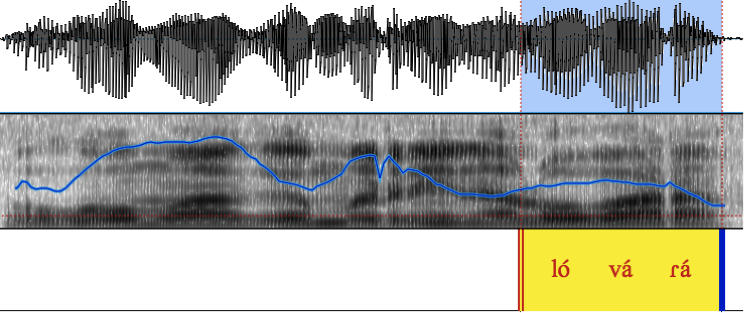
\includegraphics[width=\linewidth]{figures/fig-ch4-1.png}
  \caption{\textit{ogómá gɜmə́rniniə lóvárá} ‘the thief is acting like a guinea fowl.’}
  \label{fig:4-1}
\end{figure}

Words with sequences of LL are pronounced with downdrift, where there is a gradual lowering of f0 across the word, but no sharp fall.

\begin{figure}
  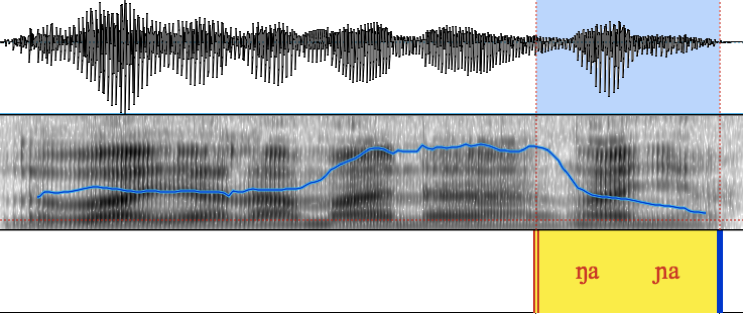
\includegraphics[width=\linewidth]{figures/fig-ch4-2.png}
  \caption{\textit{ləvaja lamáná ŋaɲa} ‘the poor people are cooking grass’}
  \label{fig:4-2}
\end{figure}

Falling tones are also observed with the affixes \textit{-lo} (3pl), \textit{-ja} (inst) and \textit{-u} (loc) which attach at the end of verbs. In general, these affixes cause a H tone to be inserted on the previous syllable if it is otherwise low, as in the following forms:

\ea
\begin{tabular}[t]{ll}
kɜd̪ɜ́t̪ːurt̪iə 	&	‘he’s waiting for it’\\
kɜd̪ɜ́t̪ːurt̪iá\textbf{-lo} 	&	‘he’s waiting for them’\\
katóŋóðeá\textbf{-ja} 	&	‘he’s taking care of it’\\
\end{tabular}
\z

When the previous syllable is a single H tone, however, a falling tone occurs on the suffix:

\ea
\begin{tabular}[t]{lll}
g-a-lat̪-ó 		&	[galat̪ó]	&	‘he molded it’\\
g-a-lat̪-ə́-lo 	&	[galat̪ə́lô]	&	‘he molded them’\\
\end{tabular}
\z

When the verb forms have a sequence of H tones preceding, there is no falling tone, and the suffixes are low-toned. 
\ea
\begin{tabular}[t]{ll}
g-a-lát̪-á 		&	‘he is molding it’ \\
g-a-lát̪-á-lo 	&	‘he is molding them’ \\
t̪úŕt̪-ú			&	‘wait for it!’ \\
t̪úŕt̪-ə́-lo 		&	‘wait for them! \\
\end{tabular}
\z

\section{Tone distribution}
The tone patterns of nouns and verbs are different. Nouns show a range of different high and low lexical sequences. Verb roots do not contrast for lexical tone. Instead, grammatical tone is imposed on verb stems. We will leave discussion of verb tone for the verb section X when aspect, mood and deixis are outlined. 

In the noun system, the main restriction on tone distribution is that two high tones separated by a low cannot occur within a single root (including noun class markers). Exceptions to this are reduplications, such as \textit{ləɲáləɲá} ‘sandstone’. Adjacent sequences of H tone are possible, and the restriction can therefore be analyzed as one single autosegmental H tone per word, assuming that tone sequences consist of a single H tone that is spread to other vowels. The tone patterns observed are as follows.

\ea
\begin{tabular}[t]{llll}
LL	&	&	HH \\\hline
nala	&	'grinding stones'	&	ðáɾá	&	'rope'\\
ləmbi	&	'loincloth'			&	léɲá	&	'egg, penis'\\
oða		&	'deer sp.'			&	ɜ́dí		&	'skin'\\
abəl	&	'bird sp. that hangs upside down'	&	ðə́wáð	&	'buffalo'\\
&\\
LH	&	&	HL\\\hline
ləbú	&	‘well’	&	óna		&	‘small basket’\\
ŋusí	&	‘chick’	&	ðóla		&	‘rat’\\
ɜðú		&	‘breast’&	lóloŋ	&	‘string’\\
ɲogə́l	&	‘eagles’&	élːe	&	‘feather’\\
\end{tabular}
\z

The HL pattern is not as common as the others, and it is often associated with an initial heavy syllable. The LH pattern is also commonly found when the final syllable is heavy. However, as can be seen by the examples, this is a tendency rather than a requirement.

Three syllable words have all possible combinations of L and H except for the unattested HLH. Those of the form HLL, HHL and LHL are less common than the others. This suggests a tendency to favor high tone spreading to the end of the word (Jenks \& Rose 2011). 

\ea
\begin{supertabular}[t]{lllp{3.5cm}}
LLL	&	&	HHH\\\hline
ðəvəra	&	‘line’	&	ðə́bʷáðá	&	'incense-producing tree’\\
ebamba	&	'drum’	&	ɜ́mə́ðíə	&	'celebration'\\
laməɾeð	&	‘non-poisonous snake sp.' &	lə́ŋɡə́ŋé	&	‘bell’\\
&\\
LHH	&	&	LLH\\\hline
ðəbéɾá	&	‘cotton’	&	ðəbəgí	&‘animal trap weighted with a large flat stone’\\
ɜðúní	&	‘hearthstone, oven’	&	ɜgəðiə́	&	'mill floor'\\
lambálá	&hut, shelter	&	ləbopwá	&	‘mushroom’\\
&\\
HLL	&	&	LHL\\
ðɜ́ŋguri	&	‘chameleon’	&	ðəgívi	&	‘bread’\\
ógəŋːa	&	'plant that causes itching'	&	ɜt̪úlɜ	&	‘big spear’\\
áveja	&	'spring, rainy season'	&	lat̪óra	&	‘tomato’\\
&\\
HHL	&	&	HLH\\\hline
ðáŋála	&	‘ewe’	&	$\star$ &\\
lə́búŋwɜ	&	‘water pot, bottle’& &\\
\end{supertabular}
\z

As for words longer than three syllables, similar patterns are found, but again, words with a single H anywhere but the final position are rare. 

\ea
\begin{tabular}[t]{lll}
HHHH	&	ŋə́vándə́ŋé	&	‘type of dried fruit’\\
		&	ɜ́rtə́ŋə́tiə	&	‘armpit’\\
LLLL	&	ŋəmɜgəniə	&	‘work, job’\\
		&	ðabəlat̪a	&	‘thatching tool for smoothing’\\
LHHH	&	ləpə́ndóŋwá	&	‘bushbaby’\\
		&	ŋat̪ábə́lá		&	‘small lock’\\
LLHH	&	lamatáɾá	&	‘support pole’\\
		&	ðəgəmə́níə	&	‘sesame granary’\\
LLLH	&	ed̪apəgá		&	‘nail’\\
		&	ebambəɲá	&	‘skull, eggshell’\\
LLHL	&	ŋavəléka	&	‘mule’\\
		&	aləŋgréma	&	‘bed’\\
LHLL	&	ɜlbɜ́mbɜɾiə	&	‘stool’\\
		&	ləŋɡə́lːəme	&	‘pen, crab’\\
LHHL	&	aɾʧə́ŋála		&	‘broken piece of gourd’\\
		&	aʧóŋgwáɾa	&	‘black bird of prey’\\
HHLL	&	lə́fːə́ɾəŋeə	&	‘bird sp’\\
\end{tabular}
\z

\section{Tone spreading}
There are four tonal spreading rules in Moro, two in the nominal system and two associated with verbs.

In the nominal system, a H tone spreading rule is observed with the instrumental/comitative suffix \textit{-Ca}. The C indicates that the consonant agrees in noun class (Jenks \& Rose 2011). The tone of the suffix matches that of the final syllable of the noun. This can be analyzed as tone spreading from the noun stem to the suffix. 

\begin{table}
\caption{Instrumental –Ca}
	\begin{tabular}[t]{llllll}
		Final H & & &  Final L\\\hline
LH-H	&	ɜðú-já	&	‘breast'	&	LL-L		&	eða-ɡa	&	‘meat’\\
HH-H	&	ŋíní-ŋá	&	‘dog’	&	HL-L		&	ðót̪oŋ-ða	&	‘agama lizard’\\
LLH-H	&	ðəŋəlá-ðá	&	‘tongue’	&LLL-L	&	ðamala-ða	&	‘camel’\\
LHH-H	&	ðəbáɾá-ðá	&	‘cotton’		&	HLL-L	&	áveja-ga	&	‘spring’\\
HHH-H	&	ŋə́və́ní-ŋá		&	‘blood’		&	LHL-L	&	padóla-ða	&	‘jute’ \\
	\end{tabular}
  \label{tab:ch4:2}
\end{table}

The locative prefix \textit{é-} (allomorphs: í, ék-, és-, ég-, ík, ís-, íg-) spreads high tone rightwards. There are two possible variants of this rule. Either the high tone may spread once to the following syllable, or it may spread to the end of the noun stem (excluding other suffixes), as shown below. In both cases, if the noun contains a LH sequence, H tone spreading halts one syllable away to avoid placing two H tones adjacent to teach other, ex. \textit{ðəŋəlá  é-ðə́ŋəlá}.

\begin{table}
	\begin{tabular}[t]{llllll}
Noun	&	locative		&	&			Noun		&	locative		&	\\\hline
ðaba	&	é-ðábá		&	cloud	&	ðəŋəlá	&	é-ðə́ŋəlá		&	tongue\\
ðamala	&	é-ðámálá	&	camel	&	ogovélá	&	ék-ógovél	&	monkey\\
ŋíní 	&	í-ŋíní		&	dog		&	ðót̪oŋ 	&	é-ðót̪oŋ		&	agama lizard\\
ŋə́və́ní	&	í-ŋə́və́n		&	blood	&	áveja	&	ék-áveja		&	spring\\
ŋə́ðə́máná	&	é-ŋə́ðə́mán		&	beans	&	ðáŋála	&	é-ðáŋála	&	sheep\\
etám	&	ég-ətám		&	neck		&	eváɾt̪ə́ŋé	&	ék-əváɾt̪ə́ŋ	&	type of tree\\
ðəbáɾá	&	é-ðəbáɾá	&	cotton	&	ləŋɡɜ́lːəme	&	é-ləŋɡɜ́lːəme	&	pen\\
padóla	&	é-padóla	&	jute		&	aʧóŋgʷára	&	ég-aʧóŋgʷár	&	‘bird of prey’\\
	\end{tabular}
	\caption{Locative é-}
	\label{tab:ch4:3}
\end{table}

The addition of this prefix can condition loss of the final vowel. See details of this prefix in section X.

In the verbs, there are two patterns of H tone spreading. One involves H tone on the stem in proximal imperfective and dependent clause verb forms. The second involves H tone spread from a final perfective vowel to a following object. 

If a verb root is of the shape CVC, H tone appears on the root in the proximal imperfective and in dependent clause forms. This H tone is spread or extended one syllable to the right for most verbs. This is typically to the final aspect suffix, \textit{-a} or \textit{-eə} (or vowel harmony variants [ɜ], [iə]). 

\ea
\begin{tabular}[t]{llll}
H-H pattern		&				&	H-L pattern		&	\\
g-ɜ-sɜ́ð-ɜ́		&	‘defecate’	&	g-a-tóð-a		&	‘move’\\
g-a-wáð-á		&	‘poke’		&	g-a-váð-a 		&	‘shave’\\
g-a-nát̪-á		&	‘taste’		&	g-a-sát̪-a		&	‘chew’\\
g-a-bwáɲ-á		&	‘like, wantʼ	&	g-a-nwán-a		&	‘watch’\\
\end{tabular}
\z

However, if the passive, anti-passive or benefactive applicative suffix appears before the final aspect suffix, it will host the H tone. This is the case with both kinds of short verbs:

\ea
\begin{tabular}[t]{llll}
	&	Imperfective	&	Imperfective passive &	\\
H-H &	g-a-bwáɲ-á		&	g-ɜ-bwɜ́ɲ-ə́n-iə		&	‘like, want’\\
	&	g-a-wáð-á	&	g-ɜ-wɜ́ð-ə́n-iə		&	‘poke’\\
H-L	&	g-a-váð-a	&	g-ɜ-vɜ́ð-ə́n-iə		&	‘shave’\\
	&	g-a-tóð-a	&	g-ɜ-túð-ə́n-iə	&	‘move’\\
\end{tabular}
\z

If a perfective verb is followed by an object beginning with a low tone, H tone spreads from the perfective to the following object, as in (19)c,d:

\ea
\begin{xlist}
	\ex \gll l-a-mámː-atʃəð-a ŋavəɾa\\
			\textsc{sm}.\textsc{cl}l-\textsc{rtc}-\textsc{iter}-take-\textsc{recip}-\textsc{impv} \textsc{cl}ŋ.stick\\
			\trans	‘they are taking sticks from each other’
	\ex \gll l-a-pə́g-á 	lugi 	loaɲa\\
			\textsc{sm}.\textsc{cl}l-\textsc{rtc}-uproot-\textsc{impv} \textsc{cl}l.tree	\textsc{cl}l.many\\
			\trans	‘they are uprooting a lot of trees’
	\ex \gll	l-a-mː-atʃəð-ó 				ŋávəɾa\\
			\textsc{sm}.\textsc{cl}l-\textsc{rtc}-take-\textsc{recip}-\textsc{pfv}		\textsc{cl}ŋ.stick\\
			\trans	‘they took sticks from each other’
	\ex \gll l-a-pəg-ó 	lúgi 	loaɲa\\
			\textsc{sm}.\textsc{cl}l-\textsc{rtc}-uproot-\textsc{pfv}	\textsc{cl}l.tree	\textsc{cl}l.many\\
			\trans	‘they uprooted a lot of trees’
\end{xlist}
\z

Other verb forms that have already undergone H tone spreading within the verb stem, such as the imperfective, do not condition this cross-word spreading (19)b.

As all these examples involve restrictions on H tone or H tone spreading, and contour tones do not appear phonologically, Jenks \& Rose (2011) analyze Moro as a H/0 tone system where low tone is not specified with an autosegmental tone. In all cases of high tone spreading, it is in the progressive or rightward direction. There are no observed cases in the language of high tone spreading leftwards. 

\section{Downstep}
Downstep, or the lowering of a H tone adjacent to another H tone, is observed at some word and stem boundaries in Moro. H tones do not generally delete, but they can lower.

The perfective high tone spreading rule discussed in section 4.4 does not apply if the following noun begins with a high tone. In this case, downstep occurs on the object.

\ea
\begin{xlist}
	\ex
	\gll	l-a-pəg-ó 	$^{\downarrow}$nə́deə́	 noaɲa\\
		\textsc{sm}.\textsc{cl}l-\textsc{rtc}-uproot -\textsc{pfv}	\textsc{cl}n.doleib palm 	\textsc{cl}n.many\\
	\trans ‘they uprooted a lot of doleib palm trees’
	\ex
	\gll	ŋerá	ŋalagó 		$^{\downarrow}$ŋwóréðá\\		
		\textsc{cl}ŋ.girl	\textsc{sm}.\textsc{cl}ŋ-\textsc{rtc}-plant-\textsc{pfv}	\textsc{cl}ŋ.sesame seed\\	
	\trans ‘the girl planted sesame seeds’
\end{xlist}
\z

This can be seen in the following sentence in which the HHH object \textit{ŋwóɾéðá} shows a drop of the H tones to a mid f0 range following the final H of the verb, but not as low as the low tones of the verb \textit{ŋalagó} preceding it. The final syllable of the sentence shows a falling tone as discussed above.

\begin{figure}
  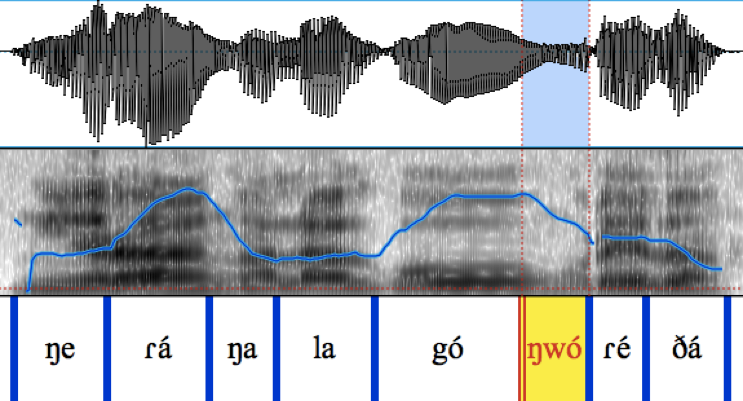
\includegraphics[width=\linewidth]{figures/fig-ch4-3.png}
  \caption{\textit{ŋerá ŋalagó ŋwóréðá} ‘the girl planted sesame seeds’}
  \label{fig:4-3}
\end{figure}

The other environments for downstep occur within the verb stem. 

\section{Tone stability}
Moro shows tonal stability. If a vowel bearing a single H tone is deleted, the H tone appears on a neighboring vowel or sonorant, a phenomenon referred to as tonal stability Tonal stability occurs when vowels are juxtaposed across morphemes or word-boundaries, and the first vowel deletes. Compare the forms in (a) and (b). In the latter, the subject relative clause marker \textit{é-} is deleted due to the following vowel-initial root, but its high tone appears on the [o] of the root. In (d), the object marker \textit{ɲé-} loses its vowel, and the high tone is recuperated on the preceding vowel rather than the following, a pattern which appears to be unique to high-toned object markers. 

\ea
\begin{tabular}[t]{lll}
g-a-ogət̪-ó	&	[kogət̪ó]	&	‘s/he jumped’\\
g-é-ogət̪-ó	&	[kógət̪ó]	&	‘…. who (sg.) jumped’\\
g-ɜ-ɜwut̪-ɜ	&	[kɜwút̪ɜ]	&	‘he is about to drop something’\\
g-ɜ-ɲé-ɜwut̪-ɜ&	[kɜ́ɲɜwut̪ɜ]	&	‘he is about to drop me’\\
\end{tabular}
\z

In each case, however, the high tone appears on another host.

In running speech, the same effect is observed across word boundaries:

\ea	lapəgúgi\\
	\gll l-a-pəg-ó ugi 	 \\
	\textsc{sm.cll}-\textsc{rtc}-uproot-\textsc{pfv}	 clg.tree	 \\
	\trans ‘they are uprooting tree’
\z

\section{Intonation}
Intonation interacts with the lexical tone of the utterance, but in a circumscribed manner. In general, the lexical tones are maintained and the entire pitch is raised, except in the utterance-final position. 

Declarative utterances and yes/no questions (those to which the response is yes or no) are distinguished by i) a question particle and ii) overall pitch raising. Yes/no questions are often marked with an \textit{-a}, which attaches to the final word in the question. However, the particle is optional, and is not obviously present on words than end in [a]. The two types of utterances are otherwise distinguished by pitch. Yes/no questions show raised pitch throughout the utterance, falling during the final word. Speakers differ in whether the final fall in pitch occurs over the whole final word or is confined to the final syllable. 

Consider the following two utterances and the pitch tracks associated with them. The higher (black) pitch track is a yes/no question, and the lower (red) pitch track is the declarative utterance. The two utterances are identical in terms of segments and lexical tones, but differ in overall pitch. The question has much higher overall pitch than the declarative, although both fall in utterance final position. This shows that questions do not show final raising. The tone peak represents both H tones on \textit{máná}

\begin{figure}
  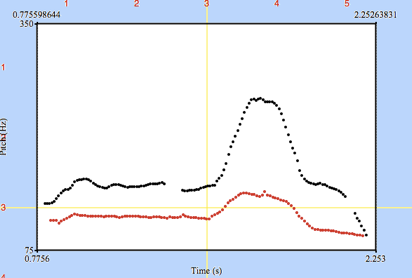
\includegraphics[width=\linewidth]{figures/fig-ch4-4.png}
%   \caption{\gll ləvaja     l-a-mán-á                       ŋaɲa\\
% \textsc{cl}l.poor \textsc{sm.cll}-\textsc{rtc}-cook-\textsc{impv} \textsc{cl}ŋ.grass\\
% \trans Black = question, Red = declarative}
\caption{}
  \label{fig:4-4}
\end{figure}

This example is similar, but each word has H tones, and each of the H tone peaks are higher in the question version of the utterance.

\begin{figure}
  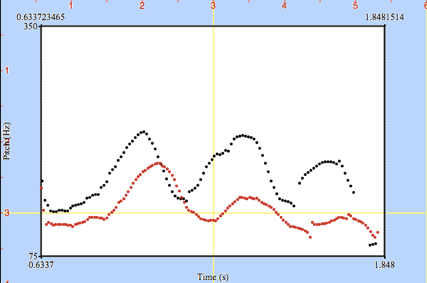
\includegraphics[width=\linewidth]{figures/fig-ch4-5.png}
%   \caption{\gll ŋəməná ŋamə́nwá ŋgárá\\
% \textsc{cl}ŋ.baby goat \textsc{sm}.\textsc{cl}ŋ-\textsc{rtc}-lick-\textsc{impv} \textsc{cl}ŋ.salt\\ \trans }
\caption{}
  \label{fig:4-5}
\end{figure}

% TODO Question MORE NEEDED ON INTONATION
\chapter{Phonological Processes}

In this chapter, we describe the segmental processes in Moro, those that affect vowels, consonants or the interaction between them. 

\section{Consonant-vowel interaction}

\subsection{Palatalization}
Palatalization describes the process whereby consonants are articulated with a palatal off glide [j] (ex. k\super{j}), or shift their articulation to the palatal region, often with a change in manner of articulation. 

The vowel /e/ triggers palatalization of a preceding consonant, adding an off-glide. This affects all consonants except /w/ and /j/. This is an automatic process and will not be indicated in further transcriptions.

\ea
\begin{tabular}[t]{lll}
	élːe	&	[éljːe]		&	‘feather’\\
	ámə́géə	&	[ámə́gjéə] 	&	‘scar’\\
	ðegə́mé	&	[ðjegə́mjé] 	&	‘jaw’\\
	ŋelá	&	[ŋjelá]		&	‘oil’\\
\end{tabular}
\z

The dental stops /t̪/ and /d̪/ are palatalized when followed by the causative suffix \textit{-i}, the passive suffix \textit{-ən}, and the benefactive applicative suffix \textit{-ət̪}, as shown in \tabref{tab:ch5:pal}. Verbs which exceptionally do not show palatalization are given in \tabref{tab:ch5:nopal}. All three suffixes also trigger vowel harmony. No other schwas or [i] trigger palatalization in the language, so this is a lexical process. 

\begin{table}
\begin{tabular}[t]{lllll}
\lsptoprule
&	Perfective	&	Causative perf.	&	Passive perf.	&	Applicative perf.\\
\midrule 
‘lick’	&	k-a-təŋat̪-ó	&	k-ɜ-təŋɜʧ-í	&	kɜ-təŋɜʧ-in-ú	&	k-ɜ-təŋɜʤ-it̪-ú\\
‘prep. soil’	&	k-a-rat̪-ó	&	k-ɜ-rɜʧ-í	&	k-ɜ-rɜʧ-in-ú	&	k-ɜ-rɜʤ-it̪-ú\\
‘sew’	&	k-a-wat̪-ó	&	k-ɜ-wɜʧ-í	&	k-ɜ-wɜʧ-in-ú	&	k-ɜ-wɜʤ-it̪-ú\\
‘repair’	&	k-a-dogat̪-ó	&	k-ɜ-dugɜʧ-í	&	k-ɜ-dugɜʧ-in-ú	&	k-ɜ-dugɜʤ-it̪-ú\\
‘tend’	&	k-a-rəmwət̪-ó	&	k-ɜ-rəmwəʧ-í	&	k-ɜ-rəmwəʧ-in-ú	&	k-ɜ-rəmwəʤ-it̪-ú\\
‘find’	&	k-a-wːaðat̪-ó	&	k-ɜ-wːɜðɜʧ-í	&	k-ɜ-wːɜðɜʧ-in-ú	&	k-ɜ-wːɜðɜʤ-it̪-ú\\
‘watch’	&	k-a-wəndat̪-ó	&	k-ɜ-wəndɜʧ-í	&	k-ɜ-wəndɜʧ-in-ú	&	k-ɜ-wəndɜʤ-it̪-ú\\
‘jump’	&	k-ogət̪-ó	&	k-ugəʧ-í	&	----		&	k-ugəʤ-it̪-ú\\
‘throw’	&	k-ɜwut̪-ú	&	k-ɜwuʧ-í	&	k-ɜwuʧ-in-ú	&	k-ɜwuʤ-it̪-ú\\
‘enter’	&	k-ənt̪-ú	&	k-ənʧ-í	&	k-ənʧ-in-ú	&	k-ənʤ-it̪-ú\\
‘dance’	&	k-a-ɾət̪-ó	&	k-ɜ-ɾəʧ-í	&	---	&	k-ɜ-ɾəʤ-it̪-ú\\
‘close’	&	k-a-land̪-ó	&	k-ɜ-lɜnʤ-í	&	k-ɜ-lɜnʤ-in-ú	&	k-ɜ-lɜnʤ-it̪-ú\\
‘send’	&	k-a-d̪oat̪-ó	&	k-ɜ-d̪uɜʧ-í	&	k-ɜ-d̪uɜʧ-in-ú	&	k-ɜ-d̪uɜʤ-it̪-ú\\
\lspbottomrule
\end{tabular}
\caption{Palatalization triggered by extension suffixes} \label{tab:ch5:pal}
\end{table}

\begin{table}
\caption{Exceptions with no palatalization}\label{tab:ch5:nopal}
\begin{tabular}[t]{lllll}
\lsptoprule
&	Perfective	&	Causative perf.	&	Passive perf.	&	Applicative perf.\\
\midrule
‘drink’	&	kɜ-t̪-ú	&	kɜ-t̪-í	&	kɜ-t̪-ən-ú	&	kɜ-t̪-ət̪-ú\\
‘cough’	&	kɜ-t̪und̪-ú	&	kɜ-t̪und̪-í	&	-----	&	kɜ-t̪und̪-ət̪-ú\\
‘plant’	&	ka-kad̪-ó	&	kɜ-kɜd̪-í	&	kɜ-kɜd̪-ən-ú	&	kɜ-kɜd̪-ət̪-ú\\
\lspbottomrule
\end{tabular}
\end{table}

If the passive suffix follows the applicative, it can trigger palatalization of the applicative: \textit{k-ɜnd-iʧ-in-ú} ‘it was caught for’.

Other sequences of [t̪] or [d̪] followed by [i] do not show palatalization:

\ea
\begin{tabular}[t]{llll}
	ðɜ́ŕt̪í	&	‘anus’	&	uməɾt̪ín	&	‘co-wife’\\
	it̪əlí	&	‘year’	&	id̪əvíní	&	‘shoe’\\
	kɜt̪iðú	&	‘s/he threaded’
\end{tabular}
\z

The proximal subordinate suffix \textit{–i} (a raised version of /-e/) does not palatalize a preceding dental stop, whether that stop is root-final, or is in the applicative affix (c).

\ea
\begin{tabular}[t]{llll}
&	Perfective	&	Subordinate\\
a.&	k-ənt̪-ú		&	... ɜ́ŋ-ə́nt̪-i		&	‘enter’\\
b.&	k-ɜwut̪-ú	&	... ɜ́ŋ-ɜwút̪-i	&	‘throw’\\
c.&	kɜ-kɜd̪-ət̪-ú	&	... ɜ́ŋə́-kɜ́d̪-ə́t̪-i	&	‘plant for’\\
\end{tabular}
\z

The proximal imperfective diphthong suffix \textit{-iə}, which occurs with roots with high vowels, also does not condition palatalization:

\ea
\begin{tabular}[t]{llll}
a.&		kɜt̪úrt̪iə	&	‘s/he is waiting’\\
b.& 	kɜvɜ́ńt̪iə	&	‘s/he is entering’\\
c.&		kɜɾə́mə́ðit̪iə	&	‘s/he is filling a hole’\\
\end{tabular}
\z

The consecutive imperfective complementizer prefix \textit{t̪-́ } occurs word-initially and is also never palatalized, even when followed by the 1st person subject prefix \textit{i-}:

\ea
\begin{tabular}[t]{llll}
a.&		t̪-í-við-ú	&	‘and I vomited’\\
b.&		t̪-í-t̪und̪-ú	&	‘and I coughed’\\
\end{tabular}
\z

In addition to vowels affecting consonants, palatal consonants can also affect vowels. Before the alveopalatal affricates [tʃ] and [dʒ], /a/ is articulated with a palatal off-glide [j]:

\ea
\begin{tabular}[t]{lll}
labatʃó	&	[labajtʃó]	&	‘they lifted’\\
áʧə́vá(ŋ)	&	[ájʧə́váŋ]	&	‘sorghum porridge, food’\\
gadʒə́vá	&	[kajdʒə́vá]	&	‘s/he doesn’t know’\\
\end{tabular}
\z

\subsection{Rounding}
The short central vowels [ə] and [ɘ] are rounded when followed by a labialized consonant, but not in all cases. Consider the following verb paradigms. The labialization of the final root consonant is suppressed before an \textit{-o} or \textit{-u} suffix, but appears to transfer to the vowel of the root in the imperative (9)a-f. However, if there is no labialized consonant, no rounding occurs (9)g-h.

\ea
\begin{tabular}[t]{lllll}
&	imperfective	&	perfective	&	imperative	&\\
a.	&	g-abə́ɾʷ-a	&	g-abəɾ-ó	&	ábə́ɾ-ó	&	‘fly’\\
b.	&	g-abə́t̪ʷ-a	&	g-abət̪-ó	&	ábot̪-ó	&	‘climb up’\\
c.	&	g-ɜ-bə́gw-ɜ	&	g-ɜ-bəg-ú	&	búg-ú	&	‘hit’\\
d.	&	g-ɜ-də́ɾw-ɜ́	&	g-ɜ-dəɾ-ú	&	dúɾ-ú	&	‘stop, stand’\\
e.	&	g-ɜ-tʃə́ndəŋw-ɜ	&	g-ɜ-tʃəndəŋ-ú	&	tʃə́ndúŋ-ú	&	‘go down’\\
f.	&	g-ɜ-múŕkw-ɜ	&	g-ɜ-murk-ú	&	múrk-ú	&	‘roll, slide’\\
g.	&	g-a-bə́ɾ-á	&	g-a-bə́ɾ-ó	&	bə́ɾ-ó	&	‘touch’\\
h.	&	g-a-tʃə́ð-á	&	g-a-tʃəð-ó	&	tʃə́ð-ó	&	‘chop furniture legs’\\
\end{tabular}
\z
In addition, labialized consonants that appear before [ə] or [ɘ] in the root are realized as [u] in the imperative:

\ea
\begin{tabular}[t]{lllll}
&	imperfective	&	perfective	&	imperative\\
a.	&	g-a-mwə́n-á	&	g-a-mwən-ó	&	mwə́n-ó	&	‘suck, lick’\\
b.	&	g-ɜ-mwə́t̪-ɜ	&	g-ɜ-mwət̪-ú	&	mút̪-ú	&	‘sip’\\
c.	&	g-a-wə́t̪-á	&	g-a-wət̪-ó	&	ót̪ó	&	‘choose’\\
d.	&	g-ɜ-wə́ɾ-ɜ́	&	g-ɜ-wəɾ-ú	&	úɾú	&	‘dig, bury’\\
\end{tabular}
\z

This also accounts for the alternation between [uʤí] ‘man/woman’ (Elyasir’s pronunciation) and [wədʒí] ‘woman’ (Angelo’s pronunciation).

The vowel /ɜ/ is rounded to [ɔ] following and preceding labialized consonants. Phonologically it is transcribed as /wɜ/ (see above), but phonetically, it is pronounced [wɔ]. 

\section{Vowels}
In this section, we outline vowel hiatus resolution and vowel harmony.

\subsection{Vowel hiatus resolution}\label{sec:ch5:hiatus}
When two vowels become adjacent due to morpheme concatenation or across word boundaries, the sequence is repaired by deletion, glide formation, or fusion. Across word boundaries and in the verb/adjective morphology, the first vowel is deleted. In nominal morphology, deletion, glide formation and fusion occurs depending on the nature of the vowels.

\subsubsection{Vowel deletion}
Vowel deletion will be addressed first, beginning with sentences. No matter the quality of the two vowels, the first vowel is always deleted and the second one maintained:
\ea Subject + Verb
\z
\ea Verb + Adverb
\begin{tabular}[t]{lll}
	kadaŋó at̪en	&	[kadaŋát̪en]	&	‘he was quiet’\\
\end{tabular}
\z

\ea Verb + Postposition/particle
\z

\ea Verb + Noun
\begin{tabular}[t]{llll}
a.	&	k-a-wːaðat̪-ó  evəla	&	[kawːaðat̪ évəla]	&	‘he found the wild cat’\\
b.	&	k-a-wːaðat-ó  ugi	&	[kawːaðat̪ úgi]	&	‘he found the tree’\\
c.	&	k-uə́ndit̪-ú evəla	&	[kuə́ndit̪ évəla]	&	‘he listened to the wild cat’\\
d.	&	áŋə́-wːaðat̪-e ugi	&	[áŋə́wːaðat̪ ugi]	&	‘(that) he finds the tree’\\
e.	&	ɜ́ŋə́-wːɜð-i ugi	&	[ɜ́ŋə́wːɜð ugi]	&	‘(that) he makes find the tree’\\
f.	&	ɜ́ŋə́-wːɜð-i ɜt̪úli	&	[ɜ́ŋə́wːɜð ɜt̪úli]	&	‘(that) he makes find the spear’\\
\end{tabular}
\z

Word-internally, the same effect is observed. In examples a-f, the root clause markers \textit{a-/ɜ-}, \textit{é-/í-} delete in favor of the first vowel of the root. In examples g-h, the vowel of the object marker is deleted. 

%\ea
\begin{tabular}[t]{llllll}
a.&	k-a-erl-ó		&	/a-e/&	[e]	&	[kerló]		&	‘he walked’\\
b.&	k-ɜ-ilið-ú		&	/ɜ-i/&	[i]	&	[kiliðú]		&	‘he bought’\\
c.&	k-é-aɾ-ó		&	/é-a/&	[á]	&	[káɾó]		&	‘…who cried’	 \\
d.&	k-é-ogət̪-ó		&	/é-o/&	[ó]	&	[kógət̪ó]	&	‘…who jumped’\\
e.&	k-í-ɜnt̪-ú		&	/í-ɜ/&	[ɜ́]	&	[kɜ́nt̪ú]		&	‘…who entered’\\
f.&	k-í-udən-ú		&	/í-u/&	[ú]	&	[kúdənú]		&	‘…who farted’\\
g.&	k-ɜ-ɲí-ɜwut̪-ú	&	/í-ɜ/&	[ɜ]	&	[kɜ́ɲɜwut̪ú]	&	‘he dropped me’\\
h.&	k-ɜ-ŋɜ́-ilið-ət̪-ú&	/ɜ́-i/&	[i]	&	[kɜ́ŋiliðət̪ú]&	‘he bought for you’\\
\end{tabular}
%\z

\subsubsection{Glide formation}
The locative affix \textit{–ánó} triggers glide formation if the first vowel is peripheral /i e u o/ (15)a-d, but vowel deletion if it is central /ə ɜ a/ (15)e-g.

\ea
\begin{tabular}[t]{llllll}
a.&	ðugi-ánó	&	/i-á /	&	[já]&	[ðugjánó]	&	‘inside the plank’\\
b.&	ome-ánó		&	/i-á / 	&	[já]&	[omjánó]		&	‘inside the fish’\\
c.&	umu-ánó		&	/u-á/	&	[wá]&	[umwánó]		&	‘inside the Arab (derog.)’\\
d.&	ŋombogó-ánó	&	/o-á/	&	[wá]&	[ŋombogwánó]&	‘inside the calf’\\
e.&	utɾə-ánó	&	/ə-á/	&	[á]	&	[utɾánó]	&	‘inside the pig’\\
f.&	ɜwíɾɜ-ánó	&	/ɜ-á/	&	[á]	&	[ɜwíɾánó]	&	‘inside the tree sp.’\\
g.&	aŋorá-ánó	&	/á-á		&	[á]	&	[aŋoránó]	&	‘inside the elephant’\\
\end{tabular}
\z

% TODO Data When this marker appears on the verb in verb + particle combinations the same effects are observed.

\subsubsection{Vowel fusion}
The demonstrative suffix \textit{-íCːi} (C = noun class concord consonant) shows reduction to [ə] with peripheral vowels (16)a-d or vowel fusion with central vowels (16)e-f.

\ea
\begin{tabular}[t]{llllll}
a.&	ðugi-íðːi	&	/i-í/&	[ə́]	&[ðugə́ðːi]	&‘this plank’\\
b.&	ome-íkːi	&	/e-í/&	[ə́]	&[omə́kːi]	&‘this fish’\\
c.&	ɜðu-ísːi	&	/u-í/&	[ə́]	&[ɜðə́sːi]	&	‘this breast’\\
d.&	ŋombogó-íŋːi&	/ó-í/&	[ə́]	&[ŋombogə́ŋːi]&	‘this calf’\\
e.&	ðuwːɜ-íðːi	&	/ɜ-í/&	[ɜ́]	&[ðuwɜ́ðːi]	&‘this smoke’\\
f.&	ðapa-íðːi	&	/a-í/&	[ɜ́]	&[ðapɜ́ðːi]	&‘this friend’\\
\end{tabular}
\z

It is hard to tell which vowel has been deleted since all peripheral vowels may reduce to [ə] (Gibbard et al 2009). When V1 is central, however, vowel fusion appears to take place, producing a central, but raised [ɜ].

\subsection{Vowel reduction}\label{sec:ch5:vreduction}
The high vowels /i u/ centralize and reduce to [ɘ] and the mid vowels /e o/ may reduce to [ə]; they are both transcribed here as [ə]. Vowel reduction is variable, but occurs between consonants. It is often triggered by the addition of affixes, but may also occur across words, particularly in the verb - object configuration.

\ea Between words
\begin{tabular}[t]{ll}
kaɾənó ŋáwá  $\rightarrow$ [kaɾənə́ ŋáwá]	&	‘s/he swallowed water’\\
\end{tabular}
\z

Singular forms that begin with one of the vowels /i e u o/ show reduction to [ə] with the addition of a plural prefix /n-/:

\ea
\begin{tabular}[t]{llll}
&	singular&	plural\\
a.&	ibəgwɜ́	&	n-əbəgwɜ́	&	‘back of knee’\\
b.&	ebamba 	&	n-əbamba		&	‘drum’\\
c.&	uməní 	&	n-əmwəní 	&	‘tree sp.’\\
d.&	otʃːa 	&	n-ətʃːa 	&	‘milk pot’\\
\end{tabular}
\z

Reduction occurs after the progressive prefix \textit{v-} in (19)a, and locative prefix \textit{ék-/ík-} in (19)b,c. The object marker \textit{ɲé} causes reduction of the preceding vowel /ó/ when attached as a suffix in (19)d, but it reduces itself when attached as a prefix in (19)e.

\ea Affixes
\begin{tabular}[t]{lllll}
  	a.& gilíðɜ \~ gɜvə́líðɜ	&	‘s/he is buying’\\
	b.&	iɾə́ŋ 				&	‘name’	&	ík-əɾə́ŋ		&	‘in name’\\
	c.&	ebamba				&	‘drum’	&	ék-ə́bámbá		&	‘in drum’\\
	d.&	lanatʃó-ɲé lavəðá  	&[lanatʃə́ɲé lavəðá]	&	‘s/he gave me a fig’\\
	e.& la-ɲé-natʃa lavəðá	&[laɲə́natʃa lavəðá]	&	‘s/he is about to give me a fig’\\
\end{tabular}
\z

\subsection{Epenthesis}\label{epenthesis}
The vowel [ə] (or [ɘ] under harmony) is inserted to break up consonant sequences, and to aid in the pronunciation of initial geminates. Some verb roots begin with geminate consonants. When they occur in the imperative with no prefixes, [ə] is inserted before obstruent geminates. There are also some nouns that appear to have epenthetic vowels.

\ea
\begin{tabular}[t]{llll}
Verbs	&	&	Nouns\\
ə́sːó	&	‘eat!’	&	ɘ́sːí	&	‘eye’\\
ɘ́pːú	&	‘beat!	&	ə́rːá	&	‘lizard’\\
ɘ́wːí	&	‘boil!’	&	ɘ́sːiə́	&	‘fire’\\
ə́t̪ːú	&	‘drink!’	&	əwːɜgɜ́	&	‘threshing floor’\\
\end{tabular}
\z

The other case of initial [ə] involves consonant sequences with initial liquids: /rl/ /rm/ /ɽt/ /ln/, /lt/, /lt̪/ and /ld̪/. These sometimes alternate with CəC. They may be considered epenthesis or metathesis (switching of ə and the first consonant). 

\ea
\begin{tabular}[t]{lll}
əCC	&	CəC\\
ə́rl-ó	&	g-a-rə́l-á	&	‘bear fruit/have rash, scabs’\\
ə́rlát̪-ó	&	g-a-rə́lát̪-a	&	‘stomp, trample’\\
ərmeə	&				&	‘rib’\\
ə́ɽtú		&				&	‘gazebo, shade structure\\
əlná	&	lənːá		&	‘room’\\
əltú		&				&	‘shelter’\\
ə́ltóléa		&				&	‘cheek, shouting’\\
əltúr		&				&	‘umbilical hernia’\\
ə́ltə́miə́		&				&	‘barren woman’\\
ə́lt̪ə́miə́		&				&	‘termite mound’\\
ə́ld̪ə́máná		&				&	‘bean’\\
\end{tabular}
\z

Epenthesis also occurs between consonant sequences that arise through morpheme concatenation.

% TODO Sharon INSERT EXAMPLES

\subsection{Vowel harmony}\label{section:vharmony}
Thetogovela Moro has a vowel harmony system that is productive, even applying to loanwords. The ‘lower’ set of vowels /e a o/ raise to the higher counterparts /i ɜ u/ respectively. In addition, phonetic evidence suggests that there are two kinds of schwa, a lower /ə/ which patterns with /e a o/, and its alternate, a higher /ɘ/ that groups with /i ɜ u/ according to harmony (see Ritchart \& Rose 2017 for more details).

Unlike other Kordofanian languages, such as Laru (REF) or Acheron (REF), we have not found evidence for  contrastive distinctions within the same height category, such as /e/ and /ɛ/ or /i/ and /ɪ/, contrasts which are assumed to involve the feature Advanced Tongue Root (ATR).

Vowel height can be measured acoustically by using the first formant. A low first formant (F1) corresponds to a higher vowel, whereas a high F1 corresponds to lower vowel. Vowel backness corresponds to the second formant, or F2; low F2 corresponds to a backer vowel. The mean F1 and F2 values of the vowels for for four speakers (three male, one female) are given below. The higher vowels [i] and [u] have a lower F1 (avg. 330-350Hz)  than their lower mid counterparts [e] and [o] and the mid central vowel [ɜ] (avg. 449-455), a difference of about 100 Hz. The vowel [ɜ] has a lower F1 than the low vowel [a] (avg. 643), a difference of about 200 Hz. Finally, the  central vowel [ɘ] has an F1 slightly higher than the high vowels, by about 20Hz, while the F1 of [ə] is slightly higher than the mid vowels, again by about 20Hz. The difference between the two short central vowels is about 100Hz. 

Mean F1 and F2 values of the vowels 
\begin{table}
  \begin{tabular}{lllll}
    \lsptoprule
	Vowel &	Mean F1 &	Standard Deviation	&	Mean F2 &	Standard Deviation	\\
	\midrule
	i	&   330.4	&	38.6		&	2212.8	&	175.3 \\
	e	&	453.9 	&	66.2		&	2076.2	&	  233.1	\\
	u	&	350.0	&	43.1		&	1025.4	&	280.5	\\
	o	&	449.3 	&	61.9		&	990.7	&	213.0	\\
	ɘ	&	372.3	&	54.9		&	1415.4	&	327.6	\\
	ə	&	479.7 	&	68.3		&	1297.7	&	263.2	\\
	ɜ	&	455.7	&	52.5		&	1711.1	&	255.5	\\
	a	&	642.9 	&	87.0		&	1464.5	&	206.1	\\
\lspbottomrule
  \end{tabular}
  \caption{F1 \& F2 of vowels}
  \label{tab:ch2:2}
\end{table}


The figure shows that [i] has a lower F1 (hence is a ‘higher’ vowel) than [e] and the same goes for the comparison between [u] and [o]. In general, back vowels have higher F1 than front vowels. The mid-front-central vowel [ɜ] has lower F1 than the low-central [a]. The vowel [ɘ] is positioned as a high-mid vowel compared to the high and mid front vowels [i e] and high and mid back vowels [u o. The vowel [ə] is a mid-low vowel compared to the mid vowels [e] [o] and [ɘ] and the low vowel [a]. 

\begin{table}
	\begin{tabular}[t]{llllll}
	\lsptoprule 
Vowel	&	Mean F1	&	Standard Deviation	&	Mean F2	&	Standard Deviation\\
i   	&	293.23	&	25.96	&	2263.32	&	125.49\\
u	&	343.13	&	38.45	&	1042.03	&	166.41\\
ɘ	&	365.21	&	49.03	&	1253.44	&	253.10\\
ɜ	&	414.62	&	50.55	&	1737.46	&	171.09\\
\lspbottomrule 
	\end{tabular}
	\caption{Mean F1 of higher vowels}
	\label{tab:ch5:1}
\end{table} 

\begin{table}
	\begin{tabular}[t]{llllll}
	\lsptoprule 
Vowel	&	Mean F1	&	Standard Deviation	&	Mean F2	&	Standard Deviation\\
e	&	379.67 	&	55.58	&	2030.30	&	85.58\\
o	&	426.08 	&	65.16	&	1068.93	&	133.06\\
ə	&	445.77 	&	44.09	&	1154.88	&	179.26\\
a	&	556.87 	&	74.29	&	1477.02	&	127.66\\
\lspbottomrule 
	\end{tabular}
	\caption{Mean F1 of lower vowels}
	\label{tab:ch5:2}
\end{table} 

\begin{figure}
  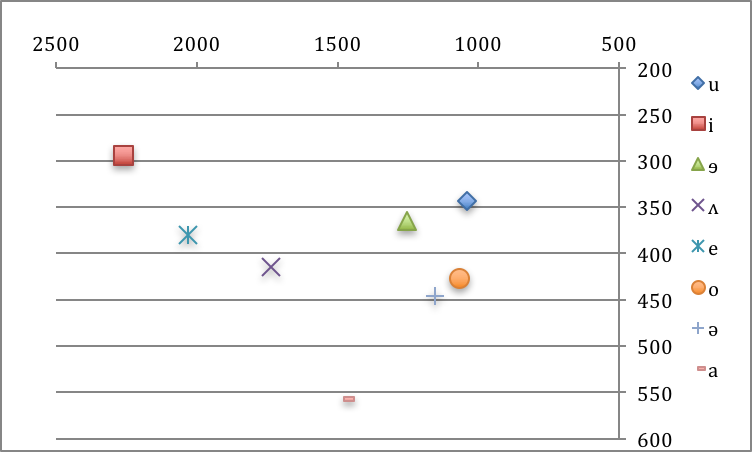
\includegraphics[width=\linewidth]{figures/fig-ch5-1.png}
  \label{fig:5-1}
\end{figure}

The vowel ɜ is acoustically in the mid range, even though it patterns with the higher vowels for the purposes of vowel harmony. Allowing for the fact that back vowels are generally lower than front vowels acoustically, the vowels fit into the basic descriptive categories as follows:

\ea
\begin{tabular}[t]{llll}
&	front	&	central	&	back\\
high	&	i	&	&	u\\
high-mid	&	&	ɘ\\
mid 	&	e	&	ɜ	&	o\\
low-mid	&	&	ə\\
low	&	&	a\\
\end{tabular}
\z

We treat the vowels ə and ɘ as central because they can be subject to some coarticulation. The examples in the above chart were followed by back round vowels, which lowered their F2. 

The vowel harmony system can be understood by examining prefixes and suffixes that alternate depending on harmony. Harmony pervades the nominal and verbal systems. In both, the root controls harmony, but in both systems, there are some suffixes that condition raisin.

\subsubsection{Vowel harmony in noun stems}
Prefixes that attach to nouns harmonize with the vowels of the noun stem. The locative prefix that appears on nouns is a clear example. This prefix may be either [e] or [i] in accordance with the vowels of the noun stem. In these examples, there is a single vowel in the root. If the noun stem contains one of the vowels from the set /e a o ə/, the prefix is [e], whereas if the noun stem contains one the vowels from the set /i ɜ u ɘ/, the prefix is [i]. 

\ea
\begin{tabular}[t]{llllll}
	a.&	é-rló		&	‘in the female goat’		
	&	e.&	í-ltú	&	‘in the shelter’\\
	b.&	é-ðáð		&	‘in the path’		&	f.&	í-ðí	&	‘in the thorn’\\
	c.&	é-ðéj		&	‘in the hand’		&	g.&	í-ɽŕwɜ́	&	‘in the goat manure’\\
	d.&	é-ŋgə́m 		&	‘in the squirrel’	&	h.&	í-ŋgwɘ́ɲ	&	‘in the sign’ \\
\end{tabular}
\z

The locative prefix therefore has two realizations that depend on vowel harmony, and the mid [e] and high [i] can be considered harmonic counterparts. Some examples of longer stems with more vowels are given below (note that the prefix ends in [k] before vowel-initial nouns belong to the g-noun class).

\ea
\begin{tabular}[t]{llllll}
	a.&	é-logopáj		&	‘in the cup’		
	&	e.&	í-ŋwulúð	&	‘in the termites’\\
	b.&	é-ðə́gəmjé		&	‘in the jaw’		&	f.&	ík-id̪ɘvín	&	‘in the shoe’\\
	c.&	é-ŋávəléka		&	‘in the mule’		&	g.&	í-ðɜ́ŋguri	&	‘in the chameleon’\\
	d.&	é-lə́və́ɾá 		&	‘in the stick’	&	h.&	íðɘ́púndrí	&	‘in the wood’ \\
\end{tabular}
\z


All the nouns in the above examples show the same harmonic effect on the prefix. Furthermore, they  are themselves composed of vowels from one of the two harmonic sets. Vowels of the 'lower' set /e a o ə/ cooccur whereas vowels of the 'higher' set /i ɜ u ɘ/ cooccur, and there is little mixing.  

Like the locative prefix, the genitive prefix also harmonizes. This prefix is of the shape Ca- (the C represents noun class agreement) or Cɜ-. The prefix attaches to the possessor, but the consonant agrees with the noun class of the possessed. Whether the possessed has high vowels or not does not affect the pronunciation of the genitive prefix. When the vowels of the possessor are from the lower set (/a e o ə/), the prefix is pronounced with the low vowel [a]:

\ea
\begin{tabular}[t]{lll}
	ajén 	&	ja-ŋálːo	&	‘Ngalo’s mountain’\\
	rápá 	&	ra-ŋálːo	&	‘Ngalo’s friends’\\
	ládéə 	&	la-ŋeɾá		&	‘the girl’s hat’\\
	rápá 	&	ra-ŋeɾá		&	‘the girl’s friends’	\\
	lubə́lbə́líə&	la-ŋeɾá		&	‘the girl’s earlobe’\\
	rɜ́gí 	&	ra-ŋeɾá		&	‘the girl’s wounds’\\
\end{tabular}
\z

When the possessor has a higher vowel, however the genitive prefix is realized with [ɜ]
\ea
\begin{tabular}[t]{lll}
	ajén 	&	jɜ-kúku		&	‘Kuku’s mountain’\\
	rápá 	&	rɜ-kúku		&	‘Kuku’s friends’\\
	ŋádéə 	&	ŋɜ-lɘmːiə	&	‘the boys’ hats’\\
	rápá 	&	rɜ-lɘmːiə	&	‘the boys’ friends’\\
\end{tabular}
\z

There are also some noun class prefixes that harmonize. In general noun class prefixes are consonants, and they are categorized according to the type of consonant. However, Gibbard et al (2009) argue that the j noun class is characterized by vocalic prefixes. The singular has the prefix \textit{a-} and the plural the prefix \textit{e-}, as follows:

\ea
\begin{tabular}[t]{lll}
	singular	&	plural\\
	a-jén 	&	e-jén 	&	‘mountain’\\
	á-ɾómá 	&	é-ɾómá 	&	‘black biting ant’\\
	a-t̪ə́ndŕeá&	e-t̪ə́ndŕeá&	‘cloven hoof’\\
	a-bəl	&	e-bəl	&	‘type of bird that hangs upside down’\\
\end{tabular}
\z

If the root has high vowels, the prefixes are \textit{ɜ-} and \textit{i-} respectively:	

\ea
\begin{tabular}[t]{lll}
	singular	&	plural\\
	ɜ-bulúkriə 	&	i-bulúkriə 	&	‘dove’\\
	ɜ-t̪úmí 		&	i-t̪úmí 		&	‘onion’\\
	ɜ-mwəɾíní	&	i-mwəɾíní	&	‘red-necked cobra’\\
	ɜ-ðú		&	i-ðú			&	‘breast’\\
\end{tabular}
\z

Harmony does not affect most nominal suffixes. The instrumental or comitative suffix \textit{–Ca} agrees for noun class with the noun to which it attaches and has the same tone as the final syllable of the noun stem. However, it does not undergo vowel harmony. This is in clear contrast with the genitive \textit{Ca-} prefix, which takes the same segmental shape.

\ea
\begin{tabular}[t]{lll}
	nəbamba-na	&	‘with the drums’	ɜt̪úlɜ-ja	&	‘with the big spear’\\
	áróm-já		&	‘with the anthill’	lɜmí-lá	&	‘with the beard’\\
	emərt̪á-gá	&	‘with the horse’	ŋusí-ŋá		&	‘with the chick’\\
\end{tabular}
\z

The demonstrative suffix is \textit{–íCːi}. It also agrees in noun class with the noun to which it attaches. The initial vowel of the suffix fuses with the final vowel of the noun stem. However, it does not trigger vowel harmony. 

\ea
\begin{tabular}[t]{llll}
ðamala	&	‘camel’		&	ðamalɜ́ðːi	&	‘this camel’\\
lókógóŋ	&	‘scorpion’	&	lókógóŋə́lːi	&	‘this scorpion’\\
ðɘrliə́	&	‘root’		&	ðɘrliə́ðːi	&	‘this root’\\
lútí	&	‘owl’		&	lútílːi		&	‘this owl’	[lútɘ́lːi]\\
\end{tabular}
\z

The same goes for the other demonstrative suffixes, the distal \textit{íCːɜtíCːɜ} and the proximal to hearer \textit{íCːɜj}. 

Possessive pronoun suffixes indicate the person of the possessor. They also agree for noun class, but do not participate in harmony, either as triggers or as targets. Consider the following paradigms:

\ea
\begin{tabular}[t]{ll}
	1\textsc{sg}		&	lókógóŋ-ílːəŋələŋ \\
	1\textsc{dual}	&	lókógóŋ-ílːɜlə́ŋə́li  \\
	2\textsc{sg}		&	lókógóŋ-ílːolːe \\
	3\textsc{sg}		&	lókógóŋ-ílːoŋəloŋ\\
	1\textsc{pl.exc}.&	lókógóŋ-ílːaɲlaɲ  \\
	1\textsc{pl.inc}.&	lókógóŋ-ílːəndr̩ĺi \\ 
	2\textsc{pl}		&	lókógóŋ-ílːalː̩́e \\
	3\textsc{pl}		&	lókógóŋ-ílːenlen\\
\end{tabular}
\z

The possessive suffixes are complex, composed of two components: \textit{íCː}, which may be the demonstrative suffix, and a pronominal-type suffix, which itself is often reduplicated and contains one or two consonants showing noun class agreement. Vowel harmony operates within the second component, so that all the vowels are low or high, but there is no harmony between the \textit{íCː} portion and the second component.

There is one group of suffixes that does participate in harmony, both as triggers and as targets: the inalienable possessives. Inalienable possessives are affixes that indicate inherent possession. In Moro, they attach to kinship terms; these kinship words always appear with a suffix. 

The first four nouns (a-d) all have low vowels, and the suffixes also contain low vowels. There is no vowel harmony observed in the forms in (e-f), even though the noun roots contain high vowels. This is like the behavior observed with other suffixes. However, in (g-h), vowel harmony applies to the \textit{first} vowel of the suffix. The main distinction appears to be the size of the noun stem, which is monosyllabic in (g-h), compared with bisyllabic in (e-f). Harmony in inalienable possession operates rightward, or in the progressive direction, within a two syllable window. 

\ea
\begin{tabular}[t]{lllll}
&	1\textsc{ex}	&	2	&	3\\
a.	&	et̪-áɲ	&	et̪-aló	&	et̪-én	&	‘father’\\
b.	&	was-áɲ	&	was-aló	&	was-én	&	‘wife’\\
c.	&	eváŋg-áɲ	&	eváŋg-áló	&	eváŋg-én	&	‘husband’\\
d.	&	or-áɲ	&	or-aló	&	or-én	&	‘sibling/cousin’\\
e.	&	iðjəŋɡ-áɲ	&	iðjəŋɡ-aló	&	iðjəŋɡ-én	&	‘offspring(sg.)’\\
f.	&	údʌ̪́r-áɲ	&	údʌ̪́r-aló	&	údʌ̪́r-én	&	‘uncle/aunt’\\
g.	&	un-ɜ́ɲ	&	un-ɜló	&	un-ín	&	‘parent-in-law’\\
h.	&	ib-ɜ́ɲ	&	ib-ɜló	&	ib-ín	&	‘sibling-in-law’\\
\end{tabular}
\z

The 1dual inclusive and 1plural inclusive forms are indicated by suffixes with high vowels, which trigger harmony on the root in the regressive direction, observable on the forms in a-d, which contain underlying low vowels.

\ea
\begin{tabular}[t]{llll}
&	1\textsc{dual inc}.	&	1\textsc{pl incl}.\\
a.	&	it̪-ɜlə́ŋ	&	it̪-ɜlə́ŋ-ə́ńdr  	&	‘father’\\
b.	&	wɜs-ɜlə́ŋ	&	wɜs-ɜlə́ŋ-ə́ńdr  	&	‘wife’\\
c.	&	ivɜ́ŋg-ɜlə́ŋ	&	ivɜ́ŋg-ɜlə́ŋ-ə́ńdr  	&	‘husband’\\
d.	&	ur-ɜlə́ŋ	&	ur-ɜlə́ŋ-ə́ńdr  	&	‘sibling/cousin’\\
e.	&	iðjəŋɡ-ɜlə́ŋ	&	iðjəŋɡ-ɜlə́ŋ-ə́ńdr  	&	‘offspring(sg.)’\\
f.	&	údʌ̪́r-ɜlə́ŋ	&	údʌ̪́r-ɜlə́ŋ-ə́ńdr  	&	‘uncle/aunt’\\
g.	&	un-ɜlə́ŋ	&	un-ɜlə́ŋ-ə́ńdr  	&	‘parent-in-law’\\
h.	&	ib-ɜlə́ŋ	&	ib-ɜlə́ŋ-ə́ńdr  	&	‘sibling-in-law’\\
\end{tabular}
\z

The regressive harmony pattern is not restricted in terms of how many vowels it can affect, as seen in (c). Vowel harmony in inalienable possessives is therefore distinct from how harmony operates in other nominal forms. First, it can apply to suffixes, albeit in a restrictive manner, and second, it can be triggered by suffixes and affect roots. The vowel harmony system is therefore not just root-controlled, but exhibits a pattern known as ‘dominant-recessive’, in which one particular harmonic value is dominant. In this case, it is the harmonic value of the high vowels, and this justifies the term ‘raising’ in characterizing the harmony system. 

The domain of vowel harmony in the noun is as follows. Prefixes and inalienable possessive suffixes participate in harmony, but other suffixes do not. 

\ea \textsc{[loc-gen-nc.root-inal.poss]-poss-dem-inst}
\z


\subsubsection{Vowel harmony in verb stems}
Both prefixes and suffixes alternate in harmony according to the harmonic quality of the vowel of the verb root. The following verb forms contain roots with one vowel as well as three affixes: the 1sg subject marker/é-/, the root clause marking prefix /a-/ and the perfective suffix /-ó/.  Roots with the vowel /a e o ə/ co-occur with prefixes and suffixes with these same vowels. However, if the root has a high vowel /ɜ i u ɘ/, then the prefixes and suffixes are raised to their higher counterparts. This type of system can be termed root-controlled. We will justify the form of the underlying vowels and the use of the term ‘raising’ to characterize the harmony when we present suffixes that trigger raising of root vowels. 

\ea
\begin{tabular}[t]{llllll}
&	lower vowels	&		&	& higher vowels.\\
a.&	é-g-a-vað-ó		&	‘I shaved’	&	d.	&	í-g-ɜ-vɜg-ú	&	‘I miscarried’\\
b.&	é-g-a-veð-ó		&	‘I knocked’	&	e.	&	í-g-ɜ-kið-ú	&	‘I opened’\\
c.&	é-g-a-toð-ó		&	‘I woke up’	&	f.	&	í-g-ɜ-t̪urt̪-ú&	‘I waited for’\\
b.&	é-g-a-bəɾ-ó 	&	‘I touched’	&	e.	&	í-g-ɜ-dɘɾ-ú &	‘I stood, covered’\\
\end{tabular}
\z

As with the nouns, all prefixes participate in vowel harmony. These include all subject markers, clause markers, object prefixes, and the durative/iterative reduplicative prefix. The forms below illustrate the subject markers and the root clause marker \textit{a-}, which alternates with \textit{ɜ:}

\ea \textsc{sm.cl}g-\textsc{rtc} -root-\textsc{pfv}\\
\begin{tabular}[t]{lll}
&	‘woke up’	&	‘waited for’\\
1\textsc{sg}	&	é-g-a-toð-ó	&	í-g-ɜ-t̪urt̪-ú\\
2\textsc{sg}	&	á-g-a-toð-ó	&	ɜ́-g-ɜ-t̪urt̪-ú\\
3\textsc{sg}	&	g-a-toð-ó	&	g-ɜ-t̪urt̪-ú\\
1\textsc{du}	&	álə́-g-a-toð-ó	&	ɜ́lə́-g-ɜ-t̪urt̪-ú\\
1\textsc{plexc}	&	ɲá-g-a-toð-ó	&	ɲɜ́-g-ɜ-t̪urt̪-ú\\
1\textsc{plinc}	&	álə́-g-a-toð-ó-r	&	ɜ́lə́-g-ɜ-t̪urt̪-ú-r\\
2\textsc{pl}	&	ɲá-g-a-toð-ó	&	ɲɜ́-g-ɜ-t̪urt̪-ú\\
3\textsc{pl}	&	l-a-toð-ó	&	l-ɜ-t̪urt̪-ú\\
\end{tabular}
\z

More complex forms with object prefixes and the durative/iterative prefix are given below. These verb forms would occur in subject wh-questions of the form ‘who is poking X?’. The clause marker is /é-/, followed by the object prefix, the durative/iterative prefix \textit{CaC-}. All the prefixes harmonize. 

\ea \textsc{\textsc{sm.cl}g-dpc1-om-iter-root-impv}\\
\begin{tabular}[t]{lll}
&	‘.. is poking X’	&	‘..is waiting for X’\\
1\textsc{sg}	&	g-é-ɲə́-ðað-ðəw-a	&	g-í-ɲɘ́-d̪ɜt̪-t̪urt̪-iə\\
2\textsc{sg}	&	g-é-ŋɜ́-ðað-ðəw-a	&	g-í-ŋɜ́-d̪ɜt̪-t̪urt̪-iə\\
3\textsc{sg}	&	g-é-ŋó-ðað-ðəwa	&	g-í-ŋú-d̪ɜt̪-t̪urt̪-iə\\
1\textsc{du}	&	g-é-ndə́-ðað-ðəwa	&	g-í-ndɘ́-d̪ɜt̪-t̪urt̪-iə\\
1\textsc{plexc}	&	g-é-ɲə́-ðað-ðəwa-landa	&	g-í-ŋɘ́-d̪ɜt̪-t̪urt̪-iá-landa\\
1\textsc{plinc}	&	g-é-ndə́-ðað-ðəwa-r	&	g-í-ndɘ́-d̪ɜt̪-t̪urt̪-iə-r\\
2\textsc{pl}	&	g-é-ndə́-ðað-ðəwa	&	g-í-ndɘ́-d̪ɜt̪-t̪urt̪-iə\\
3\textsc{pl}	&	g-é-ðáð-ðəwa-lo	&	g-í-d̪ɜ́t̪-t̪urt̪-iá-lo\\
\end{tabular}
\z

Not all suffixes harmonize. The aspect-mood-deixis suffixes are a single vowel, either /e/, /a/, and /o/, which harmonize to /i/, /ɜ/ or /iə/, and /u/ respectively. 
% TODO ADD FORMS

The ‘extension’ suffixes include a series of suffixes that alter the valence of the verb. They include the following:

\ea
\begin{tabular}[t]{ll}
Antipassive/distributive		&	-əð\\
Locative applicative		&	-at̪\\
Benefactive applicative		&	-ɘt̪\\
Passive 					&	-ɘn\\
Causative					&	-i\\
\end{tabular}
\z

The antipassive is \textit{-əð} and the locative/malfactive applicative is \textit{-at̪}. Both can undergo harmony, although with the former it is difficult to detect due to the short central vowel.

\ea Anti-passive -əð
\begin{xlist}
	\ex \gll é-g-a-mː-əð-ó	\\
		1\textsc{sg}-\textsc{cl}g-\textsc{rtc}-take-\textsc{ap}-\textsc{pfv}  \\			
	\trans ‘I got married’ (= ‘I took someone’) 
	\ex \gll g-a-ðə́w-ə́ð-eə 		\\
		\textsc{sm.cl}g-\textsc{rtc}-poke-\textsc{ap}-\textsc{ipfv}  	\\
	\trans ‘s/he gives injections’ (= s/he pokes distributively)
	\ex \gll g-ɜ-ðúg-ɘ́ð-iə	\\
		\textsc{sm.cl}g-\textsc{rtc}-nurse-\textsc{ap}-\textsc{ipfv}  \\
	\trans ‘she is breastfeeding kids’
\end{xlist}
\z

\ea Locative/malfactive applicative \textit{-at}
\begin{xlist}
	\ex \gll é-g-a-mː-at̪-ó 	ŋeɾá 	ád̪ámá 	\\
		1\textsc{sgsm-cl}g-\textsc{rtc}-take-\textsc{loc.appl}-\textsc{pfv}	\textsc{cl}ŋ.girl	\textsc{cl}g.book  \\
	 \trans ‘I took the book from the girl’
	\ex \gll é-g-ab-at̪-ó 	ád̪ámá 	é-lná \\
		1\textsc{sgsm-cl}g-carry-\textsc{loc.appl}-\textsc{pfv}	\textsc{cl}g.book  	\textsc{loc-cl}l.room\\
	\trans ‘I carried the book into the room’
\end{xlist}
\z
% TODO NEED LOC with vowel raising

The other extension suffixes have high vowels and trigger harmony. Their effect on harmony can be seen in the following examples. The root \textit{kad̪} is raised to \textit{kɜd̪} by the extension suffixes, as well as all the prefixes preceding the root. The following aspect-mood-deixis suffix is also raised, as seen in (c) and (d). 

\ea
\begin{xlist}
\ex \gll	é-g-a-kad̪-ó\\  			
 	1\textsc{sg-cl}g-\textsc{rtc}-plant-\textsc{pfv}\\  			
 	\trans ‘I planted’ 					

\ex \gll 	í-g-ɜ-kɜd̪-í\\
	1\textsc{sg-cl}-\textsc{rtc}-plant-\textsc{caus}.\textsc{pfv}\\
	\trans ‘I made s.o. plant’

\ex \gll	í-g-ɜ-kɜd̪-ɘt̪-ú \\ 				
 	1\textsc{sg-cl}-\textsc{rtc}-plant-\textsc{appl}-\textsc{pfv} \\
 	\trans ‘I planted for s.o.’ 

\ex \gll 	ŋ-ɜ-kɜd̪-ɘn-ú\\
	\textsc{sm.cl}-\textsc{rtc}-plant-\textsc{pass}-\textsc{pfv}\\
	\trans ‘it (corn) was planted’
\end{xlist}
\z

Vowel harmony extends to the beginning of the word, but is more restricted in the progressive direction, affecting only the aspect-mood-deixis suffix. It fails to extend to object markers (b-c) or the instrumental suffix -ja (c-e)

\ea
\begin{tabular}[t]{llll}
a.&	é-ɡ-a-veð-ə́-ŋá		&	‘I slapped you sg.’	 \\
b.&	í-ɡ-ɜ-buɡ-ə́-ŋá		&	‘I hit you sg.’		 \\
c.&	ɡ-ɜ-dɜɾ-ə́-ló-ja		&	‘s/he covered them with it’\\
d.&	ɡ-ɜ-dɜɾ-ə́-ja			&	‘s/he covered it with it’\\
e.&	ɡ-ɜ-dɜɾ-t̪-ú-ɲə́-ŋó-ja	&	‘s/he covered me with it for him/her’\\
\end{tabular}
\z

The locative suffix \textit{-u}, although high, does not trigger raising, but forms a diphthong with the preceding vowel.

\ea
\begin{tabular}[t]{ll}
ɡ-a-və́dað-á-u	&	‘s/he is sweeping in it’\\
\end{tabular}
\z

The domain of vowel harmony is therefore the entire verb excluding the final suffixes (see Rose 2013, Jenks \& Rose 2015). Triggers are italicized. 

\textsc{[COMP-SM-CLASS-CLAUSE-AMD-OM/PROG-ITER-ROOT-AP-LOC.APPL-CAUS-APPL-PASS-AMD]-PL-OM-INST-LOC}

\subsubsection{Vowel harmony in loanwords}
Many Arabic loanwords have been incorporated into Moro, and they conform to the vowel harmony system, too. There are also some words borrowed from English or neighboring Kordofanian languages. With Arabic nouns, the definite article al can be borrowed along with the noun. If the noun is a member of the j/j class, a is reinterpreted as the noun class marker and alternates with e (or ɜ alternates with i with higher vowels) in the plural, ex. \textit{a-ləŋgréma} < /al-ʕangareːb/ has the plural \textit{e-ləŋgréma} and \textit{ɜ-t̪úmí} ‘onion’ < \textit{atːuum} ‘garlic’ has the plural \textit{i-t̪úmí} ‘onions’. If the Arabic word contains mismatched low and high vowels such as \textit{i} and \textit{a}, it is generally the penultimate vowel or the long vowel that determines the harmony pattern. A good comparison is the word for ‘book’, where /aa/ determines the harmony, and that for ‘church’, where the long /ii/ determines the harmony, and raises other vowels:

\ea
\begin{tabular}[t]{llll}
ád̪ámá		&	‘book’	< al kitaab	&	ɜlkɜnísɜ&	‘church’  < al kaniisa	\\
aləŋgréma	&	‘bed’			&	ɜlbɜ́lɜd̪iə	&	‘country’\\
alfásəl		&	‘room’ 			&	ɜlbúní		&	‘coffee’\\
alfəɾáɾa	&	‘small hatchet’	&	ɜt̪úmí		&	‘onion’\\
almoʧána	&	‘tobacco pipe’\\
bantalón	&	‘trousers’\\
&	\\
Exceptions\\
tʃiwáfa		&	‘guava\\
burtugáná	&	‘orange’\\
\end{tabular}
\z

\section{Consonants}
\subsection{Devoicing}
Sonorants and /ð/ are the only consonants routinely found word-finally. /ð/ is devoiced in this position:
\ea
\begin{tabular}[t]{ll}
	laməɾeθ	&	‘non-poisonous snake sp.’\\
	eɾéθ	&	‘piece of clothing’\\
\end{tabular}
\z

There are only a few cases of other obstruents occurring word-finally, due to a word-final vowel that has been deleted. The /g/, but not the /v/ is devoiced:

\ea
\begin{tabular}[t]{ll}
	ekworəv		&	‘even more, additional’\\
	ékomák		&	‘in the snail’	(cf. omágá ‘snail’)\\
\end{tabular}
\z

Geminate obstruents, with the exception of [ðː], are voiceless. If a geminate is formed by juxtaposition of two identical voiced obstruents, devoicing occurs, as in (24)a-d. This happens with the iterative/durative prefix on verbs, which is takes the shape CaC, where the C is a copy of the first consonant of the root. With respect to /v/, the devoicing is optional, but it is obligatory with the stops and affricates:

\ea
\begin{tabular}[t]{llll}
&	3\textsc{pl} imperfective	&	3\textsc{pl} iterative imperfective\\
a.	&	l-a-bə́ɾ-á	&	l-a-báp-pəɾ-a	&	‘touch’\\
b.	&	l-a-də́ŕn-a	&	l-a-dát-tərn-a	&	‘press’\\
c.	&	l-a-ʤóm-á	&	l-a-ʤáʧ-ʧom-a	&	‘move’\\
d.	&	l-a-və́léð-a	&	l-a-váf-fərleð-a	&	‘pull’\\
&&	l-a-váv-vəleð-a\\
e.	&	l-a-ðə́w-á	&	l-a-ðáð-ðəw-a		&	‘poke’\\
\end{tabular}
\z

\subsection{Post-nasal hardening}
The fricative /ð/ is hardened to [d̪] following /n/ or /l/. Distributionally, /ð/ only occurs after rhotics, not after nasals or /l/. Evidence that /ð/ hardens comes from singular and plural nouns. Each singular noun begins with a consonant or a vowel, which is the noun class marker; the plural is marked with a different consonant or vowel. The noun class is determined by this prefix, but also by the concord/agreement markers that appear on the verb or modifying elements. The following pairs show that when the root begins with /ð/, and the prefix is /n/, the /ð/ is realized as [d̪]. Furthermore, the example in c shows that the sequence /l-ð/ can be realized as [nd̪]. This does not always occur, and [ə] may instead intervene to separate the consonants: \textit{ləðwɜ/ŋəðwɜ} ‘trunk of tree sg/pl’

\ea
\begin{tabular}[t]{llllp{4cm}}
&	noun class	&	singular		&	plural	&	gloss\\
a.	&	g/n	&	úðə́pí		&	ńd̪ə́pí	&	‘tree sp. with white flowers (metaphor for grey hair)’\\
b.	&	g/n	&	oða	&	nd̪wa	&	‘deer sp.’\\
c.	&	l/ŋ	&	nd̪əmana	&	ŋəðəmana	&	‘kidney bean’\\
&&	ə́ld̪ə́máná	&	nə́ðə́máná	&	‘bean’\\
\end{tabular}
\z

\subsection{Stop insertion}
The stop [d] is inserted between /n-ɾ/ or /n-r/ sequences. 

\ea
\begin{tabular}[t]{lll}
singular	&	plural\\
úŕðíə	&	ńdŕðíə	&	 ‘gazelle sp.’\\
eɾéθ	&	ndréθ	&	‘clothes’\\
íɾíə	&	ńdríə	&	‘fence, garden’\\
iɾíŋ	&	ndríŋ	&	‘name’\\
\end{tabular}
\z

% TODO What happens when n- attaches to a word beginning with r? n-ɽ?

\subsection{n-l avoidance}
The sequence n-l does not occur in Moro, and when two morphemes come together that juxtapose these two sounds, there are avoidance strategies, where /n/ is unrealized. 

There are several prefixes /n-/ or /nə-/ which fail to appear if the root or stem begins with /l/.
% TODO The noun class prefix /n-/ 

The locative prefix n(ə-) cannot appear before a noun beginning with /l/. For some speakers, there is no prefix and for others, the /n/ assimilates to the following /l/ to form a geminate [lː]. ex. n-ladʒəlea --> lladʒəl 'on the bicycle'. 

\ea
\begin{tabular}[t]{lll}
nə-nəmərt̪á	&	‘on the horse’\\
nə-ðamala	&	‘on the camel’\\
loandra	or lːoandra	&	‘on the stone’	&	*n-loandra\\
\end{tabular}
\z

The complementizer \textit{n(ə́)-} cannot appear on words that begin with /l/. This complementizer optionally appears on subjects and verbs in wh-questions and dependent clauses. In a,b, the \textit{nə́ }can appear, but in c., when the 3\textsc{pl} subject marker is l-initial, it systematically fails to appear. Note that if the plural noun class is changed as in (d), the nə́ appears. 

\ea
\begin{xlist}
	\ex \gll ŋwɜ́ndə́kːi 	nə́-ɡ-ə́-sː-ó	\\
		what.\textsc{cl}g	\textsc{comp}-\textsc{sm.cl}g-\textsc{dpc}2-eat-\textsc{pfv} \\ 
		\trans ‘What did he eat?’
	\ex \gll ŋwɜ́ndə́kːi 	nə́-ɡ-ə́-sː-ó	\\
		what.\textsc{cl}g	\textsc{comp}-\textsc{sm.cl}g-\textsc{dpc}2-eat-\textsc{pfv}  \\
		\trans ‘What did he eat?’
	\ex	\gll ŋwɜ́ndə́kːi 	l-ə́-sː-ó\\
		what.\textsc{cl}g	\textsc{sm.cl}l-\textsc{dpc}2-eat-\textsc{pfv}  \\
		\trans ‘What did they eat?
	\ex \gll ŋwɜ́ndə́kːi 	nə-ɲeɾá 	nə́-ɲ-ə́-s:-ó\\
		what.\textsc{cl}g	\textsc{comp}-\textsc{sm.cl}ɲ.girl	\textsc{comp}-\textsc{sm.cl}ɲ-\textsc{dpc}2-eat-\textsc{pfv}  \\
		\trans ‘What did the girls eat?’
\end{xlist}
\z

The consecutive perfective verb form is marked by a complementizer \textit{n(ə)-}. The consecutive perfective is used to indicate an action that sequentially follows another in the perfective. The verb forms below could be used in a construction such as ‘X got mad and X left’. The root is preceded by a subject agreement prefix, and the complementizer, which fails to appear in the 3\textsc{pl}, as the subject marker is \textit{lə-}:

\ea
\begin{tabular}[t]{ll}
1\textsc{sg}		&	n-e-t̪áð-é	\\	 
1\textsc{du.inc.}&	n-alə-t̪áð-é\\
1\textsc{pl.exc.}&	nə-ɲa-t̪að-e \\
3\textsc{sg}		&	n-ə́ŋə́-táð-é \\
3\textsc{pl}		&	lə-t̪að-e\\
\end{tabular}
\z

% TODO Check - lómón-lá?
\subsection{Dissimilation and rounding}\label{sec:ch5:dissimilation}
Moro exhibits dissimilation for rounding or labial features. There are two kinds of rounding dissimilation. The first involves the prefix /v-/ and the second involves round vowels and labialization. Dissimilation can have two effects: a change in the feature or quality of a segment or tone, or the deletion or failure of a segment or tone to appear. 

\subsubsection{Prefix v-}
The labial prefix \textit{v-} appears before vowel-initial roots in the proximal imperfective. We gloss \textit{v-} as ‘progressive’, but it is unclear what its exact meaning is; in most instances, its presence does not cause a change in meaning. In many cases it is optional. It is transcribed [b] in ‘Werria’ dialect (Guest 1997)

\ea
\begin{tabular}[t]{llll}
&	 	Imperfective	&	Root\\
	a.&	k-a-v-ád-á		&	ad		&	‘collect water, fruit’	\\
	b.&	k-a-v-áj-á		&	aj		&	‘die’\\
	c.&	k-a-v-álə́ŋ-a		&	aləŋ	&	‘sing’\\
	d.&	k-a-v-árl-a		&	erl		&	‘have’\\
	e.&	k-ɜ-v-ɜ́nd-iə	&	ɜnd		&	‘catch’\\
	f.&	k-ɜ-v-ɜ́rn-iə	&	ɜrn		&	‘be named’\\
	g.&	k-ɜ-v-ɜ́ɡ-iə́		&	ɜg		&	‘put’\\
	h.&	k-ɜ-v-ə́líð-ɜ		&	ilið		&	‘buy’\\
	i.&	k-ɜ-v-ə́ndətʃin-iə&	indətʃin&	‘try’\\
\end{tabular}
\z

Note that the \textit{v-} appears before roots that begin with /a e ɜ i/. However, the \textit{v-} systematically fails to appear before any vowel-initial root that contains a round vowel [o] or [u] (typically in initial position):

\ea
\begin{tabular}[t]{llll}
&	 	Imperfective	&	Root\\
	a.&	k-ogát̪-a	&	ogat̪	&	‘light a torch’	\\
	b.&	k-odə́ɲ-a		&	odəɲ	&	‘squat, kneel’\\
	c.&	k-oɾ-a		&	oɾ		&	‘mate’\\
	d.&	k-urtə́ð-iə	&	urtəð	&	‘pull out’\\
	e.&	k-ud̪ɜ́ð-ɜ	&	udɜð	&	‘milk’\\
	f.&	k-ug-i		&	ug		&	‘fence off’\\
	g.&	k-ɜ́nduð-ɜ	&	ɜnduð	&	‘bite’\\
\end{tabular}
\z

In addition, v- cannot appear before a root containing a labial consonant /p b f v w m/:

\ea
\begin{tabular}[t]{llll}
&	 	Imperfective	&	Root\\
a.&	k-ap:-a		&	apː		&	‘carry’\\
b.&	k-ɜbə́ɾ-iə	&	ɜbəɾ	&	‘release’\\
c.&	k-áf:-a		&	afː		&	‘build, shoot’\\
d.&	k-avə́l-a		&	avəl		&	‘be sour’\\
e.&	k-ɜwút̪-ɜ	&	ɜwut̪	&	‘throw, drop’\\
f.&	k-ámadat̪-a	&	amadat̪	&	help’\\
g.&	k-íb-iə		&	ib		&	‘pay dowry’\\
h.&	k-adʒə́v-á	&	adʒəv	&	‘not know’\\
i.&	k-ákəm-a	&	akəm		&	‘judge’\\
j.&	k-alə́f-a		&	aləf		&	‘swear’\\
\end{tabular}
\z

This restriction is systematic, and it is interpreted as a dissimilation effect, similar to that observed in other languages such as Tagalog, in which the infix \textit{-um-} fails to appear if the initial root consonant is a labial sonorant (Schacter \& Otanes 1972):

\ea
\begin{tabular}[t]{llll}
pagod &		‘tired’ 	&	pumagod 		&	‘to fatigue, weary’ \\
mahal &		‘expensive’ &	*mumahal \\
\end{tabular}
\z

\subsubsection{Labialized consonants and round vowels}
As noted above, labialized consonants in verb roots do not appear directly before suffixes \textit{–o} or \textit{–u}. In nouns, labialized consonants show co-occurrence restrictions with round vowels. Some singular nouns that begin with [o] and [u] correspond to plurals with labialized consonants (noted in Schadeberg 1981:89, Gibbard et al 2009). The vowel-initial nouns are members of the g-class. They show concord using g or k, and historically had a velar initial consonant which was lost. The plural is marked by either \textit{n-} or \textit{l-} (/l/is realized as [r] preceding liquids). Gibbard et al (2009) argued that the round vowel is not a prefix, but part of the stem based on the behavior of other vowel-initial forms in the same class (cf. Schadeberg 1981, who proposes \textit{u-/l-} and \textit{u-/n-} for g/l and g/n classes). It reduces to [ə] or deletes after the consonant prefix \textit{n-} or \textit{l-} or \textit{ð-}. 

\ea
\begin{tabular}[t]{llll}
	Noun class	&	singular		&	plural\\
	g/n	&	odəgala	&	ndəgʷala&		‘turtle’\\
	g/n	&	ot̪ə́mba	&	nt̪ə́mbʷa	&	‘ostrich’\\
	g/n	&	ola		&	nəlwa	&	‘covered gourd for milk’\\
	g/n	&	oba		&	nəbwa	&	‘spring, small water hole’\\
	g/n	&	onda	&	ndwa		&	‘leather handcover on stick-fighting stick’  \\
	g/n	&	úmə́ðí	&	nə́mʷə́ðí	&	‘sharp cerrated spear’\\
	g/n	&	umədí	&	nəmʷədi	&	‘small biting ant’\\
	g/l	&	ópá		&	lə́pːʷá	&	‘grandmother’\\
	g/l	&	óráɲ	&	rrʷáɲ	&	‘gentleman’\\
	g/l	&	ut̪rɜ 	&	lət̪rʷɜ	&	‘pig’\\
	g/l	&	ut̪ə́díə	&	lə́t̪ʷə́díə	&	‘grandfather, elder’\\
\end{tabular}
\z

Some class pairings show the opposite pattern with a labialized consonant in the singular and around vowel in the plural. These are members of the noun class pairing ð/g, which designates the class of trees. It is assumed that the vowel is reduced with the addition of \textit{ð-}. 

\ea
\begin{tabular}[t]{llll}
Noun class	&	singular		&	plural\\
ð/g	&	ðə́bórwá		&	óbə́rá		&	‘tree sp. with long thin branches’\\
ð/g	&	ðəlwárá		&	ólárá	&	‘tree sp.’\\
ð/g	&	ðələ́lːwɜ́ɲírí	&	ulə́lːɜ́ɲírí	&	‘tree sp.’\\
ð/g	&	ðəlwəndrí	&	uləndrí	&	‘tree sp. ’\\
\end{tabular}
\z

One analysis of these data could be that reduction of the round vowel results in labialization of the following consonant: \textit{ðolárá} $\rightarrow$ [ðəlwárá] ‘tree sp.’ or another consonant \textit{not̪ə́mba} $\rightarrow$ [nt̪ə́mbʷa] ‘ostriches’, a form of preservation of the round feature. However, the following forms demonstrate that reduction can occur without labialization:

\ea
\begin{tabular}[t]{llll}
Noun class	&	singular		&	plural\\
g/l	&	umːiə	&	ləmːiə	 	&	‘boy, child’\\
g/l	&	uʤí		&	ləʤí		&	‘person’\\
g/l	&	ome		&	ləme			&	‘fish’\\
g/l	&	ómóná	&	lámóná		&	‘tiger, leopard’\\
g/n	&	oʧːa	&	nəʧːa		&	‘milk pot’\\
g/n	&	ondəðéə	&	ndəðéə		&	‘louse’\\
g/n	&	od̪əlóŋá	&	nd̪əlóŋá		&	‘fox’\\
g/n	&	ud̪əmiə	&	nd̪əmiə		&	‘witch doctor’\\
ð/g	&	ðə́gə́ŋálá	&	ógə́ŋálá		&	‘tree type’\\
ð/g	&	ðəlájréa	olájréa		&	‘tree type’\\
\end{tabular}
\z

Some of these forms either have another round vowel in the word, or the labializable consonant is followed by a front vowel, which tends not to co-occur with labialization. However, this still leaves half the words with no clear explanation for their failure to labialize if labialization were the result of reduction. If, however, lack of labialization were due to dissimilation, then labialization would be expected in the forms with no round vowels, but fail to appear if there is a round vowel in the word. The words in (31) have no underlying labialized consonants, so no labialization appears if there is no round vowel. This predicts that labialization should appear in both singular and plural in other noun pairs without initial round vowels, and this is the case. 

\ea
\begin{tabular}[t]{llll}
	Noun class	&	singular		&	plural\\
	g/l			&	evartwa		&	ləvartwa	&	‘blacksmith’\\
	g/n			&	ibəgwɜ́		&	nəbəgwɜ́	&	‘back of knee, raincloud’\\
	ð/r			&	ðəbwatʃá	&	rəbwatʃá&	‘groin’\\
	ð/j			&	ðəɾmbégʷa	&	eɾmbégʷa&	‘lyre’\\
	j/j			&	ɜmwəɾíní	&	imwəɾíní&	‘red necked cobra’\\
\end{tabular}
\z

Finally, there are some round vowels that do not reduce and no labialization is observed in either form. It is not clear why there is no reduction. 

\ea
\begin{tabular}[t]{llll}
Noun class		&	singular&	plural\\
g/n	&	ógə́ŋá	&	nógə́ŋá	&	‘tool for ploughing’\\
g/n	&	odəlá	&	nodəlá	&	‘small gourd bowl for oil’\\
g/n	&	umiə	&	numiə	&	‘shellfish’\\
\end{tabular}
\z

However, sequences of \textit{oCwa} and \textit{uCwɜ} are commonly attested in nouns in non-initial position: (\textit{aʧóŋgwáɾá} ‘bird of prey’ or \textit{ləpúŋwɜ́} ‘valley’) in both singular and plural. These do not appear to be due to the vowel triggering labialization, as there are sequences of oCa and uCɜ with no labialization, ex. \textit{ðoga} ‘root of doleib palm’ or \textit{ðopa} ‘star’ or \textit{ðɜbərt̪ulɜ} ‘locust’. There are also a few examples of /u/ and /o/ co-occurring with labialized consonants at a distance: \textit{lumbɜlwɜ́} ‘calabash bowl’, \textit{óɾə́pwá} ‘nesthole in tree’, \textit{ləgundəŋwɜ́} ‘drumstick’. We suggest that the \textit{oCwa} and \textit{uCwɜ} are due to rounding of a short central vowel [ə] due to coarticulation with the labialized consonant. If this is correct, then these round vowels will be different in length from those that appear initially. There are two problematic examples for this hypothesis: \textit{omwátá}/\textit{nəmwátá} ‘centipede’ and \textit{omwarə́ŋá}/\textit{ləmwarə́ŋá} ‘Moro person’. These are almost identical to words like \textit{omágá}/\textit{nəmwágá} ‘snail’.

\subsection{Dissimilation and voiceless consonants}
Thetogovela Moro has a dissimilation pattern involving voiceless stops and affricates. When two voiceless stops or affricates are juxtaposed across an intervening vowel, the first one becomes voiced. This is observed with both prefixes and suffixes, and there is also evidence for word-internal static effects. 

\subsubsection{Locative prefix ék-}
The locative prefix \textit{é-} has the allomorphs \textit{ék-} or \textit{és-} before vowel-initial nouns, depending on the noun class. The allomorph \textit{ék-} occurs before vowel-initial nouns of the g-class:

\ea
\begin{tabular}[t]{llll}
	Noun	&&	Locative+noun\\
	ómóná 	&	‘tiger’		&	ék-ómón		&	‘in the tiger’	\\
	ogovélá	&	‘monkey’		&	ék-ógovél	&	‘in the monkey’\\
	evəðá	&	‘tree sp.’&		ék-ə́vəðá		&	‘tree sp.’\\
\end{tabular}
\z

However, when it appears before a vowel-initial noun whose first consonant is voiceless, the /k/ dissimilates to [g]:

\ea
\begin{tabular}[t]{llll}
	Noun	&&	Locative+noun\\
	ɜ́t̪ŕíə	&	‘gums’	&	íg-ɜ́t̪ŕíə	&	‘in the gums’	\\
 	etám	&	‘neck’	&	ég-ətám		&	‘in the neck’\\
	aʧóŋgʷárá&	‘bird of prey’	&	ég-aʧóŋgʷár	&‘in the bird of prey’\\
	ɜ́pwɜ	&	‘stick-fighting place’	&	íg-ɜ́pwɜ	&	‘in the stick-fighting place’\\
\end{tabular}
\z

The dissimilation pattern is restricted to apply in a local environment of consonant-vowel-consonant (CVC). If another consonant intervenes, no dissimilation applies:

\ea
\begin{tabular}[t]{llll}
	Noun	&&	Locative+noun\\
	óɾə́pʷá	&	‘nest hole’	&	ék-óɾə́pʷá	&‘in the nest hole’\\
	íɾtí	&	‘knife’		&	ík-ə́ɾtí		&‘in the knife’\\
\end{tabular}
\z

Finally, it is not clear if fricatives also condition dissimilation. As voiceless fricatives are infrequent in Moro nouns, there is only one noun of the g-noun class and a voiceless fricative after the initial vowel. Speakers were unsure of whether dissimilation applied or not, allowing both possibilities:

\ea
\begin{tabular}[t]{llll}
	Noun	&&	Locative+noun\\
	úsílá	&	‘spirit’		&	ík-úsílá / íg-úsílá & ‘in the spirit’    \\
\end{tabular}
\z

Dissimilation is not triggered by the demonstrative pronoun \textit{-íkːi}, which attaches to nouns, even though it is possible for suffixes to trigger dissimilation (see next section on verbs).

\ea
\begin{tabular}[t]{llll}
	Noun	&&		Locative+noun\\
	eməɾt̪á	&	‘horse’	&	eməɾt̪ɜ́-kːi	&	‘this horse’\\
	ópá		&	‘grandmother’&	ópɜ́-kːi	&	‘this grandmother’\\
\end{tabular}
\z

Dissimilation is also triggered by the applicative suffixes \textit{-ət̪} (benefactive) and \textit{-at̪} (locative/malfactive). The benefactive applicative is illustrated in the examples. This suffix also conditions vowel harmony and palatalization of a final dental stop. The final consonant of the root is voiced if the applicative suffix follows. 

\ea
\begin{tabular}[t]{lllll}
&	\multicolumn{2}{l}{3\textsc{pl}-\textsc{rtc}-root-\textsc{pfv}} & \multicolumn{2}{l}{3\textsc{pl}-root-\textsc{appl}-\textsc{pfv}}\\
	a.& l-a-log-ó	&‘they said’		&l-ɜ-lug-ət̪-ú	&‘they said for’\\
	b.&	l-a-wat̪-ó	&‘they sewed’	&l-ɜ-wɜʤ-ət̪-ú	&‘they sewed for’\\
	c.&	l-a-dogat̪-ó	&‘they repaired’	&l-ɜ-dugɜʤ-ət̪-ú	&‘they repaired for’\\
	d.&	l-a-ləvəʧ-ó	&‘they hid’		&l-ɜ-ləvəʤ-ət̪-ú	&‘they hid for’\\
	e.&	l-ap-ó		&‘they carried’	&l-ɜb-ət̪-ú		&‘they carried for’\\
\end{tabular}
\z

There are some exceptions to this pattern.

\ea
\begin{tabular}[t]{lllll}
&	\multicolumn{2}{l}{3\textsc{pl}-\textsc{rtc}-root-\textsc{pfv}} & \multicolumn{2}{l}{3\textsc{pl}-root-\textsc{appl}-\textsc{pfv}}\\
	a.&	l-ɜ-murk-ú 	&‘they rolled’	&l-ɜ-murkw-ət̪-ú	   &‘they rolled for’\\
	b.&	l-aləf-ó  	&‘they promised’	&l-ɜləf-ət̪-ú 	   &‘they promised to’\\
\end{tabular}
\z

The first case may be due to labialization intervening between the voiceless root consonant and the suffix. As for /f/, as previously stated, it is not clear that fricatives participate in the dissimilation process as triggers, and this example may indicate that they are not targets. However, this is a loanword from Arabic, so it may be an exception due to this reason. 

The third example is another suffix that resembles the applicatives. This suffix is \textit{-ət̪} or \textit{-et̪} (harmonized to \textit{-it̪}) and appears on the imperative form of adjectives. It does not trigger vowel harmony or palatalization. 

\ea
\begin{tabular}[t]{lllll}
&	\multicolumn{2}{l}{3\textsc{pl}-\textsc{rtc}-root-\textsc{adj}}	&	\multicolumn{2}{l}{root-\textsc{imper}}\\
a.&	l-a-bəg-á	& `they are strong' &	bə́g-ét̪-ó	&	‘be strong!’\\
b.&	l-obəl-á	& `they are short' &	óbə́l-ét-̪ó	&	‘be short!’\\
c.& l-a-bətʃ-á	& `they are white' &	bə́ʤ-ə́t-ó	&	‘be white!’   \\
%&  	& \ \ \ \ \ \ or  & pap-pədʒ-ə́t̪-ó	&	‘be white! (iter-.)\\
d.& l-ɜ-ʧ-ɜ́	& `they are bad'	&	ʧ-it̪-ú		&	‘be bad!’\\
e.& l-a-t̪-á	& `they are small'	&	t-ét̪-ó		&	‘be small!’\\
\end{tabular}
\z

There is only one noted case of dissimilation involving this suffix as most adjectives do not end in voiceless consonants. The example in (41)c can be used in the imperative but its meaning is odd, as it means to be white momentarily. A preferred form is that with a durative prefix, as to be white is considered a state. The two adjectives in (41)d and e do not show voicing. This may be due to the consonant being word-initial or due to the fact that it is a single consonant. 

The fourth example involves the durative/iterative reduplicative prefix \textit{CaC-}, which attaches to verb roots. The first consonant of the root is copied, and the first root consonant is geminated; the \textit{C} in \textit{CaC} stands for the copied consonant:

\ea
\begin{tabular}[t]{llll}
&	 	3\textsc{pl} imperfective		&	3\textsc{pl} \textsc{dur}/\textsc{iter}. imperfective\\
	a.&		l-a-mʷándəð-eə 	&	l-a-mám-mʷandəð-eə	&	‘ask’\\
	b.&		l-a-ðə́w-á		&	l-a-ðáð-ðəw-a		&	‘poke’\\
\end{tabular}
\z

If the first root consonant is voiceless, one would expect the copy of the consonant to be voiceless as well. However, dissimilation applies to the first consonant of the prefix, changing it to voiced:

\ea
\begin{tabular}[t]{llll}
&	 	3\textsc{pl} imperfective		&	3\textsc{pl} \textsc{dur}/\textsc{iter}. imperfective\\
a.&	l-ɜ-pwə́ll-iə	&	l-ɜ-bɜ́p-pwə́ll-iə	&	‘hollow a hole’\\
b.&	l-a-t̪ávə́ð-a	&	l-a-d̪át̪-t̪avəð-a	&	‘spit’\\
c.&	l-a-t̪að-a	&	l-a-dát̪-t̪að-a	&	‘leave’\\
d.&	l-a-kə́v-á	&	l-a-gák-kəv-a	&	‘pinch’\\
\end{tabular}
\z

If the first root consonant is a voiced stop or affricate, the geminate devoices as geminate stops and affricates are voiceless in Moro. The first consonant of the prefix is not voiceless to match that of the geminate. If it were, it would create the environment for dissimilation to apply. 

\ea
\begin{tabular}[t]{llll}
&	 3\textsc{pl} imperfective	&	3\textsc{pl} \textsc{dur}/\textsc{iter}. imperfective\\
a.&	l-a-bə́ɾ-á	&	l-a-báp-pəɾ-a	&	‘touch’\\
b.&	l-a-də́ŕn-a	&	l-a-dát-tərn-a	&	‘press’\\
c.&	l-a-ʤóm-á	&	l-a-ʤáʧ-ʧom-a	&	‘move’\\
\end{tabular}
\z

As for voiced fricatives, /ðð/ does not devoice, but /vv/ does, producing [ff]. The voicing of the fricative can either match the [ff] or not, again providing evidence for optionality or ambiguity regarding the participation of fricatives in dissimilation. 

\ea
\begin{tabular}[t]{lll}
3\textsc{pl} imperfective	&	3\textsc{pl} \textsc{dur}/\textsc{iter}. imperfective\\
l-a-və́léð-a	&	l-a-váf-fərleð-a		&	‘pull’\\
			&	l-a-fáf-fərleð-a\\
\end{tabular}
\z

Therefore, due to the devoicing of geminates, the prefix has the same pattern of \textit{voiced-V-voiceless} geminate regardless of the original voicing of the root consonant.

The dissimilation pattern is not observed in the imperative, where the consonants of the prefix are all voiceless. This may be due to the word-initial position of the prefix. 

\ea
\begin{tabular}[t]{llll}
&		Imperative	&Durative-iterative &imperative\\
a.	&	pwə́ll-í	&	pɜ́p-pwə́ll-í	&	‘hollow a hole’\\
b.	&	kə́v-ó	&	kák-kə́v-ó	&	‘pinch’\\
c.	&	t̪ávə́ð-ó	&	t̪át̪-t̪ávə́ð-ó	&	‘spit’\\
d.	&	t̪áð-ó	&	t̪át̪-t̪áð-ó	&	‘leave’\\
e.	&	bə́ɾ-ó	&	páp-pə́ɾ-ó	&	‘touch’\\
f.	&	də́ŕn-ó	&	tát-tə́ŕn-ó	&	‘press’\\
g.	&	ʤóm-ó	&	ʧáʧ-ʧóm-ó	&	‘move’\\
h.	&	və́léð-ó	&	fáf-fə́rléð-ó	&	‘push!’\\
\end{tabular}
\z

There is some evidence that the dissimilation pattern holds within roots as well. From a database of ~1200 words, 117 occurrences of stops and affricates co-occurring across a vowel (CVC configuration) were noted in verb, adjective, adverb and noun roots. Observed/Expected ratios were calculated to test whether there is underrepresentation of particular combinations. An O/E ratio less than one indicates underrepresentation.

\ea Static restrictions\\
\begin{tabular}[t]{l|ll}
&	Voiceless	&	Voiced\\
\hline
Voiceless	&	9  (O/E = 0.46)	&	26   (O/E = 1.70)\\
Voiced		&	57  (O/E = 1.23)&	25   (O/E = 0.70\\
\end{tabular}
\z

This pattern shows that voiceless-voiceless combinations are underrepresented, but so are voiced-voiced combinations, whereas the combinations of voiceless and voiced are overrepresented. The nine examples of voiceless-voiceless are as follows:

\ea Exceptions to dissimilation\\
\begin{tabular}[t]{ll}
ópːə́t̪ó 	&	‘defend!’\\
t̪ét̪ó 	&	‘follow!’\\
pwɜ́tʃə́ðú	&	‘fold!’\\
pwɜ́t̪ú	&	‘make a shelter, mend (patch), hammer, put out!’\\
t̪ét̪ə́m	&	‘truth’\\
bət̪ukəluŋ&	‘long time ago’\\
eteto	&	‘always’\\
etəkwɔ	&	‘day after tomorrow’\\
érékə́kɜ́i	&	‘day before yesterday’\\
\end{tabular}
\z

However, almost all of these words can be explained as reasonable exceptions. In the verbs, geminates cannot undergo devoicing. The two verbs that begin with [pw] may not meet the adjacency requirement due to the [w]. This leaves only \textit{t̪ét̪ó}. The word \textit{t̪ét̪ə́m} has an alternate form \textit{d̪ét̪ə́m}, showing vacillation between respecting dissimilation and respecting a preference for initial voiceless consonants. Finally, all the adverbs show evidence of being compound words. The word \textit{bət̪ukəluŋ} < \textit{bət̪e} ‘never’ + \textit{ukəluŋ}. The word \textit{érékə́kɜ́i} < \textit{éréká} ‘yesterday’ + \textit{íkɜ́i}, which is the distal demonstrative pronoun. The word \textit{etəkwɔ} < may be formed from \textit{eto} ‘every time’ + the same pronoun, with transfer of the labial component of the vowel. Finally, \textit{eteto} < \textit{eto}+\textit{eto} ‘every time’ reduplicated. Indeed, reduplicated names such as \textit{kúkːu}, \textit{t̪út̪u} and \textit{kaka} also do not dissimilate.

PART2 Nouns and Noun Prases
\part{Nouns and noun phrases}

\chapter{Nouns and nominal morphology}\label{chapter:nouns}

This section surveys the grammatical properties of nouns in Moro, including their distribution into noun classes, kinship terms, and nominal morphology. 

Moro nouns fall into one of several noun classes, reviewed in Section \ref{sec:ch6:nclasses}. These noun classes are identified by the initial segment of the noun as well as by the concord they control on nominal modifiers (\sectref{concord}) and the noun class agreement they control when they occur as the subject of a clause (\sectref{sec:ch11:subjectagreement}). The basic criteria for nounhood in Moro are the ability to occur as an argument of a verb and to control agreement; adpositional phrases and adverbs cannot occupy the subject positions or control agreement (\sectref{sec:ch12:subjects}).

Most nouns in Moro inflect for number, marking a singular-plural contrast. Common nouns that cannot mark such a contrast are mass nouns, and typically occur in noun class ð or ŋ. Derivational morphology, described in Section \sectref{sec:ch6:nominalize}, is relatively limited in Moro: gerunds are derived from verbs, and a limited number of concept nouns can be derived from human nouns. Moro also does not have nominal compounds. Instead, nouns must be combined using the genitive construction (\sectref{sec:ch8:genitive}).

Moro nouns also take case morphology: nominative, accusative, genitive, instrumental, and two locative classes, which are described in Section \ref{sec:ch6:case}. Case is only marked on nouns in Moro, rather than other elements of the noun phrase. It it significant in this regard that nouns always occur at the left edge of the noun phrase, before any nominal modifiers. The nominative/accusative distinction is only productively marked on proper nouns.

Proper names and kinship terms form a distinct class of nouns in Moro. In addition to a dedicated accusative case suffix, both names and kinship terms can occur with a distinct associative plural suffix \textit{andá} rather than an inflectional one (\sectref{associative}). Additionally, kinship nouns are inalienably possessed (\sectref{sec:ch6:kinship}), marking possessor agreement All fall into the \textit{g/l} noun class, which is mostly restricted to humans.

Phonologically, most nouns in Moro are two or three syllables long. Single, monosyllabic nouns are infrequent, and are of the form CV, CVC or CCV. There are no single V nouns. Nouns of four or more syllables are also less common than the two or three syllable nouns.

\ea 	\begin{tabular}[t]{llll}
  \multicolumn{2}{l}{Consonant-initial nouns} &   \multicolumn{2}{l}{Vowel-initial nouns} \\
\midrule
ðí	&	‘thorn’			&		&	 \\
lɜmí	&	‘beard’	&	ege		&	‘house’ \\
ŋaməlá	&	‘mark, stain’	&		it̪əlí	&	‘year’\\
ləmakə́ŋé	&	‘type of dance’	&	odəlóŋá	& ‘fox’ \\
			 	\end{tabular} \z
The distribution of tone within noun roots is discussed in Section \ref{sec:ch4:tonedist}.

\section{Noun classes}\label{sec:ch6:nclasses}

Like other Kordofanian languages, Thetogovela Moro has a rich noun class system. Every noun in Moro is assigned to a noun class, which is typically characterized by a single consonant prefix or vowel prefix. Some vowel-initial nouns likely had consonant prefixes in the past, but these have now disappeared. The noun classes correspond loosely to semantic classes, such as humans, animals or trees. Most nouns have singular and plural forms which differ in noun class prefix marking. For example, the word \textit{ðí} ‘thorn’ has a plural \textit{rí} ‘thorns’ with a different consonant. Some nouns, such as mass nouns, have a single invariant form.

In addition to a class prefix that appears at the left edge of many nouns, nouns control noun class agreement and concord, in which subject agreement on the verb and nominal modifiers match the noun class prefix found on the noun.

\ea	Noun class agreement
\ea 
\gll ŋ-ə́ní-ŋːí                 ŋ-é-t-á 	ŋ-obəð-ó	\\
\textsc{cl-}dog-\textsc{cl.dem}    \textsc{sm.cl-}\textsc{dpc1-}small-\textsc{adj}    \textsc{sm.cl-}run-\textsc{pfv}\\
\glt ‘this small dog ran away’ \label{ex:ch6:agr1}
\ex
\gll ð-amalɜ́-ðːí               ð-e-t-á                        ð-obəð-ó \\
\textsc{cl-}dog-\textsc{cl.dem}    \textsc{sm.cl-}\textsc{dpc1-}small-\textsc{adj}    \textsc{sm.cl-}run-\textsc{pfv}\\
\glt ‘this small camel ran away’ \label{ex:ch6:agr2}
\ex
\gll ɲ-ə́ní-ɲːí                 ɲ-e-t-á                          ɲ-obəð-ó \\
\textsc{cl-}dog-\textsc{cl.dem}    \textsc{sm.cl-}\textsc{dpc1-}small-\textsc{adj}    \textsc{sm.cl-}run-\textsc{pfv}\\
\glt ‘these small dogs ran away’ \label{ex:ch6:agr3}
\z
\z 
The noun \textit{ŋə́ní} ‘dog’ belongs to the \textit{ŋ-} class. This consonant is repeated in the demonstrative, the subject marker on the adjective, and the subject marker on the verb \REF{ex:ch6:agr1}. In \REF{ex:ch6:agr2}, a different noun \textit{ðamala} ‘camel’ belongs to the \textit{ð-} class , and this consonant is used throughout the sentence. In \REF{ex:ch6:agr3}, the plural of {ex:ch6:agr1} is demonstrated. The word \textit{ɲə́ní} is the plural ‘dogs’, a member of \textit{ɲ-} class.

Each singular noun class is paired with a plural noun class. The following tables illustrate the noun classes, both invariant forms and singular/plural class pairings that we have identified (Gibbard et al 2009). There are eight main class pairings, five minor ones, and five single invariant classes. The eight main pairings are in \tabref{tab:ch6:1}. Observe that when the initial sound of the noun is a vowel, the concord prefix is always a consonant. A summary of the major concord consonant class pairings is shown in \tabref{tab:ch6:4}.

\begin{table}
  \begin{tabular}{lp{1cm}p{1cm}lp{1cm}p{1cm}lll}
    \lsptoprule
\rotatebox{60}{Class}	&  \rotatebox{60}{Initial segment} &	\rotatebox{60}{Concord segment}	& \rotatebox{60}{Singular}	& \rotatebox{60}{Initial segment} &	\rotatebox{60}{Concord segment}	& \rotatebox{60}{Plural}	& \rotatebox{60}{Gloss} \\
\midrule
g/l	& V	&g-/k-	& evaja 	&l-	&l-	& ləvaja & poor person \\
& 	&	&		 uðɜ 		&	&	&ləðʷɜ	& worm \\
l/ŋ	& l-/ɽ-	&	l-	& lavəra
&	ŋ-	& ŋ-	& ŋavəra& 
stick \\
& 	&	&		 ləbú 		&	&	&ŋəbú		& well \\
l/ɲ &	l-/ɽ-&	l-	& laŋwat̪a
&	ɲ-&	ɲ-	& ɲaŋwat̪a &
	water cup \\
& 	&	&		 láwá 		&	&	&ɲáwá	& mosquito \\
ð/r	&ð-	&ð-	& ðaba 
	& r- &	r-	& raba
	& cloud \\
& 	&	&	  ðápá		&	&	& rápá	& friend \\
ð/j	&ð-	&ð-		& ðamala	
	& j-	& j-, s- &	jamala & 
	camel \\
& 	&	&	ðáɾá		&	&	& jáɾá	& rope \\
g/n	&V	&g-/k- &	oʧ:a
	&n-	&n-	& nəʧ:a
& milk pot \\
& 	&	&	 eməɾt̪á		&	&	& nəməɾt̪á		& horse \\
ŋ/ɲ	&	ŋ-	&ŋ-	& ŋeɾá
	& ɲ-	& ɲ-& 	ɲeɾá
	& girl, child \\
& 	&		& ŋusí		&	&	& ɲusí & chick \\
j/j	& low V	 & j-, k-, s- &	ajén  
	& high V	& j-, s- & 	ején 
	& mountain \\
& 	&			& ɜðúní	&	&	& iðúní	& hearthstone \\
\lspbottomrule 
  \end{tabular}
  \caption{Table of eight main noun class pairings}
  \label{tab:ch6:1}
\end{table}

\begin{table} %Draw lines
  \begin{tabular}{ll}
    \lsptoprule
Singular & Plural \\
\midrule
g-k		&		l\\
g-k		&		n\\
l		&		ŋ\\
ŋ		&		ɲ\\
ð		&		r\\
j$\sim$s &	j$\sim$s\\
\lspbottomrule 
  \end{tabular}
  \caption{Major noun class pairings}
  \label{tab:ch6:4}
\end{table}


Table \ref{tab:ch6:2} lists the five invariant classes, many of which are mass nouns or abstract nouns. In addition, the gerund form is included as a noun class since it can serve as a subject and show noun class concord, but it cannot occur as a plural. 

\begin{table}
  \begin{tabular}{lp{1cm}p{1cm}lp{1cm}p{1cm}lll}
    \lsptoprule
\rotatebox{60}{Class}	&  \rotatebox{60}{Initial segment} &	\rotatebox{60}{Concord segment}	& \rotatebox{60}{Singular}	& \rotatebox{60}{Initial segment} &	\rotatebox{60}{Concord segment}	& \rotatebox{60}{Plural}	& \rotatebox{60}{Gloss} \\
\midrule
ŋ	&ŋ-	&ŋ-	& ŋaga &	*&	*	&*	&bottle gum \\
& 	&	&		 ŋɡáɾá		&&	&		& salt \\
& 	&	&		 ŋaðəna		& &	&	& arrogance \\
ð	& b-/p-, m-, ð-	 & ð-	& mogwátá
 &	*	&*	&*	& peanut\\
& 	&	&		 ðəbáɾá		&	&	&		& cotton \\
j	&V/s-	& j-, k-, s-& 	ibugʷɜ́
	& *	&*	&*	&fog \\
& 	&	&		 aveja		&	&	&		& liver \\
g	&V	&g-/k-	& eveá
&	*	&*	&*	& sand\\
& 	&	&		 áŋálá 		&	&	&		& haze \\
 ð	&ð-	&ð-	& ðáwárðáŋ &
	*	&*	&*	&writing \\
& 	&	&		ðə́və́léðáŋ		&	&	&		& milking \\
\lspbottomrule 
  \end{tabular}
  \caption{Table of five invariant single noun class pairings}
  \label{tab:ch6:2}
\end{table}

Finally, there are five marginal noun class pairings with just a few members and a single invariant noun class with one member, which are illustrated in \tabref{tab:ch6:3}.

\begin{table}
  \begin{tabular}{lp{1cm}p{1cm}lp{1cm}p{1cm}lll}
    \lsptoprule
\rotatebox{60}{Class}	&  \rotatebox{60}{Initial segment} &	\rotatebox{60}{Concord segment}	& \rotatebox{60}{Singular}	& \rotatebox{60}{Initial segment} &	\rotatebox{60}{Concord segment}	& \rotatebox{60}{Plural}	& \rotatebox{60}{Gloss} \\
\midrule
j/ŋ	&V-	&j-, k-	&úlə́ðí	&ŋ-	&ŋ-	& ŋúlə́ðí	&termite \\
l/j	&l-	&l-	&ləŋáθ	&front V	&j-, s-	&eŋáθ	&tooth \\
r/j	&r-	&r-	&rlo	&front V	&j-, s-	&ego	&female goat\\
ð/ɲ	&ð-	&ɲ-	&ðegə́mé	&ɲ-	&ɲ-	&ɲəgə́mé&	cheek \\
ð/g	&ð-	&ð-	&ðərliə́	&round vowel	&k-, g-	&urliə́	&root \\
l	&l-	&l-	&laja	&*	&*	&*	& honey \\
\lspbottomrule 
  \end{tabular}
  \caption{Table of six minor noun classes/noun class pairings}
  \label{tab:ch6:3}
\end{table}

The noun classes that have been identified in Thetogovela are similar to the ones identified in Black \& Black (1971) in their study of the Umm Dorein dialect of Moro (labeled Werria by the Thetogovela speakers). In both dialects, apart from a handful of irregular nouns, consonant-initial nouns have one of a limited set of class prefixes: /l-, ð-, ŋ-, ɲ-, n-, r-, l-, j-/, all sonorants with the exception of the voiced interdental fricative /ð/. Class concord markers are the same set of prefixes with two additional ones: /g-/, which is used with many vowel-initial nouns as well as a few g-initial irregular nouns and /s-/, which is used with j-initial plurals. 


Previous research on Kordofanian noun classes (Stevenson 1956-7, Schadeberg 1981, Guest 1997, Norton 2000) identified a number of different classes, many of which occur in Moro. Stevenson (1956-7) proposed a Bantu-like system of numeral labels for nouns classes for the Kordofanian system as a whole. Our classes do not correspond one-to-one with Stevenson’s, entailing gaps and additions to accommodate our data. Instead of numerals, we will refer to the patterns of paired noun classes by their concord segments.  In  \tabref{tab:ch6:5} we compare our classification with Guest’s for Werria Moro, and Stevenson’s (1956-57) for the Koalib-Moro group (equivalent to the Schadeberg’s Heiban group), along with Stevenson's propose Bantu-style noun class numbers. In general, we have not identified correlates for some of Stevenson's classes such as augmentative or diminutive marking. The semantic properties listed may apply to some members of each class. Some classes include a range of nouns with no clear semantic connection.

\begin{table}	
\begin{tabular}{lp{2.5cm}p{0.5cm}p{2.3cm}p{1.7cm}p{2.5cm}}
    \lsptoprule
  \multicolumn{2}{c}{Thotegovela Moro} &    \multicolumn{2}{c}{Guest} &   \multicolumn{2}{c}{Stevenson} \\
\midrule
Agr & Semantics & Agr & Semantics & Agr & Semantics \\
\midrule
g/l	&	people	&	g/l		&	people		&	1:kw(u)-, gw(u)-; 2:l(i)- 		&	people \\
n/a	&	n/a		&	n/a		&	n/a		&	3:kw(u)-, gw(u)-; 4:c-, j-, y- &	 nature \\
l/ŋ	&	round, long, fruit 	&		l, lɽr, ɽr, ŋ&	long, hollow, deep, round		&	5:l(i)-; 6:ŋw(u)-
	&	 unit/mass \\
(g/n)	&	 n/a		&	(g/n)	&		n/a		&	 7:k-; 8:j-, y &	\\
ð/r		&	animals, long &		ð/r	&	 long	&	- &		long \\
ð/j &		&	ð/j&		harmful, large	&	11:t, d-; 12:c-, j-, y- &	 harmful, large\\
g/n	&	 	&		g/n	& common	&	13:k-, g-; 14:ny-, n-	
&	 hollow, deep \\
ŋ/ɲ	&	 small animals	&	ŋ/ɲ	& small animals	&	 15:ŋ-; 
16:ɲ- &	 small animals \\
n/a	&	 n/a &		n/a &	n/a		&	15a:t-, tr-		&	 dimin. \\
n/a	&	 n/a		&	n/a		&	n/a		&	17:ŋ		&	augmen. \\
ð	&	 infinitive, abstract, nature		&	ð		&	abstract nouns, emotions		&	19:t(ɨ)-, ð(ɨ)-		&	infinitive \\
ŋ	&	liquids, mass, abstract		&	ŋ		&	liquids, abstract		&	20:ŋ-		&	liquids, abstract \\
r/j	&	 goat, etc.	&		r/j	& goat, etc.		&	21:ŋ-;
22. y-, j- 	&		goat, etc. \\
l/n	&	 tooth		&	n/a		&	n/a		&	23:l-;
24. y-, j-		&	eye, etc. \\
j/j	&	 ? 	&		j/j		&	foreign		&	25:vowel; 26:y-, j-, i-		&	 misc.\\
l/ɲ	&	 animals, body parts, objects	&	 	l/ɲ		&	 animals and body parts		&	 n/a	&	 	n/a \\
ð/g	&	 trees, tree parts		&	 ð/g		&	 trees, tree parts		&	 n/a		&	 n/a \\
\lspbottomrule 
\end{tabular}  
\caption{Noun class semantics and comparison}
  \label{tab:ch6:5}
\end{table}

Because the vowel-initial nouns present particular difficulties in determining the prefix nature of the initial vowel, we will first present the consonant-initial nouns and discuss each noun class in turn with examples.

\subsection{\textit{l/ŋ-} class}

The l/ŋ class contains a variety of round or long objects, some pertaining to water, as well as fruit. Examples are given below:

\ea 	l/ŋ nouns
\begin{tabular}[t]{llll}
a.&	laŋwat̪a	&ŋaŋwat̪a	&‘watercup’\\
b.&	lóɾá	&ŋóɾá		&‘creek’\\
c.&	ləbóŋ	&ŋəbóŋ		&‘lake’\\
d.&	ləbú	&ŋəbú		&‘well’\\
e.&	lɜ́dʷɔ́ŋ	&ŋɜ́dʷɔ́ŋ		&‘back’\\
f.&	ləpér	&ŋəpér		&‘tail’\\
g.&	lə́nná	&ŋə́nná		&‘room’\\
h.&	ləðe	&ŋəðe		&‘bone’\\
i.&	ləbɾea	&ŋəbɾea		&‘walking stick’\\
j.&	lavəɾa	&ŋavəɾa		&‘stick’\\
k.&	ləvəgeá	&ŋəvəgeá	&‘anklet’\\
l.&	loandra	&ŋoandra	&‘stone’\\
m.&	lúwjɜ	&ŋúwjɜ		&‘type of tree’ (plural is fruit of tree’)\\
n.&	lavəðá	&ŋavəðá		&‘fruit of evəða tree’\\
o.&	lə́ɾúðí	&ŋə́ɾúðí		&‘grape’\\
p.&	loana	&ŋoana		&‘ear of corn, grain’\\
q.&	ləməneá	&ŋəməneá	&‘fruit like a big grape’\\
\end{tabular} \z

In addition to words beginning with /l/, there are also words in this class that have initial /ɽ/ in the singular:

\ea
\begin{tabular}[t]{llll}
a.&	ɽdjá	&	ŋədjá	&	‘dalib fruit’ \\
b.&	ɽdó		&	ŋədó	&	‘group’\\
c.&	ɽ́ɾéa	&	ŋóɾéa	&	‘earth, ground’\\
d.&	ɽút̪uɜ́	&	ŋúɽt̪uɜ́	&	‘knot’\\
\end{tabular}
\z

These words all have a concord consonant /l/, ex. \textit{ɽdjá-la} ‘with dalib fruit’ or \textit{ɽdjɜ́-li} ‘this dalib fruit’.

The word for ‘head’ is also in this class due to its concord properties, as shown for the instrumental suffix:

\ea	
\begin{tabular}[t]{llll}
a.	&	nda		&	ŋgʷa	&	‘head’\\ 
b.	&	nda-la	&	ŋgʷa-ŋa	&	‘with head’\\
\end{tabular}
\z

The sound /ɽ/ is rarer in Thetogovela Moro than in Werria Moro, and many /ɽ/ are now realized as /g/ in Thetogovela Moro, such as \textit{ege} ‘house’ which is \textit{eɽe} in Werria Moro. Given the /g/ in the plural, it may be that the singular had /ɽ/ which is now realized as [d] after the nasal. Another word like this is \textit{nd̪əmana} ‘kidney’, whose plural is \textit{ŋəðəmana}. % TODO CHECK TONE

Finally, there are some words in this class that begin with [ə]. This vowel is epenthetic, as these words have the ability to be pronounced with the first two sounds switched: \textit{lə́d̪ə́máná} / \textit{ə́ld̪ə́máná}. 

\ea	
\begin{tabular}[t]{llll}
a.	&	ə́ld̪ə́máná	&	ŋə́ðə́máná	&	‘bean’ \\
b.	&	ə́lt̪ə́miə́	&	ŋə́t̪ə́miə́	&	‘termite mound’\\
c.	&	əltú	&	ŋətú	&	‘shelter’\\
d.	&	əlná	&	ŋəná	&	‘room’\\
e.	&	ə́ltúlé	&	ŋótúlé	&	‘cheek’\\
\end{tabular}
\z

\subsection{\textit{l/ɲ-} class}
The \textit{l/ɲ-} class consists of animals, insects, body parts and some useful objects. 

\ea
\begin{tabular}[t]{llll}
a.	&	lɜ́ɾí	&	ɲɜ́ɾí	&	‘calf (of leg)’\\
b.	&	lɜmí	&	ɲɜmí	&	‘beard, chin’\\
c.	&	lómóná	&	ɲómóná	&	‘finger, day’\\
d.	&	ɽdóŋ	&	ɲədóŋ	&	‘pointy back of head’\\
e.	&	lloa	&	ɲolloa	&	‘elbow’\\
f.	&	ɽɾá		&	ɲəɾá	&	‘lizard’\\
g.	&	láwá	&	ɲáwá	&	‘mosquito’\\
h.	&	lútí	&	ɲútí	&	‘owl’\\
i.	&	lókógóŋ	&	ɲókógóŋ	&	‘scorpion’\\
j.	&	lɪ́ŋgʷɜ	&	ɲɪ́ŋgʷɜ	&	‘frog’\\
k.	&	ɽɾúma	&	ɲəɾúma	&	‘ram’\\
l.	&	lə́búŋwɜ	&	ɲə́búŋwɜ	&	‘water pot, bottle’\\
m.	&	láʤile	&	ɲáʤile	&	‘bicycle’\\
n.	&	ləvə́ɾəðʲɜ&	ɲəvə́ɾəðʲɜ&	‘blanket’\\
o.	&	logopájá&	ɲogopájá&	‘cup’\\
\end{tabular}
\z
As with the l/ŋ class, some words in this class begin with /ɽ/, but the concord consonant is /l/: \textit{ɽɾá-lá} ‘with lizard’. Also, some words show initial [əl]: \textit{əltúr} (\textsc{sg}.) \textit{ɲətúr} (\textsc{pl}.) ‘umbilical hernia’.
		

\subsection{\textit{ð/r-} class}
The \textit{ð/r-} class is a smal\textit{l-} class that consists of some animals, body parts, and long things, but is otherwise not well-defined semantically. 

\ea
\begin{tabular}[t]{llll}
a.	&	ðéj		&	réj		&	‘hand’\\
b.	&	ðáðá	&	ráðá		&	‘road, path’\\
c.	&	ðə́lá		&	rə́lá		&	‘grave / horn,trumpet’\\
d.	&	ðegə́mé	&	regə́mé	&	‘jaw’\\
e.	&	ðɜ́viə́	&	rɜ́viə́	&	‘leopard’\\
f.	&	ðugi	&	rugi		&	‘wood plank’\\
g.	&	ðaba	&	raba		&	‘cloud’\\
\end{tabular}
\z

\subsection{\textit{ŋ/ɲ-} class}
The \textit{ŋ/ɲ-} class consists of (generally) small animals as well as young humans. 

\ea	
\begin{tabular}[t]{llll}
a.	&	ŋusí		&	ɲusí	&	‘chick’\\
b.	&	ŋáɾtə́máðá	&	ɲáɾtə́máðá&	‘small lizard’\\
c	&	ŋowːa		&	ɲowːa	&	‘young person (age 15 and up)’\\
d.	&	ŋəməná		&	ɲəməná	&	‘kid (baby goat)’\\
e.	&	ŋgə́m			&	ɲəɖə́m	&	‘squirrel’\\
f.	&	ŋíní		&	ɲə́ní		&	‘dog’\\
g.	&	ŋiðəniə́		&	ɲəðəniə́	&	‘rabbit’\\
h.	&	ŋeɾá		&	ɲeɾá	&	‘child, girl’	\\
\end{tabular}
\z
The \textit{ŋ-} class noun \textit{ŋowːa} could be related to \textit{ówːá} ‘woman’, although the tones are different. % TODO Are they??

\section{Unpaired noun classes}
In addition to the noun class pairings, there are also some consonant-initial classes that are unpaired. The noun class ŋ consists of abstract nouns, mass nouns and liquids. 

\ea	
\begin{tabular}[t]{lll}
a.	&	ŋəɲóŋ		&	‘speed’\\
b.	&	ŋə́ɾə́miə́		&	‘darkness’\\
c	&	ŋɜ́və́ní	 	&	‘blood’\\
d.	&	ŋáwá		&	‘water’\\
e.	&	ŋaɲa	 	&	‘grass’\\
f.	&	ŋarléðá		&	‘dirt’\\	
\end{tabular}

\z

\subsection{\textit{ð-} class}

The \textit{ð-} class is another unpaired class. It consists of mass nouns and verbal nouns or gerunds, classes of words that do not have plurals. The tone of the gerunds are either low-toned (Angelo) or high-toned (Elyasir). 

\ea
\begin{tabular}[t]{lll}
a.	&	ðoálá	&	‘money, cattle’\\
b.	&	ðává	&	‘chaff’\\
c.	&	ðəbáɾá	&	‘cotton’\\
d.	&	ðílí	&	‘manure’\\
e.	&	ðəvəleðaŋ&		‘pulling’\\
f.	&	ðəwarðaŋ	&	‘writing’\\
\end{tabular}
\z

The \textit{ð-} class also includes words that begin with consonants that do not match any of the noun class consonants. Words that begin with stops (p b t̪ k) and the consonant [m] belong to the \textit{ð-} class. There is also one word beginning with [s], although usually s-initial words belong to the \textit{j-} class. 

\ea	
\begin{tabular}[t]{lll}
a.	&	bət̪iə		&	‘butter’\\
b.	&	boʧa		&	‘ashes’\\
c.	&	mogwáta		&	‘peanut’\\
d.	&	músí		&	‘banana’\\
e.	&	paɖólwa		&	‘jute’\\
f.	&	kúɾɜ		&	‘ball’\\
g.	&	t̪ɾəmbílí	&	‘car’\\
h.	&	t̪əbwɜ		&	‘bamboo’\\
i.	&	sɜndúgi		&	‘box’\\	
\end{tabular}

\z

There is one exception. The word \textit{matʃó} ‘guy, man’ is classified as \textit{g-} class. As humans usually belong to \textit{g-} class, this means that the ‘human’ classification outweighs the classification based on the initial consonant. The plural of this word is \textit{matʃáńda} rather than a change in the initial consonant. 

Even if some of these words are countable (ball, car, banana), there are no plural forms, not even with a suffix. The noun class membership is determined by concord:

\ea
\begin{tabular}[t]{ll}
	botʃa-ða	&	‘with the ashes’\\
	t̪əbwɜ́-ðːi	&	‘this bamboo’\\
\end{tabular}
\z


\subsection{\textit{l-} class}

The \textit{l-} class has only three members. The first two are mass nouns, whereas the third is not. Like the word \textit{nda} for ‘head’, it begins with an [nd] cluster but belongs to the \textit{l-} class. 

\ea
\begin{tabular}[t]{lll}
a.	&	lájá		&	‘honey’\\
b.	&	lugma		&	‘porridge’\\
c.	&	ndogá		&	‘stick inserted under lower lip’\\
\end{tabular}	
\z

\subsection{\textit{g/l-} class}\label{section:glclass}

We now turn to nouns which are vowel-initial. The \textit{g/l-} class pairing is a large group, containing most human nouns as well as a few small animals or insects. The plural is marked with the consonant /l/, but the singular has an initial vowel, one of the five vowels /i e o u ɜ/. There are no a-initial nouns in this class; instead there are stems that begin with the sequence [wa]  Historically, the singular was g- or gw- initial, but the velar consonant [g] has been lost, leaving a vowel initial or w-initial stem in most cases. The single word gwaŋá ‚thing‘ is the only indication of the former structure of this class. 

\ea
\begin{tabular}[t]{llll}	
a.	&	evaja	&	ləvaja		&	‘poor person’\\
b.	&	emaðén	&	ləmaðénanda	&	‘peer of same age’\\
c.	&	íðiə́		&	lə́ðiə́			&	‘son’\\
d.	&	imɜgəniə&	ləmɜgəniə	&	‘excrement’\\
e.	&	ɜ́giə́		&	lɜ́giə́		&	‘mentally ill person’\\ %what is the locative of this? djp
f.	&	ɜ́wíjɜ́	&	lɜ́wíjɜ́		&	‘friend’\\
g.	&	ome		&	ləme			&	‘fish’\\
h.	&	omʷaɾə́ŋá	&	ləmʷaɾə́ŋá	&	‘Moro person’\\
i.	&	uʤí		&	ləʤí		&	‘person’\\
j.	&	umːiə	&	ləmːiə		&	‘boy’\\
k.	&	út̪ɜ́diə́	&	lə́t̪wɜ́diə́		&	‘uncle’\\
l.	&	wáɾá	&	láɾá		&	‘chicken’\\
m.	&	wájá	&	lájá			&	‘fly/bee’ \\
n.	&	gwaŋá	&	laŋá		&	‘thing’\\
\end{tabular}
\z
The word \textit{emaðén} is one of several kinship terms that show inherent possession, so the singular shown here is marked for 3rd person possession \textit{-én}: ‘his/their peer’ whereas the plural has the plural suffix \textit{–énanda} (\sectref{section:kinship}).

The plural marker \textit{l-} triggers vowel reduction to [ə] for the stem-initial vowels /i e o u/. When the round vowels /o u/ are reduced, rounding surfaces elsewhere in the stem: ex. /l-útɜ́diə́/ → [lə́t̪wɜ́diə́]. See Section \ref{sec:ch5:dissimilation} on dissimilation for an explanation. The central vowel /ɜ/ shows no reduction.

The noun class concord properties of the singular are either /g/ or /k/. The /k/ form occurs in the demonstrative as a geminate and with the locative prefix. The /g/ appears in the instrumental and as a subject agreement marker on the verb.  

\ea	
\begin{tabular}[t]{ll}
umːjɜ́-kːi	&	‘this boy’\\
ík-úmːíə	&	‘in the boy’\\
umːiə-ga	&	‘with the boy’\\
umːiə gasːó	&	‘the boy ate’\\
\end{tabular}
\z
The distribution of [k] and [g] as concord markers parallels those of [s] and [j] for the \textit{j-} class. The [k] appears in the same forms as the noun class concord marker [s], and the [g] appears in the same forms as the noun class concord marker [j].


\subsection{\textit{g/n-} class}
The \textit{g/n-} class pairing is similar to \textit{g/l-} class in that the singular class is vowel initial, while the plural class is marked with a consonant, in this case /n/. Some examples are given below. Unlike the g/l/ class, this class has the full range of vowels in the initial position of the singular stem, including /a/.  In addition, there are a few words that are w-initial; the [w] is retained instead of replaced in the plural. Finally, there are three g-initial words in this class, which have [n] in the plural:

\ea
\begin{tabular}[t]{llll}
a.	&	ád̪ámá	&	nád̪ámá	&	‘book’\\
b.	&	ala		&	nala		&	‘grinding stone’\\
c.	&	ed̪apəgá	&	nd̪apəgá	&	‘nail’\\
d.	&	evəlla	&	nəvəlla	&	‘wild cat’\\
e.	&	id̪əvíní	&	nd̪əvíní	&	‘shoe’\\
f	&	ɜ́dí		&	nɜ́dí	&	‘skin’\\
g.	&	odəlóŋá	&	ndəlóŋá	&	‘fox’\\
h.	&	omágá	&	nəmágá	&	‘snail’\\
i.	&	umədí	&	nəmədí	&	‘small biting ant’\\
j.	&	uɾíθ	&	ndɾíθ	&	‘chain’\\
k.	&	waɾá	&	nwaɾá	&	‘baobab tree’\\
l.	&	wílí	&	nwílí	&	‘dream, picture’\\
m.	&	gálá	&	nálá		&	‘bead’\\
n.	&	gí		&	ní		&	‘farm, field’\\
o.	&	gəla	&	nəla		&	‘bowl’\\	
\end{tabular}

\z

With central vowels a/ɜ, there is no modification of the initial vowel in the plural, as the following examples show:

\ea	
\begin{tabular}[t]{llll}
a.	&	abugwala	&	nabugwala	&	‘paper’\\
b.	&	ándə́mé		&	nándə́mé		&	‘flea’\\
c.	&	ɜ́lúŋ		&	nɜ́lúŋ		&	‘promiscuous person’\\
d.	&	ɜnəŋiə́		&	nɜnəŋiə́		&	‘ear’\\	
\end{tabular}

\z

In contrast, when the singular has an initial front vowel, the front vowel does not appear in the plural. There may be no vowel between the prefix \textit{n-} and the next consonant (a-e), or a vowel [ə] follows the prefix (f-j):

\ea	
\begin{tabular}[t]{llll}
a.	&	édeə́			&	nédeə́		&	‘dalib tree’\\
b.	&	eɾél		&	ndrél	&	‘side of face’\\
c.	&	eɾéθ		&	ndréθ	&	‘promiscuous person’\\
d.	&	etám		&	ntám		&	‘neck’\\
e.	&	it̪əli		&	nt̪əli	&	‘year’\\
f.	&	ebamba		&	nəbamba	&	‘drum’\\
g.	&	eləŋe		&	nələŋe	&	‘king, leader’\\
h.	&	emert̪á		&	nəmərt̪á	&	‘horse’\\
i.	&	evəla		&	nəvəla	&	‘wild cat’\\	
\end{tabular}
\z

Unlike the forms beginning with central vowels, the front vowels are prone to reduction to [ə] or deletion. The front vowel is deleted between the prefix n- and a following coronal consonant from the set [t̪ t d̪ d n ɾ/r] (a-e), thus creating a nasal-consonant cluster. Note that the n+ɾ combination results in [ndr], where the [d] is a transitional sound. The front vowel is not deleted but reduced to [ə] when it appears before [l] or a labial [b m v] (f-i). Loss of the front vowel would result in an unacceptable cluster: *\textit{nvəða}, so reduction occurs. There is one form with a front vowel that shows no reduction and no deletion of the intial vowel: \textit{ege} ‘house’ (plural \textit{nege} ‘houses’). The [g] derives historically from *ɽ, but this does not explain the lack of reduction/deletion. 
	
The final subgroup within the \textit{g/n-} class has initial back round vowels [o] and [u]. Those with first coronal consonants [d nd ɾ ð] as well as [g] have no vowel in the plural. These [g] derived historically from *ɽ, a coronal consonant; in the plural the alveolar [d] appears after the nasal prefix. The lack of the initial vowel before coronal consonants is parallel to the pattern of front vowels in (a-e). In addition to the lack of the initial round vowel, some plural nouns have labialization of a root consonant (f-g).

\ea
\begin{tabular}[t]{llll}
a.	&	odəlóŋá	&	ndəlóŋá		&	‘fox’\\
b.	&	ogómá	&	ndámá		&	‘thief’\\
c.	&	ogəvélá	&	ndəvélá		&	‘monkey’\\
d.	&	ondəðé	&	ndəðé		&	‘lice’\\
e.	&	uɾíθ	&	ndɾíθ		&	‘chain’\\
f.	&	odəgala	&	ndəgwala		&	‘turtle’\\
g.	&	oða		&	ndwa			&	‘kind of deer, antelope’	\\
\end{tabular}
\z

The second group are those that have reduction of the round vowel to schwa. Almost all of these forms show labialization somewhere in the stem. However, many of them have alternate forms with no reduction, and also no labialization, ex. \textit{nomágá} is attested as well as \textit{nəmʷágá}. 

\ea	
\begin{tabular}[t]{llll}
a.	&	oʧːa	&	nəʧːa	&	‘milk pot’\\
b.	&	ot̪ele	&	nətʷele	&	‘spider’\\
c.	&	ot̪ə́mba	&	nətə́mbʷa	&	‘ostrich’\\
d.	&	uməní	&	nəmʷəní	&	‘type of tree’\\
e.	&	ómə́ʧáðá	&	nə́mʷə́ʧáðá	&	‘afterbirth’\\
f.	&	omágá	&	nəmʷágá	&	‘snail’\\
g.	&	ombətea	&	nəmbʷətea&	‘back of shoulder’\\
h.	&	uwːɜ	&	nəwːɜ	&	‘moon, month’\\
\end{tabular}
\z

There are some nouns with round vowels that show no reduction:

\ea
\begin{tabular}[t]{llll}
a.	&	uməd̪í	&	numəd̪í	&	‘small biting ant’\\
b.	&	úmə́ðní	&	númə́ðní	&	‘bank, silo for grains / pocket’\\
c.	&	wárá	&	nwárá	&	‘animal pen, enclosure’	\\
\end{tabular}
\z

This corresponds to class pairs 13/14 and 7/8 in Stevenson’s classification, which have a velar consonant prefix \textit{k-} or \textit{g-} for singular. It appears that Moro lost the initial velar in the singular nouns, but retained velar consonants as concord. The word ‘ear’ \textit{ɜnəŋiə́ }/ \textit{nɜnəŋiə́ has} initial [g] in related languages: \textit{g-öni} / \textit{ny- öni} (Heiban) and \textit{g- öni} / \textit{n- öni} (Otoro). In addition, there are a few nouns that retain the initial [g] in the singular: \textit{gí} /\textit{ní} ‘field, farm’ or \textit{gálá} / \textit{nálá} ‘bead’. 


\subsection{\textit{g/n-} class}

The \textit{g/n-} class contains trees and derivatives of trees. The singular begins with ð and the plural begins with a round vowel, either [o] or [u], depending on vowel harmony. Historically, these nouns began with [g]; in one noun, the [g] is still present. 

\ea
\begin{tabular}[t]{llll}
a.	&	ðə́bó́rwá		&	óbə́rá		&	‘tree sp. with long thin branches’\\
b.	&	ðə́gə́ŋálá		&	ógə́ŋálá	&	‘tree sp.’\\
c.	&	ðet̪eá		&	ot̪eá	&	‘big branches, sticks’\\
d.	&	ðəlwəndrí́	&	uləndrí́	&	‘tree sp.’\\
e.	&	ðə́w:ɜ́nə́ŋ		&	úw:ɜ́nə́ŋ	&	‘tree sp.’\\
f.	&	ðudədilíə	&	gudədilíə&	‘tree sp.’	\\
\end{tabular}
\z

\subsection{\textit{j/j-} class}

In Stevenson’s chart of Koalib-Moro classes (1957:152), the \textit{j/j-} class is listed with an initial vowel in the singular in Stevenson’s Koalib-Moro chart, but with a front vowel, glide or palatal stop for the plural. In Thtogovela Moro, the \textit{j/j-} class is characterized by a central vowel (either [a] or [ɜ]) in the singular and by a front vowel (either [e] or [i]) in the plural. The choice of vowel in each number category is determined by vowel harmony. Examples are shown below:

\ea	
\begin{tabular}[t]{llll}
a.	&	ajén		&	ején		&	‘mountain’\\
b.	&	áɾómá		&	éɾómá	&	‘black biting ant’\\
c.	&	ɜbulúkriə	&	ibulúkriə&	‘dove’\\
d.	&	ɜt̪úmi		&	it̪úmi	&	‘onion’	\\
\end{tabular}
\z

This class contains a number of borrowings, particularly from Arabic, which treat the definite article al as part of the stem, converting it to el in the plural: ex. \textit{aləŋgréma} (sg.) \textit{eləŋgréma} (pl.) ‘bed’ < Sudanese Arabic /al-ʕangareːb/. However, not all words in the \textit{j/j-} class are borrowed. A prefix analysis of these forms is straightforward: prefixes are /a-/ in the singular and /e-/ in the plural; allomorphs [ɜ] and [i] are created by vowel harmony. This explains why the initial vowel of the singular is restricted to being /a/. We conclude that the j/j/ class is characterized by prefixes, \textit{a-} in the singular (with allomorph [ɜ]) and \textit{e-} in the plural (with allomorph [i]). 


\subsection{\textit{ð/j-} class}

The ð/j consists of some animals but is otherwise not well-defined semantically. In this class, the plural prefix is \textit{j-}. It appears before all vowels, but if the first vowel is front, either /e-/ or /i-/, the [j] does not appear.  In the related dialect, Werria, the [j] is often present, ex. \textit{éɾá} is written \textit{yəra}, with reduction of /e/ to [ə]. 

\ea
\begin{tabular}[t]{llll}
a.	&	ðərmbégwa	&	ermbégwa		&	‘lyre’\\
b.	&	ðəbarəla	&	ebarəla		&	‘river, stream’\\
c.	&	ðə́ɾá			&	éɾá			&	‘vine of gourd’\\
d.	&	ðərðiə		&	irðiə		&	‘type of water rat’\\
e.	&	ðəbəgwɜ		&	ibəgwɜ		&	‘thread’\\
f.	&	ðə́ʷlí		&	júlí			&	‘giraffe’\\
g.	&	ðomóŋ		&	jomóŋ		&	‘big, lazy, light-colored rat’\\
h.	&	ðwaleə		&	jwaleə		&	‘green bird sp.’\\
i.	&	ðamala		&	jamala		&	‘camel’\\
j.	&	ðɜbərt̪ulɜ	&	jɜbərt̪ulɜ		&	‘locust sp.’ \\
\end{tabular}
\z

The noun class concord for the plural is either /j/ or /s/ depending on the concord context (see Chapter \ref{chapter:nounphrase}). For example, the proximal demonstrative, which always shows noun class concord, is –\textit{ísːi}, whereas the instrumental (b) and subject concord (c) use /j/:

\ea
\begin{tabular}[t]{lll}
	a.	&	jamalɜ́-sːi	&	‘this camels’\\
	b.	&	jamala-ja	&	‘with camel’\\
	c.	&	jamala jasːó&	‘the camels ate’\\
\end{tabular}
\z

The inessive marker /é-/ (\sectref{sec:ch6:inessive}) is realized [és-] if attached to a vowel-initial stems with \textit{j-} initial plurals. Note that the attachment of this prefix triggers reduction of the initial vowel to [ə]. Compare this with the j-initial nouns in (c-d). 
\ea
\begin{tabular}[t]{llll}
a.	evəra	&	és-ə́və́rá	&‘inside the line’\\
b.	iɾðiə́	&	ís-ə́ɾðiə́	&‘inside the water lizard with the long tail’\\
c.	jamala	&	é-jámálá	&‘inside the camels’\\
d.	júlí	&	í-júlí	&‘inside the giraffes’	\\
\end{tabular}
\z


\subsection{\textit{r/j-} class}
This class is very small, consisting of only four items. The plural behaves the same way as the other plural \textit{j-} class. It is not clear if there is a prefix \textit{e-} or \textit{i-} that replaces the /r/ of the singular, or if this is the vowel realization of a \textit{j-} prefix. 

\ea
\begin{tabular}[t]{llll}
a.	&	rða		&	eða		&	‘meat’\\
b.	&	rlo		&	ego		&	‘goat’\\
c.	&	rəmʷɔ	&	imʷɔ	&	‘God, snake, sky’\\
d.	&	diə		&	iɾiə	&	‘cow’\\
\end{tabular}
\z

\subsection{\textit{l/j-} class}
This class consists of only one item. The plural behaves the same way as the other plural \textit{j-} class. The concord for the plural \textit{eŋáθ} is either [j] or [s] depending on context. 

\ea	 
\begin{tabular}[t]{lll}
ləŋáθ	&	eŋáθ	&	‘tooth’ \\
\end{tabular}
\z 


\subsection{\textit{j/ŋ-} class}
This class is also very small, consisting of only one item. 

\ea	 
\begin{tabular}[t]{lll}
úlə́ðí	&	ŋúlə́ðí	&	‘termite’\\
\end{tabular}
\z 

This may be an adaptation from the word \textit{lulúð} (\textsc{sg}.) / \textit{ŋwulúð} (\textsc{pl}), which is a ‘termite species or white ant’. If the initial [l] was lost, the word may have been reassigned to the \textit{j-} noun class. 


\subsection{\textit{g-} class}
There are two unpaired class forms with initial vowels. Like the paired vowel-initial class forms, they are divided between the \textit{g-} and \textit{j-} concord classes. The first of these is the \textit{g-} class, which is like the singular \textit{g-} class that occurs in the \textit{g/n-} or \textit{g/l-} classes. All initial vowels are attested, and there are also forms beginning with /w/. These words include mass nouns. It also includes some words that could be countable, but still have no plural counterpart. 

\ea 	
\begin{tabular}[t]{llll}
&	\textit{g-} class\\
a.	&	áʧə́vá(ŋ)	&	g	&	‘food, sorghum porridge’\\
b.	&	áŋálá	&	g	&	‘sweat’\\
c.	&	ɜndiə	&	g	&	‘leather’\\
d.	&	eveá	&	g 	&	‘sand’\\
e.	&	ókóɾa	&	g	&	‘sap’\\
f.	&	ole		&	g	&	‘sound, voice, words, language’\\
g.	&	ilːiə	&	g	&	‘stranger (other Nubans)’\\
h.	&	ulɜŋgi	&	g	&	‘night’\\
i.	&	wálá	&	g	&	‘wool, braids’\\
j.	&	wíjɜ́	&	g	&	‘dry dirt, ground’\\
\end{tabular}
\z

\subsection{\textit{j-} class}\label{sec:ch6:j}

The \textit{j-} class also contains words that are mass nouns. All the initial vowels in the \textit{j-} class are central or front.

\ea	
\begin{tabular}[t]{llll}
&	\textit{j-} class\\
a.	&	aɾóbá	&	j	&	‘whey’\\
b.	&	aveja	&	j	&	‘liver’\\
c.	&	ɜlbúni	&	j	&	‘coffee’\\
d.	&	ét̪oá	&	j	&	‘dew’\\
e.	&	ibugʷɜ́	&	j	&	‘fog’\\
f.	&	iɾiniə	&	j	&	‘snot, mucous’\\
\end{tabular}
\z

Those words beginning with a central vowel (such as \textit{aveja} ‘liver’) have a locative form with [k] like the singulars of the \textit{j/j-} class pairing (\textit{ékávéja}). On the other hand, those words beginning with a front vowel (such as \textit{ibəgʷɜ} ‘fog’) have a locative form with [s] like the plurals of the \textit{j/j-} class (\textit{ís-ibəgʷɜ}).  Based on these similarities, the \textit{j-} class may actually be two separate classes, the two classes that make up the \textit{j/j-} class pairing. Determining whether these forms have prefixes or root vowels is complicated by the fact that there is no plural pairing; a prefix analysis can only be hypothesized based on the analysis given to the \textit{j/j-} class pairing. 

The \textit{j-} class also includes words that begin with strident consonants, namely /s ʃ tʃ/, some of which are borrowings from Arabic. Those nouns which begin with [tʃ] sometimes vary between \textit{ð-} class and \textit{j-} class. 

\ea	
\begin{tabular}[t]{llll}
&	\textit{j-} class\\
a.	&	súrá	&	j	&	‘picture’\\
b.	&	ʃorba	&	j	&	‘soup’\\
c.	&	tʃaŋgwə́ɾá&	j	&	‘rhinoceros, huge boulder’\\
d.	&	ʧə́ŋge	&	j	&	‘cobra, slang for S. Sudanese’\\
\end{tabular}
\z

This concludes the description of noun classes in Thetogovela Moro. 

\section{Nominalizing morphology}\label{sec:ch6:nominalize}

Moro has two different kinds of nominalization. Gerundive nominalization and property concept nominalization. Gerundive nominalization derives a mass noun from a verb, resulting in a nominal which describes an event. Property concept nominals largely name a person or property which corresponds to an event. While the gerundive nominalization is fully productive, property nominalization is much less productive in comparison. 

Moro lacks a productive process of agent nominalization; one consequence of this is that certain agent nominals are translated as complex noun phrases, which speakers sometimes will describe as long words. For example, the word for `teacher' is \textit{udʒí gívŕ:ŋatʃa lədʒí ŋenea}, literally translated `person who teaches people words.'

\subsection{Gerundive nominalization}\label{section:gerund}

Gerunds are formed with a circumfix \textit{ðə-}\textsc{verb}\textit{-aŋ}, \textit{ð-} before vowel initial roots. Gerunds also are marked with all-H tone.

\begin{table}
\caption{Gerundive nominalization}
\begin{tabular}[t]{lll} %check forms
\lsptoprule
Verb root	&	\multicolumn{2}{l}{Gerund (\textit{ð-} class}  	\\
\midrule
-dəɾw-	&	ðə́-də́ɾw-áŋ	&	‘stopping’\\
-ðəw-	&	ðə́-ðəw-áŋ & 	‘poking’\\
-ndr- 	&	ðə́-ndr-áŋ & ‘sleeping’\\
-noan-	&	ðə́-nóán-áŋ & ‘watching’\\
-erl-		& 	ð-érl-áŋ & `walking' \\
\lspbottomrule
\end{tabular}	
\end{table}

There is no plural form of gerund nouns; they are mass nouns. There is dialectal variation in the form of the gerund. In W\"erria and Written Moro, \textit{-aŋ} is \textit{-a}, and the all H melody is an all L melody.

%what morphemes can go inside these nominalizations?

Gerunds are in the invariant \textit{ð-} class corresponding to the initial segment of their prefixal component. They trigger \textit{ð-} class agreement on verbs in subject position:

\ea \gll 	ðə́-wáð-áŋ		ð-aŋará\\
		\textsc{cl}ð.\textsc{nom-}poke-\textsc{nom}	 \textsc{cl}ð-good.\textsc{adj}\\
	\glt ‘Poking is good.’	
\z
Gerunds seem to be looser than their verbal counterparts in requiring arguments, as neither objects nor subjects need to be present with gerundive nominals.

Gerunds can take locative case prefixes, and must do so when they are the complement of subject and object control verbs and adjectives.

\ea \gll í-g-ʌ-dər-ú é-ðə́-nóán-áŋ ðamala\\ %dbl check case
		\textsc{1sg-cl}g-\textsc{rtc-}stop-\textsc{pfv} \textsc{loc-}\textsc{cl}ð.\textsc{nom-}watch-\textsc{nom} camel\\
	\glt 	‘I stoped watching the camel.’\label{ex:ch6:gercon1}
\ex	\gll í-g-ʌ-tʃ-ʌ́  nano é-ðə́--nóán-áŋ jamala	\\
		\textsc{1sg-}\textsc{cl}g-\textsc{rtc-}bad-\sc{adj} at \textsc{loc-}\textsc{cl}ð.\textsc{nom-}watch-\textsc{nom} camels \\
	\glt ‘I’m sad to watch the camels.’
\ex \gll é-g-a-mədat-ó kúku-ŋ é-ðá-nóán-áŋ ðamala\\ %dbl check case
		\textsc{1sg-cl}g-\textsc{rtc-}help-\textsc{pfv} Kuku-\textsc{acc} \textsc{loc-}\textsc{cl}ð.\textsc{nom-}watch-\textsc{nom} camel\\
	\glt 	‘I helped Kuku watch the camel.’\label{ex:ch6:gercon3}
\z 
Verbs and adjectives which take gerundive complements include implicatives, evaluative adjectives, and aspectual verbs. Most seem to involve obligatory, exhaustive control, and with the exception of negative verbs such as `prevent', introduce existence presuppositions on their complements.

\ea  Verbs and adjectives which take gerundive complements
\ea  {Aspectual verbs:}  {-ŋgitʃ-} `finish', \it{-dúrw-} `stop'
\ex  {Implicative:} {-ámadat̪-} `help', \it{-wʌ́tʃ-} `prevent,' {-lʌ́ləŋədʒətʃən-} `remember'
\ex  {Evaluative adjectives:} \it{-tʃ- nano} `sad' (Adj.), {-tʃ-} `bad,' {-ŋər-} `good'
\z 
\z 
See section \ref{sec:ch15:infinitives} for more on control with infinitive clauses.

\subsection{Property nouns}\label{sec:ch6:pcnominal}

A number of nouns in Moro see an alternation between a \textit{g/l-}noun, which describes a person with a particular property, and a \textit{ŋ-} class noun derived from this noun which describes the property concept possessed by this individual. This alternation is illustrated in \tabref{tab:ch6:property}. Property nouns lack a plural counterpart; they are mass nouns.

\begin{table}
\caption{Property nominals}\label{tab:ch6:property}
\begin{tabular}{lllll} %check with Elyasir
\lsptoprule
 Singular (\textit{g-} class) &  Plural (\textit{l-} class) &  & \multicolumn{2}{l}{Property (\textit{ŋ-} class)}  \\
\midrule 
aməda	&  laməda	& `joker(s)' & ŋaməda & `joke'\\
ad̪əna	& 	lad̪əna	& `deceiver(s)'& ŋad̪əna & `deceit' \\
um:ía	& 	lɜm:ía	&  `boy(s)'	& ŋɜm:ía	& `boyhood' \\
ɜdum	& 	lɜdum	&  `attractive person'	& ŋëđǝmwa	& `beauty' \\ 
emað-áɲ & ləmað-aɲ & `my peer(s)' & ŋamaðaɲ & `peerage' \\
%\midrule 
%elaŋa & nələŋa & `singer' & ŋaləŋa & `song' \\
\lspbottomrule
\end{tabular}
\end{table}
When these concepts occur as the main predicate of a clause, the property noun is not used, but instead the human-referring \textit{g/l-} class serves as the complement of the predicate nominal copula \textit{-d-} (\sectref{sec:ch9:nompred}). The property noun itself is only used in argument positions to refer to the abstract concepts. 

Some of the nominal concepts above are transparently related to a verbal root as well. For example, \textit{ŋad̪əna} `deceit' is related to the root \textit{ad̪ən} `to reject.', and \textit{ŋaləŋa} `song' is transparently derived from the verb root \textit{aləŋ} `to sing.' In other cases, such as \textit{ŋɜm:ía} `boyhood,' there is no obviously related verbal root.

%example?

%Of the examples above, the alternation \textit{elaŋa} vs. \textit{ŋaləŋa} alternates with the verb `álə́ŋó' `sing!' 

%Related to ɜpwə ~ nɜpwə `fight fights'


%is this a general pattern with verbs of omission?

%ŋorwaṯǝna	&  `poverty' \\


%Result nominals & \\
%ŋorba		&  `brotherhood' \\
%ŋǝlǝŋǝnia	& `relationship' \\
%ŋǝsa		& `food' \\
%ŋëmiñua	& `jokes' \\
%ŋurriñua	& `riddles' \\
%ŋërria		& `culture' \\
%ŋaləŋa		& `song' (from aləŋ `sing')\\
%ŋəɽaɲ 		& `death, disease'\\
%ŋǝɽwata		& `speech', ŋen ŋǝɽwata `news'\\
%ŋəmëɽria 	& `work'	 \\
%ŋənua		& `in laws' (?) \\
%\end{tabular}
%\z 
%

\section{Case morphology}\label{sec:ch6:case}

Moro nouns mark a six-way case distinction: nominative, accusative, genitive, instrumental, and two locative cases, inessive and adessive. Case paradigms for several nouns are provided in \tabref{tab:ch6:case}. Variation in the form of the different modifiers is discussed in each of the corresponding sections below. The genitive prefix is not included in this table, and is described separately in Section \ref{sec:ch8:genitive} as it patterns with other nominal modifiers in agreeing with the noun it modifies. %There is also a vocative form for proper names, which we ignore here but introduce in Section \ref{sec:ch6:names}, and discuss the use of in Section \ref{sec:ch21:vocative}, a discussion of greetings.

\begin{table}
\caption{Nominal case morphology}\label{tab:ch6:case}
\begin{tabular}[t]{llllll}
\lsptoprule
Nominative & Accussative & Inessive & Adessive & Instrumental & \\
\midrule
%ŋə́ðə́mán & ŋə́đə́mán-á & é-ŋə́đə́man & né-ŋə́đə́mán & ŋə́đə́mán-ə́ŋá & `bean'\\ %check tone!
ŋaw & ŋaw-a  & é-ŋáw & ne-ŋaw & ŋaw-əŋa & `water' \\
ðəbéɾ & ðəbéɾ-á & é-ðəbéɾ & ne-ðəbéɾ & ðəbéɾ-ə́ðá & `wind' \\ %recheck vowel in instrumental
ómón & ómón-á & ék-ómón & n-ómón & ómónə́-gá & `leopard'\\ %recheck vowel in instrumental
lámón & lámón-á & é-lámón & ne-lámón & lámón-ə́lá & `leopards' \\%check tone of adessive, check instrumental, check tone of acc
ogovél & ogovél-á & ék-ógovél & n-ogovél & ogovél-ə́gá & `monkey'\\ %recheck vowel in instrumental; plural of monkey?
ndəvél & ndəvél-á & é-ndəvél & né-ndəvél & ndəvel-ə́ná & `monkeys'\\ %check instrumental!
ðamala & ðamala & é-ðamala & nə-ðamala & ðamala-ða & `camel'\\ 
jamala & jamala & é-jamala & nə-jamala & jamala-ja & `camels'\\ 
ŋgon & ŋgón & é-ŋgón & nə-ŋgón & ŋgón-ə́ŋá & `squirrel'\\ %check plural?
ɲəŋgón & ɲəŋgón & e-ɲəŋgón & nə-ɲəŋgón & ɲəŋgón-ə́ɲá & `squirrels' \\
ðəbáɾá	& ðəbáɾá & 	é-ðəbáɾá & nə́-ðəbáɾá & ðəbáɾá-ðá & ‘cotton’\\
\lspbottomrule
\end{tabular}
\end{table}


%get paradigm for `girl', `girls'
%check a simple noun like `monkey' in a predicative position after gado
%\textit{é(k)-} `in'
% \textit{n(ə)} `on, at'
% \textit{-Ca} `with'

Besides the nominative-accusative distinction, it is not  obvious that the other cases in Moro should be described as `case' rather than adpositions, particularly as many adpositions in Moro are clitics which fuse with the noun (\sectref{sec:ch13:adpositions}). 

Yet there are several arguments that these are case markers rather than adpositions. The clearest argument comes from the locative cases, which cannot occur with the accusative suffix \textit{-a}, but instead have the bare root which is characteristic of the nominative in these cases. In contrast, the enclitic adpositions described in Section \ref{sec:ch13:adpositions} freely occur with accusative marked nouns.


Here the instrumental poses somewhat of a problem, because the form of the instrumental is \textit{-əCa} with many consonant final roots, and an argument could be made that the initial vowel of this suffix is the accusative. Yet the fact that this vowel is absent in forms such as \textit{ŋaw-ŋa} `with the water' indicates that there is no accusative suffix in these cases, and hence that the instrumental too is a bona fide case marker. Instead, the schwa occurs in the instrumental to break up phonotactically prohibited consonant clusters.
 
Syntactic evidence that these are case markers comes from the observation that they always mark locative arguments of verbs rather than simple locative adjuncts, which typically occur with full adpositions. See Section \ref{sec:ch12:locobj} for a discussion of locative objects.

Additionally, and perhaps most persuasively, both locative clitics can co-occur with lexical prepositions:



Finally, the locative clitic \textit{=u} and the instrumental clitic \textit{=ja} are found when a locative or instrumental argument is passivized, extracted, or pronominalized (\sectref{sec:ch11:clitic}). While these enclitics are similar to stranded prepositions, they clearly differ in form from their counterparts which affix to nouns. Because of this, there is no doubt that the nominal affixes are just that, affixes on the nouns which mark location.

%The distinction between 
%The two locative prefixes in Moro are identifiable as case markers 

\subsection{Nominative case}\label{section:nominative}

Nominative case is found only in subject position of finite clauses. It is an unmarked form, consisting of a bare nominal root. While it is the citation form of proper nouns, the citation form of those common nouns which mark a nominative-accusative distinction is the accusative, as discussed in the following section. 

The boundary between subjects and verbs is an environment which allows schwa-epenthesis (\sectref{epenthesis}). Because of this, sonorant-final nominative nouns such as \textit{ómón} leopard in subject position, e.g. \textit{ómón gogəná} `the leopard is big' is realized as [ómónə́ gogəná], nearly identical to its accusative \textit{ómón-á}. Whistling provides an important clue that the schwa is epenthetic in these cases, inserted rather late: while Mr. Julima clearly whistles three high tones for the accusative \textit{ómón-á} (=HHH), the epenthetic schwa is ignored when whistling, hence [ómónə́  gogəná] is whistled HH LLH. 

\subsection{Accusative case}\label{section:accusative}

There are two distinct accusative markers in Moro. The suffix \textit{-a} occurs on common nouns, while human proper nouns take a distinct case suffix \textit{-ŋ/-o}, the latter forms being conditioned by phonological properties of the stem. The accusative form of common nouns is the citation form, while the nominative form of proper nouns is the citation form.

Close relatives of Moro in the Heiban group such as Ebang and Koalib still have a robust, though complex, system of accusative case marking, including addition of vocalic suffixes. The Moro accusative, by comparison, is somewhat marginal. The accusative suffix \textit{-a} is simply absent on many nouns. First, it simply not marked on some nouns, somewhat unpredictably. For example, while \textit{ómón} vs. \textit{ómón-á} `leopard' marks accusative, \textit{ŋgón} `squirrel' does not, though both end in /ón/. Some nouns have roots ending with /a/, and these too are identical in the nominative and accusative; compare \textit{ðabér} vs. \textit{ðabér-a} `wind' to \textit{ðəbárá} `cotton' above. Hence, accusative nouns are not fully predictable from the nominative nor are nominatives predictable from accusatives.

Names of people (\sectref{sec:ch6:names}) consistently occur with accusative case, taking the suffix \textit{-ŋ} if they end in a vowel and \textit{-o} if they end in a consonant (\tabref{tab:ch6:propacc}). A small number of common nouns, including \textit{matʃo} `man' and \textit{ðap:a} `friend' also fall into this pattern.

\begin{table}
\begin{tabular}[t]{ll}
\lsptoprule
Nominative & Accusative\\
 \midrule 
 Jasir & Jasir-o \\
 Bitəɾ & Bitəɾ-o \\
 Yosev & Yosev-o \\
 Kúk:u & Kúk:u-ŋ \\  
 Kák:a & Kák:a-ŋ \\
 ða:pa & ðap:a-ŋ \\
\lspbottomrule
 \end{tabular}
\caption{Case on proper names}\label{tab:ch6:propacc}	
\end{table}

The distribution of accusative case is discussed in Jenks \& Sande (2017). Accusative case occurs on all nominal objects that mark case, and does so regardless of their semantic role relative to the noun. In the case of multiple objects, accusative case occurs on all of them:

\ea \gll  é-g-a-nac-ó ŋál:o-ŋ kódʒa-ŋ\\
\textsc{1sg-cl}g-\textsc{rtc-}give-\textsc{pfv} Ngallo-\textsc{acc} Koja-\textsc{acc}\\
\glt  `I gave Ngallo to Koja.' / `I gave Koja to Ngallo.'
\z 

Accusative case also occurs in non-object positions. For example, accusative occurs on the second conjunct of coordinated nouns, even in subject position:
\ea
\ea  \gll 	kúk:u na ŋál:o-ŋ l-aŋer-\'a\\
			Kuku {and} Ngalo-\textsc{acc} \textsc{cl}l.\textsc{rtc-}good-\textsc{adj} \\
	\glt 	`Kuku and Ngalo are nice.' \hfill (Jenks \& Sande 2017, (4a))
\ex \gll	ogovél na ómón-á l-aŋer-\'a\\
			monkey and leopard-\textsc{acc} \textsc{cl}l.\textsc{rtc-}good-\textsc{adj}\\
	\glt	`The monkey and the leopard are nice' 
\z 
\z
Accusative case can also occurs on complements of kinship nouns (\sectref{sec:ch6:kinship}) when they do not agree with the noun:
\ea
\ea   \gll l\textipa{@N}ge k\'uk:u-\bf{\textipa{N}}\\
mother Kuku-\textsc{acc}\\
\glt  `mother of Kuku'
\ex \gll  l\textipa{@N}g-en g\textipa{\'9-}k\'uk:u \\
  mother-\textsc{3.poss} \textsc{cl}g.\textsc{gen-}Kuku \\
\glt  `Kuku's mom' \hfill  (Jenks \& Sande 2017, (6a-b))
\z 
\z 
Thus, accusative case in Moro cannot be associated primarily with the syntactic function of objecthood. Jenks \& Sande 2017 suggest it is a dependent case, meaning it occurs when two noun phrases are in a particular structural configuration. 


\subsection{Inessive case}\label{sec:ch6:inessive}

The inessive case \textit{é-} attaches to nouns and conveys general location, location in, and the goal of motion. It has a range of different forms, particularly in front of vowel-initial nouns.

\subsubsection{Morphophonology of inessive}

When the inessive prefix occurs on vowel-initial nouns, a consonant intervenes between the two vowels. The consonant agrees for noun class, but is different depending on the singular or plural nature of the class, as illustrated in \tabref{tab:ch6:iness}. The form of the prefix is \textit{ék-} with singular vowel initial nouns of either the g- or j- class, and \textit{és-} with plural vowel initial nouns of either the g- or j- class. With unpaired noun classes, those usually reserved for mass nouns or words beginning with other consonants, such as sibilants ([s, ʃ ʧ]) for the \textit{j-} class, the pattern is \textit{ék-} with \textit{g-} class and \textit{és-} with \textit{j-} class. It is of historical relevance that s-initial words are very uncommon in Moro, mostly found in borrowings such as \textit{sura} `picture', \textit{suk} `market', both \textit{j-} class (\sectref{sec:ch6:j}. This point suggests that \textit{*s} may have been lost word-initially at some point in the relatively recent past, but that it was preserved by the inessive prefix.

\begin{table}
\caption{Allomorphy in inessive prefix}\label{tab:ch6:iness}
\begin{tabular}[t]{lllll}
\lsptoprule
Class	&	Form &	Inessive	\\
\midrule 
Singular& g	&	ék-			&	ékomágá 		&	`in the snail'\\
Singular& j	&	ék-			&	ékajén		&	`in the mountain'\\
Plural	& g (of singular ð)	&	és-			&	ésóbʷáðá&	`in the gum tree'\\
Plural	& j (of singular ð)	&	és-			&	ésə́və́rá	&	`in the lines'\\
Plural	& j (of singular j)	&	és-			&	ésején	&	`in the mountains'\\
unpaired& g	&	ék-			&	ékólé		&	`in the language'\\
unpaired& j	& 	és-  		&	ésə́t̪ó		&	`in the dew'\\
\lspbottomrule
\end{tabular}	
\end{table}


The inessive prefix \textit{é-} is raised to [í] when attached to nouns with higher vowels /i  ɜ u/. In (a-d), the nouns contain lower vowels and the prefix is [é]. In (e-h), the nouns have higher vowels, and the prefix is raised to [í].

\ea Vowel harmony on inessive prefix
\begin{tabular}{llllll}
a.&	é-lóɾá	&	‘in the creek’		&	e.&	í-nɜ́dí	&‘in the skins’\\
b.&	é-ndeə́	&	‘in the dalib tree’	&	f.&	í-ɽút̪uɜ́	&‘in the knot’\\
c.&	é-ŋáná	&	‘in the milk’		&	g.&	í-lɜ́ɾí	&‘in the calf (of leg)’\\
d.&	é-wáɾá	&	‘in the chicken’		&	h.&	í-lútí	&‘in the owl’\\
\end{tabular}\label{ex:ch6:locativevh}
\z 

The high tone of the \textit{é-} prefix spreads rightwards onto the noun. All of the nouns in \REF{ex:ch6:locativevh} are high-toned, so the attachment of the prefix does not affect their tone. There are two basic patterns to the high tone spreading, which appear to be optional: spread high onto the first vowel only or spread high tone to the end of the word. The two patterns are illustrated with words that are low-toned:

\ea High tone spreading	from inessive prefix\\
\begin{tabular}[t]{lllll}
a.&	boʧa	&	‘ashes’		&é-bóʧa	&‘in the ashes’\\
 &			&		 	 &	 	é-bóʧá	& \\
b.&	ðəvəra	&	‘line’	 	&é-ðə́vərá	&‘in the line’\\
 &			&		 	 &	 é-ðə́və́rá	& \\
c.&	naba	&	‘holes’		&é-nába	&‘in the holes’\\
 &			&		 	 &	 é-nábá &	\\
\end{tabular}
\z 

If the noun begins with one or more low-toned vowels followed by a high tone, high tone spreading halts one syllable away from the high tone on the noun:

\ea	High tone spread interruption\\
\begin{tabular}[t]{lllll} 
a.&	nəmərt̪á		&	‘horses			&	é-nə́mərt̪á	&	‘in the horses’\\
b.&	ŋombogó		&	‘calf (baby cow)’&	 	é- ŋómbogó	&	‘in the calf’\\
c.&	ʧarbapóða	&	‘lung’			&	é-ʧáŕbapóða	&	‘in the lung’\\
d.&	ed̪apəgá		&	‘nail’			&	ék-ə́d̪ápəgá	&	‘in the nail’\\
\end{tabular}
\z 

The inessive prefix in its [ék] form participates in voicing dissimilation. When it is attached to a vowel-initial noun that has an immediately following voiceless stop or affricate (p t̪  t ʧ k), the prefix is realized as [ég-]. If another consonant intervenes between the prefix and the voiceless consonant in the noun stem, then no voicing occurs.

\begin{table}
	\caption{Voicing dissimilation with inessive prefix}
	\begin{tabular}[t]{llll}
\lsptoprule
			ómóná	& 	‘tiger’	&	ék-ómón		&‘in the tiger’\\
			ogovélá	&	‘monkey’	&	ék-ógovél	&‘in the monkey’\\
\midrule 
			ɜ́t̪ŕíə		&	‘gums’	&	íg-ɜ́t̪ŕíə	&	‘in the gums’	\\
 			etám		&	‘neck’	&	ég-ətám		&	‘in the neck’\\
			aʧóŋgʷárá	&‘bird of prey’	&	ég-aʧóŋgʷár	& ‘in the bird of prey’	\\
			ɜ́pwɜ		&	‘stick-fighting	&	íg-ɜ́pwɜ	&	‘in the stick-fighting place’	\\
\midrule
			óɾə́pʷá	&‘nest hole’	&	ék-óɾə́pʷá	&‘in the nest hole’\\
			íɾtí	&‘knife’		&	ík-ə́ɾtí		&‘in the knife’\\
			\lspbottomrule
	\end{tabular}
\end{table}

Since there are so few nouns that have [s], there is only one word that has the right configuration to test whether [s] triggers voicing dissimlation, too. In this case, there is variable voicing: \textit{ík-úsílá} or \textit{íg-úsílá} ‘in the spirit’.    

\subsubsection{Distribution and meaning of the inessive}

The most salient meaning of the inessive seems to be `in,' but it is the most general locative marker in Moro, used in a number of contexts besides containment, including goals. Because of this, it is glossed \textsc{loc}. The following examples where the inessive occurs after the locative copula or locative verbs exemplify its stative meaning `in.' Note that this case marker does not have the more specific meaning `inside' or `fully contained in,' for which the postposition \textit{ánó} would be used.

\ea  
	\ea \gll 	é-g-a-w-ó 			ík-úgi \\
			\textsc{1sg-}\textsc{cl}g-\textsc{rtc-}be.loc-\textsc{pfv}	\textsc{loc-}tree\\
	\glt 	‘I am in the tree.’	 
\ex	\gll é-g-a-daŋ-ó ík-wːiə\\
			\textsc{1sg-}\textsc{cl}g-\textsc{rtc-}sit-\textsc{pfv} \textsc{loc-}ground \\
	\glt `I sat on the ground.'
	\z 
\z 
The inessive is typically used to describe location on a body part, even though this is clearly not a containment-type location. 
\ea 
\ea \gll 	nala		n-a-w-ó 			ég-ə́tám	\\
			necklace	\textsc{cl}n-\textsc{rtc-}be.loc-\textsc{pfv} 	\textsc{loc-}neck\\
	\glt 	‘The neckace is on (my) neck.’	 
\ex	\gll  ŋəndri ŋ-a-dáɾá í-lədwóŋ\\
			ox \textsc{cl}ŋ-\textsc{rtc-}flat \textsc{loc-}back\\
	\glt `the ox is flat in the back' (= the ox has a flat back)	\hfill EJ062813\\
\z 
\z 
An exception is when motion is away from the body part, when the adessive would be more common.

The examples below exemplify the use of the inessive with motion towards or into. Note that in \REF{ex:ch6:to} the source is marked with the adessive while the goal is inessive.
\ea \ea  \gll g-ɜ-t̪ə́vʌ́tʃ-iə átʃə́váŋ í-ŋútʃɜ́ \\
\textsc{cl}g-\textsc{rtc-}dip-\textsc{ipfv} food \textsc{loc-}sauce\\
\glt `He is dipping bread in sauce.'	\hfill EJ070813
\ex \gll ógóv-át̪-ó ék-ansi n-ɜt̪u\\
return-\textit{loc.appl-}\textsc{pfv} \textsc{loc-}place on-there\\
\glt `Go back to the place you came from!' \hfill EJ031811 \label{ex:ch6:to}
\z 
\z %more examples
Certain idioms require the inessive, such as the expression for `swim.'
\ea 
\gll liŋgwɜ l-ɜ-pw-ɜ é-ŋáw\\
frog \textsc{cl}l-\textsc{rtc-}beat-\textsc{ipfv} \textsc{loc-}water\\
\glt  `The frog is swimming.' (lit: `beating in the water')\\
\z 
Finally, the inessive occurs on gerunds in embedded control contexts. Examples \REF{ex:ch6:gercon1}-\REF{ex:ch6:gercon3} in Section \ref{section:gerund}) illustrate this use of the inessive.

%\gll k-a-ɾarreðó ékə́lá\\
%\\
%\trans he cleaned the plate (w/multiple wipes)\hfill	4/18/2011\\


%\gll kúku gandró tərəbesa é-ŋə́mátár\\
%\\
%\trans Kuku slept under the table legs\\


%In some cases, addition of the inessive prefix to a vowel-initial noun triggers reduction of the first vowel of the noun to [ə]:
%
%\ea 
%EXAMPLES HERE %TODO NEED EXAMPLES
%\z 
%
%This is a common process in Moro, and is attested with plural noun class markers, too (Gibbard et al 2009).
%

%\subsubsection{Final vowel changes}
%
%  The addition of the inessive prefix often appears to cause the loss of the final vocalic mora of the noun. This can either be loss of a final simple vowel, or simplification of a diphthong. The consonant preceding the final noun must be one that is permitted word-finally. Some examples:

%It can be hypothesized that the reason so many nouns end in vowels in Moro is due to case endings which have now been lexicalized. Related languages such as Ebang and Koalib still have a robust, though complex, system of case marking, including addition of vocalic suffixes. The ‘loss’ in these inessive cases may not be loss at all, but a representation of the original underlying form that used to end in consonant. When the same word is used as a subject or object, it has the final vowel. Therefore, the distinction between the two nouns in question may have been that they were originally distinguished by whether there was a final vowel or not: \textit{ðəbáɾá} versus \textit{ðəbér}. This form appears in the inessive, but else-where the nouns are used with final vowels. Some evidence in favor of this hypothesis is that for some words, the final vowel may only appear in the object form, ex. \textit{ŋáw} ‘water’ or \textit{ogóm} ‘thief’ when subjects but \textit{ŋáwá} and \textit{ogómá} when objects; the inessive forms are \textit{é-ŋáw} and \textit{ék-ogóm}. %is it really true that the same word has a suffix when a subject or an object? won't the final vowel often disappear in one position or another?


\subsection{Adessive case}\label{sec:ch6:adessive}

The adessive case is \textit{n(e/ə)-}, typically used to describe location `on' as well as sources of motion. The different variants of the adessive are phonologically determined.

\subsubsection{Morphophonology of the adessive}

The \textit{n-} variant occurring before vowel-initial roots, \textit{ne-} before coronal-initial roots and \textit{nə-} before non-coronal initial roots beginning in a consonant (see \tabref{tab:ch6:case} for examples). The \textit{ne-} variant undergoes harmony with the noun, and thus is \textit{ni-} in nouns with high vowels.

\subsubsection{Distribution and meaning of the adessive}

The default semantic contribution of the adessive can be seen when it occurs after the locative copula (\sectref{section:loccop}) and with locative verbs which do not involve motion. In these contexts, it is interpreted as `on', which is how it is glossed.
\ea \ea \gll é-g-aw-ó ne-trambil \\
		 	\textsc{1sg-}\textsc{cl}g-\textsc{rtc-}sit-\textsc{pfv} on-car\\
		\glt `I'm on the car.' 
	\ex \gll é-g-aw-ó n-ugi \\
		 	\textsc{1sg-}\textsc{cl}g-\textsc{rtc-}sit-\textsc{pfv} on-tree\\
		\glt `I'm on the tree.' 
     \ex \gll é-g-a-daŋ-ó n-otéleə		\\	
			\textsc{1sg-}\textsc{cl}g-\textsc{rtc-}sit-\textsc{pfv} on-mat \\
		\glt `I sat on the mat.' (`mat' = wətéliə)
	\z 
\z
Another common context to find the adessive is describing locations which are not clearly contained, including when something is situated within an event. For this reason, locations in or around the Nuba Mountains typically are described as \textit{n-ajen} `on-mountains' and similarly location in a village is \textit{n-iwur} `on-village.' Related examples from the Moro Story Corpus are provided below.
\ea \ea \gll Orn lǝbas l-ǝrmac-e n-almajat̪a đǝge\\
		then bus \textsc{cl}l-arrive-\textsc{cons.pfv} on-station at.last\\
	\glt `But then the bus arrived at the station.' \hfill (from `Greetings')
	\ex \gll na ɜðəmwa n-aŋə-m-aðat̪-e laŋge n-ɜpwa.
			and young.man \textsc{comp2-}\textsc{3sg.inf-}take-way-\textsc{cons.pfv} things on-fight\\
		then bus \textsc{cl}l-arrive-\textsc{cons.pfv} on-station at.last\\
	\glt `But then the man takes the equipment thus to the fight.' \hfill (from `Stickfighting')
	\z 
\z
Yet with verbs of motion, the adessive tends to be used to describe the source of motion, similar to `off, from.'  
\ea 
	\ea \gll loandra l-ɜ-murk-ú n-ajen		 \\
			rock rolled on-hill  \\
		\glt `The rock rolled down (= from on) the hill.'
	\ex \gll g-aŋg-at̪-ó n-ɜlbɜ́mbəriə	\\	
			\textsc{cl}g-move-\textsc{loc.appl-}\textsc{pfv} on-stool\\
	\glt 	`(S)he moved from on the stool.'	%6/16/2011 %(SHARON's data)
	\ex	\gll 	k-ɜ-muɾəʤəʧí n-alét̪a	\\
				rock rolled on-hill\\
		\glt 	'he passed it over the wall'
	\z
\z 
More work is needed to determine the more fine-grained distribution of the adessive case form.
%To determine: is this prefix /n/ or /nə-/?

%Allomorphs when attaching to coronal-initial roots in Thetegovela? Clear differences in Werria here.


\subsection{Instrumental case}\label{sec:ch6:instrumental}

The instrumental or comitative marker is \textit{–(ə)Ca}, with the schwa only occurring after consonant final noun roots. The C in these suffixes stands for noun class concord --- a consonant that agrees in noun class with the noun to which the suffix is attached, one of the eight class markers: /n ɲ ŋ l r j g ð/. The suffix is used to indicate an instrument or tool, or accompaniment. In addition, the object of some verbs are required to have an instrument suffix. 

\subsubsection{Morphophonology of the instrumental}

The following words illustrate noun class agreement with the instrumental suffix:

\ea	Noun class agreement with instrumental\\
\begin{tabular}[t]{llllll}
a.	&	nəbamba-na	&	‘with the drums’	&	e.	&	rəmʷa-ra		&	‘with God’\\
b.	&	ɲogopáj-ə́ɲá	&	‘with the cups’		&	f.	&	ɜɲɔŋ-əja		&	‘with the mouth’\\
c.	&	ŋavəɾa-ŋa	&	‘with sticks’		&	g.	&	wálá-gá		&	‘with braids’\\ %hair?
d.	&	liʤí-lá		&	‘with people’		&	h.	&	ðugi-ða		&	‘with a wooden plank\\
\end{tabular}
\z 

The tone of the instrumental suffix matches the tone of the final vowel of the noun stem. It is high-toned if the preceding vowel is high-toned, as in (48b,d,g); otherwise, it is low-toned.  In some cases, the final vowel can be reduced or deleted: ex. \textit{ðəgívi} ‘bread’ forms its instrumental by dropping the final vowel: \textit{ðəgívə́ðá}. The high tone of the second syllable is copied or spread onto the instrumental suffix. 

The instrumental prefix does not undergo vowel harmony, as illustrated by the examples (48d), (48f) and (48h), which all contain higher vowels. The final vowel remains [a], and is not raised to [ɜ]. 

\subsubsection{Distribution and meaning of the instrumental}

Instrumental nouns have both instrumental and comitative meanings. The following sentences illustrate uses of the instrumental suffix as an instrument. 

\ea \gll	g-adʒə́v-á 	(k-é-nː-a) 	nɜniŋɜ́-ná	\\
\textsc{sm.cl}g-not.know-\textsc{ipfv} 	(\textsc{sm.cl}g-\textsc{dpc}1-hear-\textsc{ipfv})	\textsc{cl}n.ear-\textsc{cl}n.\textsc{inst}\\
\glt ‘he doesn’t know how to hear with his ears’ = he has a hearing problem
\z 
%add clearer instrumental example here.

The following sentences illustrate the use of this suffix as a comitative, indicating accompaniment:

\ea
	\ea	\gll Kúku        l-erl-ó             t̪út̪u-ga	\\
\textsc{cl}g.Kuku \textsc{cl}l-walk-\textsc{pfv} \textsc{cl}g.Tutu-\textsc{inst}		\\
		\glt `Kuku walked with Tutu.'\label{ex:ch6:plcomit}
	\ex \gll	ɲá-g-a-dwat-ó kúkːu-ga	\\
1\textsc{pl-}\textsc{cl}g-RTC-speak-\textsc{pfv} \textsc{cl}g.Kuku-\textsc{cl}g.\textsc{inst}			\\
		\glt ‘We talked with Kuku.’
	\ex \gll 	l-abə́ð-á ŋə́ní-ŋá \\
	\textsc{cl}l-pet/play-\textsc{ipfv} \textsc{cl}ŋ.dog-\textsc{cl}ŋ.\textsc{inst} \\
		\glt `They are petting/playing with the dog.’
	\ex	\gll	bə́té	ɲá-g-anː-á 	ɲá-bolw-a 		kodʒa-ga \\
never	1\textsc{pl}.\textsc{sm-}\textsc{cl}g-not-\textsc{pfv}	1\textsc{pl}.\textsc{sm-}wrestle-\textsc{inf}	Koja-\textsc{cl}g.\textsc{inst}\\
		\glt 	‘We never wrestle with Koja’ 
\z \z 
Proper names (\sectref{sec:ch6:names}) are human, \textit{g-} class, and so the instrumental suffix is \textit{–(ə)ga}. The presence of a comitative which accompanies the subject typically triggers plural agreement on the verb, even if the subject is singular, as \REF{ex:ch6:plcomit} demonstrates. This seems to be a subcase of a more general phenomenon in Moro whereby nouns are able to occur discontinuously from their modifiers, which occur post-verbally. 


%The verb, however, has a 3rd plural marker \textit{l-} (noun class for human plural) in (X) and a 1\textsc{pl} marker in (X). 
%
%\ea
%	\ea \gll lóg-ó 	t̪ét̪ə́m-ə́gá		\\
%			tell-\textsc{imp} 	truth-\textsc{cl}g.\textsc{inst}	\\	
%		\glt tell the truth!
%	\ex \gll kə́və́ð-ó 	rumwa-ra 		é-ŋén \\ 
%		share-\textsc{imp}  God-\textsc{cl}r.\textsc{inst}	\textsc{loc-}word\\		
%		\glt `have fellowship with God!’
%	\z
%\z 
%In [a], the expressions of `truth’ describes the manner of speaking while in [b] the suffix contributes a comitative sense of being `with’ God.

%Some verbs require their object to be marked with the instrumental suffix. Some examples are given here:

%Nǝṯia Lǝmwarǝŋ lëbwa lǝṯurala, oɽoya na larla kañ
%Nǝṯia Lǝmwarǝŋ l-ëbw-a lǝṯura-la, oɽo-ya na lar-la kañ
%so moro.people cll-love.rt-ipfv pigs-cll.with, goat-cly.with and hen-cll.with very
%So the Moro people like pigs, goats and hens more than anything else.

%ŋenŋanṯa ñënŋulu ñafo ñëbwa Kapenaga,
%ŋenŋanṯa ñ-ënŋulu ñ-afo ñ-ëbw-a Kapena-ga,
%becausecl ñ-3pl.pro clñ-past.aux clñ-love.rt-ipfv Kapena-with
%because they loved Kapena,

%Other verbs %meet?
%
%\ea 	
%	\gll g-ɜ́min-iə ŋabəga-ŋa \\
%		\textsc{sm.cl}g-be.boastful-\textsc{ipfv}  \textsc{cl}ŋ.strength-\textsc{cl}ŋ.\textsc{inst}\\
%	\glt `he is boastful about his strength’
%\z

%couldn't this just be an adjunct here? Also, this doesn't really seem to match either of the uses above. 

\section{Names and kin}

This section describes terms used for familiar human reference, including names and kinship terms. It also includes a discussion of the associative plural, which is limited to this class of entities.

\subsection{Names}\label{sec:ch6:names}

Humans typically have two kinds of proper names in Moro used for familiar reference: the first is their given name, often of Christian or Muslim origin, the second is a name which indicates their sex and birth order. The numbering is inclusive of both genders, hence the second girl in a family will be \textit{Kɜni} regardless of whether she has an older brother or sister. Surnames are patrilineal, typically the given name of one's father, and one typically has as many surnames as patrilineal ancestors can be remembered.

The birth order names are provided in \tabref{tab:ch6:birthnames}. These names typically have a consistent CVC:V template with HL tone. These names all have several nickname variants as well, many of which involve some minimal phonological change, such as dropping the first consonant in the name, e.g. \textit{áka} for \textit{Káka}, or  for  \textit{kál:o}, \textit{tʃál:o} or  \textit{ál:o} for \textit{Ŋál:o}. These examples exhibit an interesting phonological neighborhood effect whereby the nickname is generated by some minimal change. All of these names mark accusative tone like proper names, with final \textit{-ŋ} as they are vowel-final (\sectref{section:accusative}). Other conventional names include the nicknames for mother is \textit{Nán:a} and father is \textit{Áp:a}, both of which can take the proper name accusative suffix: \textit{nán:a-ŋ} and \textit{áp:a-ŋ}.

\begin{table}
\caption{Birth order names in Moro}\label{tab:ch6:birthnames}
\begin{tabular}[t]{lll}
\lsptoprule
		& Boys	& Girls \\
\midrule
1 & Kúk:u & Kák:a \\
2 & Kwɜ́ri & Kɜ́n:i \\
3 & Ŋál:o & Kwátʃe \\ 
4 & Tút:u & Kɜ́tʃi \\
5 & Kɜ́w:ɜ  & Kɜ́w:ɜ \\
6 & Kója  & Kója \\
\lspbottomrule
\end{tabular}	
\end{table}

\subsection{Associative plural}\label{associative}

In addition to marking plurals inflectionally via noun class prefixes, Moro has an associative plural suffix \textit{-andá}, \textit{-ŋə́nda} after most vowel-final stem, which can attach to proper names, kinship nouns, and certain high animacy nouns. 

\ea	 Associative plural suffix\\
\begin{tabular}[t]{llll}
jasər &  `Elyasir' (name) & jasər-andá & `Elyasir and company'\\
dʒordʒ &  `George' (name) & dʒordʒ-andá & `Elyasir and company'\\
kúkú	& 	`Kuku' (name) & kúk:u-ŋə́nda & `Kuku and company' \\ 
áp:a	& `dad'	& 	áp:a-ŋə́nda & `dads' \\
emað-áɲ & `my peer' & lamað-áɲ-andá & `my peers' \\
umurt-áɲ & `my co-spouse' & ləmurt-aɲ-andá & `my co-spouses' \\
matʃó & `guy'  & 	 matʃ-ánda & `guys'\\	
\end{tabular}
\z

This suffix also been incorporated into the plural agreement paradigm and plural pronouns, most clearly in the marking of first person inclusive plural and second person plural forms (see Chapter \ref{chap:7:pronouns} on pronouns and Section \ref{sec:ch11:subjectagreement} on subject agreement).

The semantics of the associative plural suffix in the examples above is not always the same. For proper nouns, the associative plural can refer to a group of individuals associated with the named individual. For example, \textit{Kúk:u-ŋə́nda} would refer to Kuku and his family or friends, or a contextually relevant group of individuals associated with Kúk:u. Another meaning available for birth order names like Kúk:u is the group of first born boys, in this case, or the group of people named `Kuku.' With kinship terms and nouns like \textit{matʃó}, which do not mark a plural inflectionally, the associative plural has this `true' plural meaning, referring to multiple men or multiple mothers, which would typically. 

%One example of these, kú:ku-ŋənda, had an all H melody in subject position but all-L in object position. This needs to be checked again...

%add textual example?
% is this a clitic? cf: Ŋenŋanṯa ***eṯe Kakaŋanda*** alǝtođa alǝmeṯa ṯwañ, translated "in order to let the fathers of Kakan move nearer to him,"

\subsection{Kinship and inalienable possession}\label{sec:ch6:kinship}

Kinship terms, nouns describing family relations, form a distinct morphologica\textit{l-} class of nouns in that they can, and in some cases must, occur with a set of possessive agreement suffixes.  Kinship terms uniformly fall into the human \textit{g/l-} class, and they pattern with proper nouns and a few other human nouns in their ability to take the associative plural suffix. 

We have identified eleven inalienably possessed kinship terms. These nouns actually fall in three different groups grammatically. One group must occur with a possessive suffix, a second group does not need a possessive suffix but must have a possessor internal to the noun, and the third group can occur as an unpossessed noun with a general meaning:

\begin{table}
\caption{Kinship nouns in Moro}\label{tab:ch6:kintypes}
\begin{tabular}[t]{llll}
\lsptoprule
\multicolumn{4}{l}{\emph{Group 1: Obligatory possessive suffix}}\\
\midrule
eváŋg-aɲ &	`my husband' & *eváŋga & \\
emað-áɲ	& `my peer, age-mate (sg.)'	& *emaða & \\
iðjəŋɡ-áɲ	& `my offspring (sg.)'	& *iðʲəŋga & \\
ib-ɜ́ɲ	& `my sibling-in-law (sg.)'	& *ibɜ & \\
umərt-áɲ & `my co-spouse'	& *umurtɜ	\\
\lsptoprule
\multicolumn{4}{l}{\emph{Group 2: Obligatory possession}}\\
\midrule
 lɜŋg-aɲ	& `my mother'	& lɜŋgə Kukuŋ & 'Kuku's mother' \\
et̪-áɲ	& `my father' &	 et̪ə́ Kukuŋ & `Kuku's father'\\
ud̪ɜ́r-aɲ &  `my uncle' & ud̪uruwa Kukuŋ & `Kuku's uncle' \\
\lsptoprule
\multicolumn{4}{l}{\emph{Group 3: Optional suffix and possession}} \\ 
\midrule
was-áɲ & `my wife &  wasa & `a brother's wife' \\	
or-aɲ & `my sibling/cousin' & orəwa & `a relative' \\ 
un-ɜɲ & `my parent/child in-law & unɜ & `an in-law' \\
\lspbottomrule
 \end{tabular} 
\end{table}

 
% Lexicon: new inalienably possessed noun, ‘household’, p. 59
% dʌŋgʌɲ		‘My home’
%dʌŋgʌlʌŋ	‘You and my home.
%dʌŋgen		‘His home.’
%dʌŋgʌndr	‘Our home’
%dʌŋgalo	‘Your home’

While they cannot appear without suffixes, nouns in Group 1 can be nominalized by the nominalizing \textit{ŋ-} prefix (\sectref{sec:ch6:pcnominal}) and occur as a nominal predicate, as shown below. Similarly, nouns in all groups can occur without possessive marking when they are plural, illustrated with the subject in the second example below, which must be possessed in the singular:

\ea 
	\ea \gll  álə-g-a-d-ó-r ŋ-əmurtu\\
			1\textsc{pl-}\textsc{cl}g-\textsc{rtc-}be.\textsc{pred-}\textsc{pfv-}\textsc{pl} \textsc{cl}ŋ.\textsc{nom-}co.spouse\\
		\glt 	`We are married to the same family.' \label{kina}
	\ex \gll ləṯenia l-a-w:ó l-a-d-ó ŋ-əmađa\\ 
	fathers \textsc{cl}l-\textsc{rtc-}{\textsc{past.aux}} \textsc{cl}l-\textsc{rtc-}{be.\textsc{pred-}}\textsc{pfv} \textsc{cl}ŋ.\textsc{nom-}peer\\
\glt 	`The fathers who were peers.' \hfill (from `Stickfighting')\label{kinb}
		\z
\z

Not all nouns which are notional kinship terms can take a possessive suffix. For example, the nouns \textit{ut̪ɜɽi} `old man, grandfather' and \textit{opa} `old woman, grandmother' cannot take any kinship suffixes.

The meanings of these kinship terms are more inclusive than their English translations. For example, `father’ can refer to a father’s brother, a point which explains the meaning of the plural forms below. Uncle/aunt is used for mother’s brother or sister. The word for sibling, as indicated, can also refer to a cousin. `Mother’ can refer to a married woman of good standing in the community. Additionally, \textit{umərtáɲ} `my co-spouse' could be used either by a woman to refer to her husband's other wives, if he has more than one. Alternately, it can refer to another individual of the  same gender as me who has married into the same family, either my wife's sister's husband if I am a man or my husband's brother's wife if I am a woman. Note that in either case my co-spouse will always be the same gender as I am.

The possessor agreement suffixes are summarized below. Unlike verbal agreement and other pronominal paradigms, possessive suffixes do not distinguish between 2nd and 3rd person singular and plural, and there is a single form used for 1st person singular and 1st person plural exclusive. There are, however, separate suffixes for 1st dual inclusive and 1st plural inclusive, the latter of which is built off the 1st dual inclusive, with the addition of another suffix which is clearly related to the associative plural:

\ea Inalienable possessive suffixes\\
\begin{tabular}[t]{llll}
1(\textsc{ex}) &	-aɲ	&	& 	\\
1\textsc{in.du}	& -ɜləŋ	&  1\textsc{in.pl}	&  -ɜləŋ-ə́ńdr\\
2	& -aló	& & 	\\
3	&  -én & & \\
\end{tabular}
\z
Possessive suffixes are identical to the plural forms of possessive pronouns minus class agreement (Section \ref{section:posspro}), a portion of which is reproduced below The first portion marking possession is the same segmental material (with some tone differences and vowel reduction /o/ → [ə]):

\ea Possessive pronouns (for comparison)\\
\begin{tabular}[t]{llll}
1\textsc{ex.pl}	 & íkː-aɲ-k-aɲ & & \\
1\textsc{in.du} &	íkː-ɜlə́ŋ-ə́ki & 1\textsc{in.pl} &	íkː-əndŕ̩-ki\\
2\textsc{pl} & 	íkː-alə́--k-e	&  & \\
3\textsc{pl}	& íkː-en-k-en & & \\
\end{tabular}
\z 
The 1\textsc{sg-}2-3 possessive suffixes all contain low vowels, whereas the 1\textsc{dual} and 1\textsc{pl} inclusive suffixes contain the high vowel [ɜ]. This difference will play a role in vowel harmony.

Of the eleven inalienably possessed kinship nouns that have been identified, six have vowels belonging to the lower set, given in \tabref{tab:ch6:lowvowkin}. The vowels are raised by the two suffixes whih the high vowel [ɜ]. This suffix conditions raising of the vowels of the root (e, a, o → i, ɜ, u). It is the only nominal suffix that triggers raising.  %check these, include list?

\begin{table}	
\caption{Singular kinship nouns with low vowel harmony}\label{tab:ch6:lowvowkin}
\begin{tabular}[t]{llll}
\lsptoprule
		& father 	& mother 		&	sibling/cousin	\\
	\midrule
\textsc{root}	& et̪-		&ləŋg-			&or- \\
\textsc{1ex }		&et̪-áɲ		&ləŋg-áɲ		&or-áɲ		 \\
\textsc{1in.du}	&it̪-ɜlə́ŋ	&ləŋg-ɜlə́ŋ		&ur-ɜlə́ŋ \\
\textsc{1in.pl}	&it̪-ɜlə́ŋ-ə́ńdr&	ləŋg-ɜlə́ŋ-ə́ńdr&	ur-ɜlə́ŋ-ə́ńdr\\
2		&et̪-aló		&	ləŋg-aló	&or-aló\\
3		&et̪-én		&ləŋg-ín		&or-én\\
	\midrule
	&	wife	&	husband &	peer \\
	\midrule
\textsc{root}	&	was-		&	eváŋg-		& emað-	\\	 
\textsc{1ex	}	&	was-áɲ		&	eváŋɡ-áɲ	& emað-áɲ\\
\textsc{1in.du}	& wɜs-ɜlə́ŋ		&	ivɜ́ŋg-ɜ́lə́ŋ	 & emað-ɜ́lə́ŋ\\
\textsc{1in.pl}	& wɜs-ɜlə́ŋ-ə́ńdr	&	ivɜ́ŋg-ɜ́lə́ŋ-ə́ńdr	 & emað-ɜ́lə́ŋ-ə́ńdr	\\
2		&	was-aló		&	eváŋg-áló	 & emað-áló\\
3		&	was-én		&	eváŋg-ín	 & emað-én\\
	\lspbottomrule
\end{tabular}	
\end{table}

The five other kinship terms have high vowels. In these cases, vowel harmony extends from the root, but only in a limited manner. If the root contains a single vowel and the suffix a single vowel, harmony applies, as seen with \textit{un-ín}. However, if the suffix contains two vowels, harmony does not apply: \textit{un-aló}. If the root contains two vowels, no harmony extends, as seen with \textit{ud̪ɜr-áɲ}. This restriction can be interpreted as harmony operating in the rightward or progressive direction in a non-iterative manner, so only one vowel to the right. If harmony is restricted to apply in this manner, then application to a form like \textit{un-aló} would render the suffix disharmonic (\textit{-ɜló}), and harmony is blocked. 

\begin{table} 
\caption{Singular kinship nouns with high vowel harmony} \label{tab:ch7:kintable}
\begin{tabular}[t]{llll}
\lsptoprule
		& Parent-in-law	&	Sibling-in-law	&	Mat. uncles/aunts	\\
	\midrule
\textsc{root}	& un-	&ib-	&ud̪ɜr-	\\
\textsc{1ex} 		& un-ɜ́ɲ	&ib-ɜ́ɲ	&ud̪ɜr-áɲ		 \\
\textsc{1in.du}	& un-ɜlə́ŋ &	ib-ɜlə́ŋ &	ud̪ɜr-ɜlə́ŋ	\\
\textsc{1in.pl}	& un-ɜlə́ŋ-ə́ńdr	& ib-ɜlə́ŋ-ə́ńdr & ud̪ɜr-ɜlə́ŋ-ə́ńdr	\\
2		& un-aló	& ib-aló	& ud̪ɜr-aló	\\
3		& un-ín		& ib-ín		& ud̪ɜr-én	\\
	\midrule
	&	Offspring	&	Co-spouse & \\
	\midrule
\textsc{root}	&	iðjəŋɡ-			&	uməɾt-			& \\	 
\textsc{1ex}		&	iðjəŋɡ-áɲ		&	umurt-áɲ		& \\
\textsc{1in.du}	& iðjəŋɡ-ɜlə́ŋ		&	umurt-ɜlə́ŋ	 	& \\
\textsc{1inpl}	& iðjəŋɡ-ɜləŋ-ə́ńdr	&	umurt-ɜlə́ŋ-ə́ńdr	& \\
2		&	iðjəŋɡ-aló		&	umurt-aló	 	& \\
3		&	iðjəŋɡ-én		&	uməɾt-ín		& \\
	\lspbottomrule
\end{tabular}	
\end{table}
	
Restricting vowel harmony in this manner is not attested in verbs. For example, if a verb root has two or more vowels, the aspect mood suffix always harmonizes: compare \textit{k-a-ʧombəð-ó} `he tickled’ with \textit{k-ɜ-murnin-ú} `he pretended, acted like’. Furthermore, harmony also applies to intervening extension suffixes such as the locative \textit{-at̪} (see Section \ref{vharmony}). %TODO revise: redundant discussions of vowel harmony in possessive suffixes?

The number of first person exclusive, second, and third person possessors can be disambiguated by adding possessive pronouns (\sectref{section:posspro}), which make the relevant distinctions in number marking.

\ea 
\hspace{-12pt} \vspace{-12pt} \begin{tabular}[t]{lllllll}
 a. &  ləŋɡ-áɲ & k-əŋkəŋ	& {\ \ \ } & b.	&	ləŋɡ-áɲ &  k-aɲkaɲ\\
 & mother-\textsc{1ex} & \textsc{scl-1sg.poss}  & & &	mother-\textsc{1ex} & \textsc{scl-1plex.poss} \\
& \multicolumn{2}{l}{‘my motherʼ} & &  & \multicolumn{2}{l}{‘my motherʼ}	\\	
\end{tabular}
\z
This example shows that although the word for `mother’ begins with [l], it is a \textit{g-} class noun, conditioning concord with [k] on the possessive, as all the singular kinship terms belong to \textsc{g-} class. Additionally, the observation that possessive suffixes co-occur with possessive pronouns demonstrates that these are agreement suffixes rather than incorporated possessive pronouns.

Furthermore, the genitive construction can be used to refer to a particular person’s kin:

\ea \gll was-én ɡ-↓ə́-↓kúkːú \\
wife-3 \textsc{cl-}\textsc{poss-}1\textsc{sg}.\textsc{poss} \\
\glt ‘Kuku's wifeʼ
\z 

In this case, the [g] concord is used rather than [k], so the strong concord iCː- is not used, presumably because of the presence of the specific inalienable possession marker. On the other hand, when kinship terms occur without any possessive suffix, as in shown in \tabref{tab:ch6:kintypes}, the possessor can be bare, without any genitive marking at all.

The number of the kinship term is marked by pluralizing the stem itself and by adding an associative plural suffix, illustrated in \tabref{tab:ch7:plkintable}. In most cases, pluralizing the stem consists of adding the plural class marker for humans \textit{l-} along with the predictable vowel changes for a \textit{g/l-} class noun, for example \textit{ib-} `sibling-in-law' to \textit{ləb-} `siblings-in-law' (Section \ref{section:glclass}). However, in the case of father and mother, there is a suppletive form used. For father, singular \textit{et̪-} is replaced with plural \textit{eɾ-}, and for mother singular \textit{ləŋg-} is replaced with plural \textit{el-}. There are also additional changes for the forms for husband and uncle. The singular form for `husband’ \textit{evaŋg-} corresponds to plural ləvál-, where the final [ŋg] is replaced with [l]. The singular form for `maternal uncle/aunt’ \textit{ud̪ɜr-} corresponds to \textit{ə́ldwɜ́rl-}, also with a final [l]. 
	
\begin{table} \caption{Plural kinship nouns: Full paradigms}\label{tab:ch7:plkintable}
	\begin{tabular}[t]{llll}%check peers with Elyasir, and forms
\lsptoprule
	&	Fathers	&	Mothers	&	Siblings/cousins	\\
\midrule
Root	&	eɾ-	&	el-		&	lor-\\
1ex 	&	eɾ-áɲ-andá	&	el-áɲ-andá	&	lorl-áɲ-andá	\\
1indu & ir-ɜlə́ŋ-andá &	il-ɜlə́ŋ-andá&	lurl-ɜlə́ŋ-andá \\
1inpl& ir-ɜlə́ŋ-ə́ńdr &	il-ɜlə́ŋ-ə́ńdr&	lurl-ɜlə́ŋ-ə́ndr \\ 
2	 &	er-ál-andá	& 	el-ál-andá	&	lorl-ál-anda \\
3	 &	er-én-andá	&	el-én-andá	& 	lorl-énandá  \\
\midrule
		&	Wives	&	Husbands		& Peers	\\
\midrule
Root 	&	lwas-		&	ləvál-		&	lamað- \\
1ex		& lwas-áɲ-andá	& ləvál-áɲ-andá	&	lamað-áɲ-andá \\
1indu	& lwɜs-ɜ́lə́ŋ-andá	&	lɜvɜ́ng-ɜ́lə́ŋ-andá & lamað-ɜ́lə́ŋ-andá	\\
1inpl	& lwɜs-ɜ́lə́ŋ-ə́ndr	&	lɜvɜ́nɡ̤-ɜ́lə́ŋ-ə́ndr & lamað-ɜ́lə́ŋ-ə́ndr	 \\
2		& lwas-ál-andá	&	lavál-ál-andá	& lamað-ál-andá	\\
3		&lwas-éʲn-andá	&	lavál-én-andá & lamað-en-andá	\\
\midrule
	& Parents-in-law	& Sibling-in-law & 	Mat. uncles/aunts	 \\
\midrule	
Root 	&	lɲw-			&	ləb-		&	ld̪wɜ́rl-	\\
1ex 		&  lɲw-áɲ-andá 		& 	ləb-áɲ-andá &	ld̪wɜ́rl-áɲ-ənda	\\
1indu	&	lnʷ-ɜlə́ŋ-andá	&	ləb-ɜlə́ŋ-andá	&	ld̪ʷɜ́rl-ɜlə́ŋ-andá	\\
1inpl	&	lnʷ-ɜlə́ŋ-ə́ndr 	&	ləb-ɜlə́ŋ-ə́ndr	&	ld̪ʷɜ́rl-ɜlə́ŋ-ə́ndr \\
2		&	lnʷ-ál-andá		&	ləb-ál-andá	&	ld̪ʷárl-ál-andá	\\
3		&	lnʷ-ín-andá		&	ləb-ín-andá	&	ld̪ʷárl-én-andá	\\
\midrule
		& Offspring (pl.)	& Co-spouses & 	 \\
\midrule		
Root 	&	lið\super{j}əŋɡ-		&	ləmurt-	&  \\
1ex 	&  líð\super{j}ə́ŋɡ-áɲ-andá 	& 	ləmurt-aɲ-andá & \\
1indu	&	líð\super{j}ə́ŋɡ-ɜ́lə́ŋ-andá 	&	ləmurt-ələŋ-andá & \\
1inpl	&	líð\super{j}ə́ŋɡ-ɜ́lə́ŋ-ə́ndr 	&	ləmurt-ələŋ-andá & \\
2		&	líð\super{j}ə́ŋɡ-ál-andá	& ləmurt-al-andá & \\
3		&	líð\super{j}ə́ŋɡ-én-andá 	& ləmurt-in-andá & \\
\lspbottomrule
	\end{tabular}
\end{table}

%- Is the assoc suffix obligatory? can it follow a possessor?
% TODO CHECK the noun class concord.







\chapter{Pronouns}\label{chap:7:pronouns}

Moro possesses five series of pronouns: independent personal pronouns, object markers, reflexive pronouns, and predicative and attributive possessive pronouns.  This chapter provides a descriptive overview of these pronouns with a focus on their morphological makeup and their syntactic distribution. %demonstrative pronouns?

Moro is a pro-drop language, meaning that pronouns are often omitted in subject position. In addition, non-emphatic object pronouns, which we call object markers, are incorporated into the verb and appear as either prefixes or suffixes on the verb stem (See Section \ref{objectmarkers} and  Jenks \& Rose 2015). However, these object markers do not correspond to all pronominal objects, many of which have no overt pronominal correlate (see below and Section \ref{objects}).

Moro pronominal and subject agreement paradigms distinguish eight different forms, schematized below:

\begin{table}
	\begin{tabular}[t]{lll}
\lsptoprule
& Singular/Dual & Plural \\
\midrule
$[+${Speaker},$-${Addressee}$]$ & 1st (exclusive) singular & 1st exclusive plural \\
$[+${Speaker},$+${Addressee}$]$ &1st inclusive dual & 1st inclusive plural\\
$[-${Speaker},$+${Addressee}$]$ & 2nd singular & 2nd plural \\
$[-${Speaker},$-${Addressee}$]$ & 3rd singular & 3rd plural\\
\lspbottomrule	
\end{tabular}
  \caption{Person-number distinctions in pronouns}
  \label{tab:ch7:2}
\end{table}

Moro marks four first person forms, including a distinction in clusivity. “Inclusive” refers to the speaker and the addressee (the person being spoken to), whereas “exclusive” excludes the addressee. When a speaker uses the inclusive dual they are referring to ‘me and you (\textsc{sg}.)’, whereas when a speaker uses the inclusive plural they are referring to ‘me, you and person X’ or `me and all of you.' The exclusive plural references ‘me and person or persons X, but not you.’ The person-number distinctions in Moro can be generated by cross-cutting all eight values for three binary features $\pm$speaker, $\pm$addressee, and $\pm$plural. 

%check that the claim about gender below is correct. Note that we have Werria pronouns which do seem to agree for gender. An important question is whether Elyasir has these. 
While independent pronouns in Thetogovela Moro do not reflect gender, Moro third person pronouns of all series only occur when they are anaphoric to a particular subset of human nouns: proper names, kinship terms, and subset of class g human nouns such as \textit{matʃe} `man.' This is the same of nouns which take the associative plural suffix in Moro (Section \ref{associative}. Thus, for example, an object pronoun anaphoric to the noun \textit{ŋera} `child, girl' is null. Compare the following examples:

\ea	
	\ea  \gll kúku g-war-ó ŋalló na nə́ŋ-\underline{ŋú}-bug-i\\
		kuku \textsc{cl}g-insult-\textsc{pfv} Nalo and \textsc{3sg.cons}-\textsc{3sg.om}-punch-\textsc{cons.pfv}\\
		\glt `Kuku yelled at Ngallo$_i$ and then punched him$_i$.'
	\ex \gll kúku g-war-ó ŋera na nə́ŋə́-búg-í\\
			kuku \textsc{cl}g-insult-\textsc{pfv} child and \textsc{3sg.cons}-punch-\textsc{cons.pfv}\\
		\glt `Kuku yelled at the child$_i$ and then punched him$_i$.'
	\z
\z 
As a proper name, the object of the first sentence, \textit{ŋalló}, triggers an anaphoric object marker \textit{ŋú-}. In contrast, when this name is replaced by \textit{ŋerá} `girl,' there is no overt object marker or object pronoun in the consecutive clause. Because of this restriction, we will abbreviate 3rd person pronouns in Moro as \textsc{3humsg}. %what about the plural pronouns? they do resume extracted pluralities, but what about plural inanimate nouns?

The five series of pronouns in Moro are presented in \tabref{tab:ch7:2} for reference. Possessive forms are given in their Class \textit{g-} form. Possessive pronouns share the 3\textsc{pl} formative with 3rd person inalienable possessive suffixes (Section \ref{kinship}), while the object markers series most closely resemble subject agreement (Section \ref{section:subjectagreement}).

\begin{table}
  \begin{tabular}{llllll}
    \lsptoprule
				&	Indep. 		& Obj. 			& Refl. 		&  Poss Pred. & Poss. Attr. \\
\midrule
1\textsc{sg}	&		ɲ́ɲí		&	=ɲé			&	ɲé-və́gá		& 	gɜ-k-ɜ́ŋ 	 & íkː-ɜŋ-kɜŋ \\
2\textsc{sg}	&	ŋ́ŋá			& 	=ŋá			& 	ŋá-və́gá		&	ga-k-ó	 & íkː-o-kːe \\
3\textsc{sghum}	&	ŋ́ŋúŋ			&	=ŋó			&	ŋó-və́gá		&	ga-k-óŋ	 & íkː-oŋ-koŋ\\
1\textsc{indu}	&	ndɜ́líŋ		&   =ńdə/ńda	& 	lá-və́gá		&   gɜ-k-ɜlə́ŋ	 & íkː-ɜlə́ŋə́-ki\\
1\textsc{inpl}	&	ńdr			&	=ńdr		& 	lá-və́gá		&   gɜ-k-əndŕ̩	 & íkː-əndŕ̩-ki \\
1\textsc{expl}	&	ɲ́ɲandá		&	=lánda		&	ɲá-və́gá		&   ga-k-áɲ 	 & íkː-aɲ-kaɲ \\
2\textsc{pl}	&	ɲáŋə́ndá 		&	=ńda 		&	ɲáŋá-və́gá	&	ga-k-aló	 & íkː-alə́--ke	\\
3\textsc{pl}	&	ŋúlwɔ́/ŋúlandá & =lo			& 	ŋúlwɔ́-və́gá 	&	ga-k-én 	 & íkː-en-ken \\
\lspbottomrule 
  \end{tabular}
  \caption{Comparison of pronoun paradigms}
  \label{tab:ch7:2}
\end{table}

%check locative and comitative forms of pronouns!!!

\section{Independent personal pronouns}\label{sec:ch7:indep}

Independent pronouns are pronouns that can occur in the same position as full noun phrases, including as subjects or objects. Moro has the following set of independent pronouns.

\ea 
\begin{tabular}[t]{lll}
		 &	sg/dual & plural \\
1\textsc{ex}		&	ɲ́ɲí	& ndr\\
1\textsc{in} 	&	ndɜ́liŋ or lɜ́liŋ & ɲ́ɲandá\\
2		&	ŋ́ŋá	& ɲáŋə́nda \\
3\textsc{hum}	&	ŋ́ŋúŋ & ŋwúlwɔ́ or ŋúlwánda\\
\end{tabular}
\z
%These are completely different in Werria. Do we care about this? Also, check whether 3sg and 3pl pronouns referring to non-humans are possible.

In subject position, independent pronouns are typically used for emphasis to introduce a new or unexpected topic:

\ea Independent pronouns
	\ea \gll ɲ́ɲí e-g-a-v-álə́ŋ-a\\
			1\textsc{sg}.\textsc{pro} 1\textsc{sg}-\textsc{cl}g-\textsc{rtc}-\textsc{prog}-sing-\textsc{ipfv}\\
		\glt `As for me, I can sing.'	 (3/17/2010)
	\ex \gll ɲ́ɲí tʃom\\
			1\textsc{sg}.\textsc{pro} also\\
		\glt	`Me too!' 	(said in response)
	\ex \gll ŋwúlɜ́ al-aləŋ-e		\\
			 3\textsc{sg}.\textsc{pro} 3\textsc{pl}.\textsc{inf}-sing-\textsc{juss}\\
		\glt `They, let it be that only they sing.'
	\z
\z
In non-emphatic contexts subject independent pronouns are not used, and a null subject is used instead.

In object positions, independent pronouns can be used together with affixal object markers to indicate focus on their referent:

\ea 
	\gll	 k-a-bwáɲ-á   g-í-ndə-duɜ́d-ət̪-iə                    ɲáŋə́nda\\
	\textsc{sm}.\textsc{cl}g-\textsc{rtc}-want-\textsc{ipfv}   \textsc{sm}.\textsc{cl}g-\textsc{dpc}1-2\textsc{pl.om}-speak-\textsc{appl}-\textsc{ipfv}  2.\textsc{pl}\\
	\glt	‘He wants to talk to you all.’
\z
Otherwise, the normal realization of object pronouns is as object markers (Section \ref{objectmarkers}). 
	
Independent pronouns can also occur in cleft constructions (Section \ref{clefts}). When an object pronoun is clefted, a resumptive object marker appears on the verb:

\ea	\gll	ŋwə́-ndr            k-é-bwáɲá                    g-í-ndə-duɜ́d-ət̪-ia-r\\
	\textsc{cleft}-1pl.\textsc{exc}  \textsc{sm.cl}g-\textsc{dpc}1-want-\textsc{ipfv}  \textsc{sm.cl}g-\textsc{dpc}1-1\textsc{plexclom}-speak-\textsc{appl}-\textsc{ipfv}-\textsc{pl}\\
	\glt	‘it is us that he wants to talk to’
\z

Independent personal pronouns can be emphasized with the addition of an \textit{-é} suffix. This suffix is realized as [j] following [a], and does not appear on the 1\textsc{sg} marker. 

\ea 
\begin{tabular}[t]{lll}
		&	\textsc{sg}/dual & plural \\
\textsc{1ex}		&	ɲɲí	& ndre\\
\textsc{1in }	&	lɜ́liŋé & ɲɲándé\\
\textsc{2	}	&	ŋŋaj	& ɲáŋə́nde \\
\textsc{3hum}	&	ŋŋúŋé & ŋwúlwáj\\
\end{tabular}
\z

%Need to check transcriptions on these and say more on their use. 

\section{Object markers}\label{sec:ch7:om}

Object markers are object pronouns that have been incorporated into the verb as affixes or clitics. Object markers are are the normal realization of pronominal objects in Moro. Object markers distinguish the same eight person-number combinations as other pronoun and agreement series in Moro. Object markers have a complex distribution, occurring in one of two positions or series. In the first series, object markers are realized as enclitics, which are only loosely attached to the verb:

\ea Suffixal object markers on perfective verb (from Rose 2013)\\
\begin{tabular}[t]{lll}
1\textsc{sg} & g-a-ʧombəð-ə́=ɲé	& `(s)he tickled me'\\ 
2\textsc{sg} & g-a-ʧombəð-á=ŋá & `(s)he tickled you (\textsc{sg}.)'\\
3\textsc{sg} & g-a-ʧombəð-ó=ŋó & `(s)he tickled her/him'\\
1\textsc{in}.\textsc{du} & g-a-ʧombəð-ə́=ńda & `(s)he tickled you and me'\\
1\textsc{in}.\textsc{pl} & g-a-ʧombəð-ə́=ńd-r & `(s)he tickled us (incl.)'\\
1\textsc{ex}.\textsc{pl} & g-a-ʧombəð-á=lánda& `(s)he tickled us (excl.)'\\
2\textsc{pl} &  g-a-ʧombəð-ə́=ńda & `(s)he tickled you (pl.)'\\
3\textsc{pl} &  g-a-ʧombəð-ó=lo & `(s)he tickled them'\\
\end{tabular} \label{ex:ch7:pfvom}
\z

The underlying form of the perfective final vowel is /-ó/ (Section \ref{perfective}), and the changes in vowel quality are due to peripheral vowel reduction and local rounding harmony.

The second set of object markers are realized either as prefixes or as circumfixes:

\ea Prefixal object markers on proximal imperfective verb (from Rose 2013)\\
\begin{tabular}[t]{lll}
1\textsc{sg} & g-a-ɲə́-ʧombəð-a & `(s)he is tickling me'\\
2\textsc{sg} & g-a-ŋá-ʧombəð-a & `(s)he is tickling you (\textsc{sg}.)'\\
3\textsc{sg} & g-a-ŋó-ʧombəð-a & `(s)he is tickling her/him'\\
1\textsc{in}.\textsc{du} & g-á-ńdə-ʧombəð-a & `(s)he is tickling you and me'\\
1\textsc{in}.\textsc{pl} & g-á-ńdə-ʧombəð-a-r & `(s)he is tickling us (incl.)'\\
1\textsc{ex}.\textsc{pl} & g-a-ɲə́-ʧombəðá-lánda & `(s)he is tickling us (excl.)'\\
2\textsc{pl} & g-á-ńdə-ʧombəð-a & `(s)he is tickling you (pl.)'\\
3\textsc{pl} & g-a-ʧómbəð-a-lo & `(s)he is tickling them'\\
\end{tabular}
\z

Both third person plural forms show circumfixal object markers, but certain pieces of the circumfixes show a distinct distribution. The plural \textit{-r} suffix in the 1\textsc{in}.\textsc{pl} is attested in a number of other constructions such as plural imperatives, and note that the prefixal \textit{ɲə́}- component of the 1\textsc{ex}.\textsc{pl} also occurs with the 1\textsc{sg}, both of which are [+Speaker,-Addressee]. 

The 3\textsc{pl} object marker is unique in always occurring as an enclitic in Thetogovela Moro. Written Moro is different in this regard, with a 3\textsc{pl} prefix \textit{lə́-}, and one of our consultants can place this OM in prefixal position, even though he is a Thetogovela Moro speaker. Different dialects have other differences forms elsewhere in their object marker paradigm, for example in Written Moro based mostly on the Wërria dialect the 3\textsc{sg}.\textsc{hum} form is ma-/=ma (tone unknown).

Whether a particular verb form is prefixal or suffixal is dependent on the morphological category of the verb to which it attaches. The different verb forms triggering prefixal and suffixal object markers are listed below:

\ea Verb forms with suffixal object marker (w/3\textsc{sg} object)\\
\begin{tabular}[t]{llll}
a. & \textsc{pfv} 	 &  ɡ-a-ʧombəð-ə́-ŋó	 &  ‘s/he tickled her/him’\\
b. & \textsc{dist.ipfv} &  ɡ-á-ʧombəð-ə́-ŋó & ‘s/he is about to tickle her/him there’\\
c. & \textsc{prox.imp} &  ʧómbə́ð-ə́-ŋó & ‘tickle her/him!’ \\
d. & \textsc{dist.imp} &  ʧombəð-á-ŋó & ‘tickle her/him there!’\\
\end{tabular}		
\z 

\ea Verb forms with prefixal/circumfixal object markers (w/3\textsc{sg} object)\label{omprefix}\\
\begin{tabular}[t]{llll}
a.&	\textsc{prox.ipfv}   &	ɡ-a-ŋó-ʧombəð-a &	‘s/he is about to tickle her/him’\\
b.&	\textsc{prox.inf1} 	& (n)-áŋ-ŋó-ʧombəð-e	& ‘that s/he tickles (him/her)’\\
c.&	\textsc{dist.inf1} 	& (n)-áŋ-ŋó-ʧombəð-a &	‘that s/he tickles her/him) (there)’\\
d.&	\textsc{dist.inf2}  & (n)-áŋ-ŋó-ʧombəð-ó & ‘that s/he tickles her/him there’ \\
e.&	\textsc{prox.cons.pfv} & n-ə́ŋ-ŋó-ʧombəð-e & 	‘and then s/he tickles her/him’\\
f.&	\textsc{dist.cons.pfv} & n-ə́ŋ-ŋó-ʧombəð-a	& ‘and then s/he tickles her/him there’\\
g.&	\textsc{neg} & ɡanːá áŋ-ŋó-ʧombəð-a &‘s/he doesn’t/ didn’t tickle her/him)’\\
h.&	\textsc{neg.imp} & ánːá á-ŋó-ʧombəð-a& ‘don’t tickle her/him!’	\\
				\end{tabular}
\z 

These groups of morphemes seem arbitrary, but they form natural classes based on their tonal behavior: the verb forms in \ref{omprefix} all have the default verb tone pattern of a left-aligned H tone on the verb root (Section \ref{verbtone}). Thus, Jenks \& Rose (2015) argue that grammatical constraints on the distribution of tone predict whether object markers are prefixal or suffixal. %todo cite

Vowel harmony provides evidence that the suffixal forms of the verb are less tightly incorporated into the stem than the prefixal forms. Consider the following pair (Jenks \& Rose 2015 ex. 22):

\ea Vowel harmony with object markers
\begin{tabular}[t]{llll}
	é-ɡ-a-veð-ə́-ŋá	& ‘I slapped you (\textsc{sg}.)’ & é-ɡ-a-ŋá-veð-a  &	‘I am about to slap you \textsc{sg}.’\\
	í-ɡ-ɜ-buɡ-ə́-ŋá 	 &	‘I hit you (\textsc{sg}.)’		 & í-ɡ-ɜ-ŋɜ́-buɡw-ɜ	& ‘I am about to hit you (\textsc{sg}.)’ \\
	\end{tabular}
\z

The verb roots \textit{veð} `slap' and \textit{bug} `hit' differ in triggering low and high vowel harmony respectively. As the examples above show, only the prefixal object marker is subject to high vowel harmony.

In normal declarative clauses with no focus on the object, object markers cannot occur with coreferential object noun phrases:

\ea	\gll	Kúku        ɡ-a-ləvəʧ-ó(*-ŋó)	        ŋeɾá		 \\
			\textsc{cl}g.Kuku   \textsc{cl}g.\textsc{sm}-\textsc{rtc}-hide-\textsc{pfv}   \textsc{cl}ŋ.girl	 \\
	\glt		‘Kuku hid the girl’				
\z

The complementarity of object markers and coreferential object noun phrases  provides evidence for the pronominal status of object markers. However, object markers do occur with focused object pronouns, as we saw in the previous section. Object markers also occur as resumptive pronouns in a number of extraction constructions such as clefts (Section \ref{relative}).

\section{Reflexive pronouns}

Reflexive pronouns are formed by prefixing one or two syllables to \textit{vəga} ‘self’. The singular prefixes resemble object markers rather than pronouns, whereas the 1st and 2nd plural forms use the first syllable of the independent pronoun. 3\textsc{pl} is the 3\textsc{pl} pronoun, not the object marker \textit{-lo}. %CHECK TONE (March 20, 2012). (The 1\textsc{pl} and 2\textsc{pl} constitute the first part of the pronouns. ?)

\ea Prefixal object markers on proximal imperfective verb (from Rose 2013)\\
\begin{tabular}[t]{lll}
1\textsc{sg} & ɲé-və́gá	 & `myself'\\
2\textsc{sg} &  ŋá-və́gá	 & `yourself'\\
3\textsc{sg} &  ŋó-və́gá	 & `herself/himself'\\
1\textsc{in}.\textsc{du} & lá-və́gá	& `yourself and myself'\\
1\textsc{in}.\textsc{pl} & lá-və́gá  & `ourselves (incl.)'\\
1\textsc{ex}.\textsc{pl} & ɲá-və́gá & `ourselves (excl.)'\\
2\textsc{pl} & ɲáŋá-və́gá	 & `yourselves'\\
3\textsc{pl} & ŋúlwɔ́-və́gá & `themselves'\\
\end{tabular}
\z
%WHAT IF ANTECEDENT IS A NONHUMAN NOUN?

Reflexive pronouns occur in two (three?- reciprocal?) syntactic contexts. First, they occur along with the reflexive extension suffix  \textit{-nə} on the verb (identical to the passive, Section \ref{section:passive}):

\ea 	\gll ɲɜ-gɜ-p-ən-u ɲa-vəga \\
			1\textsc{ex}.\textsc{pl}-\textsc{cl}g-beat.rt-pass-pfv 1\textsc{expl}-self\\
		\glt	`We (excl.) hit ourselves.'
\z %MORE EXAMPLES HERE< CHECK RECIPROCAL AND ADD HERE.

(Second, plural reflexive pronouns can serve as reciprocal pronouns along with a reciprocal suffix \textit{-əð} on the verb (identical to the antipassive, Section \ref{antipassive})

%Moro does not have reciprocal pronouns. Reciprocity is indicated by a suffix and object clitics on the verb. 

%REALLY? Need to do more work on reciprocals: CF ɲɜ-gɜ-p-ə-ðu ɲa-vəga `We hit each other' from p. 94 of class grammar.

Additionally, reflexive pronouns can serve as emphatic pronouns, as in the following examples:

\ea \ea \gll é-g-a-kal-ó 			ɲé-vəga	\\
		1\textsc{sg}\textsc{sm}-\textsc{cl}g-\textsc{rtc}-chop-\textsc{pfv}	1\textsc{sg}-self  \\
		\glt ‘I chopped it myself’
	\ex \gll k-a-kal-ó 			ŋó-vəga				\\
		\textsc{sm.cl}g-\textsc{rtc}-chop-\textsc{pfv}		3\textsc{sg}-self \\
		\glt ‘He chopped it himself’
	\ex \gll l-a-kal-ó 			ŋwúlwá-vəga	\\
			\textsc{sm.cl}g-\textsc{rtc}-chop-\textsc{pfv}		3\textsc{sg}-self \\
		\glt ‘they chopped it themselves’
	\ex	\gll íð-ú 	ŋəməgəniə 	ŋá-vəga		{Jan. 30, 2013}\\
				do-\sc{imp} \textsc{cl}ŋ.work 	2\textsc{sg}-self {} \\
		\glt ‘do the work by yourself!’
	\z
\z 

%Are these always subject-oriented?

\section{Possessive pronouns}\label{section:posspro} %To pronoun section

Possessive pronouns take two different forms depending on whether they are in predicative or attributive positions, as summarized in \tabref{tab:ch7:3}. Predicative possessive pronouns are simpler (see Section \ref{section:posspred} for more on possessive predicates), consisting of a verbal prefix, and weak concord with the subject which occurs on the possessor itself.  Attributive uses of possessive pronouns typically occur with strong concord (Section \ref{concord}) and always involve a partial reduplication process. The plural possessive roots in \tabref{tab:ch7:3} are also found as suffixes on inalienably possessed kinship nouns (Section \ref{section:kinship}).

\begin{table}
	\begin{tabular}[t]{llll}
	\lsptoprule
						& Pronoun root			&	Predicative &	Attributive\\
	\midrule
1\textsc{sg}			& -ɜ́ŋ		& 	gɜ-k-ɜ́ŋ 	 & íkː-ɜŋ-kɜŋ \\
2\textsc{sg}			& -ó		&	ga-k-ó	 & íkː-o-kːe \\
3\textsc{sg}			& -óŋ		&	ga-k-óŋ	 & íkː-oŋ-koŋ\\
1\textsc{in}.\textsc{du} & -ɜlə́ŋ  	&   gɜ-k-ɜlə́ŋ	 & íkː-ɜlə́ŋə́-ki\\
1\textsc{in}.\textsc{pl} &  -əndŕ  	&   gɜ-k-əndŕ̩	 & íkː-əndŕ̩-ki \\
1\textsc{ex}.\textsc{pl} &   -áɲ 	&   ga-k-áɲ 	 & íkː-aɲ-kaɲ \\
2\textsc{pl}			& -aló    	&	ga-k-aló	 & íkː-alə́--ke	\\
3\textsc{pl}			& -én 		&	ga-k-én 	 & íkː-en-ken \\
	\lspbottomrule
	\end{tabular}
	\caption{Possessive pronoun forms}
	\label{tab:ch7:3}
\end{table} 


The full paradigm of attributive possessive forms is given in Table \ref{tab:ch7:4}, including the full range of noun class agreement. The second row in that table shows the phonological schema for each pronominal form, where C represents noun class concord. Schwa epenthesis occurs before sonorants, except when they are identical.

\begin{table}
\begin{tabular}[t]{lllll}
\lsptoprule
	&	1\textsc{sg}			&	1\textsc{indu}		&	2\textsc{sg}			&	3\textsc{sg} \\
	& 	íCː-ɜŋ-C-ɜŋ	&	íCː-ɜlə́ŋ-(ə́)C-i & íCː-o-Cː-e 	&	iCː-oŋ-C-oŋ  \\
\midrule
	g&	íkːɜŋkɜŋ 	&	íkːɜlə́ŋə́ki	&	íkːokːe	&	íkːoŋkoŋ\\
	l&	ílːɜŋəlɜŋ 	&	ílːɜlə́ŋə́li	&	ílːolːe	&	ílːoŋəloŋ\\
	n&	ínːɜŋənɜŋ 	&	ínːɜlə́ŋə́ni	&	ínːonːe	&	ínːoŋənoŋ\\
	ŋ&	íŋːɜŋːɜŋ 	&	íŋːɜlə́ŋŋi	&	íŋːoŋːe	&	íŋːoŋoŋ	\\
	ɲ&	íɲːɜŋəɲɜŋ	&	íɲːɜlə́ŋə́ɲi  	&	íɲːoɲːe	&	íɲːoŋəɲoŋ	\\
	ð&	íðːɜŋəðɜŋ 	&	íðːɜlə́ŋə́ði 	&	íðːoðe	&	íðːoŋəðoŋ	\\
	r&	írːɜŋərɜŋ 	&	írːɜlə́ŋə́ri 	&	írːore	&	írːoŋəroŋ	\\
	j&	ísːɜŋsɜŋ 	&	ísːɜlə́ŋsi	&	ísːose	&	ísːoŋsoŋ\\
\midrule
&		1\textsc{expl}		&1\textsc{inpl}&		\textsc{2pl}&		\textsc{3pl} \\
&	íCː-aɲ-C-aɲ	&íCː-ndŕ̩--Cː-i&	iCː-alə́--C-e&	íCː-en-C-en \\
\midrule
	g&	íkːaɲkaɲ &	íkːəndŕ̩ki	&íkːalə́ke	&íkːenken\\
	l&	ílːaɲlaɲ & 	ílːəndŕ̩li  	&ílːalə́le	&	ílːenlen\\
n&	ínːaɲənaɲ &	ínːdŕ̩ni		&ínːalə́ne	&ínːenːen\\
	ŋ&	íŋːaŋəɲaɲ 	&íŋːndŕ̩ŋi	&íŋːalə́ŋe&	íŋːenəŋen\\
	ɲ&	íɲːaɲːaɲ 	&íɲːəndŕ̩ɲi	&íɲːalə́ɲe&	íɲːenəɲen\\
	ð&	íðːaɲəðaɲ &	íðːəndŕ̩ði	&íðːalə́ðe	&íðːenðen\\
	r&	írːaɲəraɲ &	írːndŕ̩ri	&	írːalə́re&		írːendren\\
	j&	ísːaɲsɑɲ& 	ísːəndŕ̩si	&ísːalə́se	&	ísːensen\\
\lspbottomrule
		\end{tabular}
		  \caption{Attributive possessive pronoun paradigm}
  \label{tab:ch7:4}
\end{table} %THESE SEEM TO BE TOTALLy DIFFERENT FOR ANGELO... SHOULD WE GET THESE?

Although there is no vowel harmony between the strong concord íCː element and the rest of the possessive, vowel harmony does appear to be operable within the rest of the construction, as \textit{ɜlə́ŋə́ki} and \textit{alə́ke} demonstrate. Some identifiable pronominal elements are also contained within some of these forms. The sequence \textit{ndr} in 1\textsc{inpl} is the same as the 1\textsc{inpl} object marker. The sequence \textit{ɜləŋ} in 1\textsc{indu} is connected to the 1\textsc{indu} pronoun \textit{ndɜ́liŋ} or \textit{lɜ́liŋ}.

When they modify nouns, possessive pronouns often fuse with the final vowel of the noun, as do all nominal modifiers with strong concord:

\ea
\begin{tabular}[t]{llll}
a. & [lavəɾa]  		& b. & 	[lavəɾɜ́lːɜŋəlɜŋ]\\
	& lavəɾa 	  	&	& lavəɾa-ílː-ɜŋ-l-ɜŋ\\
	& \textsc{cl}l.stick 	& 	& 	\textsc{cl}l.stick-s\textsc{cl}l-1\textsc{sgposs}-\textsc{cl}l-1\textsc{sgposs}\\
	& ‘the/a stick’ & 	&	‘my stick’	\\
\end{tabular}
\z 

The final vowel of the noun raising from /a/ to [ɜ] due to fusion with the initial /i/ of the strong concord prefix, which also contributes a high tone to the final vowel of the noun.

%
%\ea Verb forms with suffixal object marker (w/3\textsc{sg} object)\\
%\begin{tabular}[t]{lllll}
%	 &  			 & 		no object	 & w/ 3\textsc{sg} object	 &  \\
%a. & pfv 	 &  	ɡ-a-ʧombəð-ó & ɡ-a-ʧombəð-ə́-ŋó	 &  ‘s/he tickled (her/him)’\\
%b. & dist.ipfv & ɡ-á-ʧombəð-ó& ɡ-á-ʧombəð-ə́-ŋó & ‘s/he is about to tickle there’\\
%c. & prox.imp & ʧómbə́ð-ó & ʧómbə́ð-ə́-ŋó & ‘tickle!’ \\
%d. & dist.imp & ʧombəð-a & ʧombəð-á-ŋó & ‘tickle there!’\\
%\end{tabular}		
%\z 
%
%\ea Verb forms with prefixal/circumfixal object markers (w/3\textsc{sg} object)\\
%\begin{tabular}[t]{lllll}
%				&& 			no object& w/ 3\textsc{sg} object & \\	
%a.&	prox.ipfv   &	ɡ-a-ʧómbəð-a &  	ɡ-a-ŋó-ʧombəð-a &	‘s/he is about to tickle (him/her)’\\
%b.&	prox.inf1 	& (n)-áŋ-ʧómbəð-e& (n)-áŋ-ŋó-ʧombəð-e	& ‘that s/he tickles (him/her)’\\
%c.&	dist.inf1 & (n)-áŋ-ʧómbəð-a	& (n)-áŋ-ŋó-ʧombəð-a &	‘that s/he tickles (him/her) (there)’\\
%d.&	dist.inf2  &	(n)-áŋ-ʧómbəð-ó & (n)-áŋ-ŋó-ʧombəð-ó & ‘that s/he tickles (him/her) there’ \\
%e.&	prox.cons.pfv & n-ə́ŋə́-ʧómbəð-e & n-ə́ŋ-ŋó-ʧombəð-e & 	‘and then s/he tickles (him/her)’\\
%f.&	dist.cons.pfv& n-ə́ŋə́-ʧómbəð-a& n-ə́ŋ-ŋó-ʧombəð-a	& ‘and then s/he tickles (him/her) there’\\
%g.&	neg & ɡ-anːá áŋ-ʧómbəð-a& ɡanːá áŋ-ŋó-ʧombəð-a &‘s/he doesn’t/ didn’t tickle (him/her)’\\
%h.&	neg.imp & ánːá á-ʧómbəð-a & ánːá á-ŋó-ʧombəð-a& ‘don’t tickle (him/her)!’	\\
%				\end{tabular}
%\z 

\chapter{Noun phrases}\label{chapter:nounphrase}

This section describes the morphological marking and syntactic distribution of nominal modifiers in Moro, including adjectives, numerals, demonstratives, genitive phrases, and relative clauses. Additional discussion of adjectives can be found in Chapter \ref{adjectives}, while relative clauses are discussed in more detail in section \ref{relativeclause}. Previous descriptions of Moro noun phrase syntax include Jenks (2013), from which this chapter draws.

\section{Weak and strong nominal concord}\label{concord}

Most nominal modifiers in Moro agree with the head noun in noun class, an instance of what is commonly called nominal concord. Moro has two distinct sets of nominal concord prefixes, which we call weak and strong concord. Weak concord is identical to noun class subject agreement on verbs, and is simply the concordial prefix \textit{C-}. Strong concord is of the shape \textit{íC:-}, where \textit{C:} is the geminated noun class concord marker.  Both series are illustrated in Table \ref{tab:ch8:1}.

\begin{table}
	\begin{tabular}[t]{cc}
\lsptoprule
Weak concord (\textsc{cl}) & Strong concord (\textsc{scl}) \\
\midrule
g-	&	íkː-	\\
l-	&	ílː-	\\
n-	&	ínː-	\\
ŋ-	&	íŋː-	\\
ɲ-	&	íɲː-	\\
ð-	&	íðː-	\\
r-	&	írː-	\\
j- &	ís- 	\\
\lspbottomrule	
\end{tabular}
  \caption{Weak versus strong concord}
  \label{tab:ch8:1}
\end{table}
The geminated variant of \textit{j-} concord is realized as [s]. Strong concord can only occur in definite noun phrases, and only once, on the leftmost element in that noun phrase, while all other modifiers take weak concord. Strong concord is obligatory on demonstratives, the proximal form of which it closely resembles. Only weak concord is possible on numerals and indefinite modifiers. 

Strong concord closely resembles the proximal demonstrative \textit{íC:i}. In fact, in Written Moro, strong concord is always written as a separate word \textit{iCi} distinct from the noun and modifier. It is unclear if this orthographic decision reflects any dialectal differences in this area. It could be that Moro speakers intuitively feel that strong concord and the proximal demonstrative are identical, or that other dialects of Moro such as Werria might not surface with the same phonological fusion processes described below for Thetegovela. %CHECK Is strong concord impossible on -ero ``NO"??

\section{Nominal modifiers}\label{sec:ch8:nporder}

This section surveys the syntax and morphological marking on nominal modifiers. All nominal modifiers follow the head noun in Moro. The basic syntactic arrangement of complex noun phrases in Moro is Noun-Demonstrative-Adjective-Numeral, illustrated in the following example.

\ea \label{ex:ch8:1}
	\gll	\textit{nád̪ám}	\textit{́ín-ɜtínːə}	\textit{n-əɡətʃan}	\textit{n-óɾé}	   \\
			books	\textsc{scl}n-that	\textsc{cl}n-two	\textsc{cl}n-\textsc{dpc1}.red-\textsc{adj} \\
	\glt	‘those two red books’
\z 
In this example, strong concord only occurs on the leftmost modifier while weak concord occurs on all of the modifiers that follow that one. 

In addition to occurring immediately after nouns, nominal modifiers frequently occur discontinuously in positions to the right of the nouns they modify, as discussed in section \ref{sec:ch12:extraposition}. This pattern is especially common with relative clauses, likely an effect of their syntactic heaviness. In most cases, concord on the extraposed modifier is sufficient to disambiguate its reference.


%EXAMPLES OF EXTRAPOSITION HERE


\subsection{Demonstratives}\label{demonstratives}

There are three degrees of demonstrative determiners in Moro. The C indicates noun class agreement:

\ea Demonstratives in Moro\\
\begin{tabular}[t]{lll}
íCːi		&	`this’	 			&	proximal\\
íCːɜj		&	`that’	 			&	medial\\
íCːɜtiCːɜ	&	`that over there’	&	distal\\
\end{tabular}
\z %TODO Peter Elyasir Werria seems to use ɜkel as well. Angelo also gave me other forms, íC:ɜtú ``that", which the `yonder' form seems to be built on, íkwɜŋ 'that where you are, `íkɜtikɜi `yonder', with the same intensive `ɜj' ending as `that' above. We need to ask Elyasir about these.
The initial \textit{íCː-} of all demonstratives is strong concord; note that the distal form reduplicates the strong concord component of the stem.

Demonstratives can occur independently as demonstrative pronouns, in which case they occur in the forms above.

When they modify nouns, demonstratives fuse with the noun in normal speech, a process which extends to all modifiers exhibiting strong concord. Phonologically, this means that the initial [í] of the strong concord marker is reduced, fused or dropped. If the noun ends in a consonant, the first vowel of the suffix may be dropped or is reduced to [ə́]. If it is dropped, the consonant is not geminated. However, for the g-class, it is still realized as [k]:

\ea		etám	`neck’		\\
		etám-ki	`this neck’	
	 \z 
%		% TODO Peter Elyasir Need more

If the noun ends in a vowel, there is fusion of the two vowels, often resulting in [ə]. In the following example, the noun ends in an [i] with high tone (\textit{wədʒí}), and the demonstrative beings with the same vowel, so they are fused to form an identical vowel [í]. However, this vowel is subject to vowel reduction, and surfaces as [ə́]. The C is filled with [k]. 

\ea \begin{tabular}[t]{ll}
	wədʒí		&	`(the) woman’ \\
	wədʒə́kːi	&	`this woman’\\
	wədʒə́kːɜj	& 	`that woman’\\
	wədʒə́kːɜtikɜ &		`that woman over there’\\
	\end{tabular}
\z 

In the following example, the final [a] of the noun and the initial [i] of the determiner fuse to form [ɜ]. The high tone of the demonstrative appears on this vowel:

\ea  \begin{tabular}[t]{ll}
	ðamala		&	`(the) camel'\\ 
	ðamalɜ́ðːi	&	`this camel\\
	ðamalɜ́ðːɜj	&	`that camel\\
	ðamalɜ́ðːɜtiðːɜ	&	`that camel over there’	\\
  \end{tabular}
\z 

Vowel hiatus resolution patterns for other vowel endings are below. The combinations resulting from final peripheral vowels /i e o u/ reduce to [ə], whereas the combinations resulting from central vowels /a ɜ/ fuse to [ɜ]:

\ea \begin{tabular}[t]{llll}
/e-i/ → [ə] &	ome-íkːi 	& [omə́kːi] 		& ‘this fish’\\
/u-i/ → [ə]	& ɜðu-ísːi 		& [ɜðə́sːi] 		& ‘this breast’\\
/o-i/ → [ə]	& ŋombogó-íŋːi 	& [ŋombogə́ŋːi]	& ‘this calf’\\
/ɜ-i/ → [ɜ]	& ðuwːɜ-íðːi 	& [ðuwɜ́ðːi] 	& ‘this smoke’\\
/eə-i/ → & & & \\
/iə-i/ → & & & \\	
 \end{tabular}
\z 
Noun class agreement paradigms are shown in Table \ref{tab:ch8:2}. The g-class may have either [g] or [k] concord, and the j-class may have either [k] or [s]. In this case, the [k] and [s] versions are selected. %really? I haven't seen this...

\begin{table}
\begin{tabular}[t]{llll}
	\lsptoprule
		& proximal	&	medial	&	distal\\
\midrule		
g-class	&	íkːi	&	íkːɜj	&	íkːɜtikɜ\\
l-class	&	ílːi	&	ílːɜj	&	ílːɜtilɜ\\
n-class	&	ínːi	&	ínːɜj	&	ínːɜtinɜ\\
ŋ-class	&	íŋːi	&	íŋːɜj	&	íŋːɜtiŋɜ\\
ɲ-class	&	íɲːi	&	íɲːɜj	&	íɲːɜtiɲɜ\\
ð-class	&	íðːi	&	íðːɜj	&	íðːɜtiðɜ\\
r-class	&	írːi	&	írːɜj	&	írːɜtirɜ\\
j-class &	ísːi 	&	ísːɜj	&	ísːɜtisɜ\\
\lspbottomrule
	\end{tabular}
  \caption{Demonstrative paradigms}
  \label{tab:ch8:2}
\end{table}

%add more forms to this table?

\subsection{Genitive phrases}\label{sec:ch8:genitive}

Genitive constructions in Moro are marked by strong or weak concord in addition to a possessive prefix on the possessor. There are two prefixes, \textit{Cə́-} and \textit{Ca-}. Note that possessive pronouns are discussed in Section \ref{section:posspro}.

Beginning with the \textit{Cə́ } possessor, the structure is possessee \textsc{scl}x.ə́--possessor, as shown below:

\ea \gll	ŋ-ədərːeə 	ŋə́-ɲeɾá 		ŋ-aŋəɾ-á \\
	\textsc{cl}ŋ-nursing 	\textsc{scl}ŋ.\textsc{gen}-\textsc{scl}ɲ.child 	\textsc{scl}ŋ-good-\textsc{adj} \\
	\glt	`Nursing of babies is good’
\z 

Note that this noun phrase involves generic reference to an activity. In definite noun phrases modified by a single possessor, the possessor occurs with strong concord. As with demonstratives, strong concord fuses with the noun, resulting in the template possessee-í\textsc{scl}xː.ə́--possessor:

\ea \gll áŋə́nó 	     ís-umːiə 		j-a-daŋ-á \\ 
			\textsc{cl}j.body   \textsc{scl}j.\textsc{gen}-\textsc{cl}g.boy	\textsc{sm}.\textsc{cl}j-\textsc{rtc}-dirty-\textsc{adj}\\
			\glt the boy’s body is dirty
%	\ex 	ŋíní ŋ-ummiə\\
%		‘boy’s dog’ \\
 \z 

A full possessive paradigm with a proper noun possessor is provided below:

\ea \begin{tabular}[t]{lll}
g&	udʒə́-kː-ə́-t̪út̪u &‘Tutu’s person’ \\
l&  	lidʒə́-lː-ə́-kúkú &	‘Kuku’s people’ \\
n &	nəmertʌ̪-nː-ə́-kúkú &	‘Kuku’s horses’ \\
ŋ &	ŋeɾɜ-ŋː-ə́-kúkú &	‘Kuku’s child’\\
ɲ &	ɲeɾɜ-ɲː-ə́-kúkú 	&‘Kuku’s children’\\
ð&	ðápːɜ-ðː-ə́-kúkú &	‘Kuku’s friend’\\
r& 	rápːɜ-rː-ə́-kúkú &	‘Kuku’s friends’\\
j&  	ajén-sː-ə́-kúkú 	&‘Kuku’s mountain’ \\
\end{tabular} \z

Proper names lack the accusative suffix \textit{-ŋ} in the  possessive. This is no mistake: genitive is a particular case-marked form of the noun. Thus, nouns which show a surface alternation for nominative versus accusative case can only exhibit the nominative form, the root, with the possessive prefix:

\ea 
\begin{tabular}[t]{lllll}
Nominative & Accusative & & Genitive & \\
ŋaw & ŋaw-a & `water' & gə́-ŋaw & ‘of the water’ \\
ómón & ómón-a & `leopard' &  g-ómón & `of the leopard'
\end{tabular} 
\z

In case the noun is also modified by a demonstrative or multiple genitive phrases, only the leftmost modifier occurs with strong concord, while the other modifiers take weak concord: 

\ea 
	\ea \gll jamal -ɜ́sː-i jə́--kúkːu	\\	
		camel \textsc{scl}j-this \textsc{cl}j.\textsc{gen}-Kuku\\	
		\glt ‘these camels of Kuku’s
	\ex	\gll  ogəŋ -ɜ́kː-ɜj   gə́-kúkːu		\\
			   hote \textsc{scl}j-that \textsc{cl}g.\textsc{gen}-Kuku\\
		\glt 	`that hoe of Kuku’s
	\ex \gll súr -ɜ́-sːə́--kúku jé-ðamala	\\
			picture \textsc{scl}j.gen-Kuku \textsc{cl}j.\textsc{gen}-camel\\
			‘Kuku’s picture of the camel’ 
	\z
\z 



%The other genitive marker is \textit{Ca-}, which appears in compounds and complements, and always has weak concord. This prefix harmonizes with the vowel height of the noun stem. If the possessed noun begins with a vowel, the vowel of the prefix is dropped, although its tone is recuperated on the noun it modifies. %What exactly is a `generic genitive construction'?
%\ea 
%	\ea	\gll ajén 	  ja-ŋálːo\\
%			\textsc{cl}j.hill   \textsc{cl}j.\textsc{comp}-Ngalo\\
%		\glt 	`Ngalo’s hill’  	(the hill Ngalo is from)
%	\ex	\gll	ajén jɜ-kúkːu \\
%			\textsc{cl}j.hill   \textsc{cl}j.\textsc{gen}-\textsc{cl}g.Kuku \\
%		\glt	`Kuku’s hill’  		(the hill Kuku is from)
%	\z
%\z %these are clauses

The genitive is also the main way that compounds are formed in Moro. We have only noted compounds composed of two nouns with genitive marking. In these cases, the relationship is not clearly possessed-possessor, but can be part-whole or some other relational meaning. In the last two examples, there is also a locative on the noun, so the order is \textsc{gen}-\textsc{loc}-\textsc{noun}. %Is there any systematic decision between the two genitives for possessive forms? 

\ea Cə forms
	\ea \gll	loðeə 		l-ánó\\
		\textsc{cl}l.bone  	\textsc{cl}l.\textsc{gen}-\textsc{cl}g.inside	\\
		\glt `spine’  
	\ex \gll	ŋalːə́tʃa		ŋə́-láj\\
		{\textsc{cl}ŋ.sweet.substance}  	\textsc{cl}ŋ.\textsc{gen}-\textsc{cl}l.bee\\
		\glt `honey’
	\ex \gll ɜniŋé 		g-úgi	\\
			\textsc{cl}g.ear  	\textsc{cl}g.\textsc{gen}-\textsc{cl}g.tree\\
		\glt `leaf’
	\ex \gll ðəpúndri 			ð-é-ŋáw\\
			{\textsc{cl}ð.wooden.object}  	 \textsc{cl}ð.\textsc{gen}-\textsc{loc}-\textsc{cl}ŋ.water\\
		\glt `boat’ (lit. `wooden thing of in the water')
	\ex	\gll kwaŋ 		k-é-ŋáɲá	\\			
		\textsc{cl}g.thing  	 \textsc{cl}g.\textsc{gen}-\textsc{loc}-\textsc{cl}ŋ.grass/forest \\
		\glt `animal’ (lit. `things of in the forest') 
		%lidʒi lel:a `women'
%lidʒi leloraŋ `men'
%lidʒi 'people'


		
		%this is an argument for the prefix/case status of é; all the porrige types in `What do Moro people do?' list genitive-ON-N compounds, do these have predictable meaning?
	\z 
\z

%\ea Ca forms:\\
%\gll ŋene 		ŋa-d̪et̪am			2/24/2012 \\
%\textsc{cl}ŋ.word  	 \textsc{cl}ŋ.\textsc{gen}-\textsc{cl}ð.truth {} \\
%\glt truth  (words of truth)  
%\z


%I THINK THE noun-complement examples from my head movement paper should be added here as well.

\subsection{Numerals}

The Moro numeral system uses a quinary (base-five) system until nine, and then switches to a decimal (base-ten) system. The numbers for 1-5 are as follows. Noun class marking is observed with numbers 1-3. The following basic numerals use the default g/l noun class pairing, so `one' is marked with \textit{g(w)-}, and `two' and `three' with \textit{l-}. `Four' and `five' are invariant and never agree with the noun they modify.

\ea \begin{tabular}[t]{ll}
1&	gwənto \\ 
2&	ləgətʃan \\ 
3&	ləgətʃín \\
4&	marlon \\
5&	ðénə́ŋ \\
 \end{tabular}
\z

The numbers for 6-9 are composed of 5, the conjunction \textit{nə-} ‘and’ and the number required to add up to the desired numeral, so 6= 5 and 1, 7 = 5 and 2, 8 = 5 and 3, 9 =  5 and 4. Note that the conjunction nə- does not appear before words beginning with [l] in 7 and 8, due to a phonotactic restriction against n(ə)-l sequences. If a different noun class were used, it would be present, ex. \textit{ðénə́ŋ nə-ɲəgətʃan}

\ea \begin{tabular}[t]{ll}
6 &	ðénəŋ nə-gwənto \\
7 &	ðénəŋ ləgətʃan \\ 
8 &	ðénəŋ ləgətʃín\\ 
9 &	ðénəŋ nə-marlon\\
  \end{tabular}
\z

The word reð is 10, and subsequent numbers use the formula 10 and 1, 10 and 2, etc.. 

\ea \begin{tabular}[t]{ll}
10 & reð\\
11 & reð nə-gwənto\\
12 & reð ləgətʃan\\
13 & reð ləgətʃín\\
14 & reð nə-marlon\\
15 & reð nə-ðénə́ŋ\\
16 & reð nə-ðénə́ŋ nə-gwənto  \\
17 & reð nə-ðénə́ŋ ləgətʃan\\
18 & reð nə-ðénə́ŋ ləgətʃín  \\
19 & reð nə-ðénə́ŋ nə-marlon  \\
   \end{tabular}
\z
	
The words for 5 and 10 may be derived from the word for ‘hand’. The singular for ‘hand’ in Thetogovela is \textit{ðéj} and the plural is \textit{réj}.

The word for 20 is the plural of 10 with a following numeral 2, literally `two tens'. The numerals 2 and 3 that follow 10 to convey multiples of 10 agree with the plural form of `ten' for noun class, which is \textit{n-}, so \textit{nəgətʃan} and \textit{nəgətʃín}. Beyond 20, the decimal system begins again, culminating with 100, which is 10 (x) 10. There is no Moro number for 1000; the Arabic term \textit{ɜlf} is used. The Arabic word \textit{mijɜ} can also be used for 100. 

\ea \begin{tabular}[t]{ll}
20	&ńdréðeə nəɡətʃan                  \\
21	&ńdréðeə nəɡətʃan nə-gwənto \\
22	& ńdréðeə nəɡətʃan ləgətʃan\\
{\ldots} & \\
30	&ńdréðeə nəgətʃín \\
40	&ńdréðeə marlon \\
50	&ńdréðeə ðénə́ŋ \\
60	&ńdréðeə ðénə́ŋ nəgwənto  \\
70	&ńdréðeə ðénə́ŋ ləgətʃan \\
80	&ńdréðeə ðénə́ŋ ləgətʃín  \\
90	&ńdréðeə marlon \\
100	&ńdréðeə reð   \\
200	&ńdréðeə reð ləgətʃan   \\
1000 & 	ɜlf \\
    \end{tabular}
\z

Numerals follow the noun in Moro, and the lower numbers (1-3) agree in noun class with the noun via weak concord. The numbers 4, 5 (and derivatives of base 5) and 10 do not agree with the head noun at all. The numeral ‘one’ agrees with the singular noun class, and ‘two’ and ‘three’ agree with the plural form of the noun. The weak concord prefix \textit{j-} is realized as [e] in the numeral ‘two’ and [i] in the numeral ‘three’, determined by the vowel height of the numeral root: 

\ea \ea \begin{tabular}[t]{ll}
ðamala ðənto	&	‘one camel’\\
jamala egətʃan	&	‘two camels’\\
jamala igətʃín	&	‘three camels’\\
jamala marlon	&	‘four camels’\\
jamala ðénə́ŋ	&	‘five camels’\\
jamala reð 		&	‘ten camels’ \\
\end{tabular}
	\ex \begin{tabular}[t]{ll}
indiə gənto		&	‘one drum’	\\
nəndiə nəgətʃan	&	‘two drums’\\
nəndiə nəgətʃín	&	‘three drums’\\
nəndiə marlon	&	‘four drums’\\
nəndiə ðénə́ŋ	&	‘five drums’\\
nəndiə reð 		& 	‘ten drums’  	\\
 \end{tabular}
	\z
\z

The complete paradigm of the numerals 1-3 are given in Table \ref{tab:ch8:3} for the nine main noun class pairings. The plurals of ‘two’ and ‘three’ surface with an initial /ŋ/ in the plural ɲ-class rather that /ɲ/, e.g. ŋ̘ɡətʃan, due to nasal assimilation to the following velar stop. The agreement forms above are instances of weak concord.


\begin{table}
 \begin{tabular}[t]{llll}
\lsptoprule
noun class & one & two & three\\
\midrule
g/l & gwənto & ləgətʃan & ləgətʃín\\
g/n	& gwənto & nəgətʃan & nəgətʃín\\
j/j & ento & egətʃan & igətʃín	\\
l/ŋ & l(ə)nto & ŋgətʃan & ŋgətʃín	\\
l/ɲ & l(ə)nto & ɲəgətʃan & ɲəgətʃín	\\
ŋ/ɲ & ŋwənto & ɲəgətʃan & ɲəgətʃín	\\
ð/r & ðənto & rəgətʃan & rəgətʃín	\\
ð/g & ðənto & gəgətʃan & gəgətʃín	\\
ð/j & ðənto & egətʃan & igətʃín	\\	
\lspbottomrule
 \end{tabular}
  \caption{Numeral paradigms}
  \label{tab:ch8:3}
\end{table}


Numerals allow H tone to spread from the last syllable of a preceding H-toned noun onto the first two syllables of L-toned numerals:

\ea \begin{tabular}[t]{ll}
	 ebəl egətʃan &	‘two birds (species that hang upside down)’ \\
	 ején éɡə́tʃan &	‘two mountains’ 	 \\
 \end{tabular}
 \z 

%DATA IN JENKS (2013) has some mistakes - check to see if tone spreading is found with 3, which has a LLH pattern in isolation. 

Like other modifiers, numerals can be used elliptically, without a head noun, where they occur with weak concord. The noun ‘horse’ belongs to the class g/n:

\ea 
	\ea \gll	á-ɡ-a-bwáɲ-á 				nəmərtá̪ 	↓məńáw\\
				2\textsc{sg}.\textsc{sm}-\textsc{cl}g-\textsc{rtc}-want-\textsc{\textsc{ipfv}} 	\textsc{cl}n.horse 	how.many\\
		\glt 	‘How many horses do you want?’
	\ex	\gll	(é-ɡ-a-bwáɲ-á) 				ɡwənto\\
				1\textsc{sg}.\textsc{sm}-\textsc{cl}g-\textsc{rtc}-want-\textsc{\textsc{ipfv}}	\textsc{cl}g.one\\
		\glt 	‘(I want) one (horse)’
	\ex	\gll 	(é-ɡ-a-bwáɲ-á) 				nəgətʃan\\
				1\textsc{sg}.\textsc{sm}-\textsc{cl}g-\textsc{rtc}-want-\textsc{\textsc{ipfv}}	\textsc{cl}n.two\\
		\glt 	‘(I want) two (horses)’
	\z 
\z
Recall that elliptical possessors and demonstratives occurred with strong concord in these contexts. As expected, the distribution of strong versus weak concord in these elliptical anaphora correspond to the definiteness of the anaphor.

%ORDINAL NUMERALS?	None exist, right?


\subsection{Adjectives and subject relative clauses}\label{section:adjsubrelative}

Adjectives in Moro are a predicative category that can occur as the main predicate of a clause (Chapter \ref{adjective}) As such, when adjectives are used to modify a noun, they have the structure of subject relative clauses, in that both follow the noun, use the \textit{é-} dependent clause prefix, and agree with the head noun. The adjectives below occur with strong concord, as evident by the raising of the final vowel of the noun: \textit{eməɾt̪á} → \textit{eməɾt̪ɜ́}  or \textit{jamala} → \textit{jamalɜ́}, as well as by the use of [k] and [s] instead of [g] and [j] as noun class concord:

\ea %downstep?
	\ea \gll	é-g-a-bwáɲ-á 	eməɾt̪ɜ́ 	-g-é-bəg-á \\
				1\textsc{sg}.\textsc{sm}-\textsc{cl}g-\textsc{rtc}-want-\textsc{\textsc{ipfv}}  	\textsc{cl}g.horse	\textsc{scl}g\textsc{sm}.\textsc{dpc}1-strong-\textsc{adj}\\
		\glt	‘I want the strong horse’
	\ex	\gll	é-g-a-bwáɲ-á 	eməɾt̪ɜ́ 	-g-í-munw-ɜ́\\
				1\textsc{sg}.\textsc{sm}-\textsc{cl}g-\textsc{rtc}-want-\textsc{\textsc{ipfv}}  	\textsc{cl}g.horse	\textsc{scl}g\textsc{sm}.\textsc{dpc}1-black-\textsc{adj}\\
		\glt	‘I want the black horse’
	\ex	\gll	í-g-ɜ-sɜtʃ-ú 	jamalɜ́ 	-s-é-bəg-á\\
				1\textsc{sg}.\textsc{sm}-\textsc{cl}g-\textsc{rtc}-see-\textsc{pfv}  	\textsc{cl}j.camel	\textsc{scl}j\textsc{sm}.\textsc{dpc}1-strong-\textsc{adj}\\
		\glt 	‘I saw the strong camels’
	\z
\z

The dependent clause prefix \textit{é-} is the same one used in subject cleft and relative clause constructions (Chapter \textit{relative}), so the attributive adjective may be analyzed as a type of relative clause. Compare the following two structures:

\ea %downstep?
	\ea \gll	í-g-ɜ-sɜtʃ-ú 	jamalɜ́ 	-s-é-bəg-á \\
				1\textsc{sg}.\textsc{sm}-\textsc{cl}g-\textsc{rtc}-see-\textsc{pfv}  	\textsc{cl}j.camel	\textsc{scl}j\textsc{sm}.\textsc{dpc}1-be strong-\textsc{adj}\\
		\glt ‘I saw strong camels’

	\ex \gll 	í-g-ɜ-sɜtʃ-ú 	jamalɜ́ 	-s-é-kəɾ-ó 	íɾíə\\
			1\textsc{sg}.\textsc{sm}-\textsc{cl}g-\textsc{rtc}-see-\textsc{pfv}  	\textsc{cl}j.camel	\textsc{sm}.\textsc{scl}j.\textsc{dpc}1-break-\textsc{pfv} \textsc{cl}g.fence\\
		\glt 	‘I saw the camels who broke the fence’
	\z
\z

If the adjective is vowel-initial, the clause prefix \textit{é-} does not appear due to vowel hiatus (the first vowel is deleted), but its H tone is recuperated on the first vowel of the adjective. The root ogən has no H tone in the predicate version of the adjective, but acquires a H tone when it is used attributively in the ‘relative’ form:

\ea %downstep?
	\ea \gll	tərəbésá 	ð-ogən-á	\\
	\textsc{cl}ð.table 	\textsc{sm}.\textsc{cl}ð-be big-\textsc{adj}	\\
		\glt	‘the table is big’
	\ex \gll	k-a-daŋ-ó 	tərəbésá 	ékáɾé 	ð-ógən-á \\
			\textsc{sm}.\textsc{cl}g-\textsc{rtc}-sit-\textsc{pfv}	\textsc{cl}ð.table 	under	\textsc{sm}.\textsc{cl}ð-\textsc{dpc}1.be big-\textsc{adj}\\	
		\glt	‘s/he sat under the big table’	
	\z
\z

Like other modifiers, adjectives and subject relative clauses can occur without a head noun, in which case strong concord shows up in its full form, in this case ísː-:

\ea 
	\ea \gll	ŋw-ajén 	j-áŋga 	n-ɜ́-sɜtʃ-ú?\\
\textsc{foc}-\textsc{cl}j-mountain	\textsc{cl}j-which	\textsc{comp}-2\textsc{sg}.\textsc{sm}-see-\textsc{pfv}\\
		\glt		‘which mountain did you see?
	\ex	\gll 	í-g-ɜ-sɜtʃ-ú 	ísː!-ógən-á\\
	1\textsc{sg}.\textsc{sm}-\textsc{cl}g-\textsc{rtc}-see-\textsc{pfv}	\textsc{cl}j\textsc{dem}-be big-\textsc{adj}	\\
		\glt		‘I saw the big one’
	\z
\z

Table \ref{tab:ch8:4} provides the paradigm for an adjectival subject relative with strong concord. The same observations apply as before: a final H is inserted on all-L nominal roots, and final /a/ undergoes raising.%mention or remove downstep?

\begin{table}
 \begin{tabular}[t]{llllll}
 \lsptoprule
Class &	\textsc{sg}.N& \textsc{scl}-\textsc{src}-A	& 	\textsc{pl}.N 	& 	\textsc{scl}-\textsc{src}-A	& Gloss\\
 \midrule
 g/l	& udʒí 	& ↓k-é-bəgá	& 	lidʒí	& ↓l-é-bəgá	& ‘strong person(s)’\\
g/n	& emert̪ɜ́& 	↓lébəgá	& 	nəmert̪ɜ́	& ↓nébəgá	& ‘strong horse(s)’\\
j/j	& ajén	& ↓sébəgá	& 	ején	& ↓sébəgá	& ‘strong mountain(s)’\\
l/ŋ	& ləvərɜ́& 	↓lébəgá	& 	ŋəvərɜ́	& ↓ŋébəgá& 	‘strong stick(s)’\\
l/l	& láw	& 	↓lébəgá	& 	ɲáwː	& ↓ɲébəgá	& ‘strong mosquito(s)’\\
ŋ/ɲ	& ŋeɾɜ́	& ↓ŋébəgá	& 	ɲeɾɜ́	& ↓ɲébəgá	& ‘strong child(ren)’\\
ð/r	& ðápːɜ́	& ↓ðébəgá	& 	rápːɜ́	& ↓rébəgá	& ‘strong friend(s)’\\
ð/j	& ðamalɜ́& 	↓ðóɡəná	& 	jamalɜ́	& ↓sébəgá	& ‘strong camel(s)’\\
 \lspbottomrule
 \end{tabular}
  \caption{Moro adjective/subject relative clause inflection: \textit{bəgá} ‘strong’}
  \label{tab:ch8:4}
\end{table}

Like possessives (cf. 10-11), relative clauses can occur without strong concord. This occurs in two contexts: if other modifiers intervene between relatives and their head noun, and in object position. The first context is shown below with an intervening demonstrative:

\ea \gll jamalɜ́		-sːɜtísːə	j-é-bəɡ-á	j-a-j-ó\\
 		\textsc{pl}.camel	\textsc{scl}.that	\textsc{cl}j-\textsc{src}-big-\textsc{adj}	\textsc{cl}-\textsc{rtc}-die-\textsc{pfv}\\
 	\glt	‘Those camels that are big died.’
\z 

In object position the presence of strong concord marks definiteness:

\ea 
	\ea \gll	é-ɡ-a-bwáɲ-á		jamalɜ́		-↓sː-é-bəɡá\\
 				1\textsc{sg}-\textsc{cl}g-\textsc{rtc}-like-\textsc{\textsc{ipfv}}	\textsc{pl}.camel	\textsc{scl}-\textsc{src}-strong-\textsc{adj}\\
 		\glt 	‘I like the camels that are strong.’
	\ex \gll	 é-ɡ-a-bwáɲ-á	jamala		j-é-bəɡá\\
 			1\textsc{sg}-\textsc{cl}-\textsc{rtc}-like-\textsc{\textsc{ipfv}}	\textsc{pl}.camel	\textsc{cl}-\textsc{src}-strong-\textsc{adj}\\
 		\glt ‘I like camels that are strong.’
	\z
\z

The absence of geminate concord in (23b) correlates with normal tone and vowel quality on the final syllable of \textit{jamala} ‘camels’, as expected. However, the modifier \textit{jébəɡá} ‘which are strong’ is still identifiable as a subject relative clause based on the \textit{é-} prefix. 

%That the alternation in (23) is only permitted in object position is due to a requirement that Moro subjects must be definite or specific. is this true// Further evidence for this position is the fact that Moro does not allow wh-elements in situ in subject position.

\subsection{Non-subject relative clauses}\label{nonsubjectrelative}

Relative clauses formed on objects, oblique arguments, and adverbs such as `when' and `how' form a grammatical class. An example of an object relative clause is provided below:

\ea 	\gll  jamalɜ́-sː-ə		(nә́=↓)kúk:u		ɡ-ə́-sɜtʃ-ú 	\\
 			\textsc{pl}.camel-\textsc{scl}-this 	\textsc{comp}2=Kuku	\textsc{cl}g-\textsc{dpc}2-see-\textsc{pfv}	\\
		\glt ‘The camel that Kuku saw.ʼ
\z 

The clause vowel \textit{ə́-} in object relatives, distinguishing them from the \textit{a-} of main clauses or \textit{é-} of subject relatives (See Section \ref{clausevowel}). Additionally, the head noun of an object relative takes a suffix segmentally identical to the proximal demonstrative (Section 4). The final /i/ of this demonstrative reduces to schwa before an object relative. Last, relative clauses include the proclitic \textit{nə́=}, analyzed as a complementizer due to the fact that it also introduces certain subordinate clauses (Chapter \ref{subordination}). With full nominal subjects, \textit{nə́=} can appear before both the subject and the verb phrase, although such multiple occurrences are unattested in texts. For more details on the subject agreement paradigm in non-subject relative clauses see Section \ref{relativeclause}. 

%TODO Peter Elyasir Indefinite non-subject relative clauses?? Can NSRCs occur without a demonstrative element?

%Evidence that the demonstrative element in non-subject relative clauses is the correlate of strong concord comes again from fragment answers. As the answer to the question “Which camel is hungry?” (cf. 20a) one could respond  \textit{ðamalɜ́ðːənísɜtʃú} ‘the camel that I saw’ (cf. 24), but never *\textit{ínísɜtʃú}. While íðːənísɜtʃú  ‘this one that I sawʼ is a grammatical noun phrase, it would not be an appropriate answer to the question in (20a). This might be because the demonstrative element íðːi ‘this’ is interpreted in such a response, resulting in too many foci.


\section{Definiteness and quantification}%separate chapter?

This section surveys the expression of definiteness and quantification in Moro. This includes discussion of the semantic properties of bare nouns, the marking of indefiniteness, and the scope of various quantifiers, including the interactions between quantifiers and negation.

\subsection{Bare nouns}\label{section:baren}

The two main means of marking definiteness are through syntactic position, as there is a tendency for definite, topical noun phrases to occur as subjects, and via the strong concord markers reviewed above. The following example demonstrates that bare nouns in Moro can be used both as indefinite expressions in subject position but also as anaphoric definite expressions in subsequent clauses:

\ea 
	\ea \gll	éréká	í-ɡ-ɜ-sɜtʃ-ú		ówːá		n-óráŋ \\
		yesterday 	1\textsc{sg}-\textsc{cl}g-\textsc{rtc}-see-\textsc{pfv} 	woman 	and-man\\
		\glt	‘Yesterday I saw a woman and a man.’ \label{indefbaren}
	\ex \gll	óráŋ 	ɡá-ɡ-oval-á	n-ówːá		ɡá-ɡ-obəl-á\\
		man 	\textsc{pst}-\textsc{cl}g-tall-\textsc{adj}	and-\textsc{sg}.woman 	\textsc{pst}-\textsc{cl}-short-\textsc{adj}\\
		\glt ‘The man was tall, but the woman was short.’ \hfill %EJ
	\z
\z 
Similarly, uniquely identifiable objects are translated with bare nouns. When shown a picture of a single bird in a single tree, a speaker chose to refer to them both via bare singular nouns: 

\ea Context: A single bird is in a single tree.\\
	\gll  ugɜfiə g-a-w-ó ík-ugi		\\
		   bird  \textsc{cl}g-\textsc{rtc}-be.loc-\textsc{pfv} \textsc{loc}-tree\\
	\glt ‘The bird is in the tree.’  \hfill %AN
\z 
While bare nouns can be definite or indefinite, we saw in the previous section that strong concord plays a role in marking definiteness. Basically, demonstratives always occur with strong concord while genitive phrases and relative clauses only surface strong concord when the noun phrase is definite. Thus, because strong concord can only occur once in a noun phrase, strong concord can be seen as a definite marker which is restricted to modified noun phrases.

The interplay between definite bare nouns and strong concord can be clearly seen in texts. One story in the \textit{Moro Story Corpus} focuses on two men, one disabled and another blind. When the identity of the blind versus disabled man is in question, strong concord is always used (the examples below have been translated into Thetogovela Moro):

\ea \gll matʃe ík-i g-írmɜt̪u n-ə́ŋ-ɜit̪-i matʃe ík-i g-é-kər-ó undr t̪á {\ldots}\\
	man \textsc{cl}g-this \textsc{cl}g-be.blind \textsc{comp}2-3\textsc{sg}.\textsc{cons}-say.to-\textsc{cons}.\textsc{pfv} man \textsc{scl}g-this \textsc{cl}g-\textsc{dpc}1-break-\textsc{pfv} waist \textsc{comp}1 {} \\
	\glt	`The blind man said to the crippled man\ldots' \hfill (from `The cripple and the blind man')
\z 
But when the identity of the referent is clear in the story, whether the blind man or the disabled one, the bare noun \textit{matʃó} (\textit{maje} in Written Moro) `man' is used.

Plural nouns freely allow generic interpretations in Moro. Singular nouns in generic contexts seem to result in definite readings:
\ea 
	\ea \gll  	eða		j-a-ŋəɾ-á\\
		\textsc{pl}.meat 	\textsc{cl}j-\textsc{rtc}-good-\textsc{adj}\\
		\glt 	‘Meat is good.’
	\ex \gll rða		r-a-ŋəɾ-á \\
		\textsc{sg}.meat 	\textsc{cl}-\textsc{rtc}-good-\textsc{adj}\\
		\glt ‘The piece of meat is good.’  \hfill %EJ
	\z
\z 

\ea 	
	\ea[]{ \gll 	ŋénéə 	nə́-ɲe-d-ó		úmːiə, 	é-ɡ-a-bwáɲ-á		eða \\
		when 	\textsc{cmp}-1\textsc{sg}-be-\textsc{pfv}	\textsc{sg}.boy	1\textsc{sg}-\textsc{cl}-\textsc{rtc}-like-\textsc{\textsc{ipfv}}  	\textsc{pl}.meat \\
		\glt ‘When I was a boy, I liked meat.'}
	\ex[\#]{
		\gll ŋénéə 	nə́-ɲe-d-ó		úmːiə, 	é-ɡ-a-boáɲ-á		rða \\
		when 	\textsc{cmp}-1\textsc{sg}-be-\textsc{pfv}	\textsc{sg}.boy	1\textsc{sg}-\textsc{cl}-\textsc{rtc}-like-\textsc{\textsc{ipfv}} 	\textsc{sg}.meat\\
		\glt ‘When I was a boy, I liked the piece of meat.’  } %EJ} 
\z 
\z %TODO Peter Elyasir more generic nouns?

In object position, bare singular nouns can receive indefinite interpretations, as the following example and example \REF{indefbaren} show:

\ea \gll i-g-ɜ-dwɜdʒ-it̪-u kúku ádámá\\
		1\textsc{sg}-\textsc{cl}g-\textsc{rtc}-send-\textsc{appl}-\textsc{pfv} Kuku book\\	
	\glt 	‘I sent Kuku a book.’	 \hfill %AN	
\z
With the exception of with types of nonverbal predicate, however, bare nouns in subject position are preferentially interpreted as definite. Instead, preverbal indefinite expressions tend to have overt indefinite modifiers, described in Section \ref{sec:ch8:indefinite}. 

\subsection{Universal quanfication}\label{sec:ch8:universal}


%1. preð %Is preð part of ðotegovela? NO-- IT's WERRIA
%
%-- `all' with plural nouns, typically right after the noun before modifiers:
%
%ldǝbǝleđe dia ŋǝmaŋa pređ eŋen na ldiɽi ndǝm.
%`they pulled the cow with all their strength and both of them fell down,'
%
%keđa na laŋge pređ ildi leđa ləlosa,
%keđa
%`the leftover wine and everything left over from people's meals'
%
%Alǝṯwer đwala pređ iđi đǝṯaṯënu!
%Let us sell all livestock that are left!
%
%
%-- Example below shows distributive meaning
%Chalendor and Hyena:
%Lorba ildi lǝɽijin lafo lamamǝña ṯalerldeṯo nwaldaŋ ñoman pređ ulëldiṯano na ëđǝñinano.
%those her three sisters, they went out far away every morning and at midday.
%
%-- `whole' with singular nouns
%
%“Đappa, obǝđaŋ ram lǝbate larna dia pređ!”
%"My friend, hurry up the ground is swallowing up the (whole) cow!"
%
%2. təmtəm %can this occur as adverb? between N and dem? Check Thetogovela: NO! It's WERRIA
%
%-- has adnominal looking uses:
%
%na nǝŋǝṯwe laŋge tǝmtǝm elden,
%and sold all their belongings,
%
%-- with extraposition
%
%na algǝrus yamǝndađo tǝmtǝm isi igapǝlo nayen.
%and the money which I brought from Nuba Mountains is finished,
%
%-- with pronoun:
%
%``Igënǝñi igaɽo oralo goɽra na igabërnia Ñaŋpređ,''
%I-g-ënǝ-ñi i-g-a-ɽ-o or-alo g-oɽra na i-g-a-b-ërni-a Ñaŋ-pređ,
%1sg-\textsc{cl}g-be.1d-1sg.om 1sg-\textsc{cl}g-rtc-be.\textsc{rt}-pfv brother-2.poss \textsc{cl}g-big and 1sg-\textsc{cl}g-rtc-called.\textsc{rt}-\textsc{ipfv} 2pl-all.
%"I am your elder brother and my name is, "All of you",
%	
%Can this occur between N and Dem?

The general purpose universal quantifier is \textit{ododo} `all.' This quantifier is an adverb, and has the distribution of an adverb (see Chapter \ref{chapter:adverbs}), but the quantifier must follow the plural noun phrase that it takes as its restriction. The examples in \REF{allpost} illustrate the adverbial distribution \textit{ododo}: it can occur either between the subject and the verb or after the object, but not between the object and the verb. In the examples below, curly brackets represent the possible positions that a single word can occupy, though the word can only occupy one of these positions. 

\ea Context: A tree with four birds in it (Bruening \#1)\footnote{The specific images which were used for elicitation are those from the \textit{Scope 
Fieldwork Project}, available at \texttt{http://udel.edu/$\sim$bruening/scopeproject/scopeproject.html}. Mr. Naser was the primary consultant who participated in scope judgments tasks with the Bruening materials.} \label{allpost}
	\ea \gll ugi g-ert-ó \{*ododo\} ndəfí-ánó \{ododo\}\\
			tree \textsc{cl}g-have-\textsc{pfv} \{all\} birds-inside \{all\}\\
		\glt	‘The tree has all the birds in it.’
	\ex \gll ndəfi \{ododo\} n-a-w-ó ík-ugi \{ododo\}\\
			 birds \{all\} \textsc{cl}n-\textsc{rtc}-be.loc-\textsc{pfv} \textsc{loc}-tree \{all\}\\
		\glt	‘All the birds are in the tree.’  \hfill %AN(date)
	\z
\z 
The universal quantifier \textit{ododo} does not form a constituent with the noun phrase. First, when this quantifier occurs between the noun and its modifiers in object position, the modifiers are obligatorily extraposed, which is evident in that they show strong concord which is not fused with the preceding word (See Section \ref{sec:ch12:extraposition} for a discussion of extraposition).

\ea \gll dwɜdʒ-ɜt̪-í-ɲí ɲibrmir ododo íɲ:-i-ogəná			\\
send-\textsc{loc}.\textsc{appl}-\textsc{ven.imp}-1\textsc{sg}.\textsc{om} barrels all \textsc{scl}ɲ-this-big\\ 
	\glt 	‘Send me every barrel that is big.’ 
\z  
Second, in subject position, \textit{ododo} can occur between the noun phrase and the verb, like all adverbs, but it cannot occur between the noun and modifiers.

\ea 
\ea 	\gll jamal-ɜ́s-í-ogəná ododo j-a-coɲ-á\\
camels-\textsc{scl}-\textsc{dpc1}-big all \textsc{cl}j-\textsc{rtc}-hungry-\textsc{adj}\\ 
			\glt 	‘All the camels that are big are hungry.’ 
	\ex[*]{ \gll jamala ododo ís-í-ogəná  j-a-coɲ-á\\
camels all \textsc{scl}-\textsc{dpc1}-big \textsc{cl}j-\textsc{rtc}-hungry-\textsc{adj}\\ 
	}	\z  
\z 

%6. égawarató lemmia enega ndʌngen ododo		‘I insulted every boyj in their/j houses.’
%SCOPE: shows that ododo must be higher than ‘house’.
%7. ŋweneg ndaoŋken ini égwaratəlú lʌmia ododo	‘It was in theirj house that I insulted every boy.’

%TODO Peter Elyasir demonstrative/scl is a bit weird in this exmaple. Why can it occur with ododo?

%I bought every camel that is strong.
%I didn't buy every camel that is strong.
%All camels that are strong eat sorghum.(with \& without scl?)
%Most camels that are strong eat sorghum?






The quantifier \textit{ododo} can typically scope above or below negation regardless of its syntactic position.  The following examples show that inverse scope, with negation scoping over the adverb, is possible even when the adverb precedes the negative marker.  %todo Peter Elyasir what about in object position 
 %Wide scope is freely available, as illustrated in example \REF{allpost}.

\ea
	\ea Context: Four men are catching four fish, but two fish remain in the water ($\neg > \forall $, Bruening \#16).\\
	\gll ləme \{ododo\} l-enná ɜl-ɜ́nd-ən-iə \{ododo\}		\\
		 fish \{all\}	\textsc{cl}l-\textsc{neg.aux} 3\textsc{pl.inf}-catch-\textsc{pass}-\textsc{\textsc{ipfv}} \{all\}\\
	\glt ‘Every fish was not caught’
	\ex Context: Three birds are in three of four trees, one bird is on the ground and one tree is empty ($\neg > \forall $, Bruening \#3).\\
	\gll ndəfiə ododo n-enná al-áv-éa í-lúgwí		\\
		 birds all	\textsc{cl}n-\textsc{neg.aux} 3\textsc{pl.inf}-be.loc-\textsc{ipfv} \textsc{loc}-trees \\
	\glt ‘Not all the birds are in the trees’
	\z
\z

%Todo - Add discussion of universal quantifiers scoping above negation.

%Does the same flexibility occur for universal quantifier follows negation? we saw that this was not so for an indefinite.

%With multiple quantifiers, on the other hand, there is a preference for surface scope. That is, with \textit{ododo} taking the subject as its restriction and an indefinite quantifier in object position, there is a preference for the quantifier to appear preverbally if it is being interpreted with wide scope.
%\ea  Context: A tree has every lantern in it, three trees have no lantern. ($  \exists > \forall $, Bruening \#5)\\
%	\gll tinar \{ododo\} ð-a-w-ó ík-úgí g-ə́n:əŋ \{??ododo\} \\
%		lantern {all} \textsc{cl}ð-\textsc{rtc}-be.loc-\textsc{pfv} \textsc{loc}-tree {\ \ all} \\
%	\glt  `Every lantern is in a tree.' 
%\z 
%This example suggests that \textit{ododo} must precede another operator in order to scope above it, but additional work is needed to determine if this is true, particularly in the realm of negation.


%4. \textit{ndem} 'both' %TODO Peter Elyasir check thetogovela
%
%also: all three, all four
%
%Lënŋulu ndǝm lafo laɽo lëđǝm,\\
%Both of them were young men,\\
%
%oro đǝge eloman lomǝn tǝŋ aliđi alǝɽe lǝŋǝndǝm,\\
%then the next time we will go both of us,

\subsection{Indefinite modifiers}\label{sec:ch8:indefinite}

This section describes five adjectives in Moro which are always indefinite:
\ea 
 \begin{tabular}[t]{ll}
{-ə́n:əŋ}& `some (\textsc{sg}.)'\\
{-ə́m:ə́n} &  `some (\textsc{pl}.)' \\
{-oaɲá} & `a lot of \\ 
{-ɜ́mɜtɜŋ} &  `a bit of' \\
{-érto} & `a different' \end{tabular}
\z  
%These modifiers typically occur in indefinite noun phrases. 
These modifiers show weak concord. They do not occur with demonstratives or modifiers marked with strong concord, either in texts or in elicitation. This point provides evidence that they are restricted to indefinite noun phrases, as strong concord is associated with definiteness. %can these occur with a demonstrative?

The indefinite modifier \textit{-ə́n:əŋ} is impossible in a context where there is a unique identifiable referent, a definite context, indicating it is indefinite.
\ea[\#]{Context: Four birds in one tree (Bruening \#1)\\
	 \gll ndəfi ododo nawó ík-ugi g-ənəŋ	\\	
				 birds all \textsc{cl}n-\textsc{rtc}-be.loc-\textsc{pfv} \textsc{loc}-tree \textsc{cl}g-\textsc{indef}\\	
	\glt		`All the birds are in a tree'\\
		Comment: ``It’s strange because there’s only one tree.''}
\z 
Compare example \REF{allpost} above, where a bare noun for tree is used in this same context, as it is a definite environment. 

The plural indefinite \textit{-ə́m:ə́n} `some (pl.)' is restricted to plural count nouns, it is often rejected with mass nouns (though such uses in texts do sometimes occur --- see, for example, \REF{ex:ch8:mud} below).
\ea 
	\ea \gll jamala j-ə́mə́n j-a-w-ó n-ayen\\
			camels \textsc{cl}j-some \textsc{cl}j-\textsc{rtc}-be.loc-\textsc{pfv} on-mountains\\
		\glt	`Some camels are in the mountains.'
	\ex[*]{ \gll  ŋaw ŋ-ə́mə́n j-a-w-ó n-ayen\\
			water \textsc{cl}ŋ-some \textsc{cl}j-\textsc{rtc}-be.loc-\textsc{pfv} on-mountains\\
			}
	\z 
\z 
The quantifiers \textit{-ə́n:əŋ} and \textit{-érto} `a different' are restricted to singular count nouns. In contrast, he quantity modifiers \textit{-oaɲá} and `a lot of and  
\textit{-ɜ́mɜtɜŋ} `a bit of' can occur with either plural count nouns or mass nouns.

Generally, these modifiers qualify as adjectives in that in addition to modifying nouns they can serve as the main predicates of sentences. 
\ea
	\ea \gll  ðamala ð-ə́n:əŋ\\
			water \textsc{cl}ŋ.some \textsc{cl}j-\textsc{rtc}-be.loc-\textsc{pfv} on-mountains\\
		\glt	`There's a camel.'
	\ex  \gll jamala j-ə́m:ə́n\\
			camels \textsc{cl}j-some\\
		\glt 	`There are some camels.'
	\ex \gll jamala j-oaɲá\\
			camels \textsc{cl}j-many\\
		\glt 	`There are a lot of camels.'
\z
\z
This distinguishes these modifiers from, for example, numerals, which can only occur as main predicates after the predicate nominal copular (\sectref{sec:ch9:nompred}). 

The quantity indefinite \textit{-oaɲá} can take the adjectival comparative marker \textit{-ət̪} (\sectref{sec:ch10:comp}), resulting in a comparative use of the adjective.
\ea \gll jamala j-oaɲ-it̪-ú nemert̪a\\
			camels \textsc{cl}j-many-\textsc{comp}-\textsc{pfv} horses\\
	\glt 	`There are more camels than horses.'
\z
The comparative marker cannot attach to the other indefinite modifiers.

%WIDE SCOPE: From notes

\subsubsection{Scope of indefinites}

This section describes the scopal possibilities of indefinite noun phrases, with particular attention to \textit{-ə́n:əŋ} and \textit{-ə́m:ə́n}. In the first part of this section, I show that both indefinites have specific and non-specific indefinite uses.

The second part of the section focuses on how the position of indefinite modifiers affect their scop. While indefinite modifiers in object position can have high in low scope, indefinites associated with subjects can appear postverbally, in which case they obligatorily scope under verbal auxiliaries such as negation. The examples in this section below combine textual data from the Moro Story Corpus, presented in Written Moro, with examples from targeted elicitation, which are presented in Thetogovela Moro. 

First, the examples in \REF{ex:ch8:speca} illustrate specific indefinite uses of \textit{-ə́n:əŋ}. In the first example, the indefinite is making reference to a specific river flowing from a region of the Nuba mountains. In the second example, the indefinite is used in a partitive context, which are always specific due to their association with a contextually supplied set.
%\ea \gll na ŋǝɽañ ŋ-ǝnǝŋ n-ǝŋ-ënṯ-i e-sǝɽo na oɽo ṯ-ay-ay-o y-aŋa-l-ay-a.\\
%and disease \textsc{cl}ŋ-indef comp2-3sg.cons-enter.\textsc{rt}-\textsc{cons}.pfv \textsc{loc}-goats and goats comp1b-cly.inf-die.\textsc{rt}-pfv with-3sg.inf-3pl.om-die.\textsc{rt}-\textsc{ipfv}\\
%\glt and a certain disease caught the goats and sheep and cause them to die.
%\z 

\ea Textual examples of specific indefinites \label{ex:ch8:speca}
\ea \gll  đǝbarlda đ-ǝnǝŋ đ-eṯ-o Irǝfi na đ-omǝn n-ǝđ-el-a Ecǝmwarre,\\
stream \textsc{cl}ð-indef \textsc{cl}ð-come.\textsc{rt}-pfv Irvi and clđ-other comp2-clđ.inf-come.\textsc{rt}-\textsc{ipfv} Echmwarre\\
\glt one branch of stream flows from Irvi area, and another branch from Echmwarre hill,\hfill  (from `Moving') 
\ex \gll Loman-nǝŋ maj-anda l-a-fo l-ǝmǝn ndǝjan l-ǝ-lǝŋ-ǝn-u alo N-ayen Ende,\\
day-\textsc{indef} men-assoc.\textsc{pl} \textsc{cl}l-\textsc{rtc}-\textsc{past.aux} \textsc{cl}l-\textsc{indef} two \textsc{cl}l-\textsc{dpc}2-give.birth.\textsc{rt}-\textsc{pass}-\textsc{pfv} place on-mountains Ende\\
	\glt `Once upon a time there were two brothers who lived in the Ende Mountains,\ldots \label{ex:ch8:some1}
	\ex \gll maje g-ǝnǝŋ g-a-b-ërn-ia Kwëlira\\
man \textsc{cl}g-\textsc{indef} \textsc{cl}g-\textsc{rtc}-\textsc{prog}-be.called.\textsc{rt}-\textsc{ipfv} Kolira\\
\glt `\ldots one of them was called Kolira.' \hfill (from `Kuku and the dragon')
\z
\z 
Example \REF{ex:ch8:some1} illustrates a specific indefinite use of \textit{-ə́m:ə́n} to introduce individuals in a story. In that example, the indefinite does not occur next to the subject, which it modifies, but instead in an position after the verb discontinuous from the noun it agrees with. This phenomenon is common in Moro (\sectref{sec:ch12:extraposition}), it plays an important role in the scope of indefinites. What is important to see here is that a specific indefinite use of  \textit{-ə́m:ə́n}  obtains despite occurring postverbally. 

 The examples below offer additional examples of \textit{-ə́m:ə́n} referring to a specific group or substance. 
\ea Textual examples of specific indefinites
	\ea 	\gll  Na leđa l-ǝmǝn n-lde-ɽǝṯ-e alo Ekau, na l-ǝmaṯan n-ldǝ-f-eṯ-e alo Noge.\\
					and people \textsc{cl}l-some \textsc{comp}2-\textsc{cl}l.inf-stop.\textsc{rt}-\textsc{cons}.\textsc{pfv} place Ecow and \textsc{cl}l-\textsc{indef} \textsc{comp}2-\textsc{cl}l.\textsc{inf}-be.\textsc{loc}-\textsc{loc}.\textsc{appl}-\textsc{cons}.\textsc{pfv} place Noge\\
			\glt Some families moved to Ecow village and a few settled in Noge village,\ldots \hfill (from `Moving')
	\ex 	\gll n-an-ëbəđ-ən-i ŋaca-ŋa ŋ-əmən ŋ-ore ŋ-ə-đam-o ŋawa ŋə-đənia,\\
			\textsc{comp}2-cln.\textsc{inf}-build.\textsc{rt}-\textsc{pass}-\textsc{cons}.\textsc{pfv} mud-\textsc{cl}ŋ.with \textsc{cl}ŋ-some \textsc{cl}ŋ-red \textsc{cl}ŋ-\textsc{dpc}-resist.\textsc{rt}-\textsc{pfv} water \textsc{cl}ŋ.\textsc{poss}-rains\\
			\glt \ldots it is built with a red colored mud which resisted rain,\ldots  \label{ex:ch8:mud} \hfill (from `What do Moro people do?')
	\z 
\z 
%NARROW SCOPE
In summary, then, \textit{-ə́m:ə́n} can function as a specific indefinite for plurals and mass nouns.


%\ea \gll Pǝnde ram maje g-a-fo g-a-f-o g-ǝnǝŋ g-ǝ-b-ërn-ia Ukuwa,\\
%Past early man \textsc{cl}g-\textsc{rtc}-\textsc{past.aux} \textsc{cl}g-\textsc{rtc}-be.\textsc{loc}-\textsc{pfv} \textsc{cl}g-indef \textsc{cl}g-\textsc{dpc}-\textsc{prog}-be.called.\textsc{rt}-\textsc{ipfv} Aukowa\\
%\glt Once upon a time there was a man called Aukowa,
%\z 


%\ea Textual examples
%\ea \gll Abalimi n-ǝŋ-eɽǝđ-e Apaḏuḏ ṯa aŋ-iđi aŋ-el-a loman-nǝŋ\\
%Abalimi \textsc{comp}2-3\textsc{sg}.\textsc{inf}-ask.\textsc{rt}-\textsc{cons}.\textsc{pfv} Apadud \textsc{comp}1 3\textsc{sg}.\textsc{inf}-\textsc{fut.aux} 3\textsc{sg}.\textsc{inf}-come.\textsc{rt}-\textsc{ipfv} day-\textsc{indef}\\
%	\glt Abalimi invited Apadud to come and visit him one day. \hfill (from `Abalimi rode over Apadud') \label{ex:ch8:invite}
%\ex \gll ŋenŋanṯa ndǝ eđa g-ǝ-đëm-ǝn-u g-ǝnǝŋ,\\
%because if man \textsc{cl}g-\textsc{dpc}-defeat.\textsc{rt}-\textsc{pass}-\textsc{pfv} \textsc{cl}g-\textsc{indef}\\
%	\glt For when somebody is defeated,\ldots \hfill (from `Moving') \label{ex:ch8:condition}
%\z 
%\z 

%Interestingly, in texts \textit{-ə́n:əŋ} occurs with plural nouns in limited contexts, all of which seem to be episodic existential environments.
%\ea Textual examples of \textit{-ə́n:əŋ} with plural nouns
%	\ea \gll “I-g-afo i-g-oɽ-ǝṯ-o i-lǝbu n-ǝñ-arr-ǝbǝc-e ñere ñ-ɜ́n:ǝŋ ñ-ǝ-ɽ-o ñowa,\\
%1sg-\textsc{cl}g-\textsc{past.aux} 1\textsc{sg}-\textsc{cl}g-go.\textsc{rt}-\textsc{loc}.\textsc{appl}-\textsc{pfv} \textsc{loc}-well \textsc{comp}-clɲ.\textsc{inf}-\textsc{iter}-raise.\textsc{rt}-\textsc{cons}.\textsc{pfv} girls clɲ-\textsc{indef} clɲ-\textsc{dpc}-be.\textsc{rt}-\textsc{pfv} young women\\
%	\glt "I went down the well and helped some young women to climb up,\hfill \hfill (from `The boys and the bears')
%	\ex \gll I-liga l-akǝl leđa l-ǝnǝŋ l-a-fo l-a-ɽǝñ-ǝđ-ia Ṯur-đa iđ-i đore\\
%			\textsc{loc}-time \textsc{scl}l-that people \textsc{cl}l-\textsc{indef} \textsc{cl}l-\textsc{rtc}-\textsc{past.aux} \textsc{cl}l-\textsc{rtc}-kill.\textsc{rt}-\textsc{ap}-\textsc{ipfv} Turkish.government-with \textsc{scl}đ-this \textsc{cl}đ.red\\
%		\glt At that time people were fighting with the Turkish army. \hfill (from `The cripple and the blind man')
%	\z 
%\z 
%These examples indicate that \textit{-ə́n:əŋ} may be used for plural nouns when existential meanings are needed while \textit{-ə́m:ə́n} is restricted to referential or specific uses of plural or mass nouns. With singular nouns, \textit{-ə́n:əŋ} has both specific and nonspecific uses.

%TODO check plurals with ənəŋ in these contexts: ``At that time some people were living in Khartoum"

%likɜ́lla

%NEGATION

Similarly, in the presence of the negative auxiliary (\sectref{sec:ch14:negaux}), bare plural subjects typically scope above negation, as does and the indefinite \textit{-ə́m:ə́n} in subject position. 

\ea Elicited examples of bare and indefinite plural subjects scoping above negation
\ea \gll lɜdʒí l-é-ðat̪-ó ʌni  l-a-n:á al-íɲé-noan-a\\
people \textsc{cl}l-\textsc{dpc1-}pass-\textsc{pfv} here \textsc{cl}l-\textsc{rtc}-\textsc{not.aux} \textsc{3pl.inf}-\textsc{1sg.om}-watch-\textsc{inf2}\\
\glt `People who passed by here didn't see me.' (Nobody saw me)
\ex \gll lɜdʒí l-ə́:ə́n l-é-ðat̪-ó ʌni  l-a-n:á al-íɲé-noan-a\\
people \textsc{cl}l-some \textsc{cl}l-\textsc{dpc1-}pass-\textsc{pfv} here \textsc{cl}l-\textsc{rtc}-\textsc{not.aux} \textsc{3pl.inf}-\textsc{1sg.om}-watch-\textsc{inf2}\\
\glt `Some of the people who passed by here didn't see me.' ($\exists>\neg$, Comment: `Some saw you, some didn't.') \label{ex:ch8:someb}
\z 
\z 
Example \ref{ex:ch8:someb} illustrates that \textit{-ə́m:ə́n} `some' can have quantificational uses, no specific individuals are being referred to.

In object position, \textit{-ə́m:ə́n} `some' can have both narrow and wide scope uses relative to negation, while a bare noun interpreted indefinitely has only narrow scope.
\ea 
\ea \gll  é-g-a-n:á ɲi-sɜ́tʃ-ɜ́  lɜdʒí l-é-ðat̪-ó ʌni \\
\textsc{1sg-cl}g-\textsc{rtc}-\textsc{not.aux} \textsc{1sg.inf}-see-\textsc{inf2} people \textsc{cl}l-\textsc{dpc1-}pass-\textsc{pfv} here \\
\glt `I didn't see people who passed by here.' ($\neg>\exists$) \label{ex:ch8:someaa} 
\ex \gll  é-g-a-n:á ɲi-sɜ́tʃ-ɜ́ lɜdʒí  l-ə́:ə́n  l-é-ðat̪-ó ʌni \\
\textsc{1sg-cl}lg\textsc{rtc}-\textsc{not.aux} \textsc{1sg.inf}-see-\textsc{inf2} people \textsc{cl}l-some \textsc{cl}l-\textsc{dpc1-}pass-\textsc{pfv} here \\
\glt i) `I didn't see any people who passed by here.' ($\neg>\exists$)\\ \label{ex:ch8:somebb} 
	 ii) `I didn't see some of the people who passed by here.' ($\exists>\neg$) 
\z 
\z 
While the modified bare noun with weak concord on the modifier in \REF{ex:ch8:someaa} can only scope under negation, the indefinite in \REF{ex:ch8:somebb} can either scope above or below negation. More concretely, this sentence can be used either in a context where nobody was seen ($\neg>\exists$) or in a context where some people were seen but others weren't ($\exists>\neg$).

Similarly, singular indefinites formed with \textit{-ə́n:əŋ} in object position can scope above or below negation. Because this modifier is much more common in texts, we can illustrate with the following naturally occurring examples.

\ea High and low scope of \textit{-ə́n:əŋ} relative to negation in object position \label{ex:ch8:objindefhilo}
	\ea  \gll  aŋ-erṯe g-ə-pəđ-ia  			ig-ëpwa 	y-enəŋ \\
			\textsc{3sg.inf}-not.aux  \textsc{cl}g-\textsc{dpc1}-fight-\textsc{ipfv} \textsc{loc}-fight, \textsc{cl}j-\textsc{indef}, \\
		\glt `\ldots and does not fight in certain fighting events' \hfill ($\exists>\neg$, from `Stickfighting')  \label{ex:ch8:stick1}
	\ex \gll  Abalimi  n-ǝŋ-aṯ-a, ``Ndo, i-g-a-b-er i-g-ǝ-sëc-ia	 waŋge 	g-ǝnǝŋ kwai kwai." \\
			 Abalimi \textsc{comp2}-\textsc{3sg.cons}-say-\textsc{ipfv} no 1\textsc{sg}-\textsc{cl}g-\textsc{rtc-prog}-not.aux 1\textsc{sg}-\textsc{cl}g-\textsc{dpc2}-see-\textsc{ipfv} thing \textsc{cl}g-\textsc{indef} never never \\
		\glt `Abalimi answered, "No, I can’t see anything at all."' \hfill ($\neg > \exists$ from `Abalimi rode over Apadud') \label{ex:ch8:no}
	\z 
\z 
In \REF{ex:ch8:stick1}, the translation `certain fighting events' indicates the existence of events is not being negated, hence, that the locative object is scoping above negation. In \REF{ex:ch8:no}, however, the indefinite in object position is clearly in the scope of negation.

We now focus on additional syntactic factors influencing the scope of the indefinites, focusing on the singular indefinite \textit{-ə́n:əŋ}. We have already seen that \textit{-ə́n:əŋ} can be negated, forming negative existential statements. This can done in two ways. First, the negative copula \textit{-eró} can occur as a nominal modifier immediately before indefinite \textit{-ə́n:əŋ}, resulting in a negative indefinite quantifier.

\ea Textual examples of negation scoping above \textit{-ə́n:əŋ} ($\neg>\exists$) \label{neg1} %(translate?)
\ea \gll na eđa g-ero g-ənəŋ g-ero ŋəmađa.\\
		and person \textsc{cl}g-not.have \textsc{cl}g-\textsc{indef} \textsc{cl}g-not.have.\textsc{rt} peer\\
	\glt \ldots and nobody who did not have a peer group.\hfill (from `Bringing up children and naming them')
	\ex \gll na eđa g-ero g-ǝnǝŋ g-iđi aŋ-ŋa-nac-e wag-ǝnǝŋ bipi kwai kwai,\\
and person \textsc{cl}g-\textsc{neg.aux} \textsc{cl}g-\textsc{indef} \textsc{cl}g-\textsc{fut.aux} 3\textsc{sg}.\textsc{inf}-3\textsc{sg.om}-give.\textsc{rt}-\textsc{cons}.\textsc{pfv} something only never never\\
	\glt  no one can give you something generously. \hfill (from `Moving')
	\ex \gll Ŋen ŋ-ero ŋ-ǝnǝŋ ŋ-ǝ-b-ǝđ-ǝn-ia đǝmǝtianǝđa,\\
matter \textsc{cl}ŋ-\textsc{neg.aux} \textsc{cl}ŋ-\textsc{indef} \textsc{cl}ŋ-\textsc{dpc}-\textsc{prog}-do.\textsc{rt}-\textsc{pass}-\textsc{ipfv} without\\
	\glt Nothing is done without money. \hfill (from `Moving')
		\z 
\z
	\ea Elicited examples of negation scoping above \textit{-ə́n:əŋ} ($\neg>\exists$) \label{neg2}\\
	\gll matʃó g-eró g-ə́n:əŋ g-et̪-o ega dɜŋgaɲ\\
man \textsc{cl}g-not.have \textsc{cl}g-\textsc{indef} \textsc{cl}g-come.to-\textsc{pfv} house household-\textsc{1p} \\ %what's this possessive pronoun?
	\glt ‘Nobody came to our house.’
\z 
This strategy is restricted to subjects. Attempts to construct these examples in object position are rejected Instead, speakers prefer to use the strategy of negating an object indefinite with the negative clausal auxiliary \textit{-en:á}.

\ea Strategies for scoping object-associated indefinites below negation ($\neg>\exists$) \label{neg2}\\
	\ea  \gll é-g-a-nná ɲi-sɜ́tʃ-ɜ́  udʒí g-ə́n:əŋ\\
\textsc{1sg-cl}lg\textsc{rtc}-\textsc{not.aux} \textsc{1sg.inf}-see-\textsc{inf2}  man \textsc{cl}g-\textsc{indef}\\ %what's this possessive pronoun?
  		\glt `I didn't see anybody'
	\ex[*] { \gll ígɜsɜtʃú udʒi g-eró g-ə́n:əŋ \\
\textsc{1sg-cl}lg\textsc{rtc}-see-\textsc{ipfv}  person \textsc{cl}g-not.have \textsc{cl}g-\textsc{indef} \\ %what's this possessive pronoun?
			\glt ‘I didn't see anybody.’ (intended)}
\z 
\z

When indefinites like \textit{-ə́n:əŋ} `a(n)' and \textit{-oaɲá} `many' are associated with the subject in a sentence with a negative auxiliary, their interpretation depends on their position relative to the negative auxiliary. Only indefinites which precede the negative auxiliary can scope above it. If a subject-associated indefinite occurs after the verb it must have a low scope interpretation (see Section \ref{sec:ch12:extraposition} on split noun phrases like these).

\ea  Scope of \textit{-ə́n:əŋ} `a(n)' and clausal negation
	\ea \gll ðamala ð-ə́n:əŋ ð-en:á áŋ-avel-a	    \\
			camel \textsc{cl}ð-\textsc{indef} \textsc{clð}-not \textsc{3sg.inf}-go-\textsc{inf2}\\
			\glt ‘One camel of the camels did not come.’ ($\exists > \neg$) \hfill 	AN111015 \label{ex:ch8:awide}
	\ex 	\gll ðamala ð-en:á áŋ-avel-a ð-ə́n:əŋ	    \\   
			 camel  \textsc{clð}-not \textsc{3sg.inf}-go-\textsc{inf2} \textsc{cl}ð-\textsc{indef} \\
			\glt ‘No camels went.’ ($\neg>\exists$)
	\z 
\ex Scope of \textit{-oaɲá} `many' and clausal negation
	\ea \gll jamala j-oáɲa j-en:á al-avəl-a	\\
			camels \textsc{cl}j-many \textsc{clð}-not \textsc{3sg.inf}-go-\textsc{inf2} \\
		\glt ‘Many camels didn’t go’  (many $> \neg$)
	\ex \gll  jamala j-en:á ala-vəl-a j-oáɲa\\
	camels \textsc{cl}j-many \textsc{clð}-not \textsc{3sg.inf}-go-\textsc{inf2} \\	
		\glt ‘Not many camels went. ($\neg >$ many) \hfill AN111015
	\z
\z
The examples above are the translations offered by one of our consultants for these examples. Below we will see that while indefinites in subject position are able to take scope below a following auxiliary, subject-associated indefinites which are extraposed to a position following the verb must take low scope.

Evidence that postverbal indefinites must take low scope is illustrated in the following judgment.
\ea Context: Three birds in three of four trees, one bird is on the ground and one tree is empty ($\exists>\neg$, Bruening \#3)
	\ea  \gll ugufia g-əneŋ g-enná aŋə-v-ea ik-ugi	\\
			 bird \textsc{cl}g-\textsc{indef} \textsc{cl}g-neg.\textsc{aux} 3\textsc{sg}-be.\textsc{loc}-\textsc{inf}2 \textsc{loc}-tree\\
		\glt 	‘A bird isn’t in the tree.’ \label{ex:ch8:indefneg}
	\ex[\#]{ \gll ugufia genná aŋave ík-ugi gə́nəŋ\\
				 bird  \textsc{cl}g-neg.\textsc{aux} 3\textsc{sg}-be.\textsc{loc}-\textsc{inf}2 \textsc{loc}-tree \textsc{cl}g-\textsc{indef} \\
			\glt	‘No bird is in the tree’\\
		Comment: ‘Means all the birds are on the ground.’} \label{ex:ch8:negindef}
	\z
\z
The context is one where there exists a bird who is not in the tree. In order the existence of such a bird to be asserted, the indefinite modifier of the subject \textit{ugufia} `bird' must precede negation. 

When an indefinite modifier precedes a negative auxiliary, on the other hand, high scope for negation seems to be only a preference. Speakers often judge inverse scope for preverbal indefinites to be acceptable. For example, the two sentences below were accepted in a context where there were no arrivals at the house.
\ea Elicited examples of negation scoping above pre and post-verbal \textit{-ə́n:əŋ}, $\neg>\exists$ %what's this possessive pronoun?
	\ea \gll matʃó g-enná g-ét̪-ó ega dɜŋg-aɲ g-ə́n:əŋ\\
			man \textsc{cl}g-\textsc{neg.aux} \textsc{cl}g-come.to-\textsc{pfv} house household-\textsc{1p} \textsc{cl}g-\textsc{indef}\\ 
			\glt ‘Nobody came to our house.’
	\ex \gll matʃó g-ə́n:əŋ g-enná g-ét̪-ó ega dɜŋg-aɲ\\
			man \textsc{cl}g-\textsc{indef} \textsc{cl}g-\textsc{neg.aux} \textsc{cl}g-come.to-\textsc{pfv} house household-\textsc{1p} \\
	\glt ‘Nobody came to our house.’ \hfill AN10192015
	\z
\z

Confirmation from texts that indefinite modifiers associated with a subject can scope below a verb are found in \REF{textanya}. Furthermore, in texts we find cases where an extraposed indefinite can occur between an auxiliary and a main verb \REF{textanyb}, and in a position after the verb \REF{textanyc}, where such an interpretation is required.  The negative auxiliary is \textit{-(b)er(te)} in Written Moro, with the different forms determined by aspect. 

\ea Textual examples of negation scoping above \textit{-ə́n:əŋ}, $\neg>\exists$   \label{textany} %(note that thetogovela has a different negative marker) - translate?.
\ea \gll  na eđa g-ənəŋ aŋ-erṯe g-iđi aŋə-m-ënṯ-i nano kwai kwai.\\
and man \textsc{cl}g-\textsc{indef} 3\textsc{sg}.\textsc{inf}-not \textsc{cl}g-\textsc{fut.aux} 3\textsc{sg}.\textsc{inf}-3\textsc{sg}.\textsc{om}-enter.\textsc{rt}-\textsc{cons}.\textsc{pfv} near never never\\
\glt  `\ldots and nobody is allowed to enter near her at all.' \hfill (from `Bringing up children and naming them') \label{textanya}
\ex \gll Na eđa n-ǝŋ-erṯe g-ǝnǝŋ g-ǝ-lǝŋeṯ-o ŋǝɽwata eŋen!\\
and man \textsc{comp}2-\textsc{3sg.cons}-\textsc{neg.aux} \textsc{cl}g-\textsc{indef} \textsc{cl}g-\textsc{dpc}-know.\textsc{rt}-\textsc{pfv} speech 3\textsc{pl}.\textsc{poss}\\
\glt `\ldots and no one was able to understand their language!' \hfill (from `Moving') \label{textanyb}
\ex \gll Nanda ña-g-a-b-er ña-g-ǝ-fa-fiđ-ia ŋǝsa alo y-enǝŋ\\
1\textsc{ex.pro} 1\textsc{ex}-\textsc{cl}g-\textsc{rtc}-\textsc{prog}-\textsc{neg.aux} 1\textsc{ex}-\textsc{cl}g-\textsc{dpc}2-\textsc{iter}-find.\textsc{rt}-\textsc{ipfv} food down \textsc{cl}y-\textsc{indef}\\
\glt `We didn’t find any food anywhere.'\hfill (from `Chalendor and hyena') \label{textanyc}
\z
\z 
To summarize, then, indefinites associated with subjects can take scope above or below negation. Both of these interpretations are possible when the indefinite modifier occurs preverbally, in subject position. But the low scope interpretation is obligatory when an indefinite modifier follows negation. 

Indefinites following negation can take high scope under two conditions. The first context where an indefinite following negation can scope above it is when it is associated with a postverbal argument, as in \REF{ex:ch8:objindefhilo}. Second, the low scope restriction for postverbal indefinites does not hold for negative existential sentences (See Section \ref{existcop} for further discussion of negative existential sentences). For example, in \REF{ex:ch8:negexindef}, indefinite modifiers take scope above the the negative existential predicate even when they are extraposed to a position following it.
\ea  \label{ex:ch8:negexindef}
	\gll	írtə́	  g-eró g-ə́n:əŋ\\
				knife 	\textsc{cl}g-not.be \textsc{cl}g-\textsc{indef}\\
		\glt 	‘Some knife isn't here/there.’  ($\exists>\neg$)
\ex	\gll	ŋáwá	ŋ-eró ŋ-ə́mat:aŋ\\
				water 	\textsc{cl}ŋ-not.be \textsc{cl}ŋ-\textsc{indef}\\
		\glt 	‘Some (of the) water isn't here/there.’ ($\exists>\neg$)\\
				Comment: You bought a bunch of bottles of water and some of them were left behind.  %\hfill EJ72116
	\z 
Intuitively, the reason why these examples have specific interpretations is that their counterparts without any indefinite modifier have the negative existential reading. That is, \textit{írtə́ geró} means `There is no knife.' 


To conclude, one indefinite modifier, \textit{-ə́m:ə́n}, must scope above negation, and is often associated with specific indefinite uses. The interpretation of the other indefinites depend on the syntactic status of the noun they modify and their position: postverbal indefinites which modifying the subject must take scope below verbal operators like negation. Indefinites in other positions allow scopal ambiguity. Additional work is needed to determine whether other scopal operators in the clause behave like negation with respect to quantifier scope, and the interpretation of sentences with multiple quantifiers.






%TODO NEED to Do MorE ELICITATion WIth -əmən
%I didn't see any camels. ənəŋ? 
%I didn't see any camel.



%\textit{-emən} occurs below negation in the following example:
%
%\ea \gll  g-ə-b-er g-ə-b-ađ-ia laŋge l-əmən,\\
%\textsc{cl}g-\textsc{dpc}-\textsc{prog}-\textsc{neg.aux} \textsc{cl}g-\textsc{dpc}-\textsc{prog}-do.\textsc{rt}-\textsc{ipfv} things \textsc{cl}l-\textsc{indef}\\
%\glt not doing any cooking,
%\z
%


%
%
%Indefinite expressions occur before all other modifiers except for negative \textit{-ero} (example \ref{neg1-neg2}), and never occur with demonstratives:
%
%\ea \gll n-ǝŋǝ-rmaṯ-e wara nano g-ǝnǝŋ g-oɽra,\\
%\textsc{comp}2-3\textsc{sg}.coms-arrive.\textsc{rt}-\textsc{cons}.\textsc{pfv} tabaldi.tree at \textsc{cl}g-\textsc{indef} \textsc{cl}g-big,\\
%\glt he arrived at a big tabaldi tree,
%\z 
%
%\ea \gll Loman-nǝŋ maj-anda l-a-fo l-ǝmǝn ndǝjan l-ǝ-lǝŋ-ǝn-u alo Nayen Ende,\\
%day-\textsc{indef} men-assoc.\textsc{pl} \textsc{cl}l-\textsc{rtc}-\textsc{past.aux} \textsc{cl}l-\textsc{indef} two \textsc{cl}l-\textsc{dpc}2-give.birth.\textsc{rt}-\textsc{pass}-\textsc{pfv} place mountains Ende\\
%\glt Once upon a time there were two brothers who lived in the Ende Mountains,
%\z 
%
%\ea \gll n-an-ëbəđ-ən-i ŋaca-ŋa ŋ-əmən ŋ-ore ŋ-ə-đam-o ŋawa ŋə-đənia,\\
%\textsc{comp}2-cln.\textsc{inf}-build.\textsc{rt}-\textsc{pass}-\textsc{cons}.\textsc{pfv} mud-\textsc{cl}ŋ.with \textsc{cl}ŋ-some \textsc{cl}ŋ-red \textsc{cl}ŋ-\textsc{dpc}-resist.\textsc{rt}-\textsc{pfv} water \textsc{cl}ŋ.\textsc{poss}-rains\\
%\glt it is build with a red colored mud which resisted rain,
%\z 

\subsection{Indefinite pronouns}%decide what to do with this section and where to put it...
\label{sec:ch8:indpro}

Moro has a single series of indefinite pronouns, setting aside \textit{wh}-words or content question words, which are only used in questions. These `indefinite pronouns' are not really pronouns, but rather are generic nouns with the indefinite modifier \textit{-ə́n:əŋ} (Section \ref{sec:ch8:indefinite}) In the truncated version of the human indefinite pronoun listed below, class concord is absent from the indefinite marker. In the others there is class agreement on the indefinite.

\ea Indefinite pronouns\\ \label{indefpro}
\begin{tabular}[t]{lll}
iðə́-n:əŋ		& man-\textsc{indef} & ‘somebody’ \\
kwaŋa-g-ə́n:əŋ	& thing-\textsc{cl}g-\textsc{indef} & ‘something’\\
anə-j-ə́n:əŋ		& place-\textsc{cl}j-\textsc{indef} & ‘somewhere’\\
%nɜ́ŋwə́t̪iə	& situation-how	& ‘somehow’\\
ɲómə́n-ɲ-ə́n:əŋ		& days-\textsc{cl}j-\textsc{indef} & ‘sometimes, some days’\\
lómə́n-l-ə́n:əŋ	& day-\textsc{cl}l-\textsc{indef} & ‘sometime, one day’\\\end{tabular} 
\z

These expressions have the same scopal possibilities as the indefinites described in Section \ref{sec:ch8:indefinite}. The examples below illustrate the use of these indefinite pronouns in narrow scope positions, below negation.

\ea Textual examples of indefinite pronouns with low scope
\ea \gll orn n-ld-erṯe l-ǝ-fiđ-ia eđa g-ǝnǝŋ l-ǝ-lǝŋeṯ-ǝ-ma,\\
but \textsc{comp}2-\textsc{cl}l.\textsc{inf}-not.aux \textsc{cl}l-\textsc{dpc}-find.\textsc{rt}-\textsc{ipfv} man \textsc{cl}g-indef \textsc{cl}l-\textsc{dpc}-know.\textsc{rt}-\textsc{pfv}-3\textsc{sg}.om\\
\glt \ldots but they did not find anyone they knew,\ldots \hfill (from `Moving')
\ex \gll  na n-ǝŋ-erṯ ŋ-iđi aŋ-oɽǝbaṯ-e i-gi loma-nǝŋ tǝŋ.\\
and \textsc{comp}2-3\textsc{sg}.\textsc{cons}-\textsc{neg.aux} \textsc{cl}ŋ-\textsc{fut.aux} 3sg.\textsc{inf}-come.\textsc{rt}-\textsc{inf}1 \textsc{loc}-field day-indef again.\\
\glt \ldots and he did not come back to the field anymore.  \hfill (from `Chalendor and hyena')\label{anymore}
\z 
\z 
The forms in these textual examples are slightly different from those in the table above, as they represent the Written Moro variants. In some cases, these include truncated forms which were not provided in elicitation, e.g. \textit{loma-nǝŋ} for `sometime, anymore' in \REF{anymore} versus the longer form with class agreement in \REF{indefpro}. The exact differences between these full versus truncated forms requires further investigation. 


%`Somehow' differs from the other forms in that the expression `how' occurs after the indefinite marker. This enclitic distribution is typical for \textit{=tia} `how' (See section \ref{how})

%\subsection{Distributive universal quantifiers}\label{section:distributive}


%\ea Universal pronouns\\
%\begin{tabular}[t]{lll}
%éjə-ðɜ́n:əŋ-gə́n:əŋ	& ?-\textsc{indef} & ‘everybody’ \\%TODO what is the root that this is attaching to?
%éjə-kwaŋá-gə́n:əŋ	& thing \textsc{cl}g-\textsc{indef} & ‘everything’\\
%ék-án-ódodo		& \textsc{loc}-place-all & ‘everywhere’\\
%ðáðá-ódodo	& way-every	& ‘every way’\\
%ét̪et̪o	& allways & ‘always’\\
%\end{tabular}  \z %these are arabic according to Angelo & Hannah. Not sure what to do with these...


%TODO Check the plural indefinite pronouns behave in Thetogovela:
%
%\ea \gll  aŋ-iđi la-l-əmən na aŋə-b-orkwađ-aṯ-e orra nano g-əlëɽəŋu ṯwañ!\\
%3\textsc{sg}.\textsc{inf}-do.\textsc{rt} thing-\textsc{cl}l-indef and 3\textsc{sg}.\textsc{inf}-\textsc{prog}-approach.\textsc{rt}-\textsc{loc}.\textsc{appl}-\textsc{cons}.\textsc{pfv} husband near \textsc{cl}g-3\textsc{sg}.\textsc{poss} near\\
%\glt and cook food and approach near her husband!
%\z
%
%\ea \gll ŋenŋanṯa g-afo g-ero g-ǝ-s-a la-l-ǝmǝn liga l-walano.\\
%because \textsc{cl}g-\textsc{past.aux} \textsc{cl}g-not.aux \textsc{cl}g-\textsc{dpc}-eat.\textsc{rt}-\textsc{ipfv} \textsc{cl}l.\textsc{poss}-\textsc{cl}l-indef time \textsc{cl}l-long\\
%\glt because he had not eat anything for a long time.
%\z 
%

%
%

%

%
%\ea \gll Abalimi n-ǝŋ-aṯa
%, “Ndo, i-g-a-b-er i-g-ǝ-sëc-ia waŋge-g-ǝnǝŋ kwai kwai."\\
%Abalimi \textsc{comp}2-3sg.cons-say.\textsc{rt} no 1sg-\textsc{cl}g-\textsc{rtc}-\textsc{prog}-not.aux 1sg-\textsc{cl}g-\textsc{dpc}2-see.\textsc{rt}-\textsc{ipfv} thing-\textsc{cl}g-indef never never\\
%\glt Abalimi answered, "No, I can’t see anything at all."
%\z 
%

%\subsection{Specific indefinite \textit{-əmən}} vs. =əmatan?? (seems to occur with mass nouns?)

%INDEFINITE PRONOUNS
%\subsection{-omən `other'}
%
%\ea 
%	\ea \gll na ig-i g-omǝn ṯ-aŋ-ërn-u Kaloka na ŋere ṯ-aŋ-ërn-u Kwajerna.\\
%			and s\textsc{cl}g-this \textsc{cl}g-indef \textsc{comp}1b-3sg.\textsc{inf}-be.called.\textsc{rt}-d.\textsc{inf}2 Kaloka and girl \textsc{comp}1b-3sg.\textsc{inf}-be.called.\textsc{rt}-d.\textsc{inf}2 Kwaje\\
%		\glt and the other is called Kaloka and the daughter is called Kwajema.
%	\ex \gll ñ-erṯe ñ-a-g-ǝm-a đađ iđ-i đ-omǝn đ-ǝ-b-ǝṯ-a ne-ṯa.\\
%		2\textsc{pl}-not.aux 2\textsc{pl}-\textsc{rtc}-\textsc{cl}g-take.\textsc{rt}-imp road sclđ-this sclđ-other sclđ-\textsc{dpc}-go.\textsc{rt}-\textsc{ipfv} on-pool\\
%		\glt do not take the other road which goes by the pool.
%	\z 
%\z 

%\subsection{Adjectives of quantity?}


%-- Least common in our texts, occurs (only?) in an adverbial position:
%
%"Ŋen ŋanṯau nǝñarrǝpaŋa egal isi ywalano ododo oro ŋela ŋañǝsi rǝmwa?
%"How can I carry you all this way, then you let me eat the snake?


%4. Each
%
%ŋini ŋavárla ŋónt̪o ŋónt̪o		‘The dogs are coming one by one.’
%ɲini ɲavarla ɲónto ɲónto		‘(same?)’
%ɲini ɲavarla ɲeneɲəneŋ		‘(same?)’
%
%lədʒi lavarla gənəgənəŋ		‘Each woman came.’
%*lədʒi gənəgənəŋ lavarla	
%jamala javarla ðənəðənəŋ		‘Each camel came.’
%jamala ðənəðənəŋ javarla		
%


%
%(spoken to a single person)





PART3 Simple Clauses
\part{Simple clauses}

\chapter{Copular clauses}\label{Chapter:copular}

This chapter describes predicational and non-predicational copular clauses in Moro. Copular clauses in Moro are clauses that are headed by a copula, an element connecting a subject, typically a noun phrase to a nonverbal predicate or another noun phrase. There are two kinds of copular clauses in Moro, predicational copular clauses and non-predicational copular clauses. Predicational copular clauses are headed by one of two copular verbs, one of which selects for nominal predicates and the other of which selects for locative predicates:


\ea Predicate nominal copular clause \label{ex:ch9:1}\\
	 \gll  kúku		g-a-d-ó	     	udʒí  		g-é-ŋerá 	 	g-é-lɜŋgitʃ-in-ú\\
	 Kuku 	\textsc{cl}g-\textsc{rtc}-be-\textsc{pfv}   	person	\textsc{cl}g-\textsc{dpc}1-good	 \textsc{cl}g-\textsc{dpc}1-know-\textsc{pass}-\textsc{pfv}\\
	\glt	 ‘Kuku is a good person to know.’		\hfill 		 EJ61213 
	\z 

\ea Locative copular clauses \label{ex:ch9:2}\\
	\gll  logopájá 	 l-a-w-ó   				n-tərəbésá\\
	 		cup		 \textsc{cl}l-\textsc{rtc}-be.loc-\textsc{pfv}			loc-table\\
	\glt ‘The cup is on the table.’	 \hfill 			AN62413 \z


 Non-predicational copular clauses lack verbs and serve the function of either identification or equation between two individuals, marked with a non-verbal copular clitic.
 
\ea  	Identificational copular clause \label{ex:ch9:3}\\
	\gll údʒə́-k:ɜtíkɜ 	kətʃə́-k:i \\ 
		person-\textsc{cl}g.\textsc{2d} 	Kachi-\textsc{id} \\
	\glt ‘That person is Kachi.’		\hfill 	EJ61013  \z 

\ea  	Equative copular clause \label{ex:ch9:4}\\
	\gll 	Kúku ŋúŋ elaŋ\\
				Kuku \textsc{cop:eq} chief\\
		\glt	`Kuku is the chief.' \hfill AN111015 \z 
	
	
The apparent copula is different in these two examples. In the identificational clause in \ref{ex:ch9:3}, it is an enclitic on the second noun phrase which resembles the proximal demonstrative \textit{íki}, glossed \textsc{id}. In the equative sentence in \ref{ex:ch9:4}, it is the word \textit{ŋúŋ}, which is optional and resembles the third person human pronoun.

Predicational versus non-predicational copular clauses differ in the extent to which they exhibit syntactic properties of verbal clauses. While predicative copula show normal verbal morphology, the complement of predicate nominal copula show special syntactic restrictions which indicate they are predicates rather than normal nominal objects. In contrast, non-predicational copula are not verbs, and these clauses lack many of the morphosyntactic distinctions available in normal verbal clauses.


\section{Predicational copular clauses}

There are two predicational copula in Moro. Both are verbs, but they differ in whether they select for nominal or locative predicates: 

\ea  \label{ex:ch9:5}
\begin{tabular}[t]{cl}
\lsptoprule
Predicational copula & Complement type \\
\midrule 
-d- & Nominal predicate\\
-w- & Locative predicate \\ 
\lspbottomrule
\end{tabular}
\z 

This section describes copular clauses headed by each of these predicates.

\subsection{Predicate nominal copular clauses}\label{sec:ch9:nompred}

The copula \textit{-d-} `be' patterns with other verbal predicates in Moro, agreeing with a referential subject and inflecting for the basic perfective-imperfective aspect distinction, both diagnostic properties of verbs:

\ea \textit{Predicate nominal copular clause in perfective and imperfective} \label{ex:ch9:6}
	\ea  \gll  é-g-a-d-ó oraŋ\\
		 1SG-\textsc{cl}g-\textsc{rtc}-be-\textsc{pfv} man\\
		 \glt  ‘I am a man.’	
	\ex  \gll é-g-a-v-ə́d-eá oraŋ\\
		 1SG-\textsc{cl}g-\textsc{rtc}-PROG-be-I\textsc{pfv} man\\		
	  	\glt ‘I am about to be a man.’  \z \z 
	  	
As these examples show, the meaning of \textit{-d-} ranges between `be' and `become' in English, relative to the aspectual form of the verb. The alternation between a present tense stative and inchoative reading is typical of stative verbs in general (Section \ref{imperfectivesem}). 

Further evidence for the verbhood of the copula \textit{-d-} also comes from its ability to occur after negative and inceptive auxiliaries (\ref{ex:ch9:7a}, \ref{ex:ch9:7b}), and its ability to occur in the imperative (\ref{ex:ch9:7c}):

\ea \textit{Evidence for verbal nature of predicate nominal copular clauses}
	\ea  	\gll  	ŋerá		ŋ-a-n:á					ŋá-d-e		oraŋ	\\
					child		\textsc{cl}ŋ-\textsc{rtc}-not.aux.pfv		\textsc{3sg.inf}-be-\textsc{pfv}	man \\
			\glt  	‘A child is not a man.’		\label{ex:ch9:7a}				
	\ex 	\gll 	ŋerá		ŋ-a-və́lá			áŋá-və́d-é		oraŋ	\\
	 				child		\textsc{cl}ŋ-\textsc{rtc}-incep.aux	\textsc{3sg.inf}-be-\textsc{inf}1	man\\
		 	\glt	‘The child is going to be a man.’		\label{ex:ch9:7b}	
	\ex 	\gll 	ə́dó 		oraŋ		    			\\
					be.\textsc{imp}		man\\
			\glt	‘Be a man!’				\hfill 					EJ81214 \label{ex:ch9:7c}
	\z \z 
	
Two instances of agreement hold in predicate nominal copular clauses. The copula itself shows normal subject agreement. Additionally, the noun following the complement must have the same number specification as the subject:

\ea  \textit{Number agreement in copular clauses}\\
\gll kúku nə ŋálo-ŋ l-a-d-ó lədʒ-!ə́l-!í-tʃ-!ə́\\
		Kuku and Ŋalo-\textsc{acc} \textsc{cl}l-\textsc{rtc}-be-\textsc{pfv} people-\textsc{scl}l-\textsc{dpc}1-bad-\textsc{adj}\\
	\glt 		`Kuku and Ngalo are bad people' \hfill EJ72116 \z 

However, predicate nominal copula are subject to several restrictions which show they are distinct from normal transitive verbs. First, they can be causativized but exceptionally use the causative suffix \textit{-atʃ}, which resembles an allomorph of the locative applicative (\sectref{sec:ch11:locappl}).

\ea \textit{Causative of predicate nominal copula} \label{ex:ch9:copcaus}
\gll	kúku 	g-a-d-atʃ-ó	ŋálo-ŋ 	udʒí    g-í-tʃ-!ə́\\
	Kuku 	\textsc{CL}g-\textsc{RTC}-be-\textsc{cop.caus-pfv}	Ŋalo-\textsc{acc} person \textsc{cl}g-\textsc{dpc1}-bad-\textsc{adj}\\
\glt 	`Kuku made Ngalo a bad person.' \hfill EJ71718
\z 

However, the ``object'' or predicate nominal cannot be promoted in the passive \ref{nopassncc} or extracted in a cleft or content question \ref{nowhncc}: 

\ea[*]{ \gll 	oraŋ		g-a-d-ən-ó	 	\\
				man		\textsc{cl}g-\textsc{rtc}-be-caus-\textsc{pfv}\\
	 		\glt ‘The male was made to be.’ (intended)	 		\hfill 					EJ8814 \label{nopassncc}}
\z 

\ea \label{nowhncc} \ea  \gll ðamala	g-a-d-ó	 	wánde	íðɜtíðɜ\\
		camel	\textsc{cl}g-\textsc{rtc}-be-\textsc{pfv}	what		clð.that\\
		\glt 	‘What (gender) is that camel?’
	\ex[*]{	\gll ŋwənd(ə́ki)	ðamalə́-ðɜtíðə		g-ə́-d-ó	 	\\
		foc-what-?		camel-clð.that		\textsc{cl}g-nsrc-be-\textsc{pfv}\\
	 	\glt ‘What (gender) is that camel?’ (intended)	\hfill 					EJ8814 \label{noextncc}}
\z \z 
The unavailability of passivizing the predicate nominal is not due to a morphological restriction on the passive occurring on the copula. This is evident in that once the copula has been causativized, the causee can be passivized (cf. \REF{ex:ch9:copcaus}).

\ea \gll ŋgálo	g-ɜ-d-ɜtʃ-ən-ú	        udʒí          g-í-tʃ-!ə́\\
		Ngalo 	\textsc{cl}g-\textsc{rtc}-be-\textsc{caus-pass-pfv}       person    \textsc{cl}g-\textsc{dpc2}-bad\\
	\glt `Ngalo was made to be a bad person' \hfill			EJ71718 \\
\z
Together, these examples show that the the nominal complement of \textit{-d-} cannot be passivized because it is a predicate, rather than a normal object. 

There are several pieces of semantic evidence that the nominal complement of \textit{-d-} is a predicate as well.

First, this nominal cannot be definite or referential:

\ea 	\ea[*]{ \gll Kúku 		g-a-d-ó			udʒə́-kɜtíkə	\\
					Kuku		\textsc{cl}g-\textsc{rtc}-be-\textsc{pfv}		person-\textsc{cl}g.\textsc{2d}\\
	 			\glt ‘Kuku is that person.’ (intended)}
	\ex[*] {		\gll Tútu		g-a-d-ó	 		Shone \\
					Tutu		\textsc{cl}g-\textsc{rtc}-be-\textsc{pfv}		Sean	\\
	 			\glt ‘Tutu is Sean.’ (intended) \hfill 	EJ8714}
\z  \z 

Morover, nominal predicates cannot be even modified by indefinite quantifiers, such as the indefinite modifiers discussed in Section \ref{indef}:

 \ea 	\ea[*]{ \gll Kúku 		g-a-d-ó			umiə g-ənəŋ g-é-ŋer-á	\\
					Kuku		\textsc{cl}g-\textsc{rtc}-be-\textsc{pfv}		boy \textsc{cl}g-indef \textsc{cl}g-\textsc{dpc}1-good-\textsc{adj}\\
	 			\glt ‘Kuku is a good boy.’ (intended)}
	\ex[*] {		\gll Kúku nə ŋálo-ŋ  l-a-d-ó	 		lə́miə l-ɜmən l-é-ŋer-á \\
					Kuku and Ngalo-ACC		\textsc{cl}g-\textsc{rtc}-be-\textsc{pfv}		boy \textsc{cl}l-indef \textsc{cl}l-\textsc{dpc}1-good-\textsc{adj}\\
	 			\glt ‘Kuku and Ngalo are good boys.’ (intended) \hfill 	EJ8116}
\z  \z 

Both of the sentences above are fine when the indefinite modifier is omitted. These semantic restrictions on the nominal complement reveal that it is not a normal object, but is in fact a semantic predicate which is applied to the subject of the copular clause.

Along with the semantic restriction on the nominal complement are several morphosyntactic ones. First, the object is not case marked, To see this, we must look at the restricted set of human common nouns which mark accusative case such as \textit{matʃo} `man':

	\ea  \gll  Kúku g-a-d-ó matʃo-(*ŋ)\\
		 Kuku \textsc{cl}g-\textsc{rtc}-be-\textsc{pfv} man-(ACC)\\
		 \glt  ‘I am a man.’	
 	\z

Finally, predicate nominal copula can occur with a number of specific classes of nominal predicates. First \textit{-d-} can also take nominals which describe a person with a particular property as their complement (\sectref{sec:ch6:pcnominal}):

\ea 
\ea \gll g-a-d-ó aməda\\
\textsc{cl}g-\textsc{rtc}-be-\textsc{pfv} joker\\
\glt `(S)he is a joker.'
\ex \gll g-a-d-ó ðaŋ kaɲ\\
\textsc{cl}g-\textsc{rtc}-be-\textsc{pfv}  useless very\\
\glt  `(S)he is very useless.'
\ex \gll g-a-d-ó ywarra\\ %check with Elyasir
\textsc{cl}g-\textsc{rtc}-be-\textsc{pfv} clueless\\
\glt  `(S)he is incapable.'
\z
\z
The copula \textit{-d-}  also occurs with predicative uses of numerals, which agree with the subject where possible:

\ea 
\ea \gll ɲerá ɲ-a-d-ó ɲ-egetʃaŋ\\
girls \textsc{cl}g-\textsc{rtc}-be-\textsc{pfv} \textsc{cl}ɲ-two\\
\glt `The girls are two.' (=`There are two girls.')
\ex \gll ɲerá ɲ-a-d-ó marlon\\
girls \textsc{cl}g-\textsc{rtc}-be-\textsc{pfv} four\\
\glt `The girls are four.' (=`There are four girls.')
\z
\z
Finally, the predicate nominal copula \textit{-d-} can be followed by ideophones:

\ea
	\ea \gll ŋgwɘɲ ŋ-a-d-ó tʃírbibibi\\
			 letters \textsc{cl}ŋ-\textsc{rtc}-be-\textsc{pfv} IDPH\\
		\glt `The letters are hard to read as the writing is small and compressed
	\ex \gll átʃə́vá g-a-d-ó trəbebebe\\
			food \textsc{cl}g-\textsc{rtc}-be-\textsc{pfv} IDPH\\
		\glt `The food is very soft, like liquid.'
	\ex \gll ŋəðәmana ŋ-a-d-ó gәja gәja\\
			\textsc{cl}ŋ.bean SM.\textsc{cl}ŋ-\textsc{rtc}-be-\textsc{pfv} IDPH\\
		\glt ‘the beans are crunchy’ \hfill Naser \& Rose (To appear)
\z 
\z
These examples clearly demonstrate that ideophones are predicates. However, it is not clear that ideophones should be considered nouns, so these examples potentially constitute an exception to the generalization that \textit{-d-} must be followed by a noun. For more details on ideophones, including in these contexts, see Chapter \ref{chapter:ideophones}.

%TODO See Jenks et al. for discussion of a similar phenomenon in Basaea??
%TODO Add discussion of comparatives if I can find data; recall that a periphrastic construction was used for comparison in these casees


\subsection{Locative copular clauses}\label{section:loccop}

Locative copular clauses are clauses containing the locative copula \textit{-v-} `live, be at.'  When this copula has an intransitive subjects, it expresses a simple spacial relationship. When \textit{-v-} occurs with an animate subject, it is best translated as `live.' The locative copula is a normal verb, meaning it takes all verbal prefixes and marks an aspectual distinction between perfective and imperfective. Note that like other instances of the phoneme /v/, this copula is realized as [w] before round vowels (Section \ref{section:v}):

	\ea 	\gll 	nala		n-a-w-ó 			ég-ə́tám	\\
					necklace	\textsc{cl}n-\textsc{rtc}-be.loc-\textsc{pfv} 	loc-neck\\
			\glt 	‘The neckace is on (my) neck.’	 \z 

\ea 
	\ea	\gll 	kúku		g-a-w-ó	      	lɜmú	/ n-ajén	\\
	 			Kuku 	\textsc{cl}g-\textsc{rtc}-be.loc-\textsc{pfv}	Khartoum / on-mountain 		\\
	 	\glt 	‘Kuku lives in Khartoum/in the mountains.’
	\ex	\gll 	kúku		g-a-v-eá	  	lɜmú/ n-ajén		\\
	 			Kuku 	\textsc{cl}g-\textsc{rtc}-be.loc-\textsc{ipfv}	Khartoum / on-mountain 	\\
	 	\glt 	‘Kuku is about to live in Khartoum / in the mountains.’ \z \z 

Like with stative verbs more generally, the imperfective form of \textit{-v-} has an inchoative meaning (See section \ref{sec:ch11:imperfectivesem} for a discussion of imperfective semantics).

Locative copular clauses are normal transitive clauses. They form imperatives, and can be embedded under negation and other auxiliaries. 

\ea \gll 		ə́wó 		lɜmú\\      
				live.\textsc{imp}	Khartoum\\
	\glt 	‘Live in Khartoum!’ \z 

\ea 
\ea \gll  	é-g-a-nná			é-v-á				ɜnni 	\\
			\textsc{1\textsc{sg}}-\textsc{cl}g-\textsc{rtc}-not.\textsc{pfv}	1\textsc{sg}-live-\textsc{inf}2		here\\
	\glt	 	‘I don’t live here.’										

\ex \gll    í-g-iðí 		ɲe-v-é		lɜmú\\
	 		1\textsc{sg}-\textsc{cl}g-will	1\textsc{sg}-be.loc-\textsc{inf}1	Khartoum\\
	\glt  	‘I’ll be in Khartoum.’					\z 					
\z 

Further evidence that locative copular clauses are normal transitive sentences comes from their ability to be passivized.

\ea \gll  ajén j-e-v-ən-ú-u\\
			mountains \textsc{cl}j-\textsc{rtc}-be.loc-\textsc{pass}-\textsc{pfv}-\textsc{loc}\\
	\glt 		`The mountains are lived in.'
\z 
Similarly, the object of locative copula can be extracted in a cleft.
\ea
\ea \gll  	Kuku		n-a-w-ó	 		ŋgá \\ 
			k.		\textsc{cl}g-\textsc{rtc}-be.loc-\textsc{pfv}	where\\ 
	\glt  	‘Kuku lives where?’
\ex \gll  	ŋŋgwa		nə́=	    kúku 	g-ə́-w-ó-u			 	\\
			foc.where	comp2= K.		\textsc{cl}g-rtc-be.loc-\textsc{pfv}-LOC \\
	 \glt 	‘Where does Kuku live?’ 						\z 
\z 
Like all locative objects, passivization or extraction of the object of the locative copula leaves behind a locative clitic on the verb (\sectref{sec:ch11:locative}). %TODO SectionXXX; what about contexts where you are identifying locations on your body? these seem different for deictic copular clauses

\section{Non-predicational copular clauses}\label{sec:ch11:instrumental}

This section describes two kinds of non-predicational copular clauses: identificational copular clauses and equative copular clauses. These clause types are distinct from other clause types in Moro in that they lack predicates, and also because they lack any elements which agrees with the subject. Instead, these clauses equate or identify two nominal expressions as referring to the same individual. 

Equative clauses are distinguished from identificational clauses largely based on their information structural profile. In order to see the profile more clearly most of these examples will be embedded in question-answer pairs.

		
\subsection{Identificational copular clauses}


Identificational copular clauses are those where a known referent is supplied with a contextually new identity. In these clauses, a clitic which looks just like a proximal demonstrative occurs on the referential noun phrase which supplies the new identity, for example, on a proper name. I will call this element the identificational clitic. Identificational copular clauses can either have an overt subject, or they can simply include the focused material and identificational clitic. An example is given in \REF{ex:copular:id1} and \REF{ex:copular:id2}. In both of these examples, the element hosting the identificational clitic corresponds to the word which in the question hosts the focus clitic \textit{ŋ́\super{w}=} (on which see the following section and Chapter \ref{chapter:questions})

\ea Identificational answer to question \label{ex:copular:id1}
 	\exi{Q:} \gll  	ŋ́\super{w}-ɜ́dʒí 	=k:ɜtíkɜ	\\			
						 \textsc{foc} -who	   			S\textsc{cl}g.2d		\\
			\glt 	‘Who is that?’ 
	\exi{A:} \gll 	 	údʒí=kɜtíkɜ 		kətʃə́-k:i 	\\
		     		person-\textsc{cl}g.\textsc{2d} 		Kachi-ID		\\
		    \glt   ‘That person is Kachi.’
\z 

\ea  Identificational confirmation request \label{ex:copular:id2}
	\exi{Q:} 	\gll  ŋ́\super{w}-kətʃi kətíkɜ\\
					 \textsc{foc} -Kachi	   S\textsc{cl}g.2d	\\
				\glt   ‘Is that Kachi?’ 
	\exi{A:}	\gll aa, 	kətʃə́-k:i	\\
					 yes	Kachi-ID	\\
				\glt ‘Yes, it’s Kachi’	\hfill	 AN62413
\z  
Identificational clitics are distinct from normal adnominal demonstratives (see Section \ref{demonstratives}). Unlike demonstratrives, the identificational clitic only occurs in the proximal form \textit{=íC:i}, but it lacks deictic semantic content. Additionally, the identificational clitic can occur on referential expressions such as names, which demonstratives cannot. Identificational clitics also occur in clefts (Section \ref{question}) and resemble demonstrative relative operators (Section \ref{nonsubjectrelative}), suggesting that these constructions are syntactically related, possibly by ellipsis of an embedded clause in the case of identificational copular clauses. 

In the following example, we see that the information structure of the question is inverted from \REF{ex:copular:id2}, as the pronoun whose identity is being sought is in its focused form. Nevertheless, the answer looks like other identificational copular clauses as the new, focused information hosts the identificational clitic:

\ea  Identity crisis\label{ex:copular:id3}
	\exi{Q:} 	\gll 	ɲíɲí ŋ́\super{w}-ɜdʒɜ-ki? \\
						1SG.PRO. \textsc{foc} 	   \textsc{foc} -who-ID \\
				\glt  	‘Who am \underline{I}?’ 
	\exi{A:}	\gll 	(ŋŋá) kúkə-ki	\\
						2SG.PRO	Kuku-ID\\
				\glt 	‘You're kuku’ \hfill AN111015 \label{ex:copular:id3b}
\z 
Identificational clefts often make use of independent personal pronouns, as in \REF{ex:copular:id3b}, both because pronouns are often focused in these contexts and because there is no verbal agreement to track subject reference.

Identificational copular clauses cannot be negated with a negative auxiliary verb in the same clause. Instead, these clauses must be negated by a special subordination construction:

\ea  Identificational copular clause under negation
	\exi{Q:} 	\gll 	 	ŋ́\super{w}-kətʃi kɜtíkɜ		\\
					 \textsc{foc} -Kachi	   S\textsc{cl}g.2d	\\
				\glt  		‘Is that Kachi?’ 
	\exi{A:}		\gll 		ndo, 		k-an:á  	=t̪á		kətʃə́-k:i\\
			no,		\textsc{cl}g-neg.aux	 =\textsc{comp1}	Kachi-\textsc{id}\\
				\glt 	‘No, it’s not Kachi.’		\hfill	 (AN62413)
\z  
In the special subordination construction, the negative auxiliary occurs alone in a clause before the complementizer \textit{tá}.

%TODO Add section references to negation and complementizer?

%TODO CAN INDEFINITES BESIDE S WH-WORDS OCCUR IN THESE CONSTRUCTIONS?

\subsection{Equative copular clauses}

Equative copular clauses identify two individuals. We have found two variants of equative copular clauses which are preferred by one or the other one of the Moro consultants on this project; the exact distribution of these forms requires further study. In the first variant, in \ref{ex:ch9:eq1}, the equative clause is headed by the copula \textit{ŋúŋ}, which resembles the third person human independent pronoun and does not agree with its subject or mark any inflection of any kind:

\ea Equative copular clause\label{ex:ch9:eq1}
	\ea \gll	umiɜ́-ki g-é-ŋer-á ŋúŋ kúku \\	
				boy-S\textsc{cl}g \textsc{cl}g-\textsc{dpc}1-good-\textsc{adj} \textsc{cop:eq} Kuku\\
		\glt	‘The best boy is Kuku.’
	\ex	\gll 	matʃ-ɜ́k-ɜtikɜ ŋúŋ kúk:u \\
				man-S\textsc{cl}g-that \textsc{cop:eq} Kuku\\
		\glt	‘That man is Kuku’
	\ex	\gll 	Kúku ŋúŋ élàŋ\\
				Kuku \textsc{cop:eq} chief\\
		\glt	‘Kuku is the chief.’ \hfill AN111015
	\z 
\z

The second variant of equative copular clause is with no copula at all, but two juxtaposed noun phrases:

\ea Bare equative copular clause
	\ea	\gll matʃ-ɜ́k-ɜtik:ɜ	kúku \\
			man-S\textsc{cl}g-that 	Kuku \\
		\glt ‘That man is Kuku’ 
	\ex	\gll kúk:u	élàŋ  	\\
			Kuku	chief 	\\
		\glt ‘Kuku is the chief.’	\hfill 	EJ081516
	\z
\z

These sentences have neutral information structure, meaning that the existence of, say, `that man' and `Kuku' have already been established, and this sentence serves only to identify the two. 

%It is intereesting that the 

%TODO NEGATION OF THIS CONSTRUCTION?
%TODO CAN INDEFINITES OCCUR IN THESE CONSTRUCTIONS? I'm guessing no...did I get this?

The proclitic \textit{ŋ́\super{w}=}, which also occurs in clefts and questions, is arguably a variant of the equative copula which emerges when one of the identified individuals is focused. Notice that the question below has both the proclitic equative copula and the identificational clitic:

\ea Identity confusion\label{id4}
	\exi{Q:} \gll (ŋ́w=)kúku ɲ́w-ɜ́dʒ!ɜ́-ki?	\\
				 \textsc{foc} -Kuku  \textsc{foc} -who-ID\\
			\glt ‘Who is Kuku?
	\exi{A:} \gll ŋ́w=!íɲi kúku(*=íki).	\\
					 \textsc{foc} -1SG.PRO Kuku(-ID)\\
			\glt ‘\underline{I} am Kuku.' \hfill AN111015
\z

When the speaker identifies himself in the response above, the name \textit{Kúku} is already part of the common ground, which is why the identificational clitic is impossible. Additionally, the pronoun itself also cannot be new information. However, the pronoun `I' is contrastively focused as the correct identity of Kuku, and as such, we see the fronted, arguably focused variant of the equative copula and pronoun in this context.

To see this more clearly, compare (\ref{id4}) with the `identity crisis' context from the previous section (\ref{id3}), which form a minimal pair in terms of their information structure. In the response clause in (\ref{id3}), the identity Kúku is new information, while in the response clause in (\ref{id4}) there is no new information, making an equative clause appropriate, here with contrastive focus on one of its arguments. 

\chapter{Nonverbal predicates}\label{chapter:nonverbal}

Nonverbal predicational clauses are predicational clauses which are not headed by a verb. There are four kinds of nonverbal predicates in Moro: adjectives, deictic predicates, and genitive predicates. In certain contexts these predicates can be used for existential or presentational statements, as we will discuss below. 

Nonverbal predicates form a natural class in Moro grammar in three ways. First, adjectives and genitive predicates function as nominal modifiers in which they agree with the noun (Chapter \ref{chapter:nounphrase}). Deictic predicates cannot always occur as nominal modifiers, but demonstratives can be seen as their nominal counterparts. Second, these predicates inflect like verbs in that they agree with the subject and include a clause type vowel. Third, these predicates do not take the Aspect-Mood-Deixis morphology which is diagnostic of verbs (see Chapter \ref{chapter:verbs}), although in some cases there are alternate versions of this morphology.

%TODO Can deictic predicates occur as nominal modifiers distinct from demonstratives? i.e. the difference between 'this newspaper' and 'the newspaper here'?

\section{Adjectives and adjectival predicates}\label{section:adjective}

Most property concept terms in Moro are expressed with adjectives, which constitute a distinct word class from nouns and verbs. This section surveys the basic morphology on adjectives and how they differ from verbs in predicative environments. It also discusses a process of intensive reduplication which is particular to adjectives and comparative constructions.\footnote{This section draws in part from an unpublished manuscript by Laura Kertz, George Gibbard, Farrell Ackerman, and Sharon Rose entitled `Comparison in Thetogovela Moro.'}

\subsection{Basic adjectival morphology}\label{sec:ch10:admorph}

Adjectives in Moro resemble verbs in that they consist of a root and are conjugated with many of the same kinds of inflectional affixes. In predicate positions, they consist of a preverb --- subject agreement and a clause vowel (Section \ref{sec:ch11:preverb}) --- and the adjectival predicate. This closely resembles the modifying environments discussed in Section \ref{section:adjsubrelative}. To see how the morphology of adjectival predicates compares to verbal predicates, compare inflected forms of the adjective \textit{daŋ} ‘dirty’ to the verb \textit{ðaŋ} ‘go up’. The initial morpheme in these examples is the morphologically complex preverb, consisting of subject agreement and a clause vowel:

\ea 
\begin{tabular}[t]{llll}
	\multicolumn{2}{c}{Adjective} 	& 	\multicolumn{2}{c}{Verb} \\
	\midrule
	éga-daŋ-á	& ‘I am dirty’ & 	éga-ðaŋ-ó	& ‘I went up’\\
	ága-daŋ-á	& ‘you are dirty’	& ága-ðaŋ-ó	& ‘you went up’\\
	ga-daŋ-á	& ‘s/he is dirty’	& ga-ðaŋ-ó	& ‘he went up’	\\
	ŋə́ní ŋa-daŋ-á	 & ‘the dog is dirty’	& ŋə́ní ŋa-ðaŋ-ó	& ‘the dog went up’\\
	lopa la-daŋ-á	& ‘the bird is dirty’	& lopa la-ðaŋ-ó	& ‘the bird went up’\\
\end{tabular}
\z 

Like in the example above, most adjectives are suffixed with the final vowel \textit{-á}, which identifies them as a word class (allomorphs [eə] [ɜ] or [iə]). In predicative uses in main clauses, the root is low-toned and the final vowel bears H tone. This is the same tone pattern as the perfective in verbs, but in perfective verbs, the final suffix is \textit{-ó}.  

Below is a list of adjectives with the typical predicative tone pattern. The initial prefix represents the preverb:

%FORMAT: change ..... to s/he/it for each example
\ea	\begin{tabular}[t]{ll}
	ga-bəg-á		& ‘s/he is strong (in sport, hunting)’\\
	ga-bətʃ-á	& ‘s/he is white’	\\ %TODO gabətʃó??
	ga-mənw-ɜ́	& ‘s/he is black’\\
	g-aɲəl-á	 & ‘s/he is sweet’\\
	g-avəl-á	& ‘s/he is sour’\\
	gɜ-tʃ-ɜ́	     & ‘s/he is bad’\\
	ga-ʧoɲ-á	& ‘s/he is hungry’\\
	ga-dogw-á	& ‘s/he is clean’\\
	ga-do-á		& ‘s/he is fat’\\
	ga-molw-á 	& ‘s/he is cold’\\
	ga-ŋəɾ-á	& ‘s/he is good’\\
	g-obəl-á	& ‘s/he is short’\\
	g-ogən-á	& ‘s/he is big’ \\
	g-ow-á	& ‘s/he is soft, poor in sports’ \\  %	BB - təɽe
	ga-t̪-á	& ‘s/he is small’\\
	ga-daŋ-á	& ‘s/he is dirty’\\
	g-oaj-á	& ‘s/he is rough, course’\\
	g-oal-á	& ‘s/he is long, tall’\\
	gɜ-w:-ɜ́	& ‘s/he is hot’\\
\end{tabular}
\z

A few adjectives have a final suffix \textit{-é} instead of \textit{-á}:

%FORMAT
\ea	g-eð-é	‘it is green, unripe’\\
 	g-or-é	‘it is red’\\
	g-ov-é	‘s/he is relaxed’\\
	g-am-é	‘it is delicious, the best’\\
\z 
		
This irregular ending might be connected to the causative suffix discussed below. 

Some adjectives are complex predicates, consisting of an adjectival root together with an enclitic adpositions or particles (\sectref{sec:ch13:enclitic}), \textit{nano} `by, next to' \textit{ánó} `inside,' or \textit{aŋəno} `body,' as is also the case with verbs. These are the adjectival counterparts of particle verbs (\sectref{sec:ch13:particle}). In the case of vowel-initial enclitic adpositions, the final vowel of the adjective is dropped before the particle, but it is likely [a] [eə] or [iə]. If there is [j] appearing before the particle, this is probably due to a front diphthong. 

\ea  \textit{Complex particle adjectives} \label{ex:ch10:adjpart}%provide semantic components of these? I think they would better be presented in two pieces  
\begin{tabular}[t]{ll}
g-ɜ-tʃ-íə nano & ‘s/he  is sad’\\
g-a-ŋəɾá nano & ‘s/he is happy’\\
g-a-bəgá nano & ‘s/he is industrious’\\
g-a-dar-ánó & ‘s/he is flat’\\
g-a-vəɾ-ánó & ‘s/he is wide’\\
g-ow-ánó & ‘s/he is weak’\\
g-uɾw-ánó & ‘s/he is disappointed’\\
g-ov-áŋəno & ‘s/he is easy’\\
g-a-meðj-áŋəno & ‘s/he is skinny’\\
g-a-mətːj-áŋəno & ‘s/he is smooth’\\
g-a-ɲə́l-áŋəno & ‘s/he is lazy’\\
g-egj-áŋəno & ‘s/he is bitter’\\
\end{tabular} \z

Some of these adjectives are paired with adjectives without the particle, and they have related meanings, although not predictable ones. Others must always appear with the particle.%include semantic breakdown?

Some adjectives can inflect for aspect. These adjectives distinguish a stative variant, with the final H tone described above, from an inchoative, which indicates that the state described by the adjective is in the process of being attained. The tone pattern of the inchoative is the same as the tone pattern of the proximal imperfective form of verbs (\sectref{sec:ch11:ipfvform}). If the root is just a consonant or if it is vowel initial and has a single vowel, no H tone appears (\ref{ex:ch10:adjipfv}a). If the root is vowel-initial and has two vowels, H tone appears on the second vowel (\ref{ex:ch10:adjipfv}b). If the root is consonant-initial, H tone appears on the root vowel. In some adjectives, the H tone does not extend to the final vowel (\ref{ex:ch10:adjipfv}c) and in others, it does (\ref{ex:ch10:adjipfv}d).

\ea 
\begin{tabular}[t]{llll}\label{ex:ch10:adjipfv}
a. & L-L & g-ow-a & ‘s/he is becoming soft, poor (in sport)’\\
b. & LH & g-ogə́n-a & ‘s/he is becoming big’	 	\\
c. & H-L & g-a-bə́g-a & ‘s/he is becoming strong (in sport, 
						hunting)’\\
d. & H-H & g-a-bə́tʃ-á & ‘s/he is becoming white’	\\
\end{tabular} 
\z

We have not observed any adjectival roots that are consonant initial and have two vowels, while these are common in verbs. 

Adjectives do not take the \textit{v-} progressive prefix that is found for many vowel-initial verbs in the imperfective. This could be because most adjectives that are vowel initial contain a labial element, which prevents the appearance of v- (\sectref{sec:ch11:vprefix}) or it could be that this prefix is incompatible with adjectives.

Adjectives can also take durative/iterative prefixal reduplication (\sectref{section:iterative}), which for adjectives conveys a sense of duration or permanence of the state:

\ea 
\begin{tabular}[t]{ll}
g-a-dat-taŋ-á & ‘he is always dirty’\\
g-a-bap-pətʃ-á & ‘he is white (a type of permanent state)’\\
\end{tabular} 
\z

We see, in summary, that while adjectives are morphologically distinct from verbs in Moro, they take much of the same basic morphology as verbs in predicative positions.

\subsection{Intensification and attenuation}

Moro possesses a number of strategies for modifying adjectives, both intensification and attenuation. These strategies include degree modifiers, a few distinct forms of full and partial reduplication, and suppletion. Like all other instances of modification in Moro, adjectival modifiers follows the adjectives they modify.

The most productive mechanism for intensification is to use the intensive degree modifiers \textit{káɲ} or \textit{pr}, as in \REF{ex:ch10:very}. These modifiers are synonymous, and both have an adverbial use as well as the intensifying use with adjectives illustrated below. Similarly, the attenuating expression \textit{at̪en} can both modify adjectives, as in \REF{ex:ch10:bit}, or verb phrases.

%TODO peter elyasir CHECK examples below: simple example of intensive modification 

\ea
	\ea 
		\gll ŋen ŋ-a-p-á 	pr	/ káɲ\\ 
			matter	\textsc{cl}ŋ-easy-\textsc{adj}	very / very\\
		\glt ‘The matter is very easy.’
	\ex	 
		\gll udʒí 		g-a-bəgá nano	 	pr / káɲ	\\ 
			person	\textsc{cl}g-industrious on 	very / very\\
		\glt ‘The person is very industrious.'
	\z  \label{ex:ch10:very}
\z 
	
	%TODO check  can the intensifier change order with the particle? CHECK
	
\ea
	\ea \gll ŋen ŋ-a-p-á 		at̪en\\
			\textsc{cl}ŋ.matter	\textsc{cl}ŋ-easy-\textsc{adj}	a.bit\\
		\glt ‘The matter is pretty easy.’
	\ex	\gll udʒí 		g-a-bəgá nano	 	at̪en	\\
			\textsc{cl}g.person	\textsc{cl}g-industrious by 	a.bit\\
		\glt ‘The woman is a bit industrious.'
\z \label{ex:ch10:bit}
	\z 

Color adjectives can be attenuated by forming compounds with the noun \textit{aŋəno} `body,' which was observed above to be a part of other complex adjectives. The semantic effect is that of approximating the target color, similar to `light' or `almost':

\ea Attenuated complex color terms \\
\begin{tabular}[t]{llll}
goré & `s/he is red' & goré aŋəno & `s/he  is orange'\\
geðé & `s/he is green' & geðé aŋəno & `s/he is light green’ \\
gamənó  & `s/he is green' & gamənó aŋəno & `s/he is dark blue'\\
gabətʃó  & ‘s/he is white' & gabətʃó aŋəno & ‘s/he is beige, grey, silver'\\
\end{tabular}
\z

There are several reduplicative patterns for intensive modification. The first is through gerundive nominalization (Section \ref{section:gerund}), formed by the class prefix ð- and a suffix \textit{-aŋ}. These intensive reduplicated adjectives follow the normal predicative adjective:

%check total reduplication, as cited in Kertz paper
\ea
	\ea \gll umːiə 	g-oal-a		ð-oal-aŋ\\
			\textsc{cl}g.boy	\textsc{cl}g-tall-\textsc{adj}	\textsc{cl}ð.\textsc{nom}-tall-\textsc{nom}\\
		\glt ‘The boy is tall tall (= very tall).’ %todo tone
	\ex	\gll udʒí 		g-aɲəlá-ŋəno 		ð-áɲə́l-áŋ	\\
			\textsc{cl}g.person	\textsc{cl}g-lazy-body	\textsc{cl}ð.\textsc{nom}-lazy-\textsc{nom}\\
		\glt ‘The woman is lazy lazy' (= very lazy).'
\z \z 
	 
For many other adjectives, including color terms, intensification is achieve through a specific reduplicative process which is not necessarily predictable from the phonological shape of the adjective, illustrated in Table \ref{tab:ch10:1}. Not all adjectives have such a reduplicated form. Note that the reduplicant, which again like other intensive modifiers follows the head, often is motivated by phonological template where it obligatorily includes a geminate consonant or heavy syllable. Interestingly, such a template is also part of iterative verbal reduplication (Section \ref{section:iterative}). Some forms include an additional suffix, \textit{-éθ/-íθ}. The reduplicated portion of the adjective must precede the particle in the case of complex adjectives, unlike with the gerundive nominalization. This clearly indicates that the gerundive intensification is a syntactic process while intensive partial reduplication is a morphological process.

\begin{table}
\begin{tabular}{lllll}
\lsptoprule
VC&	geðé	&	‘green’	&	geðé-ððé		&	`very green' \\
&	gov-ánó	&	‘weak’	&	gová-ff-éθ ánó	&	‘very weak’\\
&	goajá	&	rough’	&	goajá-s-éθ		&	‘very rough’\\
&	gəviə́	&	‘light (weight)’&	gəviə́--ff-íθ	&	‘very light’\\
\midrule
VCVC&	gabətʃó &	‘white’&	gabətʃə́-bətʃtʃé	&	`very white' \\
%&	&	&	gabətʃó pogél&	`bright shiny light' \\
&	gobəlá	&	‘short’	&	gobəlá-bəll-éθ	&	‘very short’ \\
&	gavəlá	&	‘sour’	&	gavəlá-vəll-éθ	&	‘very sour’\\
&	gogəná	&	‘big’	&	g-o-ogəná		&	‘very big’\\
\midrule
C&	gamé	&	‘delicious’&	gamə́-mmé		&	‘very delicious’\\
&	gɜwːɜ́	&	‘hot’	&	gɜwwɜ́-pp-iθ		&	‘feverish’\\ %suffix tone?
&	gɜwːɜ́ -aŋəno&	‘lazy’&	gɜwwɜ́-pp-iθ aŋəno	&	‘very lazy’\\
&	gapːá	&	‘light (thin)’&	gabá-pp-éθ	&	‘very light’\\
\midrule
CVC&	gavəɾ-ánó 	&	‘wide’&	gavəɾa-fərr-éð ánó	&	‘very wide’\\
&	gabəgá	&	‘strong’&	gabəgá-bəgg-éθ	&	‘very strong’\\
&	gatʃoɲá	&	‘hungry’&	gatʃoɲá-tʃoɲɲ-éθ	&	‘very hungry’\\
&	gaɲəlá	&	‘sweet’	&	gaɲəlá-ɲəll-éθ	&	‘very sweet’\\
&	gadowá	&	‘fat’	&	gadow-doww-éθ	&	‘very fat’\\
&	gaməló	&	‘cold’	&	gaməló-moll-é(θ)	&	‘very cold’\\
&	gamətːj-aŋəno &	‘smooth’&	ga-mətə́-mətté aŋəno	&	‘very smooth’\\
&	gadəɲá	&	‘salty’	&	gadəɲá-dəɲɲ-éθ	&	‘very salty’\\
&	gɜtəɲiə́	&	‘thick’	&	gɜtəɲə́-təɲɲ-iθ	&	‘very thick’\\
&	gadəgó	&	‘clean’	&	gadəgó-tega	&	‘very clean’\\
&	gadar-ánó&	‘flat’	&	gadaar-ánó	&	‘very flat’\\
\lspbottomrule
\end{tabular}	
\caption{Intensive partial reduplication}
\label{tab:ch10:1}
\end{table}

Finally, with many common adjectives, intensification can be achieved morphologically, with a irregular intensive suffix which has the general shape \textit{-tV́C}, as illustrated in Table \ref{tab:ch10:2}. These forms are offered in the same elicitation contexts as the partially reduplicated forms in Table \ref{tab:ch10:1}, they they potentially represent alternative realizations of the same grammatical phenomenon. Observe that there are still some traces of phonological dependence for intensive suffixes: the vowel in this suffix appears to undergo height and rounding harmony, while the final consonant seems to be irregular. It may simply be best to think of these forms as suppletive. Intensive suffixes only seem to occur in a restricted number of forms, so irregular realizations of this suffix are likely memorized. Evidence for this conclusion comes from the unpredictable semantic and morphological correspondence between, for example \textit{gat̪á} `small' and \textit{gɜmə-ðə́ŋ }‘tiny’ (people)  vs. 	\textit{gɜmə-tə́ŋ}	‘tiny’ (things).

\begin{table}
\begin{tabular}{lllll}
&	goɾé&	‘red’		&	gor-táŋ			&	`very red'\\
&	gat̪á	&	‘small’		&	gɜmə-ðə́ŋ			&	‘tiny’ (people)\\
&			&			&	gɜmə-tə́ŋ			&	‘tiny’ (things)\\
&	gaŋəɾá	&	‘good’	&	gaŋəɾá-tə́l		&	‘very good’\\
&	gegé	&	‘bitter’&	gegə́--tté		&	‘very bitter’\\
&	gɜtʃiə́	&	‘bad’	&	gɜdʒɜ́--tɜ́ŋ		&	‘very bad’ \\
&	goalá	&	‘tall’	&	goalá-taj		&	`very tall'\\
&	gɜmənwɜ́	&	‘black’	&	gɜmənwɜ́--túθ		&	`very black'\\
&	gadaŋá	&	‘dirty’	&	gadaŋá-táŋ		&	‘very dirty’\\
\end{tabular}	
\caption{Intensive suffixes on adjectives}
\label{tab:ch10:2}
\end{table}



\subsection{Comparatives, equatives, and superlatives}\label{sec:ch10:comp}

Comparative adjectives are rendered by using the applicative suffix \textit{-(ə)t̪,} which raises vowels, glossed \textsc{\textsc{cmp}} below. The vowel /ə/ is dropped after coronal sonorants. It attaches to the verb root and precedes the final aspect-mood-deixis suffix. Although a standard adjective ends in \textit{-á}, the addition of the applicative suffix causes the adjective to take the perfective final vowel \textit{-ó} instead (raised to [ú] by vowel harmony):

\ea 
	\ea \gll máŋga 	ð-a-ɲəl-á	\\
			\textsc{cl}ð.mango 	\textsc{cl}ð-\textsc{rtc}-sweet-\textsc{adj}\\
		\glt ‘The mango is/mangoes are sweet.’
	\ex	\gll máŋga 	ð-ɜ-ɲəl-t̪-ú 			musi	\\
			\textsc{cl}ð.mango 	\textsc{cl}ð-\textsc{rtc}-sweet-\textsc{cmp}-\textsc{pfv}	\textsc{cl}ð.banana\\
		\glt	‘Mango is sweeter than/tastes better than banana.’
\z 	\z 

In these constructions, Moro only allows phrasal rather than clausal standards of comparison. Thus, there is no Moro equivalent of an English sentence such as \textit{Mangos are sweeter than bananas are}.

Like other applicative objects, standards of comparison behave like regular objects. They take accusative case marking and can occur as object markers on the adjective.
\ea
	\ea \gll 	kúk:u     		g-ɜ-ʧuɲ-t̪-ú                           ŋálo-ŋ\\
 Kuku  	\textsc{cl}g-\textsc{rtc}-hungry-\textsc{cmp}-\textsc{pfv}  	 Ngalo-ACC\\
		\glt  ‘Kuku is hungrier than Ngalo’
	\ex \gll kúk:u  	g-ɜ-ʧuɲ-t̪-ə́-ŋó             \\            	 	
			Kuku  	\textsc{cl}g-\textsc{rtc}-hungry-\textsc{cmp}-\textsc{pfv}-3\textsc{sg.om}  	 \\
		\glt	‘Kuku is hungrier than him’
	\z
\z 

%todo check can comparatives be passivized? 

If no standard of comparison is specified, Moro uses the word \textit{orəwa} meaning ‘sibling, relative’ (Section \ref{section:kinship}), even with inanimate subjects. The use of this word might indicate reference to the subjects `relatives', i.e., its contextually relevant comparison class for the subject.

\ea 
	\ea \gll umːiə́-kːi 		g-ogən-á\\
	\textsc{cl}g.boy-\textsc{cl}g.\textsc{dem}	\textsc{cl}g-big-\textsc{adj}	\\
		\glt ‘this boy is big’
	\ex \gll  umːiə́-kːi 		k-ugən-t̪-ú 			orəwa\\
			\textsc{cl}g.boy-\textsc{cl}g.\textsc{dem}.	\textsc{cl}g-big-\textsc{cmp}-\textsc{pfv}	\textsc{cl}g.brother\\
		\glt ‘this boy is bigger than that one’ or ‘this boy is bigger than most boys’
	\z \z 
	%todo check clausal comparison: Kuku cooked more than I (could) eat
	
Superlative adjectives are formed in the same way as comparatives, but use a plural standard of comparison:

\ea 
	\ea \gll máŋga 	ð-ɜɲəl-t̪-ú 			l-orə-wa	\\
		\textsc{cl}ð.mango 	\textsc{cl}ð-sweet-\textsc{cmp}-\textsc{pfv}	\textsc{cl}l-brother-3.SG.POSS\\
		\glt ‘mango is the sweetest fruit/tastes better than all other fruits’
	\ex	\gll umːiə́-kːi 		k-ugən-t̪-ú 			l-orə-wa\\
		 	\textsc{cl}g.boy-\textsc{cl}g.\textsc{dem}.	\textsc{cl}g-big-\textsc{cmp}-\textsc{pfv}	\textsc{cl}l-brother-3.SG.POSS\\
		\glt ‘this boy is the biggest’
\z \z 
Equative comparisons use the basic, noncomparative, form of the adjective. They can, however, be combined with the gerundive intensifier to give the emphasized sense.
\ea 
	\ea \gll kúk:u 	g-oal-á 		nə́--ŋéɾa \\
			\textsc{cl}g.Kuku	\textsc{cl}g-tall-\textsc{adj}	on-girl	\\
		\glt ‘Kuku is as tall as the girl’
	\ex \gll kúk:u 	g-oal-á 	ð-oál-áŋ 	nə́--ŋálo	\\
			\textsc{cl}g.Kuku	\textsc{cl}g-tall-\textsc{adj}	\textsc{cl}ð-be tall-GER	on-Ngalo	\\
		\glt ‘Kuku is as extremely tall as Ngalo’ (both people are very tall)
\z \z 
These examples also illustrate that the standard of equation is marked with adessive case.%Check

%todo check: For object in \Last[b], can this take other objects following it? i.e., is this a case of ellipsis?

\subsection{Causative adjectives}\label{sec:ch10:causadj}

Adjectives can occur in a causative form, in which case they take the suffix \textit{-e}. This causative form is different from that which occurs with verbs, which take the suffix \textit{-i} with vowel raising \ref{section:causative}); there is no vowel raising in causative adjectives. Furthermore, while causative verbs show variation between different final vowels, either [eə] or [iə], causative adjectives always surface with final [e].

Semantically, the causative form of adjective converts the stative semantics of the normal adjective to a causative inchoative or caused change of state. So if an adjective means `be X,' the causative will mean `cause someone or something to become X:'

\ea	\begin{tabular}[t]{llll}
	\multicolumn{2}{c}{Adjective} & \multicolumn{2}{c}{Causative adjective} \\
		{g-obəl-á} & ‘s/he is short’ & {g-obəl-é} & ‘s/he made s.o. short’\\
		{ga-bet̪-á} & ‘s/he is satisfied’ &  {ga-betʃ-é} &  ‘s/he satisfied s.o.’\\
g-avəl-á &	‘it is sour’ & 	g-avəl-é	& ‘s/he made it sour’\\
\end{tabular}
\z 

If an adjective is used in the causative form, an object can be expressed, who is the affectee and who undergoes the change of state. If an adjective is a complex predicate, the object intervenes between the adjective and the particle. The opposite order is not allowed. 

\ea \gll 	é-g-a-bəg-é 			kúkə-ŋ	nano\\
	1SG\textsc{sm}-\textsc{cl}g-\textsc{rtc}-be strong-\textsc{adj}.CAUS	Kuku-\textsc{acc}	PART\\
	\glt ‘I encouraged, strengthened Kuku.’ 
\z 
The discontinuity between the verb and the particle is characteristic of complex predicates in Moro, as particles associated with verbs must allow follow the first object (Section X). %TODO crossref section?

%What happens with roots that have high vowels?


%TODO peter elyasir Adjectives can also be conjugated in dependent clause forms. SAME AFFIX AS BELOW OCCURS
%
%%		é-g-a-nː-a ɲeXXXXX		‘I am not dirty’ 
%%						‘I want to be tall’

\subsection{Imperative adjectives}

Like verbs, Moro adjectives can appear in the imperative, which has two forms in Moro, a itive and a venitive imperative (Chapter \ref{chapter:imperative}). In both imperative forms, adjectives are distinguished from verbs by the presence of the inchoative suffix \textit{-et̪ }, \textit{-ət̪ }, or \textit{-t̪ }, along with the final vowel \textit{-ó}. This suffix, which occurs in a number of contexts besides the imperative, converts the stative adjective into an inchoative or change of state predicate. Thus, the imperative of ‘clean!’ would be better translated ‘become clean!'  

%TODO peter elyasir Check adjectival infinitives? section on adjectival infinitives/imperfecties? negative adjectives?

Like proximal imperative verbs, proximal imperative adjectives are high-toned. Short roots with a full vowel take \textit{-ət̪,} and the form with no vowel [t̪] appears to be an allomorph of \textit{-ət̪ } after coronal sonorants. Long roots (VCəC) and short roots with no vowel or [ə] take \textit{-et̪.} One could surmise, therefore, that \textit{-ət̪ } is a reduced form of \textit{-et̪.}. %IS IT POSSIBLE FOR LOW-TONED?  %I have the feeling that this might be a regular phonological process and wonder if it should really be in this section.

\begin{table}
	\caption{Distribution of inchoative suffix}
\begin{tabular}[t]{llll}
\lsptoprule
\multicolumn{2}{c}{Allomorphs \textit{-t̪} and \textit{-ət̪}} & Allomorphs \textit{-et̪}\\
\midrule
wáj-t̪-ó  	& ‘be rough, coarse!’ & áɲə́l-ét̪-ó 	& ‘be sweet’\\
ál-t̪-ó  	& ‘be long!’ & ávə́l-ét̪-ó	& ‘be sour!’\\
óŕ-t̪-ó  	& ‘be red!’ & bə́g-ét̪-ó 	& ‘be strong!’\\
ów-ə́t̪-ó  	& ‘be soft, poor in sports!’ & vɾ-ét̪-ánó 	& ‘be wide!’\\
ám-ə́t̪-ó  	& ‘be best, taste good!’ & ʧ-ít̪-ú	 	& ‘be bad!’\\
dóg-ə́t̪-ó  	& ‘be clean!’ & wː-ít-ú 	& ‘be hot!’\\
dów-ə́t̪-ó 	& ‘be fat’ & ʧóɲ-ét̪-ó 	& ‘be hungry!’\\
éð-ə́t̪-ó 	& ‘be green, unripe!’ & mə́tː-ét̪-áŋəno & ‘be smooth!’\\
dáŋ-ə́t̪-ó 	& ‘be dirty!’ & ŋə́r-ét̪-ó	 & ‘be good!’\\
& & ɲəl-et̪-aŋəno & ‘be lazy’\\
& & ógə́n-ét̪-ó 	& ‘be big!’\\
& & t-ét̪-ó 		& ‘be small!’\\
\lspbottomrule
\end{tabular} 
\end{table}

Adjectives can be conjugated in the venitive imperative, also in the inchoative. As with verbs, the imperative is low-toned and ends in \textit{-a}. The sense conveyed is one of venitive, but with a notion of two events: become X and come towards the speaker, as is common with other motion predicates in the venitive. This is the concept of alloying discussed for Tima (Alamin, Schneider-Blum \& Dimmendaal 2012, Dimmendaal 2014) %TODO format references, include discussion of this elsewhere? section on space?
\ea  
\begin{tabular}[t]{ll}
ŋár-ét̪-ó	& 	‘be good!’		\\
ŋar-et̪-a	&	‘be good and come!’ \\
\end{tabular}
\z
For more on the semantics of the venitive distinction, see Section \ref{sec:ch11:venitivesem}.

Evidence for inchoative nature of \textit{-et} comes from the imperative of causatives, where \textit{-et̪} disappears. As causative adjectives themselves are inchoative, the inchoative becomes irrelevant:

\ea	\begin{tabular}[t]{llll}
	\multicolumn{2}{c}{Imperative} & \multicolumn{2}{c}{Causative imperative} \\
ávə́l-ét̪-ó	& ‘be sour!’	& ávə́l-é	& ‘make it sour!’\\
óbə́l-ét̪-ó	& ‘be short!’	&  óbə́l-é	& ‘make s.o. short!’\\
\end{tabular}
\z 
In fact, the observation that either \textit{-et̪} or the causative form is required for adjectives to appear in the imperative, and the fact that once \textit{-et̪} is attached the adjective inflects like a normal verb in the imperative, suggest that the inchoative and causative are verbalizing suffixes. %TODO peter elyasir check Further evidence for this claim comes from the inability of other non-verbal predicates, such as deictic and possessive predicates, to appear in the imperative or infinitive.?



%\subsection{Summary of adjectives}

%In summary, there are three morphological properties that differentiate adjectives from verbs. First, to convey stative predicative adjectives, the final vowel is \textit{-á} and the root is low-toned. This pattern does not occur with verbs. Second, in the imperative, adjectives must have an inchoative suffix \textit{-et̪ } (or \textit{-ət̪}}). Third, the causative of adjectives is \textit{-e}, whereas verbs take \textit{-i} that triggers vowel raising.  

	 

\section{Deictic and existential predicates}\label{existcop}

Deictic copular clauses express spacial relationships, but mark a three-way distinction in the distance of the location relative from the speaker or a contextual supplied origo:
\ea 
	\ea \gll   í-g-ɜ-ní 		ɜ́ni / lɜmú / n-ajén \\ 
				\textsc{1sg}-\textsc{cl}g-\textsc{rtc}-be.1d	here / Khartoum / on-mountain \\
		\glt 	`I'm here / here in Khartoum / here in the mountains.’
	\ex \gll   g-ɜ-tú 		tu / lɜmú / n-ajén \\ 
				\textsc{1sg}-\textsc{cl}g-\textsc{rtc}-be.2d	there / Khartoum / on-mountain \\
		\glt 	`She's there/ there in Khartoum / there in the mountains.’
	\ex \gll   g-ɜ-nnoɜŋ 		nwal:aŋ / lɜmú / n-ajén \\ 
				\textsc{1sg}-\textsc{cl}g-\textsc{rtc}-be.3d	yonder / Khartoum / on-mountain \\
		\glt 	`She's yonder/ in yonder Khartoum / in yonder mountains.’
\z 
\z 

\ea 	\gll nala		n-ɜ́ní-ɲi		ég-ə́tám	\\
			necklace	\textsc{cl}n-\textsc{rtc}-be.loc-\textsc{pfv} LOC-neck\\
		\glt	‘The necklace is here on my neck.’
\z %TODO peter elyasir check THIS SEEMS TO BE SOME KIND OF POSSESSOR RAISING. Is it typically true that when locations relative to one's body are being described that these predicates take a DP complement?

%try the necklace is there on your head
%try the necklace is on her head
%try the necklace is in my house
%try the necklace is in our house

Deictic copulas consist of a preverb (Section \ref{sec:ch11:preverb}) and an adverbial predicate. That the central predicate is an adverb can be seen by comparing the adverbial . While they occur with normal subject agreement, deictic copula do not inflect for aspect, they cannot be embedded under auxiliaries, and they do not take any extension suffixes. The locative phrases following the deictic modifiers above are are locative adverbs (Section \ref{section:locativeadverb}), and they are optional, as we will see below.

In order to be negated, deictic constructions make use of the negative copula \textit{-eró}. Because this copula does not make deictic distinctions, these are neutralized in this context unless they are explicit in the complement:

\ea 
	\ea \gll	é-g-eró			ɜ́ni	/ lɜmú / n-ajén \\									
				1sg-clg-not.be	here / Khartoum / on-mountain \\			
		\glt 	‘I’m not here/ in Khartoum/ on the mountain.’
	\ex \gll 	g-eró			ətu			\\							
				clg-not.be		there		\\
		\glt	‘She’s not there.’
\z 
\z 
Like its positive deictic copular counterparts, the negative copula does not mark any of the inflectional distinctions typical of verbs outside of being preceded by a preverb. Thus, these predicates are not verbs. The negative predicate \textit{-eró} also occurs as an negative existential adjective in noun phrases, meaning `no.'

While the locative phrase in a deictic copular clause cannot be extracted, either in a passive (not shown), which shows it is not an argument of the verb, or a cleft (\ref{ex:nonverb:noexa}-\ref{ex:nonverb:noexb}). However, the locative part of the negative predicate can be extracted (\ref{ex:nonverb:noexc}):

\ea 
	\ea[*]{ \gll	ŋgwa		nə́=	 	í-g-ɜ́ni	 \\
		where		\textsc{comp2}	\textsc{1sg}-\textsc{cl}g-be.1d\\
		\glt `Where am I here?’ (intended)}	 \label{ex:nonverb:noexa}
	\ex[*]{ \gll	ŋgwa		 kúkú g-ɜ́-tu	 \\
		where		Kuku  \textsc{cl}g-be.1d\\
		\glt `Where is Kuku there?’ (intended)}		\label{ex:nonverb:noexa}
	\ex  \gll	ŋgwa		nə́-kúk:u	 	g-eró	 \\
		where		\textsc{comp2}-Kuku	\textsc{cl}g-neg.indef\\
		\glt `Where is Kuku not?’\\
	Speaker comment: ``Everywhere you go, you find Kuku.'' \hfill EJ8116
 \label{ex:nonverb:noexc} \z  
\z 
The most likely explanation for the contrast between the negative and positive examples above is pragmatic: because the deictic predicate encodes spacial deixis, it is nonsensical to ask where someone is when the deictic predicate is in use. `Where' questions can instead be formed with the locative copula (Section \ref{section:loccop}).
	
%TODO peter elyasir check example LLast, with 1sg subject; original version of this sentence was with kuku as subject, which might be weird. 

Presentational (`Here's a \ldots') and existential (`There's a \ldots') clauses are identical to deictic copular clauses, however they lack the locative adverb:

\ea 
	\ea \gll	írtə́	g-ɜ́ni\\
				knife 	\textsc{cl}g-here\\
		\glt 	‘Here’s a knife.’ 		
	\ex \gll 	írtə́	g-ɜ́tu\\
				knife 	\textsc{cl}g-there\\
		\glt 	‘There’s a knife.’	\hfill EJ81214	
\z \z 
While bare nouns in subjects position in most contexts are interpreted as definite (Section \ref{section:baren}), the subjects of presentational clauses are typically indefinite. 

%TODO peter elyasir check classes of definite/referential/quantificational elements in this position, e.g. a proper name
%TODO peter elyasir check do these have a demonstrative/definiteness effect when there's no spacial object?
%TODO check with indefinite 'subject'

 
Like deictic copular clauses, existential copular clauses are negated with the negative copula \textit{-eró}:

\ea	
	\ea \gll	írtə́	g-eró\\
				knife 	\textsc{cl}g-not.be\\
		\glt 	‘There isn't a knife.’
	\ex \gll 	ŋáwá ŋ-eró\\
				water \textsc{cl}ŋ-not.be\\
		\glt	`There isn't any water.' \hfill EJ72116
\z \z 

\section{Possessive predicates}\label{section:posspred}

Possessive predicates are formed by adding a preverb (Section \ref{section:preverb}) to a noun or noun phrase. The examples below involve a proper noun and a normal common noun, which can be singular or plural:

\ea 
\ea \gll  	ŋíní ŋ-ɜ-kúk:u\\
			dog \textsc{cl}ŋ-\textsc{rtc}-Kuku\\
	\glt 	`The dog is Kuku's.'
\ex	\gll	ŋíní ŋ-a-ðamala\\
			dog \textsc{cl}ŋ-\textsc{rtc}-camel\\
	\glt	`The dog is the camel's.' \hfill EJ52417
\ex	\gll	ðamala ð-a-ɲerá\\
			camel \textsc{cl}ŋ-\textsc{rtc}-girls\\
	\glt	`The camel is the girls'.' \hfill EJ52417
	\z 
\z 
As the clause vowel (\textsc{rtc}) undergoes harmony with the noun, it is clear that these elements for a single phonological word for the purposes of vowel harmony. Possessive predicates are appropriate in two semantic contexts, as are all possessive predicates: they can express an ownership relationship, i.e., that the dog belongs to Kuku, or a beneficiary one, i.e. the dog is for Kuku.

Because the noun in Moro is always initial within the noun phrase, it is always the noun which the preverb attaches to. The noun can be modified normally, for example by adjectives, indefinite quantifiers and universal quantifiers, and both inalienable and alienable possessors: %thought: what about cases of NP ellipsis? whose mother's is this? It's kuku's? Which man's book is this? This book is that's? This book is these three's (not good in English, interestingly).

\ea 
\ea \gll  	ŋíní ŋ-um:íə g-oala\\
			dog \textsc{cl}ŋ-boy \textsc{cl}g-tall\\
	\glt 	`The dog is the tall boy's.'
\ex	\gll	ŋíní ŋ-um:íə g-ɜn:əŋ\\
			dog \textsc{cl}ŋ-boy \textsc{cl}g-tall\\
	\glt	`The dog is some boy's.'
\ex	\gll	ðamala ð-a-ɲerá ododo\\
			dog \textsc{cl}ŋ-boy \textsc{cl}g-tall\\
	\glt	`The dog is some boy's.'
\ex	\gll	gəlá g-acevaŋ g-ɜ-ləŋg-áɲ \\
			white.gourd \textsc{g}-food \textsc{cl}g-\textsc{rtc}-mother-\textsc{1sg.poss}\\
	\glt	`The plate of food is for my mother.'
\ex	\gll	gəlá g-acevaŋ g-a-ðamala íð-ɜŋəðɜŋ\\ 
			white.gourd \textsc{g}-food \textsc{cl}g-\textsc{rtc}-camel \textsc{scl}ð-\textsc{1sg.poss}\\
	\glt	`The plate of food is for my camel.' \hfill EJ52417
	\z 
\z 

Pronominal possessive predicates consist of a preverb plus a possessive pronoun. In addition to the subject agreement on the preverb, the pronoun itself inflects with the class prefix of the subject, meaning that possessive pronominal predicates essentially agree twice with the subject. When the subject is a first or second person (null) pronoun, the pronominal predicate is inflected the human class \textit{g} (Section \ref{section:classgn}), the same class that accompanies first and second person subject agreement (Section \ref{section:subjectagreement}). The examples below have the pronominal portion of the possessive predicate bracketed to avoid confusion.

\ea
\ea \gll  	ŋíní ŋ-ɜ-[ŋ-ɜ́ŋ]\\
			dog \textsc{cl}ŋ-\textsc{rtc}-[\textsc{cl}ŋ-\textsc{1sg.poss.pro}]\\
	\glt 	`The dog is mine.'
\ex \gll  	ðamala ð-a-[ð-ó]\\
			dog \textsc{cl}ð-\textsc{rtc}-[\textsc{cl}ð-\textsc{2sg.poss.pro}]\\
	\glt 	`The camel is yours.'
\ex \gll  	ɜ́-g-ɜ-[g-ɜ́ŋ] \\
			\textsc{2sg}-\textsc{cl}g-\textsc{rtc}-[\textsc{cl}g-\textsc{1sg.poss.pro}]\\
	\glt 	`You are mine'  \hfill EJ52517
\z \z  
The complete paradigm for possessive pronominal predicates is in \tabref{tab:ch7:3}.

While possessive predicates occur with regular preverbs, possessive predicates are syntactically distinct from verbal predicates in at least two ways. First, in cases of subject extraction, the clause vowel surfaces as \textit{ə́}, which is the dependent clause form of the vowel rather than the expected subject extraction vowel \textit{é} (\textsc{dpc1}, see Section \ref{section:clausevowel} on clause vowels):

\ea
\ea \gll  	ŋwɜ́- ndɜ-k-i 	g-ə́--ŋerá\\
			\textsc{foc}-what-\textsc{scl}g-this \textsc{cl}g-\textsc{dpc2}-\textsc{cl}ŋ-\textsc{1sg.poss.pro}\\
	\glt 	`What is the girl's?'
\ex \gll  	ŋwɜ́- ndɜ-k-i 	g-ə́--ðamala \\
			\textsc{foc}-what-\textsc{scl}g-this \textsc{cl}g-\textsc{dpc2}-\textsc{cl}ŋ-\textsc{1sg.poss.pro}\\
	\glt 	`What is for the camel?'   \hfill EJ52517
	\z 
\z 
Second, like non-predicational copular clauses (Section \ref{section:nonpredcop}), possessive predicates cannot be embedded under normal negation, but instead require the negative auxiliary to occur with a complementizer which embeds a possessive predicate with the main clause vowel:

\ea 
\gll  ðamala ð-ɜ-n:ɜ́  t̪ɜ́	ð-a-ŋerá\\
      camel  \textsc{cl}g-\textsc{rtc}-neg.aux \textsc{comp1} \textsc{cl}g-\textsc{rtc}-girl\\
\glt `The camel is not for the girls.' e%what's going on with vowel harmony here?
\z 
In contrast, verbal predicates occur in an infinitive verb form in the same clause as the negative auxiliary (Section \ref{section:negaux}). 

%check: the dog is not mine
%check: the dog is not yours


%
%Q: 	ŋíní  ŋ-ɜdʒɜ́ (íŋːi)? 	Whose dog is this? 
%A: 	ŋíní ŋa-káka 		It’s Kaka’s dog	(this is a complete sentence)
%	ŋíní ŋɜ-kúk:u		It’s Kuku’s dog	(note the vowel harmony)


%todo peter elyasir check can the adjectives below all occur as main predicates? can numerals?
	
%In addition to the adjectives listed above, there are another set of indefinite adjectives that also agree in noun class, but do not conjugate like predicate adjectives. 
%
%		Cəmat̪aŋ			‘some’
%		Cənəŋ			‘any’
%		CənəCənəŋ		‘one by one’
%		Cunto			‘one, on one’s own, alone’
	
	
	%Black & Black adjectives NOT in our database:
%
%gero		‘be absent’	NOT adj
%gwaiɲa		‘be many’	yes, but is \textsc{adj}?
%gəpiano		‘be useless’	??
%gaminat̪o	‘be more	NOT adj
%g-irəwano	‘be ashamed’	NOT adj → discourage
%guðərwat̪o	‘be straight’	?? NOT adj
%golinan		be deep		oal - ? long, tall?
%gaməlu		not yet		yes, but is \textsc{adj}? aux. verb
%
%gəmat̪an	some
%gwomən	another
%gəmən		another
%gənəŋ		certain
%galdoŋai	light, unimportant
%gɜpi		alright, ok
%gabapeð	light in weight





\chapter{Verbs and verbal morphology}\label{chapter:verbs}

Main verbs in Moro are morphologically complex, inflecting for subject agreement, tense, clause status, aspect, mood, and deixis marking, finiteness, and valence-affecting processes such as passive and causative. This section provides a detailed description of  inflectional and derivational affixes on the verb, clitics that attach to the verb, the internal structure of the Moro verb, and their semantic and syntactic contributions. The most comprehensive earlier description of verbal morphology in Moro is Rose (2013). 

The most reliable morphological diagnostic verbhood in Moro is the presence of a final suffix which is a portmaneteau marker of finiteness, aspect, and verbal deixis. Additionally, while both adjectives and verbs can take causative and applicative morphology, only verbs can occur with passive and anti-passive derivational suffixes. Other aspects of verbal morphology, particularly prefixal material and clause type marking, occur not only on verbs but also on nonverbal predicates (Chapter \ref{Chapter:noverberal}) and verbal auxiliaries (Chapter \ref{Chapter:auxiliary}).

This chapter is organized as follows: Section \ref{sec:ch11:inflection} provides a general overview of the Moro verb, laying out its main inflectional distinctions. Section \ref{sec:ch11:preverb} describes the preverb, which includes subject agreement. Section \ref{sec:ch11:macrostem} describes the morphophonology of the inflectional distinctions on finite verb stems, which section \ref{sec:ch11:macrostemsem} describes the semantics of this morphology. Section \ref{sec:ch11:extension} describes the shape and grammatical effect of valence-affecting extension suffixes, including passives and causatives. Section \ref{sec:ch11:clitic} describes the clitic group, a group of verbal clitics including object markers and stranded case markers.


\section{Basics of verbal inflection}\label{sec:ch11:inflection}

The maximal morphological template of a Moro verb is below:

\ea   \label{template} {Finite verb template}:\\ 
$\underbrace{\underbrace{\textsc{s.agr} - \textsc{clause}}_\textit{preverb}-  \underbrace{\textsc{amd} - \textsc{om/prog} - \textsc{iter} - \sqrt{\textsc{root}} - \textsc{ext} - \textsc{amd}}_\textit{macrostem}}_\textit{morphological verb}= \underbrace{\textsc{om-pl}-\textsc{inst}-\textsc{loc-manner}}_\textit{clitic group}$
\z 
%todo example of the biggest verb we can find?
In order, the abbreviations stand for subject agreement, finite clause marker, aspect/mood/deixis, object marker/progressive, iterative aspect, verb root, extension suffixes (voice or valence-affecting processes), aspect/mood/deixis, object marker (again), and locative and instrumental clitics. This template does not include complementizer proclitics (see Chapter \ref{subordination}), which can appear separated from the verb, or the plural subject agreement suffix \textit{-r}, which occurs with 1\textsc{in.pl} subject agreement and plural imperatives. Additional discussion of clause markers is in Chapter \ref{relative}, full paradigms and the distribution of object markers is discussed in Section \ref{sec:ch7:om}, and imperatives verbs are discussed in Chapter \ref{chapter:imperative}.

The division between preverb and macrostem is important for both phonological and morphosyntactic reasons. The macrostem is the domain of verbal tone assignment, in particular the division between melodic and default tone (Section \ref{sec:ch11:macrostem}). In contrast, the prefixes in the preverb surface with their own tone pattern. Additionally, while the prefixes in the preverb can occur on non-verbal predicates, the elements in the macrostem are restricted to verbs. The division between the morphological verb and the clitic group at the end is relevant for vowel harmony: affixes in the entire morphological verb undergo vowel height harmony (Section \ref{sec:ch11:vharmony}), while those in the clitic group do not.

Moro verbs can be put into one of three categories depending on their syntactic context and clause type. These three categories are finite, infinitive, and imperative verb forms. Here, the term `infinitive' refers to both infinitive verb forms as well as consecutive and simultaneous verb forms (Section \ref{clausechain}). While the macrostem is mostly the same in the three categories, they feature different morphological patterns in the preverb. In finite verbs, preverb contains prefixes for person/number, noun class, and finite clause type. Infinitive preverbs consist only of an infinitive agreement prefix. Imperative verbs lack a preverb. 

\ea Inflectional patterns for verbs \label{ex:verbs:inflpattern}
\begin{tabular}[t]{rrr}
Finite 		& \textsc{agr} - \textsc{cl} - \textsc{clause} - [\textsc{macrostem}] & \textit{é-g-a-[tʃómbəða]} \\
Infinitive 	& \textsc{inf.agr} - [\textsc{macrostem}] 	& \textit{e-[tʃómbəðe]} \\
Imperative 	& [\textsc{macrostem}] 									& \textit{[tʃómbə́ðó]} \\	
\end{tabular} \z 
Within the macrostem further distinctions marked by a combination of inflectional tone and choice of aspect/mood/deixis affixes.

Finite verbs distinguish three aspect/mood/deixis categories: imperfective, venitive imperfective, and perfective. The general shape of these categories is summarized in \tabref{tab:ch11:1}.  and are discussed in more detail in Section \ref{sec:ch11:macrostem}, including an extensive discussion of default tone which is characteristic of imperfective verbs as well as infinitive verb forms.\footnote{Earlier publications by the authors use the term distal for venitive imperfective and proximal for the regular imperfective.}

\begin{table}
\begin{tabular}[t]{lcll}
\lsptoprule
						&  \textsc{amd}  		& Tone 			& Example \\
\midrule
(Regular) imperfective 	& \textit{-a} 	& default		& \textit{g-a-lə́və́tʃ-a} \\
Venitive imperfective 	& \textit{á- -ó} & melodic L 	& \textit{g-á-ləvətʃ-ó} \\	
Perfective 				& \textit{-ó} 	& melodic L 	& \textit{g-a-ləvətʃ-ó}  \\
\lspbottomrule
\end{tabular}	
\caption{Aspect/mood/deixis patterns for finite verbs, \textit{-ləvətʃ-} `hide'}
\label{tab:ch11:1}
\end{table}


Infinitive verb forms are summarized in Table \ref{tab:ch11:2}. There are four different infinitive verb forms, formed by cross-cutting the categories infinitive 1 and infinitive 2 with either regular (unmarked) or venitive deixis. The somewhat opaque labels infinitive 1 and infinitive 2 (subordinate 1 and subordinate 2 in Rose 2013) are distinguished by which classes of auxiliaries and verbs these forms occur as the complement of, as discussed in Chapter \ref{chapter:auxiliaries} and Chapter \ref{chapter:embeddedclauses}. Closely related to these infinitive verb forms are the consecutive, venitive consecutive, and simultaneous verb forms, discussed further in Chapter \ref{chapter:chaining}. Finite verb forms can occur with different complementizers depending on the syntactic context, infinitive and consecutive clauses are marked in part by choice of complementizer. In addition, consecutive verb forms have a distinct form of third person singular agreement than the other infinitive verb forms. For more on subject agreement in consecutives see Section \ref{sec:ch11:subjectagreement}.

\begin{table}
\begin{tabular}[t]{lllll}
\lsptoprule
						& \textsc{comp} &  \textsc{amd}  		& Tone 			& Example \\
\midrule
Infinitive 1 	& (nə́-) & \textit{-e} 	& default 	& \textit{(n)-áŋ-$^{\downarrow}$lə́və́tʃ-e}  \\
Venitive infinitive 1  	& (nə́-) & \textit{-a} 	& default 	& \textit{(n)-áŋ-\super{$\downarrow$}lə́və́tʃ-a} \\
Infinitive 2  	& (nə́-) & \textit{-a} 	& default	& \textit{(n)-áŋ-\super{$\downarrow$}lə́və́tʃ-a} \\
Venitive infinitive 2  	& (nə́-) & \textit{-o} 	& default	& \textit{(n)-áŋ-\super{$\downarrow$}lə́və́tʃ-o} \\
Consecutive  & nə́- & \textit{-e} & default & \textit{n-ə́ŋə́-\super{$\downarrow$}lə́və́tʃ-e} \\
Venitive consecutive   & nə́- & \textit{-a} & default & \textit{n-ə́ŋə́-\super{$\downarrow$}lə́və́tʃ-a} \\
Simultaneous & t̪ə́- & \textit{-o} & default		& \textit{t̪-áŋ-\super{$\downarrow$}lə́və́tʃ-o} \\
\lspbottomrule
\end{tabular}	
\caption{Aspect/mood/deixis patterns for infinitive verbs, \textit{-ləvətʃ-} `hide'}
\label{tab:ch11:2}
\end{table}

The last major inflectional class for verbs is imperatives, which lack a preverb altogether. There are two forms of the imperative, a regular and a venitive imperative, as shown in Table \ref{tab:ch11:3}. Despite the absence of agreement, imperatives reflect the number the subject as the plural suffix \textit{-r} occurs when more than one person is being addressed. For more details on imperatives, see Chapter \ref{chapter:imperative}.

\begin{table}
\begin{tabular}[t]{lcll}
\lsptoprule
						&  \textsc{amd}  		& Tone 			& Example \\
\midrule
Imperative 	& \textit{-ó} & melodic H 	& \textit{lə́və́tʃ-ó} \\	
Venitive imperative 	& \textit{-a} 	& melodic L		& \textit{ləvətʃ-a} \\
\lspbottomrule
\end{tabular}	
\caption{Aspect/mood/deixis patterns for imperative verbs, \textit{-ləvətʃ-} `hide'}
\label{tab:ch11:3}
\end{table}

\section{The preverb}\label{sec:ch11:preverb}

This section describes the preverb, the initial morphological constituent which occurs on Moro verbs as well as on non-verbal predicates. 

In Thetogovela Moro, the preverb always undergoes height harmony with the verb stem, but is independent for purposes of tone assignment. In written Moro, the preverb does not undergo vowel harmony, a pattern which has also been observed in Werria Moro, the basis of the written dialect, and Ka\~n Moro, the only dialects we have information about. Thus, the preverb seems to be more integrated into the verb stem in Thetogovela than some other Moro dialects. %examples? check harmony section?

In addition to appearing before macrostems, preverbs occur before all nonverbal predicates, including adjectives, adverbial deictic predicates, and nominal possessive predicates (Chapter \ref{chapter:nonverbal}). Because they attach not only to verbs but to adjectives, adverbs, and nouns, preverbs should be considered proclitics which attach to whatever the main predicate in a given clause happens to be.

\subsection{Subject agreement}\label{sec:ch11:subjectagreement}

Subject agreement in finite clauses in Moro consists of two morphemes, a person prefix and a class prefix, which occur together in all but the third person forms, where only a class prefix appears.

The person agreement prefixes which appear on finite clauses are provided in Table \ref{tab:ch11:agr2}, along with the complete subject agreement paradigm for the verb ‘know’ in both the imperfective and perfective. The 1st inclusive dual and 1st inclusive plural have identical prefixes, but are distinguished by a plural marker \textit{-r} which appears at the end of the verb stem. 3rd person is marked with noun class agreement (glossed \textsc{cl}), equivalent to weak nominal concord (Section \ref{concord}), one of the set \textit{ð-}, \textit{g-}, \textit{l-}, \textit{r-}, \textit{j-}, \textit{n-}, \textit{ŋ-}, \textit{ɲ-} (See Chapter \ref{chapter:nouns} for a full discussion of noun class categories in Moro). The schwa (/ə/) in the 1st inclusive prefixes depends on the nature of the following consonant, indicating this is a case of schwa epenthesis (\sectref{epenthesis}). 

Person agreement is followed by [g] in the 1st and 2nd persons, both singular and plural forms, which is identical to singular human noun class agreement. This same \textit{g-}class agreement occurs third person singular, becoming \textit{l-} for third person plural, again the regular plural concord for the human \textit{g/l} class (\sectref{section:glclass}). In related languages, such as Tira, one finds \textit{g-} in 1st and 2nd singular and \textit{l-} in 1st and 2nd plural (Stevenson 1942/Schadeberg 20XX). In Moro, the \textit{g-} appears to have generalized to all the forms.  %todo schadeberg CITE

\begin{table}
	\begin{tabular}[t]{llll}
	\lsptoprule
	& &		Imperfective &	Perfective\\
	\midrule
1\textsc{sg}	& é-	& 	é-g-a-lə́ŋét̪-a & é-g-a-ləŋet̪-ó\\
2\textsc{sg}	& á-	&	á-g-a-lə́ŋét̪-a & é-g-a-ləŋet̪-ó\\
3\textsc{sg}	& \textsc{cl}-	&	g-a-lə́ŋét̪-a	 & g-a-ləŋet̪-ó\\
1\textsc{in}.\textsc{du} & ál(ə́)-	 & 	álə́-g-a-lə́ŋét̪-a		& 	álə́-g-a-ləŋet̪-ó\\
1\textsc{in}.\textsc{pl} & ál(ə́)-	-r &  álə́-g-a-lə́ŋét̪-a-r	 & álə́-g-a-ləŋet̪-ó-r\\
1\textsc{ex}.\textsc{pl} & ɲá-	& ɲá-g-a-lə́ŋét̪-a & ɲá-g-a-ləŋet̪-ó\\
2\textsc{pl}	& ɲá 	&	ɲá-g-a-lə́ŋét̪-a & ɲá-g-a-ləŋet̪-ó\\
3\textsc{pl}	& \textsc{cl}-	&	l-a-lə́ŋét̪-a	 & l-a-ləŋet̪-ó \\
	\lspbottomrule
	\end{tabular}
	\caption{Finite subject agreement paradigm for \textit{ləŋet̪} `know'}
	\label{tab:ch11:agr2}
\end{table}

Voicing on \textit{g}-class subject agreement prefix is variable, as /g/ is often pronounced [k] phrase initially (\sectref{sec:ch2:g}). The [k] variant of this prefix can also be conditioned by consonant voicing dissimilation if followed by a voiced stop (\sectref{sec:ch5:dissimilation}). Nevertheless, we have chosen to transcribe the prefix as /g/ for consistency, following a convention established in Written Moro.

Nonfinite clauses in Moro agree with subjects but have a distinct subject agreement paradigms as well as lacking a distinct noun class prefix as in finite clauses. \ref{tab:ch11:agr3} illustrates the subject agreemement paradigm for `know' in the infinitive 1, with final \textit{-e}. This paradigm also appears on the venitive infinitive 1 and the regular infinitive 2, which are identical to the regular infinitive 1 except for final \textit{-a} (See Chapter \ref{subordination}).

\begin{table}
	\begin{tabular}[t]{lll}
	\lsptoprule
Person/number & 	  & 		Infinitive 1	\\ 
1\textsc{sg}		& 	(ɲ)e- 	& (ɲ)e-láŋét̪-e  		  \\
2\textsc{sg} 	&		a- 	& a-láŋét̪-e \\
3\textsc{sg}		& 	áŋ(ə́) 	& 	áŋə́-laŋet̪-e \\
1\textsc{in}.\textsc{du}	& 	al(ə)  	& 	alə-láŋét̪-e \\
1\textsc{in}.\textsc{pl}		&  al(ə)- -r & 	alə-láŋét̪-e-r\\
1\textsc{ex}.\textsc{pl}		& 	ɲa-  & 		ɲa-laŋet̪-e\\
2\textsc{pl}	& 	ɲa- laŋet̪ & 	ɲa-láŋét̪-e\\
3\textsc{pl} 	& 		alə-laŋet̪	& alə-laŋet̪-e\\
	\lspbottomrule
	\end{tabular}
	\caption{Infinitive 1 paradigm for \textit{ləŋet̪} `know'}
	\label{tab:ch11:agr3}
\end{table}

The agreement prefixes closely resemble the finite forms for 1st and 2nd persons, with the difference that the infinitive prefixes are low-toned. For 3rd person forms, infinitive clauses do not use noun class agreement, but use fixed prefixes that are the same no matter the noun class of the subject. Here Thetogovela Moro differs from other dialects. Written Moro and Wërria Moro also use \textit{áŋə́-} for third person singular, but when the subject is from a nonhuman noun class, the /ŋ/ is replaces with an appropriate noun class prefix. Some remnants of this can be seen in Thetogovela in that the third person plural form is \textit{alə-}, where the /l/ represents plural human noun class agremeent. In the 1\textsc{ex}.\textsc{pl} and the 3\textsc{pl}, the root is exceptionally low-toned. See Section \ref{sec:ch11:inflection} on tone distribution in verb forms. There is a complementizer \textit{nə́ } which may appear attached to the verb if required by the syntactic context (Chapter \ref{chapter:embeddedclauses}). In such cases, /ə/ may be dropped before a vowel-initial subject marker, but the high tone of the complementizer appears on the subject marker.

This pattern is illustrated in the subject marking paradigm of consecutive forms in Table \ref{tab:ch11:agr4}, which is almost the same as the infinitive forms although these forms are typically preceded by complementizer clitics. Other differences include that the 3\textsc{sg} form is \textit{ŋə́}- or perhaps \textit{ə́ŋə́-} instead of \textit{áŋə́}-. Consecutive forms (regular and venitive) take the complementizer clitic \textit{nə=}, while for simultaneous form, illustrated in \tabref{tab:ch11:agr5}, the complementizer is \textit{t̪ə-}. When these complementizers are attached to the front of the verb forms that begin with a vowel, the complementizer vowel is dropped. The complementizer \textit{nə́-} does not attach to a form that begins with [l], so no complementizer appears on the 3\textsc{pl} form. %TODO does this nə́ not have high tone??

\begin{table}
	\begin{tabular}[t]{lll}
	\lsptoprule
Person/number 	& 	SM  & 	Consecutive	\\ 
1\textsc{sg}				&	e- 	&	n=é-láŋét̪-e  \\
2\textsc{sg} 			&	a- 	&	n=á-láŋét̪-e\\
3\textsc{sg}				&  ŋ(ə́) 	&	nə́=ŋə́-!láŋét̪-e\\
1\textsc{dual.incl}		&	al(ə)  	&	n=alə-láŋét̪-e\\
1\textsc{pl.inc}			&	al(ə)- -r& 	n=alə-láŋét̪-e-r\\
1\textsc{pl.exc}			&	ɲa-  	&	nə́=ɲa-laŋet̪-e\\
2\textsc{pl}				&	ɲa-  	&	nə́=ɲa-láŋét̪-e\\
3\textsc{pl} 			&	lə- 	&	lə-laŋet̪-e\\
	\lspbottomrule
	\end{tabular}
	\caption{Consecutive paradigm for \textit{ləŋet̪} `know'}
	\label{tab:ch11:agr4} 
\end{table} %check this paradigm, in particular the 3pl form. 

In simultaneous verb forms, the complementizer is \textit{t̪á}, and its high tone falls on the subject marker when the subject marker is vowel-initial. Note that the 1\textsc{pl.excl}. and the 3\textsc{pl} again have low tone on their verb roots.  

\begin{table}
	\begin{supertabular}[t]{llll}
	\lsptoprule
Person/number &	SM 	&	Simultaneous \\
1\textsc{sg}			&	e- 	&	t̪-é-!láŋét̪-!ó  \\
2\textsc{sg} 		&	a- 	&	t̪-á-!láŋét̪-!ó  \\
3\textsc{sg}			&	áŋ(ə́) 	&	t̪-áŋə́-!láŋét̪-!ó  \\
1\textsc{dual.incl}	&	al(ə)  	&	t̪-álə-láŋét̪-!ó  \\
1\textsc{pl.inc}		&	al(ə)- -r& 	t̪-álə-láŋét̪-!ó-r  \\
1\textsc{pl.exc}		&	ɲa-  	&	t̪ə́-ɲa-laŋet̪-ó  \\
2\textsc{pl}			&	ɲa-  	&	t̪ə́-ɲa-láŋét̪-!ó  \\
3\textsc{pl} 		&	alə- 	&	t̪-álə-laŋet̪-ó  \\
	\lspbottomrule
	\end{supertabular}
	\caption{Simultaneous paradigm for \textit{ləŋet̪} `know'}
	\label{tab:ch11:agr5}
\end{table}


\subsection{Clause marker}\label{sec:ch11:clausemarker}

In addition to finite subject agreement, finite verb forms are characterized by the presence of a morpheme we call the clause marker, illustrated in \tabref{tab:ch11:clause}.  Clause markers appear after finite subject agreement and before the macrostem. These vowels can be raised by vowel harmony, but do not interact with the tone of surrounding morphemes except in triggering downstep on a following H in the macrostem. The clause marker carries information about the syntactic context of the clause. There are three basic clause markers that Moro employs. In very general terms, \textit{a-} occurs in indicative root clauses and indicative embedded clauses, \textit{é-} occurs in finite clauses with displaced subjects, including subject relative clauses and secondary predicates, and \textit{ə́-} occurs in subjunctive clauses and clauses with displaced non-subjects. We have observed dialectal variation in the realization of the clause marker: in the W\"erria dialect and written Moro, there is no \textit{é-} vowel, and all contexts where \textit{é-} would be realized surface instead with  \textit{ə́-}. 

\begin{table}
	\caption{Clause marker prefixes} \label{tab:ch11:clause}
	\begin{tabular}{llll}
	\lsptoprule 
Root clause (\textsc{rtc}) & Displaced subj. (\textsc{dpc1}) & \multicolumn{2}{l}{Subjunctive (\textsc{dpc2}) } \\
\midrule
g-a-wəndat̪-ó  &  g-é-wəndat̪-ó & g-ə́-wəndat̪-ó & `(s)he watched'\\
g-ɜ-dɜdəð-ú	& g-í-dɜdəð-ú &  g-ə́-dɜdəð-ú & `(s)he hiccuped'\\
\lspbottomrule
	\end{tabular}
\end{table}

The clause marker \textit{a-} appears on the verb in main clauses as well as in some subordinate clauses introduced by verbs such as ləŋet̪  ‘know’ or at̪ ‘say/think’  \REF{ex:ch11:rtc}. We identify these contexts as indicative root clauses, and gloss the vowel \textsc{rtc}.
\ea  \label{ex:ch11:rtc}
\ea \gll 	um:iə  g-a-lánd̪-ó             ʌuɾí\\
			boy     \textit{cl}g-\textsc{rtc}-close-\textsc{pfv}		door\\
	\glt		‘the boy closed the door’
\ex \gll	kúku   g-a-v-át̪-á     um:iə    g-a-ker-ó         gəla\\
			kuku    \textsc{cl}g-\textsc{rtc}-\textsc{prog}-think-\textsc{ipfv}  boy       \textsc{cl}g-\textsc{rtc}-broke-\textsc{pfv}   plate\\
	\glt		 `Kuku thinks the boy broke the plate.'
\z 
\z 
See \ref{sec:ch15:rtc} for more details on embedded root clauses.

The clause marker \textit{é-} (\textsc{dpc1}) is used in some subordinate constructions that are complements of main verbs of perception such as \textit{-n:-} ‘hear’ or \textit{wəndat̪ }	‘watch, see’ \REF{ex:ch11:dpc1a}, as well as in subject clefts, subject relative clauses, content cleft questions \REF{ex:ch11:dpc1b}, and temporal adverbial clauses. This clause marker never occurs with a complementizer.
\ea
\ea \gll	ŋál:o    g-a-wəndat̪-ó              kúku-ŋ       g-é-m:-ó                       ów:á \\
     Ngalo \textsc{cl}g-\textsc{rtc}-watch-\textsc{pfv} Kuku-\textsc{acc} \textsc{cl}g-\textsc{dpc1}-take-\textsc{pfv} woman \\
\glt 	‘Ngalo watched Kuku marry the woman’  \label{ex:ch11:dpc1a}
\ex \gll 	ŋwʌ́ʤʌ́k:i   g-é-m:-ó                      ów:á      g-oal-á\\
			Who          \textit{cl}g-\textsc{dpc1}-take-\textsc{pfv}   woman  \textit{cl}g-tall-\textsc{adj}\\
	\glt 	Who married the tall woman?	\label{ex:ch11:dpc1b}
\z 
\z
More details on the use of this vowel in embedded finite clauses under perception verbs, contexts identified as finite complements of raising verbs, can be found in Section \ref{sec:ch15:dpc1}.

The clause marker \textit{ ə́- } appears in some subordinate constructions as the complement of verbs of communication such as \textit{-mwandəð-} ‘ask’ and \textit{-lugət̪ -} ‘tell’ \REF{ex:ch11:dpc2a} as well as with non-subject clefts, relative clauses, content cleft questions \REF{ex:ch11:dpc2b} and conditionals.
\ea 
\ea \gll  	é-g-a-mwandəð-ó-ŋó            t̪á      g-ə́-n!áʧ-a-lo                          ut̪əɾə\\
  	 1\textsc{sg}-\textsc{cl}g-\textsc{rtc}-ask-\textsc{pfv}-3\textsc{sg.om}  comp \textsc{cl}g-\textsc{dpc2}-give-\textsc{ipfv}-3\textsc{pl.om}   pig\\
	\glt  ‘I asked him to give them a pig’ \label{ex:ch11:dpc2a}
\ex \gll 	ŋw-ʌ́ndə́k:i       (n-)úʤí           (nə́-)g-ə́-wənd̪at̪-ó                \\         
		\textsc{foc}-what      (\textsc{comp2}-)man     (\textsc{comp2}-)\textsc{cl}g-\textsc{dpc2}-watch-\textsc{pfv}   \\
	\glt ‘What did the man watch?’ \label{ex:ch11:dpc2b}
\z
\z
More details on the use of this vowel subjunctive complement clauses are in Section \ref{sec:ch15:dpc2}. 

Relative clauses and clefts are discussed in Chapter \ref{chapter:relative} as well as Section \ref{section:adjsubrelative}. Additional discussion of content question clefts, conditionals, and adverbial clauses are discussed in Chapter \ref{chapter:questions}.

The clause marker \textit{ə́-} disappears with first and second person singular subjects, along with the class marker \textit{g-} which typically precedes the clause marker as part of finite subject agreement. Compare the main form \textit{é-g-a-wəndat̪-ó } ‘I watched it’ with the \textsc{dpc2} form \textit{ŋínə́-ŋ:í é-wəndat̪-ó } ‘the dog that I watched’.


The clause marker disappears due to a general vowel-hiatus process with vowel initial roots. If there is an intervening affix, such as a prefixal object marker \ref{sec:ch11:objectpre}, the clause marker reappears.

\ea Clause marker or object marker + root: V1 deletion (assuming application of vowel harmony) \label{ex:ch11:clausevhiatus}
\begin{tabular}[t]{llllll}
a.&	g-a-erl-ó	&	/a-e/	&	[e]	&	[kerló]	&	‘he walked’\\
b.&	g-ɜ-ilið-ú	&	/ɜ-i/	&	[i]	&	[kiliðú]	&	‘he bought’\\
c.&	g-é-aɾ-ó	&	/é-a/	&	[á]	&	[káɾó]	&	‘…who cried’	 \\
d.&	g-é-ogət̪-ó	&	/é-o/	&	[ó]	&	[kógət̪ó]&	‘…who jumped’\\
e.&	g-í-ɜnt̪-ú	&	/í-ɜ/	&	[ɜ́]	&	[kɜ́nt̪ú]	&	‘…who entered’\\
f.&	g-í-udən-ú	&	/í-u/	&	[ú]	&	[kúdənú]	&	‘…who farted’\\
g.&	g-ɜ-ɲí-ɜwut̪-ú&	/í-ɜ/	&	[ɜ]	&	[kɜ́ɲɜwut̪ú]&	‘he dropped me’\\
h.&	g-ɜ-ŋɜ́-ilið-it̪-ú&/ɜ́-i/	&	[i]	&	[kɜ́ŋiliðit̪ú]&	‘he bought for you’\\
\end{tabular}
\z 

We now turn to the tone of the clause marker. The \textit{a-} prefix is low toned and is unaffected by other morphemes tonally, save with vowel initial roots (See also \sectref{sec:ch11:vcipfv}). The high tone clause markers \textit{é-} and \textit{ ə́- } also are unaffected by surrounding tones, but when these markers occur immediate adjacent to H tone in the default tone pattern in the macrostem, downstep occurs.

\ea  \begin{tabular}[t]{lll}
  	a. & 	 ŋeɾá ŋ-é-!ðә́w-á 	 &  `the girl who is about to poke'\\
	b. & 	ŋeɾá ŋ-é-!ðáð-ðәw-a  & 	`the girl who is about to poke repetitively' \\ 
  \end{tabular}
\z 
In Moro, Downstep is an indication of two separate H tones (Odden 1982) and the fact that it occurs only when these particular affixes are juxtaposed, but not others, indicates a boundary. We therefore conclude that downstep marks the boundary between the preverb and the macrostem.
	
\subsection{Past tense reduplication}\label{sec:ch11:past}

In Thetogovela Moro, the preverb can reduplicate to mark past tense. Hence, the past perfective \textit{á-gá-g-a-t̪əŋatw-ó} ‘you had licked it’ suggests a reduplicative prefix \textit{gá-} with H tone that copies the elements to its right along with high tone. Historically, this is a contraction of the past imperfective auxiliary \textit{-awó}, where the following verb has identical inflection (See \sectref{sec:ch14:pstipfv}). As peripheral vowels including /o/ are regularly reduced at word junctures in Moro (\sectref{sec:ch5:vreduction})  giving the appearance of reduplication: \textit{á-g-a(w:)-ó á-g-a-tə̪ŋat̪-ó} $\rightarrow$ \textit{ágágat̪əŋató̪}. There is no vowel harmony between the two pieces, an indication of separate words: \textit{né-n-i-sɜtʃ-ú} ‘that I had seen.’ %why is this dpc1 in the context of non-subject extraction?

Of the four consultants we have worked with, one exclusively uses the reduplicated form, two optionally use it and recognize it as the reduction of the past tense auxiliary form, while the third consultant does not use the reduplicated form. Hence, past tense reduplication seems to be a recent development in Thetogovela Moro. Tellingly, the speaker who primarily uses the reduplicated form, Elyasir Julima, was only raised speaking Thetogovela. The other speakers have had various degrees of exposure to Written Moro and Wërria Moro. Written Moro never uses the reduplicated past tense, and always makes use of the past tense auxiliary \textit{-afo}, where Wërria /f/ corresponds to Thetogovela /w:/. %anything more here? what happens when the dpc 1 and dpc2 forms are reduplicated? (in general, do auxiliaries double these vowels?)


\section{Morphophonology of the macrostem}\label{sec:ch11:macrostem}

The macrostem is the core of the Moro verb. The affixes in the macrostem can occur in every Moro verb form, and it defines the minimum verb in Moro, which occurs in imperatives (Chapter \ref{chapter:imperative}). This section describes the morphophonological properties of the affixes in the macrostem, including the complex distribution of tone on roots in the default tone pattern.  

The basic template for the macrostem is below:

\ea  Macrostem verb template\\ 
\textsc{amd} - \textsc{om/prog} - \textsc{iter} - $\sqrt{\textsc{root}}$ - \textsc{ext} - \textsc{amd}\\
\z 

In main clauses, the macrostem occurs in one of three forms which mark aspect and verbal deixis: the imperfective, the venitive imperfective, and the perfective. These distinctions are marked by a combination of affixes and tone melodies, and mark the inflected core of a Moro verb. The basic distinction is summarized in \ref{tab:ch11:4}, repeated from Section \ref{sec:ch11:inflection}.

\begin{table}
\begin{tabular}[t]{lcll}
\lsptoprule
						&  \textsc{amd}  		& Tone 			& Example \\
\midrule
(Regular) imperfective 	& \textit{-a} 	& default		& \textit{g-a-lə́və́tʃ-a} \\
Venitive imperfective 	& \textit{á- -ó} & melodic L 	& \textit{g-á-ləvətʃ-ó} \\	
Perfective 				& \textit{-ó} 	& melodic L 	& \textit{g-a-ləvətʃ-ó}  \\
\lspbottomrule
\end{tabular}	
\caption{Aspect/mood/deixis patterns for finite verbs, \textit{-ləvətʃ-} `hide'}
\label{tab:ch11:4}
\end{table}

These inflectional patterns are described in more detail below. Beyond the \textsc{amd} suffix and tone pattern, the choice of inflection pattern above have ramifications for the morphological and phonological realization of other affixes in the macrostem as well, particularly their tone, and in the case of object makers, whether they occur as prefixes in the macrostem or in the clitic group (See Section \ref{sec:ch7:om}).

Section \ref{sec:ch11:ipfvform} describes the morphophonology of regular imperfective verb forms, Section \ref{sec:ch11:perfective} describes the perfective, and section \ref{sec:ch11:venitive} describes venitive imperfective verb forms. Iterative reduplication is discussed in Section \ref{sec:ch11:iterative}, while preverbal object markers are briefly discussed in section \ref{sec:ch11:objectpre}. The semantics of these markers are discussed in Section \ref{sec:ch11:macrostemsem}. While extension suffixes occur within the macrostem, they will be discussed separately in Section \ref{sec:ch11:extension}. 

\subsection{Imperfective verb forms}\label{sec:ch11:ipfvform}

This section describes the morphological and phonological realization of (regular) imperfective verbs. Imperfective verb forms are characterized be three components within the macrostem: the imperfective AMD suffix, default tone patterns on the macrostem, and a prefix \textit{v-} which appears on vowel initial roots.

Each verb form presented in this section is composed of four morphemes. For example, \textit{g-a-dáŋ-á} ‘sit, stay’ consists of a noun class concord subject marker (\textsc{cl}g-) \textit{g-}, a root clause prefix (\textsc{rtc}) \textit{a-}, the root, and the regular imperfective aspect vowel (-\textsc{ipfv}) \textit{-a}, which we turn to first.

\subsubsection{The imperfective suffix}

Although many regular imperfective verbs end in \textit{-a} or its raised counterpart \textit{-ɜ}, a number of others end in a diphthong suffix, either \textit{-iə} (with high vowels) or \textit{-eə} (with low vowels), both of which are illustrated in \tabref{tab:ch11:ipfvfv}. As the table shows, there are no clear correlates with root length. No phonological factors have been found which predict the shape of the imperfective suffix, including tone or the segmental makeup of the root. As such, the precise nature the contrast between the \textit{-a}/\textit{-ɜ} versus \textit{-eə}/\textit{-iə} in imperfective verbs is not clear

One possibility is that the the first vowel in the \textit{-eə}/\textit{-iə} variant of the imperfective suffix is part of the root, and that the schwa is a reduced form of the imperfective vowel. While this is in principle possible, this suffix could not be derived from an underlying /ea/ or /iɜ/ by any normal vowel hiatus resolution processes in Moro, which surface with either of the first vowel, glide formation, vowel coalescence, or vowel reduction to /ə/, which is restricted to peripheral vowels (\sectref{sec:ch5:hiatus}).

Another hypothesis is that the \textit{-iə} represents a lexicalized causative (\sectref{sec:ch11:causative}) suffix for some verbs. Yet many of these verbs ending in \textit{-eə}/\textit{-iə} lack causative meanings, and as causatives raise vowels on verbs, this analysis does not extend to \textit{-eə}.

 	\begin{table}
 		\begin{tabular}[t]{lllll} %todo check passive forms of these
\lsptoprule
	& \textit{-a/-ɜ}  &  & 	\textit{-iə/-eə} & \\
\midrule
Consonantal root& g-a-n:-a	&	‘hear’ & g-ɜ-t̪-iə	&	‘drink’\\
One syllable root	& g-ɜ-víð-ɜ́	&	‘vomit’	&  g-ɜ-míð-iə	&	‘give milk’ \\
& 	g-a-dáŋ-á	&	‘stay’	& g-ɜ-dɜ́ɾ-iə́	&	‘wrap’  \\ 
	& g-a-lát̪-á	&	‘sift’	& g-a-rat̪-eə	&	‘inherit’ \\ 
Two syllable root	& g-a-və́léð-a & ‘pull’	& g-áŕnəð-iə	&	`divide'\\
	& g-ɜ-dɜ́d:əð-ɜ	&	`hiccup' & g-a-kə́və́ð-eə		&	'share'  \\ 
Three syllable root	& g-a-kə́rə́ɲat̪-a		&	`rebuke &  g-a-mwándəð-eə	& 'ask'\\
	& g-ɜ-púŋúðətʃ-ɜ	&	`pierce'	&  g-ɜ-dúgə́ðən-iə	&	`work' \\ 
\lspbottomrule
\end{tabular}
	\caption{Allomorphy in imperfective suffix}
		\label{tab:ch11:ipfvfv}
\end{table}

Some imperfective verb roots which take the \textit{-eə} suffix end in \textit{-əð}, which is the same as the shape of the antipassive suffix discussed in \sectref{sec:ch11:antipassive}:

\ea 	
\begin{tabular}[t]{ll}
g-a-v-eə		&	'live, locative copula'\\
g-a-kə́və́ð-eə		&	'trick to do something, share with'\\
g-a-dʒátʃədw-eə	&	'implore'\\
g-a-dʒə́və́ð-eə		&	'fall lightly from'\\
g-a-mwándəð-eə	&	'ask' \\	
\end{tabular}
\z 

As such, some imperfective verbs ending in \textit{-eə} can be seen as fossilized antipassive verbs. But like with the causative hypothesis, the roots above lack an obviously antipassive component and in fact many are normal transitive verbs.

In conclusion, the alternation between \textit{-a}/\textit{-ɜ} and \textit{-eə}/\textit{-iə} in imperfective verb forms seems to be irregular, lexically associated with different verb roots.

\subsubsection{Default tone in imperfective verbs}\label{sec:ch11:defaulttone}

Regular imperfective verbs have the default distribution of tone on the verb root, which also occurs in all infinitive verb forms. In this default pattern, a H tone tends to occur at the left edge of the macrostem and spread one mora to the right. The exact distribution of this H tone varies depending on the shape of the verb root and the presence of particular prefixes, as described and analyzed in Jenks \& Rose (2011). In this section we outline the patterns, focusing on consonant-initial versus vowel-initial roots, which display different tone patterns. 

The tone patterns of basic regular imperfective verb stems with no additional extension suffixes are summarized in Table \ref{tab:ch11:5}. We divide the roots into two classes as the tone patterns differ: those with an initial open syllable and those with an initial closed syllable. 

Whether roots are consonant or vowel-initial and syllable weight are also important factors in the distribution of tone. Consonant-initial roots have a high tone on the first vowel, resulting in HH or H-H forms. If vowel initial, roots avoid an initial H tone, resulting in a L-L or LH melody, basically an avoidance of H tone on the vowel of a vowel-initial root. Closed or heavy syllables, which end in a consonant, always bear H tone, no matter if they are consonant or vowel initial. Lexical distinctions are also present in whether H tone spreads. Thus, in a restricted number of verbs there is no spreading. In these cases, a single H tone is always associated with the first syllable that does not extend.

 	\begin{table}
 		\begin{tabular}[t]{llll}
\lsptoprule
		&		& Long root ($\sigma\sigma${\ldots}) & 	Short root ($\sigma$) \\
\midrule
Open syllables	& C-initial	& HH  (HL) 	& 	H-H  (H-L)\\
 				& V-initial	& LH (HL)	& L-L (H-L) \\ 
\midrule 
Closed syllables	& C-initial	&	HL 	&	H-L\\
				& V-initial	&	HL	&	H-L\\
\midrule
no syllables	& C(ː)	& -----	& Ø-L  \\
\lspbottomrule
\end{tabular}
	\caption{Default tone pattern in regular imperfective}
		\label{tab:ch11:5}
\end{table}

This section addresses the tone patterns of imperfective verbs based on the shape of the root. Consonant-initial roots consisting only of light syllables of shape CVCVC and shape CVC are addressed first, followed by a discussion of roots with heavy syllables.


\paragraph{Light syllables} In consonant-initial roots with an open first syllable, generally of the shape CVCVC, high tone appears on the first vowel and extends onto the second vowel in most cases.

\ea \begin{tabular}[t]{ll}	
g-a-t̪ávə́ð-a	&‘spit’\\
g-a-kwə́ɾéð-a&	‘scratch’\\
g-a-və́léð-a	&‘pull’\\
g-a-dóɡát̪-a	&‘fix’\\
g-ɜ-tə́mə́tʃ-ɜ&	'collect'\\
\end{tabular}\z 
There are a few verbs for which the tone pattern is HL and not HH. This is a small group consisting of the following roots. 
\ea 	
\begin{tabular}[t]{ll}
g-ɜ-dɜ́dəð-ɜ	&	`hiccup'\\
g-a-və́dað-a	&	‘clean, sweep'\\
g-ɜ-dúwət̪-ɜ	&	`chew with back teeth' \\	
\end{tabular}
\z 

Although most verb roots consist of one or two syllables, there are also longer roots. The tone pattern of longer roots is the same as the bisyllabic roots, except that any additional syllables beyond the first two are low-toned.

\ea 	
\begin{tabular}[t]{ll}
g-ɜ-dúgə́ðən-iə	&	`work'\\
g-a-kə́rə́ɲat̪-a		&	`tell off, rebuke'\\
g-ɜ-púŋúðətʃ-ɜ	&	`pierce, make hole in'\\
g-ɜ-ɾə́mə́ðit̪-iə		&	fill a hole'\\
g-ɜ-dʒívɜ́ʧən-iə	&	`forget'\\	
\end{tabular}
\z 
Longer verb roots almost certainly derive from extension suffixes (e.g. causative \textit{-i}passive \textit{-ən}, benefactive applicative \textit{-ət̪} or \textit{-it̪}, locative applicative \textit{-at̪}, anti-passive \textit{-əð},) that have become lexicalized. The endings of longer verb roots consist almost exclusively of these sequences. Furthermore, most show high vowel harmony, another hallmark of three of the extension suffixes (passive, applicative and causative). However, in the current language, there are no corresponding shorter roots that occur without the final syllable, ex. *\textit{g-a-kə́rə́ɲ-a} or *\textit{g-ɜ-púŋúð-ɜ}. Many bisyllabic roots may also be derived in a similar manner from monosyllabic roots. 

When extension suffixes such as the passive \textit{-ən}, are added to CVCVC roots, the tone pattern is maintained, and the passive suffix is low-toned. %should some of this discussion be moved?
\ea 
\begin{tabular}[t]{lll}
Imperfective	&	Imperfective-passive	\\
g-a-t̪ávə́ð-a	&	g-ɜ-t̪ɜ́və́ʧ-ən-iə	&	‘spit’\\
g-a-kwə́ɾéð-a	&	g-ɜ-kúríð-ən-iə	&	‘scratch’ \\	
\end{tabular}
\z 


Verb roots with the shape CVC have a H tone on the root, which can extend (H-H) or not extend (H-L) to the following aspect suffix. Most verbs do have H tone extension. In our lexicon, there are 68 CVC verb roots with H tone extension.
\ea CVC verb roots with H-H tone pattern
\begin{tabular}[t]{ll}
g-a-wáð-á	&	‘poke’\\
g-a-wát̪-á	&	‘sew’\\
g-a-bwáɲ-á	&	‘like, want'\\
g-ɜ-sɜ́ð-ɜ́	&	‘defecate’\\
g-a-dáŋ-á	&	‘stay’\\
g-a-rə́m-á	&	‘hit with a large stone’\\
g-a-ŋál-á	&	‘yawn’\\
g-a-méð-á	&	‘twist (rope)’\\
g-a-lát̪-á	&	‘sift, make clay pots’\\
g-a-kə́v-á	&	‘pinch’\\
g-ɜ-dɜ́ɾ-iə́	&	‘wrap, cover’\\
g-ɜ-víð-ɜ́	&	‘vomit’\\
g-a-mə́t̪-iə́	&	‘live, inhabit’\\ 
\end{tabular}
\z 
We have identified 20 verbs that have the no extension (H-L) pattern, so this is the minority (23\%). 

\ea CVC verb roots with H-L tone pattern
\begin{tabular}[t]{llll}
g-a-kér-a	&	‘break’\\
g-ɜ-kíð-iə	&	‘open’\\
g-ɜ-lím-iə	&	‘put together, join’\\
g-a-váð-a 	&	‘shave’\\
g-ɜ-mwə́t̪-ɜ	&	‘sip’\\
g-ɜ-míð-iə	&	‘be full of milk, give milk’\\
g-ɜ-nín-iə	&	‘search, look for’\\
g-a-nwán-a	&	‘tend, watch, take care of’\\
g-a-ŋáŋ-a	&	‘scratch’\\
g-a-ɾág-a	&	‘crawl’\\
g-ɜ-ɾə́g-iə	&	‘pass under, push through’\\
g-a-rat̪-eə	&	‘inherit’\\
g-a-gáð-a	&	‘mix (food, words)’\\
g-a-sát̪-a	&	‘chew noisily, chatter’\\
g-ɜ-tɜ́s-iə	&	‘swing’\\
g-ɜ-tíð-ɜ	&	‘thread, roll’\\
g-a-tóð-a	&	‘rise'\\
g-a-tóg-a	&	‘peck’\\
\end{tabular}
\z 
There are no clear generalizations to be made about which verbs have H tone extension and which don’t based on the final consonant or the root vowel. This appears to be a lexical property of particular roots. 

Verbs that have a final diphthong \textit{-iə} (with high vowels) tend to fall into the H-L class. This could be due to the lexicalization of a causative suffix. In the causative imperfective, the final suffix is \textit{-iə}, which triggers vowel raising. Furthermore, CVC roots with H-H require a H-L tone pattern in the causative, as seen below (see Section \ref{sec:ch11:causative}) 

\ea 	
\begin{tabular}[t]{lll}
Imperfective	&	Causative imperfective	 \\ 
g-a-lág-á	&	g-ɜ-lɜ́g-iə	&	‘weed’\\
g-a-ðə́w-á	&	g-ɜ-ðə́w-iə	&	‘poke’ \\	
\end{tabular}
\z 
Nevertheless, not all verbs with a final \textit{-iə} show this tone pattern, so this is not a exceptionless generalization. 

When an extension suffix is added to CVC roots, the second H tone appears on the extension suffix rather than on the aspect suffix. Curiously, both H-H and H-L roots show H tone extension with extension suffixes, neutralizing the distinction between them in these forms. The data below show the passive \textit{-ən}, which also raises vowels (Section \ref{sec:ch11:passive}).
\ea 
\begin{tabular}[t]{llll}
&	Imperfective	&	\multicolumn{2}{l}{Passive imperfective} 	\\
H-H &	g-a-bwáɲ-á	&	g-ɜ-bwɜ́ɲ-ə́n-iə	&	‘like, want’\\
	&	g-a-wáð-á	&	g-ɜ-wɜ́ð-ə́n-iə	&	‘poke’\\
H-L &	g-a-váð-a	&	g-ɜ-vɜ́ð-ə́n-iə	&	‘shave’\\
	&	g-a-tóð-a	&	g-ɜ-túð-ə́n-iə	&	‘move’\\
\end{tabular}	
\z 

Between the bisyllabic and monosyllabic consonant-initial verb roots, two generalizations emerge. First, H is associated with the initial root syllable, and second, in most verbs forms, H spreads a single syllable to the right. 
			
\paragraph{Closed syllables} We move now to consonant-initial roots with closed syllables as well as roots made up of geminate consonants. The verb roots introduced so far have a CVC- or CVCVC- shape. This means that the first syllable is open or light (ends with a vowel). If the first syllable is closed or heavy (ends with a consonant), H tone extension does not occur. Bisyllabic verb roots with an initial heavy syllable (shaped CVCCVC) surface with a HL melody on the root. The first syllable can be closed by a sonorant consonant, a nasal or a liquid (r or ɾ), or the first half of a geminate consonant. 
\ea 	
\begin{tabular}[t]{ll}
g-a-mwándəð-eə	&	‘ask’\\
g-a-wə́ndat̪-a		&	‘see’\\
g-ɜ-vɜ́ndəʲʧ-iə	&	‘hold’\\
g-a-lálːəɲ-a	&	‘run’ \\	
\end{tabular}
\z 
We assume that high tone is blocked from extending to the second vowel of the root due to the closed syllable. We have not observed any verb roots of the shape CVCVCC. 

If the verb root is of the shape CVCC, H tone also never extends to the following affix. 

\ea 
\begin{tabular}[t]{ll}
g-a-wáŕð-a	&	‘write’\\
g-a-lánd̪-a	&	‘close’\\
g-ɜ-túnd-ɜ	&	‘cough’\\
g-a-kə́lː-a	&	‘pull branches from tree’\\	
\end{tabular}
\z

Some verb roots have only a single consonant, which is often geminate. In these cases, there is no H tone, as there is no position in the root to host it. 

\ea  
\begin{tabular}[t]{ll} %CHECK: why are there H tones on 'slice' and 'persuade'?
g-ɜ-w:-ɜ	&	'boil, be hot' \\
g-a-ðː-á	&	‘slice, cut’\\
g-a-m:-a	&	‘take, marry’\\
g-a-n:-a	&	‘hear’\\
g-a-sː-a	&	‘eat’\\
g-a-wː-á	&	‘persuade, entice’\\
g-ɜ-t̪-iə	&	‘drink’\\
g-a-t̪w-a	&	‘get lost’\\
g-a-v-eə	&	‘live, inhabit’\\
g-ɜ-pʷ-ɜ	&	‘beat’
\end{tabular}
\z 
If an extension suffix is added to these verb roots, H tone appears on the extension suffix. 

\ea 
\begin{tabular}[t]{lll}
Imperfective	&	Passive imperfective 	\\
g-a-sː-a 	&	g-ɜ-sː-ə́n-iə	&	‘eat’\\
g-a-mː-a	&	g-ɜ-mː-ə́n-iə	&	‘take’\\ 	
\end{tabular}
\z 
In addition, H tone will appear on the final suffix if it is followed by another suffix in the clitic group (object marker, locative or instrumental, \sectref{sec:ch11:clitic}). In (a), the object marker \textit{-lo} causes H tone to appear on the final aspect vowel. In (b) the instrumental \textit{-ja} does the same thing (and also causes local lowering of the aspect suffix to [a]). This is a general property of these suffixes if the preceding vowel is low-toned. 

\ea  	
\begin{tabular}[t]{ll}
g-ɜ-sː-á-lo			&	‘(s)he is about to eat them’\\
g-ɜ-w:-á-ja ŋwatʃa	&	‘(s)he is hot with (loves) Ngwaca.\\ 
\end{tabular}
\z 
If the verb root is longer than a single consonant, but begins with a geminate consonant, H tone appears on the preceding prefix, the root clause marker. 

\ea 
\begin{tabular}[t]{ll}
g-á-w:aðat̪-a	&	`find' \\ 
g-ɜ́-sːɜʧ-iə		&	`look'\\	
\end{tabular}
\z 

%TODO EXAMPLES WITH DIFFERENT ROOT clause marker

Initial nasal-consonant sequences show different patterns with respect to the placement of this H tone, as discussed in the chapter on tone. With initial [ndr] sequences, the nasal bears H tone. With initial [ŋg] or [nd] sequences, there are two patterns. One pattern places H tone on the root vowel, essentially treating the [ŋg] or [nd] sequence as a single consonant. The other pattern places H tone on the preceding prefix, the same pattern as with initial geminate consonants, treating the [ng] sequence as a consonant cluster. %does this mean there is a phonological distinction between NC and nasalized consonant in Moro? -PJ

\ea 
\begin{tabular}[t]{ll}
g-a-ńdrat̪-a	&	`be near to'\\
g-a-ńdr-a	&	`sleep'\\
g-a-ŋgát̪-eə	&	`go away, leave'\\
g-a-ndə́ð-iə	&	`cut, tear, rip'\\
k-ɜ́-ŋɡit̪-iə	&	`let, allow'\\	
\end{tabular}
\z 

\paragraph{Vowel initial roots} \label{sec:ch11:vcipfv} The tone pattern of vowel-initial roots in the regular imperfective diverges from consonant-initial roots. Most roots of the shape VCVC have a LH melody. The H tone does does not extend to the suffix after the root. Note that the root clause marker \textit{a-} is absent preceding the vowel-initial root due to vowel hiatus resolution, which causes deletion of the first vowel (\sectref{sec:ch5:hiatus}).

\ea 
\begin{tabular}[t]{ll}
g-oɡə́t̪-a		&	‘jump’\\
g-ɜwút̪-ɜ	&	‘drop’\\
g-elə́tʃ-a	&	`lay out, hang, unfold'\\
g-abə́ɾʷ-a	&	`fly'\\
g-uɾə́ð-ɜ		&	`have diarrhea'\\	
\end{tabular}
\z 

There are also a small number of VCVC verbs which have the tone melody HL. The first two are borrowings from Arabic. The final verb is a longer root, but still shows this pattern. 

\ea 
\begin{tabular}[t]{ll}
g-álab-a	&	? \\%TODO what is gloss here?
g-ákəm-a	&	`judge'\\
g-ɜ́min-iə	&	`be boastful'\\
g-ɜ́gɜʧ-iə	&	`accompany, trip'\\
g-ámadat̪-a	&	`help'\\	
\end{tabular}
\z 

Unlike the CVCVC roots, there are no VCVC roots that have the tone melody HH.

Vowel-initial roots of the shape VC general surface with all-low tone (6d-f). 

\ea 
\begin{tabular}[t]{lll}
a.	&	g-oað-a	&	‘mill’\\
b.	&	g-oar-a	&	‘badmouth’\\
c.	&	g-al-a	&	‘slice’\\
d.	&	g-om-a	&	`shelter from rain'\\
e.	&	g-oɾ-a	&	`mate, copulate (animals')\\
f.	&	g-og-a	&	`thresh'\\
g.	&	g-uɾ-ɜ	&	`blow (wind)'\\
h.	&	g-oan-a	&	`be anxious'\\
i.	&	g-apː-a	&	`carry'\\	
\end{tabular}
\z 


\ea 
\begin{tabular}[t]{lll}
Imperfective	&	Passive imperfective	\\
g-al-a 	&	g-ɜl-ə́n-iə	&	‘slice’\\
g-oað-a	&	g-uɜð-ə́n-iə	&	‘mill, grind’\\	
\end{tabular}
\z 

Like the consonant-only roots, these forms can acquire a H tone on the final aspect vowel if it is followed by another suffix.

There are also a few vowel-initial roots of the shape VC that surface with a H tone that does not extend to the following suffix:

\ea 
\begin{tabular}[t]{ll}
g-íb-iə	&	‘pay dowry'\\
ŋ-ól-a	&	`drip, leak'\\
g-oáɾ-a	&	`badmouth'\\
g-oás-a	&	`wash'\\	
\end{tabular}
\z 

When the vowel-initial roots begins with a closed, heavy syllable, H tone appears on the first vowel and does not extend to a second vowel. 

\ea 
\begin{tabular}[t]{ll}
g-áŕnəð-iə	&	`divide'\\
g-éndəɲ-a	&	`collapse, crumble'\\
g-ɜ́nduð-ɜ	&	`bite'\\
g-ɜ́rːɜŋəʧəð-iə&	`teach'\\
gw-ónd̪aʧ-a	&	`be pregnant'\\
g-oándət̪-a	&	`dry up, wither'\\
g-ópːət̪-a	&	`defend'\\
g-oás:əð-eə	&	`scatter seeds'\\	
\end{tabular}
\z 

The same pattern holds for VCC roots:

\ea 
\begin{tabular}[t]{ll}
g-áfː-a	&	`build, shoot'\\
g-áwː-a	&	`be at'\\ % TODO figure out translation
g-oánd̪-a&	`harvest'\\	
\end{tabular}
\z 


\subsubsection{The \textit{v-} prefix}\label{sec:ch11:vprefix}

Many vowel-initial roots are preceded by \textit{v-} in the regular imperfective.  The \textit{v-} prefix can only appear in this particular verb form, and it is obligatory. Furthermore, it may not appear on any verb root that contains a labial consonant (/p b f v m w/) or a round vowel (/o u/). In Werria and written Moro, /b/ corresponds to Thetogovela /v/, so this prefix is \textit{b-}.

When \textit{v-} precedes the verb root, the tone pattern is like that of consonant-initial roots. Verbs with two vowels have a HH melody (or in one case HL), and verbs with one vowel have a H tone that extends to the following suffix. We have not noted any verbs that do not extend the H tone to the affix vowel, but this may just be an accidental gap. 

\ea 	
\begin{tabular}[t]{lll}
HH 	&  	g-ɜ-v-ə́líð-ɜ		&	‘buy’\\
	&	g-ɜ-v-ɜ́ɡə́r-iə		&	‘read’\\
	&	g-a-v-álə́ŋ-a		&	‘sing’\\
H-L &	g-ɜ-v-ɜ́ŋətʃ-ɜ	&	`show'\\
H-H &	g-a-v-áj-á		&	‘die’\\
	&	g-a-v-áɾ-á		&	‘cry’\\
	&	g-ɜ-v-íd-iə́		&	‘fall down’\\
	&	g-a-v-át̪-á		&	`say'\\
	&	g-ɜ-v-ɜ́g-iə́		&	`put'\\ 	
\end{tabular}
\z 

The \textit{v-} prefix causes reduction of the vowel /i/ to [ə] in the word for ‘buy’.

Verb roots with an initial heavy, closed syllable have the pattern HL or H-L. This would be the case with or without \textit{v-}. 

\ea 
\begin{tabular}[t]{ll}
g-ɜ-v-ɜ́nd-iə		&	`catch, arrest'\\
g-ɜ-v-ɜ́lːən-iə		&	`boast'\\
g-ɜ-v-ɜ́ntʃən-iə		&	`wear'\\
g-a-v-ánː-a			&	`look like, resemble'\\
g-a-v-éŕt̪-a			&	`have'\\
g-ɜ-v-ɜ́rn-iə		&	`be named'\\ 	
\end{tabular}
\z 

Some roots have two possible forms, with a \textit{v-} and without, with no difference in meaning.

\ea 
\begin{tabular}[t]{lll}
g-a-v-ɜ́g-iə́		&	g-ɜg-iə		&	`put'\\
g-a-v-éltʃ-a	&	g-elə́tʃ-a	&	`lay out, spread, fold'\\	
\end{tabular}
\z 

Other prefixes besides \textit{v-} have a tonal effect on vowel-initial roots, as described in Section \ref{sec:ch11:iterative} for the iterative prefix and Section \ref{sec:ch11:objectpre} for the preverbal object marker. 

\subsection{Perfective verb forms}\label{sec:ch11:perfective}

Perfective verbs are marked by a combination of tonal and affixal inflection. The perfective suffix consists of the suffix \textit{-ó} and an all-L tone melody. The semantics of perfective verb forms is discussed in Section \ref{sec:ch11:perfectivesem}. 

The perfective suffix \textit{-ó} alternates with \textit{-ú} depending on the height of the vowels in the root, an instance of root-controlled vowel harmony (\sectref{sec:ch11:vharmony}). There is no trace of the allomorphy between imperfective \textit{-a}/\textit{-ɜ} versus \textit{-eə}/\textit{-iə} in the perfective. Because front and back vowels are often reduced in non-prominent positions (\sectref{sec:ch5:vreduction}), the perfective is normally realized as [ə́] whenever it is non-final in the verb phrase when spoken at normal speed. The examples below illustrate both vowel harmony on the perfective suffix as well as the all-L tone pattern typical of the perfective.
\ea \begin{tabular}[t]{lll}
Imperfective & Perfective & \\
g-a-n:-a	&	 g-a-n:-ó  & ‘hear’\\
g-ɜ-t̪-iə	&	g-ɜ-t̪-ú & ‘drink’\\
g-a-dáŋ-á & g-a-daŋ-ó & `stay, sit' \\
g-ɜ-víð-ɜ & 	g-ɜ-við-ú	&	`vomit’\\
g-ɜ-t̪-iə	&	g-ɜ-t̪-ú & ‘drink’\\
g-a-və́léð-a &  g-a-vəleð-ó  & ‘pull’ \\
g-ɜ-dɜ́dəð-ɜ	& g-ɜ-dɜdəð-ú	& `hiccup' \\
g-a-mwándəð-eə	& g-a-mwandəð-ó &  'ask'\\
g-ɜ-púŋúðətʃ-ɜ	&  g-ɜ-puŋuðətʃ-ú & 	`pierce' \\
\end{tabular}
\z 
As the examples above illustrate, the shape or length of the root has no effect on the all-L melody associated with the perfective, which neutralizes any distinctions which are made in the default tone pattern on the root. 

The all-L melody associated with perfective aspect applies to all affixes in the macrostem. This includes iterative prefixes, which surface with H tone in the imperfective. 

\ea \begin{tabular}[t]{lll}
Perfective & Itereative perfective & \\
g-a-dərn-ó	&	g-a-dat-tərn-ó	&	‘press’\\
g-ogət̪-ó	&	g-okː-oɡət̪-ó	&	‘jump’\\ 	
\end{tabular}
\z  
Likewise, extension suffixes always surface L in perfective verb forms. See \ref{tab:ch5:pal} for some relevant examples.

Perfective verb forms always occur with enclitic object markers or pronouns. A full paradigm of object markers in the perfective was provided in example \REF{ex:ch7:pfvom} in Chapter \ref{chap:7:pronouns}.
 
 
\subsection{Venitive imperfective verb forms}\label{sec:ch11:venitive}

Venitive imperfective verb forms consist of two components, a circumfix \textit{á- -ó}, and an all-L tone melody on the root. This section describes the morphological patterns used to mark the venitive imperfective, while section \ref{sec:ch11:venitivesem} describes the semantics of this form.

In contrast to the regular imperfective, and like the perfective the tone patterns of the venitive imperfective are simple. When consonant-initial, the root is always low-toned no matter the size and shape of the root.

\ea 
\begin{tabular}[t]{ll}
g-á-vəleð-ó		&	‘pull’\\
g-á-vədað-ó		&	'sweep'\\
g-ɜ́-dugəðən-ú	&	'work'\\
g-á-lag-ó		&	'weed'\\
g-ɜ́-nin-ú		&	'search, look for'\\
g-á-lalːəɲ-ó	&	'run'\\
g-á-kəlː-ó		&	'pull branches from tree'\\
g-á-sːó			&	'eat'\\ 
\end{tabular}
\z 
These examples illustrate that the \textit{á- -ó} circumfix undergoes normal vowel harmony within the root. In addition, the prefixal component interacts with morphemes on either side due to normal vowel hiatus processes (\sectref{sec:ch5:hiatus}). To the left, the clause marker always deletes in venitive imperfective verb forms. %THIS PREDICTS THAT EXTRACTION CONTRASTS ARE NEUTRALIZED --- CHECK!? 
To the right, when roots are vowel-initial, the \textit{á-} prefix on the root. In such cases, its H tone appears on the initial vowel of the root.

\ea 
\begin{tabular}[t]{ll}
g-óɡət̪-ó	&	'jump'\\
g-ákəm-ó	&	'judge'\\
g-ápː-ó		&	'carry'\\
g-áfː-ó		&	'shoot, build'\\
g-ílið-ú	&	'buy'\\
g-árnəð-ó	&	'divide'\\ 	
\end{tabular}
\z 

If there is a durative/iterative prefix, it is also low-toned unless vowel-initial.

\ea 
\begin{tabular}[t]{lll}
g-á-dərn-ó	&	g-á-dat-tərn-ó	&	‘press’\\
g-ógət̪-ó	&	g-ókː-oɡət̪-ó	&	‘jump’\\ 	
\end{tabular}
\z  


Unlike the regular imperfective and like the perfective, object markers always appear as suffixes in the venitive imperfective. There is no interaction between them and the tone pattern of the stem.  

\ea 
\begin{tabular}[t]{lll}
&	ɡ-á-vəleð-ó	&	‘(s)he is about to pull’\\
\textsc{1sg}	&	ɡ-á-vəleð-ə́-ɲé	&	‘(s)he is about to pull me’\\
\textsc{2sg}	&	ɡ-á-vəleð-á-ŋá	&	‘(s)he is about to pull you (sg)’\\
\textsc{3sg}	&	ɡ-á-vəleð-ə́-ŋó	&	‘(s)he is about to pull him’\\
\textsc{1inc.dual}/\textsc{2pl}&	ɡ-á-vəleð-ə́-ńda&	‘(s)he is about to pull us/you’\\
\textsc{3pl}	&	g-á-vəleð-ə́-lo	&	‘(s)he is about to pull them’\\ 	
\end{tabular}
\z 
As discussed in Section \ref{sec:ch7:om}, the suffixal pattern is attributable to the tone melody imposed by the venitive imperfective.


\subsection{Iterative verb forms}\label{sec:ch11:iterative}

Many verb roots in Moro undergo a partial reduplication process which marks pluractionality, either iterative or durative semantics depending on the root. This section focuses on the morphological processes and allomorphs. The semantic contribution and lexical restrictions of this form are described in Section \ref{label:iterativesem}.\footnote{We are grateful to Hannah Sande for her work on the Moro iterative with Angelo Naser in Fall 2015 which supplied helpful material for this section as well as section \ref{label:iterativesem}.}

Iterative reduplication has several variants which are mostly phonologically conditioned. The first two variants involve partial reduplication triggered by the shape of the verb root. The prefix is of the shape \textit{CaC}- for consonant-initial roots and \textit{Vk:}- for vowel-initial roots, where C and V are copies of the first segment in the verb root. 

\ea  \label{ex:ch11:iter1}
\begin{tabular}[t]{lll}
Imperfective	&	\multicolumn{2}{l}{Iterative imperfective}\\
g-a-mʷándəð-eə 	&	g-a-mám-mʷandəð-eə	&	‘ask’\\
g-a-ðə́w-á		&	g-a-ðáð-ðəw-a		&	‘poke’\\
g-a-kə́v-á		&	g-a-gák-kəv-a		&	‘pinch’\\
g-a-də́rn-a		&	g-a-dát-tərn-a		&	‘press’\\
g-ogə́t̪-a			&	g-ókː-oɡət̪-a			&	‘jump’\\
g-al-a			&	g-ákː-al-a			&	‘slice’\\ 	
\end{tabular}
\z 
The examples in \ref{ex:ch11:iter1} are all given in the regular imperfective, which is associated with default tone. In such cases, H tone appears on the iterative prefix itself. This is unsurprising from the perspective of the default tone patterns described in Section \ref{sec:ch11:defaulttone}, as H tone always associates with heavy syllables within the macrostem.

In imperfective verbs, additionally, the \textit{v-} prefix (\sectref{sec:ch11:vprefix}) can precede the vowel-initial prefix without altering the tone pattern:

\ea \begin{tabular}[t]{lll}
Imperfective	&	\multicolumn{2}{l}{Iterative imperfective}\\
g-ɜ-v-ɜ́nd-iə		&	g-ɜ-v-ɜ́kː-ɜnd-iə	&	‘hold, catch’\\ 
g-ɜ-v-ɜ́g-iə́ 		&	g-ɜ-v-ɜ́kː-ɜg-iə		&	‘put’\\
g-a-v-ágə́ðat̪-a	&	g-a-v-ákː-agəðat̪-a	&	‘go around
				in circles’\\ 	
\end{tabular}
\z 

The other variant of the iterative also occurs before vowel initial roots, but there the /k:/ of the partial reduplicant is replaced by \textit{Vr:-}, again reduplicating the first vowel, creating a heavy syllable which attracts H tone on the first vowel in imperfective verbs. While both  \textit{Vr:-} and the \textit{Vk:-} reduplication occur with vowel-initial roots, the choice of form itself is phonologically conditioned. The basic generalization seems to be that \textit{Vr:-} is only possible with verbs that lack the liquids /l r ɾ w/. This generalization is illustrated in \tabref{tab:ch11:viter}. Note that in the case of `fall' the initial vowel of the root is deleted in the \textit{Vr:-} pattern and the r: is realized as a regular coda /r/, resulting resulting in an VrC- sequence at the beginning of the root. This process may be triggered before coronal consonants which are intervocalic.

\begin{table}
\begin{tabular}[t]{lll}%check with Elyasir
\lsptoprule
Perfective	&	\multicolumn{2}{l}{\textit{Vr:-} iterative perfective}\\
\midrule
g-ap-ó 		& g-ar:-ap-ó 	& `carry'\\
{g-it-ú} 	& {g-ir-t-ú} 	& `fall'\\
g-abot-ó 	& g-ar:-abot-ó 	& `climb'\\
{g-əŋətʃ-ú} & g-ər:-əŋətʃ-ú & `show (n.i.), teach (i)'\\
{g-ɜnt̪-ú} 	& g-ɜr:-ɜnt̪-ú 	& `enter'\\
g-ɜncin-ú 	& g-ɜr:-ɜncin-u & `put on (clothes)'\\
g-indətʃ-ú 	& g-ir:-indətʃ-ú &  `try, imitate'\\
\midrule 
Perfective	&	\multicolumn{2}{l}{\textit{Vk:-} iterative perfective}\\
\midrule
g-əl:-ó 	&	g-ək-əl:-ó &  `take branch from tree' \\
g-əw-ó  	&  g-əkəw-ó  & `pinch'\\
g-abort-ó	&	g-ak-abort-ó &	`ride' \\
g-iɾic-ú 	&	g-ik-iɾic-ú & `light a fire (w.)'\\
g-oɾobac-ó 	&	g-ok-oɾobatʃ-ó & `answer (w.)'\\
g-abalac-ó 	& 	g-ak-abalatʃ-ó 	& `deny'\\
g-arnəð-ó 	& g-ak-arnəð-ó & `share'\\
\lspbottomrule
\end{tabular}
\caption{\textit{Vk:-} vs. \textit{Vr:-} iteratives with vowel-initial verb roots}\label{tab:ch11:viter} 
\end{table}

The absence of /l r ɾ w/ in the root does not guarantee a \textit{Vr:-} iterative, as the \textit{Vk:-} alternant occurs in many forms that lack liquids (e.g. \textit{g-ókː-oɡət̪-a} `jump' from \ref{ex:ch11:iter1}). Such exceptions are actually relatively common. Yet exceptions the other way are less common. Only, three roots with liquids have been found to take the \textit{Vr:-} prefix. In all three cases, the \textit{Vr:-} prefix ends up forming a cluster with the liquid in the root due to vowel deletion. 

\ea
\begin{tabular}[t]{lll}
Perfective	&	\multicolumn{2}{l}{\textit{-r-} iterative perfective}\\
g-ilið-ú 	&	g-ír-lið-ú	&	‘buy’ \\
ga-vəleð-ó & ga-vərleð-ó & `pull'\\
g-ɜwut-ú &  g-ɜr-wut-ú & `drop, throw'\\
\end{tabular}
\z 
Note that `pull' is not actually vowel initial and may be a irregular form.

The fact that one variant of the iterative contains /r/ may not be an accident, as \textit{-r} seems to contribute plurality to distinguish first person inclusive plural and dual in the subject agreement paradigm (\sectref{sec:ch11:subjectagreement}) and in pronouns more generally (Chapter \ref{chap:7:pronouns}). Additionally, plural imperatives are marked with an \textit{-r} suffix (Chapter \ref{chapter:imperative}). As such, /r/ seems to be a general exponent of plurality in number of contexts in Moro.

\subsection{Preverbal object markers}\label{sec:ch11:objectpre}

High-toned object markers are positioned before the root or the durative/iterative prefix if one is present. Unlike the postverbal object markers discussed in Section \ref{sec:ch11:objectpost}, preverbal object markers are incorporated into the macrostem and play a role in the distribution of tone in the macrostem. This explains the fact that only some components of object markers are actually able to appear postverbally, resulting in multiple exponents in some imperfective verb forms with object markers (See Section \ref{sec:ch7:om} for examples).  

The interaction of object marker prefixes with default tone in the macrostem is described below. If an object marker prefix is present, no H tone is found on the verb root in the regular imperfective. The \textsc{3pl} object marker is a low-toned suffix, and therefore H tone is observed on the root. The additional H tone on the aspect suffix is due to the addition of the object marker. 

\ea 
\begin{tabular}[t]{lll}
				&	ɡ-a-və́léð-a		&	‘(s)he is about to pull’\\
\textsc{1sg}	&	ɡ-a-ɲə́-vəleð-a	&	‘(s)he is about to pull me’\\
\textsc{2sg}	&	ɡ-a-ŋá-vəleð-a	&	‘(s)he is about to pull you (\textsc{sg})’\\
\textsc{3sg}	&	ɡ-a-ŋó-vəleð-a	&	‘(s)he is about to pull him’\\
\textsc{1inc.dual}/\textsc{2pl}	&	ɡ-á-ńdə-vəleð-a	&	‘(s)he is about to pull us/you’\\
\textsc{3pl}	&	g-a-və́léð-á-lo	&	‘(s)he is about to pull them’\\ 
\end{tabular}	
\z 

If both the object marker and the durative/iterative are present, then H tone only appears on the object marker.

\ea 
\begin{tabular}[t]{ll}
g-a-ŋó-ðað-ðəw-a	&	‘he’s poking her’\\
g-a-ɲé-ɡak-koreð-a	&	‘he’s scratching me’\\
g-á-ńdə-vaf-fəleð-a	&	‘he’s pulling us’\\ 	
\end{tabular}
\z 

If an object marker precedes a vowel-initial root or a vowel-initial durative/iterative prefix, the vowel of the object marker is deleted. Its H tone appears on the preceding prefix if it does not otherwise bear H tone.  

\ea 
\begin{tabular}[t]{lll}
/g-a-ɲé-abaʧ-a/	&	[gáɲabaʧa]	&	‘(s)he is about to lift me’ \\
/g-ɜ-ŋɜ́-ɜwut̪-ɜ/	&	[gɜ́ŋɜwut̪-ɜ]	&	‘(s)he is about to drop you’\\
/g-a-ɲé-akː-aləf-ət̪-iə/	&	[gɜ́ɲɜkkɜləfət̪iə]	&	‘(s)he keeps promising me’\\ 	
\end{tabular}
\z 
If an object marker prefix appears, the progressive \textit{v-} prefix cannot. %: EXAMPLE such as ‘(s)he sang for me’. % TODO EXAMPLE such as ‘(s)he sang for me’ 

Prefixes and suffixes outside of the macrostem do not change the basic tone pattern of regular imperfectives, a point which follows naturally from the claim that preverbal object markers are inside of the macrostem. Some high-toned prefixes that occur to the left of the object marker can cause a following H tone on the root to downstep, but the default tone pattern remains intact.
\ea 
\begin{tabular}[t]{ll}
é-ɡ-a-kwə́réð-a	&	‘I am about to scratch’\\
ɡ-é-kw$^{\downarrow}$ə́réð-a		&	‘((s)he)…who is about to scratch’\\
é-ɡ-$^{\downarrow}$áff-a		&	‘I am building’\\
á-ɡ-a-ðáð-ðəw-a	&	‘you are poking (\textsc{iter}.)’\\
ɡ-é-ð$^{\downarrow}$áð-ðəw-a	&	‘((s)he)…who is poking (\textsc{iter}.)’\\ 
\end{tabular}
\z 


\section{Aspectual and deictic semantics in the macrostem}\label{sec:ch11:macrostemsem}

This section describes the semantics of the verbal inflection markers which operate directly on the event description of verb and have no effects on information structure. This includes a discussion of aspect: imperfective (\sectref{sec:ch11:imperfectivesem}), perfective (\sectref{sec:ch11:perfectivesem}), and the iterative (\sectref{sec:ch11:imperfectivesem}) are covered. In addition, the semantics of venitive verb forms are discussed in the context of the venitive imperfective (\sectref{sec:ch11:venitivesem}).

Aspect and deixis categories in Moro have different interpretations depending on the semantic properties of verb it attaches to. Different lexical categories of verbs behave differently under different distinctions, as we will see below. One notable property of these markers is that they encode multiple semantic distinctions at the same time. So the imperfective encodes both present tense and particular aspectual choices, while the perfective always encodes past tense and different aspectual choices.

Additional discussions of tense and aspect can be found in Chapter \ref{chapter:auxiliaries} on auxiliaries as well as \ref{chapter:embeddedclauses}; additional discussions of venitive semantics can be found in Chapter \ref{chapter:embeddedclauses} on embedded clauses, as there is a venitive form in the imperfective, and Chapter \ref{chapter:imperative}, as there is a venitive form in imperative verbs as well.

\subsection{Imperfective semantics}\label{sec:ch11:imperfectivesem}

Imperfective verb forms describe events which have not been completed. The default interpretations of imperfective verb forms vary with the lexical aspect, also called Aksionsart, of the verb phrase in question, as illustrated in \tabref{tab:ch11:ipfvasp}. For durative events, such as accomplishments and achievements, and states, imperfective verb forms are interpreted as ongoing, and must hold of the present. In this sense the imperfective is a portmanteau marker for present tense and imperfective aspect.

Punctual events and changes of state, on the other hand, have an inchoative interpretation in the imperfective by default, roughly equivalent to English `about to.' This interpretation is due to the fact that the imperfective seems to include a present tense meaning, and as punctual events and changes of state happen instantaneously, at least for linguistic purposes, the time at which these these events take place can never really correspond with the time of utterance. In order for punctual events to receive a present progressive interpretation, the iterative prefix must be added, as discussed in section \ref{sec:ch11:iterativesem} and also below for habitual uses.

While the interpretation often suggested for imperfective punctual event types is `just about to,' there is no strict entailment that the event take place in the immediate future, as the following example shows:

%TODO insert examples with `tomorrow'

This example indicates that the closeness of the event seems to be subject to pragmatic considerations. So the only strict entailments of the imperfective are that the described event is not completed at the present time.

%question: does this interpretation have to hold of the immediate future?

\begin{table}
\begin{tabular}{lll}
\lsptoprule
			&	Durative 						&	Punctual \\
			\midrule 
Bounded		&	Accomplishments 				&	Achievements \\
event		&  g-áf-a égéə́    						&	g-ɜwút-ɜ gəla \\ 
			& '(S)he is building the house.' 	& `(S)he is about to drop the plate.' \\
\midrule
Unbounded	&  Activities			& 	Semelfactives \\
event		&  ga-lál:əɲ-a			&	gɜ-rə́mɛ́tʃ-ɜ əsi\\ 
			& '(S)he is running.' 	&   `(S)he is about to blink (eye).'\\%NB: this is different from `blink' in the dictionary, which is `kəvetʃ'
\midrule 
State		&  States 				&   Changes of state\\
			&  ga-bwáɲ-á Kúku		& 	ga-v-ə́d-éa oraŋ\\
			&  `(S)he likes Kuku.'	&   `He is about to become a man' \\
\lspbottomrule
\end{tabular}	
\caption{Imperfective aspect with different lexical aspect classes}\label{tab:ch11:ipfvasp}
\end{table}

In addition to punctual and inchoative interpretations, all durative classes can be used in the imperfective with a present habitual meaning. Contexts have been included in the following examples as the pragmatic contexts for habituals seem less inguitive.

\ea Habitual imperfective with accomplishment\\
	Context: We have a friend, Kuku, who works very hard at building houses. In fact, he works so hard that he builds a new house every day.\\
		\gll kúku g-áf-a égéə́    eteto\\
			Kuku \textsc{cl}g-build-\textsc{ipfv} house always\\
		\glt `Kuku is always building.'  \hfill EJ060217

\ex Habitual imperfective with activity\\
	Context: We have a friend, Kaka, who is training for a race. She goes running every day so that she can get as fast as possible for her race.\\
		\gll káka ga-láliɲ-a eteto\\
			Kaka \textsc{cl}g-run-\textsc{ipfv} always\\
		\glt `Kaka is always running.'  \hfill EJ060217
\z
In contrast, punctual event types can only be used in the imperfective with a habitual meaning when they occur with an iterative prefix:

\ea Habitual imperfective and iterative imperfective with achievement	
	Context: We have a friend, Kaka, who is very clumsy, but she likes to cook. Whenever she is finished cooking, she puts food in a bowl and drops it.\\
	\ea[\#]{\gll káka g-ɜwút-ɜ gəla eteto\\
		Kaka \textsc{cl}g-drop-\textsc{ipfv} bowl always\\}	
	\ex Suggested in this context:\\
		\gll káka g-ɜ́r-wut-ɜ gəla eteto\\
			 Kaka \textsc{cl}g-\textsc{iter}-drop-\textsc{ipfv} bowl always\\
		\glt `K. always drops the bowl'  \hfill EJ060217
	\z
\ex  Habitual imperfective and iterative imperfective with semelfactive	
	\ea[\#]{\gll gɜ-rə́mɛ́tʃ-ɜ əsi eteto\\
		\textsc{cl}g-blink-\textsc{ipfv} eye  always\\}	
	\ex  \gll gɜ-kɜ́-rəmɛtʃ-ɜ əsi eteto\\
			 \textsc{cl}g-\textsc{iter}-blink-\textsc{ipfv} always\\
		\glt `(S)he always blinks hi(s)her eye.' \hfill EJ060217
	\z
\z
The requirement that the iterative be used in this context is a natural consequence of a few independent generalizations: 1) that achievements and semelfactive verbs describe a single event; 2) habitual require reference to either a plurality of events, or, presumably, events with internal structure; 3) the iterative is a pluractional marker, deriving plural events from singular ones.

%The one caveat about this point is that changes of state with present habitual interpretations imply that the change itself occurs regularly, as illustrated.
%
%- The sky gets dark every night.
%
%While somewhat odd, regular states get their normal interpretation in habitual contexts.

%Check: Changes of state, states, in habitual

\subsection{Perfective semantics}\label{sec:ch11:perfectivesem}

The interpretation of the perfective is uniform across different semantic classes, as illustrated in \ref{tab:ch11:pfvasp} by the suggested translations into the English simple past. The perfective aspect frames events and states as completed and in their entirety. Additionally, perfectives are always interpreted as having occurred in the past. As such, the perfective is likely best seen as a combination of past tense and perfective aspect.

\begin{table}
\begin{tabular}{lll}
\lsptoprule
			&	Durative 				&	Punctual \\
			\midrule 
Bounded		&	Accomplishments 		&	Achievements\\
event		&  g-af-ó égéə́   				&	g-ɜwut-ú gəla \\ 
			& '(S)he built a/the house.' 	& `(S)he dropped the plate'\\
\midrule
Unbounded	&  Activities				& 	Semelfactives \\
event			&  ga-lal:əɲ-ó			&	gɜ-rəmɛ́ʃ-ú əsi \\ 
			& '(S)he ran.' 					&  `(S)he blinked (hi(s)her eye).'\\
\midrule 
State		&  States 					&  Changes of state\\
			& ga-bwaɲ-ó Kúku			& ga-d-ó oraŋ\\
			& 	`(S)he wanted Kuku.'			& `(S)he is (=has become) a man.' \\%check interpretation of 'like'
\lspbottomrule
\end{tabular}	
\caption{Perfective with different lexical aspect classes}\label{tab:ch11:pfvasp}
\end{table}

There are some subtle differences in the interpretation of the perfective with different lexical aspect forms based on the independent differences between these forms. With punctual events and changes of state, the perfective simply entails that the described event has already occurred. With  durative events such as accomplishments and activities, adverbial modification reveals that the perfective encodes the event in its entirety rather than simply highlighting its endpoint.

\ea \ea Context: I started and finished building a house in one day.  \label{ex:ch11:perfacha}
\gll é-g-af-ó égéə́    ŋínɜ́ŋí\\
\textsc{1sg}-\textsc{cl}g-build-\textsc{pfv} house today\\
\glt `I built a house today.'
\ex Context: I started and finished building a house in four days.  \label{ex:ch11:perfachb}
\gll é-g-af-ó égéə́    í-ðiɲíní marlon\\
\textsc{1sg}-\textsc{cl}g-build-\textsc{pfv} house \textsc{loc}-days four\\
\glt `I built a house in four days.' (Comment: `You finished in four days.')
\ex Context: I have been working on the house for four days but have not finished yet. \label{ex:ch11:perfachc}\\
\gll \# é-g-af-ó égéə́    í-ðiɲíní marlon\\
{} \textsc{1sg}-\textsc{cl}g-build-\textsc{pfv} house \textsc{loc}-days four\\
\ex Suggested alternative for context in \REF{ex:ch11:perfachc}  \label{ex:ch11:perfachc}\\
\gll é-gá-g-áf-a égéə́    í-ðiɲíní marlon\\
\textsc{1sg}-\textsc{pstredup}-\textsc{cl}g-build-\textsc{ipfv} house \textsc{loc}-days four\\
\glt `I've been building the house for four days.'  \hfill EJ053117
\z 
\z
In examples \REF{ex:ch11:perfacha} and \REF{ex:ch11:perfachb} the time adverb must describe the entire time in which the house was built. If the house has been being built for the past four days, the perfective is semantically infelicitous \REF{ex:ch11:perfachc}, and instead the past imperfective must be used, marked either by past reduplication for one of our consultants, illustrated in \REF{ex:ch11:perfachc}, equivalent to the past imperfective auxiliary \textit{gawó} for Mr. Julima (Section \ref{sec:ch14:pstipfv}). 

Stative verbs in the perfective imply that the described state no longer holds, as in the example of `like, want' in \tabref{tab:ch11:pfvasp}. Otherwise, Many verbs which are translated with stative verbs in English are actually change-of-state verbs in Moro. For example, `I know Kuku' is \textit{égalaŋet̪ó kúkuŋ}, and `I despise Kuku' is \textit{éganeðó kúkuŋ}, both in the perfective, where what has taken place is a coming to know or coming to hate, respectively. The imperfective counterparts of these verbs thus have the expected inchoative meanings:  \textit{égaláŋét̪a kúkuŋ} is `I am about to get to know Kuku' and \textit{éganéða kúkuŋ} is `I am about to despise Kuku.' 

\subsection{Iterative semantics}\label{sec:ch11:iterativesem}

The iterative prefix is a pluractional marker which marks plural events. The type of pluractionality is always defined relative to an entire event, rather than indicating any sort of repeated internal structure to the event. The iterative can generally occur on all verb types except for those describing activities or those with a distinct lexical iterative.

We begin with perfective achievements. In Moro, the verb \textit{abə́rwa} `fly' is describes a punctual event, an achievement, which means something closer to `take off.' The iterative form of this verb is entails multiple flying events.

\ea 
\ea  \gll  k-abər-ó		 	\\
	  \textsc{cl}g-fly-\textsc{pfv} \\ 
\glt  ‘(S)he flew, (s)he jumped over.'		
\ex 
\gll  g-ak-abr-ó 		 	\\
	  \textsc{cl}g-fly-\textsc{pfv} \\ 
\glt  ‘(S)he flew repeatedly.'\\ (Comment: ‘(S)he flies and lands, flies and lands.’)	\hfill AN110915
\z 
\z 

Now consider the following transitive achievement verb. With a singular object \REF{ex:ch11:itersgo}, the iterative must describe multiple biting events. With a plural object \REF{ex:ch11:iterplo}, the non-iterative alternant is semantically infelicitous:

\ea \label{ex:ch11:itersgo}
\ea 
\gll  omona 	g-ɜnduð-ú	ŋín-íŋ:i\\
	  leopard \textsc{cl}g-bite-\textsc{pfv} dog-\textsc{scl}ŋ.this\\
\glt `A leopard bit this dog.'	
\ex 
\gll  omona 	g-ɜk-ɜnduð-ú	ŋín-íŋ:i\\
	  leopard \textsc{cl}g-bite-\textsc{pfv} dog-\textsc{scl}ŋ.this\\
\glt `A leopard bit this dog repeatedly.'	 \hfill AN110915
\z 
\ex \label{ex:ch11:iterplo}
\ea[\#]{
\gll  ŋíní 	ŋ-ɜnduð-ú	lidʒi l-oaɲa\\
	  dog \textsc{cl}ŋ-bite-\textsc{pfv} people \textsc{cl}l-many\\
\glt `A dog bit lots of people.'	}
\ex 
\gll  ŋíní 	ŋ-ɜk-ɜnduð-ú	lidʒi l-oaɲa\\
	  dog \textsc{cl}ŋ-\textsc{iter}-bite-\textsc{pfv} dog-\textsc{scl}ŋ.this\\
\glt `A dog bit lots of people.' \hfill AN110915
\z 
\z 
The fact that iterative marking is obligatory with plural objects in some contexts shows that iterativity is not an optional marker, but instead is required whenever a plural event is being described.

At the same time, the requirement of an iterative with the plural object shows that the iterative entails multiple `biting' events, not multiple `biting lots of people' events, for the iterative to be felicitious. Thus, the iterative event can distribute over plural objects. At the same time, the iterative-marked verb cannot be modified by a adverb like \textit{lómʌnto} `one time':	

\ea[\#]{
\gll  ŋíní 	ŋ-ɜk-ɜnduð-ú	lóma nto\\
	  dog \textsc{cl}ŋ-\textsc{iter}-bite-\textsc{pfv} once\\    }
	  \z
	  
The same basic generalizations apply to durative events such as achievements and activities, and further reveal that iterative marking is obligatory, as is plural marking on the object if the described event cannot apply repeatedly to the same object. So the the iterative version of `build the house' requires a plural object because it is a verb of creation \REF{ex:ch11:iterbuild}, while `cultivate the field' does not \REF{ex:ch11:iterfarm}, presumably because is not a verb of creation and it is would be possible to cultivate a single field or farm repeatedly.

\ea 
\ea[\#]{  
\gll Kúku g-á-f-af-a égéə\\
Kuku \textsc{cl}g-\textsc{rtc}-\textsc{iter}-build-\textsc{ipfv} house\\
\glt 'Kuku is building the house repeatedly.' (intended)}
\ex \gll Kúku g-á-f-af-a négéə\\ 
Kuku \textsc{cl}g-\textsc{rtc}-\textsc{iter}-build-\textsc{ipfv} houses\\
\glt 'Kuku is building houses' \label{ex:ch11:iterbuild}
\z
\ea \label{ex:ch11:iterfarm}
\gll  Kúku 	g-a-lá-lag-a giə\\
	  dog \textsc{cl}g-\textsc{rtc}-\textsc{iter}-cultivate-\textsc{ipfv} field\\
\glt `Kuku is repeatedly cultivating the field.'	
\ex 
\gll  Kúku 	g-a-lá-lag-a niə\\
	  dog \textsc{cl}g-\textsc{rtc}-\textsc{iter}-cultivate-\textsc{ipfv} fields\\
\glt `Kuku is repeatedly cultivating fields.'	
\z 
\z 

These observations help clarify why iterative marking plays a central role in marking semelfactives and changes-of-state verbs. Recall from section \ref{sec:ch11:imperfectivesem} that in the imperfective such verbs must have an inchoative meaning. When these verbs are put into the iterative, they are able to have normal progressive interpretations in the imperfective.
\ea 
\ea \gll Kúku g-a-ðów-á\\
		Kuku \textsc{cl}g-\textsc{rtc}-fatten-\textsc{ipfv}\\
	\glt 'Kuku is about to get fat.'
\ex	\gll Kúku g-a-ðá-ðow-á\\
		Kuku \textsc{cl}g-\textsc{rtc}-\textsc{iter}-fatten-\textsc{ipfv}\\
	\glt 'Kuku is getting fat.'
\z
\z

Verbs that describe activities are inherently iterative. In some cases, the activities have the appearance of iterative marked verbs, but have an unpredictable relationship with their non-iterative counterparts.

\ea Irregular iterative activities\\
\begin{tabular}[t]{llll}
\multicolumn{2}{l}{Imperfective}  & \multicolumn{2}{l}{Iterative imperfective activity} \\
{ga-bwáɲ-á} & `(s)he wants, likes,' &  {ga-bá-p:waɲ-a} & `(s)he's looking for' \\
{g-ɜŋɜ́tʃ-ɜ́} & `(s)he's about to show' &  g-ɜ́r-ɜŋɜtʃ-ɜ  & `(s)he is teaching' \\
{ga-válə́ɲ-a} & `(s)he's about to flee' &  {ga-lá-l:əɲ-a} & `(s)he's running' \\
{g-el-a} & `(s)he's about to come' &  {ga-v-érl-a} & `(s)he's walking' \\
\end{tabular}
\z  
The verbs on the right seem to be historically related to those on the left, though there are some irregularities such as the reduplication of /l/ rather than /v/ for `run' and the addition of the progressive \textit{v-} for `walk,' which usually . All are activities, none can take additional iterative morphology, and all bear a loose semantic relationship to their non-iterative counterparts. The non-iterative counterparts are usually achievements with the exception of \textit{-bwáɲ-} `want' which is a state. The activities seem to be ambiguous between their irregular activity meaning and an iterative interpretation. Hence, \textit{gaverla nega eteto} `He's coming home every day,' is the habitual form the of achievement \textit{-erl-} `come'.  

A second class of activities are not derived but nevertheless cannot occur in the iterative. In some cases, these may be historically iterative, such as \textit{kɜ-rúðɜ́cəð-iə} `(s)he is  mixing,' with its initial /r/. In other cases they do not resemble iterative verbs at all, such as \textit{ga-válə́ŋ-a} `(s)he is singing,'  \textit{ga-tə́ŋát̪--a} `(s)he is licking it,' \textit{ga-mán-á} `(s)he is cooking by boiling it.' One conclusion that could be drawn from this observation is that the iterative generally serves to derive unbounded, durative, activity-like meanings from punctual or telic ones.

There is one final class of verbs which cannot be iterative marked: punctual verbs with a distinct lexical iterative counterpart: compare punctual \textit{gɜbə́gɜ́} `(s)he's about to hit it' to durative \textit{gɜ́p:wɜ}  `(s)he's beating it' and punctual \textit{gáf:a} `she's about to shoot it (with a rock or gun)' to durative \textit{gavə́ndədʒa} `(s)he is stoning it.' The possibility of an equivalent inherently iterative verb must preclude the use of iterative verb forms in these and similar case.

%CHECK THIS VERB!!



%ga-lə́ŋét̪--a & `(s)he knows' & ga-lá-ləŋet̪--a & `(s)he realizes'

% éga-man-ó ŋaðəmana
%`boil for a long time' (cooking beans, vegetables, sweet potato; 
%
%*éga-má-mana ŋaðəmana

%Kuku gáfa égéə
%'K built houses'
%
%Kuku gafó négéə
%'K built houses'
%
%Kuku kag:afó negeə
%'K built houses'
%
%Kuku káfafa négéə
%'K built houses'
%
%\# Kuku káfafa égéə
%'K built houses' 
%
%Kuku kalagó giə
%`K. cultivated the field.' 
%
%Kuku ka-lá-laga niə
%`K. is farming many times.'
%
%Kuku ka-lá-laga giə
%`K. is farming many times.'
%
%
%egeə gogoná
%

 
% 
%- Check accomplishments
%
%égiðú
%
%
%- Check whether activities (cook, run) can take iterative when they have a bounded object
%
%- Double check whether, `scatter', 'burp' can ever take an iterative.

\subsection{Venitive imperfective semantics}\label{sec:ch11:venitivesem}

This section describes the semantics of venitive verb forms (from Latin \textit{venire} `come'). This section focuses on venitive imperfectives, whose morphology was discussed earlier in Section \ref{sec:ch11:venitive}. The venitive imperfective is the only venitive verb form that can occur in a declarative main clause. Venitive forms also occur in imperative (Chapter \ref{chapter:imperative}) and infinitive verbs (Chapter \ref{chapter:embeddedclauses}). In each case, there is a contrast between a semantically unmarked form and a venitive form which is associated with a meaning which is absent in the regular form.

More concretely, venitive verb forms possess a venitive entailment, identical to the verb `come': there must be motion towards the origo, the contextually supplied deictic center. With second and third person subjects, including in imperatives, the origo is interpreted as the location of the speaker, so the default venitive entailment involves motion towards the speaker.

A baseline illustration of a venitive entailment can be seen in the regular imperative versus venitive imperative pair below (see Chapter \ref{chapter:imperative} for more on these forms):

\ea \begin{tabular}[t]{lll}
Imperative & ŋgátó	& 	‘Depart!’ \\
Venitive imperative & 	ŋgatia	& 	‘Depart towards me!’\\
\end{tabular}
\z
Here, the venitive form of the imperative includes in the command that the commandee move towards the speaker.

%Additionally, there is a component of venitivity in the semantic contribution of the locative applicative (\sectref{sec:ch11:locappl}) %example?

Speaker comments and back-translations often suggest that the venitive implies  motion originating at some distance from the origo. It is not clear if this could be overcome in an appropriate context or if it is a semantic requirement of the venitive. In either case, this is the reason that some earlier work on Moro mistakenly referred to the venitive as a `distal' verb form (e.g. Rose 2014, Jenks \& Rose 2017), which contrasted it with a `proximal' imperfective, which is what we have been calling the regular imperfective. The reason that `distal' and `proximal' are misleading is that the regular imperfective can be used for motion which is distant from the origo but which does not move towards it.
\ea \begin{tabular}[t]{lll}
Imperative & dáŋó nwʌŋ	& 	`Stay there!’ (distant) \\
Venitive imperative & 	daŋa nwʌŋ	& 	‘Stay there, then come!’\\
\end{tabular}
\z
The locative adverb \textit{nwʌŋ} `there' refers to the location of the addressee. The fact that it can occur with the regular imperative verb form demonstrates that the regular imperative has no `proximal' entailments, and hence that the venitive contributes a motion entailment rather than a positional one.

Venitive imperfective forms combine the normal temporal entailments of imperfective aspect with the venitive entailment. In the case of verbs which involve motion along a path, or a vector, such as agentive verbs of motion (walk, run), transfer of possession (give, send), or events involving objects or attention moving along vectors (throw, look), the venitive entailment applies to that path. The regular imperfective and perfective, by comparison, lack any special spacial entailments:
\ea \begin{tabular}[t]{lll}
Perfective &  gerló & `He walked.'\\
Imperfective & gavérla & `He is walking.'\\
Venitive imperfective &  gérló & `He’s walking here.'\\
\end{tabular} %double check with Elyasir
\z 
While the regular imperfective lacks any special spacial entailments, it cannot be used to describe motion towards the origo. Instead, it can be used to describe motion away from the origo or is tangential to the origo, moving neither towards nor away from it.

Verbs without path components in their meaning can still occur in venitive verb forms, including the venitive imperfective.  In such cases, a venitive entailment is simply added to the expected meaning of the verb, typically as motion following or accompanying the described event. Consider the translations for the three-way inflection on the change-of-state verb \textit{-dówá} `fatten.'
\ea \begin{tabular}[t]{lll}
Perfective &  gadowó	& 	‘(S)he is fat (lit. has fattened).’\\
Imperfective & gadówá	& ‘(S)he is about to fatten.’\\
Venitive imperfective &  gádowó  &  ‘(S)he is about to fatten, then come.’\\
\end{tabular} %double check with Elyasir
\z

Venitive imperfective verb forms with first person subjects are interpreted with the addressee's position as the origo, in contrast with second and third person subjects, where the speaker's position tends to represent the origo. This generalization is illustrated below for a path verb and a non-path verb.

\ea \begin{tabular}[t]{lll}
\textsc{1sg}-venitive ipfv & é-gérló	& 	‘I am walking to you.’ \\
\textsc{2sg}-venitive ipfv & á-gérló	& 	‘You are walking to me.’ \\
\end{tabular}
\ex \begin{tabular}[t]{lll}
\textsc{1sg}-venitive ipfv & é-gádowó	& 	‘I will fatten then come to you.’ \\
\textsc{2sg}-venitive ipfv & á-gádowó	& 	‘You will fatten then come to me.’ \\
\end{tabular}
\z
The venitive examples above with first person subjects show that the origo should can shift subject to contextual factors.

Locative adverbs that modify venitive verb forms describe the source of the venitive entailment, not the origo, leading to some impossible combinations when the venitive entailment is taken into account.

\ea  \gll  g-érl-ó ɜnwʌŋ / ɜtu / \# ɜni \\
	  \textsc{cl}g-walk-\textsc{ven.ipfv} there(n.h.) {} there(distant) {} here \\ 
\glt  ‘(S)he walked here from there.'		
\z 
The proximal adverb is impossible \textit{ɜni} is impossible in this sentence because the source of a venitive verb form cannot be the origo.
%
%
%*gérló ʌnni 		>Bad because argument must be the source, as exx. below show
%gérló ʌnwʌŋ 		‘He’s walking from there.’
% (speaking to the person who is standing at that point)
%		‘He’s walking from there.’
%

%égérló	ʌnni			‘I’m coming walking from here’
%
%
%égavérla ʌ́nni			‘I’m walking around here’
%
%
%
%*égavérla ʌnwʌŋ/tú		‘I’m walking around over there’
%
%ágavérla ʌ́nni		‘You are walking around here.’
%ágavérla ʌ́nwʌŋ	‘You’re walking around there’		(you’re not coming)
%
%égawó égavérla ʌ́nwʌŋ	‘I was walking around over there’
%ígiðí ɲerle ʌ́nwʌŋ		‘I will walk around over there’
%
%> Temporal distance rescues these examples (Juwon’s insight)
%
%
%2.  gerló				‘I walked’
%gavérla ʌnni			‘He is walking here.’/’He walks here’
%gavérla ʌnni ŋoman-ŋoman	‘He would walk here sometimes.’
%gavérlet̪a t̪a			‘He walks there.’
%
%gʌnni gerlo, gét̪o		‘He is walking, coming.’
%*gét̪o gʌnni gerlo
%gʌtú geto, géverla		‘He is coming from far, walking.’
%*géverla gʌtú geto		
%
%gérló 			‘He’s about to come/ he’s walking from far away’
%gʌ́t̪ú gérlo		‘He’s walking’
%
%*ǵérlet̪ó,  *gáverlet̪o, 
%
%*gérló ʌnni 		>Bad because argument must be the source, as exx. below show
%gérló ʌnwʌŋ 		‘He’s walking from there.’
% (speaking to the person who is standing at that point)
%gérló tu/twe 		‘He’s walking from there.’
%				(different place from the addressee)
%gʌnwʌŋ	= where you are
%gʌtu		= where you aren’t
%
%
%ígiðí ewé égéverla ʌ́nwʌŋ	‘I will be walking there/from there.’
%égawó égaverlá ʌ́nni		‘I walked here’
%
%> (not sure what’s going on tone-wise in these exx.)
%
%égérló				‘I’m coming walking’
%ígʌ́nni égérló			‘I’m coming walking (towards you)’
%égérló	ʌnni			‘I’m coming walking from here’
%égérló	ʌnwʌŋ			‘I’m coming there to walk’ (where you are)
%égérló	tú			‘I’m coming from there to walk’  (where you are not) (puzzling?)
%egavə́tá tú égéverla		‘I’m going there walking’

\section{Extension suffixes and voice}\label{sec:ch11:extension}
%this intro is directly from Rose 2013 section 6

Moro has a series of extension suffixes that appear following the verb root and before the final \textsc{amd} vowel, in the following order.

\ea Extension suffixes\\
$\sqrt{\textsc{root}}$-\textsc{caus-appl-ap-pass-amd}
\z 

These markers are the the causative \textit{-i}, the benefactive applicative \textit{-ət̪ },  the locative applicative \textit{-at̪}, the antipassive/reciprocal \textit{-əð}, and the passive/reflexive \textit{-ən}. Extension suffixes are valence-affecting affixes, that is, affixes which impact the number of arguments licensed by the verb or the interpretation of these arguments. More specifically, the causative and applicative suffixes add arguments with specific semantic roles while the passive and antipassive suffixes remove agents and themes, respectively. The passive also functions as a reflexive marker, while the anti-passive functions as a reciprocal marker. 

The specific syntactic properties of extension markers are discussed in Chapter \ref{chapter:syntax}, along with discussions of the notion of subject and object in Moro. This section focuses on the morphology of each of these markers as part of the macrostem along with general overviews of their syntactic effects.

Some representative verb forms of the verb for \textit{kəv} ‘pinch’ are given in Table \ref{tab:ch11:ext1}, drawn from Strabone \& Rose (2012). The fact that each these markers can occur in the imperative, discussed in \ref{chapter:imperatives}, demonstrates that the imperative is the realization of a macrostem without a preverb, and that these markers are internal to the macrostem.

\begin{table}
	\begin{tabular}[t]{llll}
	\lsptoprule
				& 						& {Regular} 	& {Regular} \\
\textit{-kəv-} `pinch'				&		{Perfective}	& {imperative} 	& {imperfective} \\
\midrule 
No extension suffix		&	gakəwó &  kə́wó 			&	 gakə́vá \\
Causative &  gɜkəví &  kə́ví &  gɜkə́víə \\%doesn't this violate the generalization about the causative that it always has a H?
Benefactive applicative & gɜkəvət̪ú & kə́və́t̪ú & gɜkə́və́t̪iə\\
Locative applicative & gakəvat̪ó &  kə́vát̪ó & gakə́vát̪a \\
Antipassive / Reciprocal & gakəvəðó &  kə́və́ðó & gakə́vəðeə \\
Passive / Reflexive & gɜkəvənú &  kə́vənú &  gɜkə́və́niə \\
					\lspbottomrule
	\end{tabular}
	\caption{Examples of extension suffixes in three AMD inflections}
	\label{tab:ch11:ext1}
\end{table}
There are several points of note. First, each extension suffixes appears before the final aspect/mood vowel, except for the causative, which combines with or replaces the final aspect mood vowel when it occurs without any other extension suffixes. 

\tabref{tab:ch11:ext1} demonstrates that whatever tone pattern is specified by the inflectional status of the macrostem applies to the forms with extension affixes, too (See Section \ref{sec:ch11:inflection} for an overview and Section \ref{sec:ch11:macrostem} for details). Setting aside the causative, which specifies its own tone pattern, this means that other affixes are low-toned in the perfective, high-toned in the imperative, and default tone is found in the regular imperfective. Since the root shown is a CVC root with H tone extension, H tone appears on the following extension suffix, but not the final AMD vowel.

The causative, benefactive applicative and passive/reflexive all trigger vowel harmony, raising the root and prefix vowels as well as the final aspect/mood vowel. This is illustrated more clearly in \tabref{tab:ch11:exvh}. \tabref{tab:ch11:exvh} also illustrates another phonological process involving extension suffixes: all but the locative applicative trigger the palatalization of preceding dental stops. Additional examples are provided in the sections below.

\begin{table} %double check these forms, esp. loc. appl. and antipassive
\caption{High-vowel harmony and palatalization with extension suffixes (perfective forms)} \label{tab:ch11:exvh}
\begin{tabular}[t]{lll}
\lsptoprule
No extension suffix &  ég-wandat̺-ó  &  ‘I watched it’  \\
Causative & 	ígɜ-wɜndɜtʃ-í & `I made s.o. watch it'\\
Benefactive applicative & ígɜ-wɜndɜtʃ-ət̪-ú	& ‘I watched it for s.o.’ \\
Locative applicative & éga-wandat̪-at̪-ó	& ‘I watched it somewhere’ \\
Antipassive / Reciprocal &  éga-wandatʃ-əð-ó & ‘I watched s.o.’ \\
Passive / Reflexive & ígɜ-wɜndɜtʃ-ən-ú	& ‘I was watched’ \\
\lspbottomrule
\end{tabular}
\end{table}

The sections below discuss each of these affixes in isolation. They can also co-occur, and their co-occurence and order is discussed separately, in Section \ref{sec:ch11:extorder}. Additional issues relating to the morphophonology fo various combinations of suffixes are scattered around the discussion of each affix as relevant.

There is comparative evidence that the passive and benefactive applicative suffixes may have both contained high front vowels historically. The passive suffix is transcribed as \textit{-ino} in Tira and \textit{-inu} in Otoro, while the applicative is transcribed as \textit{it̪o} in Tira and \textit{ijo} in Otoro (Stevenson 1943). As Moro front vowels have centralized, the high [ə] has maintained the ability to palatalize. However, there is little evidence to suggest that \textit{-əð} contained a high front vowel. The comparable suffix (described as derivative) in Tira is \textit{-ðo} and in Otoro is \textit{-öði/ɛði} (Stevenson 1943). The Otoro cognate suffix does contain a mid-low front vowel, so it is conceivable that the Moro suffix was \textit{-eð}, which may have triggered palatalization, but this remains conjecture.



\subsection{Causative \textit{-i}}\label{sec:ch11:causative}

The causative suffix \textit{-i} adds an agent to the verb, a causer, which is realized as the subject. The causative occurs added after the root and before the passive and benefactive applicative suffixes if present. If additional extension suffixes are not present, the causative fuses with or causes deletion of the aspect/mood/deixis suffixes. The causative suffix triggers a number of phonological alternations, including palatalization, vowel harmony, and particular tone patterns. 

In addition to the morphological causative suffix \textit{-i}, some unaccusative verbs can mark a causative alternation in the final consonant of the root (\sectref{sec:ch11:ucalt}). Additionally, a periphrastic causative can be formed with the verb \textit{-ŋgit-} `let, allow,' which takes an infinitive clausal complement (\sectref{sec:ch15:infinitives}). 

\subsubsection{Morphophonology of the causative}\label{sec:ch11:causpalatal}

The causative suffix is \textit{-i}, realized \textit{-i} in the perfective and venitive imperfective and \textit{-iə} in the imperfective (\tabref{tab:ch11:caus}). These specific suffixal forms are somewhat unexpected from the perspective of normal vowel hiatus strategies, a point which is discussed below in section \ref{ex:ch11:clausevhiatus}. \tabref{tab:ch11:caus} also demonstrates that the causative suffix triggers high vowel harmony (See \sectref{section:vharmony}): roots with low vowels shift their vowels to the high vowel system in the causative.

\begin{table}
\begin{tabular}[t]{lllll}
\lsptoprule
Perfective	& Causative pfv 	& Imperfective & \multicolumn{2}{l}{Causative ipfv} 	 \\
\midrule
g-oas-ó			& 	g-uɜs-í 		& g-oás-a		& 	g-uɜ́s-iə 	& 	‘wash’	\\
ga-ratʃ-ó		&	gɜ-rɜʧ-í 		& ga-rátʃ-á		&	gɜ-rɜ́ʧ-iə 	& 	‘pour’\\ 
ga-lag-ó		&	gɜ-lɜg-í 		& ga-lág-á		&	gɜ-lɜ́g-iə 	&	 ‘cultivate’\\ 
g-udən-ú		& 	g-udən-í 		&	g-udə́n-ɜ		&	g-udə́n-iə	& 	‘fart’\\
gɜ-kið-ú		&	gɜ-kið-í		&	gɜ-kíð-iə	&	gɜ-kíð-iə	&	‘open’\\
gɜ-bug-ú		&	gɜ-bug-í		&	gɜ-búg-wɜ́	&	gɜ-búg-iə	&	‘hit’\\
\lspbottomrule
\end{tabular}
\caption{Causative verb forms} \label{tab:ch11:caus}    
\end{table}  

In addition to vowel harmony, the causative suffix palatalizes preceding dental stops /t̪ d̪/  to [ʧ ʤ]. In this section palatalization in the causative is discussed in some detail; the same generalizations described below hold for all palatalizing extension suffixes. The causative perfective forms below illustrate this pattern in the causative for a number of verb forms:
\ea   \begin{tabular}[t]{lll}     
Perfective	& Causative Perfective 	& 	 \\
ga-təŋat̪-ó	& gɜ-təŋɜʧ-í & ‘lick’	\\
ga-rat̪-ó	&	gɜ-rɜʧ-í & ‘prepare soil’\\ 
ga-wat̪-ó	&	gɜ-wɜʧ-í & ‘sew’\\
ga-dogat̪-ó	&	gɜ-dugɜʧ-í & ‘repair’\\
ga-rəmwət̪-ó&	gɜ-rəmwəʧ-í & ‘take care of’\\
ga-wːaðat̪-ó&	gɜ-wːɜðɜʧ-í & ‘find’\\
ga-wəndat̪-ó&	gɜ-wəndɜʧ-í & ‘watch’\\	
g-ogət̪-ó	&g-ugəʧ-í & ‘jump’\\
g-ɜwut̪-ú	&g-ɜwuʧ-í & ‘throw’\\
g-ənt̪-ú		&g-ənʧ-í & ‘enter’\\
ga-ɾət̪-ó		&gɜ-ɾəʧ-í & ‘dance’\\
ga-land̪-ó	&gɜ-lɜnʤ-í & ‘close’\\
ga-d̪oat̪-ó		&gɜ-d̪uɜʧ-í & ‘send’\\
\end{tabular} \z 

There are a few exceptional verbs where palatalization does not take place with the causative:

\ea Exceptions with no palatalization\\
\begin{tabular}[t]{lll}
Perfective	& 	Causative Perfective & \\
gɜ-t̪:-ú	& gɜ-t̪:-í & ‘drink’	\\ 
gɜ-t̪und̪-ú	& gɜ-t̪und̪-í & ‘cough’	\\ 
ga-kad̪-ó	& gɜ-kɜd̪-í & ‘plant’	\\	
\end{tabular} \z 
It is unclear why these particular forms do not palatalize. They are the only three exceptions to this pattern so far attested in the language. As there is only one case of /nd̪/ palatalizing \textit{gɜ-lɜnʤ-í} `he made s.o. close it', but two cases of non palatalizing stops are /d̪/, it may be that only underlyingly voiceless stops palatalize, and that /t̪/$\to$/d̪/ before /n/ for `close.' The root \textit{t̪:} `drink' may be exceptional because it is a geminate extra-short root.

It is important to note that the presence or absence of palatalization is independent from the form of the imperfective, whether \textit{-a} or \textit{-iə} (\sectref{sec:ch11:ipfvform}), which is a possible hypothesis about what might be conditioning this change. Compare  \textit{gawát̪á} `(s)he is sewing' to \textit{gakád̪aá} `(s)he is planting.' 

Palatalization is only found with dental stops; alveolar stops consistently do not palatalize before the causative suffix:
\ea \begin{tabular}[t]{lll}
	Perfective&	Causative Perfective & \\
ga-doat-ó	&gɜ-duɜt-í & ‘speak’\\	
ga-wəd-ó	&gɜ-wəd-í & ‘burn’	\\
	g-ɜnd-ú	&g-ɜnd-í & ‘catch’ 	\\
 \end{tabular}
\z

The combinations [t̪i], [t̪ə] do not show palatalization within verb roots: \textit{kɜt̪íðɜ} ‘thread, roll’ \textit{kɜt̪ə́ðə́niə} ‘slip’ (\textit{d̪i} and \textit{d̪ə} sequences within verb roots are not so far attested), so this phonological process is conditioned only by affixes. Other affixes with \textit{-i} do not trigger palatalization. For example, the regular infinitive suffix \textit{-i} (a raised version of /-e/) does not palatalize a preceding dental stop, whether that stop is root-final, or is in the applicative affix (17c). 

\ea \begin{tabular}[t]{llll}
	&     	Perfective	& 	Infinitive 	 & 		\\
a. 	& 	g-ənt̪-ú				& 	... ɜ́ŋ-ə́nt̪-i & 		‘enter’ \\
b. 	& 	g-ɜwut̪-ú			& ... ɜ́ŋ-ɜwút̪-i	 & 	‘throw’ \\
c.	& gɜ-kɜd̪-ət̪-ú			& ... ɜ́ŋə́-kɜ́d̪-ə́t̪-i	& 	‘plant for’\\
\end{tabular}
\z 

%wasó ndreða		‘Wash the clothes.’
%wasatʃó ndreða ʌni	‘Wash the clothes here.’
%			 Why is the locative applicative palatalized here?? IS THIS CAUSATIVE AS WELL? The clothes are washed??
% 
%matʃo gadatʃó kukuŋ eway	‘The made Kuku become a slave.’

%Is the `enter' pattern typical of verbs with a locative argument?

\subsubsection{Vowel hiatus and realization of the causative vowel}\label{sec:ch11:caushiatus}

Extension affixes follow the root and precede the final aspect/mood vowel. The only exception to this pattern is the causative. As shown below, the causative vowel /-i/ is present, but the final aspect/mood vowel (\textit{-ó} or \textit{-ú}) is not realized.

\ea
\begin{tabular}[t]{lllll}
& 	         	‘pinch’		&			&	‘plant’\\
&		Perfective	& Imperative			&	Perfective&	Imperative\\
Plain		&	g-a-kəw-ó	&	kə́w-ó	&	g-a-kad̪-ó	&	kád̪-ó\\
Causative  	&   g-ɜ-kəv-í	&	kə́v-í	&	g-ɜ-kɜd̪-í	&	kɜ́d̪-í\\
Passive		&	g-ɜ-kəv-ən-ú&	kə́v-ə́n-ú	&	g-ɜ-kɜd̪-ən-ú& 	kɜ́d̪-ə́n-ú\\
\end{tabular}
\z 

If the causative appears with another extension marker following it, the final aspect/mood vowel is realized. This is illustrated in the following example, where the passive/reflexive follows the causative. Note that the [ə] of the passive/reflexive marker is not realized after the causative vowel. 
\ea
\begin{tabular}[t]{llll}
a.&	g-ɜ-við-ú			&	b.	&	g-ɜ-við-i-n-ú\\
&	\textsc{cl}g-\textsc{rtc}-vomit-\textsc{pfv}	&		&	\textsc{cl}g-\textsc{rtc}-vomit-\textsc{caus-pass-\textsc{pfv}}\\
&	‘he vomited’		&		&	‘he made himself vomit’\\
\end{tabular}
\z 					
The other extension markers have a –(V)C shape, but the causative marker is a single vowel whose juxtaposition with the final aspect vowel would create a V-V hiatus sequence: /-i-ú/. Instead of expected [kɜkəviú], however, the actual form is [kɜkəví]. The same pattern is found in infinitive forms where the causative /-i/ plus /-e/ suffix is realized as [í].

However, in sentences and across other morpheme boundaries word-internally, vowel hiatus in verbs is usually resolved via deletion of the first vowel regardless of the quality of the vowels (\sectref{sec:ch5:hiatus}), as illustrated below. 

\ea Sentential contexts Verb + Noun: deletion of the first vowel 
\begin{tabular}[t]{llll}
a.&	g-a-wːaðat̪-ó  evəla	&	[ó-e] → [é]	&	[gawːaðat̪ évəla]\\
& \multicolumn{3}{l}{‘(s)he found the wild cat’}\\
b.&		g-a-wːaðat-ó  ugi&	[ó-u] →	[ú]	&	[gawːaðat̪ úgi]\\
& \multicolumn{3}{l}{‘(s)he found the tree’}\\
c.&		g-uə́ndit̪-ú evəla	&	[ú-e] →	[é]	&	[guə́ndit̪ évəla] \\
& \multicolumn{3}{l}{‘(s)he listened to the wild cat’}\\
d.&		áŋə́-wːaðat̪-e ugi	&	[e-u] →	[u]	&	[áŋə́wːaðat̪ ugi]\\
& \multicolumn{3}{l}{‘her/him to find the tree’}\\
e.&		ɜ́ŋə́-wːɜð-i ugi	&	[i-u] →	[u]	&	[ɜ́ŋə́wːɜð ugi]	\\
& \multicolumn{3}{l}{‘her/him to make find the tree’}\\
f.&		ɜ́ŋə́-wːɜð-i ɜt̪úli	&	[i-ɜ] →	[ɜ]	&	[ɜ́ŋə́wːɜð ɜt̪úli]\\
& \multicolumn{3}{l}{‘her/him to make find the spear’}\\
g.&	ɜ́ŋə́-wːɜð-i ajén		&	[i-a] →	[a]	&	[ɜ́ŋə́wːɜð ajén] \\
& \multicolumn{3}{l}{‘her/him to make find the mountain’}\\
\end{tabular}
\z 
Internal to the verb, vowel hiatus arises between the clause marker and a vowel-initial root, and between an object marker prefix and the root (See example \REF{ex:ch11:clausevhiatus} above). In all such cases, the first vowel is deleted, even if this eliminates a segmental morpheme. This means that preservation of a single-segment morpheme cannot be the explanation for why the causative vowel is retained.  Given these generalizations, we would have predicted the resolution of the causative-aspect/mood vowel sequence in  /g-ɜ-kəv-i-ú/  to be [kɜkəvú], with V1 deletion, and not the attested [kɜkəví]. This indicates that the combination of causative and perfective suffixes is subject to a special, morphologically-conditioned vowel hiatus resolution rule.
  
%As for the causative \textit{-i} + aspect/mood/deixis \textit{-u} or \textit{-i} or \textit{-o} or \textit{-e}, there are no such sequences in the noun morphology for comparison. The reverse sequences /u-i/ /o-i/ and /e-i/ all result in [ə], but this is a reduced vowel and could have derived from any of the front or back vowels. 

%The vowel hiatus patterns observed between causative and the aspect/mood vowel do not pattern like vowel hiatus resolution in the rest of the verb stem or in sentential contexts, where V1 deletion consistently occurs. It is also not the case that suffixes behave differently than prefixes, as vowel hiatus between the aspect vowel and an object suffix also results in V1 deletion: /g-a-vəleð-ó-álánda/ → [kavəleðálánda] ‘he pulled us (\textsc{excl}.)’. The causative pattern is more similar to vowel hiatus resolution in nouns in that features of the first vowel are preserved, resulting either in loss of the second or fusion between the two. 
%The explanation we offer for the causative is that segments and features belonging to the inner derived stem (i.e. root, causative) are more faithfully preserved than those outside the derived stem, entailing a different co-phonology for the derived stem.

In the causative imperfective construction, no vowels are deleted, and vowel hiatus emerges intact, though final /ɜ/ is reduced, resulting in surface [iə], notably \textit{ia} in Written Moro. The diphthong [iə] is often the raised realization of a final /-a/ in the imperfective, as shown below and discussed in Section \ref{sec:ch11:ipfvform}. This means that in inherently high-vowel verb roots which have final \textit{-iə} in the imperfective normally, the causative is undetectable in the imperfective.

\ea
\begin{tabular}[t]{lll}
  Imperfective	&	Causative imperfective			 \\
ga-kád-á		&	gɜ-kɜ́d-iə				&	‘plant’\\ 
g-udə́n-ɜ			&	g-udə́n-iə				&	‘fart’\\
gɜ-kíð-iə		&	gɜ-kíð-iə				&	‘open’\\
\end{tabular}
\z 

\subsubsection{Tone pattern of the causative}\label{sec:ch11:caustone}

The causative imposes its own particular tone pattern, H-L, in those verb forms that have default or predictable tone, namely the regular imperfective, consecutive, infinitive and other subordinate forms. As outlined in Section \ref{sec:ch11:defaulttone}, the tone pattern in the regular imperfective on the syllable structure and shape of the stem. For most root shapes, the causative form has the same tone pattern as the basic regular imperfective.

\ea	
\begin{tabular}[t]{lllll}
Root shape&	Tone  & Imperfective	& \multicolumn{2}{l}{Causative imperfective}\\
CV́CV́C	&	HH	&	g-a-dóɡát̪-a	&	g-ɜ-dúɡɜ́ʧ-iə	&	‘fix’\\
 	 	&		&	g-a-və́léð-a	&	g-ɜ-və́líð-iə		&	‘pull’\\
CV́C		&	H-L	&	g-a-váð-a	&	g-ɜ-vɜ́ð-iə		&	‘shave’\\
	 	&		&	g-a-sát̪-a	&	g-ɜ-sɜ́ʧ-iə		&	‘chew’\\
CV́CCV́C	&	HL	&	g-a-mʷándəð-eə&	g-ɜ-mʷɜ́ndəð-iə	&	‘ask’\\
 		&		&	g-a-wə́ndat̪-a	&	g-ɜ-wə́ndɜʧ-iə	&	‘see’\\
CV́CC	&	H-L	&	g-a-wárð-a	&	g-ɜ-wɜ́rð-iə		&	‘write’\\
		&		&	g-a-lánd̪-a	&	g-ɜ-lɜ́nʤ-iə		&	‘close’\\
VCV́C	&	LH	&	g-oɡə́t̪-a		&	g-ugə́ʧ-iə		&	‘jump’\\
		&		&	g-abátʃ-a	&	g-ɜbɜ́ʧ-iə		&	‘lift’\\
V́CCVC	&	HL	&	g-áŕnəð-eə	&	g-ɜ́ŕnəð-iə		&	‘divide’\\	
\end{tabular}
\z

Nevertheless, there are key differences observed with two shapes of verb roots. First, CVC roots with a H-H tone pattern (where H tone extends from a root onto the following affix) are H-L in the causative imperfective, neutralizing the tone distinction between H-H and H-L CVC roots. Second, verb roots that lack a high tone altogether, either because there is no root vowel or because the root is VC, are specified with H tone in the causative. In the former, the H tone is realized on the preceding root clause marker, and in the latter, it is realized on the root vowel. 

\ea	       	
\begin{tabular}[t]{lllllll}
Root shape	&	Tone&	Imperfective	&	Tone	&	\multicolumn{2}{l}{Causative imperfective}	\\
CV́C			&	H-H	&	g-a-ðə́w-á		&	H-L	&	g-ɜ-ðə́w-iə	&	‘poke’\\
	& 	&	g-a-lág-á	&		&	g-ɜ-lɜ́g-iə	&	‘cultivate’\\
C			&	L-L	&	g-a-s:-a		&	H-L	&	k-ɜ́-s:-iə	&	‘eat’\\
VC			&	L-L	&	k-al-a		&	H-L	&	k-ɜ́l-iə		&	‘slice’\\
	&		&	k-oað-a		&		&	k-uɜ́ð-iə	&	‘mill, grind’\\	
\end{tabular}
\z

Thus, causative suffixes enforce the presence of a H tone on the root (or on the preceding vowel if there is no root vowel) and L tone on the causative imperfective vowel.  Apart from this restriction, the other aspects of default tone are still present.

In contrast to default tone in the imperfective, the causative does not affect melodic tone patterns on the verb, as the following examples illustrate. 

\ea
\begin{tabular}[t]{llll}
& `cultivate' & `slice' & `jump' \\
Perfective (L-H) 			&	ga-lag-ó	&	g-al-ó	&	g-ogət̪-ó	\\
Causative perfective &	gɜ-lɜg-í	&	g-ɜl-í	&	g-ugətʃ-í\\
& \\
Venitive imperfective (H-L-H)  &	g-á-lag-ó	&	g-ál-ó	&	g-ógət̪-ó\\
Causative venitive imperfective	&	g-ɜ́-lɜg-í	&	g-ɜ́l-í	&	g-úgətʃ-í\\
& \\
Imperative (H-H)	&	lág-ó		&	ál-ó		&	ógə́t̪-ó \\
Causative imperative		&	lɜ́g-í		&	ɜ́l-í	&	úgə́ʧ-í\\
& \\
Venitive imperative (L-L)		&	lag-a		&	al-a		&	ogət̪-a \\
Causative venitive imperative	&	lɜg-iə		&	ɜl-iə	&	ugəʧ-iə\\
\end{tabular}
\z 

In summary, default tone is partially affected by the causative tone pattern, whereas tone patterns of other verb forms are identical in the causative. 


\subsubsection{Use of the causative}\label{sec:ch11:caususe}

The causative suffix is productive in Moro. As the number of illustrations of the causative in the previous sections attest, most types of verbs can inflect for the causative, including intransitive unaccusative (whose single argument is a theme), intransitive verbs that are unergative (whose single argument is an agent), transitive verbs, and ditransitive verbs, illustrated in \sectref{sec:ch12:causative}. While the causative suffix occurs in the causative alternation for many unaccusative verbs, other unaccusative verbs mark the causative alternation simply in a change in the final consonant on the root (\sectref{sec:ch11:ucalt}).  Causatives also occur on adjectives, although the adjectival causative is slightly different in not triggering high-vowel harmony (\sectref{sec:ch10:causadj}). Additional observations about the syntax of the causer and the demoted agent are discussed in \sectref{sec:ch12:causative}


%what about verbs that already have a `built in' cause, -c/t- final, ð/t final, etc.
%
%éganatʃó Kukuŋ adama `I gave Kuku the books'
%ígɜŋgitú Naloŋ naŋanatʃé  Kukuŋ adama
%ígɜnɜtʃí Kukuŋ Naloŋ adama `BOTH MEANINGS?'
%
%thunder `rumwa rɜbugɜðí-ánó `The sky thundered.'
%
%ŋawa ŋadoŋó
%
%rɜmwɜ́  íribugɜðí-ánó rɛtuðí ŋéra `the sky thundering woke the child' 
%
%

%Replicate adjective example below for verbs
%48a. ləbátéa laɲedó	‘The earth muddied.’ (elicited: melted)
%48b. ŋáwá ŋaɲedwé ləbatea	‘The water muddied the earth.’
%48a. ləbátéa laɲedó	‘The earth muddied.’ (elicited: melted)




\subsection{Benefactive applicative \textit{-ət̪}}\label{sec:ch11:benappl}

The benefactive applicative suffix is \textit{-ət̪}.  This suffix adds an object to the verb which is interpreted as a beneficiary, a person who benefits from the action, or on whose behalf it is done. A very similar suffix is used to express the comparative (\sectref{sec:ch10:comp}). The benefactive applicative triggers high vowel harmony and palatalization of preceding dental stops (\tabref{tab:ch11:exvh}).

\subsubsection{Morphophonology of the benefactive applicative}

The benefactive applicative suffix \textit{-ət̪} occurs as a suffix on the root before the \textsc{amd} suffix. This suffix triggers high vowel harmony, and the form of the imperfective suffix is  Some basic examples of the benefactive applicative are provided in \tabref{tab:ch11:appl}. The benefactive applicative is toneless, and occurs with whatever tone pattern is specified for the macrostem as a whole.

\begin{table}
\begin{tabular}[t]{lllll}
\lsptoprule
Perfective	& 	Ben. appl. pfv 	& Imperfective & \multicolumn{2}{l}{Ben. appl. ipfv} 	 \\
\midrule
g-af-ó			&	g-ɜf-ət̪-ú		&	g-áf-a		&	g-ɜ́f-ət̪-iə			& `build'\\%check
g-oas-ó			& 	g-uɜs-ət̪-ú		& 	g-oás-a		& 	g-uɜ́s-ət̪-iə 	& ‘wash’	\\
ga-lag-ó		&	gɜ-lɜg-ət̪-ú		& 	ga-lág-á	&	gɜ-lɜ́g-ə́t̪-iə 	& ‘cultivate’\\ 
ga-tʃombəð-ó		&	gɜ-tʃumbəð-it-ú 		&	ga-tʃómbəð-a	&	gɜ-tʃúmbəð-it-iə 	 &	‘tickle’\\
gɜ-bug-ú		&	gɜ-bug-ət̪-ú		&	gɜ-búg-wɜ́	&	gɜ-búg-ə́t̪-iə	&	‘hit’\\ %check
\lspbottomrule
\end{tabular}
\caption{Benefactive applicative verb forms} \label{tab:ch11:appl}    
\end{table}  

% is ə realized i after ð? all alveolars? kawúdít̪ú `it burned for Kuku'/'I burned it for Kuku" CHECK TABLE 2:10 for a list. Alternatively, it could be that all verbs taking /ia/ in the imperfective get this form.

%The form of the benefactive applicative varies depending on a number of phonological factors. First, if the final consonant of the root is a sonorant, then the benefactive applicative is just [t̺].% VOWEL HARMONY? FV of imperfective?
% TODO EXAMPLES

% TODO If \textit{-ət̪} follows a nasal, /r/:
 
%break /ker/ 'she was not able to speak' (lit: broken in the mouth)
%
%cry /ar/  'was crying there' (vr-t)
%vaj-ó `die'
%
%
%irəwu-t `move down to' (causative?)

%\ea	\gll matʃó 	g-a-ðáŋ-t̪-a 				n-égá\\
%clg.man		\textsc{cl}g-\textsc{rtc}-go up-\textsc{loc.appl.ipfv}	\textsc{loc-cl}g.wall\\
%		\glt ‘the man is going up to (his) house’\\ 
%
%descend /irəwu-t/ `they moved down to the land'

The benefactive applicative itself varies slightly depending on the verb root to which it attaches. First, the benefactive applicative suffix fronts /ət̪/$\to$[it̪] when it is preceded by a alveopalatal affricate:
\ea
\begin{tabular}[t]{lll}
&	Perfective	&	Benefactive applicative perfective\\
‘raise’ 		& ga-mətʃ-ó		&	gɜ-mədʒ-it-ú\\
‘see’	&	gʌ-sʌtʃ-ú		& 	gʌ-sʌdʒ-it̪-ú	\\
\end{tabular}
\z

These data also demonstrate a voiceless dissimilation effect in the benefactive applicative, whereby the voiceless palatal affricate [tʃ] becomes voiced to [dʒ] before the voiceless [t̪] of the benefactive applicative (See Section \ref{sec:ch5:dissimilation} for more details on consonant dissimilation). 

If the root to which a benefactive applicative suffix ends in the dental stops /t̪ d̪/, these sounds are palatalized to the alveopalatal affricates [tʃ dʒ] in exactly the same way as the causative (\sectref{sec:ch11:causpalatal}) Palatalization of the preceding consonant triggers the [-it̪.] form of the benefactive applicative suffix as well as voicing dissimilation, resulting in /tʃ/$\rightarrow$[dʒ]. Vowel fronting, palatalization, and dissimilation triggered by the benefactive applicative suffix all take place in the examples illustrated below, in many cases in addition to high vowel harmony being triggered by the benefactive applicative suffix.
\ea
\begin{tabular}[t]{lll}
&	Perfective	&	Benefactive applicative perfective\\
‘lick’ 			& ga-təŋat̪-ó	&	gɜ-təŋɜʤ-it̪-ú\\
‘prepare soil’	&	ga-rat̪-ó	&	gɜ-rɜʤ-it̪-ú\\
‘sew’			&	ga-wat̪-ó	&	gɜ-wɜʤ-it̪-ú\\
‘repair’		&	ga-dogat̪-ó	&	gɜ-dugɜʤ-it̪-ú\\
‘take care of’	&	ga-rəmwət̪-ó	&	gɜ-rəmwəʤ-it̪-ú\\
‘find’			&	ga-wːaðat̪-ó	&	gɜ-wːɜðɜʤ-it̪-ú\\
‘watch’			&	ga-wəndat̪-ó	&	gɜ-wəndɜʤ-it̪-ú\\
‘jump’			&	g-ogət̪-ó		&	g-ugəʤ-it̪-ú\\
‘throw’			&	g-ɜwut̪-ú		&	g-ɜwuʤ-it̪-ú\\
‘enter’			&	g-ənt̪-ú		&	g-ənʤ-it̪-ú\\
‘dance’			&	ga-ɾət̪-ó	&	gɜ-ɾəʤ-it̪-ú\\
‘close’			&	ga-land̪-ó	&	gɜ-lɜnʤ-it̪-ú\\
‘send’			&	ga-d̪oat̪-ó	&	gɜ-d̪uɜʤ-it̪-ú\\
\end{tabular}
\z
The same few verbs for which palatalization does not take place in the causative also do not palatalize in the applicative:

\ea
\begin{tabular}[t]{lll}
&	\textit{Perfective}	&	\underline{Benefactive applicative perfective}\\
‘drink’	&	gɜ-t̪-ú	&	gɜ-t̪-ət̪-ú\\
‘cough’	&	gɜ-t̪und̪-ú	&	gɜ-t̪und̪-ət̪-ú\\
‘plant’	&	ga-kad̪-ó	&	gɜ-kɜd̪-ət̪-ú\\
\end{tabular}
\z

Palatalization only affects dental stops. Like with the causative suffix, alveolar stops do not show palatalization with the benefactive applicative. 
\ea
\begin{tabular}[t]{lll}
&	\underline{Perfective}	&	\textit{Benefactive applicative perfective}\\
‘speak’	&	ga-doat-ó	&	gɜ-duɜt-ət̪-ú\\
‘burn’	&	ga-wəd-ó	&	gɜ-wəd-ət̪-ú\\
‘catch’	&	g-ɜnd-ú	&	g-ɜnd-ət̪-ú\\
\end{tabular}
\z

In general, then, the palatalization and vowel harmony effects triggered by the benefactive applicative are identical to those triggered by the causative suffix with the addition of voicing dissimilation.

%If the final consonant of the root is [t̪], it is replaced with [tʃ] in the benefactive applicative. Really? Aren’t they just rɜdʒit̪ú?  (see above) The same applies to [d̪  [dʒ]. The vowels are also raised: %This cannot be true: all of the verbs above end in dental d/t too!
%
%\begin{tabular}[t]{ll}
%	la-rat̪ó gí				&	‘they tilled the field’\\
%	lɜ-rɜʧú ʤorʤəŋ gí		&	‘they tilled the field for George’\\ Causative?
%\end{tabular}
%
%If a passive suffix is added to a root that ends in t̪, it also palatalizes the dental. The combination applicative-passive /t̪-n/ is usually realized as [tʃin], but if the root ends in a dental already, then the two verb forms become homophonous:
%\begin{tabular}[t]{ll}
%	gí kɜrɜʧ-in-ú			&	‘the field was tilled’\\
%	gí kɜrɜʧ-in-ú ʤorʤ	&	the field was tilled for George’\\
%\end{tabular}

\subsubsection{Use of the benefactive applicative}

The benefactive applicative suffix adds an argument to the verb which is interpreted as a recipient of the action or a beneficiary on whose behalf the action is done. This argument is syntactically realized as an object. The suffix is very productive, and seems to appear on verbs of any kind of transitivity.

The beneficiary of the benefactive applicative must be animate or human.  When there are two human objects immediately after the verb, one of which is a beneficiary and the other which is a theme or patient of the event described by the verb, there is a tendency for the immediately postverbal object to be interpreted as the beneficiary rather than the theme. Additional details about valence increasing alternations, including illustrations of the above claims, are in \sectref{sec:ch12:applicative}.

%TODO what about animals? Does there have to be an agent?

%TODO check
	%\glt 	 `OR: The door closed *for Kuku*. 'kɜ-lɜndʒ-it̪-ú %TODO check



%	\gll  
%	\glt 	 `The child sang a song *for the cow, for Kuku, for the tree*.'
%
%	\gll 
%		
%	\glt 	 `The grass dried for Kuku.'
%

\subsection{Locative applicative \textit{-at̪}}\label{sec:ch11:locappl}

The locative applicative suffix \textit{-at̪} adds a locative object or goal to the meaning of a verb. Like all extension suffixes, it appears following the verb root and before the final aspect-mood-deixis suffix.

\subsubsection{Morphophonology of the locative applicative}\label{sec:ch11:locapplform}

The general form of the locative applicative is \textit{-at̪}, or \textit{-ɜt̪} in macrostem forms with high-vowel harmony, as summarized in \tabref{tab:ch11:loc}. The locative applicative itself does not trigger high vowel harmony, a property it shares only with the antipassive/reciprocal \textit{-əð}.

\begin{table}
\begin{tabular}[t]{lllll}
\lsptoprule
Perfective	& 	Loc. appl. pfv 	& Imperfective & \multicolumn{2}{l}{Loc. appl. ipfv} 	 \\
\midrule
ga-lag-ó	&	ga-lag-at̪-ó		& 	ga-lág-á	&	gɜ-lág-át̺-a 	& ‘cultivate’\\ 
ga-kəl-ó 	&	ga-kəl-at̪-ó 		& ga-kə́l-á 	&	ga-kə́l-át̪-a 	 & ‘cut’ 			\\ %check
ga-pəg-ó	&	ga-pəg-at̪-ó		& 	ga-pə́g-á	&	gɜ-pəg-át̺-a 	& ‘weed’\\ 
ga-toð-ó	&	ga-toð-at̪-ó		& 	ga-tóð-á	&	gɜ-tóð-át̺-a 	& ‘wake’\\ 
g-abət-ó	&	ga-abədw-at̪-ó		& 	g-abətw-a	&	gɜ-abədw-át̺-a 	& ‘climb’\\ 
gɜ-dɜdəð-ú	&	gɜ-dɜdəð-ɜt̪-ú	& 	gɜ-dɜ́d:əð-ɜ	&	gɜ-dɜ́d:əð-ɜt̪-ɜ 	& ‘hiccup’\\ 
ga-s-ó	&	ga-s-at̪-ó		& 	gá-s-a	&	gá-s-at̺-a 	& ‘eat’\\ 
%g-al-ó		&	g-al-at̪-ó 		& g-ál-a	&	g-ál-at̪-a & ‘slice’	 \\
%ga-kəl-ó 	&	ga-kəl-at̪-ó 		& & & ‘slice’ 	\\ %check again
\lspbottomrule
\end{tabular}
\caption{Locative applicative verb forms} \label{tab:ch11:loc}    
\end{table}  


While the locative applicative is the only extension suffix which does not trigger palatalization of preceding dental stops, it does undergo a form of local palatal consonant harmony. When this suffix is preceded by /tʃ,nd,s/ (except for the verb \textit{gasó} `eat'), the form of the suffix is \textit{-atʃ}.

\ea Palatal harmony with locative applicative\label{ex:ch11:palharm}
\begin{tabular}[t]{lll}
& Perfective & {Locative applicative perfective} \\
`see'  	&  gɜ-sɜtʃ-ú 	& gɜ-sɜdʒ-ɜtʃ-ú \\ 
`raise' &  ga-mətʃ-ó 	& ga-mədʒ-atʃ-ó \\ 
`pour' 	& ga-ratʃ-ó  	& ga-radʒ-atʃ-ó \\
`blink' & gɜ-rə́mɜ́tʃ-ú		& gɜ-rəmɜdʒ-ɜtʃ-ú\\
`dip' & gɜ-təvɜtʃ-ú		& gɜ-təvɜdʒ-ɜtʃ-ú\\
`cough' & ga-tund-ú  	& ga-tund-ɜtʃ-ú \\
`catch' & g-ɜnd-ú  		& g-ɜnd-ɜtʃ-ú \\
'wash' 	& g-oas-ó		& g-oas-atʃ-ó  \\ 
'shake' & gɜ-tɜs-ú		& gɜ-tɜs-ɜtʃ-ú  \\ 
\end{tabular}
\z 
The same consonant dissimilation process which occurs with the benefactive applicative also takes place in these verb forms (see also `climb' in \tabref{tab:ch11:loc}), resulting in voicing of the stop in the root.

Another context where the \textit{-atʃ} variant of the locative applicative occurs is with verbs which take the \textit{-ia} or \textit{-ea} variant of the imperfective. This class overlaps with some verbs in \REF{ex:ch11:palharm}, but some cases of \textit{-ia} imperfectives lack a palatal or coronal stop in the imperfective.
\ea Palatal variant of locative applicative with \textit{-ia} imperfective 
\begin{tabular}[t]{lll}
& Imperfective & {Locative applicative imperfective} \\
`give milk'  	&  gɜ-míð-iə 	& gɜ-míð-ɜtʃ-ɜ \\ 
`wrap' &  ga-də́ɾ-iə 	& gɜ-dɜ́r-ɜtʃ-ɜ \\ %find more
\end{tabular}
\z 
When the locative applicative suffix attaches to roots which end in /r,n,l/, it surfaces as [-t̪]:
\ea
\begin{tabular}[t]{lll}
		&	Perfective 	&  Locative applicative perfective \\
`die' 		& 	g-aj-ó 			&	g-aj-t̪-ó\\ 
`cry' 	& 	g-ar-ó		& 	g-ar-t̪-ó \\
`rain' & 	ŋ-a-dan-ó & 	ŋ-a-dan-t̪-ó \\
\end{tabular}
\z
%These forms only differ from their benefactive applicative counterparts in that no high vowel harmony has been triggered. This means with verbs that have inherent high vowel harmony and end in /r,n,l/, these forms are identical. %(FIND!)?
 
Last, the locative applicative undergoes a kind of umlaut or vowel fronting process, surfacing as \textit{-et̪} or \textit{-it̪} when the last vowel of the verb root is /e/ or /i/, respectively, an instance of morphologically restricted local vowel harmony.

\ea 
\begin{tabular}[t]{lll}
			&	Perfective 		&  	Locative applicative perfective \\
`break' & 	ga-ker-ó 	&	ga-ker-et̪-ó\\ 
`twist' & 	ga-með-ó 	&	ga-með-et̪-ó\\ 
`refuse' & 	ga-neð-ó 	&	ga-neð-et̪-ó\\ 
`chop' & 	ga-reð-ó 	&	ga-reð-et̪-ó\\ 
`pull' 		& 	ga-valeð-ó	& 	ga-valeð-et̪-ó \\
`scrape'	& 	g-a-teð-ó		&  	g-a-teð-et̪-ó \\
`vomit' 		& 	gɜ-við-ú		& 	gɜ-við-it̪-ú		\\
`open' 		& 	gɜ-kið-ú		& 	gɜ-kið-it̪-ú		\\
`drink'	& 	gɜ-t-ú		&  	gɜ-t-it̪-ú \\
\end{tabular} 
\z 

In summary, while the locative applicative triggers no phonological changes on the roots it attaches to, the locative applicative itself has several variants depending on the phonological shape of the root. 

%dance?
%`Drink' is an exception, notable because it is a consonant-only root which nevertheless triggers high-vowel harmony.

%ask: gamwandaðatʃeðó ega (??}
%divide in : garə́nəð-ətʃ-əð-iə  -- note əð repetition


%todo: check more roots with /i/,/e/: áŕnəð `divide'; bét̪ `be satisfied, give up' (to satisfy? cause?); ðiɲ `be scared', erl `walk'; el `come' (same v); id `fall'; ker 'break'


\subsubsection{Use of the locative applicative}\label{sec:ch11:locappluse}

The locative applicative co-occurs with an overt locative expression such as a locative-marked noun, either inessive \textit{é(k)-} \REF{ex:ch11:loce} or adessive \textit{n-} \REF{ex:ch11:locn}, an adpositional phrase \REF{ex:ch11:locad}, or  the locative clitic \textit{-u} \REF{ex:ch11:locu}. Some examples of the locative applicative are provided below.

\ea
\ea 	\gll g-a-kə́l-á 		rða  \\
\textsc{cl}g-\textsc{rtc}-cut-\textsc{ipfv}	\textsc{cl}r.meat		\\
\glt ‘(S)he is cutting the meat.’\\

\ex 	\gll g-a-kəl-át̪-a 				rða 		ík-wíjɜ́\\
	\textsc{cl}g-\textsc{rtc}-cut-\textsc{loc.appl.ipfv}		\textsc{cl}r.meat	\textsc{loc.cl}g-\textsc{cl}g.floor\\
	\glt ‘(S)he is cutting the meat on the floor.’\\ \label{ex:ch11:loce}

\ex 	\gll g-a-bəd̪́w-át̪-a 				n-aleta̪  \\
	\textsc{cl}g-\textsc{rtc}-climb-\textsc{loc.appl.ipfv}	\textsc{loc-cl}g.wall\\
	\glt ‘(S)he is about to climb over the wall.’\\ \label{ex:ch11:locn}

\ex	\gll matʃó 	g-a-ðáŋ-t̪-a 				n-égá\\
clg.man		\textsc{cl}g-\textsc{rtc}-go up-\textsc{loc.appl.ipfv}	\textsc{loc-cl}g.wall\\
		\glt ‘The man is going up to (his) house.’\\
\ex	\gll é-ɡ-a-nwan-at̪-ó	uri		tərəbésá	ék-áre\\
	\textsc{1sg-cl}g-\textsc{rtc}-watched-\textsc{loc.appl-pfv}		mouse		table		under\\
\glt	`I watched the mouse under the table.'
 \label{ex:ch11:locad} %todo get this example
\ex 	\gll g-a-bə́dw-át̪-ɜ́-u  \\
	\textsc{cl}g-\textsc{rtc}-climb-\textsc{loc.appl.ipfv-loc}.\\
	\glt `(S)he is about to climb up it.' \\ \label{ex:ch11:locu}
\z
\z
The locative applicative is not required to include a locative modifier, but it is necessary when those modifiers are passivized or extracted. See \sectref{sec:ch12:locapplicative} for more on the syntactic effects and use of this suffix.
 
%Todo Necessary for passivization.

\subsection{Manner applicaive \textit{-aðat̪} }

The extension suffix \textit{-aðat̪}, glossed \textsc{man.appl}, adds a manner adverbial argument to the noun, typically realized as an object. In the sense that is a valence increasing morpheme that adds an object to the clause, the manner applicative is syntactically parallel to the locative and benefactive applicatives. However, the manner applicative is less common than the other two types of applicatives, and seems to only occur when a nominal which is part of a manner adjunct must be treated as a syntactic argument, for example in cases of pronominalization and relativization (\sectref{sec:ch12:manapplicative}).  In this sense, the distribution of the manner applicative is more limited than other extension suffixes.

The manner applicative suffix does not trigger vowel harmony or other phonological changes on the verb root, although it does undergo harmony with high harmony roots. A few examples of the manner extension suffix with both low and high harmony roots is illustrated in \tabref{tab:ch11:manner}.

\begin{table}
\begin{tabular}[t]{lllll} 
\lsptoprule
Perfective	& 	Manner appl pfv 	& Imperfective & \multicolumn{2}{l}{Manner appl ipfv} 	 \\
\midrule
g-af-ó			&	g-af-aðat̪-ó		&	g-áf-a		&	g-ɜ́f-aðat̪-a		& `build'\\%check
g-oas-ó			& 	g-oas-aðat̪-ó		& 	g-oás-a		& 	g-oás-aðat̪-a 		& ‘wash’	\\
ga-lag-ó		&	ga-lag-aðat̪-ó		& 	ga-lág-á	&	ga-lág-aðat̪-a 		& ‘cultivate’\\
gɜ-kið-ú		&	gɜ-kið-ɜðɜt̪-ú		&	gɜ-kíð-iə	&	gɜ-kíð-ɜðɜt̪--ɜ		&	‘open’\\
gɜ-bug-ú		&	gɜ-bug-ɜðɜt̪-ú		&	gɜ-búgw-ɜ́	&	gɜ-búg-ɜðɜt̪-ɜ		&	‘hit’\\ %check
gɜ-pw-ú		&	gɜ-pw-ɜðɜt̪-ú		&	gɜ́-pw-ɜ	&	gɜ́-pw-ɜðɜt̪-ɜ		&	‘beat’\\ %check
\lspbottomrule
\end{tabular}
\caption{Manner applicative verb forms} \label{tab:ch11:manner}    
\end{table}  

The manner applicative suffix always surfaces with low tone. This means that the H tone of the root in monosyllabic verbs with a default tone does not spreads to the first syllable of the manner applicative, unlike extension suffixes which allow spreading.

The manner applicative occurs with manner adverbs, including time adverbials. This suffix does not need to occur when manner adverbs are present in the verb phrase, is necessary when manner adjuncts participate specific syntactic processes, such as extraction and pronominalization, as discussed more extensively in \sectref{sec:ch12:manapplicative}. The manner applicative does not seem to productively occur outside of these pronominalization or extraction contexts, for example with regular manner adverbs.

The manner applicative also seems somewhat limited in its ability to combine with other affixes. For example, it does not seem possible to combine the manner applicative with a benefactive applicative or a causative extension suffix, although alternative strategies for expressing these meanings are possible, such as the periphrastic causative.

Like many other extension suffixes, the manner applicative has been lexicalized with certain roots. For example, in Werria Moro and for some Thetogovela speakers such as Mr. Naser, the verb for `finish' is \textit{-gəɲ-aðat̪-}, literally `kill-\textsc{man.appl},' Similarly, the modal auxiliary \textit{-dowaðatia} `can' includes a sequence resembling the manner applicative, although the root \textit{-dow-} cannot be used independently.



%todo can the manner applicative occur with the 

%NEed to check these with Elyasir
%‘Way’ extension suffix
%
%Q: ágás-áðát̪-au acevan?		‘How do you eat?’
%A: égás-aðat̪-a acevan t̪ia.		‘I eat food like this.’
%		Need to double check the tone of these forms!

\subsection{Antipassive/reciprocal \textit{-əð}}\label{sec:ch11:antipassive}

%The anti-passive/distributive \textit{-əð} also causes a diphthong to be formed, ex. \textit{gavə́daða} ‘(s)he is sweeping’ vs. \textit{gavə́daððeə} ‘(s)he sweeps for a living’. 
%The [ə] is not realized between two \textit{ð}, and they form a geminate. Given this, the suffix may actually be \textit{-əðe} rather than \textit{-əð}. Indeed, Angelo prefers a transcription with final [ea] rather than [eə]. 

The suffix \textit{-əð}  has two main, complementary, uses: an \textit{anti-passive}, which suppresses the object of a transitive verb \REF{ex:ch11:apb2}, a \textit{reciprocal}, where there is mutual action by a plural subject \REF{ex:ch11:recipb}, and a semi-reciprocal, where there is mutual action by two individuals towards a part of the other individual. We gloss this suffix as \textsc{ap} in all cases. The locative applicative is relatively inert phonologically compared to the other extension suffixes, though it does trigger palatalization. %Check distributive

\ea Basic use of anti-passive
\ea \gll	é-g-ákəm-a 	udʒí  \\
	1\textsc{sg.sm-cl}g-judge-\textsc{ipfv}	\textsc{cl}g.man	\\
	\glt ‘I am judging the man’\\
\ex \gll	é-g-ákəm-əð-eə  (*udʒí)	\\
	1\textsc{sg.sm-cl}g-judge-\textsc{ap-\textsc{ipfv}} \\
	\glt ‘I am judging (e.g. some unspecified person)’\\ \label{ex:ch11:apb2}
\z 

\ex  Distributive use of anti-passive
\ea	g-a-kə́l-á		\\
	\textsc{cl}g-\textsc{rtc}-chop-\textsc{ipfv}\\
	\glt ‘he is chopping up’\\
\ex \gll	g-a-kə́l-ə́ð-eə 			eð-ano	\\
	\textsc{cl}g-\textsc{rtc}-chop-\textsc{ap-\textsc{ipfv}}	\textsc{cl}g.meat-part\\
	\glt ‘he is chopping up strips of meat’\\ \label{ex:ch11:apd2}
% TODO Check ano in (d)
\z 

\ex Reciprocal use of anti-passive
\ea \gll	l-a-noán-a 		ŋeɾá\\
	\textsc{cl}l-\textsc{rtc}-tend-\textsc{ipfv}	\textsc{cl}ŋ.child  	\\
	\glt ‘they are tending to the child’\\
\ex \gll	l-a-noán-ə́ð-eə  		\\
	\textsc{cl}l-\textsc{rtc}-tend-\textsc{ap-\textsc{ipfv}} \\
	\glt ‘they are tending to each other’\\ \label{ex:ch11:recipb}
\z
\z
More details on the syntactic effects of these uses of the antipassive can be found in Chapter \ref{chapter:syntax}.

\subsubsection{Morphophonology of the antipassive}
%The suffix \textit{-əð} attaches directly after the root and preceding other extension suffixes, although it shows variable order with respect to the locative applicative depending on scope and meaning (see \sectref{sec:ch11:antipassiveorder}). This suffix can be realized as [ð] if the preceding consonant is also [ð], creating a geminate.

%\ea
%\begin{tabular}[t]{ll}
%ga-və́dað-a		&	‘he is sweeping it’\\
%ga-və́dað-ð-eə 	&	‘he sweeps for a living’\\
%\end{tabular} 
%\z

The anti-passive suffix does not cause vowel harmony, like the locative applicative suffix. All vowels remain low or high depending on their original value. However, the anti-passive does cause palatalization of preceding dental stops, like the causative, passive, and applicative. 

\ea
\ea \gll l-a-wət̪-ó 	ɲəwa 	tə́lːɜ́ŋ	\\
	\textsc{cl}l-\textsc{rtc}-choose-\textsc{pfv}  \textsc{cl}ɲ.young.women only\\
	\glt ‘they chose only grown girls’\\
\ex \gll	l-a-wətʃ-əð-ó\\
		\textsc{cl}l-\textsc{rtc}-choose-\textsc{ap-\textsc{pfv}}  	\\	
		\glt ‘they chose each other’\\
\z
\z

Additionally, the anti-passive causes diphthongization of the final suffix in verb forms that usually end in \textit{-a} (or \textit{-ɜ}), such as the regular imperfective \REF{ex:ch11:eab}. There is no diphthong in the perfective \REF{ex:ch11:ead}, which ends in -ó (or ú), or the infinitive, which ends in -e \REF{ex:ch11:eaf}. 
% TODO (CHECK THAT)

\ea
\ea \gll 	g-a-ðə́w-á 			iɾiə́  		\\
	\textsc{cl}g-\textsc{rtc}-poke-\textsc{ipfv}  	\textsc{cl}j.cow\\
	\glt ‘(s)he is about to poke cows’\\

\ex \gll	g-a-ðə́w-ə́ð-eə  		\\
	\textsc{cl}g-\textsc{rtc}-poke-\textsc{ap-\textsc{ipfv}}  \\
	\glt ‘(s)he gives injections (= lit.  poke people)’\\ \label{ex:ch11:eab}

\ex \gll 	g-a-ðəw-ó 			iɾiə́		\\
	\textsc{cl}g-\textsc{rtc}-poke-\textsc{pfv}  		\textsc{cl}j.cow\\
	\glt 	‘(s)he poked cows’\\

\ex \gll 	g-a-ðəw-əð-ó		\\
	\textsc{cl}g-\textsc{rtc}-poke-\textsc{ap-\textsc{pfv}}  		 \\
	\glt ‘(s)he gave injections’\\ \label{ex:ch11:eab}

\ex \gll 	…áŋə́-ðə́w-é 			iɾiə́		\\
	3\textsc{sg.sm}-poke-\textsc{inf}  		\textsc{cl}j.cow\\
	\glt 	‘…(s)he poke cows’\\

\ex \gll 	…áŋə́-ðə́w-ə́ð-e	\\
	\textsc{cl}g-\textsc{rtc}-poke-\textsc{ap-\textsc{pfv}}  		 \\
	\glt ‘(s)he gave injections’	\\ \label{ex:ch11:eaf}
\z
\z
%\gll kʌ́ssʌʧəðiə íŋ́ɾə́m\\
%\\
%\glt he can see in the dark	\hfill	6/23/2011\\


%TODO check (e) and (f)

If the suffix is \textit{-əðe} instead of \textit{-əð}, this could be construed as a vowel-hiatus resolution effect, such that if the vowels are of different heights (mid and low), a diphthong is formed /əðe-a/ → [əðea] or [əðeə], but if they are of the same height (both mid), the first vowel is dropped: /əðe-o/ → [əðo] and /əðe-e/ → [əðe]. 

The suffix is usually low-toned, but it can acquire high tone through extension of H tone on a short root in verb forms like the regular imperfective or the infinitive that have ‘default tone’:  \textit{l-a-noán-ə́ð-eə}  ‘they are tending to each other’ from example \ref{ex:ch11:recipb} above. See chapter on regular imperfective tone distribution
% TODO Fill in the X in above paragraph

\subsubsection{Anti-passive use of \textit{-əð}}
When \textit{-əð} is used in the anti-passive sense, this means that there is an unexpressed but implied object. The anti-passive is therefore used with transitive verbs. As the unexpressed but implied object is non-specific or generic, the use of the anti-passive can express an occupation or habitual sense. Moro does not usually mark non-human direct objects on the verb unless they are plural, so the use of the anti-passive conveys human direct objects.
\ea
\ea \gll 	é-g-a-mː-ó 			kodʒa-ŋ  \\
	1\textsc{sg.sm-cl}g-\textsc{rtc}-take-\textsc{pfv}	\textsc{cl}g.Koja-\textsc{oc}\\
	\glt ‘I married Koja’\\

\ex \gll	é-g-a-mː-əð-ó  \\
	1\textsc{sg.sm-cl}g-\textsc{rtc}-take-\textsc{ap-\textsc{pfv}}	 \\
	\glt ‘I got married (= lit.  I took someone)’\\
\z
\z

\ea
\ea \gll	matʃó 		g-wásː-a 		lədʒí	\\
	\textsc{cl}g.man	\textsc{cl}g-wash-\textsc{ap-\textsc{pfv}}	\textsc{cl}l.person	\\
	\glt ‘the man is washing people’\\

\ex \gll	udəmiə 			g-oasː-əð-ea\\
		\textsc{cl}g.medicine.man	\textsc{cl}g-wash-\textsc{ap-\textsc{pfv}}		\\
	\glt ‘the medicine man is cleansing (people)’\\

\ex	* udəmiə g-oasː-əð-ea lədʒí
\z
\z
It is ungrammatical to use the anti-passive marker in combination with an overt object, either a lexical noun or an object marker on the verb. 

With ditransitives, \textit{-əð} co-occurs with the direct object and indicates the absence of an indirect object, the unspecified human recipient of the action.
\ea
\ea \gll	g-a-náʧ-a 			udʒí 		ád̪ámá  \\
	\textsc{cl}g-\textsc{rtc}-give-\textsc{ipfv}	\textsc{cl}g.man	\textsc{cl}g.book  \\
	\glt ‘(s)he is about to give the man a book’\\

\ex \gll	kúku 	g-a-náʧ--ə́ð-eə 			wánde?\\		
	% TODO CHECK THIS  
	\textsc{cl}g.Kuku	\textsc{cl}g-\textsc{rtc}-give-\textsc{ap-\textsc{ipfv}}	\textsc{cl}g.what\\
	\glt ‘what is Kuku about to give (to s.o.)?’\\

\ex \gll	g-a-náʧ-ə́ð-eə 		ád̪ámá  \\
	\textsc{cl}g-\textsc{rtc}-give-\textsc{ap-\textsc{ipfv}}	\textsc{cl}g.book \\
	\glt ‘(s)he is about to give a book (to s.o.)’\\
\z
\z



%\subsubsection{Distributive use of anti-passive}
%The distributive sense of -əð conveys an action applied to multiple objects in sequence. Unlike the anti-passive, the object can be left unexpressed or expressed overtly. The sense of repeated events conveys habitual aspect, and can be construed as an occupation.
%\ea
%\ea \gll	g-a-gað-ó\\		
%		\textsc{cl}g-\textsc{rtc}-mix-\textsc{pfv}\\
%		\glt ‘she mixed ingredients (as in leaves with sesame)’\\
%
%\ex \gll	g-a-gað-ð-ó	\\
%	\textsc{cl}g-\textsc{rtc}-mix-\textsc{ap-\textsc{pfv}}\\
%	\glt ‘she mixed a lot of things (at one time or on more than one occasion)’\\ %rejected by elyasir
%
%\ex \gll	g-a-gáð-a		\\
%		\textsc{cl}g-\textsc{rtc}-mix-\textsc{ipfv}\\
% 		\glt ‘she is about to mix’\\
%
%\ex \gll 	 g-a-gáð-ð-ea	\\
%	\textsc{cl}g-\textsc{rtc}-mix-\textsc{ap-\textsc{ipfv}}\\
%	\glt ‘she mixes habitually (it’s her job to do so)’\\
%\z
%\z %rejected by elyasir

%\ea
%\ea \gll	g-a-və́dað-a		 \\
%		\textsc{cl}g-\textsc{rtc}-sweep-\textsc{ipfv}\\
%		\glt ‘he is sweeping’\\
%
%\ex \gll	g-a-və́dað-ð-eə 	\\
%	\textsc{cl}g-\textsc{rtc}-sweep-\textsc{ap-\textsc{ipfv}}	\\
%	\glt ‘he sweeps for a living’\\
%\z
%\z %rejected by elyasir


\subsubsection{Reciprocal use of \textit{-əð}}
The suffix \textit{-əð} also indicates reciprocal voice, indicating two or more agents perform an action on each other. 

\ea
\ea \gll 	k-oas-ó 			ndréð	\\
	\textsc{cl}g-wash-\textsc{pfv} 	\textsc{cl}n.clothes\\
	\glt ‘(s)he washed clothes’\\

\ex \gll 	l-oas-əð-ó		\\
	\textsc{cl}l-wash-\textsc{ap-\textsc{pfv}} \\
	\glt ‘they washed each other’\\
\z
\z
	
\ea	
\ea \gll	 	ŋalːo 	     l-ɜ-p-ú 			rlo\\
	\textsc{cl}g.Ngalo  \textsc{cl}l-\textsc{rtc}-beat-\textsc{pfv} 	\textsc{cl}r.goat\\
	\glt ‘Ngalo beat the goat’\\ 

\ex \gll  	ŋalːo 	     l-ɜ-p-əð-ú 			t̪ut̪u-ga\\
	\textsc{cl}g.Ngalo  \textsc{cl}l-\textsc{rtc}-beat-\textsc{ap-\textsc{pfv}} 	\textsc{cl}g.Tutu-\textsc{cl}g.\textsc{inst}\\
	\glt ‘Ngalo fought Tutu’\\ \label{ex:ch11:recip}
\z
\z
Example \REF{ex:ch11:recip} illustrates the use of the instrumental voice with reciprocal verbs. The instrumental-marked argument is the co-agent of the reciprocal verb, and the verb is marked plural despite the fact that only a single nominative case-marked subject precedes it.

In the following case, the verb itself has an inherent reciprocal meaning, but the addition of the \textit{-əð} slightly changes to meaning of `equal' to `same':
\ea
\ea \gll l-a-dəwat̪-ó\\
	\textsc{\textsc{cl}}l-\textsc{rtc}-be.equal-\textsc{pfv}\\ 	
	\glt ‘They are equal’\\

\ex \gll	l-a-dəwatʃ-əð-ó	\\
	\textsc{cl}l-\textsc{rtc}-be.equal-\textsc{ap-\textsc{pfv}} \\
	\glt ‘They are the same’
\z
\z
In the example below, the agent of the action is singular but is performing a reciprocal action between two other people. The \textit{-at̪} suffix gives the sense of malefactive (persuade against) and the \textit{-əð} is reciprocal. Note that \textit{-əð} has palatalized the stop of the preceding suffix. 

\ea
\gll	g-a-wː-atʃ-əð-ó 	ŋálo-ŋə́nda 	ŋúl		kúku-ga\\
	\textsc{cl}g-\textsc{rtc}-persuade-\textsc{loc.appl-ap-\textsc{pfv}}	Ngalo-\textsc{assoc}	\textsc{3sg.pron}	Kuku-\textsc{cl}g.\textsc{inst}\\

	`He spread rumours between Ngalo and Kuku (about Ngalo to Kuku and vice versa)’\\
\z
% TODO is reciprocal marking for nonsubjects really possible? best candidate is in causative verbs.
Additional discussion of valence reducing processes, including the reciprocal, is located in Section \ref{sec:ch12:antipassive}.


\subsection{Passive/reflexive \textit{-ən}}\label{sec:ch11:passive}

The passive marker in Moro is typically the last in sequences of extension suffixes. It triggers high vowel harmony and palatalization on preceding dental stops. The marker is used in three types of syntactic environments: passives, reflexives, and semi-reflexives. Additional discussion of the passive and other valence-decreasing processes is located in Section \ref{sec:ch12:passive}.

\subsubsection{Morphophonology of the passive}

The passive is normally realized as the suffix \textit{-ən}. Some basic examples of the passive are illustrated in \tabref{tab:ch11:passive}. These examples show that the passive triggers high vowel harmony on the verb, like the causative and benefactive applicative suffixes.

%ég gɜfənú
%ég gɜ́́fəniə
%
%ég gɜ

\begin{table}
\begin{tabular}[t]{lllll} 
\lsptoprule
Perfective	& 	Passive pfv 	& Imperfective & \multicolumn{2}{l}{Passive ipfv} 	 \\
\midrule
g-af-ó			&	g-ɜf-ən-ú		&	g-áf-a		&	g-ɜ́f-ən-iə		& `build'\\%check
g-oas-ó			& 	g-uɜs-ən-ú		& 	g-oás-a		& 	g-uɜ́s-ən-iə 		& ‘wash’	\\
ga-lag-ó		&	gɜ-lɜg-ən-ú		& 	ga-lág-á	&	gɜ-lɜ́g-ə́n-iə 		& ‘cultivate’\\
ga-boaɲ-ó		& 	gɜ-buɜɲ-ən-ú	&   ga-boáɲ-á	&   gɜ-buɜ́ɲ-ə́n-iə 	& `like' \\
gɜ-kið-ú		&	gɜ-kið-ən-ú		&	gɜ-kíð-iə	&	gɜ-kíð-ə́n-iə		&	‘open’\\
ga-vað-ó		&	gɜ-vɜð-ən-ú		&	ga-váð-a	&	gɜ-vɜ́ð-ə́n-iə		&	‘shave’\\
gɜ-bug-ú		&	gɜ-bug-ən-ú		&	gɜ-búgw-ɜ́	&	gɜ-búg-ə́n-iə		&	‘hit’\\ %check
\lspbottomrule
\end{tabular}
\caption{Passive verb forms} \label{tab:ch11:passive}    
\end{table}  

Like the causative and applicative (\sectref{sec:ch11:causpalatal}), the passive extension suffix triggers palatalization on preceding dental stops, though there is no voicing dissimilation.

%égalandó ɜ́wuri I closed the door
%ɜ́wúr jɜlɜndʒinú

\ea
\begin{tabular}[t]{lll} %check coughed a cough?
&	Perfective	&	Passive perfective\\
‘prepare soil’	&	ga-rat̪-ó	&	gɜ-rɜtʃ-in-ú\\
‘sew’			&	ga-wat̪-ó	&	gɜ-wɜtʃ-in-ú\\
‘close’			&	ga-land̪-ó	&	gɜ-lɜnʤ-in-ú\\
‘repair’		&	ga-dogat̪-ó	&	gɜ-dugɜtʃ-in-ú\\
‘take care of’	&	ga-rəmwət̪-ó	&	gɜ-rəmwətʃ-in-ú\\
‘watch’			&	ga-wəndat̪-ó	&	gɜ-wəndɜtʃ-in-ú\\
\end{tabular}
\z
In the context of a preceding palatal consonant, the passive suffix is realized as \textit{-in}. 

The same few verbs for which palatalization does not take place in the causative also do not palatalize in the applicative:

\ea
\begin{tabular}[t]{lll} %check coughed a cough?
&	Perfective	&	Passive perfective\\
‘drink’	&	gɜ-t̪-ú	&	gɜ-t̪-ən-ú\\
‘cough’	&	gɜ-t̪und̪-ú	&	gɜ-t̪und̪-ən-ú\\
‘plant’	&	ga-kad̪-ó	&	gɜ-kɜd̪-ən-ú\\ 
\end{tabular}
\z
Palatalization only affects dental stops. Like with the causative suffix, alveolar stops do not show palatalization with the benefactive applicative. 
\ea 
\begin{tabular}[t]{lll} %check coughed a cough?
&	Perfective	&	Passive perfective\\
‘speak’	&	ga-doat-ó	&	gɜ-duɜt-ən-ú\\
‘burn’	&	ga-wəd-ó	&	gɜ-wəd-ən-ú\\
‘catch’	&	g-ɜnd-ú		&	g-ɜnd-ən-ú\\
\end{tabular}
\z

The same sequence of changes, palatalization of a preceding dental stop and raising of /ɘ/ to /i/, occurs after the benefactive applicative suffix \textit{-ət̪ } and the locative applicative \textit{-at̪}.

\ea Passive of benefactive applicative
\begin{tabular}[t]{llll} %check every form
& Perfective & -\textsc{ben.appl-pfv} 	& -\textsc{ben.appl-pass-pfv} \\
`see' 	& gɜ-sɜtʃ-ú 	& gɜ-sɜdʒ-it̪-ú 	& gɜ-sɜdʒ-itʃ-in-ú \\
`raise' & ga-mətʃ-ó 	& gɜ-mədʒ-it̪-ú 	& gɜ-mədʒ-itʃ-in-ú \\
`sing' 	& g-aləŋ-ó 		& g-ɜləŋ-ət̪-ú 	& g-ɜləŋ-ətʃ-in-ú \\
\end{tabular}
\ex Passive of locative applicative
\begin{tabular}[t]{llll}
& Perfective & -\textsc{loc.appl-pfv} & -\textsc{loc.appl-pass-pfv} \\
`raise' & ga-mətʃ-ó & ga-mədʒ-atʃ-ó & gɜ-mədʒ-ɜtʃ-in-ú \\
`sing' & g-aləŋ-ó & g-aləŋ-at̪-ó & g-ɜləŋ-ɜtʃ-in-ú\\
\end{tabular}
\ex 
\ea \gll kúku g-ɜ-mədʒ-it̪-in-ú lɜŋg-én \\
Kuku \textsc{cl}g-\textsc{rtc}-raise-\textsc{ben.appl-pass-pfv} mother-\textsc{poss.3p}\\
\glt `Kuku was raised for his mother'
\ex \gll Kuku g-ɜ-mədʒ-ɜtʃ-ən-ú n-ajen \\
Kuku \textsc{cl}g-\textsc{rtc}-raise-\textsc{loc.appl-pass-pfv} on-mountains\\
\glt `Kuku was raised in the mountains.'
\z 
\z
In both of these examples, the theme of the applied verb is passivized rather than the applied object. This is not a requirement; either argument can be passivized (see Section \ref{sec:ch11:passpass} for more discussion). 

Certain phonological and morphological contexts trigger an \textit{-n} allomorph of the passive. These include cases where causative verbs are passivized, resulting in a causative-passive \textit{-i-in-} sequence.

\ea Passive of causative\\
\begin{tabular}[t]{llll}
& Perfective & \textsc{-caus-(pfv)} & \textsc{-caus-pass-pfv}\\
‘speak’&  ga-doat-ó	& gɜ-duɜt-í & gɜ-duɜt-i-n-ú \\	
‘catch’ &  g-ɜnd-ú	& g-ɜnd-í & g-ɜnd-i-n-ú	\\
 \end{tabular}
\ex \gll kúku g-ɜnd-i-n-ú ádámá\\
Kuku \textsc{cl}g-catch-\textsc{caus-pass-pfv} book\\
\glt `Kuku was made to catch the book.'
\z
While Moro does not have a lexical vowel length contrast, the length of the /i/ in these passivized causatives sounds longer than in non-derived equivalents, though it has typically been transcribed as simply [i] on the surface. Instrumental studies are needed to determine if this derived environment constitutes a distinct vowel length from an underived /i/. 

The \textit{-n} allomorph of the passive also occurs after roots ending in the liquid consonants /l/ and /r/.  %what about /n/ final roots? only example earlier is 'rain.' Also, try to find /l/.

\ea 
\begin{tabular}[t]{lll}
& Perfective & Passive perfective \\
`break' & {ga-kər-ó} & {gʌ-kir-n-ú} \\
`cry' & {g-ar-ó} & {g-ʌr-n-ú} \\ 	
\end{tabular}
\z 
This concludes the discussion of the morphophonology of the passive.


%ég-ogwac-ó ŋen/oleia	LOC.APPL?	‘I answered’ (Lit: ‘I returned word / language, speech’
%íg-ugw-it̪-u kukuŋ adama	LOC.APPL.APPL- 	‘I returned the book to kuku’
%Kuku kugw-ic-in-ú adama	LOC.APPL.APPL-PASS 	 ‘Kuku was given back the book.’
% NB extension suffixes
%adama kugw-ic-in-ú kukuŋ LOC.APPL.APPL-PASS	‘The book was given back to Kuku’


\subsubsection{Passive use of \textit{-ən}}\label{sec:ch11:passpass}

Any causative or agentive verb which takes a nominal or locative object in Moro is able to occur with a passive suffix. In such cases, the normal subject of the verb is completely suppressed --- there is no way to express the demoted agent of a passive in Moro --- and one of the objects of the verb occurs as the subject. This is illustrated below with a regular transitive verb.

\ea  Passive of transitive \label{ex:ch11:pass1}
\ea \gll é-g-a-ker-ó ege-ə \\
\textsc{1sg-cl}g-\textsc{rtc}-break-\textsc{pfv} house-\textsc{acc}\\
\glt ‘I broke the house.’ (i.e. `I ruined harmony within the family.')
\ex  \gll ege g-a-kír-n-ú\\
house \textsc{cl}g-\textsc{rtc}-break-\textsc{pass-pfv} \\
\glt ‘The house was broken.’ (i.e. `Harmony was ruined within the family.')
\z 
\z 
The predicate `break house' in example \REF{ex:ch11:pass1} is an idiomatic collocation meaning `ruin harmony within a family', and this meaning is preserved under passivization. An unaccusative use of the verb `break' is also independently available possible: \textit{eg gakə́réa} `The house is breaking.' Another verb with both an unmarked unaccusative alternation and a passive variant is \textit{égekʌ́ndəɲó egeə} `I pulled over the house' vs. unaccusative \textit{eg gekʌ́ndəɲó} `the house collapsed' vs.   passive \textit{eg kikʌndiɲənó} `the house was pulled over.'  

Any object of a verb can be promoted by a passive. Thus, a passive is able to promote locative objects. 

\ea Passive of locative object
\ea \gll  g-ɜnt-ú ege-ə\\
\textsc{cl}g-enter-\textsc{pfv} house-\textsc{acc}\\
\glt  `(S)he entered the house.'
\ex \gll  eg g-ɜntʃ-ən-ú=u\\
house.\textsc{nom} \textsc{cl}g-enter-\textsc{pass-pfv=loc} \\
\glt  `The house was entered.'
\z 
\z 
As is discussed further in both Section \ref{sec:ch11:locative} and Section \ref{sec:ch12:passive} in the next chapter, passivization of a locative or oblique object results in either the locative clitic appearing on the verb or stranding of a preposition postverbally.

Objects in Moro are symmetric (See Ackerman et al. 2016 and Chapter \ref{chapter:syntax}), meaning that passives are also able to promote either argument of a ditransitive.

\ea Passive of ditransitive
\ea \gll  é-g-a-nac-ó ŋál:o-ŋ kódʒa-ŋ\\
\textsc{1sg-cl}g-\textsc{rtc}-give-\textsc{pfv} Ngalo-\textsc{acc} Koja-\textsc{acc}\\
\glt  `I gave Ngalo to Koja.' or `I gave Koja to Ngalo.'
\ex \gll  ŋál:o g-a-nac-ó  kódʒa-ŋ\\
Ngalo-\textsc{acc}  \textsc{cl}g-\textsc{rtc}-give-\textsc{pfv}  Koja-\textsc{acc}\\
\glt  `I gave Ngalo to Koja.' / `I gave Koja to Ngalo.'
\z 
\z

Similarly, passives can promote either the applied object or the regular theme of applicative verbs. Note that the relative order of the applicative and passive are fixed regardless of which argument is promoted.
 
\ea Passive of applicative verb
\ea \gll  í-g-ɜlɜŋ-ət̪-ú ŋál:o-ŋ ŋalaŋa\\
\textsc{1sg-cl}g-sing-\textsc{ben.appl-pfv} Ngalo-\textsc{acc} song\\
\glt  `I sang a song for Ngalo.'
\ex \gll  ŋál:o g-ɜlɜŋ-ətʃ-in-ú ŋalaŋa\\
Ngalo  \textsc{cl}g-sing-\textsc{ben.appl-pass-pfv}  Koja-\textsc{acc}\\
\glt  `Ngalo was sung a song for.'
\ex \gll  ŋalaŋa ŋ-ɜlɜŋ-ətʃ-in-ú   ŋál:o-ŋ\\
song  \textsc{cl}ŋ-sing-\textsc{ben.appl-pass-pfv}  Ngalo-\textsc{acc}\\
\glt  `A song was sung for Ngalo.'
\z
\z

The passive is restricted from appearing on unaccusative verbs as well as inherently reciprocal verbs such as \textit{bóló} `wrestle.' Additional discussion of passives promotion to subject position more generally can be found in Chapter \ref{chapter:syntax}.

%The verbs below are inherently labile; and passive marking is optional. However, when used, the passive implies the presence of an unspecified agent.
%
%51a. égekʌ́ndəɲó egea 	‘I pulled over the house.’
%51b. égekʌ́ndə́ɲá 	‘I’m pulling over the house.’ (?)
%51c. égea gekʌ́ndəɲó	‘The house collapsed.’    NO PASSIVE MARKING? %check with Elyasir
%51d. égea kikʌndiɲənó	‘The house was pulled over (by  s.o.).’ 
%
%52a. égakeró égéʌ	‘I broke the house.’ (i.e. ruin harmony within the house)
%52b. égakérá égéʌ	‘I’m breaking the house.’  %check with Elyasir
%52c. égéʌ gakeró	‘The house is broken.’ 
%52d. égéʌ gakəréa	‘The house is breaking.’ 
%52e. égéʌ gʌkirənú	‘The house was broken (by s.o.).’ 
%52f. égéʌ gakírnia	‘The house is being broken (by s.o.).’ 

\subsubsection{Reflexive use of \textit{-ən}}

In addition to functioning as a passive marker, the \textit{-ən} suffix also marks reflexive predicates, those case where the agent and theme of some action are the same individual or group.
\ea
\ea 	\gll ɲɜ-g-ɜ-p-ən-u ɲá-və́gá \\
			1\textsc{ex}.\textsc{pl}-\textsc{cl}g-\textsc{rtc}-beat.rt-pass-pfv 1\textsc{expl}-self\\
		\glt	`We (excl.) hit ourselves.'
\ex		\gll i-g-oɜs-ən-u ɲé-və́gá \\
			1\textsc{sg}-\textsc{cl}g-\textsc{rtc}-beat.rt-pass-pfv 1\textsc{expl}-self\\
		\glt	`I watched myself.'
\z 
\z 

Like the passive use of this suffix, the reflexive is restricted to agentive verbs. Additionally, the reflexive always targets the subject, like the passive. Speakers report that the reflexive pronoun is optional in examples like those above: such object-less examples are thus arguably ambiguous between a passive and reflexive reading. Because that the reflexive pronouns above are also used emphatically (\sectref{sec:ch7:reflpro}), the reflexive can be translated as an emphatic form of the passive, viz. `I was hit by myself.'

%todo check: can the reflexive pronoun precede other human objects?

\subsubsection{Semi-reflexive use of \textit{-ən}}

In addition to passive and reflexive contexts, the suffix \textit{-ən} also occurs on cases of self-directed action.
\ea \ea \gll kúku g-was-ó ŋalo-ŋ re	\\	
Kuku \textsc{cl}g-wash-\textsc{pfv} Ngalo-\textsc{acc} arm \\
\glt ‘Kuku washed Ngalo’s arm.’ \label{ex:ch11:possrais}
\ex \gll kúku g-was-en-ú re				\\
Kuku \textsc{cl}g-wash-\textsc{pass-pfv} arm \\
\glt ‘Kuku washed his own arm.’\label{ex:ch11:semirefl}
\z 
\z 
The objects that participate in this alternation seem to be restricted to body parts; these nouns independently allow possessor raising to object, illustrated in \ref{ex:ch11:possrais}, in which the possessor of the body part is marked with accusative case and occurs in the direct object position immediately after the verb. Given that such a raised object is available in these constructions, the semi-reflexive use of \textit{-en} in \ref{ex:ch11:semirefl} can also be seen as a kind of passive or valence-reducing mechanism. 

Additional examples and discussion of the these and other passive phenomena are in Section \ref{sec:ch12:passive}.


\subsection{Verbs with alternating finals}

While the affixes in the earlier section are fully productive, the semantics of many verbs are inherently causative, or reciprocal. Rather than taking distinct agglutinating suffixes, these verbs show an alternation in the root which resembles the distinct extension suffixes described in the previous section.

There are two main classes of alternating verbs. The first class shows an alternation between an unaccusative and causative forms of the verb. A second class shows an alternation between transitive and applicativized forms of the verb. 


\subsubsection{The unaccusative/causative class}\label{sec:ch11:ucalt}

Many unaccusative verbs mark causativization with a simple palatalization process, as illustrated in \tabref{tab:ch11:ucalt}. These verbs are characterized by an alternation between a final \textit{-t̪ } unaccusative and {-tʃ} in the causative, along with vowel raising in some but not all cases. In the sense that it involves palatalization and sometimes vowel raising, the causative form of these verbs is clearly related to historical \textit{-i}, but the perfective form of these verbs occurs with the regular perfective suffix \textit{-ó}/\textit{-ú} rather than the \textit{-í} found in the regular causative causative (\sectref{sec:ch11:causpalatal}). 

\begin{table}
\begin{tabular}[t]{llll}
\lsptoprule
\multicolumn{2}{l}{Unaccusative perfective}	& 	\multicolumn{2}{l}{Causative perfective} \\
\midrule
g-ɜnt̪-ú		& `it entered s.w.'	& g-ɜntʃ-ú	&	`(s)he took it in s.w.' \\
ga-məɲat̪-ó 	& `it exited to s.w.' & 	gɜ-məɲɜtʃ-ú 	& `(s)he took it out to s.w.' \\
g-ogovəð-ó	& 'it returned s.w.' & g-ogovatʃ-ó	& 	'(s)he returned it s.w.' \\
g-abət̪-ó 	& `it ascended' & g-abətʃ-ó &  `(s)he lifted it' \\  
g-uɾuwt̪-ú 	& `it descended' & g-uɾuwtʃ-ú &  `(s)he lowered it' \\
ga-mət̪-ó 	& `it's alive, lives s.w.' & ga-mətʃ-ó &  `(s)he raised s.o.' \\
g-ondət̪-ó 	& `it dried' & 	g-ondətʃ-ó 	& ‘(s)he dried it’ \\
ga-ŋgat̪-ó	& `it's gone’  &  gʌ-ŋgətʃ-ú & (s)he finished it' \\
\lspbottomrule
  	 \end{tabular}
\caption{Alternating unaccusative/causative verbs}	\label{tab:ch11:ucalt} 
\end{table}
Not all unaccusative verbs show a root alternation, and their causative alternant occur with the regular causative suffix: a final \textit{-í}, palatalization, and vowel harmony, e.g. \textit{g-a-land̪-ó} `to close (v.i.)' $\rightarrow$ \textit{g-ɜ-lɜnʤ-í} ‘to close (v.t.).’ See Section \ref{sec:ch12:unaccusative} for more on unaccusative root alternations .%add close to ch. 12

%Some of the alternative verbs have simpler forms without any suffix at all. For example, \textit{gaməɲó} `(s)he left,' which alternates with transitive \textit{gɜməɲú} (s)he removed s.o.,' marked only by high-vowel harmony. This verb combines with the locative applicative \textit{-at̪} to result in the alternating verb \textit{gaməɲat̪ó} `exit' above, which interestingly is the only verb which shows a harmony alternation in these examples. In either case, the perfective of both causative variants lack the \textit{-í} typical of the causative perfective.

Many adjectives show a similar alternation, as the causative variant of the adjective lacks vowel harmony in the causative (\sectref{sec:ch10:causadj}). In the imperfective, the final vowel does raise in the causative, e.g. \textit{gabə́cɜ} `(s)he's about to lift it,' \textit{góndətʃɜ} `(s)he's about to strengthen it,' where the initial /a/ and /o/ do not harmonize. Yet causative adjectives, and adjectives in general, do not show final vowel alternations distinguishing perfective and imperfective, so these forms remain verbal.

The causative form of these verbs (as well as causative adjectives) can take additional extension suffixes such as the passive and applicative. 

\ea  
\ea \gll í-g-ɜ-mədʒ-ət̪-ú kúku lɜŋg-én\\
\textsc{1sg-cl}g-\textsc{rtc}-raise-\textsc{ben.appl-pfv} Kuku mother-\textsc{3pl.poss}\\
\glt `I raised Kuku for his mother' 
\ex \gll kúku g-ɜ-mədʒ-ən-ú\\
Kuku \textsc{cl}g-\textsc{rtc}-raise-\textsc{ben.appl-pfv}\\
\glt  `Kuku was raised.'
\z 
\z

Additionally, the causatives marked with root alternations in \tabref{tab:ch11:ucalt} exist alongside regular causatives for the same verbs.
\ea 
	\ea \gll í-g-ɜntʃ-í kúku-ŋ egeə  \\
		 \textsc{1sg-cl}g-\textsc{rtc}-raise-\textsc{caus.pfv} Kuku-ŋ house.\textsc{acc}\\
		\glt 	 `I made Kuku enter the house.'
	\ex \gll é-g-a-mətʃ-é kúku-ŋ \\
		 \textsc{1sg-cl}g-\textsc{rtc}-live-\textsc{caus.pfv} Kuku-ŋ\\
		\glt 	 `I made Kuku be alive.', `I raised Kuku.'
	\ex \gll é-g-avətʃ-é kúku-ŋ n-ajen \\
		 \textsc{1sg-cl}g-\textsc{rtc}-return-\textsc{caus.pfv} Kuku-ŋ on-mountains\\
		\glt 	 `I made Kuku return to the mountains.'
	\z
\z
More work is needed to determine whether there are semantic differences between the two forms. Additional discussion of unaccusative verbs in the context of transitivity classes in Moro can be found in section \ref{sec:ch12:intransitive}.

%what about məɲ-ən? can these be 'recausativized'


\subsubsection{The transitive/applicative class}\label{sec:ch11:taalt}

Many verbs end in a final /ð/ that alternates with at final /t̪/ to mark either a benefactive applicative variant or, less frequently, a locative applicative variant, rather than taking a normal applicative suffix. This pattern of alternative verb illustrated for several verbs in \tabref{tab:ch11:taalt}. These verbs may have risen as a lexicalized alternation between the antipassive \textit{-əð} and and the benefactive \textit{-ət̪} or locative applicative \textit{-at̪}. Evidence for this idea comes from the observation that the benefactive applicative variant of alternating low vowel harmony verbs like \textsc{-vað-} `shave' surface with high vowel harmony, which is conditioned by the regular benefactive applicative suffix. In contrast, verbs which show the locative alternation do not show high vowel harmony in the locative applicative, and high vowel harmony is not triggered by the locative applicative suffix. At the same time, however, the imperfective forms of these verbs do not have the final \textit{-ea} which is conditioned by the antipassive suffix, for example \textit{gaváðá} `(s)he is about to shave.'

\begin{table}
\begin{tabular}[t]{ll}
\lsptoprule
{Transitive perfective}	& 	{Benefactive applicative perfective} \\
\midrule
ga-vað-ó &  gɜ-vɜ-t̪-ú \\
`(s)he shaved (self or other)' & `(s)he shaved for s.o.' \\  
ga-wað-ó &  gɜ-wɜ-t̪-ú \\
`(s)he poked it' & `(s)he poked it for s.o.' \\  
ga-veð-ó &  gɜ-vi-t̪-ú \\
`(s)he hit/kicked it' & `(s)he hit/kicked it for s.o.' \\  
ga-toð-ó & gɜ-tu-t̪-u \\  
`(s)he stood up/woke up' &  `(s)he stood up for s.o.' \\ 
g-ið-ú &  g-it̪-ú  \\
`(s)he did it' & `(s)he did it for s.o.'\\
gɜ-kið-ú &  gɜ-ki-t̪-ú \\
`(s)he opened it' (e.g. a door) &`(s)he opened it for s.o.' \\  
g-ilið-ú	& g-ili-t̪-ú	\\
`(s)he bought it (from s.o.)'&	`(s)he bought it for s.o.' \\
gɜ-vəlið-ú	& g-ili-t̪-ú	\\
`(s)he bought it (from s.o.)'&	`(s)he bought it for s.o.' \\
\lsptoprule 
{Transitive perfective}			& 	{Locative applicative perfective} \\
\midrule 
g-a-t̪avəð-ó	&  g-a-t̪avə-t̪-ó \\
‘(s)he spit it’ 	&  ‘(s)he spit it somewhere’  \\
k-ogovəð-ó & k-ogovə-t̪ó  \\
‘(s)he returned from somewhere’ 	&  ‘(s)he returned to somewhere’  \\
  %check other emission verbs?
\lspbottomrule
\end{tabular}
\caption{Alternating transitive/applicative verbs}	\label{tab:ch11:taalt} 
\end{table}

Despite the historical speculation above, it is clear that the /ð/ at the end of the verb root is not an anti-passive suffix, as these verbs can take normal objects. 

\ea \gll í-g-ɜ-kið-ú ɜwur\\
		 \textsc{1sg-cl}g-\textsc{rtc}-open-\textsc{pfv} door\\
 	\glt `I opened the door' 
\ex \gll  é-g-a-t̪avəð-ó ŋawa \\
	 	  \textsc{1sg-cl}g-\textsc{rtc}-spit-\textsc{pfv} water\\
	\glt  `I spit water.'
\z
 %maybe this is the class that shows the repeated alternation?

%todo Do the applicative verbs take a locative suffix? do the locative verbs take an applicative suffix?
%kogóvəðeə ulʌlítu 	'he is returning tomorrow'
%kogóvat̪a isudan 		'he is returning to Sudan' 		(presumably locative)

A disproportionately large number of transitive verbs end in /ð/ in Moro. Not all of these verbs are in the alternating classes, however; many of these verbs take normal applicative suffixes. Transitive verbs which end in /ð/ and nevertheless take normal applicative suffixes are in \tabref{ex:ch11:tanoalt}.

\ea /ð/ final verbs with regular applicatives \label{ex:ch11:tanoalt} \\
\begin{tabular}[t]{llll}
{Transitive}	& 	{Ben. Applicative} & Loc. Applicative &  \\
ga-vaɾð-ó	& gɜ-vərð-ət̪-ú & 	ga-vaɾð-at̪-ó & `clean, rake' \\
g-a-dwað-ó & g-ɜ-dwɜð-it̪-ú & g-a-dwað-at̪-ó & 	 `push' \\
g-a-tʃombəð-ó & g-ɜ-tʃombəð-it̪-ú & g-a-tʃombəð-at̪-ó & 	 `tickle' \\
\end{tabular}
\z 
Thus, it must be some morphological property of the transitive verbs in \tabref{tab:ch11:taalt} that results in their alternating final consonant rather than the result of some phonological process.

%	k-ið-it̪-ú ŋə́mə́gə́niə ega	&		she worked at the house\\

%Todo CAN the applicative variants be causativized?

%\ea \begin{tabular}[t]{ll}
%			&	‘he raked it ’\\
%kɜvɜɾəðit̪ú kúkəŋ	&	‘he raked it for Kuku’\\
%\end{tabular}
%\z 




%This can't just be phonology. Consider the following unaccusative-causative alternating verb in the applicative:
%
%égaməcó Kúku `I raised Kuku'
%ígɜmədʒət̪ú Kúku lɜŋg-én `I raised Kuku for his mother'
%Kuku gɜmədʒet̪ú lɜŋg-én `Kuku is alive for his mother'


%give: nac- in passive? in applicative? /nein/ in pass in Werria, indicating inherent applicative
%
%Kuku gamət̪ó `Kuku's alive'
%
%égaməcó Kúku `I raised Kuku'
%
%ígɜmədʒət̪ú Kúku lɜŋg-én `I raised Kuku for his mother'
%
%Kuku gɜmədʒet̪ú lɜŋg-én `Kuku is alive for his mother'
%
%Kuku gɛmədʒit̪:inú lɜŋg-én Kuku was raised for his mother'
%
%égamədʒ-atʃ-ó Kuku-ŋ najén `I raised Kuku in the mountains'
%
%Kuku gɜmədʒ-ɜtʃ-ən-ú najén `Kuku was raised in the mountains'

% égaké kukú 'I hate Kuku'
% Kuku gɜkin-ú 'Kuku is hated'
% Kuku nəNaloŋ lakeðó K and ŋalo `hate each other'
% égakatʃé kúku-ŋ lɜŋgen `I hate Kuku's mother'
%
% eganeðó Kuku `I don't like Kuku'
% %eganeðetó Kuku-ŋ lɜŋgen `I don't like Kuku's '
% Kuku ganáŋán:a `Kuku doesn't look like...'
% 
% Kuku gɜniðənú `Nobody likes Kuku, i.e. Kuku isn't liked'
% Kuku gɜniðənú `Nobody likes Kuku, i.e. Kuku isn't liked'
%
% kuku ganeðó lədʒi `Kuku doesn't like people'
% Kuku ganéðá ŋaloŋ 'Kuku is about to hate ŋalon'
% Kuku ganá-néðá ŋaloŋ 'Kuku doesn't hate ŋalon'


%'be alive'  məc ~ mət
%hate? key (trans) ~keð (recip.)

%\subsubsection{The -ð/-t̪ class}
%
%If the final consonant of the root is \textit{ð}, an applicative version of the verb replaces [ð] with [t̪]. There is no [ə]:\\
%
%\ea \begin{tabular}[t]{ll}
%	íg-ili-ð-ú 	diə́		&	‘I bought a cow’\\
%	íg-ili-t̪-ú kódʒaŋ diə́ 	&	‘I bought a cow for Kodja\\
%	íg-ili-ð-it-ú ŋalo-ŋ diə&	‘I bought a cow from Kodja’\\ 
%	%check: I bought a cow FRoM KOdja FOR NALO; if əð goes away again, this is an instance where AP>APP
%	íg-ili-t-ú kojaŋ  diə tá-ŋaloŋ &  `I bought a cow for Kodja from Nalo' \\

%ka-pəláð-á ádámá ano	& ‘He opened up the book.’\\
%kʌ-pəlɜt̪-ú ŋerá ádámáno	& ‘He opened up the book for the girl.’\\
%& \\	
%	k-ið-ú ŋə́mə́gə́niə			&	‘(s)he worked (= she did work)’\\
%	k-it̪-ú udʒí ŋə́mə́gə́niə		&	‘(s)he did work for the woman\\
%	k-ið-it̪-ú ŋə́mə́gə́niə ega	&		she worked at the house\\
%	
%	k-it̪-ú lidʒi lela ŋə́mə́gə́niə ega	&		she worked for the woman at the house \\
%
%egɜ-k-i k-ið-itʃ-ən-ú lidʒi lela ŋə́mə́gə́niə	&		this house was worked at for the woman \\
%\end{tabular}
%	\z 
%
%
%udʒi gega `women of the house'


\subsection{Ordering of multiple extension suffixes}\label{sec:ch11:extorder}

The general ordering of extension suffixes in Moro is causative-applicative-antipassive-passive, illustrated in the example below, where the antipassive is functioning as a reciprocal. 
\ea \gll l-ʌ-lʌg-i-tʃ-ið-in-ú gi\\
\textsc{cl}l-\textsc{rtc}-cultivate-\textsc{caus-appl-ap-pass-pfv} field \\
\glt `They were made to cultivate each other's field.'
\z 
Given that the antipassive is also the reciprocal marker, Moro thus conforms to the general CARP (causative-applicative-reciprocal-passive) template that Hyman 2003 observes to hold widely in Bantu languages.

The example above lacks a locative applicative suffix. This is because the locative applicative cannot co-occur with the benefactive applicative as such. That is, there is no sequence \textit{-at̪-ət̪} or \textit{ət̪-at̪}. Instead, the combination of locative and benefactive is realized as [it̪]: In the first examples (a,d), the locative applicative \textit{-at̪} is shown. This contrasts with the benefactive applicative \textit{-ət̪} (b,e). Finally the combined locative and benefactive is shown in (c,f)
\ea
\ea	\gll é-g-ab-at̪-ó 				ád̪ámá 		é-lná  \\
		1\textsc{sg.sm-cl}g-carry-\textsc{loc.appl-\textsc{pfv}}	\textsc{cl}g.book	\textsc{loc-cl}l.room\\
		\glt ‘I carried the book into the room’\\

\ex	\gll í-g-ɜb-ət̪-ú 			ŋeɾá 		ád̪ámá  \\
		1\textsc{sg.sm-cl}g-carry-\textsc{appl-\textsc{pfv}}	\textsc{cl}ŋ.girl		\textsc{cl}g.book	\\
	 	\glt ‘I carried the book for the girl’\\

\ex	\gll í-g-ɜb-it̪-ú 				ŋeɾá 		ád̪ámá 		é-lná  \\
	1\textsc{sg.sm-cl}g-carry-\textsc{loc.appl/appl-\textsc{pfv}}	\textsc{cl}ŋ.girl		\textsc{cl}g.book	\textsc{loc-cl}l-room\\
	\glt ‘I carried the book for the girl into the room’\\

\ex	\gll	g-ɜ-duw-ɜt̪-ú		átʃə́váŋ 		í-kí	\\
		\textsc{cl}g-\textsc{rtc}-carry-\textsc{loc.appl-\textsc{pfv}}	\textsc{cl}g.food	\textsc{loc-cl}g.field\\
		\glt ‘she stirred food in the field’\\

\ex \gll	g-ɜ-duw-ət̪-ú 			ŋeɾá 		átʃə́váŋ\\
		\textsc{cl}g-\textsc{rtc}-carry-\textsc{loc.appl-\textsc{pfv}}	\textsc{cl}ŋ.girl		\textsc{cl}g.food	\\ 
		\glt ‘she stirred food for the child’ \\

\ex	\gll g-ɜ-duw-it̪-ú 			ŋeɾa 		átʃə́váŋ 		í-kí\\
	\textsc{cl}g-\textsc{rtc}-carry-\textsc{loc.appl/appl-\textsc{pfv}}	\textsc{cl}ŋ.girl		\textsc{cl}g.food	\textsc{loc-cl}g.field	\\
		\glt ‘she stirred food for the child in the field’ \\
\z
\z

%
%\ea
%\ea \gll é-g-ab-at̪-ó 				ád̪ámá 		é-lná  \\
%	1\textsc{sg.sm-cl}g-\textsc{rtc}-carry-\textsc{loc.appl-\textsc{pfv}}	\textsc{cl}g.book	\textsc{loc-cl}l.room\\
%	\glt ‘I carried the book into the room’\\
%
%\ex \gll	í-g-ɜb-ət̪-ú 				ŋeɾá 		ád̪ámá  \\
%	1\textsc{sg.sm-cl}g-\textsc{rtc}-carry-\textsc{appl-\textsc{pfv}}	\textsc{cl}ŋ.girl		\textsc{cl}g.book	 \\
%	\glt I carried the book for the girl\\
%
%\ex \gll	í-g-ɜb-it̪-ú 				ŋeɾá 		ád̪ámá 		é-lná  \\
%	1\textsc{sg.sm-cl}g-\textsc{rtc}-carry-\textsc{appl-\textsc{pfv}}	\textsc{cl}ŋ.girl		\textsc{cl}g.book	\textsc{loc-cl}l.room\\
%	\glt ‘I carried the book for the girl into the room’\\
%\z
%\z
%

%\subsubsection{Order of antipassive with respect to other extension suffixes}\label{sec:ch11:antipassiveorder}
%
%The suffix \textit{-əð} is ordered before the applicative suffix \textit{-ət̪}.
%\ea
%\gll g-ɜ-g-ɜð-ð-ət̪-ú 			lidʒí 		loáɲa 		laŋa\\
%\textsc{cl}g-\textsc{rtc}-mix-\textsc{ap-appl-\textsc{pfv}}	\textsc{cl}l.person	\textsc{cl}l.many	\textsc{cl}l.thing		\\
%\glt ‘she mixed many things for people’\\
%\z
%
%do we have a more clear cut example with the basic use? 

%CHECK: I got married (to someone) for my mother.

%It is also ordered before the causative suffix \textit{-i}:

% TODO EXAMPLES

%It is ordered before the passive suffix \textit{-ən}:

% TODO EXAMPLES

%The order of the \textit{-əð} suffix with respect to the locative applicative is more complicated. This example illustrates that when \textit{-əð} has the distributive sense, it precedes the locative applicative.
%
%\ea
%\gll g-a-gáð-ð-at̪-a 				wárá 		í-kí	\\
%\textsc{cl}g-\textsc{rtc}-mix-\textsc{ap-loc.appl-\textsc{ipfv}}	\textsc{cl}g.baobab	\textsc{loc-cl}g.field\\
%\glt ‘she (habitually) mixes baobab leaves in the field’\\
%\z
%
%The reverse order apparently indicates a more specific location, or greater emphasis placed on the location:
%
%\ea
%\gll g-a-gáð-atʃ-əð-ea 				wárá 		í-kí	\\
%\textsc{cl}g-\textsc{rtc}-mix-\textsc{loc.appl-ap-\textsc{ipfv}}		\textsc{cl}g.baobab	\textsc{loc-cl}g.field\\
%\glt ‘she is mixing baobab leaves in this particular field’\\
%\z
%
%When -əð has a reciprocal sense, it follows the locative applicative, as seen above in (X).

In general, however, the locative applicative occupies the same position in the sequence of extension suffixes as the benefactive applicative. Consider the following examples with the verb ‘take’, which also has the sense of marry, typically used to mean that a man got married (‘he took her’). If the antipassive/reciprocal occurs \REF{ex:ch11:marry1}, it means either that a man and woman married each other (the reciprocal use), or it can mean that several men got married separately without specifying their spouse (the antipassive use). In the antipassive use, an iterative prefix is would typically be used to signify that there were multiple marrying events \REF{ex:ch11:marry2}. In either case, the locative applicative can be added to a reciprocal or antipassive verb to indicate the marriage took place in a certain location. In such cases the locative applicative precedes the antipassive/reciprocal \REF{ex:ch11:marry2}.
\ea
\ea \gll	l-a-mː-əð-ó\\
		\textsc{cl}l-\textsc{rtc}-\textsc{iter}-take-\textsc{ap-\textsc{pfv}}\\
		\glt ‘They married each other.’ or ‘They each married’ \label{ex:ch11:marry1}
\ex \gll 	l-a-ma-mː-əð-ó 	\\
		\textsc{cl}l-\textsc{rtc}-\textsc{iter}-take-\textsc{ap-\textsc{pfv}}\\
 		\glt ‘Many people got married’ or ‘two people got married again’ \label{ex:ch11:marry2}
\ex \gll	l-a-ma-mː-atʃ-əð-ó 	\\
		\textsc{cl}l-\textsc{rtc}-\textsc{iter}-take-\textsc{loc.appl-\textsc{pfv}}\\
 		\glt ‘Many people went in a group to a certain place’ or \hspace{3cm} ‘Many people got married in a certain place’ \label{ex:ch11:marry3}
\z
\z

The same ordering is observed when the \textit{-at̪} suffix indicates malefactive rather than locative, indicating that this is the exact suffix.

\ea
\ea \gll g-a-mː-at̪-ó 			ŋálo-ŋ 		lavəɾa\\
\textsc{cl}g-\textsc{rtc}-take-\textsc{loc.appl-pfv}	Ngalo-\textsc{acc}	stick\\
\glt ‘He took the stick from Ngalo.’\\

\ex \gll	l-a-mː-atʃ-əð-ó 			ŋavəɾa\\
\textsc{cl}l-\textsc{rtc}-take-\textsc{loc.appl-pfv}	sticks\\
\glt ‘They took sticks from each other’\\
\z
\z
Given that there is a special form for the co-occurrence of the locative and benefactive applicative, and these elements both precede the reciprocal, the overall ordering in Moro is always Caus-Appl-AntiPass-Pass, with Appl ranging over both locative and benefactive applicative forms and their portmanteau morpheme. 

Last, the exact position of the manner applicative relative to other roots is difficult to determine, as it is relatively restricted in texts and speakers have rejected attempts to combine it with the causative. Nevertheless, there is good evidence that it occurs in roughly the same position as other applicative suffixes, before the antipassive and passive, as the examples below demonstrate.

\ea \gll	gí g-ɜ-lɜg-ɜðɜt̪-ən-ú t̪ia\\
field \textsc{cl}g-\textsc{rtc}-cultivate-\textsc{man.appl-pass-pfv}	in.this.way \\
\glt ‘The field was cultivated like this.’\\
\ex \gll kúku na ŋál:o-ŋ g-ɜ-pw-ɜðɜdʒ-ətʒ-ið-ú 			t̪ia\\
Kuku and Ngalo-\textsc{acc} \textsc{cl}g-\textsc{rtc}-beat-\textsc{man.appl-?-ap-pfv}		in.this.way\\
\glt ‘Kuku and Ngalo beat each other like this.’\\
\z
Thus, the manner applicative can be seen as occupying a general applicative zone between the causative and antipassive in the sequence of extension suffixes.

%what about the manner applicative

%Therefore, the order of the anti-passive with respect to the locative applicative differs depending on the meaning. While the locative and malefactive senses of the applicative both precede reciprocal, they appear to follow the distributive meaning. This could mean that there are two separate, identical suffixes, or it could mean that scope relationships dictate the order. 

%Need to test:
%	loc.appl + antipassive
%	mal.appl + antipassive (incompatible??)
%	dist-mal.appl

%This is further complicated by the fact that \textit{-əð} can be repeated both before and after \textit{-at̪}, and the \textit{-atʃəð} combination appears to indicate a more emphasized location, as discussed above:
%
%\ea
%\gll g-a-gáð-ð-atʃ-əð-ea 				wárá 		í-kí	\\
%\textsc{cl}g-\textsc{rtc}-mix-\textsc{ap-loc.appl-ap-\textsc{ipfv}}		\textsc{cl}g.baobab	\textsc{loc-cl}g.field\\
%\glt ‘she (habitually) mixes baobab leaves in this particular field’\\
%\z
%

%\subsubsection{Combination with other suffixes}
% TODO Fill in first word in (d)
% TODO What about this??? Is this the raised form of -et̪? Note no locative on ege
% \ea
% 	\ea \gll kiðú ŋə́mə́gə́niə				\\
%		\glt she worked (= she did work)\\
%
%	\ex \gll kiðit̪ú ŋə́mə́gə́niə ega			\\
%		\glt she worked in the house			July 2, 2013\\
% \z
% \z

%In addition to \textit{-at̪}, there is another form of the locative that refers to a specific or emphasized location. This affix is -\textit{atʃəðe}. This may be a combination suffix, consisting of the locative \textit{-at̪} and another suffix \textit{-əðe} that triggers palatalization of /t̪/ to [tʃ]. The anti-passive suffix is -\textit{əð(e)}, and triggers palatalization, but it is not clear that this is the anti-passive (what happens if one combines anti-passive and locative??). Some examples of the meaning distinction between the two affixes is shown below:

%TODO what happens if one combines anti-passive and locative??

%\ea
%\ea \gll 	 álə-g-a-gáð-at̪-a 				waɾá 		í-kí\\	
%	1\textsc{pl.ex}-\textsc{cl}g-\textsc{rtc}-mix-\textsc{loc.appl-\textsc{ipfv}}	\textsc{cl}g.baobab	\textsc{loc-cl}g.field\\
%	\glt ‘we are mixing baobab leaves in the field’\\
%		
%\ex \gll	álə-g-a-gáð-atʃəðe-a 			wáɾá 		í-kí\\		
%1\textsc{pl.ex}-\textsc{cl}g-\textsc{rtc}-mix-\textsc{loc.appl-\textsc{ipfv}}	\textsc{cl}g.baobab	\textsc{loc-cl}g.field\\
%	\glt‘we are mixing baobab leaves in a specific field’\\
%\z
%\z

%As for the locative-benefactive combination, which is \textit{-it̪}, as demonstrated above, if the location is specific or emphasized, then the suffix is \textit{-iðit̪}:
%
%\ea
%\gll g-ɜ-duw-iðit̪-ú 				ŋeɾá 	  átʃə́váŋ 	í-kí	\\
%\textsc{cl}g-\textsc{rtc}-mix-\textsc{loc.appl/appl-\textsc{pfv}}	\textsc{cl}ŋ.girl	  \textsc{cl}g.food	\textsc{loc-cl}g.field\\
%\glt ‘(s)he stirred the food for the child in a specific field’\\
%\z
%
%The distributive precedes the locative applicative:
%
%\ea
% \gll g-a-gáð-ð-at̪-a			wáɾá 		í-kí\\
%	\textsc{cl}g-\textsc{rtc}-mix-dist-\textsc{loc.appl-\textsc{ipfv}}	\textsc{cl}g.baobab	\textsc{loc-cl}g.field	\\	
%		\glt ‘he is mixing baobab leaves a lot in field’ \\
%\z
%
%However, the locative applicative precedes the causative and passive. ???

% TODO EXAMPLES


%\subsubsection{Order of benefactive applicative with respect to other extension suffixes}

%The suffix \textit{-ət̪} follows the causative suffix \textit{-i}, where it is realized as [t̪]:
%\ea
%\gll ówːá  		g-ubəð-i-t̪-ə́-lo 				ŋíní\\
%\textsc{cl}g.woman 	\textsc{cl}g-flee-\textsc{caus-appl-\textsc{pfv}-3pl.om}	\textsc{cl}ŋ.dog\\
%\glt ‘the woman made the dog run away from them’\\
%\z
%
%The suffix \textit{-ət̪} precedes the passive suffix \textit{-ən}. As the passive routinely triggers palatalization of dental stops, the /t̪/ of the benefactive applicative suffix is also palatalized.
%
%\ea 
%	\gll adama kw-ʌ-dwʌdʒ-itʃ-in-ú kúku-ŋ\\ %check transcription
%		book  \textsc{cl}g-\textsc{rtc}-send-\textsc{appl-pass-pfv} Kuku-\textsc{acc} \\
%	\glt `The book was sent to Kuku.'
%\z

%The locative applicative also follows the causative:


%In the following example, the verb form derives from the root \textit{doad} ‘speak, tell’. It appears to also have a locative/malefactive applicative \textit{-at̪} suffix followed by reciprocal \textit{-əð}. It is not clear what the presence of \textit{-at̪} is contributing, except possibly a malefactive sense. %check: i'm pretty sure it is simply adding the goal argument...
%
%\ea
%\gll 	l-a-doád-atʃ-əð-ea 			é-ŋén\\
%\textsc{cl}l-\textsc{rtc}-speak-\textsc{loc.appl-ap-\textsc{pfv}} \textsc{	loc}-word\\
%\glt ‘They are discussing, negotiating together’\\
%\z



%% TODO Order of applicative and passive?
%a-g-a-ləŋ-ən-ṯ-ə-ñe.
%2sg-clg-rtc-give.birth.rt-pass-loc.appl-pfv-1sg.om
%`you have been born to me.'
%
%
%DATA WITH ANGELO
%Locative applicative - Passive
%
%é-g-a-v-álə́ŋ-ac-in-ia elo	LOC.APPL-PASS ‘I am being sung about.’
%é-g-a-v-aləŋ-ac-in-ia		LOC.APPL-PASS ‘I am having songs written for.’ (?) 
%%CHECK RECORDINGS FOR VOWEL HEIGHT
%
%ég-ogwac-ó ŋen/oleia	LOC.APPL?	‘I answered’ (Lit: ‘I returned word / language, speech’
%íg-ugw-it̪-u kukuŋ adama	LOC.APPL.APPL- 	‘I returned the book to kuku’
%Kuku kugw-ic-in-ú adama	LOC.APPL.APPL-PASS 	 ‘Kuku was given back the book.’
% NB extension suffixes
%adama kugw-ic-in-ú kukuŋ LOC.APPL.APPL-PASS	‘The book was given back to Kuku’
%
%%check: I returned the boy to the village
%
%%Extension suffixes: ordering and scope, p. 57
%
%kúku kʌlʌgí ŋaloŋ íkí			‘Kuku made ŋalo cultivate the field.’
%ogəŋa					‘hoe, adze?’
%kúku kʌlʌgí ŋaloŋ ogəŋga		‘Kuku made ŋalo cultivate with the hoe.’
% scopally ambiguous
% 
%kúku kʌbugí ŋaloŋ ŋera		‘Kuku made Ngalo punch the child.’
%kuku kʌbugəní ŋaloŋ		1) ‘Kuku was punched by Ngalo’
%					2) Kuku was made to punch Ngalo.’  (both are ok)
%PASS-CAUS !!rejected later by Elyasir 
% 
%kúku kʌŋgitú ŋaloŋ nə́ŋə́pəni vəgá	‘Kuku made Ngalo punch himself.
%
%kúku kʌŋgitʃənú nə́ŋə́pəni ŋaloŋ	‘Kuku was allowed to punch Ngalo.
%				(Comment: Nobody stopped him, he was allowed to do what he liked…)
%(attempts to order passive and causative kind of failed here)
% 
%Kúku na ŋalo lʌpəðú			‘Kuku and Ngalo punched each other.’
% 
%Kúku na ŋalo lʌlʌg-i-ð-ú íkí		‘Kuku and ŋalo made each other cultivate the field.’
%
%Kuku na ŋalo lʌŋgitʃ-ið-ú lʌppi lʌmia	‘K and ŋalo made e.o. punch the boys.’
%    let/make-AP -Punch- boys
%
%Kuku lʌ-pʌð-i-ð-i lʌmia			‘K and ŋ made the boys punch each other.’
%
% 
%ígʌdwʌðí kukuŋ ləbaba		‘I made Kuku push the door open.’
%ígʌŋgitú lʌmiʌ lʌd̪wet̪waðe		‘I made the boys push each other.’
% 
% 
%éga-ðwatw-að-ó ləbaba			‘I pushed the door many times.’
% 
%lʌmiə lʌ-dwʌtw-ʌð-e			‘The boys pulled each other.’
% 
%lʌmiə lʌw:ʌ Kuku-ga			‘The boys like Kuku.’
%lʌmiə labwaɲa Kukuŋ			‘The boys love Kuku.’
%
%lʌmiə lʌw:-ʌð-iʌ				‘The boys like each other.’
%kuku na kaka labwáɲ-áð-ea		‘Kuku and Kaka love each other.’
% 
%Kuku na ŋalo lʌpʌð-ʌc-ið-ú *(ík-udʒi)	‘Kuku and Ngalo punched each other for the woman.’
%
%- Additional repeating əð, this time around another suffix.
%
%kuku na ŋalo lʌ-pitʃ-idʒ-ið-ú matʃó gícʌ	‘K. and ŋalo beat the bad person for each other’s sake.’
%	 Repeating applicative dʒ here, again unexpectedly...
%Kuku and ŋalo lʌlʌugitʃiðú ini		‘Kuku and Ngalo cultivated the fields for each other.’
%Kuku and ŋalo lʌdwʌtwʌtʃiðú lʌbʌbʌ	 ‘Kuku and Ngalo pushed the door for each other.’
%
%%Extension suffixes, object asymmetries with relfexives, binding, scope p. 64
% 
%B and B: ‘send’ = ðwat̪o (Werria) = dwat̪o (ðotəgovəla)
%ikʌ-dwʌdʒ-it̪-u kuku adama					‘I sent Kuku a book.’		
%adama kwʌdwʌdʒ-itʃ-in-ú kúkuŋ			‘A book was sent to Kuku.’	Appl-Pass
%égadwadʒit̪ú lemmiə ododo leŋgen-andá		‘I sent every boy to his mother.’	
%égadwadʒit̪ú lemmiə leŋgen-andr ododo		‘I sent every boy to his mother.’ or 
%‘I sent the boys to all their mothers.’
%*égadwʌdʒit̪ú leŋgenandá lemmia (ododo)		‘Attempted: I sent their mother the boys)
% 
%lemmiə (ododo) lʌdwʌdʒitʃinú leŋgendandá ododo	‘I sent every boy to his mother.’ or 
%‘I sent the boys to all their mothers.’
%leŋgendandá *(lə́lemiə) lʌdwʌdʒitʃinú lemia ododo	‘The boys’ mothers were sent all the boys.’ 
%ígʌsʌtʃú						‘I saw it’
%ígʌsʌdʒʌtʃú Kukuŋ ísúk				‘I saw Kuku in the market.
%ígʌsʌdʒʌtʃú lemiə ódódó enega dəŋgen		‘I saw each boy at his house.’
%ígʌsʌdʒʌtʃú lemiə lənəlnəŋ enega dəŋgen		‘I saw each boy at his house.’
%ígʌsʌdʒʌtʃú lemiə ódódó ləŋgen-ala			‘I saw each boy with his mother.’ (??)
%ígʌsʌdʒʌtʃú lemiə ododo lənəlnəŋ			‘I saw each boy by himself.’
% not sure what the lənəlnəŋ element is here…
% 
% 
%égá kʌŋki, lʌmiə l-ʌ-sʌdʒ-ʌtʃ-in-ú-u  ‘My house, the boys were seen at.’
%
%éga kʌŋki gʌ-sʌdʒ-ʌtʃ-in-ú-u lʌmia	‘At my house was seen by boys.’
%
%éga kʌŋki gʌ-sʌdʒ-ʌtʃ-in-ú-u acevan	‘At my house was eaten food.’
% 
%(*é)négá dəŋgen nʌsʌdʒ-itʃ-in-ú lʌmia ododo		‘At his1/*2 house was seen [every boy]2.’
% 
%ígʌŋʌtʃú lʌmia ododo lʌng-en-andá			1)  ‘I showed the mother to each boy.’
%							2) ‘I showed each boy to his mother.’
%*ígʌŋʌtʃú lʌng-en-andá lʌmia ododo
%
%
%%Last ditch try at extension suffixes, p. 119
%ígʌlʌgi kukuŋ gi		‘I made Kuku cultivate the field.’ 
%kuku na ŋalo lʌlʌgiðu gi	‘Kuku and ŋalo made e.o. cultivate the field’
%igʌŋgitú kukuŋ na ŋalo lʌlʌg-itʃ-ið-in-iə	‘I made Kuku and Nalo cultivate each other’s fields’ (??)
%kukuŋ na ŋalo lʌlʌg-itʃ-ið-in-ú gi	‘Kuku and Nalo were made to cultivate each other’s fields’ 
%> CAUS > APPL > RECIP > PASS
%kukuŋ na ŋalo lʌlʌg-itʃ-ið-ʌt-ú gi	‘Kuku and Nalo cultivated the fields for each other.’
%kukuŋ na ŋalo lʌlʌg-i-n-ú gi		‘Kuku and Nalo were made to cultivate the fields.’
% 
%kúku gwas-ó ŋaloŋ re			‘Kuku washed Ngalo’s arm.’
%kúku gwas-en-ú re				‘Kuku washed his own arm.’
%kuku na ŋalo loas-əð-ó re		‘Kuku and ŋalo washed each other’s arm’
% 
%iðiəŋ-en			his son
%Kukú gwasó iðiəŋen				‘Kuku washed his son.’
 
\section{The clitic group}\label{sec:ch11:clitic}

Recall the template for Moro verbs in \REF{template} at the beginning of this chapter, repeated below.

\ea  {Finite verb template}\\ 
$\underbrace{\underbrace{\textsc{s.agr} - \textsc{clause}}_\textit{preverb}-  \underbrace{\textsc{amd} - \textsc{om/prog} - \textsc{iter} - \sqrt{\textsc{root}} - \textsc{ext} - \textsc{amd}}_\textit{macrostem}}_\textit{morphological verb}= \underbrace{\textsc{om}-\textsc{inst}-\textsc{loc}}_\textit{clitic group}$
\z 
This template shows the \textsc{amd} suffix as the right edge of the morphological verb in Moro. A number of phonologically dependent suffixes occur after the \textsc{amd} suffix. These suffixes comprise the \textit{clitic group}, a set of suffixes which are phonologically dependent on the verb but whose occurrence is syntactically determined. As the template above illustrates, the clitic group maximally consists of three components: one or more postverbal object marker, the instrumental clitic \textit{=ja}, and the locative clitic \textit{=u}, in that order.

The clitic group forms a domain for vowel harmony and tone which is distinct from the rest of the morphological verb (Jenks \& Rose 2015).\footnote{The data in \tabref{tab:ch11:cliticharm} and \tabref{tab:ch11:clitictone} drawn partially from Jenks \& Rose (2015).} Thus, members of the clitic group do not undergo vowel harmony with the verb stem, illustrated in \tabref{tab:ch11:cliticharm}, which shows the elements in the clitic group remain invariant regardless of whether the root contains low vowels, like \textit{-veð-} `slap, kick', or high vowels, like \textsc{-bəgw-} `hit.' As noted in Section \ref{sec:ch7:om}, this behavior does not extend to preverbal object markers, which do harmonize with the root. Interestingly, the \textsc{amd} suffix itself participates in a number of phonological processes with the clitic group, although it is clearly a morphological part of the verb.

\begin{table} %todo check
\caption{Vowel harmony in the clitic group} \label{tab:ch11:cliticharm}
\begin{tabular}[t]{lll}
\lsptoprule
a. & é-g-a-veð-ó & `I hit it'\\
 	& \textsc{1sg}-\textsc{cl}g-\textsc{rtc}-slap-\textsc{pfv} & \\
b. & í-g-ɜ-bəg-ú & `I punched it'\\
 	& \textsc{1sg}-\textsc{cl}g-\textsc{rtc}-hit-\textsc{pfv} & \\
c. & é-g-a-veð-ó=ŋó & `I hit him'\\
 	& \textsc{1sg}-\textsc{cl}g-\textsc{rtc}-hit-\textsc{pfv}=\textsc{3sg.hum.om} & \\
d. & í-g-ɜ-bəg-ú=ŋó & `I punched him'\\
 	& \textsc{1sg}-\textsc{cl}g-\textsc{rtc}-hit-\textsc{pfv}=\textsc{3sg.hum.om} & \\
e. & é-g-a-veð-é=ja & `I hit with it'\\
 	& \textsc{1sg}-\textsc{cl}g-\textsc{rtc}-hit-\textsc{pfv}=\textsc{inst} & \\
f. & í-g-ɜ-bəg-í=ja & `I punched with it'\\
 	& \textsc{1sg}-\textsc{cl}g-\textsc{rtc}-hit-\textsc{pfv}=\textsc{inst} & \\
g. & é-g-a-veð-ú=u & `I hit in it'\\
 	& \textsc{1sg}-\textsc{cl}g-\textsc{rtc}-hit-\textsc{pfv}=\textsc{loc} & \\
h. & í-g-ɜ-bəg-ú=u & `I punched in it'\\
 	& \textsc{1sg}-\textsc{cl}g-\textsc{rtc}-hit-\textsc{pfv}=\textsc{loc} & \\
\lspbottomrule
\end{tabular}
\end{table}
The absence of vowel harmony in the clitic group results in the disharmonic sequence \textit{=a=u}, with /a/ from the low vowel series and /u/ from the high vowel series, for example \textit{gɜbug-ə́=já=u}. One exception to this generalization is that a kind of local vowel harmony can take place between the \textsc{amd} suffix and elements in the clitic group. The clearest example of this is in cases where the locative clitic appears after the perfective vowel \textit{-ó} of a low vowel root. In such cases, the final /ó=u/ sequence is realized as a long vowel [úù] (see example (g)), the same surface sequence as when the root contains high vowels (h). Additionally, note that the final vowel of the perfective fronts before the instrumental clitic (e,f), although its root-determined height seems to be maintained in this case. %Additionally, the presence of a disharmonic enclitic object marker can block high vowel harmony in the final \textsc{amd} vowel, as illustrated

%todo check optional vowel harmony
The clitic group also has its own tonal constraints and pattern. These tone patterns can be clearly seen with the imperfective examples in \tabref{tab:ch11:clitictone}, which illustrates the tone pattern of the clitic group following in the imperfective form of a HL root such as \textit{-və́deð-} `sweep', which typically ends with a L tone (a). Setting aside the postverbal object markers, which have their own tonal specifications (\sectref{sec:ch7:om}), the instrumental and locative clitics condition a HL tone pattern, with the H emerging on the preceding syllable (b-c). This tone pattern is reminiscent of the tone pattern associated with the causative extension suffix (\sectref{sec:ch11:caustone}). When these two clitics occur together, both H tones emerge, resulting in a HHL pattern (d). Additionally, except in cases of a single postverbal H-toned object marker (See examples (c-d) in \tabref{tab:ch11:cliticharm}), the clitic group always ends in a L tone. This means that in cases of H-toned object markers, the final object marker loses its H, which will re-emerge in the presence of a low-toned clitic (e-f). The overall pattern, then, is that the clitic group is associated with a HL tone pattern, with the H associating with the final vowel of the verb and extending to the penultimate TBU in the clitic group.

\begin{table} %todo check
\caption{The tone pattern of the clitic group} \label{tab:ch11:clitictone}
\begin{tabular}[t]{lll}
\lsptoprule 
a. & g-a-və́dað-a & `(s)he is sweeping it'\\
 	& \textsc{cl}g-\textsc{rtc}-sweep-\textsc{ipfv} & \\
b. & g-a-və́dað-é=ja & `(s)he is sweeping with it'\\
 	& \textsc{cl}g-\textsc{rtc}-sweep-\textsc{ipfv}=\textsc{inst} & \\
c. & g-a-və́dað-á=u & `(s)he is sweeping in it'\\
 	& \textsc{cl}g-\textsc{rtc}-sweep-\textsc{ipfv}=\textsc{loc} & \\
d. &  g-a-və́dað-á=já=u & `(s)he is sweeping with it in it'\\
 	& \textsc{cl}g-\textsc{rtc}-sweep-\textsc{ipfv}=\textsc{inst}=\textsc{loc} & \\
e. & g-a-natʃ=ńdə=ŋo & `(s)he gave us to him' or \\
 	& \textsc{1sg}-\textsc{cl}g-\textsc{rtc}-hit-\textsc{pfv}=\textsc{inst} & `(s)he gave him to us' \\
f. & g-ɜ-dɜɾ-t̪-ə́=ɲə́-=ŋó=ja & `(s)he covered me with it for him', or \\
 	& \textsc{1sg}-\textsc{cl}g-\textsc{rtc}-hit-\textsc{pfv}=\textsc{inst} & `(s)he covered him with it for me'\\
\lspbottomrule
\end{tabular}
\end{table}

In addition the phonological differences between the elements and the clitic group and formatives inside the morphological verb, the elements in the clitic group are distinct from normal verbal affixes in that their occurrence is syntactically determined. In each case, the affix in the clitic group is a syntactic component of the verb phrase, either an object or an oblique case marker, which has been incorporated into the verb. Specifically, objects markers are the morphological realization of normal object pronouns (\sectref{sec:ch7:om}). Instrumental and locative clitics, similarly, are the incorporated counterparts of instrumental case marking (\sectref{sec:ch6:instrumental}) and the two locative case markers (\sectref{sec:ch6:inessive},\sectref{sec:ch6:adessive}). Neither object markers, instrumental clitics, or locative clitics can co-occur with their full phrasal counterparts inside the VP; this is the sense in which their distribution is syntactically conditioned.

There are important differences in the morphological distribution of the clitic group in Thetogovela Moro compared to Written Moro and Wërria. In Thetogovela, only a single object marker can ever occur in the preverbal position at the left edge of the macrostem. In contrast, Wërria Moro allows the entire clitic group, including multiple object markers, the locative clitic, and the instrumental clitic, to occur at the left edge of the macrostem. Developing a more fine-grained understanding of the type of variation in clitic distribution in different Moro dialects remains an important task for future research.


\subsection{Plural -r}
\label{sec:ch11:objectpost}

A plural suffix \textit{-r} occurs in three contexts: as a suffixal exponent of the first person exclusive plural subject agreement, also marked with an agreement prefix (\sectref{sec:ch11:subjectagreement}), as an exponent of the first person exclusive object marker, also marked by an independent object marker (\sectref{sec:ch7:om}), and in plural imperative verbs (\sectref{chapter:imperative}). %ToDO how do these actually occur relative to the other clitic elements?

\subsection{Postverbal object markers}\label{sec:ch11:objectpost}

In Thetogovela Moro, pronominal objects occur as affixes on the verb. As discussed in Sections \sectref{sec:ch7:om} and \sectref{sec:ch11:objectpre} and extensively in \citet{Jenks:2015}, only a single H- toned object marker can appear preverbally in verbs forms which have default tone. Otherwise, object markers occur after the morphological verb, in the clitic group.

When multiple object pronouns occur in the same clause, they occur together as verbal clitics, and are ordered according to the person hierarchy, with the order \textsc{1sg} $>$ \textsc{2sg/1du/1pl} $>$ \textsc{3sg} $>$ \textsc{3pl} as described in section \ref{sec:ch12:pronoun}. The first of these will always occur in the preverbal position if the verb conditions default tone. Because this ordering occurs regardless of the semantic role of the arguments, sentences with multiple pronouns are systematically ambiguous (e.g. examples (e), (f) in \tabref{tab:ch11:clitictone}).

Object markers are also the normal pronominal realization of oblique arguments, including the locative cases, objects of adpositions, and instrumental arguments. In such cases, the pronoun is identical to a normal object marker, but additionally an instrumental or locative clitic also attaches to the verb, or the adposition is stranded after the verb and any nominal objects  (see \sectref{sec:ch12:stranding} on adposition stranding). If there are multiple object markers in such cases, any object marker can be associated with the stranded adposition or incorporated case marker e.g. example (f) in \tabref{tab:ch11:clitictone}).

\subsection{Instrumental clitic \textit{=ja}}\label{sec:ch11:instrumental}

Instrumental case marking is ordinarily of the shape \textit{-Ca}, where C represents the weak concord segment, e.g. \textit{ðamala-ða} `with the camel', \textit{kúku-ga} `with Kuku' (\sectref{sec:ch6:instrumental}). The instrumental enclitic thus resembles the normal instrumental for j-class nouns, e.g. \textit{jamala-ja} `with the camels,' though it never agrees with its associate when incorporated into the verb, but is always \textit{=ja}. This simply implies that there is no agreement in these cases, and that \textit{=ja} is a default form of this marker.

The instrumental clitic is the realization of instrumental case marking when the nominal host of the instrumental case marker is unavailable. Three syntactic contexts lead to the unavailability of the noun: pronominalization, passivization, and extraction.

The pronominal associate of an instrumental case marker can either be overt, if it is human, or incorporated into the verb as an object marker, or silent, if it is nonhuman or inanimate. The examples below illustrate the normal nominal and pronominal counterparts of the instrumental clitic.

\ea 
	\ea	\gll	 Kúku        l-erl-ó             T̪út̪u-ga	\\
				\textsc{cl}g.Kuku \textsc{cl}l-walk-\textsc{pfv} \textsc{cl}g.Tutu-\textsc{inst}		\\
		\glt `Kuku walked with Tutu.'  \label{ex:ch11:witha}
	\ex	\gll	 Kúku        l-erl-ə́=ŋó=ja	\\
				\textsc{cl}g.Kuku \textsc{cl}l-walk-\textsc{pfv}=\textsc{3sg.hum}=\textsc{inst}		\\
		\glt `Kuku walked with him.'\label{ex:ch11:withb}
	\z
\ex	\ea	\gll	 Kúku        l-erl-ó             ðamala-ða	\\
				\textsc{cl}g.Kuku \textsc{cl}l-walk-\textsc{pfv} \textsc{cl}g.Tutu-\textsc{inst}		\\
		\glt `Kuku walked with the camel.' \label{ex:ch11:withcamela}
	\ex	\gll	 Kúku        g-erl-é=ja	\\
				\textsc{cl}g.Kuku \textsc{cl}l-walk-\textsc{pfv}=\textsc{inst}		\\
		\glt `Kuku walked with it.' \label{ex:ch11:withcamelb}
	\z 
\z 
One interesting wrinkle in these data is the pattern of subject agreement. Comitative uses of the instrumental marker on objects trigger plural subject agreement, which is l-class for human nouns \REF{ex:ch11:witha}. This pattern extends to human object markers \REF{ex:ch11:withb}, as well as to non-human comitative objects, as in \REF{ex:ch11:withcamela}. However, when a non-human object is pronominalized, resulting in a null pronoun, plural subject agreement is replaced with singular subject agreement \REF{ex:ch11:withcamelb}. See Section \ref{sec:ch12:pronoun} for more on the general syntax of pronominal objects, including null pronominal objects, and Section \ref{sec:ch12:instrumental} for more on the syntax of instrumental objects. %TODO In addition to the incorporated version of the instrumental object in \REF{ex:ch11:withb}, there is also a distinct pronominal series of instrumentals \sectref{}. CHECK

A second syntactic context that triggers the instrumental suffix is passivization of an instrumental object.
\ea 
	\gll	 T̪út̪:u        g-irl-ən-í-ja	\\
				\textsc{cl}g.Kuku \textsc{cl}l-walk-\textsc{pfv}=\textsc{3sg.hum}-\textsc{inst}		\\
		\glt `Tutu was walked with.'
\z
Note that here again plural agreement disappears. The emergence of the instrumental clitic in passives follows from the generalization that the clitic occurs whenever there is no nominal object for it to attach to. Because only nominative case marked nouns and nominal categories can occupy subject position (\sectref{sec:ch12:subjects}), the instrumental marker cannot be passivized along with the subject. See Section \ref{sec:ch12:passive} for more on the syntax of passivization. 

Finally, extraction of an instrumental object, such as in an ex-situ wh-cleft (\sectref{sec:ch18:ex}), similarly results in the emergence of an instrumental object marker on the verb. Extraction of comitatives always targets the subject, so we focus instead on extraction from an instrumental use of an instrumental case marked object. 
\ea \ea 
		\gll	 é-g-a-veð-ó       Kúku loandr-la\\
				\textsc{2sg-cl}g-\textsc{rtc}-hit-\textsc{pfv} Kuku rock-\textsc{inst.cl}l		\\
		\glt `I hit Kuku with a rock.'
		\ex 
		\gll	 ŋw-ɜnd-ə́ki      n-á-veð-é-ja Kúku  	\\
				\textsc{cl}g.Kuku \textsc{cl}l-walk-\textsc{pfv}=\textsc{3sg.hum}-\textsc{inst}		\\
		\glt `What did you hit Kuku with?'
	\z
\z
The emergence of the instrumental clitic again is due to the fact that it lacks a nominal host inside the verb phrase. See Chapter \ref{chapter:relative} for additional discussion of the syntax of extraction, including extraction of oblique objects.


\subsection{Locative clitic \textit{=u}}\label{sec:ch11:locative}

The locative clitic is the realization of the inesseve (\sectref{sec:ch6:inessive} and adessive (\sectref{sec:ch6:adessive} case markers in the absence of a nominal host, exactly like the instrumental marker. In addition, however, the locative clitic also occurs when the object of a preposition (\sectref{sec:ch13:adpositions}) which is not explicitly case marked is absent. The syntactic conditions which trigger the emergence of a locative clitic are the same ones that trigger the emergence of an instrumental clitic: pronominalization, passivization, and extraction.

Beginning with pronominalization, the examples below illustrate pronominalization of an inessive object \REF{ex:ch11:locadj}, an inessive object of a locative applicativized verb  \REF{ex:ch11:locadj}, an adessive object \REF{ex:ch11:adess}, and an inanimate object of a preposition \REF{ex:ch11:adposition}. In each case, the locative marker emerges on the verb.
\ea \label{ex:ch11:locadj}
	\ea \gll é-g-erl-ó í-kí\\
			 \textsc{1sg-cl}g-walk-\textsc{pfv} \textsc{loc}-field\\
		\glt `I walked in the field'
	\ex \gll é-g-erl-ú=u  \\
			\textsc{1sg-cl}g-walk-\textsc{pfv}=\textsc{loc}\\ 
		\glt `I walked in it'
	\z 
\ex \label{ex:ch11:iness}
	\ea \gll é-g-erl-et̪-ó í-kí\\
			 \textsc{1sg-cl}g-walk-\textsc{loc.appl}-\textsc{pfv} \textsc{loc}-field \\
		\glt `I walked to the field'
	\ex \gll é-g-erl-et̪-ú-u \\
		\textsc{1sg-cl}g-walk-\textsc{loc.appl}-\textsc{pfv}=\textsc{loc} \\
		\glt `I walked to it'
	\z 
\ex \label{ex:ch11:adess}
	\ea \gll é-g-a-daŋ-ó n-otɜlíə		\\	
			\textsc{1sg}-\textsc{cl}g-\textsc{rtc}-sit-\textsc{pfv} on-mat \\
		\glt `I sat on the mat.'
	\ex \gll é-g-a-daŋ-ú=u\\
			\textsc{1sg}-\textsc{cl}g-\textsc{rtc}-sit-\textsc{pfv}=\textsc{loc}\\
		\glt `I sat on it.'
	\z 
\ex \label{ex:ch11:adposition}
	\ea \gll é-g-a-daŋ-ó úg=nano		\\	
			\textsc{1sg}-\textsc{cl}g-\textsc{rtc}-sit-\textsc{pfv} tree=by \\
		\glt `I sat by the tree.
	\ex \gll é-g-a-daŋ-ú=u nano\\
			\textsc{1sg}-\textsc{cl}g-\textsc{rtc}-sit-\textsc{pfv}=\textsc{loc} by\\
		\glt `I sat by it'
	\ex \gll é-g-a-daŋ-ə́=nano\\
			\textsc{1sg}-\textsc{cl}g-\textsc{rtc}-sit-\textsc{pfv}=by\\
		\glt `I sat by it'
	\z 
\z 
The adposition case is slightly different from the earlier three in that the locative marker is optional. Observe too that the locative clitic can co-occur with the adposition \textsc{nano} `by', and also that while the locative clitic is morphologically distinct from the two locative cases when it attaches to the verb, the adposition is identical when it cliticizes to the noun. This is the main difference between the two locative cases and the clitic adpositions \textit{nano} and \textsc{ánó} `inside.' See Section \ref{sec:ch12:stranding} for more on adposition stranding and Section \ref{sec:ch13:adpositions} for more on adpositions generally.

The locative arguments above can be passivized, resulting in the emergence of the locative clitic on the verb. 
\ea 	\gll gí g-irl-ən-ú=u \\
		  field \textsc{cl}g-walk-\textsc{pass}-\textsc{pfv}=\textsc{loc}\\
		\glt `The field was walked in.'
\ex 	\gll gí g-irl-itʃ-ən-ú=u \\
		     field \textsc{cl}g-walk-\textsc{loc.appl}-\textsc{pass}-\textsc{pfv}=\textsc{loc} \\
		\glt `The field was walked to.'
\ex 	\gll 	 wətɜlíə  g-a-daŋ-ən-ú=u \\
			mat		\textsc{cl}g-\textsc{rtc}-sit-\textsc{pass-pfv}=\textsc{loc}\\
		\glt `The mat was sat on.'
\ex	
\gll úgí g-a-daŋ-ə-nú=u nano		\\	
			tree.\textsc{nom} \textsc{1sg}-\textsc{cl}g-\textsc{rtc}-sit-\textsc{pass-pfv=loc} by \\
		\glt `The tree was sat by.
%	\ex \gll úgí g-a-daŋ-ə́n=nano		\\	
%			tree.\textsc{nom} \textsc{1sg}-\textsc{cl}g-\textsc{rtc}-sit-\textsc{pass.pfv}=by \\
%		\glt `The tree was sat by.
%	\z 
\z 
We again see differences between the object of an adposition and the two case markers: the locative clitic is optional with the adposition, though they can co-occur. In contrast, the locative clitic is obligatory when the inessive and adessive case-marked nouns are passivized.

Finally, the examples below illustrate extraction from these same contexts with an ex-situ content question (\sectref{sec:ch18:ex}).
\ea
		\gll ŋgwá nə́=Kú:ku g-érl-ú=u \\
		     where \textsc{comp2}-Kuku \textsc{cl}g-\textsc{dpc2}.walk-\textsc{pfv}=\textsc{loc} \\
		\glt `Where did Kuku walk?'
\ex 	\gll ŋgwá nə́=Kú:ku g-érl-et̪-ú=u \\
		     where \textsc{comp2}-Kuku \textsc{cl}g-\textsc{dpc2}.walk-\textsc{loc.appl-pfv}=\textsc{loc} \\
		\glt `Where did Kuku walk to?'
\ex 	\gll 	 ŋgwá nə́=Kú:ku g-ə́-daŋ-ú=u \\
			where  \textsc{comp2}-Kuku  \textsc{cl}g-\textsc{dpc2}-sit-\textsc{pfv}=\textsc{loc}\\
		\glt `Where did Kuku sit?'
\ex	
	\ea \gll ŋgwá  nə́=Kú:ku g-ə́-daŋ-ú=u nano		\\	
			where \textsc{comp2}-Kuku  \textsc{cl}g-\textsc{dpc2}-sit-\textsc{pfv=loc} by \\
		\glt `Where did Kuku sit by?'
	\ex \gll ŋgwá  nə́=Kú:ku g-ə́-daŋ-ó nano		\\	
			where \textsc{comp2}-Kuku  \textsc{cl}g-\textsc{dpc2}-sit-\textsc{pfv} by \\
		\glt `Where did Kuku sit by?'
	\z 
\z 
The adposition is stranded in this context as well, and that once again the locative clitic is optional just when the adpositional object is extracted, but not when inesseive or adessive objects are extracted.

In summary, the syntactic conditions for the locative clitic are parallel to the ones for the instrumental clitic: in the absence of an overt nominal host, locative case and adpositions trigger the emergence of a locative clitic on the verb. 


\subsection{Manner clitic \textit{=au}}\label{sec:ch11:manner}

The manner \textit{wh}-word \textit{t̪au} `how' (\sectref{content}) alternates with the verbal enclitic \textit{=au}, illustrated in the following example.

\ea   
\ea \gll álə́-g-á-s-aðat̪-a-r=au atʃevan?\\
		 \textsc{1pl.in-cl}g-\textsc{rtc}-eat-\textsc{man.appl-ipfv-pl-how} food\\
	\glt `How are we eating food?'
\ex \gll alə-g-á-s-a-r atʃevan t̪au?\\
		 \textsc{1pl.in-cl}g-\textsc{rtc}-eat-\textsc{man.appl-ipfv-pl} food how\\
\glt `How are we eating food?'
\z 
\z 
These examples demonstrate that the manner clitic follows the plural clitic (\sectref{sec:ch11:objectpost}). The presence of the plural clitic also reveals the full form of the manner applicative. When the plural clitic is absent, the first vowel of this clitic often is deleted in hiatus with the last vowel of the verb (e.g. \REF{ex:ch11:sweepq}).

Both of the examples above also demonstrates that   \textit{t̪au/=au} triggers the presence of the manner applicative (\sectref{}), as does its pronominal, \textit{t̪ia} `thusly, in this way', both of which are illustrated below.
\ea   
\ea[Q:]{ \gll  á-g-a-və́d-áðat̪-a=u egea?\\
		  \textsc{2sg-cl}g-\textsc{rtc}-sweep-\textsc{man.appl-ipfv=how} house\\
	\glt `How do you sweep the house?' }\label{ex:ch11:sweepq}
\ex[A:]{ \gll é-g-a-və́d-áðat̪-a egea t̪ia\\
		 \textsc{1pl.in-cl}g-\textsc{rtc}-eat-\textsc{man.appl-ipfv} house thusly\\
\glt `How are we eating food?'}
\z 
\z 

This example shows that the manner applicative is triggered both by  \textit{t̪au/=au} and \textit{t̪ia}, though the latter.


%kasaðat̪au?            ‘How did he eat?’


%\section{Dialectal variation in verbal morphology}
%
%{In some dialects, such as Kain Moro, the preverb does not undergo vowel harmony with the root.}

\chapter{Clausal syntax}\label{chapter:syntax}

This chapter describes the syntax of indicative verbal clauses, which are clauses where a verb serves as the main predicate rather than a non-verbal predicate or a copular clause. This chapter is restricted to simple clauses, those with a single verb and with no auxiliary. The basic syntax of such clauses is Subject-Verb-Object-Adverb, as in the following example:

While there can be multiple objects and the distribution of adverbs is quite free. Nevertheless, a look at simple transitive clauses in texts reveal that the vast majority of the time, objects are immediately preverbal and adverbs are sentence-final. %todo texts how often?

Moro clauses show nominative-accusative alignment both in terms of their syntax and their morphology. Thus, verbs agree with the sole argument of intransitive verbs as well as the agent of transitive verbs. These arguments pattern alike syntactically as well, occurring before the verb and serving a distinguished role in a number of syntactic and morphological processes such as passivization and coordination.

This chapter describes the morphosyntactic properties of the four classes of syntactic elements which occupy such clauses and their interactions in their typical order of appearance: subjects, verbs, objects, and adverbs. The focus of this chapter is primarily syntactic, with emphasis on word order, valence alternations, and the distribution of arguments versus adjuncts.

\section{Subjects}\label{sec:ch12:subjects}

Subjects in Moro are identified with the following properties. First, the subject is always preverbal, typically immediately before the verb (\ref{ex:ch12:1}):  %check can adverbs appear in this position

\ea Subjects must be preverbal \label{ex:ch12:1}
\ea ŋerá ŋ-ʌ-túnd-ʌ\\
girl CLŋ-RTC-cough-IPFV\\
`The girl is coughing'
\ex *ŋ-ʌ-túnd-ʌ ŋerá\\
CLŋ-RTC-cough-IPFV girl\\
`The girl is coughing'
\z 
\z 

Second, subjects always trigger verb agreement, regardless of whether there is an overt noun phrase before the verb (Section \ref{sec:ch12:agreement}). Third, the subject appears in nominative case, visible only on proper human nouns, which is unmarked (Section \label{ex:ch12:2}):

\ea Subjects must be nominative \label{ex:ch12:2}\\
\ea \gll Kúku g-ʌ-túnd-ʌ\\
Kuku CLŋ-RTC-cough-IPFV\\
\glt `Kuku is coughing.'
\ex \gll *Kúku-ŋ g-ʌ-túnd-ʌ\\
Kuku-\textsc{acc} CLŋ-RTC-cough-IPFV\\
\glt `Kuku is coughing.'
\z 
\z 

Fourth, in-situ content question words cannot appear in subject position, while they can occur object or adjunct positions (\citealt{roseetal14}, Section \ref{sec:ch12:contentquestion}): 

\ea No in-situ subject wh-question \label{ex:ch12:3}
\ea \gll ʌ́nʤʌ	ŋ-í-t̪únd̪-ʌ?	            \\
		CLF-CLŋ.girl	CLŋ-who	SM.CLŋ-DPC1-cough-IPFV\\
    \glt `Who is coughing' (Intended)
\z 
\z 

Fifth, subjects have a privileged role for purposes of binding. Subjects must be the antecedent in reflexive and reciprocal binding (Section \ref{sec:ch12:passive}, Section \ref{sec:ch12:antipassive}), 

\ea Reflexives are subject oriented
\ea Subject as antecedent in reflexive
\ex object cannot be antecedent in reflexive
\z 
\z 

\ea Reciprocals are subject oriented
\ea subject as antecedent in reciprocal
\ex object cannot be antecedent in reciprocal
\z 
\z 

Subjects also can be the antecedent in cases of semantic binding or variable binding, although in these cases of variable binding objects can bind one another (Section \ref{sec:ch12:objects}):

\ea Variable binding from subject position
\z 

Sixth, subject position is privileged for the purposes of a number of valence affecting processes. The passive suffix \textit{-en} decreases the valence of a verb by promoting an object to subject position while suppressing the subject of its active counterpart. Passive \textit{-en} also occurs in the context of body-affecting actions only when these are committed by the subject (Section \ref{sec:ch12:passive}). Similarly, causatives demote their non-causative counterpart to object position and add a new subject, a causer (\ref{sec:ch12:causative}).

Seventh, subjects are the target of syntactic raising and control constructions (Section \ref{section:nonfinite}). 

\section{Verb classes and valence alternations}\label{sec:ch12:verbs}

- discussions of different classes of verbs: unaccusative: 
- appearance, disappearance
- classes of labile verbs
 change of location, change of state

- unergative
- transitive
SO MANY CLASSES...how do I start to go about this? Which ones can undergo causative and which can't? which can take applicatives and which can't?
- ditransitive 


\section{Objects}\label{sec:ch12:objects}

\section{Basic properties of objects}

Properties of objects:
- Objects follow verbs
- Objects are pronominalized as incorporated pronouns or object markers
- Objects can be passivized (or reflexivized? or antipassivized?)

Obligatoriness:
- Non-human objects have a null pronominal variant so they appear optional in many texts
- Human objects are obligatorily expressed either as noun phrases or object markers

Objects are symmetrical in Moro according to a number of tests (ackerman et al.):
ordering, pronouns, passives, 

Nevertheless, there are a number of asymmetries: 
person/number, binding

\section{Valence increasing alternations}\label{sec:ch12:increasing}

\subsection{Causatives}\label{sec:ch12:applicative}

- restrictions on distribution..., periphrastic vs. applied causative

\subsection{Applicative objects}\label{sec:ch12:applicative}

- benefactive applicative objects

- locative applicative objects

\section{Valence decreasing alternations}\label{sec:ch12:decreasing}

Two verbal extension suffixed decrease the valence of the verb.

\subsection{Passives and reflexives}\label{sec:ch12:passive}

- Passives
- Body-affected action/possessor raising
- Reflexives


%IDIOMS RETAINED IN PASSIVE
11. égandró nano	‘I’m sleeping on it.’/covering/hiding it.’

12. égandró ŋén nano	‘I’m sleeping on the word.’ = ‘I didn’t tell the truth.’

13. ŋén ŋʌndranú nano	‘A lie was told.’

14. ŋén ŋʌndranúu nano	‘A lie was told (there).’ (?)

ígʌŋʌtʃú umiə adama					‘I told the boy about the book (?)
ígʌŋgitú lʌmia ododo llʌsetʃsi ntam enen ek-almiraja	‘I let each boy see himself in the miror.’
ígʌŋʌtʃú lʌmiə ntam en-en				‘I told each boy about themselves.’
*ígʌŋʌtʃú ntam en-en lʌmiə				
 binding which is independent of passive extension suffix
lʌmiə lʌŋʌtʃənú ntam enen				‘The boys were told about themselves.’
*ntam enen lemmiə lʌŋʌtʃənú		AN1115		
 
lemmiə ododo lʌsʌdʒʌtʃinú enega dəŋgen		‘Each boy was seen in his house.’

Passivization enabling binding; passive not occurring in binding between objects.
 

\subsection{Antipassives and reciprocals}\label{sec:ch12:antipassive}

- Antipassivization
- Reciprocals
- Pluractionality?

\section{Instrumental objects}


Instrumental adjuncts must occur after themes:

\ea \ea \gll Kúku g-ɜ-f:-ət-ú ŋálo-ŋ gəla loandra-la\\
K. \textsc{cl}g-\textsc{rtc}-shoot-\textsc{appl-pfv} Ngalo-\textsc{acc} plate stone-\textsc{cl}l.with\\ 
\glt `Kuku shot the plate with the stone'
\ex[*]{Kúku g-ɜ-f:-ət-ú ŋálo-ŋ loandra-la gəla  }
\z 
\z 

- instrument? comitative? 
- take the instrumental suffix
- trigger the instrumental clitic on the verb in extraction contexts

\section{Locative objects}\label{sec:ch12:locobj}

- covers any locative object of the verb that is not a object of a directional verb (e.g. go to X) or an applied locative object.
- triggers locative cliticization on the verb


\section{Discontinuous constituents in the clause}

`discontinuous constituents' in the clause including 1) extraposition 2) secondary predicates and 3) floating quantifiers)

\subsection{Extraposition}

(is this necessary? can't any of the classes be locative?)

\subsection{Quantifier float}

(does this need to be different from floating quantifiers, below?)

\subsection{Secondary predicates}


\section{Ellipsis in the clause?}

Can auxiliaries delete their VP complements?
\chapter{Adpositions and adverbs}\label{chapter:adverbs}

Adpositional phrases, headed by adpositions, and adverbial phrases pattern as verbal modifiers or adjuncts in the clause. Evidence for this claim comes from the fact that they are optional. Adpositional phrases and adverbs typically occur at the right edge of the clause in texts, after objects. Adverbs typically follow adpositional phrases, but their order is basically free.

%todo EXAMPLES of optionality, recursion
%In the first two examples above, we see that an adpositional phrase must follow a nominal argument, particularly when both are inanimate. However, if the complement of the adposition is animate, it must precede inanimate objects, just as with locative objects (\secref{sec:ch12:locobj}).

%I put the bag on top of the camel.

While adpositions occur at the right edge of the verb phrase, their nominal complement can surface as a verbal clitic, when a pronoun, or be promoted to subject position, when the adpositional phrase is a locative object (\sectref{sec:ch12:locobj}). However, they at least clearly can be clausal adjuncts. One piece of evidence for this position is that, while they cannot occur preverbally, they can occur between aspectual verbs and their VP complements:

%. Manner applicatives can occur with full manner NPs, often in an oblique locative case such as the inessive.

%kúku gɜ́--gʌɲ-aðat-ó ðélaga gí ésá yento	‘Kuku finished cultivating the field in an hour’
%	kill-way-


Adverbs never surface as subjects or objects, and they order more freely than adpositional phrases. Some adverbs, such as temporal adverbs, can occur in essentially any position in the clause, including between the subject and verb.

\ea \textit{Free position of `yesterday'} \label{ex:ch13:yesterday}
\ea \gll kúku g-ɜgr-í ér:éká ádámá\\
Kuku \textsc{cl}g.\textsc{rtc}-read-\textsc{pfv} book yesterday\\
\ex \gll kúku g-ɜgr-í ádámá ér:éká\\
Kuku \textsc{cl}g.\textsc{rtc}-read-\textsc{pfv} yesterday book\\
\ex \gll kúku ér:éká g-ɜgr-í ádámá\\
Kuku yesterday \textsc{cl}g.\textsc{rtc}-read-\textsc{pfv} book\\
\ex \gll ér:éká kúku g-ɜgr-í ádámá\\
yesterday Kuku \textsc{cl}g.\textsc{rtc}-read-\textsc{pfv} book\\
\glt `Kuku read the book yesterday.' (all) \hfill EJ072518
\z
\z
However, many subclasses of adverbs, such as manner adverbs or focus adverbs, have a more restricted distribution.


Adpositional phrases and at least manner adverbs are alike in being able to alternate between adjunct and argument position with the addition of a locative applicative (\sectref{sec:ch12:locapplicative}) or manner applicative (\sectref{sec:ch12:manapplicative}) suffix on the verb. The addition of the appropriate applicative suffix enables pronominalization of their associated argument, cleft formation, and passivization, in the case of the nominal complements of adpositional phrases. 

%Some adverbs are more restricted in their distribution, including manner adverbs??? and argument-adverbs, many of which agree with a verbal argument. %%come back to this and add cites after checking adverbs with Elyasir.
%
%(20)	a.	[ N-P-DEM-NUM]
%kúkú	k-andr-ó     	[PP   n-tr̃bésá	  éðápé   íð-ɜtí-ðɜ	 ð-ɜgətʃin  ]
%		Kuku	CL-sleep-PRF	       AD-table	  on.top   CL-that-CL	 CL-three
%		‘Kuku slept on top of those three tables.’
%
%19.	aðám	kətíkə	kore	i-́ɡɜɡ-ú		tərəbesa	kare	íðətíð́ə		ðoɡəná
%	book	that	red	I-put-prf	table		under	that		big
%	‘I put that red book under that big table.’


%The position of the modifiers which follow adpositions are the same as those which occur noun-phrase internally \citep{Jenks:2014}.


%todo adjsection cite

%Aux-PP-VP
%
%girǝwa gwaña garno gwuji gǝfo neɽǝndr gǝɽiṯa đǝɽini,

\section{Adpositions}\label{sec:ch13:adpositions}

There are three ways of marking spacial relations and trajectories on nominals in Moro: adessive and inessive case markers \sectref{sec:ch6:case}, enclitic adpositions \sectref{sec:ch13:enclitic}, and lexical adpositions \sectref{sec:ch13:lexical}. These markers all interact in complex ways with different markers of verbal location, including venitive marking (\sectref{sec:ch11:venitivesem}) and locative applicatives (\sectref{sec:ch12:locapplicative}).

%More specifically, while case markers are transformed to verbal clitics (\secref{sec:ch11:clitic}), when their associated nominal is a pronoun or is extracted from the verb phrase. In contrast, adpositions occur at the right edge of the verb phrase regardless of whether they form a constituent with their associated NP, and their form is essentially invariant. 

The clearest evidence that adpositions are syntactically distinct from locative case markers in Moro is that both lexical and enclitic adpositions co-occur with case markers. Lexical adpositions typically co-occur with locative case marking on their associated nominal if the verb is one that assigns locative case marking

\ea \textit{Co-occurrence of lexical adposition and locative case}
\gll é-ɡ-a-wənd-at̪-ó	ŋə́ndiɾi		n-aín		éðápé	s-ətísa\\
	\textsc{1sg-cl}g-\textsc{rtc}-see-\textsc{loc.appl-pfv} bull		\textsc{loc.ad}-mountain	\textsc{on.top} 	\textsc{cl}j-that\\
\glt	`I saw a bull on top of that mountain.' \hfill EJ052509 
\z%check: I saw a fly next to Kuku/on top of
Enclitic adpositions, on the other hand, typically occur together with accusative case-marked nouns:
\ea \textit{Co-occurence of enclitic adposition and accusative case}
\gll í-g-ɜg-ú ádámá Kuku-ŋ nano\\
\textsc{1sg-cl}g.\textsc{rtc}-put-\textsc{pfv} book Kuku-\textsc{acc} at\\
\glt `I put the book next to Kuku.'\hfill EJ072518
\z  %on top of Kuku?
The ability of both of these adpositions to co-occur with case indicates that they are not case forms themselves.

Further evidence for this distinction comes from the fact that adpositions are syntactically independent while locative and instrumental case markers are not. For example, while case markers are always nominal affixes, adpositions can appear without their associated nouns or noun phrases, such as in cases where locative objects are passivized, stranding the adposition (\sectref{sec:ch12:locobj}). In such environments, locative case markers would be transformed into the locative enclitic \textit{=u} (\sectref{sec:ch11:locative}). 

Two criteria distinguish enclitic adpositions from lexical adpositions in Moro. First, while both classes of adpositions take noun phrase complements, enclitic adpositions or particles do so only optionally, as they also form complex predicates with verbs (\sectref{sec:ch12:particle}) or adjectives (\sectref{section:adjective}) without any accompanying nominal argument. The semantics of the particles in these constructions can be transparent or they can be lexicalized together with the verb, forming an irregular meaning. In contrast, lexical adpositions always take a nominal complement and do not form complex predicates with verbs.

Second, while enclitic adpositions are `pure' adpositions in the sense that they have no other use in the language, lexical adpositions are transparently related to body part terms, and are often locative case marked variants of them.
 

\subsection{Internal syntax of adpositional phrases}\label{sec:ch13:adsyntax}

The position of both lexical and enclitic adpositions relative to noun phrases in Moro is typologically unusual: they are \textit{intrapositions}, occurring in the middle of their noun phrase complement. Their position there is fixed; they must follow the head noun and precede all nominal modifiers:

\ea \ea \textit{Noun phrase order: 
		N-Dem-Num-Adj} (\sectref{sec:ch8:nporder})\\
\gll 	tərəbésá	íð:-ɜtíðɜ   ð-əgitʃin ð-oɡən-á \\
		table	\textsc{scl}ð-that \textsc{cl}ð-three \textsc{cl}ð-big-\textsc{adj} \\
\glt `those three big tables' 
	\ex \textit{Adposition position (lexical adposition): 
		N-\textbf{Ad}-Dem-Num-Adj}\\ \label{ex:ch13:under}
\gll 	tərəbésá	\textbf{ékáɾé}	íð:-ɜtíðɜ   ð-əgitʃin ð-oɡən-á \\
		table	under	\textsc{scl}ð-that \textsc{cl}ð-three \textsc{cl}ð-big-\textsc{adj} \\
\glt `under those three big tables' 
	\ex \textit{Adposition position (enclitic adposition): 
		N-\textbf{Ad}-Dem-Num-Adj}\\
\gll 	tərəbésá	\textbf{=nano}	íð:-ɜtíðɜ   ð-əgitʃin ð-oɡən-á \\
		table	near	\textsc{scl}ð-that \textsc{cl}ð-three \textsc{cl}ð-big-\textsc{adj} \\
\glt `near those three big tables' 
\z 
\z 

While the entire \textit{noun-adposition-modifier*} sequence forms a constituent, adpositions also form a subconstituent with following modifiers to the exclusion of the preceding noun. There are two pieces of evidence which support this constituency. 

First, adpositions and the following modifiers can occur discontinuously from their associated noun, which can be passivized (\sectref{sec:ch12:passive}) or extracted to form a focus cleft. %(\sectref{sec:chXX:cleft}}
Second, adpositions and following modifiers can be coordinated to the exclusion of a shared nominal:

\ea \textit{Coordination of AdP $+$ modifiers}\\
\gll	é-g-a-daŋ-ó   təɾəbésá  ékaɾe íð:-i  nə=  éðápé íð:-ɜtíðɜ\\
\textsc{1sg}-\textsc{cl}g-\textsc{rtc}-sit-\textsc{pfv} table under \textsc{cl}ð-this and on.top.of \textsc{scl}ð-that\\
\glt		`I sat under this and on top of that table.'
\hfill EJ110111
\z 
Thus, while they have a number of differences in their distribution, enclitic adpositions and lexical adpositions seem to be fundamentally similar in terms of their syntax relative to their associated noun phrase.

\subsection{Enclitic adpositions}\label{sec:ch13:enclitic}  

The following five enclitic adpositions have been identified in Moro. 

\ea	\textit{Enclitic adpositions}\\
	\begin{tabular}{ll}
	\lsptoprule
	{=ánó} & `inside, through' (`interior to')\\
	{=nano} & `near, at, by' (`exterior to')\\
	{=ánoŋ} & `down' \\
	{=éló} & `up' \\
	{=éɽo} & `around' \\
	{=áŋə́nó} & `bodily' \\
	\lspbottomrule
	\end{tabular}
\z 
The adpositions \textit{=ánó} and \textit{=nano} are common, but lack a clear translation into English as they entail general location in the interior to or exterior to a bounded space. 

The distinctive syntactic property of enclitic adpositions is that they can occur with or without nominal complements, while lexical adpositions typically must occur with a nominal complement.

\ea \textit{Enclitic adpositions with nominal complement}\\
\ea \gll g-a-t̪ə́və́ð-a gi ={ánó}\\
cross-\textsc{imper} field ={inside}\\
\glt	`S/he is crossing through the field.' \hfill EJ070813
\ex \gll g-ɜ-pw-ʌ́t̪-ʌ́ ðəloŋ uta =nano\\
\textsc{cl}g-\textsc{rtc}-beat-\textsc{loc}-\textsc{ipfv} nail wall {=at}\\
\glt `S/he is hammering a nail into the wall.' \hfill EJ062813
\ex \gll k-agəðat̪-ó égé {=éɽo}\\
\textsc{cl}g-circle-\textsc{pfv} house =around\\
\glt	`S/he went around the house.'		\hfill EJ061611\\
\z 
\ex \textit{Enclitic adpositions with no nominal complement}\\
\ea \gll Kúku g-abort̪-o =éló ɲomon ɲigitʃin \\
Kuku \textsc{cl}g-ascend-\textsc{pfv} =up times \textsc{cl}ɲ-three \\
\glt `Kuku jumped up three times.' \hfill	EJ072618
\ex \gll é-g-a-daŋ-ó =ánoŋ \\
\textsc{1sg-cl}g-\textsc{rtc}-sit-\textsc{pfv} =down {}\\
\glt `I am sitting down.' \hfill	EJ072618
\z
\z

The one exception to this generalization is the semantically surprising adposition \textit{=áŋə́nó} `bodily', which never takes a nominal complement.
\ea \textit{Enclitic adposition with no nominal object}\\
 \gll ʌ́lə-g-ɜ-də́ð-iə́-r =áŋə́nó\\
\textsc{1pl.in-cl}g-\textsc{rtc-}work-\textsc{ipfv-pl} =bodil\\
\glt `We are working hard.'		\hfill 6/23/2011\\
\z
One might wonder what evidence there is to consider \textit{=áŋə́nó} an enclitic adposition at all, or whether it is better classified as an adverb. 

The evidence that it is an enclitic adpositions comes from particle verbs (\sectref{sec:ch12:particle}) and particle adjectives (\sectref{sec:ch10:admorph}). Enclitic adpositions are unique in their ability to form complex predicates, which consist of a verb or adjective along with an obligatory enclitic adposition, often corresponding in a somewhat irregular meaning. 
\ea \textit{Transitive and intransitive particle verbs}\\
\ea \gll g-a-dáŋ-ád̪-at̪-a gí =nano\\
 \textsc{cl}g-\textsc{rtc}-?-\textsc{loc.appl-ipfv} field =at\\
\glt	`S/he is depending on the field (for his future).' (\textit{literally}: `S/he is staying near the field.'\\
\ex \gll é-ga-bə́g-á =nano\\
\textsc{1sg-cl}g-\textsc{rtc}-hit-\textsc{ipfv} =at\\
\glt	`I’m industrious.' (\textit{literally}: `I'm hitting at/around.')
\z 
\z 

The fact that \textit{áŋə́nó} `bodily' participates in particle verb formation, both with verbs \REF{ex:ch13:bodyv} and with adjectives \REF{ex:ch13:bodya}, indicates that it is an enclitic adposition.

\ea \textit{Complex predicates with  \textit{áŋə́nó} `bodily'} 
\ea \gll ŋeɾá ŋ-a-ɾə́t-íə =áŋə́nó\\
			child \textsc{cl}g-\textsc{rtc-}dance-\textsc{ipfv} =bodily \\
\glt	`The child is shivering.' (i.e. from cold) \label{ex:ch13:bodyv}
\ex \gll g-a-ɲə́l-á =áŋə́nó\\ 
\textsc{cl}g-\textsc{rtc}-\textsc{sweet}-\textsc{adj} bodily\\
\glt `S/he is lazy.’ (\textit{literally}: `Sweet-bodied')\label{ex:ch13:bodya}
\z 
\z
The adposition \textit{=áŋə́nó} literally means `body', and as the examples above demonstrate typically describes actions involving the body. One way to make sense of the fact that it never takes a nominal complement, then, is with the assumption that it inherently includes `body' as the ground or location, and in that sense might best be translated `at x's body' or `by x's body.' where the body is typically that of the subject. This would render a literal translation of \REF{ex:ch13:bodyv}, for example, as `The child is dancing with her body,' which idiomatically means `shiver.'

While the nominal complement of enclitic adpositions are not locative case-marked, passivizing the nominal complement of a locative case-marked adposition consistently results in the presence of a locative clitic on the verb (\sectref{sec:ch11:locative}).

On the phonological side, enclitic adpositions are distinctive from lexical adpositions in that they fuse with the preceding word in normal-paced speech. This pattern resembles the fusion of objects with verb and the fusion of demonstratives and other modifiers with nouns. Encliticization is most transparently visible with the vowel-initial forms, which undergo hiatus with the final vowel  of the preceding word.  %TODO add section ref to HIATUS

\ea \gll é-g-a-daŋ-ó =ánoŋ {\ \ \ \ \ \ \ \ \ \ $\to$ [égadaŋánoŋ]}\\
\textsc{1sg-cl}g-\textsc{rtc}-sit-\textsc{pfv} =down {}\\
\glt `I am sitting down.' \hfill	EJ072618
\ex \gll t̪ə́və́ð-ó ðəbarəla =ánó {\ \ \ \ \ \ \ \ \ \ $\to$ [ðəbarlánó]}\\
cross-\textsc{imper} river =inside {} \\
\glt `Cross the river!'	 \hfill	EJ062813
\z
Vowel hiatus is illustrated in detail for each of the vowel possibilities for the adposition \textit{=ánó} `inside' below.

\ea \textit{Vowel hiatus with noun and enclitic adposition}\\
\begin{tabular}[t]{lllll}
\lsptoprule
ugi-ánó 	&	/i-á /&	[já]	&	[ugjánó] &	‘inside the plank’\\
ome-ánó 	&	/e-á /&	[já]	&	[omjánó]  &	‘inside the fish’\\
umu-ánó 	&	/u-á/ &	[wá]	&	[umwánó]  &	‘inside the Arab (derog.)’\\
ŋombogó-ánó &	/o-á/ &	[wá]	&	[ŋombogwánó]& ‘inside the calf’\\
utɾə-ánó 	&	/ə-á/ &	[á] 	&	[utɾánó]  &	‘inside the pig’\\
ɜwíɾɜ-ánó 	&	/ɜ-á/ &	[á] 	&	[ɜwíɾánó] &	‘inside the (type of) tree’\\
aŋorá-ánó 	&	/á-á  &	[á] 	&	[aŋoránó] &	‘inside the elephant’\\
\lspbottomrule
\end{tabular}
\z
While enclitic adpositions do fuse with the preceding word, they are independent for the purposes of vowel harmony and do not have any significant tonal interactions with that word.

Cliticization is syntactically conditioned: enclitic adpositions do not typically fuse with an intervening adverb or with noun that is not their complement. The following examples illustrate syntactic conditioning with the consonant-initial enclitic \textit{=nano}, as the following pair demonstrates.

\ea \ea í-g-ɜg-ú kúku-ŋ ádámá =nano {\ \ \ \ \ \ \ \ \ \ $\to$ [ádámnano]} \\
\textsc{1sg-cl}g-put-\textsc{pfv} Kuku-\textsc{acc} book =at {}\\
`I put Kuku next to the book' \label{ex:ch13:bookat} 
\ex ígɜgú=ŋó ádámá nano {\ \ \ \ \ \ \ \ \ \ \ \ \ \ \ \ \ \ \ \ \ \ $\to$ [ádámá nano]} 
\textsc{1sg-cl}g-put-\textsc{pfv}-\textsc{3sg.om} book book =at {}\\
\glt `I put the book next to him.'\label{ex:ch13:himat} \hfill EJ072518 
\z 
\z

In \REF{ex:ch13:bookat}, the enclitic adposition \textit{=nano} immediately follows its complement noun, with which it fuses to form a single phonological unit. In \REF{ex:ch13:himat}, the complement of this adposition is a pronoun, and as a result appears on the verb as a clitic. This results in the surface-adjacency of the adposition \textit{nano} with another noun, and these two elements surface as separate words. The generalization seems to be that the enclitic adposition must be in the same immediate constituent as the preceding word to fuse with it; no major phrase boundary can separate them.

%todo what are the case properties of 'book'? It would be nice to double-check this with more examples.


%\subsubsection{\textit{=ánó }`inside'}
%
%The adposition \textit{=ánó} means ‘inside’, and denotes containment in an enclosed space. This meaning is illustrated in the following 
%
%This postposition means `inside'
%%todo EXAMPLES from Peterson
%
%This adposition occurs with motion predicates, where it can indicate movement through a bounded space:
% 
%\ea \gll g-a-t̪ə́və́ð-a ajen ánó\\
%cross-\textsc{imper} river-\textsc{inside}\\
%\glt	he is crossing the mountain\\
%\ex \gll katə́və́ðeə gi ánó\\
%\\
%\glt	he is crossing the field		\hfill July 8, 2013  (why diff. vowel ending?)\\
%
%It can also form participles with certain verbs, for example with the verb \textit{-udəɲit̪-} `squat' to form the verb meaning `kneel.'


%\subsubsection{\textit{=nano} `near, at, by'}
%
%The adposition \textit{nano} denotes proximity. It has no direct English translation, but is translated variably as `near, at, by, on, and around', though we gloss it as `at.'
%
%In a simple locative copular clause, the :
%
%
%
%\ex \gll ka-ɾéð-ia nano\\
%\\
%\glt	he feels nauseous\\
%\ex \gll Kúku kɜməgí jusif ŋɜmiə nano\\
%\\
%\glt	Kuku placed a curse on Yusef’s spirit (caused Y to have a curse)\\
%\ex \gll kawaðat̪ó ðərmbegea nano\\
%\\
%\glt	‘he fixed the harp’\\
%\ex \gll kat̪avət̪ə́ŋó nano\\
%\\
%\glt	‘she spat on him’\\
%\z 

%The following postpositions all begin with \textit{é} and are high-toned, indicating a derivation from the locative preposition \textit{é}-

%\ex \gll áləgɜməðíaráŋəno\\
%\\
%\glt	we are thin\\
%\ex \gll gɜdə́ðíə áŋəno\\
%\\
%\glt	he is active\\
%\z 

%\textit{ánoŋ} ‘down’ \textit{alo} ‘beneath’ in Wërria.
%
%\ea \gll kagákəlːat̪a reteə ánoŋ\\
%\\
%\glt	he is pulling branches down (on ground) \hfill	6/26/2013\\
%(LOC and the ánoŋ must co-occur) \\
%\ex \gll ʌ́kʌ́drí laŋ-ánoŋ\\
%\\
%\glt	‘make things accessible, available!’\\
%
%\textit{ánoŋ} `down'
%
%\ea \gll kadáŋá íkí\\
%\\
%\glt he is staying in the field	\hfill	July 8, 2013\\
%\ex \gll kadáŋánoŋ íkí\\
%\\
%\glt he is sitting in the field\\
%\z 

% Words in Black \& Black:
%\textit{nɜiɲua} ‘before, in front of’, \textit{t̪waɲ} ‘near’, \textit{ŋenə ŋant̪a} ‘because of, for’, \textit{məldin} ‘until, still’ \textit{bəɽaŋ} ‘on ones own account’ \textit{garno} ‘like as’ \textit{iðurt̪u} ‘under, close behind’  

%
%\subsubsection{\textit{éɽo} `around'}
%
%What category?
%
%\\
%\z



\subsection{Lexical adpositions}\label{sec:ch13:lexical} 

Lexical adpositions are morphologically complex, consisting of a locative prefix and a lexical noun which denotes a body part or general spacial location. The locative prefix can be either inessive or adessive. 

\ea \textit{Lexical adpositions}\\
\begin{tabular}{llcll} %todo what is lədwoŋ?
	\lsptoprule
{éðə́pé} & `on top of' & $\leftarrow$ & {e-ðapeə} & \textsc{loc.in}-top.of.head \\
{ékə́ɾél} & `beside' & $\leftarrow$ &  {ék}-{eɾél} & \textsc{loc.in}-side \\
{ékáɾé} & `inside' & $\leftarrow$ & {ék}-{aɾa} &  \textsc{loc.in}-stomach \\ 
ékarjánó & `inside' & $\leftarrow$ & {ék}-{aɾa}-ánó &  \textsc{loc.in}-stomach-inside \\
{ílika} & `in the middle' & $\leftarrow$ &  {í}-{lika} & \textsc{loc.in}-middle \\
{ílikánó} & `between' & $\leftarrow$ &  {í}-{lika-ánó} & \textsc{loc.in}-middle-inside \\
%ílədwoŋ & `behind' &  & $\leftarrow$ &  {í}-{lədwɜŋ} & \textsc{loc.in}-? \\
{ndrt̪u} & `beneath, behind' & $\leftarrow$ &  n-rt̪u & \textsc{loc.ad}-back \\
%ńdrea & & `around' & $\leftarrow$ &  n-rea & \textsc{loc.ad}-round? \\
{ndɜwuɾ} & `outside' & $\leftarrow$ & {n}-{ɜwuɾ}-ánó & \textsc{loc.ad}-door \\
{ndɜwuɾánó} & `outside' & $\leftarrow$ & {n}-\textit{ɜwuɾ}-ánó & \textsc{loc.ad}-door-inside \\
	\lspbottomrule
\end{tabular}
\z 
This table reveals that a number of lexical adpositions additionally contain the enclitic adposition \textit{ánó}, sometimes without an obvious change in meaning. The exact contribution of the enclitic in these forms is unclear.

Syntactically, lexical adpositions almost always occur with a nominal complement. As with all adpositions, the head noun of this complement occurs to the left of the adposition while the modifiers occur to its right \REF{ex:ch13:under}. The head noun either does or does not take a locative case marker.

\ea 
\gll kúku g-andr-ó (n)-tərəbésá éðə́pé\\
\\ Kuku \textsc{cl}g-sleep-\textsc{pfv} \textsc{loc.ad}-table on.top\\
\glt Kuku slept on top of the table		\hfill		EJ060611
\z 

%\ex \gll ɲagadaŋó Kuku-(??ŋ) ékɾél\\ %todo: can acc appear here?
%\\
%\glt we sat around Elyasir	\hfill 	3/16/2010\\


While the nominal head of lexical adpositions does not need to take a case marker, passivization of that head always triggers the appearance of a locative clitic on the verb.

\ea \gll ugi g-ɜ-n:-ʌ́ʧ-ən-iə́=u ndrt̪u\\
tree \textsc{cl}g-\textsc{rtc}-hear-\textsc{loc.appl-pass-ipfv=loc} under\\ 
\glt	the tree was listened under	\\
\z

This fact also holds for the nominal clitic of enclitic adpositions, and indicates that they together form a syntactic class of locative objects, discussed in \sectref{sec:ch12:locobj}.

%
%\ea \gll kaɾagó tɾambílí ékáré\\
%\\
%\glt he crawled under the car		\hfill 4/18/201
%\ex \gll kɜɾəgí tərəbésá ékáré\\
%\\
%\glt he passed it under the table’	\hfill	4/18/2011
%\ex \gll égadaŋó tərəbésá ékáɾé\\
%\\
%\glt he sat under the table		\hfill	6/6/2011
%\ex \gll kúku gɜninú rəmwɔ loandra ékáɾé\\
%\\
%\glt Kuku looked for a snake under the rock	\hfill	6/6/2011
%\z 
%
%\ea \gll kúku gɜgú ŋeɾá ugi ékɾél\\
%\\
%\glt Kuku put the child next to the tree	\hfill 6/6/2011\\
%\\					Kuku put the tree next to the child
%
%
%\ex \gll ɲagadaŋó yasir ékɾél\\
%\\
%\glt we sat around Elyasir	\hfill 	3/16/2010\\
%
%\ex \gll ígɜdɜt̪rwɜ ege ékɾél ikɜ loándra gógəná\\
%\\
%\glt I am standing beside the house that is made of big rocks\\
%\z 


%\ea \gll kúku kɜsɜʧú uɽi ilbʌ́mbəre ilikano\\
%\\
%\glt Kuku saw a mouse between/ in middle of stools		\hfill 6/6/2011\\
%\z 
%

%\ea \gll katéðét̪a áʧə́váŋ ndɜwuɾ\\
%\\
%\glt	he is scraping the food up out(side)	\hfill	6/23/2011\\
%\ex \gll wáɾá ndɜwuɾ\\
%\\
%\glt	outside the animal pen		\hfill	6/23/2011
%\z

%\ea \gll ugi gɜnnʌ́ʧəniə́u undrt̪u\\
%\\
%\glt	the tree was listened under	\\
%\\
%\gll mbú  ánoánəðe   ege ndúrtu\\
%\\
%\glt	go look at back of /behind the house	4/20/2012\\
%\z

\section{Adverbs} \label{sec:ch13:adverbs}

There are several different classes of adverbs in Moro, whose syntactic properties vary along two parameters. The first is syntactic: some adverb classes, such as manner adverbs, must follow the verb, while others, such as temporal adverbs, can appear anywhere. The second parameter of variation is morphological: some adverbs agree with a specified argument in the clause, typically the subject. The different classes of adverbs and their properties are outlined below. %Npi?

\subsection{The syntax of adverbs}\label{sec:ch13:adverbsyntax}

In texts, adverbs typically occur clause-finally, after all nominal arguments and locative phrases. However, elicitation judgment tasks reveal that adverbs order order freely, although different classes of adverbs occur in different positions.

Different classes of adverbs pattern differently in terms of their clausal position. There are three positions that adverbs can appear in: in the verb phrase, after the verb, before the subject, in topic position, and between the subject and the verb. There are adverbs which seem to be restricted to all possible combinations of patterns. (\tabref{tab:ch13:adverbs}).

Some adverbs also are oriented towards particular noun phrases in the clause, in the sense that they are interpreted as adverbial quantifiers that take that noun phrase as their restriction. These include focus adverbs, floating quantifiers, and argument-oriented adverbs (\sectref{sec:ch13:argorient}), the latter of which show agreement with their associated noun phrase. 

When adverbs can occur in the VP, they are able to freely order with objects, in distinction with, for example, oblique objects and adpositional phrases, which often must  follow nominal objects.

\begin{table}
	\caption{Syntactic positions classes of adverb classes} \label{tab:ch13:adverbs}
\begin{tabular}{p{0.4\textwidth}lll}
\lsptoprule
	 & \textbf{Adv}-Subj & Subj-\textbf{Adv}-V & V-\textbf{Adv} \\
\midrule 
Manner adverbs (\sectref{sec:ch13:manner}) & no & no & yes \\
Focus adverbs (\sectref{sec:ch13:argorient}) & no & yes & yes \\
Measure phrases (\sectref{sec:ch13:temporal}) & yes & no &  yes\\
Temporal adverbs (\sectref{sec:ch13:temporal}) & yes & yes & yes \\
\lspbottomrule
\end{tabular}
\end{table}


%\ea 
%\ea	kúku ga-nwan-at̪-ó	úri	tərəbésá	ékáre	\textbf{ɲómón}	\textbf{ɲ-iɡítʃín}
%\ex 	kúku g-a-nwan-at̪-ó	úri	\textbf{ɲómón}	\textbf{ɲ-iɡítʃín} tərəbésá	ékáre	\\
%\ex 	kúku g-a-nwan-at̪-ó	\textbf{ɲómón}	\textbf{ɲ-iɡítʃín} úri	 tərəbésá	ékáré	\\
%\ex[*]{kúku \textbf{ɲómón}	\textbf{ɲ-iɡítʃín}	g-a-nwan-at̪-ó	 úri	 tərəbésá	ékáré }
%\ex \gll \textbf{ɲómón}	\textbf{ɲ-iɡítʃín}	kúku g-a-nwan-at̪-ó	 úri	 tərəbésá	ékáré	\\
%	{times}		\textsc{cl}ɲ-{three} Kuku \textsc{cl}g-\textsc{rtc}-see-\textsc{loc.appl-pfv}	mouse	table	under \\
%	\glt `I saw the mouse under the table three times.' (all examples) \hfill EJ072509
%	\z
%\z 	
%
Clause-final position is information-structurally neutral, so it is unsurprising that all adverbs occur there. The pre-subject position is due to topicalization (\sectref{sec:chX:topicalization}). This may explain the restriction on manner adverbs occurring preverbally, as these adverbs otherwise require a manner applicative to be extracted (\sectref{sec:ch12:manapplicative}). If correct, this means there are two separate restrictions: adverbs which can attach above VP (temporal adverbs and focus adverbs, when associated with the subject), and adverbs which can or cannot topicalize (temporal adverbs and measure phrases versus manner adverbs).



%\ea 
%	\ea \gll	kúku g-a-bort̪-ó	éló \textbf{ɲómón}	\textbf{ɲ-iɡítʃín}\\
%	Kuku \textsc{cl}g-\textsc{rtc}-jump.up-\textsc{pfv}	up	{times}		\textsc{cl}ɲ-{three}\\
%\ex[*]{ \gll	kúku \textbf{ɲómón}	\textbf{ɲ-iɡítʃín} g-a-bort̪-ó	éló \\
%	Kuku \textsc{cl}g-\textsc{rtc}-jump.up-\textsc{pfv}	up	{times}		\textsc{cl}ɲ-{three}\\}
%\ex \gll	\textbf{ɲómón}	\textbf{ɲ-iɡítʃín} kúku g-a-bort̪-ó	éló \\
%	{times}		\textsc{cl}ɲ-{three} Kuku \textsc{cl}g-\textsc{rtc}-jump.up-\textsc{pfv}	up	\\
%\glt `Kuku jumped up three times.' (all grammatical examples) \hfill EJ072618
%	\z
%\z 	

\subsection{Temporal adverbs}\label{sec:ch13:temporal}

The following represent a partial list of temporal adverbs, conveying the time at which an event occurs or occurred. Many of these concepts translate as nouns in English, although they do note have the syntactic distribution of nouns in Moro. Evidence for this position is that they do not occur in subject position, and that they can serve the answer to a content question asked with \textit{when}:


\ea
\ea \gll	ŋə́ní	ŋ-aɾ-ó 	éréká	kaɲ\\
		\textsc{cl}ŋ.dog	\textsc{sm.cl}ŋ-cry-\textsc{pfv}	yesterday	loudly\\
\trans		‘The dog barked loudly yesterday.’\\
\ex \gll	ŋə́ní	ŋ-aɾ-ó	ndóŋ	kaɲ?\\
		\textsc{cl}ŋ.dog	\textsc{sm.cl}ŋ-cry-\textsc{pfv}	when	loudly\\
\trans		‘When did the dog bark loudly?’\\
\z
\z
A list of temporal adverbs is provided below.
\ea \textit{Temporal adverbs}\\
\begin{supertabular}[t]{ll}
ŋinɜŋ:i		&	`now, today'			\\%	check tones - high or low?\\
ŋinɜŋətəŋ:i	&	`now exactly, right now'\\
ilɜ́ki		&  `today'\\
úlɜlítú̪		&	`tomorrow'\\
etəkwɔ		&	`day after tomorrow'\\
úlɜlítá̪nó	&	`morning'\\
éréká		&	`yesterday'\\
érékánó		&	`afternoon, evening'\\
érékə́kɜ́i	&	`day before yesterday'\\
úlúŋgí		&	`night'\\
úlúŋguluŋ	&	`all night'\\
úləŋánó		&	`midnight'\\
bə́ŕnibərni	&	`dawn'\\
bəte̪		&	`never'\\
bəte̪bəte̪	&	`never ever'\\
bət̪ukəluŋ	&	`long time ago'\\
bətánoŋ		&	`earlier in the day'	\\%todo 	check dentals
bətéréká	&	`yesterday'\\
bət̪érékɜ́ka / érékɜ́ka	&	`the day before yesterday'\\
ɜðəɲɜ́ðəɲí	&	`all day'		\\ %todo check tones and vowels\\
eto			&	`every time'\\
etoto		&	`always'\\
dʒatʃa		&	`every day'\\
ɜtəni		&	`several days later'\\
fərfər		&	`never'\\
lómanaŋ		&	`once upon a time'\\
pə́ndé		&	`long time ago'\\
t̪wánáŋ		&	`long time'\\
ikrəŋ		&	‘all the time’\\
ododo		&	‘always’\\
\end{supertabular}
\z 
Some of these adverbs involve reduplication. The two words for ‘never’ \textit{fərfər} and \textit{bət̪ebət̪e} both do. The adverbs \textit{etoto} ‘always’ and \textit{ɜ́ðə́ɲɜ́ðə́ɲí} ‘all day’ are probably derived from \textit{eto} ‘every time’ and \textit{ɜ́ðə́ɲí} ‘day’ repeated, with deletion of the last vowel of the first word, ex. /eto-eto/  [etoto]. The word \textit{úlúŋguluŋ} ‘all night’ also seems to involve some reduplication --- it is full reduplication minus the final syllable.

%\textit{In B\&B, not in Th: ananoŋ ‘before’, maijən ‘recently’, ɜðəɲinano ‘midday’, bətaŋəɽan ‘before (not today), agəloŋ ‘before (some time back)’, pənde ram ‘in the beginning’ aten t̪ia ‘after awhile’ ɜtindi ‘this morning (past)’, orn ‘later’ jaica ‘always’}

Many of these adverbs appear to be derived forms from a base word. The word \textit{bət̪e} ‘never’ forms the base for three words all conveying time in the past, the most transparent being \textit{bətéréká} from /bət̪e-éréká/, although its meaning is not compositional (never + yesterday). The enclitic adposition \textit{=ánó} `inside' is added to three words as follows:

\ea \begin{tabular}[t]{llll}
úlɜlítú̪ &	‘tomorrow’ 	&	úlɜlít̪ánó 	&	‘morning’ \\
éréká 	&	‘yesterday’ 	&	érékánó 		&	‘afternoon, evening’ \\
úlúŋgí	&	‘night’		&	úləŋánó		&	‘midnight’\\
ŋínɜ́ŋí	&	'today'\\
\end{tabular}\\
\z

The adverb \textit{éréká} `yesterday' is also the base for \textit{érékə́kɜ́i} ‘day before yesterday’, which could be derived from \textit{éréká} plus the demonstrative medial suffix -\textit{ikːɜi}, literally, `that yesterday.' Other temporal adverbs include determiner elements towards the end as well, including \textit{ŋinɜŋ:i} `now, today,' whose final component \textit{=iŋ:i} which looks like the proximal demonstrative (\sectref{demonstratives}) in concord with the initial component \textit{ŋinɜ-}, which does not seem to have an independent meaning. The word for `once upon a time' seems like a reduced version of the indefinite pronoun \textit{lomən-lənəŋ} `time-some' (\sectref{sec:ch8:indpro}).

Temporal adverbs typically appear at the right edge of the verb phrase.
\ea \gll á-g-oása  ndréð   eðá    ŋínɜ́ŋí?\\
2\textsc{sg-cl}g-\textsc{rtc}-wash-\textsc{ipfv}  \textsc{cl}.clothes  why  today\\
\glt `Why are you washing clothes today?'\\
\z 
But the distribution of temporal adverbs is the freest amont adverbs, as they can occur between any major constituent in the clause, illustrated in example \REF{ex:ch13:yesterday}.

A distinct subclass of temporal adverbs is adverbial measure phrases, which resemble quantified noun phrases but with a time-describing head. Unlike other temporal adverbs, temporal measure phrases cannot occur in the position between subjects and verbs.
\ea \textit{Distribution of adverbial measure phrases}\\
\ea	kúku ga-nwan-at̪-ó	úri	tərəbésá	ékáre	\textbf{ɲómón}	\textbf{ɲ-iɡítʃín}
\ex 	kúku g-a-nwan-at̪-ó	úri	\textbf{ɲómón}	\textbf{ɲ-iɡítʃín} tərəbésá	ékáre	\\
\ex 	kúku g-a-nwan-at̪-ó	\textbf{ɲómón}	\textbf{ɲ-iɡítʃín} úri	 tərəbésá	ékáré	\\
\ex[*]{kúku \textbf{ɲómón}	\textbf{ɲ-iɡítʃín}	g-a-nwan-at̪-ó	 úri	 tərəbésá	ékáré }
\ex \gll \textbf{ɲómón}	\textbf{ɲ-iɡítʃín}	kúku g-a-nwan-at̪-ó	 úri	 tərəbésá	ékáré	\\
	{times}		\textsc{cl}ɲ-{three} Kuku \textsc{cl}g-\textsc{rtc}-see-\textsc{loc.appl-pfv}	mouse	table	under \\
	\glt `I saw the mouse under the table three times.' (all examples) \hfill EJ072509
	\z
\z 	
This restriction may be due to the fact that measure phrases narrowly scope over the event described by the VP, but not over the higher tense and aspect information included in the preverb and aspectual affixes on the verb. Yet the pre-subject position is a topic position, which the measure phrase can occupy.

\subsection{Manner adverbs}\label{sec:ch13:manner}

%check: do true manner adverbs have to be postverbal?
Manner adverbs are are VP modifiers. They describe aspects of the event described in the VP. Several syntactic features distinguish manner adverbs: they must appear postverbally, they can be answers to content questions with \textit{t̪au} `how' (\sectref{sec:chx:how}), and they can be pronominalized with \textit{tia} `thus, in this way,' which always triggers a manner applicative (\sectref{sec:ch12:manapplicative}).

There are two classes of manner adverbs, descriptive manner adverbs and degree adverbs. They are primarily distinguished notionally, as they seem to essentially pattern the same for syntactic purposes.
\ea \textit{Manner adverbs}\\
\begin{tabular}[t]{ll}
\multicolumn{2}{l}{\textit{Descriptive manner adverbs}} \\
aten		&	‘quietly’\\
atenaten	&	‘slowly’\\
ŋgíljáŋa	&	‘loudly’\\
pə́léló		&	‘high (pitch), loudly’\\
ram			&	‘early’\\
ramram		&	‘quickly’\\
táltal		&	‘quickly’\\
ŋwəɲoŋ		&	‘fast’\\
ŋópeá		&	‘well’\\	
təmor		&	`plainly' \\
t̪iə			&	‘like this, in this manner’\\
\multicolumn{2}{l}{\textit{Degree adverbs}} \\
káɲ			&	‘very, really’\\
pr			&	‘a lot’\\
dət̪əl/rət̪əl	&	‘more’\\
po			&	‘not filled, missing, little amount’\\
təb(ə́)tə́bu	&	‘all, completely'\\
d̪et̪əm		&	‘truly’\\
durri		&	‘exactly’\\
%iðurt̪u		&	‘after’\\
%t̪ɜge		&	‘enough’\\
\end{tabular}
\z 
Many manner adverb involve reduplication, although the simple adverb and its reduplicated variant often have distinct semantics.  

Manner adverbs can only occur postverbally, illustrated below with the degree adverb \textit{kaɲ}. 
\ea \textit{Distribution of degree adverbs}\\ \label{ex:ch13:degree}
	\ea \gll kúku g-obəð-ó \textbf{kaɲ}\\
			Kuku \textsc{cl}g.\textsc{rtc}-flee-\textsc{pfv} very\\
		\glt `Kuku ran away quickly.' (\textit{lit.}: `Kuku really ran away.') \hfill EJ072618
	\ex[*]{kúku \textbf{kaɲ} g-obəð-ó}
	\ex[*]{\textbf{kaɲ} kúku gobəðó }
	\z 
\z 
This example also illustrates that the use of degree adverbs in Moro is somewhat broader than their translational counterparts in some other languages. In the example above, \textit{kaɲ} `very, really' is able to intensify the typical manner of `running' to be interpreted as `quickly' in this context.

%todo example of descriptive manner adverbs not being able to occur preverbally?

Manner adverbs typically occur at the right edge of the VP. Some examples of manner adverbs in texts are provided below.
\ea \gll é-g-a-v-álə́ŋ-a ŋgíljáŋa\\
\textsc{1sg}-\textsc{cl}g-\textsc{rtc}-\textsc{prog}-sing-\textsc{ipfv} loud\\
 \glt `I'm singing loudly'	\hfill	EJ031710
\ex \gll é-g-a-v-álə́ŋ-a pə́léló	\\
\textsc{1sg}-\textsc{cl}g-\textsc{rtc}-\textsc{prog}-sing-\textsc{ipfv} high\\
\glt	`I'm singing high.' \hfill	EJ031710
\ex \gll k-a-doát-á kaɲkaɲ	\\
\textsc{cl}g-\textsc{rtc}-talk-\textsc{ipfv}\\
\glt `He is talking loudly' \hfill	EJ100611
\ex
\gll k-a-r-at̪-ó 	ŋeniə	təmor\\
\textsc{sm.cl}g-\textsc{rtc-iter}-say-\textsc{pfv}  	\textsc{cl}ŋ.word   plainly\\
\glt ‘he said words plainly’\\
\z 
The adverb \textit{t̪iə} is the pro-form of manner adverbs. When it occurs, it triggers a manner applicative suffix on the verb (\sectref{sec:ch12:manner}). 
\ea
\gll k-ið-iðit̪-ú 	ŋə́mə́gə́niə 	t̪iə 	ɜðəɲɜ́ðəɲiɲ\\
\textsc{cl}g-do-\textsc{man.appl-pfv}  	work 	like.this 	all.day  	\\
\glt ‘She did work like this all day.’
\ex
\gll álə́ŋ-áðát̪-ó 	t̪iə 	ilɜ́ki\\
sing-\textsc{man.appl-ipfv}	like.this 	today	\\
\glt ‘Sing this way today!’ (i.e. it’s your only opportunity) 		\hfill		EJ070213
\z
The manner applicative suffix is required for the extraction of manner adverbs, for example in \textit{wh}-clefts involving \textit{t̪au} `how' as well as in some cases of adverbial focus (\sectref{sec:ch12:manapplicative}). Manner adverbs are the only class of adverbs that have a dedicated applicative form.


%Additional examples of focus adverbs and intensifiers are included below.
%\ea 
%%\gll matʃó	g-a-tə́m-á 	ŋén	áŋəno	ododo	\\
%%man	\textsc{cl}g-\textsc{rtc}-detail-\textsc{ipfv}  word body 	all\\
%%\glt ‘The man is talking about everything’		\hfill	AN062813\\
%\ea
%\gll á-g-a-wət̪-ó 	ɲəwa 	tə́lːɜ́ŋ\\
%2\textsc{sg.sm-cl-rtc}-choose-\textsc{pfv}  	\textsc{cl}young.girls  only.all\\
%\glt `You chose all grown girls only’\\
%\ex
%\gll é-g-a-v-álə́ŋ-a 	tʃáŋtʃáŋ	\\
%1\textsc{sg.sm-cl-rtc-prog}-sing-\textsc{ipfv}	only	\\
%\glt ‘I only sing (I don’t dance)’\\
%\z 


%'One by one', on purpose/by mistake, speaker-oriented particles (hopefully, unfortunately), any others.
%

\subsection{Floating quantifiers and focus adverbs}\label{sec:ch13:focus}

Floating quantifers and focus adverbs are quantificational adverbs which take a nominal argument as their semantic restriction. In addition to contributing quantificational force, focus adverbs associate focus with that argument. Examples of each are provided below.\textit{ododo} `all' 
\begin{tabular}{ll}
\multicolumn{2}{l}{\textit{Floating quantifiers}} \\
ododo & `all' \\
\multicolumn{2}{l}{\textit{Focus adverbs}} \\
ʧáŋəʧáŋ		&	‘only’\\
ikərəŋ		&	‘only’\\
ŋwúlɜ́		&	‘only’\\
təl:ɜŋ		&	‘only all’\\
tʃom		&	‘also, too’\\
ekworəv		&	‘even more, additional’\\
\end{tabular}
 There is only one floating quantifier which is not obviously a nominal modifier of some kind, the universal quantifier \textit{ododo} `all'
 
Floating quantifiers such as `all' seem to be able to associate with any quantifier which they follow. Thus, clause-final floated quantifiers can associate with either the subject or object of a transitive clause, while floating quantifiers which follow the subject must associate with the subject (See \sectref{sec:ch8:universal} for additional details, including information about scope.)

Focus adverbs share these properties with floated quantifiers. They associate with a constituent in the clause, although this can be the verb as well as one of its arguments.  Focus adverbs are restricted to the VP position when the meaning they intensify is located in the VP, as we saw earlier for \textit{kaɲ} `really' \REF{ex:ch13:degree}. Two additional examples of this are provided below.
\ea
\gll á-g-a-wət̪-ó 	ɲəwa 	tə́lːɜ́ŋ\\
2\textsc{sg.sm-cl-rtc}-choose-\textsc{pfv}  young.girls  only.all\\
\glt `You chose all grown girls only.’\\
\ex
\gll é-g-a-v-álə́ŋ-a 	tʃáŋtʃáŋ	\\
1\textsc{sg-cl}g-\textsc{rtc-prog}-sing-\textsc{ipfv}	only	\\
\glt ‘I only sing (I don’t dance).’\\
\z 
In the first example, the adverb scopes over the whole VP, while the focus adverb in the second example associates focus with the lexical content of the verb.

Focus adverbs can occur postverbally or between the subject and the verb. When they occur after the subject, they must associate their focus with the subject. They cannot appear before the subject.
\ea  \textit{Focus adverb}
\ea \gll 	kúku ɡ-ɜɡər-í	nádama	\textbf{tʃáŋtʃáŋ}\\
	1\textsc{sg}-\textsc{cl}g.\textsc{rtc}-read-\textsc{pfv}	books		only\\
	`Kuku only READ the books.' \hfill EJ072509
\ex \gll	kúku ɡ-əɡərí		\textbf{tʃáŋtʃáŋ}	nádama	\\
	1\textsc{sg}-\textsc{cl}g.\textsc{rtc}-read-\textsc{pfv} only	books		\\
\ex	\gll kúku \textbf{tʃáŋtʃáŋ} ɡ-əɡərí		nádama \\ 
	`Kuku only READ the books.' \hfill EJ072509
only 1\textsc{sg}-\textsc{cl}g.\textsc{rtc}-read-\textsc{pfv}	books		\\
	\glt `I only read the BOOKS.', \textit{or} `I only READ the books.'	(all examples)  \hfill EJ072509
	\z 
\z
The generalization is that focus adverbs must associate their focus with a constituent to their left, just like floating quantifiers.

%EVEN? ALSO?

%Focus adverbs can occur with fragment answers:
%
%\ea 
%\gll ɲ́ɲí ʧom\\
%\textsc{1sg.pro} also\\
%\glt `Me, too.'		\hfill	EJ031710
%\z

\subsection{Agreeing adverbs and depictives}\label{sec:ch13:agree}

A small number of adverbs in Moro have the syntax of manner adverbs but contribute descriptive information about an that they associate with, and they show person, number, or gender agreement with those arguments. These elements can associate and agree with any argument which they follow in their clause. While there are several simple adverbs which have this behavior \REF{ex:ch13:advagr}, this category also includes depictive adverbial clauses and the similative adverb \textit{-arno} `like, as', which also agrees with an associated argument.  
\ea \textit{Agreeing adverbs}\\ %can these occur after the subject?
\begin{tabular}{ll}
gwónto & `alone'  \textsc{3sg} (\textit{lit}: \textsc{3sg}-`one')\\
l:əɖó & `together' \textsc{3pl}\\
\end{tabular}
\z 
Just one form of these adjectives is given above. Complete person and number paradigms for both adverbs are provided below (see Chapter \ref{chap:7:pronouns} for Moro person and number paradigms). `Together' can only occur with plural noun phrases. Many forms in the paradigm are suppletive, but third person singular and plural forms simply match the weak concord or verb agreement appropriate for the associates noun class (\sectref{sec:ch6:nclasses}).
\ea \textit{Paradigms for `alone', `together'}\\
\begin{tabular}{lll}
& `alone' & `together' \\
1\textsc{sg} 		& ɲé-nto	&  - \\ 
2\textsc{sg} 		& ŋá-nto &  - \\
3\textsc{sg.hum} 	& gwó-nto	 & - \\
1\textsc{in}.\textsc{du} & lʌŋʌndʌm & l:əká\\
1\textsc{in}.\textsc{pl} & ər:t̪woð & eɖó\\
1\textsc{ex}.\textsc{pl} & ər:t̪woð & ? \\
2\textsc{pl} 		&  ər:t̪woð & ?\\
3\textsc{pl} 		&  ər:t̪woð & lləɖó\\
\end{tabular}
\z 

These adverbs have the distribution of manner adverbs in that they must be postverbal, even when they agree with the subject. While `together' can occur either before or after the object \REF{ex:ch13:togex}, one speaker judged `alone' to only be possible after objects \REF{ex:ch13:aloneex}.

\ea \textit{Syntax of `together'} \label{ex:ch13:togex}
\ea \gll alə-g-a-s-ó acevan l:əká\\
\textsc{1du.in}-\textsc{cl}g-\textsc{rtc}-eat-\textsc{pfv} food \textsc{1du.in}.together\\
\glt `You and me ate food together.' 
\ex aləgasó l:əká acevan\\
\glt `You and me ate food together.'  \hfill AN102015
\z 
\ex \textit{Syntax of ‘alone'}\label{ex:ch13:aloneex}
\ea é-g-a-s-ó acevan ɲé-nto\\
\textsc{1sg}-\textsc{cl}g-\textsc{rtc}-eat-\textsc{pfv} food \textsc{1sg}-alone\\
		`I ate (food) alone'
\ex[*]{égasó ɲénto acevan \hfill AN102015}
		\z
\z 
The similative adverb \textit{-ánó} `like, such as' also occurs clause finally, and associates with an argument that it shows agreement with. One common use of \textit{-ánó} is to modify the general noun \textit{ŋen} `fact, way, matter', which has an adverbial use akin to `in the manner.' See \sectref{sec:ch12:manapplicative} for additional details.

%todo examples of -a(r)no(?) check what EJ prefers

Depictive adverbial clauses have essentially the same distribution --- that of a manner adverb, preferentially at the right edge of VP, and the same function, providing additional description about a verbal argument while the event described by the verb take place. The subject of the depictive clause is always the argument which is controlled by the associated argument, the verb agrees with this argument, like `alone' and `together', and the clause itself occurs with morphology which is typically associated with subject relative clauses \sectref{relativeclause}. A depictive secondary predicate is illustrated in the example below, in bold.
\ea \gll  é-g-a-wað-at̪-ó kúku-ŋ i-ki \textbf{g-é-cánó} \textbf{kaɲ}	\\
\textsc{1sg-cl}g-\textsc{rtc}-find-\textsc{loc.appl-pfv} Kuku-\textsc{acc} \textsc{loc.in}-field \textsc{cl}g-\textsc{dpc1}-angry very\\
	\glt 	`I found Kuku in the field very angry.' \hfill AN110515
\z 
Proper names, such as the object \textit{kukuŋ}, can not ordinarily be modified by relative clauses. As such, this constituent must be distinct from the object. This is a simple example, but depictives can be complete clauses headed by verbs, and they can agree with either subject or object, showing full subject agreement with their associated argument. 


%aləgasór acevan eɖó		‘1pl.in ate food together.’
%lasó acevan lləɖó		‘They ate food together.’



%ágasó ŋánto			‘You ate alone’
%gasó gʷónto			‘He ate alone’
%
%áləgasó lʌŋʌndʌm		‘We ate only us two.’  	(dual form is suppletive)
%áləgasó lʌŋʌndʌcan		‘We ate as two.’
%áləgasór aceva ərrt̪ʷoð		‘1pl.in ate alone’
%ɲagasór aceva ərrt̪ʷoð		‘1pl.ex/2pl ate alone’
%lasó aceva ərrtʷoð		‘They ate food alone’ 	





%REF

%\section{Secondary predicates?}



PART Complex Clauses
\part{Complex clauses}

\chapter{Auxiliaries}\label{chapter:auxiliaries}

This section describes auxiliary verbs in Moro. Three criteria identify auxiliary verbs as a class 1) they always taking another verb phrase and its arguments as their complement, which is realized in an infinitive verb form, 2) they lack standard \textsc{amd} affixes which regular verbs have, but instead typically occur in one mostly invariant form 3) they cannot take extension suffixes. Auxiliaries in Moro are used to mark negation, modality, tense, and aspect.

All Moro auxiliaries are obligatory raising-to-subject verbs. This means that whatever the subject of their complement is will be the subject of the auxiliary. In other words, auxiliaries do not assign a semantic role to their subject. This is a definitional property of auxiliaries.

Auxiliaries are also restricted to finite clauses. These verbs only show nonfinite inflection when they are embedded under other auxiliaries, and they do not seem to occur in the infinitive clausal environments described in Section \ref{sec:ch15:infinitives}.

Moro auxiliary verbs fall into X main classes. The negative auxiliary verb \textit{-n:a} and the past auxiliary verb \textit{-w:o} are each in a class of their own, as their selectional properties, ordering properties, and distribution is not shared with any other auxiliaries. In contrast, the future and immediate future auxiliaries seem to occupy essentially the same position in Moro clauses, as they cannot co-occur, and in fact show somewhat complementary distributions in different Moro dialects.

Past > Neg > Fut

Auxiliary semantics and order, p. 49 (different from what I found later??)
lʌwó lʌsʌtʃú					‘They had thought.’
lavəla lʌsʌtʃú					‘They had been thinking’
lawó lʌsʌtʃʌ					‘They finished thinking.’ (they were thinking?)

machandá lawó lassó acevaŋ			‘The men had eaten food.’ (they had finished)
machandá lawó lassa acevaŋ			‘The men were eating food.’ (when I arrived)
*machandá lavəla lassó acevaŋ
machandá lavəla alase acevaŋ			‘The men are going to eat food.’
machandá lawó lavədó (na) ləse acevaŋ	‘The men went and ate.’
machandá lavədó (na) ləse acevaŋ		‘The men went and ate.’

tutu gawó gíðí naŋatoðe naŋase naŋandre	‘Tutu used to wake up and eat and sleep again.’
			  *nəŋese nəŋandre

gíðí áŋáve Khartoum		‘He will be in Khartoum.’

*gíði gawó gabwaɲa		 impossible auxiliary sequence

gavánna giði naŋatoðe			‘He will not wake up.’
gawó genná naŋatoðʌ			‘He did not wake up.’
Kuku gawó gatoðó ŋen niɲetó		‘Kuku had woken when I arrived.’
Kuku gatoðo ŋen niɲetó		‘Kuku woke up when I arrived.’
			 clear evidence for past perfective reading.
 

\section{The past auxiliary}\label{sec:ch14:pstipfv}

egawó egalágá gi (eteto)		‘I used to cultivate the field.’
egawó égalágá gi sa yento erreka	‘I cultivated the field for an hour yesterday’
					Comment: did not finish
égalagó gi sa yento erreka		‘I cultivated the field in an hour yesterday’

egawó ʌnni				‘I’m here./ I live here.’
egawégawo ʌnni			‘I used to live here.’



\section{The negative auxiliary}\label{sec:ch14:negaux}

\ea \gll  	l-anːá               alə-wað-a	\\
\textsc{cl}l-not.\textsc{pfv}   \textsc{3pl.inf}-poke-\textsc{inf2}\\
\glt ‘They did not poke.’
\z 

Given that negation is a propositional operator, we expect it to be a raising verb, like the other TAM auxiliaries. 

As expected, there is strong evidence that negation is an obligatory raising-to-subject predicate. For one, complementizers are unavailable under negation, as we have already mentioned: 

\ea \gll  Kúkːu g-a-nːá (*t̪á/*nə́-) áŋə́-$^{↓}$tóð-á\\
Kuku \textsc{clg}-\textsc{rtc}-not.\textsc{pfv}   {\ \ \textsc{comp1/2}} \textsc{3sg.inf}-move-\textsc{inf2}\\
\glt ‘Kuku’s not moving.’
\z 

Recall that all of the instances of raising we have seen so far similarly prohibit complementizers.

Additionally, athematic subjects are fine with negation \REF{ex:ch14:neg1}, and the negative auxiliary can embed other raising verbs, such as TAM auxiliaries \REF{ex:ch14:neg2}:

\ea \gll  ŋáw ŋ-a-n:á  áŋə́-$^{↓}$d̪ə́n-é\\
\textsc{cl}ŋ.water \textsc{cl}ŋ-not.\textsc{pfv}   \textsc{3sg.inf}-rain-\textsc{inf1}\\ \label{ex:ch14:neg1}
\glt ‘It's not raining.’ \footnote{It is not clear why this example has the \it{e}-infinitive.}
\z 

\ea  \label{notgo} 
\ea \gll  Kúkːu k-án:(a) áŋə́-$^{↓}$və́l-á áŋə́-ndr-$^{↓}$é\\
Kuku \textsc{clg}-not.\textsc{ipfv} \textsc{3sg.inf}-go-\textsc{inf2} \textsc{3sg.inf}-sleep-\textsc{inf1}\\ \label{ex:ch14:neg2}
\glt `Kuku isn't going to fall asleep.' 
\ex \gll   é-g-a-nːá i-gíð-í ɲe-bə́ð-é ŋə́ní		\\
\textsc{1sg}-\textsc{cl}g-\textsc{rtc}-not.\textsc{pfv} \textsc{1sg.inf}-will-\textsc{inf1} \textsc{1sg.inf}-pet-\textsc{inf1} \textsc{cl}ŋ.dog\\
\glt ‘I will not pet the dog.’	
\z 
\z 


\section{The immediate future auxiliary}

\ea   \gll Kúkːu g-a-və́l-á (*t̪á) áŋə́-$^{↓}$ʤóm-\ovalbox{é} \\
Kuku \textsc{cl}g-\textsc{rtc}-go-\textsc{ipfv} {\ \textsc{comp1}} \textsc{3sg.inf}-move-\textsc{inf1}\\
\glt ‘Kuku is going to move.'
\z 

\ea \gll  jamala j-a-və́l-á al-oaɲ-ət̪-é\\
\textsc{cl}j.camel \textsc{cl}j-\textsc{rtc}-go-\textsc{ipfv} \textsc{3pl.inf}-many-\textsc{appl}-\textsc{inf1}\\
\glt ‘The camels are going to be more.'
\z 

\ea \gll  ísːíə j-a-və́lá áŋə́-búg-ə́n-i	\\
{cl}j.gun \textsc{cl}j-\textsc{rtc}-go-\textsc{ipfv}  \textsc{3sg.inf}-$^{↓}$hit-\textsc{pas}-\textsc{inf1}\\
\glt ‘The gun is going to be shot.’
\z 

gavə́lá oro áŋélá kʌdugli		‘Then she’s going to come from Kadugli’
gʌviðiə oro áŋélá kʌdugli (ulʌlítu)	‘Then she will come from K. tomorrow.’
ígʌviðia oro ɲese acevan		‘Then I will eat food.’	
 NB FUTURE tense must be tomorrow or later

gʌviðiʌ ŋʌmʌgʌnia oro aŋiði aŋela ulʌlitu	
‘He’s going to do work then will come back tomorrow.’
gíði aŋase oro aŋandre		‘He will eat then sleep’
gavəlaŋase oro aŋandre	‘He’s going to eat then sleep’ (near future, not tomorrow)



\section{The future auxiliary}

\ea \gll Kúkːu g-íð-á (*t̪a) áŋə́-$^{↓}$ʤóm-\ovalbox{é}\\
Kuku \textsc{cl}g-(\textsc{rtc})-do/will-\textsc{ipfv} {\ \textsc{comp1}} \textsc{3sg.inf}-move-\textsc{inf1}\\
\glt ‘He will move.’
\z 




\section{Progressive deictic auxiliaries}\label{sec:ch14:progaux}

kuku gʌtú kalágá gi (tú) (sa ŋento)	‘Kuku was cultivating the fields there’ (for an hour)
			Comment: worked for an hour, did not finish
gʌ́ní galaga gí				same as above, but HERE
gʌ́nwʌŋ galaga gí			same as above, but in location of addressee
gʌtwe galaga gí			same as above, but far away

gʌt̪u gét̪o kʌdugli	‘She’s on the way from Kadugli.’/’She’s intending to come from K’

gʌ́t̪:u gásó (oro aŋela)		‘He’s there eating and then will come.’
 NB the verb is in the venitive
gʌ́t̪:u gándró			‘He’s there spending the night.’
ígʌnni égándró (orəɲela)	‘I’m here spending the night then I’ll come.'
 “	“	*orəɲédé	‘I’m here spending the night then I’ll go.'	
 impossible because ‘go’ requires a local origo

ígʌnni əni égándra (orəɲela)	‘I’m here spending the night then I’ll come.'
“ 	“	“     (orəɲédé)	‘I’m here spending the night then I’ll go.'
 shows that the “proximal” is default in a way, does not induce clash with either cont.


kuku gʌtú galágá gi			‘Kuku is there cultivating the field.’
gʌtú geto				‘He is coming’
kuku gʌtu gálagó gi			‘Kuku is there cultivating the field and then will come.’
kuku kʌtú kalagó gi			‘Kuku is there having finished cultivating.’
kuku kʌtú na kalagó gi		‘Kuku is there and has finished cultivating.’ 
(different meanings)

kuku kʌnni kalagó gi			‘Kuku is here having cultivated the field.’
kuku kʌnni kálagó gi			‘Kuku is here cultivating then he will go.’
kuku kʌnni kalágá gi			‘Kuku is here cultivating.’

kuku gʌnwʌŋ galagó giʌ		‘Kuku is there having finished cultivating’
kuku gʌnwʌŋ gálagó gi		‘Kuku is there cultivating then will come.’
kuku gʌnwʌŋ galágá gi		‘Kuku is cultivating and will come.’

kúku gʌ́nni gavánná aŋalágá gi	‘Kuku is here not cultivating’ 
kúku gʌ́tú gavánná aŋalágá gi	‘Kuku is there not cultivating’ 

kukú gawó galaga gi erreka/ŋʌnʌŋi	‘Kuku was cultivating yesterday/today.’
ŋini ŋawó ŋʌnduðʌ ŋera erreka	‘The dog was about to bit the child yesterday.’
kuku gawó galagó gi erreka		‘Kuku was there cultivating the field.’ (diff. from aux form?)

These examples illustrate that all of the locative verbs can be auxiliaries; the general locative has the most general meaning, though, indicating just past tense.


\section{`Go' and `come' as auxiliary verbs}\label{sec:ch14:goaux}

egavəla ɲelage gi sa yento		‘I’m going to plow the field.’
eget̪ó elage gi				‘I’m coming to plow the field’

ígiðí ɲede ɲelaga gi			‘I will go plow the field.’
igiði evəde ɲelaga gi			same as above
igiði ɲela ɲelaga gi			‘I’ll come plow the field’
igʌnni égavəla ɲelaga gi		‘I’m here going to go plow the field.’
igʌnni egavanne egavəla ɲelaga gi	‘I’m not here going to plow the field.’
egawó égavə́lá elágá gí		‘I was going to plow the field’ (when something occurred…)



\section{Modal auxiliaries}

\ea \gll  jamala já-j-a-bwáɲ-á al-oaɲ-ət̪-é		\\	
\textsc{cl}j.camel \textsc{pst}-\textsc{cl}j-\textsc{rtc}-want-\textsc{ipfv} \textsc{3pl.inf}-many-\textsc{appl}-\textsc{inf1}\\
\glt ‘The camels were supposed to / needed to be more.’
\ex \gll  Kúkːu g-a-bantá áŋ-anːá áŋə́-$^{↓}$və́l-á áŋə́-$^{↓}$ndr-é\\	
Kuku \textsc{cl}g-\textsc{rtc}-should  \textsc{3sg}-neg.\textsc{pfv}  \textsc{3sg}-go-\textsc{inf2}  \textsc{3sg}-sleep-\textsc{inf1}  \\
\glt `Kuku should not be about to fall asleep.'
\z 

also: can?

\section{Multiple auxiliaries and auxiliary ordering}

\ea 
\ea \gll  é-g-a-nːá ɲ-íð-í ɲe-ndr-é\\
\textsc{1sg-clg}-\textsc{rtc}-neg.\textsc{pfv} \textsc{1sg}-will-\textsc{inf1} \textsc{1sg}-sleep-\textsc{inf1}  \\
\glt `I won’t be sleeping.'
\ex \gll  Kúkːu g-a-bantá áŋ-anːá áŋə́-$^{↓}$və́l-á áŋə́-$^{↓}$ndr-é\\	
Kuku \textsc{cl}g-\textsc{rtc}-should  \textsc{3sg}-neg.\textsc{pfv}  \textsc{3sg}-go-\textsc{inf2}  \textsc{3sg}-sleep-\textsc{inf1}  \\
\glt `Kuku should not be about to fall asleep.'
\z 
\z 

égawó igiði ɲelaga gi sa yento	I was cultivating the field for an hour’
					Comment: distant past

ŋen newo elad̪at̪a, egawó ígiðí nélage gi sa yento
	‘When I was in youth (in a powerful state), I would finish cultivating the field in an hour.’


ŋénéa égedó ŋera ŋetá, égawígiði nəɲeti lʌŋgaɲ et̪á: “égacoɲá” et̪et̪o
			‘When I was a small boy, I would always say to 

\chapter{Embedded clauses}\label{chapter:embeddedclauses}


\section{Embedded clause types}\label{sec:ch15:clausetypes}


\subsection{Inflectional patterns}

\ea  {Finite complementation}
\ea  \gll  Kúkːu	g-a-rə́mə́t̪-iə      $[$    (*t̪á)     g-{é}-$^{↓}$ʧə́ð-á                   ugi  $]$	\\
K. \textsc{cl}g-\textsc{rtc}-continue-\textsc{ipfv}  {}  \textsc{comp1} \textsc{cl}g-\textsc{dpc1}-chop-\textsc{ipfv}  \textsc{cl}g.tree {} {}\\
\glt ‘Kuku kept chopping the tree.’
\ex \gll 	é-g-a-mwandəð-ó Kúkːu-(ŋ)   $[$ t̪á g-{ə́}-$^{↓}$noán-á ðamala $]$\\
 \textsc{1sg}-\textsc{cl}g-\textsc{rtc}-ask-\textsc{pfv} Kuku-\textsc{acc} {} \textsc{comp1} \textsc{cl}g-\textsc{dpc2}-watch-\textsc{ipfv} \textsc{cl}j.camel {}\\
\glt ‘I asked Kuku to watch the camel.’
\z 
\ex  {Infinitival complementation}
\ea  \gll  Kúkːu g-íð-á $[$ (*n-)áŋə́-$^{↓}$ʤóm-é $]$ \\
Kuku \textsc{cl}g-(\textsc{rtc}-)do/will-\textsc{ipfv} {} {\ \textsc{comp1}}-\textsc{3sg.inf}-move-\textsc{inf1} {}\\
\glt ‘He will move.’ \label{2a}
\ex  \gll  	Kúkːu  g-əndəʧin-ú   $[$     (n)-áŋə́-$^{↓}$lə́və́ʧ-a              ŋálːo(-ŋ) $]$ \\
 	Kuku  \textsc{cl}g-(\textsc{rtc})-try-\textsc{pfv}   {}  \textsc{comp2-3sg.inf}-hide-\textsc{inf2}  Ngalo-\textsc{acc} {}\\
\glt   ‘Kuku tried to hide Ngalo.' \label{2b}
\z 
\z 

The table below summarizes the different kinds of finite clauses in Moro. The analyses suggested above have been outlined, and the different classes of predicates which occur in each class is listed as well.

\begin{table} 
	\caption{Summary: Finite complements}
\begin{tabular}[t]{llll}
\lsptoprule
\textsc{Clause vowel} & \textsc{Predicate Class} & \textsc{Complementizer} & \textsc{Analysis} \\
\lspmidrule
	a-/ʌ- 	& Assertive 		& t̪á 		& Normal finite complement \\
 		  & Perceptive	 	& t̪á 		& Normal finite complement \\
   		& Factive 			& t̪á 		& Normal finite complement \\ 
\midrule 
	 ə́- 	& Communicative	 & t̪á 	& Subjunctive \\ 
	 	& Desiderative &  t̪á 	& Subjunctive \\
\midrule 
	é-/í- & Perceptive 		& - 		& Raising-to-object \\
   		& Desiderative		 & - 		& Raising-to-object \\
  		 & \textit{seem} 		& - 		& Raising-to-subject \\ 
  		 & Aspectual 		& - 		& Raising-to-subject \\
\lspbottomrule
\end{tabular}
\end{table}

\subsection{Complementizers}

\section{Embedded finite clauses} \label{sec:ch15:finiteclauses}

%\ea  \ea  \textbf{a/ʌ-}: Finite root clauses with no extraction (root clause \textsc{rtc}, \REF{ex:ch15:fin1})
%\ex \textbf{é/í-): Subject relative clauses (dependent clause 1 \textsc{dpc1}, \REF{ex:ch15:fin2})
%\ex \textbf{ ə́-}: Non-subject relative clauses (dependent clause 2 \textsc{dpc2}, \REF{ex:ch15:fin3})
%	\z 
%\z 

\ea	\ea \gll  {Kúkːu} {g-{ʌ}-sʌtʃ-ú} {jamala}\\	
		Kuku  \textsc{cl}g-\textsc{rtc}-see-\textsc{pfv}	\textsc{cl}j.camel	\\
	\glt‘Kuku saw the camels.’ \label{ex:ch15:fin1}
	\ex	\gll \textit{jamalʌ́}			$[$	\textit{-sː-$^{↓}${í}-sʌtʃ-ú} 		\textit{Kúkːu}	$]$ \\	
		\textsc{cl}j.camel		{}	\textsc{scl}j-\textsc{dpc1}-see-\textsc{pfv}		Kuku\\
	\glt 		\glt ‘the camels that saw Kuku’ \label{ex:ch15:fin2}
	\ex	\gll \textit{jamalʌ́}	 $[$ \textit{-sːə}		\textit{(nә́-$^{↓}$)Kúkːu}	\textit{(nə́-$^{↓}$)ɡ-{ə́}-sʌtʃ-ú} $]$\\	
 		\textsc{cl}j.camel {}	-\textsc{scl} 	\textsc{comp2}-Kuku		\textsc{comp2}-\textsc{cl}g-\textsc{dpc2}-see-\textsc{pfv} {} \\
		\glt ‘the camels that Kuku sawʼ \label{nsrc} \label{ex:ch15:fin3}
	\z 
	\z 


\subsection{Embedded root clauses}\label{sec:ch15:rtc}

Standard finite complement clauses in Moro feature the same verbal morphology that occurs in matrix clauses, including finite subject agreement and the presence of the root-clause vowel \textit{-a/ʌ-}. These clauses are also introduced by the complementizer \textit{t̪á}, allowing distinct subjects, and allow distinct tense and aspect in the two clauses, as the examples below demonstrate:

\ea  \gll 		í-ɡ-ʌ-ʧ-ʌ́		nano	 			$[$	t̪á		Kúkːu 	g-{a}-koreð-ó		 ŋálːo-(ŋ) $]$\\
		\textsc{1sg}-\textsc{cl}g-\textsc{rtc}-bad-\textsc{adj}	\textsc{prt} {}	 \textsc{comp1}	 Kuku		\textsc{cl}g-\textsc{rtc}-scratch-\textsc{pfv} Ngalo	{}\\
	\glt‘I’m sad that Kuku scratched Ngalo.’
\ex \gll 		é-ɡ-a-lə́ŋét̪-a					$[$	t̪á	Kúkːu kʌ́-ɡ-{ʌ}-t̪und̪-ú  $]$\\
		\textsc{1sg}-\textsc{cl}g-\textsc{rtc}-know-\textsc{ipfv}	{} \textsc{comp1} Kuku	\textsc{pst}-\textsc{cl}-\textsc{rtc}-cough-\textsc{pfv} {}\\
		\glt ‘I know that Kuku had coughed.ʼ \label{src1}
\ex \gll  í-g-ʌləf-ət̪-ú                           or-áɲ-ó          $[$             	 t̪á 	é-g-{a}-ŋó-naʧ-a                          ut̪əɾə   $]$\\
\textsc{1sg}-\textsc{cl}-promise-\textsc{appl}-\textsc{pfv}  brother-\textsc{1pos}-\textsc{acc} {} \textsc{comp1} \textsc{1sg-cl}g-\textsc{rtc-3sgo}-give-\textsc{ipfv}  \textsc{cl}g.pig {}\\
\glt `I promised my brother that I’d give him a pig.'
\z 

The following classes of predicates occur with standard finite complement clauses in Moro:

\ea 
\ea  \textbf{Assertive:} \textit{-at̪-} `say/think', \textit{-nd- ŋéné} `believe,' \textit{-ʌlə́f-} `promise', \textit{-doát- ŋgámá} `whisper,'  \textit{-lúgə́t̪-} `tell (say + \textsc{appl})'
\ex  \textbf{Perceptive:} \textit{-nː-} `hear', \textit{-sʌ́tʃ-} `see,' \textit{-wə́ndat̪-} `watch'
\ex  \textbf{Factive:} \textit{-lə́ŋét̪-} `know', \textit{-lʌ́lːəŋəʤəʧən-} `remember,' \textit{-ʌdʒívʌ́tʃən-} `forget,' 
\ex  \textbf{Evaluative adjectives}: \textit{-tʃ- nano} `sad', \textit{-tʃ-} `bad,' \textit{-ŋər-} `good'
\z 
\z 

While the verbs and this class are both factive and non-factive, it is worth pointing out that the adjectives above are all factive. Thus, all finite factive complements in Moro show up in standard finite complement clauses. %show?

\subsection{Subjunctive complements}\label{sec:ch15:dpc2}

Other finite complement clauses in Moro occur with the \textit{non-subject relative clause} vowel \textit{-ə́-}, as in the following examples:

\ea \ea  \gll 	é-g-a-mwandəð-ó Kúkːu-ŋ   $[$ t̪á k-{ə́}-$^{↓}$noán-á ðamala $]$\\
\textsc{1sg-cl}g-\textsc{rtc}-ask-\textsc{pfv} Kuku-\textsc{acc} {} \textsc{comp1} \textsc{cl}g-\textsc{dpc2}-watch-\textsc{ipfv} \textsc{cl}ð.camel {}\\
\glt ‘I asked Kuku to watch the camel.’ \label{ex:ch15:camel1}
\ex  \gll   é-g-a-neð-ó   $[$ t̪á Kúkːu g-{ə́}-$^{↓}$noán-á ðamala $]$\\
\textsc{1sg-cl}g-\textsc{rtc}-refuse-\textsc{pfv} {}  \textsc{comp1} Kuku \textsc{cl}g-\textsc{dpc2}-watch-\textsc{ipfv} \textsc{cl}ð.camel {}\\
\glt ‘I refused/don’t like that Kuku watch the camel.’ \label{ex:ch15:camel2}
\z 
\z 

While the example in \REF{ex:ch15:camel1} looks like object control, example \REF{ex:ch15:camel2} cannot be an instance of object control because the lower verb has an overt subject.  This pattern has primarily been found with verbs of communication, including the examples above as well as -\textit{lúgə́t̪}- `tell.' Like non-subject relative clauses, these examples allow the normal `finite' complementizer \textit{t̪á}.

Given these issues, there are two possibilities. The first is that both examples above are instances of object control, and that  \REF{ex:ch15:camel2} is a case of Backward Control \citep{polinsky02}, where it is the higher clause which surfaces with a null argument. The second hypothesis is that these are not instances of control at all.

There is good reason to favor the second hypothesis: \citet{landau13} observes that there are no attested cases where finite complement clauses with agreement serve as the complements of obligatory control predicates:

\ea \textit{The finiteness rule for Obligatory Control}  \citep{landau13}  \label{ocrule}
In a fully specified complement clause (i.e., the I$^0$ head carries slots for both [T] and [Agr]):
\ea  If T$_0$ carries both semantic tense and agreement ([+T,+Agr]), No Control obtains.
\ex Elsewhere, Obligatory Control obtains.
\z
\z  

For Landau, No Control predicates refers to those that may allow a normal pronominal subject in the embedded clause, which is realized in languages like Moro with rich agreement on the verb. However, that subject need not be coindexed with a matrix argument; and when it is, it constitutes a normal cases of semantic binding of a pronominal anaphor (i.e. analogous to English \textit{John$_i$ told Mary that he$_i$ was sick.}). If these are instances of No Control, non-coreferential subjects should be freely available in the lower clause, and the null subject of the embedded clause in above (a) should be able to refer to someone besides the subject. The following example shows that the first of these predictions is correct:

\ea \gll í-g-ʌ-lug-ət̪-ú Kúkːu-ŋ  $[$ t̪á ŋálːo g-ə́-$^{↓}$nóan-á ðamala $]$\\
\textsc{1sg-cl}g-\textsc{rtc}-say-\textsc{appl}-\textsc{pfv} Kuku-\textsc{acc} {} \textsc{comp1} Ngalo \textsc{cl}g-\textsc{dpc2}-watch-\textsc{ipfv} \textsc{cl}ð.camel {}\\
\glt ‘I told Kuku for Ngalo to watch the camel.’
\z 

In this example, the embedded subject co-occurs with the non-subject relative clause vowel, and this subject is not coindexed with a matrix argument.\footnote{The second prediction has not been systematically tested. A context could be established where there is a topic DP which is an individual distinct from the subject. The null subject in the second clause would then be expected to be preferentially co-indexed with this topic.} Thus, this is not an instance of control. In a way this conclusion is a relief: obligatory control and non-subject relative clauses do not seem to form a natural morphosyntactic class, and it would be difficult to reconcile their shared morphology from a theoretical perspective.

If these are not instances of obligatory control, what feature is the ``non-subject relative clause'' vowel \textit{ə́}- an exponent of? We would like to suggest that this morpheme may be an exponent of subjunctive or irrealis mood. If correct, this hypothesis would provide a natural explanation for why this vowel occurs in the examples above: these are unrealized actions, requested or imagined by the speaker, and hence a natural environment for the subjunctive.  The more difficult question is why the subjunctive would occur in non-subject relative clauses. We would like to suggest that this vowel is also simply a reflex of clauses marking A-bar dependencies, and that irrealis clauses and questions form a natural class syntactically.


Tests from Farkas 1992:

same verb, in declarative vs. subjunctive:

1. I. said that P. left.
2. I said that P leave immediately.

3a. I believes that P left.
3b. I doesn't believe that P leave

Subjunctive governors: (Farkas p. 73)
1. `want', `order', modals (be possible, necessary), epistemic predicates expressing neutral or negative commitment: doubt, not believe, be possible/impossible



\subsection{Finite raising complements}\label{sec:ch15:dpc1}

A number of complement clauses occur with the \textit{subject relative clause} vowel.

\ea  \gll  Kúkːu	g-a-rə́mə́t̪-iə      $[$    (*t̪á)     g-{é}-$^{↓}$ʧə́ð-á                   ugi  $]$	\\
K. \textsc{cl}g-\textsc{rtc}-continue-\textsc{ipfv}  {}  \textsc{comp1} \textsc{cl}g-\textsc{dpc1}-chop-\textsc{ipfv}  \textsc{cl}g.tree {} {}\\
\glt ‘Kuku kept chopping the tree’\label{ex:ch15:tree3}
\ex \gll 	oráŋ   g-a-nː-ó 	            Kúkːu-ŋ     $[$ (*t̪á)   g-{é}-land̪-ó                     ʌwúr  $]$\\
	man    \textsc{cl}g-\textsc{rtc}-hear-\textsc{pfv}  Kuku-\textsc{acc} {} \textsc{comp1}   \textsc{cl}g-\textsc{dpc1}-close-\textsc{prfv}     \textsc{cl}j.door {}\\
\glt‘The man heard Kuku close the door’ \label{ex:ch15:door3}
\z 


A complementizer is prohibited in the embedded clause in these examples, as in subject relative clauses. Neither of the embedded clauses above has an overt subject, and in fact overt subjects are prohibited in these examples.\footnote{The unavailability of an overt lower subject militates against another possible analysis of these facts, as instances of \textit{prolepsis}, or ellipsis of a lower bound argument \citep{davies05}. Thanks to an anonymous reviewer for this point.} Additionally, the argument which is interpreted as the agent of the embedded verb occurs as the subject of the matrix clause in \REF{ex:ch15:tree3} and as the object of the matrix clause \REF{ex:ch15:door3}, as indicated by its accusative case marking.

Despite not allowing an overt subject, these clauses are finite. The most basic evidence comes from the verbal morphology of the embedded verbs, which is identical to that in main clauses, with the exception of the clause type vowel. In addition, the two clauses can receive independent aspect marking:

\ea \gll é-g-a-nː-ó Kúkːu-ŋ g-í-$^{↓}$kíð-íə ʌwur\\
1\textsc{sg}-\textsc{cl}g-\textsc{rtc}-hear-\textsc{pfv} Kuku-\textsc{acc} \textsc{cl}-\textsc{dpc1}-open-\textsc{ipfv} \textsc{cl}j.door\\
\glt `I heard Kuku opening the door.'
\z 

As we will see in the following sections, the perfective/imperfective distinction only occurs in finite clauses in Moro.

While the embedded clause is finite, these clauses still constitute cases of of raising-to-subject \REF{ex:ch15:tree3}, and raising-to-object \REF{ex:ch15:door3}.  This can be shown in that the promoted argument does not receive a semantic (theta) role from the higher verb. For example, both positions allow inanimate nouns such as `water' to occur there:

\ea 
\ea  \gll  ŋáw ŋ-a-rə́mə́t̪-iə ŋ-é-$^{↓}$d̪ə́n-éə\\
\textsc{cl}ŋ.water \textsc{cl}ŋ-\textsc{rtc}-continue-\textsc{ipfv} \textsc{cl}ŋ-\textsc{dpc1}-rain-\textsc{ipfv}\\
\glt `It keeps on raining.'
\ex  \gll  é-g-a-nː-á ŋáw ŋ-é-$^{↓}$d̪ə́n-éə\\
1\textsc{sg}-\textsc{cl}g-\textsc{rtc}-hear-\textsc{ipfv} \textsc{cl}ŋ.water \textsc{cl}ŋ-\textsc{dpc1}-rain-\textsc{ipfv}\\
\glt `I hear it raining.'
 \z 
 \z 
 
Additionally, a passivized argument of the lower clause can undergo raising. This is significant as the raised argument in these cases has already received its theta role from the lower verb. Moreover, the lower verb in this case is an idiom meaning `shoot the gun' (lit: `hit the gun'); the idiomatic meaning is preserved under raising:

\ea 
\ea  \gll  ísːíə j-ʌ-rə́mə́t̪-iə j-í-p-ə́n-íə \\
\textsc{cl}j.gun \textsc{cl}g-\textsc{rtc}-continue-\textsc{ipfv} \textsc{cl}j-\textsc{dpc1}-beat-\textsc{pas}-\textsc{ipfv}\\
\glt `The gun kept being fired.'
\ex  \gll  é-g-a-nː-ó ísːíə j-í-bug-ən-ú\\
1\textsc{sg}-\textsc{cl}g-\textsc{rtc}-hear-\textsc{pfv} \textsc{cl}j.gun \textsc{cl}j-\textsc{dpc1}-hit-\textsc{pas}-\textsc{pfv}\\
\glt  `I heard the gun be shot.'
\z
\z 

Other arguments could be adduced but we take these examples to be conclusive.

The following classes of predicates select finite raising/\textsc{dpc1} complements:

\ea 
\ea  \textbf{Perception (R-t-O):} \textit{-nː-} `hear', \textit{-sʌ́tʃ-} `see,' \textit{-wə́ndat̪-} `watch'
\ex \textbf{Desiderative (R-to-O):} \textit{-bwáɲ-} `want'
\ex \textbf{Modal (R-to-S):} \textit{-ánː-} `seem' 
\ex \textbf{Aspectual (R-to-S):} \textit{-rə́mə́t̪-} `continue'
\z 
\z 

Regular perception verbs allow both finite complements and finite raising complements. This fact itself supports the raising analysis of these clauses, because it demonstrates that the raising predicates themselves do not semantically require a nominal object. However, these verbs can also occur with a nominal object instead of a clausal one, in which case that individual itself is the theme argument.

\section{Infinitive clauses}\label{sec:ch15:infinitives}

\ea \textbf{Infinitival verb template:} \\
\textsc{sagr} - \textsc{om} - \textsc{iter} - $\sqrt{\textsc{root}}$ - \textsc{extension} - \textsc{inf}
\z 


\ea \textbf{Infinitival subject agreement}, Proximal Infinitive 2,  \textit{wəndat̪} `watch'  \citep{rose13}\\
\begin{tabular}[l]{lrr}
\hline
	& \textsc{Singular} 				& \textsc{Plural} \\
\hline
1 	& \textit{ɲe-wə́ndat̪-a} 			&  \textit{ɲa-wəndat̪-a} \\
1+2 	& \textit{ál(ə́)-$^{↓}$wə́ndat̪-a} 		& \textit{ál(ə́)-$^{↓}$wə́ndat̪-a-r} \\
2 	& \textit{a-wə́ndat̪-a} 			&  \textit{ɲa-wə́ndat̪-a}\\
3 	& \textit{áŋ(ə́)-$^{↓}$wə́ndat̪-a} 	&  \textit{alə-wəndat̪-a} \\
\hline
\end{tabular}
\z 


\ea \textbf{Basic morphological distinctions on Moro verb forms}, \textit{wəndat̪} `watch' \citep{rose13}.\footnote{The names of the classes are slightly different in \citep{rose13}, where the \textit{e}-infinitive is ``Subordinate 1'' and the \textit{a}-infinitive is ``Subordinate 2''. Since the finite verb forms above are just as subordinate as those described in this section, we have opted for the term infinitive for reasons described in the previous footnote.}\\
 \begin{tabular}[l]{lll}
\hline
Finite & Perfective & \textit{-wəndat-ó} \\
& Imperfective proximal & \textit{-wə́ndat-a} \\
& Imperfective distal &  \textit{-á-wəndat-ó}\\
\hline
\textit{e}-infinitive & Proximal & \textit{-wə́ndat-e} \\
&  Distal &  \textit{-wə́ndat-a} \\
\hline
\textit{a}-infinitive & Proximal & \textit{-wə́ndat-a} \\
&  Distal &  \textit{-wə́ndat-ó} \\
\hline
 \end{tabular}
\z
 

\ea \textbf{Distribution of infinitival clauses in Moro}
\ea  \textbf{\textit{e}-infinitive (Infinitive 1):} i) Structurally reduced complements of raising-to-subject tense, aspect and modal auxiliaries; ii) \textit{logophoric control}
\ex \textbf{\textit{a}-infinitive (Infinitive 2):} i) Complements of some obligatory \textit{predicative control} verbs; ii) complements of the negative auxiliary
\z 
\z 

\ea \textbf{Summary: Infinitival complements}\\ \label{infsum}
\begin{tabular}[t]{llll}
\hline
\textsc{Infinitive class} & \textsc{Predicate Class} & \textsc{Comp.} & \textsc{Analysis} \\
\hline
\textit{e}-infinitive & TAM & - & Raising-to-subject \\
   & `want', `let' & - & Raising-to-object \\
   & `want', `let,'  & \textit{t̪á} & Object control  \\ 
      & Communication & \textit{t̪á} & Object control  \\ 
\textit{a}-infinitive & Desiderative & \textit{nə́} & Subject control  \\
   & Implicative & \textit{nə́} & Subject control (predicative) \\
   & Negation & - & Raising-to-subject \\ 
\hline
\end{tabular}
\z 

\subsection{\textit{e}-infinitives (Infinitive 1)\label{einf}}

Moro \textit{e}-infinitives occur after three semantically distinct classes of verbs. The first class of verbs which occur with \textit{e}-infinitives is TAM auxiliaries. The \textit{e}-infinitives following TAM auxiliaries do not allow a complementizer:

\ea \ea  \gll  Kúkːu g-íð-á (*t̪a) áŋə́-$^{↓}$ʤóm-{é}\\
Kuku \textsc{cl}g-(\textsc{rtc})-do/will-\textsc{ipfv} {\ \textsc{comp1}} \textsc{3sg.inf}-move-\textsc{inf1}\\
\glt ‘He will move.’
\ex  \gll  Kúkːu g-a-və́l-á (*t̪á) áŋə́-$^{↓}$ʤóm-{é} \\
Kuku \textsc{cl}g-\textsc{rtc}-go-\textsc{ipfv} {\ \textsc{comp1}} \textsc{3sg.inf}-move-\textsc{inf1}\\
\glt ‘Kuku is going to move.'
\z 
\z 

Other members of the TAM auxiliary class include \textit{-tóð-} `start to' (lit.: `move') as well as the modals \textit{-dwadat̪ó} `can,' and \textit{-mantá} `should.'

TAM auxiliaries selecting \textit{e}-infinitives are best analyzed as obligatory raising-to-subject predicates, similar to the \textit{restructuring} predicates studied in \citep{wurm03}.\footnote{Wurmbrand's main evidence for restructuring come from phenomena such as clitic climbing, scrambling, and long passives in Germanic and Romance. We have not been able to replicate any of these tests in the relevant Moro sentences. The absence of clitic climbing might be related to the observation that object marker incorporation or cliticization in Moro seems more phonological than syntactic \citep{jenks15}.} Supporting evidence for this claim comes from the fact that these auxiliaries do not place any semantic restrictions on their subjects, or on the semantics of their complement, as in the stative adjectival predicate in \REF{ex:ch15:camels1}. 

\ea \gll jamala j-a-və́l-á al-oaɲ-ət̪-é\\
\textsc{cl}j.camel \textsc{cl}j-\textsc{rtc}-go-\textsc{ipfv} \textsc{3pl.inf}-many-\textsc{appl}-\textsc{inf1}\\
\glt ‘The camels are going to be more.' \label{ex:ch15:camels1}
\z 

Further evidence that TAM auxiliaries are obligatory raising-to-subject predicates come from passives: example the `hit the gun' idiom test, whose meaning is preserved under passivization and raising:

%todo add example!!?

Interestingly, the intransitive variant of the verb \textit{-bwáɲ-} `want' also occurs in this pattern. Example \REF{ex:ch15:camels1} shows that the matrix subject in this construction does not need to be semantically volitional, as the complement is a comparative adjective (cf. \REF{ex:ch15:camels1}). As the translation indicates, being plentiful is not a state that the matrix subject would be expected to have `control' over in these examples. Thus, these raising-to-subject instances of \textit{-bwáɲ-} are likely quasi-modals comparable to English `need': 

\ea \gll jamala já-j-a-bwáɲ-á al-oaɲ-ət̪-é		\\		
\textsc{cl}j.camel \textsc{pst}-\textsc{cl}j-\textsc{rtc}-want-\textsc{ipfv} \textsc{3pl.inf}-many-\textsc{appl}-\textsc{inf1}\\
\glt ‘The camels were supposed to / needed to be more.’ \label{ex:ch15:camels2}
\z 

The negative auxiliary, which will be discussed in the following section, has an interesting distribution relative to TAM auxiliaries, apparently preferring to come after modal auxiliaries while preceding putative tense and aspectual auxiliaries:

\ea \ea  \gll  é-g-a-nːá ɲ-íð-í ɲe-ndr-é\\
\textsc{1sg-clg}-\textsc{rtc}-neg.\textsc{pfv} \textsc{1sg}-will-\textsc{inf1} \textsc{1sg}-sleep-\textsc{inf1}  \\
\glt `I won’t be sleeping.'\footnote{This example is surprising in that the auxiliary following negation is marked with infinitive 1 rather than infinitive 2. More work is still needed in understanding the distribution of the two infinitives in sequences of auxiliaries.}
\ex  \gll  Kúkːu g-a-bantá áŋ-anːá áŋə́-$^{↓}$və́l-á áŋə́-$^{↓}$ndr-é\\
Kuku \textsc{cl}g-\textsc{rtc}-should  \textsc{3sg}-neg.\textsc{pfv}  \textsc{3sg}-go-\textsc{inf2}  \textsc{3sg}-sleep-\textsc{inf1}  \\
\glt `Kuku should not be about to fall asleep.'
\z 
\z 

This finding indicates that clauses with an auxiliary and an \textit{e}-infinitive can be analyzed as monoclausal \citep[again, cf.][]{wurm03}. These ordering preferences between auxiliaries are reminiscent of the templatic syntactic orderings proposed by \citet{cinque99}.

A second environment for \textit{e}-infinitives is after the transitive variants of \textit{-bwáɲ-} `want' and the periphrastic causative verb \textit{-ŋ́git̪-} `let.' These two predicates are syntactically different from the TAM auxiliaries in that they take an object noun phrase in addition to the infinitival complement:

\ea  \gll 	k-ʌ́-ndʌ-ŋgit̪-iə                    ɲa-tʃə́ð-é         ugi\\
	\textsc{clg}-\textsc{rtc}-\textsc{2plo}-let-\textsc{ipfv}   \textsc{2pl.inf}-chop-\textsc{inf1}  \textsc{cl}g.tree \\
		\glt ‘He is letting you all chop the tree.’ \label{ex:ch15:tree1}
	\ex  \gll  é-g-a-bwáɲ-á ŋáw (*t̪á) áŋə́-$^{↓}$d̪ə́n-é \\
\textsc{1sg-cl-rtc}-want-\textsc{ipfv} \textsc{cl}ŋ.water (\textsc{comp1}) \textsc{3sg.inf}-rain-\textsc{inf1} \\
		\glt `I want it to rain.' \label{ex:ch15:rain1}
	\z 

In \REF{ex:ch15:tree1}, the second person plural object marker is incorporated into the higher verb, demonstrating that it is a syntactic object of that verb. However, the higher object is not necessarily a semantic object of the higher verb, and in fact the most plausible analyses of these predicates is as raising-to-object predicates. For one, \REF{ex:ch15:rain1} shows that the object does not need to be a potential agent. This same example also shows that the complementizer is prohibited in these examples, with an athematic object.

However, with the same predicates, a complementizer is sometimes judged acceptable. The third environment where we find \textit{e}-infinitives, then, is with exactly the same class of predicates but with an animate, potentially agentive object. In these environments, the complementizer is allowed by Moro speakers, but is optional:

\ea 
	\ea	\gll  	é-g-a-bwáɲ-á                Kúkːu-ŋ       (t̪á)       áŋə́-$^{↓}$váð-é     ŋálːo-ŋ\\
\textsc{1sg-clg-rtc}-want-\textsc{ipfv}  Kuku-\textsc{acc} \textsc{comp1}  \textsc{3sg.inf}-shave-\textsc{inf1}   Ngalo-\textsc{acc}\\
		\glt `I want Kuku to shave Ngalo.'
	\ex  \gll  Kúkːu g-ʌ-ŋgít̪-iə ŋálːo-ŋ (t̪á) áŋə́-$^{↓}$noán-é ðamala úlʌlítu  \\
Kuku \textsc{cl}g-\textsc{rtc}-let-\textsc{ipfv}  Ngalo-\textsc{acc} \textsc{comp1}  \textsc{3sg.inf}-watch-\textsc{inf1}   \textsc{cl}.ð.camel  tomorrow\\
		\glt `Kuku is forcing Ngalo to watch the camels tomorrow.'
\z 
\z 

The complementizer plus \textit{e}-infinitives pattern also occurs with transitive \textit{-mwándəð-} `ask', \textit{-ámadat̪-} `help', and \textit{-lúgə́t̪-} `tell':\footnote{The complementizer \textit{nə́-} is sometimes used with these examples instead:

\ea \gll  é-g-amadat̪-ó ŋálːo-ŋ n-áŋə́-$^{↓}$noán-é ðamala	 \\
\textsc{1sg-cl}g-(\textsc{rtc})-help-\textsc{ipfv}  Ngalo-\textsc{acc} \textsc{comp2}- \textsc{3sg.inf}-watch-\textsc{inf1}   \textsc{cl}ð.camel\\
\glt ‘I helped Ngalo to watch the camel.’ (hasn’t happened yet) 
\z

More investigation is needed if any syntactic or semantic differences obtain in these cases.}

\ea
	\ea	\gll é-g-a-mwandəð-ó kúkːu-ŋ t̪á áŋə́-$^{↓}$búg-í ísːiə́   \\
\textsc{1sg-cl}g-\textsc{rtc}-ask-\textsc{pfv}  Kuku-\textsc{acc} \textsc{comp1}  \textsc{3sg.inf}-give-\textsc{inf1}  \textsc{cl}j.gun \\
		\glt ‘I asked Kuku to shoot the gun.’
	\ex  \gll   é-g-amadat̪-ó ŋálːo-ŋ t̪á áŋə́-$^{↓}$pə́g-é ŋóréðá	 \\
\textsc{1sg-cl}g-(\textsc{rtc})-help-\textsc{ipfv}  Ngalo-\textsc{acc} \textsc{comp1} \textsc{3sg.inf}-pick-\textsc{inf1}  \textsc{cl}ŋ.sesame\\
	\glt ‘I helped Ngalo to pick the sesame.’ (hasn’t happened yet) \label{help}
\z 
\z 

We have seen that this same class of predicates occurs with subjunctive No Control complements as well as normal finite complements.

We would like to suggest that the complementizer plus \textit{e}-infinitive pattern comprise cases of obligatory object control, a fact which is supported by the availability  of complementizers. Even stronger support for this conclusion comes from the idiom-chunk test, in which an inanimate, non-agentive object is semantically anomalous (indicated by #) in the object position of the main clause, as it attributes animacy to the gun:

\ea \gll \# é-g-a-mwandəð-ó ísːiə́ t̪á áŋə́-$^{↓}$búg-ə́n-i\\
\textsc{1sg-cl}g-\textsc{rtc}-ask-\textsc{pfv}  \textsc{cl}j.gun \textsc{comp1}  \textsc{3sg.inf}-hit-\textsc{pas}-\textsc{inf1}   \\
\glt ‘I asked the gun to be fired.’
\z 

This finding is unsurprising under an object-control analysis, as the object of the higher verb is its semantic argument as well, and thus, in this example, is required to have the agentive properties typical of control arguments.

\subsection{\textit{a}-infinitives (Infinitive 2)}

The second inflectional category for infinitives, the \textit{a}-infinitive, occurs in two environments: after certain subject control verbs (implicatives and desideratives) and after negation.\footnote{We will see below that \REF{ex:ch15:kukushoots} is problematic for the generalizations about control types. This example is actually ambiguous between a proximal \textit{a}-infinitive and a distal \textit{e}-infinitive. However, as we lack any clear evidence that \REF{ex:ch15:kukushoots} must receive a distal interpretation, and its complementizer matches the other \textit{a}-infinitives, we have left this example in this section.} We will begin with the subject control predicates, which are shown below:

	\ea	\gll 	Kúkːu  g-əndəʧin-ú        (n)-áŋə́-$^{↓}$lə́və́ʧ-{a}              ŋálːo(-ŋ) \\
          	Kuku  \textsc{cl}g-(\textsc{rtc})-try-\textsc{pfv}     \textsc{comp2-3sg.inf}-hide-\textsc{inf2}  Ngalo-\textsc{acc}\\
          	\glt ‘Kuku tried to hide Ngalo.'
	\ex	\gll  Kúkːu	g-a-neð-ó                  (n)-áŋə́-sː-{a}	\\	
		Kuku \textsc{cl}g-\textsc{rtc}-refuse-\textsc{pfv}   \textsc{comp2-3sg.inf}-eat-\textsc{inf2}\\
		\glt ‘Kuku refused to eat.’
	\ex	\gll	 Kúkːu g-a-bwáɲ-á (n)-ʌ́ŋə́-$^{↓}$pʷ-{ʌ́} ísːíə	 \\
		Kuku \textsc{cl}g-\textsc{rtc}-want-\textsc{ipfv}   \textsc{comp2-3sg.inf}-beat-\textsc{inf2} \textsc{cl}j.gun\\
		\glt ‘Kuku wants to fire the gun.’\label{ex:ch15:kukushoots}
\z 

Semantically and syntactically, the behavior of these predicates is as expected for control predicates.  These verbs impose thematic restrictions on their complement, requiring agentive subjects and complements \REF{ex:ch15:touched}. Similarly, idiomatic meanings are not preserved with these predicates \REF{ex:ch15:shot}.\footnote{Other evidence suggests that \textit{-néð-} `refuse' may have a raising variant as well, perhaps one which is semantically distinct in ways which need more study.}

\ea[\#]{  \gll tərbésá ð-a-neð-ó n-ʌ́ŋə́-$^{↓}$bə́r-n-iə	\\
\textsc{cl}ð.table \textsc{cl}ð-\textsc{rtc}-refuse-\textsc{inf2}   \textsc{comp2-3sg.inf}-touch-\textsc{pas-inf2}\\
\glt ‘The table refused to be touched.’} \label{ex:ch15:touched}
\ex[\#]{  \gll ísːíə j-a-$^{↓}$bwáɲ-á n-ʌ́ŋə́-$^{↓}$pw-ə́n-íə \\
\textsc{cl}j.gun \textsc{cl}j-\textsc{rtc}-want-\textsc{ipfv}  \textsc{comp2-3sg.inf}-beat-\textsc{pas-inf2}\\
\glt `The gun wants to be beaten.’ (*`The gun wants to be shot.')} \label{ex:ch15:shot}
\z 
\z 

Another piece of evidence supporting the control analysis of these cases is the availability of a complementizer, in this case the complementizer \textit{nə́-}, which also occurs in non-subject relative clauses (see ex. \ref{nsrc}). The occurrence of a relative clause complementizer after control predicates is compatible with analyses of control which posit predicational semantics for control complements \citep{wil80,chierch84}, particularly via PRO-movement  \citep{clark90}. Under such theories, these complements could be analyzed as CP-sized predicates, like relative clauses, which serve as the internal argument of the control verb.

The second environment where \textit{a}-infinitives occur is after the negative auxiliary verb \textit{ánː}. In these cases, no complementizer occurs:

\ea \gll 	l-anːá               alə-wað-a	\\
\textsc{cl}l-not.\textsc{pfv}   \textsc{3pl.inf}-poke-\textsc{inf2}\\
\glt ‘They did not poke.’ \label{ex:ch15:poke}
\z 

Given that negation is a propositional operator, we expect it to be a raising verb, like the other TAM auxiliaries. 

As expected, there is strong evidence that negation is an obligatory raising-to-subject predicate. For one, complementizers are unavailable under negation, as we have already mentioned: 

\ea \gll Kúkːu g-a-nːá (*t̪á/*nə́-) áŋə́-$^{↓}$tóð-á\\
Kuku \textsc{clg}-\textsc{rtc}-not.\textsc{pfv}   {\ \ \textsc{comp1/2}} \textsc{3sg.inf}-move-\textsc{inf2}\\
\glt ‘Kuku’s not moving.’
\z 

Recall that all of the instances of raising we have seen so far similarly prohibit complementizers.

Additionally, athematic subjects are fine with negation \REF{ex:ch15:raining}, and the negative auxiliary can embed other raising verbs, such as TAM auxiliaries \REF{ex:ch15:dog}:

\ea \gll ŋáw ŋ-a-n:á  áŋə́-$^{↓}$d̪ə́n-é\\
\textsc{cl}ŋ.water \textsc{cl}ŋ-not.\textsc{pfv}   \textsc{3sg.inf}-rain-\textsc{inf1}\\
\glt ‘It's not raining.’ \label{ex:ch15:raining} \footnote{It is not clear why this example has the \textit{e}-infinitive.}
\ex  \ea  \gll  Kúkːu k-án:(a) áŋə́-$^{↓}$və́l-á áŋə́-ndr-$^{↓}$é\\
Kuku \textsc{clg}-not.\textsc{ipfv} \textsc{3sg.inf}-go-\textsc{inf2} \textsc{3sg.inf}-sleep-\textsc{inf1}\\
\glt `Kuku isn't going to fall asleep.'  \label{notgo}
\ex  \gll    é-g-a-nːá i-gíð-í ɲe-bə́ð-é ŋə́ní		\\
\textsc{1sg}-\textsc{cl}g-\textsc{rtc}-not.\textsc{pfv} \textsc{1sg.inf}-will-\textsc{inf1} \textsc{1sg.inf}-pet-\textsc{inf1} \textsc{cl}ŋ.dog\\
\glt ‘I will not pet the dog.’	\label{ex:ch15:dog}
\z 

In summary, then, \textit{a}-infinitives occur after two major classes of predicates. While many of these cases are instances of obligatory subject control, negation also takes an \textit{a}-infinitive complement.



\subsection{Ordering among auxiliaries and verbs?}

Another source of insight about infinitival complements comes from ordering restrictions between them, another type of data which is difficult to gather in the absence of elicitation. These ordering restrictions suggest that the differences between \textit{e}-infinitives versus \textit{a}-infinitives with respect to raising predicates can be reduced to differences in their structural size \citep[cf.][]{wurm03}. The clearest evidence for this claim comes from negation. Notably, all of the different predicates discussed above can embed the negative auxiliary except some TAM predicates, which must follow negation (\REF{ex:ch15:asleep}, cf. \ref{notgo}):

\ea[*]{ \gll Kúkːu g-a-və́l-á áŋ-$^{↓}$ánː-e áŋə́-ndr-$^{↓}$á	 			\\
Kuku \textsc{cl}g-go-\textsc{ipfv} \textsc{3sg.inf}-not-\textsc{inf1} \textsc{3sg.inf}-sleep-\textsc{inf2} \\
\glt (Intended: \glt ‘Kuku is going to not fall asleep.’)} \label{ex:ch15:asleep}
\z 

This indicates that the TAM predicates that must follow negation are lower on the clausal spine than negation.

If we take the negative auxiliary to be relatively high on the clausal spine, at TP or above, we might conjecture that its complement is always realized as a \textit{a}-infinitive, and hence, that an  \textit{a}-infinitive is smaller than TP. In contrast, the complement of the aspectual auxiliaries, which can be analyzed as verbal  heads (V/$v$)\footnote{In general, the final vowels of the relevant forms can be analyzed as $v$ heads; see \citet{jenks15} for phonological evidence that the $v$P is a phonological domain.} are always in the form of \textit{e}-infinitives. These verbal heads would also be able to select each other recursively, subject to further ordering constraints, resulting in multiple \textit{e}-infinitives. Under this view, the unavailability of negation as complement of some TAM auxiliaries follows from the general requirement that TP always occur above VP within a single clause \citep[cf.][]{cinque99}.\footnote{We might further conjecture that in the absence of a higher auxiliary like negation, the lexical verb would occur in T (by head movement or some equivalent) and take finite morphology.}

Supporting evidence for this proposal comes from the distribution of finite agreement, which occurs on negation after \textit{a}-infinitive-selecting control predicates.

\ea  
	\ea  \gll  Kúkːu g-ʌ-v-ə́ndətʃən-iə g-án:a áŋə́-ndr-$^{↓}$á		\\
Kuku \textsc{cl}g-\textsc{rtc}-\textsc{ipfv}-try-\textsc{ipfv} \textsc{cl}g-not.\textsc{impf} \textsc{3sg.inf}-sleep-\textsc{inf2}\\
\glt ‘Kuku is trying to not fall asleep.’
\ex  \gll  *Kúkːu g-ʌ-v-ə́ndətʃin-iə n-áŋ-$^{↓}$ánːa áŋə́-ndr-$^{↓}$á	 		\\
Kuku \textsc{cl}g-\textsc{rtc}-\textsc{ipfv}-try-\textsc{ipfv} \textsc{comp2}-\textsc{3sg.inf}-not.\textsc{impf} \textsc{3sg.inf}-sleep-\textsc{inf2}\\
\z 
\z 

If finite agreement always occurs on T, and negation is always in T, accounting for its ability to take finite agreement, an explanation is available for why finite agreement and negation are always correlated. When \textit{a}-infinitival complements occur as the complement of these control verbs, they would be occupying lower positions on the clausal spine, staying in their VP position, but still the direct complement of T. Thus, agreement on infinitives might be the realization of agreement on a V head, rather than T, explaining why multiple instances of agreement sometimes occur in putatively monoclausal structures, such as with negative or aspectual auxiliaries.

In this light consider the example below where modals occur above negation, as we saw above:

\ea \gll Kúkːu g-a-mantá áŋə́-nːá áŋə́-$^{↓}$və́l-á áŋə́-ndr-é\\
Kuku \textsc{cl}g-\textsc{rtc}-should  \textsc{3sg.inf}-neg.\textsc{prfv}  \textsc{3sg.inf}-go-\textsc{inf2}  \textsc{3sg.inf}-sleep-\textsc{inf1}  \\
\glt `Kuku should not be about to fall asleep.' \label{ex:ch15:asleep2}
\z 

We can now analyze this example as follows: both modals and negation are types of T heads. When in the same clause, only one element can realize the finite T head, the modal in \REF{ex:ch15:asleep2}, resulting in negation occupying a lower head below T, hence realizing an \textit{a}-infinitive form. Likewise, the fact that the inchoative auxiliary \textit{və́l} also occurs with the \textit{a}-infinitive corresponds to the fact that it is the complement of negation. However, the lexical verb which is the complement to the inchoative auxiliary emerges with the \textit{e}-infinitive, because it is the complement to a higher V head, and thus is the structurally smallest of the three.

The diagram below summarizes the distribution of the two infinitives according to this theory:

\ea  CP - $\underbrace{{$T(Mod)$} - \underbrace{$T(Neg) $-$V(Asp)$ - \overbrace{$VP$}^\text{\textit{e-}infinitive}}_\text{\textit{a-}infinitive}}_{finite\  clause}$
\z 

Again, in the absence of a higher head, the lexical verb or any higher auxiliary will simply move to the highest position and take the regular finite morphology. Crucially, though, this does not affect the size of its complement, which must stay in the low position. Additionally, agreement is realized on each verbal within a single clause. To summarize, then, we can see that the ordering diagnostics make sense of the distribution of the raising predicates in \ref{infsum} by virtue of attributing them different `sized' complements, a result that has been clearly established for Germanic and Romance languages \citep{wurm03}.


\chapter{Coordination and clause chaining}\label{chapter:chaining} %move this to chapter on complements?

\section{Clausal coordination}

Check: nə with different classes of coordinated clauses. Is it possible?

\section{Clause chaining constructions}\label{clausechain}

\subsection{Consecutive clause chaining}

Section on consecutive clauses here. 

\subsection{Simultaneous clause chaining}

Section on simultaneous clauses here.
\chapter{Relative clauses and clefts}\label{chapter:relative}




%TODO data to check
a) pronoun clefts --- is there any more to be said?
b) id complementizer in clefts: does it agree with the pivot?


%TODO add examples from section 4.1 example 19-23
\ea
\ea	  Subject Question \\
\gll 	ŋwɜ́ʤɜ́kːi	ɡ-é-mː-ó	ówːá	ɡ-óal-á?\\
		\textsc{cl}g.who	\textsc{sm.cl}g-\textsc{dpc1}-take-\textsc{pfv}	\textsc{cl}g.woman	\textsc{sm.cl}g-tall-\textsc{adj}\\
\trans	‘Who married the tall woman?’\\
\ex	Subject Focus\\
\gll	ŋwə́-matʃə́-kːi	ɡ-é-mː-ó	ówːá	ɡ-óal-á  \\
	\textsc{cl}f-\textsc{cl}g.man-\textsc{cl}g.\textsc{dem}	\textsc{sm.cl}g-\textsc{dpc1}-take-\textsc{pfv}	\textsc{cl}g.woman	\textsc{sm.cl}g-tall-\textsc{adj}\\    
\trans		‘This is the man who married the tall woman’\\
\z
\z

\ea	 	Subject Relative\\
\gll	matʃə́-kːi	ɡ-é-mː-ó	ówːá	ɡ-óal-á  	ɡ-ɜnd-ú	oɡómá\\       
	\textsc{cl}g.man-\textsc{cl}g.\textsc{dem}	\textsc{sm.cl}g-\textsc{dpc1}-take-\textsc{pfv}	\textsc{cl}g-woman	\textsc{\textsc{sm.cl}}g-tall-\textsc{adj}    
	\textsc{sm.cl}g-catch-\textsc{pfv}	\textsc{cl}g.thief\\
\trans	‘The man who married the tall woman caught the thief’\\
\z

\ea	Declarative\\
\gll	matʃə́-kːi	ɡ-a-mː-ó	ówːá	ɡ-óal-á  \\
	\textsc{cl}g.man-\textsc{cl}g.\textsc{dem}	\textsc{sm.cl}g-\textsc{rtc}-take-\textsc{pfv}	\textsc{cl}g.woman	\textsc{cl}g-tall-\textsc{adj}\\
\trans	‘This man married the tall woman’\\
\z

\ea
\ea	Object Question\\
\gll	ŋwɜ́ndə́kːi	(n-)úʤí	(nə́-)ɡ-ə́-wəndat̪-ó?\\                        
	\textsc{cl}g.what	(\textsc{comp-})\textsc{cl}g.person	(\textsc{comp-})\textsc{sm.cl}g-\textsc{dpc2}-see-\textsc{pfv} \\  
\trans		‘What did the person see?’\\
\ex	Object Focus\\
\gll ŋw-óɡovél-kːi	(n-)úʤí (nə́-)ɡ-ə́-wəndat̪-ó \\
\textsc{cl}f-\textsc{cl}g.monkey-\textsc{cl}g.\textsc{dem}	(\textsc{comp-})\textsc{cl}g.person (\textsc{comp-})\textsc{sm.cl}g-\textsc{dpc2}-see-\textsc{pfv}   \\
\trans		‘This is the monkey that the person saw’\\
\ex	Object Relative\\
\gll oɡovél-kːi	(n-)úʤí		(nə́-)ɡ-ə́-wəndat̪-ó	ɡ-obəð-ó	\\
\textsc{cl}g.monkey-\textsc{cl}g.\textsc{dem}	(\textsc{comp-})\textsc{cl}g.person (\textsc{comp-})\textsc{sm.cl}g-\textsc{dpc2}-see-\textsc{pfv}	\textsc{sm.cl}g-run-\textsc{pfv}\\
\trans		‘The monkey that the tall person saw ran away’\\
\z
\z

\ea	 	Declarative\\
\gll	uʤí	ɡ-a-wəndat̪-ó	oɡovél-kːi    \\
 \textsc{cl}g.person	\textsc{sm.cl}g-\textsc{rtc}-see-\textsc{pfv}	\textsc{cl}g.monkey-\textsc{cl}g.\textsc{dem}\\
\trans	‘The person saw this monkey’\\
\z

\section{Relative clauses}\label{relativeclause}

While the complementizer \textit{nə́=} is usually optional, it becomes obligatory in some object relatives forms involving a pronominal subject:

%TODO MAKE EXAMPLE BELOW INTO TABLE

\ea
\begin{tabular}[t]{clll}
	ðamalɜ́-ðː-  &    *(n)=í-sɜtʃ-ú	&-1\textsc{sg}-		&‘the camel that I saw’\\
 		    …	&     *(n)=ɜ́-sɜtʃ-ú	&-2\textsc{sg}-		&‘…that you saw’\\
		    …	&  (nә́)=ɡ-ə́-sɜtʃ-ú	&-3\textsc{sg}-		&‘…that she saw’\\
 		    …	&  *(n)=ɜ́lə́-sɜtʃ-ú	&-1\textsc{du.in}-	&‘…that you and I saw’\\	
		    …	&  *(n)=ɜ́lə́-sɜtʃ-ú-r	&-1\textsc{pl.in}-	&‘…that we (\textsc{incl}.) saw’\\
		    …	&   (nә́)=ɲɜ́-sɜtʃ-ú	&-1\textsc{pl.ex}- 	&‘…that we (\textsc{excl}.) saw’\\
		    …	&   (nә́)=ɲɜ́-sɜtʃ-ú	&-2\textsc{pl} - 		&‘…that you (\textsc{pl}.) saw’\\
		    …	& (*nә́)=l-ə́-sɜtʃ-ú 	&-3\textsc{pl}-		&‘…that they saw’\\
\end{tabular}
\z
Following standard practice, the asterisk outside of parentheses indicates obligatoriness while the asterisk inside of parentheses indicates that the clitic is disallowed. These examples illustrate that the varying optionality of nə́= is phonologically conditioned: \textit{nə́=} is obligatory with vowel-initial prefixes and impossible before /l/ in 3rd person plural forms due to a /*nl/ co-occurrence constraint in Moro, apparently also active across schwa (cf. the numerals 12 and 13 in Table 8; see also Gibbard et al 2009, p. 113).

The forms in TABLE XXX also illustrate a distinction between object relative clauses on the one hand (and other embedded verbs taking the \textit{ə́}-prefix) and root clauses and subject relatives on the other in that object relative clauses lack the “extra” ɡ-class marker which occurs between first and second person prefixes and the clause-typing vowel (e.g. (23-24)).

\section{Topicalization}

PART Non-declarative clauses
\chapter{Questions, conditionals, and adverbial clauses}\label{chapter:questions}

questions here

topic construction:

orn eđe yobaŋǝno agiđi ṯǝŋalǝnanaco ñere
orn eđe  y-obaŋǝno a-g-iđi ṯǝ-ŋa-lǝ-na-nac-o ñere
but meat cly-soft  2sg-clg-fut.aux comp1b-2sg.om-3pl.om-iter-give.rt-ipfv children 
but the soft meat you will give to my children (Fox, hyena, and rabbit)


\section{Polar questions}\label{ynquestion}


\section{Clefts}\label{clefts}

\section{Content questions}\label{content}


%Agreeing ‘how’!
%ðamala ðáw-íði            ‘What is the camel for?’
%ʌgʌlit̪ú ðamala ŋən ŋantau        ‘For what purpose did you buy the camel?’
%ŋen ŋaw?                ‘How’s the situation?’
%ŋen ŋero                ‘Nothing (doing) = ‘there’s no situation’’
%udʒí gaw íki?                ‘What is the woman for?’
%lavəra láw ílli?                ‘What is the stick for?’
%lavəra láwənde ílli?            ‘Which kind of stick is this’’ (Elyasir)
%yefia yaw ísi?                ‘What is the lion for?’
%día raw íri?                ‘What is the cow for?’
%día rawand(e)-íri?            ‘What kind of cow?’  (EJ62017)
%ðoala ðaw íði                ‘What is the livestock for?’
%
%Ŋenəŋaw kúku gamma káka ‘it’s true that K. married Kaka’
%
%Ŋen ŋantau ‘for what situation’
%
%Q: (*ŋw)ðóálá ðaw íði nə́kuku gə́natʃó ŋál:o (*ðaw)?    
%‘For what purpose did Kuku give ŋalo the livestock?’
%    “What is the money for, the one that Kuku gave to Ngalo” (Elyasir trans 6/20/17)
%Q: (*ŋw)ðóálá ðawanda íði nə́kuku gə́natʃó ŋál:o (*ðaw)?    
%‘For what purpose did Kuku give ŋalo the livestock?’
%A: ðóálá ðaðama            ‘Dowry livestock.’ “for marriage”
%
%*Kuku ganatʃó ŋalo ðoala ðaw.     (confirmed: EJ62017)
%*Kuku ganatʃó ŋalo ðoala ðawíði


In many languages, the formation of constituent questions, or wh-questions, involves the question word appearing in the standard or canonical position in the sentence, a strategy known as \textit{in-situ}. In others, the question word appears displaced external to the clause, leaving a ``gap" in the canonical position, a strategy known as \textit{ex-situ}.  Some languages uniformly utilize one strategy for constituent question constructions while some languages exclusively utilize the other. There are, however, some languages that possess both in-situ and ex-situ constructions (Cheng 1997; Potsdam 2006). Moro, a Kordofanian (Niger-Congo) language spoken in the Nuba Mountains of Sudan, belongs to this latter class.  Schadeberg (1981) classifies Moro as belonging to the Western group of West-Central Heiban Kordofanian languages. 

The two types of wh-question constructions in Moro display strikingly different properties. In the typical in-situ strategy, a question word appears in the canonical position. In the example in (1), the declarative sentence (1a) is juxtaposed against an in-situ object question (1b). The question word appears in the post-verbal object position. In the ex-situ strategy in (1c), in contrast, the form of the question word itself is different (\textit{wánde} vs. \textit{ŋwɜ́ndə́kːi}) and the verb has a different prefix (\textit{a-} glossed as Root Clause (\textsc{rtc}) as it occurs in declaratives, in-situ questions, and complements of bridge verbs, and \textit{ə́-} in the ex-situ question, which we gloss as \textsc{dependent clause}2 (\textsc{dpc}2); Jenks 2013, Rose 2013). In addition, a particle \textit{nə́-}, which we will analyze as a complementizer, is optionally attached to the subject and/or the verb (1c). All data are from the Thetogovela dialect (in Moro orthography, Dətogovəla).  Moro has two tones. High tone is marked with an accent (\hspace{2pt}  ́ ) and low tone is unmarked.

\ea
\ea  \gll kúku         ɡ-a-sː-ó               	eða\\
	\textsc{cl}g.Kuku   \textsc{sm.cl}g-\textsc{rtc}-eat-\textsc{pfv}	\textsc{cl}j.meat     	\\		     	     \trans ‘Kuku ate the meat.’\\
\ex  \gll kúku	ɡ-a-sː-ó	wánde?\\
	\textsc{cl}g.Kuku	\textsc{sm.cl}g-\textsc{rtc}-eat-\textsc{pfv}   	\textsc{cl}g.what\\
	\trans ‘What did Kuku eat?’\\
\ex	\gll ŋwɜ́ndə́kːi	(nə́-)kúku     	(nə́-)ɡ-ə́-sː-ó?                \\
	what.\textsc{cl}g	(\textsc{comp-})Kuku  	(\textsc{comp-})\textsc{sm.cl}g-\textsc{dpc}2-eat-\textsc{pfv}  \\
	\trans ‘What did Kuku eat?’\\
\z
\z

Subject wh-questions only use the ex-situ strategy as in (2). This is surmised from the form of the question word, and the prefix on the verb. Unlike object questions, there is a different prefix on the verb, \textit{é-}, glossed as \textsc{Dependent clause} 1 (\textsc{dpc}1). In addition, the particle \textit{nə́-} prefixed to the verb in (1c) is never attested in these constructions. 

\ea
\ea		\gll ŋwɜ́ndə́kːi	ɡ-é-sː-ó        	eða?		\\
what.\textsc{cl}g	\textsc{sm.cl}g-\textsc{dpc}1-ate-\textsc{pfv}	\textsc{cl}j.meat\\
\trans		‘What ate the meat?’	\\
\z
\z

The goals of this article are threefold. First, we provide a basic description of constituent or wh-question constructions in Thetogovela Moro. In the grammar of a related Moro dialect (Black and Black 1971), in-situ questions are reported for all wh-phrases (p. 73), but only a few examples of ex-situ constructions are given for ‘why’ and ‘how’. Nevertheless, the structure of the ex-situ constructions differs from Thetogovela. There is a dearth of descriptive material on the syntactic properties of Kordofanian languages in general, and this article aims to contribute to a better understanding of one of these languages. Second, we outline the ways in which ex-situ constituent question constructions share structural parallels with cleft and relative clause constructions. We propose that ex-situ questions are, in fact, a type of wh-cleft construction. Third, we provide an analysis of the morphological markers found in ex-situ questions.  The verb prefixes \textit{ə́-} and \textit{é-}, observed in (1c) and (2) respectively, and the particle \textit{nə́-}, pose analytical challenges. We argue that evidence from other constructions in the language point to the verb prefixes as dependent clause markers, as they appear in other dependent clause constructions. The distribution of \textit{nə́-} suggests that it is a type of complementizer that can appear cliticized to the verb or the subject. It, too, appears in other dependent clause constructions where its status as a complementizer is clearer. 

The paper is organized as follows. In Section 2 we present wh-in-situ constructions, comparing them to corresponding declarative clauses. Section 3 explores wh-ex-situ constructions identifying the basic differences between subject and non-subject wh-constructions. Section 4 demonstrates similarities between wh-ex-situ questions and relative clauses and clefts, leading to the conclusion that wh-ex-situ questions constitute a wh-cleft construction. We provide arguments from negation for the biclausality of clefts, evidence from tone that all three types employ dependent clauses, and examples demonstrating that the verb prefixes \textit{é-} and \textit{ə́-} are employed in other dependent clause constructions. In section 5, we address properties of non-subject wh-ex-situ questions, clefts and relative clauses, including alternate morphological marking in different persons, the distribution of resumptive pronouns, and evidence that the marker \textit{nə́-} in (1c) is a complementizer. Finally, we conclude in section 6 with some typological considerations. 

\section{In-situ content questions}\label{sec:ch18:insitu}

%TODO ADD SECTION 2 OF MOROWHPAPER HERE
In this section we describe the behavior of wh-in-situ questions. We begin with those bearing the lexical category noun (N): this is the lexical category in Moro that determines class agreement both internal to the noun phrase (NP) as well as with subject agreement on the verb in a clause.  

Before presenting the relevant examples it is important to introduce some aspects of the noun class system of Moro. As in other Niger-Congo languages, nouns in Moro are divided into a number of noun classes (Stevenson 1956-7; Black and Black 1971; Schadeberg 1981; Gibbard et al. 2009). Noun class is marked by the first segment, usually a consonant, on the noun, and indicates singular, plural or invariable, e.g. \textit{ŋeɾá} ‘girl, child’ (class marker \textit{ŋ}) vs. \textit{ɲeɾá} ‘girls, children’ (class marker \textit{ɲ}). Subject agreement on verbs and nominal modifiers shows class agreement with the noun through use of a corresponding consonant. Some nouns are vowel-initial; these nouns have either \textit{ɡ} or \textit{j} noun class agreement. We indicate noun class with cl followed by the agreement consonant, following Gibbard et al. (2009). 

Declaratives and corresponding in-situ object wh-questions are illustrated in (3).

\ea
\ea \gll	kúku	ɡ-a-t̪að-ó	eða\\
	\textsc{cl}g.Kuku	\textsc{sm.cl}g-\textsc{rtc}-leave-\textsc{pfv}	\textsc{cl}j-meat   \\  			     
\trans	‘Kuku left the meat behind.’\\
\ex \gll	kúku	ɡ-a-t̪að-ó	wánde?\\
	\textsc{cl}g.Kuku	\textsc{sm.cl}g-\textsc{rtc}-leave-\textsc{pfv}	\textsc{cl}g.what\\
\trans	‘What did Kuku leave behind?’	\\
\z
\z

\ea
\ea \gll	kúku	ɡ-a-t̪að-ó	ówːá     \\
	\textsc{cl}g.Kuku	\textsc{sm.cl}g-\textsc{rtc}-leave-\textsc{pfv}	\textsc{cl}g.woman/wife\\
\trans	‘Kuku left the woman/wife behind.’\\
\ex \gll	kúku		ɡ-a-t̪að-ó             	ɜʤɜ́ŋɡaŋo?	\\
		\textsc{cl}g.Kuku	\textsc{sm.cl}g-\textsc{rtc}-leave-\textsc{pfv}	\textsc{cl}g.who\\
\trans		‘Whom did Kuku leave behind?’\\
\z
\z

As can be seen, the wh-phrase functioning as an object occupies the same clausal position as the NP object in a declarative clause.
The nominal form \textit{ɜʤɜ́ŋɡaŋo} has a shorter form \textit{ɜʤɜ́}, which is used in particular constructions, such as with comitatives, glossed here as instrumental (\textsc{inst}) as the same marker is used for both senses. 

\ea
\ea \gll k-a-t̪að-ó-ŋó		sára-ɡa\\
\textsc{sm.cl}g-\textsc{rtc}-leave-\textsc{pfv}-3\textsc{sgom}	\textsc{cl}g.Sara- \textsc{cl}g.\textsc{inst}\\
\trans ‘S/he left him/her with Sara.’\\
\ex	\gll k-a-t̪að-ó-ŋó		ɜʤa-ɡá?\\
\textsc{sm.cl}g-\textsc{rtc}-leave-\textsc{pfv}-3\textsc{sgom}	\textsc{cl}g.who-\textsc{cl}g.\textsc{inst}\\
\trans ‘With whom did s/he leave him/her?’\\
\z
\z

Nominal expressions associated with non-subject functions containing the modifiers ‘which’ and ‘whose’ may also appear in-situ. The expression “whose NP” is a genitive construction, which is formed by prefixing the possessor with \textit{Cə́-} (C-́ before vowel-initial stems) where C represents a noun class marker that agrees with the class of the possessed (Jenks 2013).  This can be seen in (6) where the wh-modifier functioning as possessor bears the class prefix \textit{ŋ-}, determined by the class of the possessed nominal.  

\ea

\ea \gll	ŋálːo	ɡ-a-mː-ó	ŋeɾá	ŋ-ɜ́ʤɜ́?\\
		\textsc{cl}g.Ngalo	\textsc{sm.cl}g-\textsc{rtc}-take-\textsc{pfv}	\textsc{cl}ŋ.girl	\textsc{cl}ŋ.poss-who\\
\trans		‘Whose daughter did Ngalo marry?’\\
\ex	\gll ŋálːo	ɡ-a-mː-ó	ŋerá	ŋ-áŋɡa?\\
		\textsc{cl}g.Ngalo 	\textsc{sm.cl}g-\textsc{rtc}-take-\textsc{pfv}	\textsc{cl}ŋ.girl	\textsc{cl}ŋ.poss-which\\
\trans		‘Which daughter did Ngalo marry?’\\
\z
\z

In contrast to these in-situ non-subject nominal constructions, all wh-elements occupying the subject role relative to a verb occur only in the ex-situ constructions; their discussion will be deferred to section 3 where we address this strategy.
	
Turning to time and spatial adverbials, their wh-forms can also appear in-situ.  Moreover, they, like nominals, typically appear in the clausal position associated with that specific adverbial. Sentential temporal adverbs such as \textit{éréká} ‘yesterday’ may appear in multiple positions in declarative sentences, but usually appear post-verbally and following the object, if one is present. The order of manner adverbials with respect to time adverbials is not fixed: some manner adverbials are more flexible than others with respect to linear order; however, unlike temporal adverbs, manner adverbials do not appear between subject and verb or between verb and object. In (7) and (8), the position of the time adverbial ‘yesterday’ in (7a) and (8a) is occupied by the question word ‘when’ in (7b) and (8b), but the reverse order of adverbs in both sentences is also possible. 

\ea
\ea \gll	ŋə́ní	ŋ-aɾ-ó 	éréká	kaɲ\\
		\textsc{cl}ŋ.dog	\textsc{sm.cl}ŋ-cry-\textsc{pfv}	yesterday	loudly\\
\trans		‘The dog barked loudly yesterday.’\\
\ex \gll	ŋə́ní	ŋ-aɾ-ó	ndóŋ	kaɲ?\\
		\textsc{cl}ŋ.dog	\textsc{sm.cl}ŋ-cry-\textsc{pfv}	when	loudly\\
\trans		‘When did the dog bark loudly?’\\
\z
\z

The spatial wh-adverb ‘where’ displays a similar distribution:

\ea
\ea \gll		á-ɡ-erl-et̪-ó	n-ején	joáɲa\\
		2\textsc{sgsm-cl}g-walk-\textsc{loc}.\textsc{appl}-\textsc{pfv}	\textsc{loc-}\textsc{cl}j.mountain	\textsc{cl}j.many\\
\trans           		‘You went to different countries/regions.’	\\
\ex \gll	á-ɡ-a-v-ət̪-ó	ŋɡá?		     \\
		2\textsc{sgsm-cl}g-\textsc{rtc}-go-\textsc{loc}.\textsc{appl}-\textsc{pfv}	where\\
\trans		‘Where did you go?’	  \\
\z
\z

Finally, the wh-adverbials denoting ‘how’ and ‘why’ also appear in-situ: 

\ea
\ea \gll		á-ɡ-áfː-a	d̪át̪áo	eɡea?\\
	2\textsc{sgsm-cl}g-build-\textsc{ipfv}	how	\textsc{cl}g.house \\
\trans	‘How are you building the house?’\\
\ex \gll	á-ɡ-oás-a	ndréð	eðá	ŋínɜ́ŋí?\\
	2\textsc{sgsm-cl}g-wash-\textsc{ipfv}	\textsc{cl}n.clothes	why	today\\
\trans	‘Why are you washing clothes today?’\\
\z
\z

A summary of the wh-in-situ words is provided in the following chart. There are also plural forms of ‘what’ and ‘who’. Wh-words have the singular/plural class pairing \textit{g/l} used primarily for humans. The words ‘which’ and ‘whose’ also have noun class agreement, shown here as \textit{g/l}, but for these words, noun class can vary depending on the lexical noun, as expected given the structure of genitive constructions. 

\begin{table}
\caption{In-situ wh-words}
\label{Ch19:1}
	\begin{tabular}[t]{lll}
\lsptoprule
& Singular	&	Plural\\
what	&	wánde	&	lánde\\
who	&	ɜʤɜ́ŋgaŋo / ɜʤɜ́	&	ɜʤɜ́lánda\\
which	&	N  ɡáŋɡa	&	N láŋɡa\\
whose	&	N  ɡɜ(n)ʤɜ́	&	N lɜ(n)ʤɜ́\\
where	&	ŋgá	&	n/a\\
when	&	ndóŋ	&	n/a\\
why	&	eðá	&	n/a\\
how	&	(d̪á)t̪áo	&	n/a\\
\lspbottomrule
	\end{tabular}
\end{table}

In conclusion, the ability of wh-elements to appear in-situ depends on their syntactic position: while all non-subject wh-elements may optionally appear in-situ, subject forms cannot. These latter must appear in ex-situ constructions. Consequently, we turn to a discussion of this question formation strategy.


\section{Ex-situ content questions}\label{sec:ch18:ex}

%TODO ADD SECTION 3 OF MOROWHPAPER HERE
Ex-situ question constructions contain a wh-phrase in sentence initial position, followed by a modifying dependent clause. In section 4, we provide arguments that these constructions are best analyzed as clefts. In this section, we simply describe the basic properties of ex-situ wh-question constructions, beginning with subject questions and then turning to non-subject questions. 

\subsection{Subject questions}

Consider the following pairs of sentences, where (10a) and (11a) illustrate declarative clauses, and (10b) and (11b) represent their interrogative analogues with the non-human variant of the wh-element.

\ea
\ea \gll	uɡviə	ɡ-a-sː-ó	uðɜ\\
		\textsc{cl}g.bird	\textsc{sm.cl}-\textsc{rtc}-eat-\textsc{pfv}	\textsc{cl}g.worm\\
\trans		‘A bird ate a worm.’\\
\ex \gll	ŋwɜ́ndə́kːi	ɡ-é-sː-ó	uðɜ?		\\
		what.\textsc{cl}g	\textsc{sm.cl}g-\textsc{dpc}1-hit-\textsc{pfv}	\textsc{cl}g.worm\\
\trans		‘What ate a worm?’\\
\z
\z
\ea
\ea \gll	jáŋála	j-a-t̪ːw-ó	\\	
		\textsc{cl}j.sheep	\textsc{sm.cl}j-\textsc{rtc}-get.lost-\textsc{pfv}	\\
\trans		‘The sheep got lost’\\
\ex \gll	ŋwɜ́ndə́lːi	l-é-t̪ːw-ó?\\		
		what.\textsc{cl}l	\textsc{sm.cl}l-\textsc{dpc}1-get lost-\textsc{pfv}	\\
\trans		‘What (plural) got lost?’	\\
\z
\z

These ex-situ questions are the only allowable means for forming a subject question: no in-situ subject question strategy is available. Note that for the interrogatives in (10b) and (11b), the verbal prefix \textit{é-}, glossed as \textsc{Dependent Clause} 1 (\textsc{dpc}1), is observed, as opposed to the \textit{a-} verbal prefix seen in the declaratives in (10a) and (11a). The wh-expression \textit{ŋwɜ́ndə́kːi} ‘what’, which appears in clause-initial position in (10b) can be decomposed into the prefix \textit{ŋwə́-}, the word \textit{wánde} ‘what’, and the demonstrative \textit{-íkːi}. Note, however, that the vowel /a/ of \textit{wánde} has been raised to [ɜ]. Typically, \textit{-íkːi} does not trigger vowel raising on a root. The occurrence of vowel harmony in this case, however, serves as an indication that the word has become lexicalized. (Height harmony in Moro raises /e a o/ to [i ɜ u] respectively.) The [i] of the demonstrative regularly fuses with the final vowel of the stem (Strabone and Rose 2012), and in this case is reduced to [ə]. The word \textit{ŋwɜ́ndə́lːi} in (11b) is the plural form of ‘what’; plurality is expressed by the noun class of the demonstrative \textit{-ílːi} and the noun class subject agreement on the verb.
The sentences below illustrate a declarative sentence and a corresponding subject wh-question containing the human wh-question form ‘who’ \textit{ŋwɜ́ʤɜ́kːi}. 

\ea
\ea \gll	ŋeɾá       	ŋ-a-sː-at̪-ə́-ɲé	áʧə́váŋ	\\
\textsc{cl}ŋ.child	\textsc{sm.cl}ŋ-\textsc{rtc}-eat-\textsc{loc}.\textsc{appl}-\textsc{pfv}-1\textsc{sgom}	\textsc{cl}g.food  \\
\trans ‘A girl ate my food.’\\
\ex \gll	ŋwɜ́ʤɜ́kːi   ɡ-é-sː-at̪-ə́-ɲé	áʧə́váŋ?	\\
\textsc{cl}g.who	\textsc{sm.cl}g-\textsc{dpc}1-eat-\textsc{loc}.\textsc{appl}-\textsc{pfv}-1\textsc{sgom}	\textsc{cl}g.food  \\
\trans ‘Who ate my food?’\\
\z
\z

The word \textit{ŋwɜ́ʤɜ́kːi} in (12b) is composed of \textit{ɜʤɜ́} ‘who’, the prefix \textit{ŋwə́-} (which is responsible for the first high tone on \textit{-ɜ́ʤɜ́-}), and the demonstrative \textit{-íkːi}. 
The same basic ex-situ question strategy obtains for phrasal wh-questions involving ‘which’ and ‘whose’, where the \textit{ŋwə́-} element can be seen marking a lexical noun, without a co-occuring demonstrative (13a-b). In each question, the verb form contains the dependent clause é- prefix on the verb, in this case raised to [í] due to vowel harmony. 

\ea
\ea \gll	 	ŋwə́-ŋeɾá  [ŋ́ŋwerá]	ŋ-áŋɡa	ŋ-í-t̪únd̪-ɜ?\\
		\textsc{cl}f-\textsc{cl}ŋ.girl	\textsc{cl}ŋ-which	\textsc{sm.cl}ŋ-\textsc{dpc}1-cough-\textsc{ipfv}\\
\trans		‘Which girl is coughing?’\\
\ex \gll	ŋwə́-ŋeɾá	ŋ-ɜ́(n)ʤɜ	ŋ-í-t̪únd̪-ɜ?\\	            
		\textsc{cl}f-\textsc{cl}ŋ.girl	\textsc{cl}ŋ-who	\textsc{sm.cl}ŋ-\textsc{dpc}1-cough-\textsc{ipfv}\\
\trans		‘Whose girl is coughing?’\\
\z
\z

In sum, irrespective of the structural status of the wh-element as head of an NP or modifier, subject wh-phrases obligatorily appear ex-situ. For modified wh-phrases, the question word may appear with a prefix \textit{ŋwə́-} in one variant or with a demonstrative suffix in another, but the verb is always marked by a dependent clause prefix \textit{é-}. 

\subsection{Non-subject questions}

We have already seen how objects and adverbials behave in in-situ question formation. In this section we examine the varieties of non-subject wh-questions that also permit ex-situ wh-constructions. 

\subsubsection{Object questions}
Object ex-situ question words appear in clause-initial position. Wh-phrases in this position are prefixed with \textit{ŋwə́-} and suffixed with the demonstrative \textit{-íkːi}. While they share these characteristics with subject questions, two additional properties are unique to non-subject questions: 1) a prefix \textit{ə́-} between the subject class marker and the verb root, and 2) an optional complementizer \textit{nə́-} on the subject, verb, or both (see section 5.3 for further analysis). We take the prefix \textit{ə́-} to be a second type of dependent clause marker (\textsc{dpc}2), used for non-subject wh-question constructions, alternating with \textit{é-} which marks subject questions (see section 4.4 for further discussion of these prefixes). The prefix \textit{ə́-} marks non-subject wh-questions, rather than objects, since verbs occurring with adverbial question words also show the same prefix. In each of the examples below, an in-situ question is contrasted with the ex-situ version (those in (14) are repeated from (1b,c)): 

\ea
\ea \gll	kúku	ɡ-a-sː-ó	wánde?\\
	\textsc{cl}g.Kuku	\textsc{sm.cl}g-\textsc{rtc}-eat-\textsc{pfv}   	\textsc{cl}g.what\\
\trans	‘What did Kuku eat?’\\
\ex \gll	ŋwɜ́ndə́kːi	(nə́-)kúku     	(nə́-)ɡ-ə́-sː-ó?                \\
	what.\textsc{cl}g	(\textsc{comp-})Kuku  	(\textsc{comp-})\textsc{sm.cl}g-\textsc{dpc}2-eat-\textsc{pfv}  \\
\trans	‘What did Kuku eat?’\\
\z
\z

The in-situ question has the root clause prefix \textit{a-} on the verb, whereas the ex-situ question has the prefix \textit{ə́-}. In addition, the subject and the verb in the ex-situ question are optionally marked with the particle \textit{nə́-} in (14b). The wh-word \textit{wánde} ‘what’ occurs in the in-situ question, but is additionally marked with \textit{ŋwə́-} and with the demonstrative pronoun in the ex-situ question. Although we have argued that it is morphologically complex, we gloss \textit{ŋwɜ́ndə́kːi} here as ‘what’, only indicating its noun class, for ease of exposition.

%Note extraction of comitative objects is impossible; extraction of the subject is required:

\ea \ea \gll  ŋw-ɜ́dʒ-ɜ́ki l-é-rl-ó Kúk:u-ga\\
\textsc{foc}-who-\textsc{scl}g \textsc{cl}l-\textsc{dpc1}-walk-\textsc{pfv} Kuku-\textsc{inst.cl}g\\
\glt `Who walked with Kuku?'
\ex[*]{ \gll  ŋw-ɜ́dʒ-ɜ́ki nə-Kúk:u l-erl-é-ja\\
\textsc{foc}-who-\textsc{scl}g \textsc{comp2}-Kuku \textsc{cl}l-\textsc{dpc2}-walk-\textsc{pfv}=\textsc{inst}\\
\glt `Who did Kuku walk with?'}
\z 
\z 

\subsubsection{Adverbial wh-questions}
The adverbial question words ‘when’, ‘where’, ‘how’, and ‘why’ can also occur in ex-situ constructions. The word ‘when’ may or may not be preceded by \textit{ŋwə́-}, the cleft element. However, irrespective of the presence of \textit{ŋwə́-} the non-subject dependent clause prefix \textit{ə́-} appears on the verb (except if the verb stem is vowel-initial), and \textit{nə́-} optionally occurs on the subject and verb. 

\ea
\ea
\gll	ópːó	ɡ-a-vədað-ó	eɡea        ŋópéa   ndóŋ?\\
	\textsc{cl}g.grandmother	\textsc{sm.cl}g-\textsc{rtc}-clean-\textsc{pfv}	\textsc{cl}g.house	well	when?\\
\trans		‘When did Grandmother clean the house thoroughly?’\\
\ex
\gll	(ŋwə́-)ndóŋ	(n-)ópːó	(nə́-)ɡ-ə́-vədað-ó eɡea	ŋópéa?  \\               
	\textsc{cl}f-when	(\textsc{comp-})\textsc{cl}g.grandmother	(\textsc{comp-})\textsc{sm.cl}g-\textsc{dpc}2-clean-\textsc{pfv} 
\textsc{cl}g.house	well?\\
\trans		‘When did Grandmother clean the house thoroughly?’\\
\z
\z

As for the locative adverbial question element ‘where’, it can also appear in ex-situ position. If it does, the cleft element \textit{ŋwə́-} is obligatory, and it is accompanied by all of the concomitant characteristics of ex-situ questions (\textit{ŋwə́-ŋɡa}=[ŋŋ́ɡwa])       

\ea
\ea \gll	k-afː-ó	eɡea	ŋɡá?\\
		\textsc{sm.cl}g-build-\textsc{pfv}	\textsc{cl}g.house	where\\
\trans		‘Where did s/he build the house?’\\
\ex \gll	ŋŋ́ɡwa	(nə́-)ɡ-áfː-ó-u	eɡea?\\
		\textsc{cl}f.where	(\textsc{comp-})\textsc{sm.cl}g-build-\textsc{pfv}-loc	\textsc{cl}g.house\\
\trans		‘Where did s/he build the house?’\\
\z
\z

Ex-situ questions with the manner adverbial constituents ‘how’ also appear with an obligatory \textit{ŋwə́-} marker prefixed to a shorter version of \textit{d̪at̪áo}, the form that appears in in-situ questions. Note that the complementizer \textit{nə́-} does not appear in this example due to a phonological constraint against /n(ə)-l/ sequences (Gibbard et al. 2009; Jenks 2013). 

\ea
\ea \gll		lədʒí	l-a-dat-togat̪-ó	eɡea	d̪át̪áo  \\
	\textsc{cl}l.person	\textsc{sm.cl}l-\textsc{iter}-repair-\textsc{pfv}	\textsc{cl}g.house	how  \\
\trans	‘How did the people repair the house?’\\
\ex \gll	 ŋwə́-t̪áo	lədʒí	l-ə́-dat-togat̪-ó	eɡea?\\
	\textsc{cl}f-how	\textsc{cl}l.person	\textsc{sm.cl}l-\textsc{dpc}2-\textsc{iter}-repair-\textsc{pfv}	\textsc{cl}g.house\\
\trans	‘How did the people repair the house?’\\
\z
\z

As for interrogatives requesting causal explanations with ‘why’, these may be formed as ex-situ structures, but there is no occurrence of \textit{ŋwə́-}. In ‘why’ questions, the verb displays the typical ex-situ form with the dependent clause prefix \textit{ə́-}, while the subject and verb can optionally host a \textit{nə́-} element.

\ea
\ea \gll	ówːá	ɡ-oás-a	ndréð	eðá	ŋínɜ́ŋí?\\
	\textsc{cl}g.woman	\textsc{sm.cl}g-wash-\textsc{ipfv}	\textsc{cl}n.clothes	why	today\\
\trans		Why is the woman/wife washing clothes today?\\
\ex \gll	eðá	(n-)ówːá	(nə́-)ɡ-oás-a	ndréð	ŋínɜ́ŋí?\\
	why	(\textsc{comp-})\textsc{cl}g.woman	(\textsc{comp-})\textsc{sm.cl}g-wash-\textsc{ipfv}	\textsc{cl}n.clothes	today\\
\trans		‘Why is the woman/wife washing clothes today?’\\
\z
\z

To review, there is variability among adverbial wh-elements concerning the occurrence of the \textit{ŋwə́-} marker. It is obligatory with ‘where’ and ‘how’, optional with ‘when’ and disallowed with ‘why’. Furthermore, none of the adverbials bear the demonstrative \textit{-íkːi} found with nominals. Nevertheless, these constituent interrogatives display the same dependent clause marker \textit{ə́-} and optional \textit{nə́-} marking. The following chart summarizes the forms of ex-situ wh-words: 

\begin{table}
	\caption{Ex-situ wh-words}
	\label{Ch19:2}
	\begin{tabular}[t]{lll}
	\lsptoprule
&	Singular	&	Plural\\
what	&	ŋwɜ́ndə́kːi	&	ŋwɜ́ndə́lːi\\
who	&	ŋwɜ́ʤɜ́kːi	&	ŋwɜ́ʤɜlándə́lːi\\
which	&	ŋwə́-N  ɡáŋɡa	&	ŋwə́-N láŋɡa\\
whose	&	ŋwə́-N  ɡɜ(n)ʤɜ́	&	ŋwə́-N lɜ(n)ʤɜ́\\
where	&	ŋŋ́ɡwa	&	n/a\\
when	&	(ŋwə́-)ndóŋ	&	n/a\\
why	&	eðá	&	n/a\\
how	&	ŋwə́t̪áo	&	n/a\\
	\lspbottomrule
	\end{tabular}
\end{table}

%TODO ADD SECTION 5 OF MOROWHPAPER HERE, up to `quotative complementizer ma'

\subsection{Properties specific to non-subject filler-gap constructions}

This section presents more detailed descriptions of three properties which are characteristic of ex-situ wh-questions from non-subject positions. These properties also occur in non-subject relative clauses and clefts, solidifying the relationship between the three constructions. Section 5.1 addresses morphological properties of subject-verb agreement in these clauses which distinguishes them from main clauses. In Section 5.2 the distribution of resumptive pronouns is reviewed, and Section 5.3 presents evidence that the proclitic \textit{nə́-}, which occurs optionally before subjects and verbs in these clauses, is a complementizer.

\subsubsection{Subject agreement and verb prefixes}

When non-subject relatives and ex-situ wh-questions have 3$^{rd}$ person subjects, the verb exhibits noun class agreement followed by the prefix \textit{ə́-}. When the subject of a main clause declarative is 1st or 2nd person a fixed person/number marker is followed by a default class marker \textit{ɡ-} (33a, 34a). However, in ex-situ non-subject questions, 1st and 2nd person subject agreement does not occur with the \textit{ɡ-} class prefix, and there is no evidence for the presence of the dependent clause prefix ə́- either (33b, 34b):

\ea
\ea \gll	á-ɡ-a-wəndat̪-ó	náláɲá\\
		2\textsc{sgsm-cl}g-\textsc{rtc}-see-\textsc{pfv}	\textsc{cl}n.red ant\\
\trans		‘You saw the red ants.’\\
\ex \gll	ŋwɜ́ndə́kːi	(n-)á-wəndat̪-ó?\\
		\textsc{cl}g.what	(\textsc{comp-})2\textsc{sgsm}-see-\textsc{pfv}\\
\trans		‘What did you see?’   	\\
\z
\z

\ea
\ea	\gll	ɲá-ɡ-a-və́dáð-a	ɜdnə́-ɡá    \\                    
		2\textsc{plsm-cl}g-\textsc{rtc}-clean-\textsc{ipfv}	\textsc{cl}g.young mother-\textsc{cl}g.\textsc{inst}\\
\trans		‘You (all) are cleaning with the young woman.’\\
\ex	\gll	ŋwɜ́ʤɜ́kːi	(nə́-)ɲá-və́dáð-a	lə́kːa?\\
		\textsc{cl}g.who	(\textsc{comp-})2\textsc{plsm}-clean-\textsc{ipfv}	together(dual)\\
\trans		‘Who are you (all) cleaning with?’\\
\z
\z

It is not immediately clear if the dependent clause \textit{ə́-} prefix is morphologically absent in these forms or deleted due to vowel hiatus resolution. Since all non-3rd person subject marker prefixes end in a vowel, the absence of the default class marker \textit{ɡ-} leads to vowel hiatus. Although usually the first of two vowels is deleted in vowel hiatus in Moro, if a schwa is one of the vowels, schwa is preferentially deleted.  Thus, /á-ə́-wəndat̪-ó/ would reduce to [áwəndat̪ó] (cf. 33b). The only clue as to the presence of \textit{ə́-} might be the preservation of its tone. The high tone cannot migrate leftwards as the subject prefix is high-toned already, but it also fails to appear on the first vowel of the root:  *[áwə́ndat̪ó]. This indicates that the \textit{ə́-} prefix is not morphologically present in these forms.
The same pattern of prefixation occurs with other non-subject ex-situ questions:

\ea
\gll	ŋwə́-t̪áo	(n)-áfː-ó	eɡea?\\
	\textsc{cl}f-how	(\textsc{comp-})2\textsc{sgsm}.build-\textsc{pfv}	\textsc{cl}g.house\\
\trans	‘How did you build the house?’
\z

This subject agreement pattern also occurs in clefts (36a) and relative clauses (36b):

\ea
\ea \gll ŋw-úmːiə́-kːi	(n-)é-wəndat̪-ó				\\
	\textsc{cl}f-boy-\textsc{cl}g.\textsc{dem}	(\textsc{comp-})1\textsc{sgsm}-see-\textsc{pfv}\\
\trans		‘It is the boy that I saw’\\
\gll	umːíə-kːi	(n-)é-wəndat̪-ó	k-ɜ́-sː-iə             	jáŋála  \\
		boy-\textsc{cl}g.\textsc{dem}	(\textsc{comp-})1\textsc{sgsm}-see-\textsc{pfv}	\textsc{sm.cl}g-\textsc{rtc}-eat-\textsc{caus}.\textsc{ipfv}	\textsc{cl}j.sheep\\
\trans	‘The boy I saw is grazing sheep’\\
\z
\z

Consequently, the absence of the dependent clause prefix and default class agreement prefix with 1st and 2nd subjects is one more way that non-subject clefts, relative clauses and ex-situ questions pattern alike.

\subsection{Resumptive markers in ex-situ object constructions}
Another characteristic of non-subject ex-situ questions is resumptive pronouns. Cross-linguistically, resumptive marking is expressed by several different, functionally equivalent, encoding strategies, e.g., independent pronouns, clitics, affixes or other verbal marking (Ariel 1999; Sharvit 1999; Falk, 2002; de Vries 2005; Marten et al. 2007). In Moro, pronominal object markers appear on the verb. In declarative root clauses, object markers cannot co-occur with the lexical NPs with which they co-refer; this also holds for in-situ wh-questions. The fact that object markers can occur in ex-situ wh-questions and clefts thus provides further support (see Section 4.2) that these constructions are biclausal, consisting of a cleft element and a dependent clause.

The person and number features on object markers in Moro reflect the same person and number features which are marked in Moro pronouns and subject agreement, including inclusive/exclusive 1st plural and dual forms. Their distribution is complex and correlates with tone (Rose 2013). Here we illustrate only the third person singular forms.

The pattern of object marking with ex-situ object questions parallels pronominal object marking more generally: a resumptive third person singular pronoun occurs with human objects (37b), but not with non-human singulars (37a).


\ea
\ea \gll	ŋwɜ́ndə́kːi	(n-)úmːiə	(nə́-)ɡ-ə́-ləvəʧ-ó?	\\
		\textsc{cl}g.what	(\textsc{comp-})\textsc{cl}g.boy	(\textsc{comp-})\textsc{sm.cl}g-\textsc{dpc}2-hide-\textsc{pfv}\\
\trans		‘What did the boy hide?’\\
\ex \gll	ŋwɜ́ʤɜ́kːi	(n-)úmːiə	(nə́-)ɡ-ə́-ləvəʧ-ó-ŋó?\\
		\textsc{cl}g.who	(\textsc{comp-})\textsc{cl}g.boy	(\textsc{comp-})\textsc{sm.cl}g-\textsc{dpc}2-hide-\textsc{pfv}-3\textsc{sgom}\\
\trans		Who did the boy hide?\\
\z
\z

The 3pl object marker \textit{-lo} is used with plural objects regardless of animacy or human status. In (38a), the plural form of the cleft wh-word appears, and \textit{-lo} occurs on the verb. 

\ea
\ea \gll	ŋwɜ́ndə́lːi	(nə́-)kúku	(nə́-)ɡ-ə́-t̪að-ó-lo?\\
	\textsc{cl}l.what	(\textsc{comp-})Kuku	(\textsc{comp-})\textsc{sm.cl}g-\textsc{dpc}2-leave-\textsc{pfv}-3\textsc{plom}\\
\trans		‘What (pl.) did Kuku leave?			 \\
\ex \gll	ŋwɜ́ʤɜlándə́lːi	(nə́-)kúku	(nə́-)ɡ-ə́-t̪að-ó-lo?\\
	\textsc{cl}l.who	(\textsc{comp-})Kuku  (\textsc{comp-})\textsc{sm.cl}g-\textsc{dpc}2-leave-\textsc{pfv}-3\textsc{plom}\\
\trans		‘Who (pl.) did Kuku leave?’	\\
\z
\z

Object questions with ‘which’ and ‘whose’ show a similar pattern.  Resumptive pronouns occur with extracted plurals regardless of animacy or humanness, and resumptive pronouns can occur with singular wh-phrases, but are optional (39c): 

\ea
\ea \gll	ŋw-ðoála	ð-aŋɡa	(nə́-)kúku	(nə́-)ɡ-ə́-t̪að-ó?\\
		\textsc{cl}f-\textsc{cl}ð.livestock	\textsc{cl}ð-which	(\textsc{comp-})Kuku	(\textsc{comp-})\textsc{sm.cl}g-\textsc{dpc}2-leave-\textsc{pfv}\\
\trans		 ‘Which livestock did Kuku leave behind?’\\
\ex \gll	ŋw-íɾiə	j-aŋɡa	nə́-kúku	(nə́-)ɡ-ə́-t̪að-ə́-lo?	\\
		\textsc{cl}f-\textsc{cl}j.cows	\textsc{cl}j-which	(\textsc{comp-})Kuku	(\textsc{comp-})\textsc{sm.cl}g-\textsc{dpc}2-leave-\textsc{pfv}-3\textsc{plom}\\
\trans		‘Which cows did Kuku leave behind?’\\
\ex \gll	ŋw-úmːiə	ɡ-aŋɡa	(nə́-)kúku	(nə́-)ɡ-ə́-t̪að-ó(-ŋó)?\\
		\textsc{cl}f-\textsc{cl}g.boy	\textsc{cl}g-which	(\textsc{comp-})Kuku	(\textsc{comp-})\textsc{sm.cl}g-\textsc{dpc}2-leave-\textsc{pfv}(-3\textsc{sgom})\\
\trans		‘Which boy did Kuku leave behind?’\\
\z
\z

The distribution of plural resumptive pronouns in clefts and relative clauses is the same as for ex-situ questions: they are required in all three constructions. However, there are some differences with respect to singular resumptive pronouns. In all three constructions, singular resumptive pronouns refer only to humans. In ex-situ questions, resumptive pronouns are optional with human objects in general. In relative clauses, singular resumptive pronouns are restricted to proper names. In clefts singular resumptive pronouns occur with proper names and independent pronouns. Despite these specific restrictions, the occurrence of resumptive pronouns in all three filler-gap constructions provides further evidence for biclausality as object pronouns are elsewhere prohibited with clausemate lexical NPs.

\subsection{The complementizer nə́-}
The last aspect of non-subject wh-constructions that requires further analysis is the use of the particle \textit{nə́-}, which can appear optionally at various positions within the filler-gap domain. To establish the role of \textit{nə́-} in dependent clauses, we compare its distribution with that of the complementizer \textit{t̪á}, and conclude that \textit{nə́-}, too, is a complementizer.

The particle \textit{nə́-} appears optionally on the subject and/or the verb. It can also appear on the clause-level adverb \textit{bə́té} ‘never’ for two out of the three speakers consulted, but Angelo Naser, who rejects this, prefers \textit{bə́té} to appear sentence finally. Example (14b), repeated here as (40), shows the particle appearing on the subject and the verb.  Example (41b) shows the particle on the adverb ‘never’ as well.

\ea
\gll	ŋwɜ́ndə́kːi	(nə́-)kúku	(nə́-)ɡ-ə́-sː-ó?\\
	\textsc{cl}g.what	(\textsc{comp-})\textsc{cl}g.Kuku	(\textsc{comp-})-\textsc{sm.cl}g-\textsc{dpc}2-eat-\textsc{pfv}	\\
\trans	‘What did Kuku eat?’\\
\z

\ea
\ea \gll	bə́té	ɲá-ɡ-!ánː-a	ɲá-bəlw-a          	kúku-ɡa\\
	never   1\textsc{plexc.sm}-\textsc{cl}g.\textsc{rtc}-\textsc{neg}-\textsc{ipfv} 1\textsc{plexc.sm}-wrestle-\textsc{inf}	Kuku-\textsc{inst}\\
\trans		‘We never wrestle with Kuku.’\\
\ex \gll	ŋwɜ́dʒɜ́ki	(nə́-)bə́té	(nə́-)ɲ-ánː-a	 (nə́-)ɲá-bə́lw-á	lə́kːa?  	   \\
		    	who	        (\textsc{comp-})never     (comp)-2\textsc{plsm}-\textsc{neg}-\textsc{ipfv}-sub	
			(comp)-2\textsc{plsm}-wrestle-\textsc{inf}	together(dual)\\
\trans		‘Who do you never wrestle with?’
\z
\z

First, consider the distribution of \textit{nə́-} in a variety of constructions. It appears not only in non-subject filler-gap constructions as in (41), but also in complement clauses, i.e. clauses with \textit{a-} and \textit{ə́-} clause markers, as discussed in section 4.4.  Depending on the verb, such clauses permit the \textit{nə́-} complementizer or else require the \textit{t̪á} complementizer.  The particles \textit{nə́-} and \textit{t̪á} never co-occur.  In addition, dependent clauses in which the \textit{t̪á} complementizer never appears are likewise places in which \textit{nə́-} is unattested:  subject filler-gap constructions (wh-questions, clefts, and relative clauses), as well as for the complement clauses and adjunct clauses illustrated in section 4.4. 

Second, \textit{nə́-} has a similar distribution in clefts and in dependent clauses (non-subject filler-gap constructions, adjunct clauses, and in the complement clause of ‘refuse’). In both cases, it occurs as a proclitic on the subject or the verb. Furthermore, it is optional. 

Third, if a non-subject element of a dependent clause is questioned with a wh-cleft, the \textit{nə́-} can appear in the dependent clause, but only in limited circumstances: i) in complements that are normally marked with \textit{a-} in declaratives and ii) if there is no other complementizer present in the dependent clause. Otherwise, the verb morphology associated with an ex-situ question appears only on the verb of the main clause. In (42), the main clause verb \textit{nː} ‘hear’ (in the sense of informed) selects a complement clause with \textit{t̪á} and a verb that is prefixed with root clause \textit{a-} ([ɜ] due to vowel harmony). In the wh-cleft question in (43), the \textit{nə́-} appears only on the main verb, not on the dependent clause. The main verb bears the verb morphology of an ex-situ non-subject question: it lacks the default class marker \textit{g-} and the \textit{ə́-} (see section 5.1). The lower verb is unaltered morphologically, except for the fact that it bears a resumptive pronoun \textit{-ŋó}.

\ea
\ea \gll	é-ɡ-a-nː-ó	t̪á	kúku	ɡ-ɜ-bəɡ-ú	bitər(-o)? \\
   1\textsc{sgsm-cl}g-hear-\textsc{pfv}	\textsc{comp}	\textsc{cl}g.Kuku	\textsc{sm.cl}g-\textsc{rtc}-hit-\textsc{pfv}   	Peter(-oc)\\
\trans	‘I heard that Kuku hit Peter’\\
\ex \gll	ŋwɜ́ʤɜ́kːi	(n-)á-nː-ó	t̪á	kúku		ɡ-ɜ-bəɡ-ó-ŋó? \\
   \textsc{cl}g.who	(\textsc{comp-})2\textsc{sgsm}-hear-\textsc{pfv}	\textsc{comp} \textsc{cl}g.Kuku	\textsc{sm.cl}g-\textsc{rtc}-hit-\textsc{pfv}-3\textsc{sgom}\\
\trans	‘Who did you hear that Kuku hit?’\\
\z
\z

In contrast, the verb \textit{at̪} ‘think’, does not select a complement clause with \textit{t̪á} (43). In this case, when the object is questioned, the embedded verb is marked with \textsc{dpc}2 and \textit{nə́-} marking can appear in both the matrix and subordinate clauses, as shown in (44).

\ea
\gll	nána	ɡ-at̪-a	bitər	ɡ-a-sː-ó	ləbəmbɜ́j\\
mama	\textsc{sm.cl}g-think-\textsc{ipfv}	Peter	\textsc{sm.cl}g-\textsc{rtc}-eat-\textsc{pfv}	\textsc{cl}l.yam\\
\trans ‘Mama thinks that Peter ate a yam’\\
\z

\ea
\gll	ŋwɜ́ndə́kːi	(nə́-)nána	(nə́-)ɡ-at̪-a	bitər (nə́-)ɡ-ə́-sː-ó \\
what	(\textsc{comp-})mama	(\textsc{comp-})\textsc{sm.cl}g-think-\textsc{ipfv}	Peter (\textsc{comp-})\textsc{sm.cl}g-\textsc{dpc}2-eat-\textsc{pfv}\\
\trans ‘What did Mama think that Peter ate?’\\
\z

All these factors point to an analysis of \textit{nə́-} as a complementizer. It typically co-occurs with \textit{ə́-} in a variety of constructions, not just those that exhibit filler-gap relationships. The \textit{nə́-} is obligatory when the verb is in the infinitive form (with alternate subject marking), but is otherwise optional, and when optional can appear cliticized on either the subject (as the first element in the clause) or the verb or both. Furthermore, it cannot co-occur with another complementizer. Its phonological form is that of a clitic. Moro does not allow words that end in [ə], and so all consonant-only or Cə morphemes cannot be free. In contrast the complementizer \textit{t̪á} can occur as a separate functional word, as can the quotative complementizer \textit{ma}.

\subsection{Agreeing how}\label{how}

%TODO add from notes

\section{Conditional constructions}

%TODO add from notes
\chapter{Imperatives}\label{chapter:imperative}

%TODO add discussion of jussive here

Thetogovela Moro has two kinds of imperatives, the proximal/itive imperative and the distal/ventive imperative. The proximal imperative is used for actions that are near to the speaker, or indicate motion away from the speaker. The distal/ventive is used for actions that are far away from the speaker or indicate motion towards the speaker. It can also be used to indicate emotional distance or uninvolvement in the action. We will use the terms ‘proximal’ and ‘distal’ to refer to these forms from now on. See section X for more discussion of the distinction. The proximal form is more common that the distal, and is the form used when location or motion is unexpressed. This type of ‘deictic’ distinction is also found in the imperfective, and in some of the subordinate constructions (infinitives, consecutive perfective), but not in the main clause perfective. See XXX for details. The distinction is found in other Kordofanian languages such as Koalib (Quint 2006) where it is labeled centripetal/centrifugal, as well as Nilo-Saharan languages, particularly Nilotic languages (Dimmendaal 2003). 
%TODO XXX 

The two forms are differentiated by the final vowel and by the tone pattern:

\ea
\begin{multicols}{2}
\gll və́léð-ó\\
pull-\textsc{prox.imp}\\
\trans “pull!”\\
 
\columnbreak 
\gll vəleð-a\\
pull-\textsc{dist.imp}\\
\trans “pull (from there to here)!”\\
\end{multicols}	
\z

\subsection{Proximal imperative}
The proximal imperative is formed from the verb root and a final suffix \textit{–ó}. All tone-bearing units in the verb root bear high tone:

\ea Consonant-initial verb roots\\
\begin{tabular}[t]{ll}
və́léð-ó				&	“pull!”\\
tə́ŋát̪-ó				&	“lick!”\\
pə́ɡə́ðó				&	“pay!”\\
váð-ó				&	“shave!”\\
ɡə́ɲ-ó				&	“kill!”\\
lánd-ó				&	“close!”\\
\end{tabular}
\z

\ea Vowel-initial verb roots\\
\begin{tabular}[t]{ll}
ábə́ɾ-ó		&	“fly!”\\
ódə́ɲ-ó		&	“squat!”\\
ámádát̪-ó	&	“help!”\\
áɾ-ó		&	“cry!”\\
áp-ó		&	“carry, pick up!”\\
	
\end{tabular}
\z

Verb roots with high vowels /i ɜ u/ and some /ə/, cause the final suffix to be realized as raised [ú]:

\ea High vowel roots\\
\begin{tabular}[t]{ll}
sɜ́ð-ú	&		“defecate!”\\
kíð-ú	&		“open!”\\
íð-ú	&		“make!”\\
də́ɾ-ú	&		“stop, stand!”\\
túnd-ú	&		“cough!”\\
ɜ́ŋɜ́ʧ-ú	&		show!”\\
ílíð-ú	&		“buy!”\\
ɜ́wút-ú	&		“throw!”\\
mə́ɲɜ́ʧ-ú	&		“peel, remove layer!”\\
\end{tabular}
\z

Verb roots consisting only of a consonant show two stategies for forming the imperative. Sonorant-initial roots have a geminate consonant, with the first half of the geminate functioning as the first tone-bearing syllable. Obstruent-initial roots have an epenthetic [ə] preceding the root in the imperative:

\ea C roots\\
\begin{tabular}[t]{ll}
m-ó		&	“take, marry!”\\
ŕ̩r-ó	&	“kick (once), pound, stab!”\\
s-ó		&	“eat!”\\
ə́p-ú		&	“beat!”\\
t̪-ú		&	“drink!”\\
\end{tabular}
\z

Verb roots that begin with a diphthong [oa] (or [wa]) have reduction of the diphthong to [a] in the imperative:

\ea Diphthong-initial roots\\
\begin{tabular}[t]{llll}
ás-ó	&	“wash!” \hspace{35pt} cf.&   	k-oása 	&		“he is washing”\\
áð-ó	&	“grind!”&	k-oaða		&		“he is grinding flour”\\
ár-ó	&	“curse, badmouth!”	&	k-oara	&		“he is cursing”\\
ándət-ó	&	“dry!”	&	k-oándəta	&	“it is drying”\\
\end{tabular}
\z

Some verb roots begin with [wə] sequences when prefixed, but in the imperatives this sequence is realized as [u] instead:

\begin{tabular}[t]{lllll}
úɾ-ú	&	“dig!”  &	 cf.&	kɜwə́ɾɜ́	&	“he is digging”\\
úd-ú 	&	“fry!”	&		&	kɜwə́dɜ́	&	“he is frying”\\
\end{tabular}

% TODO George thinks the imperfectives are kɜ-ud-ɜ.  

The verb kavə́lá ‘to go’ has a suppletive form of the imperative: ḿbú. 

\subsection{Distal imperative}
The distal imperative is formed from the verb root and the suffix \textit{–a}. This vowel is raised to [ɜ] when attached to roots with high vowels. The verb form is low-toned:

\ea
\begin{tabular}[t]{ll}
vəleð-a	&	“pull!”\\
ɡəɲ-a	&	“kill!”\\
land-a	&	“close!”\\
abəɾw-a	&	“fly!”\\
ap-a	&	“carry, pick up!”\\
kið-ɜ	&	“open!”\\
ilið-ɜ	&	“buy!”\\
ɜwut-ɜ	&	“throw!”\\
əs-a	&	“eat!”\\
əp-ɜ	&	“beat!”\\
að-a	&	“grind!”\\
uɾ-ɜ	&	“dig!” \\
\end{tabular}
\z
% TODO abəɾw-a was highlighted

However, when followed by a noun phrase, an object marker, or a locative or instrumental marker, the final suffix vowel has high tone:

% TODO "a locative" was highlighted
% Is this also true when followed by adverbs?

A similar pattern is found with (proximal) imperfective verbs that are low-toned in utterance final position. 
% TODO Check and see if this is true of –lo.

\subsection{Plural}
The imperative plural is expressed by the addition of the suffix \textit{-r}. This is added to both the proximal and distal imperatives:

% TODO EXAMPLES

\subsection{Use of the imperatives}
SAY MORE on the distal/proximal distinction
\part{Expressive and social language}

\chapter{Ideophones}\label{chapter:ideophones}

Introduction here

\section{SECTION NAME HERE}

Section intro here.

\subsection{Locative \textit{n-}}

Below is from noun section.

There is another locative prefix n-. In general, Moro employs postpositions rather than prepositions. The two locative prefixes (é- and n-) resemble prepositions in their syntactic usage, but must appear attached to nouns. It is also possible to analyze them as case markers. The general meaning of the locative n- is `on’, but it can also convey other senses such as `off, from, over’.  

\ea 
	\ea \gll é-g-a-daŋ-ó n-deté		\\	
			I-SAt ON-BRANCH\\
		\glt `I sat on the branch'	
	\ex \gll loandra lʌmurkú n-ajn		 \\
			rock rolled on-hill\\
		\glt the rock rolled down the hill
	\ex \gll k-aŋg-at̪-ó n-ʌlbʌ́mbəriə	\\	
			cl-?-loc.appl-pfv on-stool\\
	\glt 	`he moved off the stool'??	6/16/2011 %(SHARON's data)
	\ex		kʌmuɾəʤəʧí n-alét̪a	\\
			rock rolled on-hill\\
			'he passed it over the wall'
	\z
\z 

To determine: is this prefix /n/ or /nə-/?

Allomorphs when attaching to coronal-initial roots in Thetegovela? Clear differences in Werria here.

\subsection{Subsection 2 here}

tions in their syntactic usage, but must appear attached to nouns. It is also possible to analyze them as case markers. The general meaning of the locative n- is `on’, but it can also convey other senses such as `off, from, over’.  

	\ea \gll é-g-a-daŋ-ó n-deté		\\	
			I-SAt ON-BRANCH\\
		\glt `I sat on the branch'	
\z 

To determine: is this prefix /n/ or /nə-/?

Allomorphs when attaching to coronal-initial roots in Thetegovela? Clear differences in Werria here.


\section{Section 2 here}

tions in their syntactic usage, but must appear attached to nouns. It is also possible to analyze them as case markers. The general meaning of the locative n- is `on’, but it can also convey other senses such as `off, from, over’.  

	\ea \gll é-g-a-daŋ-ó n-deté		\\	
			I-SAt ON-BRANCH\\
		\glt `I sat on the branch'	
	\ex \gll loandra lʌmurkú n-ajn		 \\
			rock rolled on-hill\\
		\glt the rock rolled down the hill
\z 

To determine: is this prefix /n/ or /nə-/?

Allomorphs when attaching to coronal-initial roots in Thetegovela? Clear differences in Werria here.

 %should this be in the adposition chapter?
\chapter{Greetings and Expressions}

When people meet, there are a number of greetings that are employed. One must ask about a person’s children and family.
\\
\gll úləlít̪ano\\
\\
	\trans	morning	(the word for morning used as a greeting in the morning)\\
\gll ŋót̪áu		\\
	\\
	\trans		hello, how are you?	(used as a general greeting)\\
\gll ɲuŋgətiə		\\
	\\
	\trans		I am fine	(WHAT verb is this?)\\
\gll ðaó ŋopea		\\
	\\
	\trans		it is good/well\\
\gll égaó məna		\\
	\\
	\trans		I am not right (in health)\\
\gll aˠaó mənːaŋ		\\
	\\
	\trans		 you are not right (in health)\\
\gll dáó ŋopea		\\
	\\
	\trans		be well! (sit well)		CHECK\\
\gll ani ɲágaŋəɾá?	\\
	\\
	\trans			how are you (all)?\\
\gll ɲágaŋəɾa		\\
	\\
	\trans		we are fine\\
\gll ani ɲeɾá ɲaŋəɾá?\\
	\\
	\trans		how are the children?\\
\gll ɲɜ́tu t̪iə ɲaŋəɾá	\\
	\\
	\trans		they are fine\\
\gll ani ɲaŋeɾá ʧom éɲəɲe\\
	\\
	\trans	are yours fine too?\\
\gll ʤuliə kadó t̪áu	\\
	\\
	\trans		Julia, how is she? \\
\gll kɜ́tu t̪iə		\\
	\\
	\trans		she is fine\\


\subsection{Interjections and exclamations}
\begin{tabular}[t]{ll}
nda 	&	no\\
la		&	no  (from Arabic)\\
ai		&	yes\\
\end{tabular}
\\
\gll ówːa kapːó lóŕná ? 		\\
\\
\trans		did the woman pick up the basket?\\
\gll ai, kapːó lóŕná 		\\
\\
\trans			yes, she picked up the basket\\
\gll la, ówːa kanːa áŋə́pa lóŕná kapːó lə́búŋwá\\
\\
\trans	no, the woman did not pick up the basket, she picked up the waterpot\\
\gll wɜj		\\
\\
\trans	woah! this is an exclamation of surpise, distaste\\
\gll wɜj, ekegəŋe	\\
\\
\trans	woah, the bitterness (what a bad thing!)	\hfill 6/26/2013\\


\subsubsection{árrá}\section{sec:ch21:vocative}
This is used to attract attention or to point something out, like ‘hey’ in English. The focus of attention is marked with a final -u or -w. 
\\
\gll árrá kúkə-w\\
\\
\trans	behold Kuku or hey, look at Kuku!			\hfill 6/26/2013\\

\gll árrá	íɲɲé-w 	ɲ-eɾt̪-ó 			iɾiə	 	joaɲa	\\
	hey  	1\textsc{sg.pro-emph}	1\textsc{sg.sm}-have-\textsc{pfv}  	\textsc{cl}j.cow  	\textsc{cl}j.many\\
\trans Hey, as for me, I have so many cows!\\

\gll pi	\\
\\
\trans exclamation of surprise\\
\gll ɜt:iə	\\
\\
\trans ‘is that so?’\\



% PART Texts
\chapter{Texts}

This chapter provides glossed texts of narratives and conversations.  

\section{TEXT: Conversation about speaking Arabic and traveling home to the Nuba Mountains}

This conversation took place between EJ and IE. 

\ea  \gll jala doata malak		\\	
		   1pl speak why\\
		\glt 'Let's talk. Why? (Ar.)	
		
\ex \gll wej é-g-a-doátá ŋŋa agana a-doat-a eða		\\	
		   excl 1sg-clg-rtc-speak-impf 2sgprn 2sgS-clg-neg-impf 2sgS-speak-inf why\\
		\glt 'hey, I am talking. You, you are not talking. Why?	
\ea \gll é-g-a-daŋ-ó n-deté		\\	
			I-SAt ON-BRANCH\\
		\glt `I sat on the branch'	

\ex \gll loandra lʌmurkú n-ajn		 \\
			rock rolled on-hill\\
		\glt the rock rolled down the hill
	\ex \gll k-aŋg-at̪-ó n-ʌlbʌ́mbəriə	\\	
			cl-?-loc.appl-pfv on-stool\\
	\glt 	`he moved off the stool'??	6/16/2011 %(SHARON's data)
	\ex		kʌmuɾəʤəʧí n-alét̪a	\\
			rock rolled on-hill\\
			'he passed it over the wall'
	\z
\z 

To determine: is this prefix /n/ or /nə-/?

Allomorphs when attaching to coronal-initial roots in Thetegovela? Clear differences in Werria here.

\subsection{Subsection 2 here}

tions in their syntactic usage, but must appear attached to nouns. It is also possible to analyze them as case markers. The general meaning of the locative n- is `on’, but it can also convey other senses such as `off, from, over’.  

	\ea \gll é-g-a-daŋ-ó n-deté		\\	
			I-SAt ON-BRANCH\\
		\glt `I sat on the branch'	
\z 

To determine: is this prefix /n/ or /nə-/?

Allomorphs when attaching to coronal-initial roots in Thetegovela? Clear differences in Werria here.


\section{Section 2 here}

tions in their syntactic usage, but must appear attached to nouns. It is also possible to analyze them as case markers. The general meaning of the locative n- is `on’, but it can also convey other senses such as `off, from, over’.  

	\ea \gll é-g-a-daŋ-ó n-deté		\\	
			I-SAt ON-BRANCH\\
		\glt `I sat on the branch'	
	\ex \gll loandra lʌmurkú n-ajn		 \\
			rock rolled on-hill\\
		\glt the rock rolled down the hill
\z 

To determine: is this prefix /n/ or /nə-/?

Allomorphs when attaching to coronal-initial roots in Thetegovela? Clear differences in Werria here.


\chapter{dictionary}\label{dictionary}

\section{A}\label{A} 
\newentry
\headword{a�lɁ�gwa} 
\ipa{ál�́�gwa�} 
\synpos{adv.} 
\definition{down; south} 

\newentry
\headword{alo} 
\ipa{alo} 
\synpos{adv.} 
\definition{down; bottom} 
\dialect{W. alo}

\newentry
\headword{alo} 
\ipa{alo} 
\synpos{n.} 
\definition{place} 
\dialect{W. alo}

\newentry
\headword{a�gaca} 
\ipa{a��ga�tS�a�} 
\synpos{adv.} 
\definition{perhaps} 
\dialect{W. a�gace}

\newentry
\headword{aten} 
\ipa{aten} 
\synpos{adv.} 
\definition{a little, not much} 

\newentry
\headword{ata} 
\ipa{ata} 
\synpos{comp.} 
\definition{if} 


% % copy the lines above and adapt as necessary

%%%%%%%%%%%%%%%%%%%%%%%%%%%%%%%%%%%%%%%%%%%%%%%%%%%%
%%%                                              %%%
%%%             Backmatter                       %%%
%%%                                              %%%
%%%%%%%%%%%%%%%%%%%%%%%%%%%%%%%%%%%%%%%%%%%%%%%%%%%%

% There is normally no need to change the backmatter section
\backmatter
\phantomsection%this allows hyperlink in ToC to work
\addcontentsline{toc}{chapter}{List of references}
\printbibliography   
   

\phantomsection 
\addcontentsline{toc}{chapter}{Index} 
\addcontentsline{toc}{section}{Name index}
\ohead{Name index} 
\printindex 
  
\phantomsection 
\addcontentsline{toc}{section}{Language index}
\ohead{Language index} 
\printindex[lan] 
  
\phantomsection 
\addcontentsline{toc}{section}{Subject index}
\ohead{Subject index} 
\printindex[sbj]

\end{document} 

% you can create your book by running
% xelatex main.tex
%
% you can also try a simple 
% make
% on the commandline
